\documentclass[11pt]{article}
\usepackage{booktabs}
\usepackage{fullpage}
\usepackage{titlesec}
\newcommand{\sectionbreak}{\clearpage}
\usepackage{amsmath,amsfonts,amsthm,mathrsfs,xspace,graphicx}
\usepackage[colorlinks=true,backref,
,breaklinks=true
,urlcolor=blue
,anchorcolor=blue
,citecolor=blue
,filecolor=blue
,linkcolor=blue
,menucolor=blue
,linktocpage=true]{hyperref}
\hypersetup{
bookmarksopen=true,
bookmarksnumbered=true,
bookmarksopenlevel=10
}\usepackage[noBBpl,sc]{mathpazo}
\makeatletter
\@ifpackageloaded{amsmath}{}{\RequirePackage{amsmath}}

\DeclareFontFamily{OMX}{MnSymbolE}{}
\DeclareSymbolFont{largesymbolsX}{OMX}{MnSymbolE}{m}{n}
\DeclareFontShape{OMX}{MnSymbolE}{m}{n}{
    <-6>  MnSymbolE5
   <6-7>  MnSymbolE6
   <7-8>  MnSymbolE7
   <8-9>  MnSymbolE8
   <9-10> MnSymbolE9
  <10-12> MnSymbolE10
  <12->   MnSymbolE12}{}

\DeclareMathSymbol{\downbrace}    {\mathord}{largesymbolsX}{'251}
\DeclareMathSymbol{\downbraceg}   {\mathord}{largesymbolsX}{'252}
\DeclareMathSymbol{\downbracegg}  {\mathord}{largesymbolsX}{'253}
\DeclareMathSymbol{\downbraceggg} {\mathord}{largesymbolsX}{'254}
\DeclareMathSymbol{\downbracegggg}{\mathord}{largesymbolsX}{'255}
\DeclareMathSymbol{\upbrace}      {\mathord}{largesymbolsX}{'256}
\DeclareMathSymbol{\upbraceg}     {\mathord}{largesymbolsX}{'257}
\DeclareMathSymbol{\upbracegg}    {\mathord}{largesymbolsX}{'260}
\DeclareMathSymbol{\upbraceggg}   {\mathord}{largesymbolsX}{'261}
\DeclareMathSymbol{\upbracegggg}  {\mathord}{largesymbolsX}{'262}
\DeclareMathSymbol{\braceld}      {\mathord}{largesymbolsX}{'263}
\DeclareMathSymbol{\bracelu}      {\mathord}{largesymbolsX}{'264}
\DeclareMathSymbol{\bracerd}      {\mathord}{largesymbolsX}{'265}
\DeclareMathSymbol{\braceru}      {\mathord}{largesymbolsX}{'266}
\DeclareMathSymbol{\bracemd}      {\mathord}{largesymbolsX}{'267}
\DeclareMathSymbol{\bracemu}      {\mathord}{largesymbolsX}{'270}
\DeclareMathSymbol{\bracemid}     {\mathord}{largesymbolsX}{'271}

\def\horiz@expandable#1#2#3#4#5#6#7#8{%
  \@mathmeasure\z@#7{#8}%
  \@tempdima=\wd\z@
  \@mathmeasure\z@#7{#1}%
  \ifdim\noexpand\wd\z@>\@tempdima
    $\m@th#7#1$%
  \else
    \@mathmeasure\z@#7{#2}%
    \ifdim\noexpand\wd\z@>\@tempdima
      $\m@th#7#2$%
    \else
      \@mathmeasure\z@#7{#3}%
      \ifdim\noexpand\wd\z@>\@tempdima
        $\m@th#7#3$%
      \else
        \@mathmeasure\z@#7{#4}%
        \ifdim\noexpand\wd\z@>\@tempdima
          $\m@th#7#4$%
        \else
          \@mathmeasure\z@#7{#5}%
          \ifdim\noexpand\wd\z@>\@tempdima
            $\m@th#7#5$%
          \else
           #6#7%
          \fi
        \fi
      \fi
    \fi
  \fi}

\def\overbrace@expandable#1#2#3{\vbox{\m@th\ialign{##\crcr
  #1#2{#3}\crcr\noalign{\kern2\p@\nointerlineskip}%
  $\m@th\hfil#2#3\hfil$\crcr}}}
\def\underbrace@expandable#1#2#3{\vtop{\m@th\ialign{##\crcr
  $\m@th\hfil#2#3\hfil$\crcr
  \noalign{\kern2\p@\nointerlineskip}%
  #1#2{#3}\crcr}}}

\def\overbrace@#1#2#3{\vbox{\m@th\ialign{##\crcr
  #1#2\crcr\noalign{\kern2\p@\nointerlineskip}%
  $\m@th\hfil#2#3\hfil$\crcr}}}
\def\underbrace@#1#2#3{\vtop{\m@th\ialign{##\crcr
  $\m@th\hfil#2#3\hfil$\crcr
  \noalign{\kern2\p@\nointerlineskip}%
  #1#2\crcr}}}

\def\bracefill@#1#2#3#4#5{$\m@th#5#1\leaders\hbox{$#4$}\hfill#2\leaders\hbox{$#4$}\hfill#3$}

\def\downbracefill@{\bracefill@\braceld\bracemd\bracerd\bracemid}
\def\upbracefill@{\bracefill@\bracelu\bracemu\braceru\bracemid}

\DeclareRobustCommand{\downbracefill}{\downbracefill@\textstyle}
\DeclareRobustCommand{\upbracefill}{\upbracefill@\textstyle}

\def\upbrace@expandable{%
  \horiz@expandable
    \upbrace
    \upbraceg
    \upbracegg
    \upbraceggg
    \upbracegggg
    \upbracefill@}
\def\downbrace@expandable{%
  \horiz@expandable
    \downbrace
    \downbraceg
    \downbracegg
    \downbraceggg
    \downbracegggg
    \downbracefill@}

\DeclareRobustCommand{\overbrace}[1]{\mathop{\mathpalette{\overbrace@expandable\downbrace@expandable}{#1}}\limits}
\DeclareRobustCommand{\underbrace}[1]{\mathop{\mathpalette{\underbrace@expandable\upbrace@expandable}{#1}}\limits}

\DeclareFontFamily{U}  {MnSymbolF}{}
\DeclareSymbolFont{MNsymbols}       {U}  {MnSymbolF}{m}{n}
\SetSymbolFont{MNsymbols}     {bold}{U}  {MnSymbolF}{b}{n}
\DeclareFontShape{U}{MnSymbolF}{m}{n}{
    <-6>  MnSymbolF5
   <6-7>  MnSymbolF6
   <7-8>  MnSymbolF7
   <8-9>  MnSymbolF8
   <9-10> MnSymbolF9
  <10-12> MnSymbolF10
  <12->   MnSymbolF12}{}

\def\Set@Mn@Sym#1{\@tempcnta #1\relax}
\def\Next@Mn@Sym{\advance\@tempcnta 1\relax}
\def\Prev@Mn@Sym{\advance\@tempcnta-1\relax}
\def\@Decl@Mn@Sym#1#2#3#4{\DeclareMathSymbol{#2}{#3}{#4}{#1}}
\def\Decl@Mn@Sym#1#2#3{%
  \if\relax\noexpand#1%
    \let#1\undefined
  \fi
  \expandafter\@Decl@Mn@Sym\expandafter{\the\@tempcnta}{#1}{#3}{#2}%
  \Next@Mn@Sym}
\def\Decl@Mn@Alias#1#2#3{\Prev@Mn@Sym\Decl@Mn@Sym{#1}{#2}{#3}}
\let\Decl@Mn@Char\Decl@Mn@Sym
\def\Decl@Mn@Op#1#2#3{\def#1{\DOTSB#3\slimits@}}
\def\Decl@Mn@Int#1#2#3{\def#1{\DOTSI#3\ilimits@}}

\let\sum\undefined
\DeclareMathSymbol{\tsum}{\mathop}{MNsymbols}{"50}
\DeclareMathSymbol{\dsum}{\mathop}{MNsymbols}{"51}

\Decl@Mn@Op\sum\dsum\tsum

\makeatother

\makeatletter
\@ifpackageloaded{amsmath}{}{\RequirePackage{amsmath}}

\DeclareFontFamily{OMX}{MnSymbolE}{}
\DeclareSymbolFont{largesymbolsX}{OMX}{MnSymbolE}{m}{n}
\DeclareFontShape{OMX}{MnSymbolE}{m}{n}{
    <-6>  MnSymbolE5
   <6-7>  MnSymbolE6
   <7-8>  MnSymbolE7
   <8-9>  MnSymbolE8
   <9-10> MnSymbolE9
  <10-12> MnSymbolE10
  <12->   MnSymbolE12}{}

\DeclareMathSymbol{\downbrace}    {\mathord}{largesymbolsX}{'251}
\DeclareMathSymbol{\downbraceg}   {\mathord}{largesymbolsX}{'252}
\DeclareMathSymbol{\downbracegg}  {\mathord}{largesymbolsX}{'253}
\DeclareMathSymbol{\downbraceggg} {\mathord}{largesymbolsX}{'254}
\DeclareMathSymbol{\downbracegggg}{\mathord}{largesymbolsX}{'255}
\DeclareMathSymbol{\upbrace}      {\mathord}{largesymbolsX}{'256}
\DeclareMathSymbol{\upbraceg}     {\mathord}{largesymbolsX}{'257}
\DeclareMathSymbol{\upbracegg}    {\mathord}{largesymbolsX}{'260}
\DeclareMathSymbol{\upbraceggg}   {\mathord}{largesymbolsX}{'261}
\DeclareMathSymbol{\upbracegggg}  {\mathord}{largesymbolsX}{'262}
\DeclareMathSymbol{\braceld}      {\mathord}{largesymbolsX}{'263}
\DeclareMathSymbol{\bracelu}      {\mathord}{largesymbolsX}{'264}
\DeclareMathSymbol{\bracerd}      {\mathord}{largesymbolsX}{'265}
\DeclareMathSymbol{\braceru}      {\mathord}{largesymbolsX}{'266}
\DeclareMathSymbol{\bracemd}      {\mathord}{largesymbolsX}{'267}
\DeclareMathSymbol{\bracemu}      {\mathord}{largesymbolsX}{'270}
\DeclareMathSymbol{\bracemid}     {\mathord}{largesymbolsX}{'271}

\def\horiz@expandable#1#2#3#4#5#6#7#8{%
  \@mathmeasure\z@#7{#8}%
  \@tempdima=\wd\z@
  \@mathmeasure\z@#7{#1}%
  \ifdim\noexpand\wd\z@>\@tempdima
    $\m@th#7#1$%
  \else
    \@mathmeasure\z@#7{#2}%
    \ifdim\noexpand\wd\z@>\@tempdima
      $\m@th#7#2$%
    \else
      \@mathmeasure\z@#7{#3}%
      \ifdim\noexpand\wd\z@>\@tempdima
        $\m@th#7#3$%
      \else
        \@mathmeasure\z@#7{#4}%
        \ifdim\noexpand\wd\z@>\@tempdima
          $\m@th#7#4$%
        \else
          \@mathmeasure\z@#7{#5}%
          \ifdim\noexpand\wd\z@>\@tempdima
            $\m@th#7#5$%
          \else
           #6#7%
          \fi
        \fi
      \fi
    \fi
  \fi}

\def\overbrace@expandable#1#2#3{\vbox{\m@th\ialign{##\crcr
  #1#2{#3}\crcr\noalign{\kern2\p@\nointerlineskip}%
  $\m@th\hfil#2#3\hfil$\crcr}}}
\def\underbrace@expandable#1#2#3{\vtop{\m@th\ialign{##\crcr
  $\m@th\hfil#2#3\hfil$\crcr
  \noalign{\kern2\p@\nointerlineskip}%
  #1#2{#3}\crcr}}}

\def\overbrace@#1#2#3{\vbox{\m@th\ialign{##\crcr
  #1#2\crcr\noalign{\kern2\p@\nointerlineskip}%
  $\m@th\hfil#2#3\hfil$\crcr}}}
\def\underbrace@#1#2#3{\vtop{\m@th\ialign{##\crcr
  $\m@th\hfil#2#3\hfil$\crcr
  \noalign{\kern2\p@\nointerlineskip}%
  #1#2\crcr}}}

\def\bracefill@#1#2#3#4#5{$\m@th#5#1\leaders\hbox{$#4$}\hfill#2\leaders\hbox{$#4$}\hfill#3$}

\def\downbracefill@{\bracefill@\braceld\bracemd\bracerd\bracemid}
\def\upbracefill@{\bracefill@\bracelu\bracemu\braceru\bracemid}

\DeclareRobustCommand{\downbracefill}{\downbracefill@\textstyle}
\DeclareRobustCommand{\upbracefill}{\upbracefill@\textstyle}

\def\upbrace@expandable{%
  \horiz@expandable
    \upbrace
    \upbraceg
    \upbracegg
    \upbraceggg
    \upbracegggg
    \upbracefill@}
\def\downbrace@expandable{%
  \horiz@expandable
    \downbrace
    \downbraceg
    \downbracegg
    \downbraceggg
    \downbracegggg
    \downbracefill@}

\DeclareRobustCommand{\overbrace}[1]{\mathop{\mathpalette{\overbrace@expandable\downbrace@expandable}{#1}}\limits}
\DeclareRobustCommand{\underbrace}[1]{\mathop{\mathpalette{\underbrace@expandable\upbrace@expandable}{#1}}\limits}

\makeatother

\usepackage{mathtools}

\linespread{1.1}

\usepackage{endnotes}
\usepackage{color}
\usepackage{float}
\usepackage{xcolor}
\usepackage{mdframed}
\usepackage{bbm}
\usepackage{suffix} % for *-version commands
\usepackage{tabularx}
\usepackage{makecell}
\usepackage{amssymb,latexsym}
%\usepackage{IEEEtrantools}
\usepackage[capitalize]{cleveref}
\usepackage{enumitem}
\usepackage{tikz}
\usepackage{tikz-cd}
\usepackage{multirow}
\usepackage[section]{placeins}
\usepackage[affil-it]{authblk}

\usepackage[papersize={7.4in, 10.0in}, left=.5in, right=.5in, top=1in, bottom=.9in]{geometry}


\mdfdefinestyle{figstyle}{ %
  linecolor=black!7, %
  backgroundcolor=black!7, %
  innertopmargin=10pt, %
  innerleftmargin=25pt, %
  innerrightmargin=25pt, %
  innerbottommargin=10pt %
}

\newtheorem{theorem}{Theorem}[section]
\newtheorem{proposition}[theorem]{Proposition}
\newtheorem{conjecture}[theorem]{Conjecture}
\newtheorem{lemma}[theorem]{Lemma}
\newtheorem{claim}[theorem]{Claim}
\newtheorem{fact}[theorem]{Fact}
\newtheorem{corollary}[theorem]{Corollary}

\newtheorem{remark}[theorem]{Remark}

\theoremstyle{definition}
\newtheorem{definition}[theorem]{Definition}
\newtheorem{example}[theorem]{Example}

\newcommand{\beq}{\begin{eqnarray}}
\newcommand{\eeq}{\end{eqnarray}}

\newcommand{\ket}[1]{|#1\rangle}
\newcommand{\bra}[1]{\langle#1|}
\newcommand{\proj}[1]{\ket{#1}\!\bra{#1}}
\newcommand{\Tr}{\mbox{\rm Tr}}
\newcommand{\Id}{\ensuremath{I}}
\DeclareMathOperator*{\Expectation}{\mathbb{E}}
\newcommand{\Es}[1]{\Expectation_{#1}}

\newcommand{\reg}[1]{{\textsf{#1}}}
\newcommand{\ol}[1]{\overline{#1}}

\newcommand{\C}{\ensuremath{\mathbb{C}}}
\newcommand{\N}{\ensuremath{\mathbb{N}}}
\newcommand{\bbN}{\ensuremath{\mathbb{N}}}
\newcommand{\complex}{\ensuremath{\mathbb{C}}}
\newcommand{\real}{\ensuremath{\mathbb{R}}}
%\newcommand{\natural}{\ensuremath{\mathbb{N}}}

\newcommand{\bij}{\pi}
\newcommand{\qp}{\tau}

\newcommand{\F}{\ensuremath{\mathbb{F}}}
\newcommand{\M}{\ensuremath{\mathbb{M}}}
\newcommand{\ot}{\otimes}
\newcommand{\Fp}{\F_p}
\newcommand{\Fq}{\F_q}
\newcommand{\BH}{\textsc{BH}}
\newcommand{\ld}{\textsc{ld}}
\newcommand{\downsize}{\kappa}
\newcommand{\tobin}{\flat}
\newcommand{\downsizem}{\chi}

\newcommand{\K}{\ensuremath{\mathbb{K}}}
\newcommand{\R}{\ensuremath{\mathbb{R}}}
\newcommand{\Z}{\ensuremath{\mathbb{Z}}}

\newcommand{\mA}{\ensuremath{\mathcal{A}}}
\newcommand{\mB}{\ensuremath{\mathcal{B}}}
\newcommand{\mC}{\ensuremath{\mathcal{C}}}
\newcommand{\mE}{\ensuremath{\mathcal{E}}}
\newcommand{\mD}{\ensuremath{\mathcal{D}}}
\newcommand{\mF}{\ensuremath{\mathcal{F}}}
\newcommand{\mG}{\ensuremath{\mathcal{G}}}
\newcommand{\mH}{\ensuremath{\mathcal{H}}}
\newcommand{\mK}{\ensuremath{\mathcal{K}}}
\newcommand{\mM}{\ensuremath{\mathcal{M}}}
\newcommand{\cM}{\ensuremath{\mathcal{M}}}
\newcommand{\mQ}{\ensuremath{\mathcal{Q}}}
\newcommand{\mR}{\ensuremath{\mathcal{R}}}
\newcommand{\mS}{\ensuremath{\mathcal{S}}}
\newcommand{\mT}{\ensuremath{\mathcal{T}}}
\newcommand{\mX}{\ensuremath{\mathcal{X}}}
\newcommand{\mY}{\ensuremath{\mathcal{Y}}}

\newcommand{\Inv}{\ensuremath{\textsc{Inv}}}
\newcommand{\GEN}{\ensuremath{\textsc{GEN}}}
\newcommand{\SAMP}{\ensuremath{\textsc{SAMP}}}
\newcommand{\Alg}{\mathcal{A}}
\newcommand{\ind}{\ensuremath{\textrm{ind}}}


\newcommand{\setft}[1]{\mathrm{#1}}
\newcommand{\Density}{\setft{D}}
\newcommand{\Pos}{\setft{Pos}}
\newcommand{\Proj}{\setft{Proj}}
\newcommand{\Channel}{\setft{C}}
\newcommand{\Unitary}{\setft{U}}
\newcommand{\Herm}{\setft{Herm}}
\newcommand{\Lin}{\setft{L}}
\newcommand{\Trans}{\setft{T}}
\DeclareMathOperator{\poly}{poly}
\DeclareMathOperator{\negl}{negl}
\newcommand{\dset}{G}

\newcommand{\val}{\ensuremath{\mathrm{val}}}
\newcommand{\valco}{\ensuremath{\mathrm{val}^{\mathrm{co}}}}
\newcommand{\ia}{\Id_\alice}
\newcommand{\ib}{\Id_\bob}

\newcommand{\desc}{\overline}
\newcommand{\supp}{\textsc{Supp}}
\newcommand{\Gen}{\textsc{Gen}}
\newcommand{\Enc}{\textsc{Enc}}
\newcommand{\Dec}{\textsc{Dec}}

\newcommand{\GenTrap}{\textsc{GenTrap}}
\newcommand{\Invert}{\textsc{Invert}}
\newcommand{\lossy}{\textsc{lossy}}

\newcommand{\eps}{\varepsilon}
\newcommand{\ph}{\ensuremath{\varphi}}


\newcommand{\ac}{\textsc{ac}}
\newcommand{\GX}{\textsc{Gap-Maxcut}}
\newcommand{\GNI}{\textsc{Graph Non-Isomorphism}}


\newcommand{\Acc}{\textsc{Acc}}
\newcommand{\Samp}{\textsc{Samp}}
\newcommand{\Ext}{\ensuremath{\text{Ext}}}

\newcommand{\BD}{\mathbb{QB}}
\newcommand{\DD}{\mathbb{D}}
\newcommand{\DDb}{\mathbb{D'}}
\newcommand{\Pot}{\Phi}
\newcommand{\inj}{J}
\newcommand{\mZ}{\mathbbm{Z}}
\newcommand{\mN}{\mathbbm{N}}
\newcommand{\vs}{\vspace{2mm}~\newline\noindent}
\newcommand{\vb}{\vspace{3mm}\noindent}
\newcommand{\sX}{\mathcal{X}}
\newcommand{\sA}{\mathcal{A}}
\newcommand{\sB}{\mathcal{B}}
\newcommand{\sY}{\mathcal{Y}}
\newcommand{\sR}{\mathcal{R}}


\newcommand{\trnq}[1]{\left[ {#1} \right]_q}

\DeclareMathOperator{\polylog}{polylog}
\newcommand{\mx}[1]{\mathbf{{#1}}}
\newcommand{\vc}[1]{\mathbf{{#1}}}
\newcommand{\abs}[1]{\left\vert {#1} \right\vert}
\newcommand{\norm}[1]{\left\| {#1} \right\|}
\newcommand{\for}{\text{for }}

\DeclareMathOperator{\arcsinh}{arcsinh}
\DeclareMathOperator{\tr}{tr}

\newcommand{\E}{\mathop{\mathbb{E}}\displaylimits} % Expectation

\newcommand{\unif}{\mathcal{U}}
\newcommand{\pt}{\textrm{pt}}
\newcommand{\sample}{\textrm{sample}}
\newcommand{\test}{\textrm{test}}
\newcommand{\free}{\mathcal{F}}
\newcommand{\plane}{\mathcal{P}}
\newcommand{\lines}{\mathcal{L}}
\newcommand{\clines}{\mathcal{CL}}
\newcommand{\pl}{\mathbf{p}}
\newcommand{\individual}{\textrm{individual}}
\newcommand{\blocks}{\textrm{blocks}}
\newcommand{\liness}{\textrm{lines}}
\newcommand{\lp}{\mathcal{LP}}
\newcommand{\Pl}{\ensuremath{\mathrm{Pl}}}
\newcommand{\mode}{\mathfrak{m}}
\newcommand{\ECC}{\ensuremath{\textsc{ECC}}}
\newcommand{\EC}{\ensuremath{\textsc{EC}}}
\newcommand{\ENC}{\ensuremath{\textsc{ENC}}}
\newcommand{\cktval}{\ensuremath{\textsc{CKTVAL}}}


\newcommand{\GL}{\mathrm{GL}}
\newcommand{\Matrix}{\mathrm{M}}
\newcommand{\End}{\mathrm{End}}
\newcommand{\Aut}{\mathrm{Aut}}

\newcommand{\game}{\mathfrak{G}}
\newcommand{\sampler}{\mathcal{S}}
\newcommand{\decider}{\mathcal{D}}
\newcommand{\verifier}{\mathcal{V}}
\newcommand{\strategy}{\mathscr{S}}

\newcommand{\detype}{\mathrm{detype}}

\newcommand{\type}{\mathcal{T}}
\newcommand{\lt}{\mathcal{L}}
\newcommand{\rt}{\mathcal{R}}
\newcommand{\checker}{\mathcal{C}}


\newcommand{\gamestyle}[1]{\ensuremath{\textsc{#1}}\xspace}
\newcommand{\qld}{\gamestyle{QLD}}
\newcommand{\ms}{\gamestyle{MS}}
\newcommand{\pauli}{\gamestyle{Pauli}}
\newcommand{\bp}{\gamestyle{BP}}
\newcommand{\ora}{\gamestyle{Orac}}
\newcommand{\pcp}{\gamestyle{PCP}}
\newcommand{\ar}{\gamestyle{AR}}
\newcommand{\intro}{\gamestyle{Intro}}

\newcommand{\labelstyle}[1]{\ensuremath{\textsc{#1}}\xspace}
\newcommand{\EPR}{\labelstyle{EPR}}
\newcommand{\aux}{\labelstyle{aux}}
\newcommand{\ancilla}{\labelstyle{anc}}
\newcommand{\msc}{\labelstyle{MC}}
\newcommand{\msv}{\labelstyle{MV}}
\newcommand{\vertex}[1]{\labelstyle{V#1}}
\newcommand{\edge}[1]{\labelstyle{N#1}}
\newcommand{\basis}{\labelstyle{W}}
\newcommand{\xpt}{\labelstyle{X}}
\newcommand{\zpt}{\labelstyle{Z}}
\newcommand{\rxpt}{\labelstyle{R}_\xpt}
\newcommand{\rzpt}{\labelstyle{R}_\zpt}
\newcommand{\dir}[1]{\labelstyle{V#1}}
\newcommand{\intercept}{\labelstyle{U}}
\newcommand{\plf}{\labelstyle{Pl}}
\newcommand{\ptf}{\labelstyle{Pt}}
\newcommand{\lnf}{\labelstyle{Ln}}
\newcommand{\full}{\labelstyle{full}}
\newcommand{\opt}{\labelstyle{opt}}
\newcommand{\partition}{\mathcal{B}}

\newcommand{\tvarstyle}[1]{\mathsf{#1}}
\newcommand{\tvar}{\ensuremath{\tvarstyle{t}}}
\newcommand{\lvar}{\ensuremath{\tvarstyle{u}}}
\newcommand{\rvar}{\ensuremath{\tvarstyle{v}}}
\newcommand{\pvar}{\ensuremath{\tvarstyle{p}}}
\newcommand{\ovar}{\ensuremath{\tvarstyle{o}}}
\newcommand{\trole}{\ensuremath{v}} % used in intro types

\newcommand{\types}{\labelstyle{T}}

\newcommand{\decode}{\labelstyle{Decode}}

%\newcommand{\alice}{\labelstyle{Alice}}
%\newcommand{\bob}{\labelstyle{Bob}}
\newcommand{\alice}{\labelstyle{A}}
\newcommand{\bob}{\labelstyle{B}}

\newcommand{\oracle}{\labelstyle{Oracle}}
\newcommand{\ab}{\{\alice, \bob\}}

\newcommand{\typestyle}[1]{\ensuremath{\textsc{#1}}\xspace}
\newcommand{\Type}{\typestyle{Type}}
\newcommand{\Plane}{\typestyle{Plane}}
\newcommand{\Point}{\typestyle{Point}}
\newcommand{\HPoint}{\typestyle{HPoint}}
\newcommand{\Line}{\typestyle{Line}}
\newcommand{\Pair}{\typestyle{Pair}}
\newcommand{\Constraint}{\typestyle{Constraint}}
\newcommand{\Variable}{\typestyle{Variable}}
\newcommand{\Pauli}{\typestyle{Pauli}}
\newcommand{\Sample}{\typestyle{Sample}}
\newcommand{\Read}{\typestyle{Read}}
\newcommand{\MeasureX}{\typestyle{MeasureX}}
\newcommand{\Hide}[1]{\typestyle{Hide}_{#1}}
\newcommand{\HideX}[1]{\typestyle{HideX}_{#1}}
\newcommand{\Target}[1]{\typestyle{Target}_{#1}}
\newcommand{\Oracle}{\typestyle{Oracle}}
\newcommand{\Introspect}{\typestyle{Intro}}
\newcommand{\Intro}{\typestyle{Intro}}
\newcommand{\Simple}{\typestyle{Simple}}
\newcommand{\Eval}{\typestyle{Eval}}
\newcommand{\Agg}{\typestyle{Agg}}
\newcommand{\Input}{\typestyle{Input}}
\newcommand{\Skip}{\typestyle{Skip}}
\newcommand{\Alice}{\typestyle{Alice}}
\newcommand{\Bob}{\typestyle{Bob}}
\newcommand{\Edge}{\typestyle{Alice}}
\newcommand{\Vertex}{\typestyle{Bob}}
\newcommand{\Anchor}{\typestyle{Anchor}}
\renewcommand{\Game}{\typestyle{Game}}
\newcommand{\AB}{\{\alice, \bob\}}
\newcommand{\ctrl}{\labelstyle{c}}
\newcommand{\target}{\labelstyle{t}}

\newcommand{\abc}[1][\delta]{\otimes I_\bob \simeq_{#1} I_\alice \otimes}

\newcommand{\ldc}{k} % number of copies of classical ld tests

\newcommand{\class}[1]{\ensuremath{\mathsf{#1}}\xspace}
\newcommand{\NP}{\class{NP}} %
\newcommand{\IP}{\class{IP}} %
\newcommand{\EXP}{\class{EXP}} %
\newcommand{\NEXP}{\class{NEXP}} %
\newcommand{\QMA}{\class{QMA}} %
\newcommand{\QMIP}{\class{QMIP}} %
\WithSuffix\newcommand\QMIP*{\ensuremath{\class{QMIP}^*}} %
\newcommand{\PSPACE}{\class{PSPACE}} %
\newcommand{\PCP}{\class{PCP}} %
\newcommand{\MIP}{\class{MIP}} %
\newcommand{\MIPco}{\class{MIP^{\mathrm{co}}}} %
\newcommand{\RE}{\class{RE}} %
\newcommand{\coRE}{\class{coRE}}
\newcommand{\NEEXP}{\class{NEEXP}} %
\newcommand{\NEEEXP}{\class{NEEEXP}}
\WithSuffix\newcommand\MIP*{\ensuremath{\class{MIP}^*}} %
\newcommand{\QIP}{\class{QIP}} %


\newcommand{\Ent}{\mathscr{E}}
\newcommand{\compr}{\textsc{Compr}}
\newcommand{\halt}{\textsc{Halt}}
\newcommand{\machine}{\cal{M}}
\renewcommand{\cal}[1]{\mathcal{#1}}
\newcommand{\Kleene}{\cal{K}}
\newcommand{\qldparams}{\mathsf{qldparams}}
\mathchardef\mhyphen="2D
\newcommand{\Fqldparams}{\F_2\mhyphen\mathsf{qldparams}}
\newcommand{\introparams}{\mathsf{introparams}}
\newcommand{\ldparams}{\mathsf{ldparams}}
\newcommand{\tmldparams}{\mathsf{tmldparams}}
\newcommand{\pcpparams}{\mathsf{pcpparams}}

\newcommand{\TMtoSAT}{\mathrm{TMtoSAT}}
\newcommand{\TMtoLD}{\mathrm{TMtoLD}}
\newcommand{\BoundedHalting}{\mathrm{BH}}
\newcommand{\timecomplexity}{\mathsf{TIME}}
\newcommand{\randcomplexity}{\mathsf{RAND}}
\newcommand{\TIME}{\mathsf{TIME}}
\newcommand{\RAND}{\mathsf{RAND}}
\newcommand{\answer}{\mathsf{ANS}}
\newcommand{\MS}{\mathrm{MS}}

\newcommand{\accept}{\typestyle{Accept}}
\newcommand{\reject}{\typestyle{Reject}}

\newcommand{\anch}{\gamestyle{Anch}}
\newcommand{\ans}{\gamestyle{ANS}}
%%%%%%%self testing macros%%%%%%%%%%

\newcommand{\local}{\mathrm{local}}
%\newcommand{\aux}{\mathrm{aux}}


\newcommand{\G}{\mG}
\newcommand{\XZ}{\mathcal{B}}

%\newcommand{\tmstyle}[1]{\ensuremath{\textsf{#1}}}
\newcommand{\tmstyle}[1]{\ensuremath{\mathsf{#1}}}
\newcommand{\Compress}{\tmstyle{Compress}}
\newcommand{\ComputeIntroSampler}{\tmstyle{ComputeIntroSampler}}
\newcommand{\ComputeIntroDecider}{\tmstyle{ComputeIntroDecider}}
\newcommand{\ComputeIntroVerifier}{\tmstyle{ComputeIntroVerifier}}
\newcommand{\ComputeOracleVerifier}{\tmstyle{ComputeOracleVerifier}}
\newcommand{\ComputeAnsVerifier}{\tmstyle{ComputeARVerifier}}
\newcommand{\ComputeParrepVerifier}{\tmstyle{ComputeRepeatedVerifier}}
\newcommand{\ComputePCPVerifier}{\tmstyle{ComputePCPVerifier}}
\newcommand{\ComputeFixedPoint}{\tmstyle{ComputeFixedPoint}}

\newenvironment{gamespec}{
  \begin{mdframed}[style=figstyle]}{
  \end{mdframed}}

\newcommand{\zero}{\mathrm{zero}}

%%%%%%%From NW19:%%%%%%%%%%
\newcommand{\polymeas}[3]{\mathrm{PolyMeas}(#1,#2,#3)}
\newcommand{\simulpolymeas}[4]{\mathrm{PolyMeas}(#1,#2,#3, #4)}


\newcommand{\eval}{\mathrm{eval}}

%\newcommand{\coin}{o}
\newcommand{\succinctdecider}{\ensuremath{\mathsf{SuccinctDecider}}}
\newcommand{\circuit}{\mathcal{C}}
\newcommand{\formula}{\mathcal{F}}
\newcommand{\bin}{\mathrm{binary}}
\newcommand{\pcpeval}{\Xi}
\newcommand{\pcpverifier}{\mathcal{M}_\ar}
\newcommand{\qlen}{Q}
\DeclareMathOperator{\ev}{eval}

\newcommand{\coded}{\mathrm{Dec}}
\newcommand{\hx}{\hat{x}}
\newcommand{\hz}{\hat{z}}
\newcommand{\htvar}{\hat{\tvar}}
\newcommand{\soundness}{\mathrm{sound}}

\newcommand{\rep}{\gamestyle{Rep}}

\newcommand{\binary}[1]{\mathrm{binary}_{#1}}
\newcommand{\num}[1]{\mathrm{number}_{#1}}
\newcommand{\canbasis}[1]{\mathrm{basis}(#1)}
\newcommand{\canH}[3]{H_{\mathrm{canon}, #1, #2, #3}}
\newcommand{\canlilh}[3]{h_{\mathrm{canon}, #1, #2, #3}}
\newcommand{\canin}[3]{\pi_{\mathrm{canon},#1,#2,#3}}
\newcommand{\canenc}[4]{g_{\mathrm{canon},#1,#2,#3,#4}}


\newcommand{\notename}[2]{{}}
\newcommand{\noteswarning}{{}}
\newcommand{\notesendofpaper}{}
\newcommand{\pnote}[1]{}

\newcommand{\tnote}[1]{}
\newcommand{\jnote}[1]{}
\newcommand{\anote}[1]{}
\newcommand{\znote}[1]{}
\newcommand{\hnote}[1]{}


% \usepackage{showlabels}
% \renewcommand{\showlabelfont}{\tiny\ttfamily\color{red}}

\bibliographystyle{alpha}

%\newif\ifnotes\notestrue
%\newif\ifnotes\notesfalse

%\input{marginnotes}

\sloppy

\begin{document}

\title{$\MIP^* = \RE$}
\author[1]{Zhengfeng Ji\footnote{Email: zhengfeng.ji@uts.edu.au}}
\author[2,3]{Anand Natarajan\footnote{Email: anandn@caltech.edu}}
\author[3]{Thomas Vidick\footnote{Email: vidick@caltech.edu}}
\author[2,3,4]{John Wright\footnote{Email: wright@cs.utexas.edu}}
\author[5]{Henry Yuen\footnote{Email: hyuen@cs.toronto.edu}}
\affil[1]{Centre for Quantum Software and Information, University of Technology Sydney}
\affil[2]{Institute for Quantum Information and Matter, California Institute of Technology}
\affil[3]{Department of Computing and Mathematical Sciences, California Institute of Technology}
\affil[4]{Department of Computer Science, University of Texas at Austin}
\affil[5]{Department of Computer Science and Department of Mathematics, University of Toronto}

\date{}
\maketitle

%\noteswarning


\begin{abstract}
We show that the class $\MIP^*$ of languages that can be decided by a
classical verifier interacting with multiple all-powerful
quantum provers sharing entanglement is equal to the class $\RE$ of recursively
enumerable languages. Our proof builds upon the quantum low-degree test of (Natarajan and Vidick, FOCS 2018) by integrating recent developments from (Natarajan and Wright, FOCS 2019) and combining them with the recursive compression framework of (Fitzsimons et al., STOC 2019).

An immediate byproduct of our result is that there is an efficient reduction from the Halting Problem to the problem of deciding whether a two-player nonlocal game has entangled value $1$ or at most $\frac{1}{2}$.
Using a known connection, undecidability of the entangled value implies a negative answer to Tsirelson's problem: we show, by providing an explicit example, that the closure $C_{qa}$ of the set of quantum tensor product correlations is strictly included in the set $C_{qc}$ of quantum commuting correlations. Following work of (Fritz, Rev. Math. Phys. 2012) and (Junge et al., J. Math. Phys. 2011) our results provide a refutation of Connes' embedding conjecture from the theory of von Neumann algebras.

\end{abstract}

\newpage

\tableofcontents

\section{Introduction}
\label{sec:intro}

For integer $n,k\geq 2$ define the quantum (spatial) correlation set $C_{qs}(n,k)$ as the subset of $\R^{n^2k^2}$ that contains all tuples $(p_{abxy})$ representing families of bipartite distributions that can be locally generated in non-relativistic quantum mechanics. Formally, $(p_{abxy}) \in C_{qs}(n,k)$ if and only if there exist separable Hilbert spaces $\mH_\alice$ and $\mH_\bob$, for every $x\in\{1,\ldots,n\}$ (resp. $y\in\{1,\ldots,n\}$), a collection of projections $\{A^x_a\}_{a\in\{1,\ldots,k\}}$ on $\mH_\alice$ (resp. $\{B^y_b\}_{b\in\{1,\ldots,k\}}$ on $\mH_\bob$) that sum to identity, and a state (unit vector) $\psi \in \mH_\alice \otimes \mH_\bob$ such that 
\begin{equation}\label{eq:intro-qs}
  \forall x,y\in \{1, 2, \ldots, n\}\;,\quad\forall a,b\in\{1, 2, \ldots, k\}\;,
  \qquad p_{abxy} = \psi^* \big( A^x_a \otimes B^y_b\big) \psi\;.
\end{equation}
Note that due to the normalization conditions on $\psi$ and on $\{A^x_a\}$ and
$\{B^y_b\}$, for each $x,y$, $(p_{abxy})$ is a probability distribution on
$\{1, 2, \ldots, k\}^2$.
By taking direct sums it is easy to see that the set $C_{qs}(n,k)$ is convex. Let $C_{qa}(n,k)$ denote its closure (it is known that $C_{qs}(n,k) \neq C_{qa}(n,k)$, see~\cite{slofstra2019set}).
%$ is not closed, so let $C_{qa}(n,k)$ denote its closure. 

Our main result is that the family of sets $\{C_{qa}(n,k)\}_{n,k \in \N}$ is extraordinarily complex, in the following computational sense. For any $0<\eps<1$ define the $\eps$-\emph{weak membership problem} for $C_{qa}$ as the problem of deciding, given $n,k \in \N$ and a point $p=(p_{abxy}) \in \R^{n^2 k^2}$, whether $p$ lies in $C_{qa}(n,k)$ or is $\eps$-far from it in $\ell_1$ distance, promised that one is the case. Then we show that for any given $0<\eps<1$ the  $\eps$-{weak membership problem} for $C_{qa}$ cannot be solved by a Turing machine that halts with the correct answer on every input.

We show this by directly reducing the Halting problem to the weak membership problem for $C_{qa}$: we show that for all $0 < \eps < 1$ and any Turing machine $\cM$ one can efficiently compute integers $n,k\in \N$ and a linear functional $\ell_\cM$ on $\R^{n^2k^2}$ such that, whenever $\cM$ halts it holds that 
\begin{equation}\label{eq:intro-win-1}
\sup_{p\in C_{qa}(n,k)} \big|\ell_\cM(p)\big| \,=\,1\;,
\end{equation}
 whereas if $\cM$ does not halt then 
\begin{equation}\label{eq:intro-win-2}
\sup_{p\in C_{qa}(n,k)} \big|\ell_\cM(p)\big| \,\leq\, 1 - \eps\;.
\end{equation}
By standard results in convex optimization, this implies the aforementioned claim on the undecidability of the $\eps$-weak membership problem for $C_{qa}$ (for any $0<\eps<1$). 

Our result has interesting consequences for long-standing conjectures in quantum information theory and the theory of von Neumann algebras. Through a connection that follows from the work of Navascues, Pironio, and Acin~\cite{navascues2008convergent} the undecidability result implies a negative answer to Tsirelson's problem~\cite{Tsi06}. Let $C_{qc}(n,k)$ denote the set of quantum commuting correlations, which is the set of tuples $(p_{abxy})$ arising from operators $\{A^x_a\}$ and $\{B^y_b\}$ acting on a single Hilbert space $\mH$ and a state $\psi \in \mH$ such that
\begin{equation}\label{eq:intro-qc}
 \forall x,y\in \{1,\ldots,n\}\;,\;\forall a,b\in\{1,\ldots,k\}\;,\qquad p_{abxy} = \psi^* \big( A^x_a B^y_b\big) \psi \quad\text{and}\quad  \big[A^x_a,\,B^y_b\big]=0\;.
\end{equation}
Then \emph{Tsirelson's problem} asks if, for all $n,k$, the sets $C_{qa}(n,k)$ and $C_{qc}(n,k)$ are equal. 
Using results from~\cite{navascues2008convergent} we give integer $n,k$ and an explicit linear function $\ell$ on $\R^{n^2k^2}$ such that 
\[ \sup_{p\in C_{qc}(n,k)} \big|\ell(p)\big| \,=\,1\;,\qquad\text{but}\qquad \sup_{p\in C_{qa}(n,k)} \big|\ell(p)\big| \,\leq\,\frac{1}{2}\;,\]
which implies that $C_{qa}(n,k)\neq C_{qc}(n,k)$. 
By an implication of Fritz~\cite{fritz2012tsirelson} and Junge et al.~\cite{junge2011connes} we further obtain that Connes' Embedding Conjecture~\cite{connes1976classification} is false; in other words, there exist type II$_1$ von Neumann factors that do not embed in an ultrapower of the hyperfinite II$_1$ factor. We explain these connections in more detail in Section~\ref{sec:consequences} below.

Our approach to constructing such linear functionals on correlation sets goes through the theory of 
%multiprover
interactive proofs from complexity theory. 
To explain this connection we first review the concept of interactive proofs. The reader familiar with interactive proofs may skip the next section to arrive directly at a formal statement of our main complexity-theoretic result in Section~\ref{sec:result}. 

\subsection{Interactive proof systems}
An \emph{interactive proof system} is an abstraction that generalizes the familiar notion of \emph{proof}. Intuitively, given a formal statement $z$ (for example, ``this graph admits a proper $3$-coloring''), a proof $\pi$ for $z$ is information that enables one to check the validity of $z$ more efficiently than without access to the proof (in this example, $\pi$ could be an explicit assignment of colors to each vertex of the graph). 

Complexity theory formalizes the notion of proof in a way that emphasizes the role played by the verification procedure. To explain this, first recall that in complexity theory a \emph{language} $L$ is a subset of $\{0,1\}^*$, the set of all bit strings of any length, that intuitively represents all problem instances to which the answer should be ``yes''. For example, the language $L=\textsc{3-Coloring}$ contains all strings $z$ such that $z$ is the description (according to some pre-specified encoding scheme) of a $3$-colorable graph $G$. We say that a language $L$ admits efficiently verifiable proofs if there exists an algorithm $V$ (formally, a polynomial-time Turing machine) that satisfies the following two properties: (i) for any $z\in L$ there is a string $\pi$ such that $V(z,\pi)$ returns $1$ (we say that $V$ ``accepts''), and (ii) for any $z\notin L$ there is no string $\pi$ such that $V(z,\pi)$ accepts. Property (i) is generally referred to as the \emph{completeness} property, and (ii) is the \emph{soundness}. The set of all languages $L$ with both these completeness and soundness properties is denoted by the complexity class $\NP$.
%Whenever both properties hold for a language $L$ we say that $L$ lies in $\NP$, the class of all languages that have efficiently verifiable proofs. 

Research in complexity and cryptography in the 1980s and 1990s led to a significant generalization of the notion of ``efficiently verifiable proof''. The first modification is to allow \emph{randomized} verification procedures by relaxing (i) and (ii) to \emph{high probability} statements: every $z\in L$ should have a proof $\pi$ that is accepted \emph{with probability at least $c$} (the completeness parameter), and for no $z\notin L$ should there be a proof $\pi$ that is accepted \emph{with probability larger than $s$} (the soundness parameter).
% Here $c$ and $s$ are referred to as the ``completeness'' and ``soundness'' parameters respectively. 
A common setting is to take $c=\frac{2}{3}$ and $s=\frac{1}{3}$; standard amplification techniques reveal that the exact values do not significantly affect the class of languages that admit such proofs, provided that they are chosen within reasonable bounds. 

The second modification is to allow \emph{interactive} verification. 
Informally, this means that instead of receiving a proof string $\pi$ in its entirety and making a decision based on it, the verification algorithm (called the ``verifier'') instead communicates with another algorithm called a ``prover'', and based on the communication decides whether $z\in L$. There are no restrictions on the computational power of the prover, whereas the verifier is required to run in polynomial time.\footnote{The reader may find the following mental model useful: in an interactive proof, an all-powerful prover is trying to convince a skeptical, but computationally limited, verifier that a string $z$ (known to both) lies in the set $L$, even when it may be that in fact $z \notin L$. By interactively interrogating the prover, the verifier can reject false claims, i.e.\ determine with high statistical confidence whether $z \in L$ or not. Importantly, the verifier is allowed to probabilistically and adaptively choose its messages to the prover. }


% the verification algorithm is allowed to `query' the proof --- now called `prover' to emphasize that it is itself described by a (not necessarily efficient) algorithm that can take inputs (questions) and provide outputs (answers) --- adaptively a polynomial number of times to help it make its decision. 

To understand how randomization and interaction can help for proof checking, consider the following example of an interactive proof for the language $\GNI$, which contains all pairs of graphs $(G_0,G_1)$ such that $G_0$ and $G_1$ are \emph{not} isomorphic.\footnote{Here and in the rest of the section, we implicitly assume that graphs and tuples of graphs have a canonical encoding as binary strings.}
%all strings $z$ such that $z$ can be interpreted as a pair of \emph{non}-isomorphic graphs $(G_0,G_1)$. 
It is not known if $\GNI\in \NP$, because it is not clear how to give an efficiently verifiable proof string that two graphs $G_0$ and $G_1$ are not isomorphic. (A proof of isomorphism is, of course, trivial: given a bijection from the vertices of $G_0$ to those of $G_1$ it is straightforward to verify that the bijection induces an isomorphism.) However, consider the following \emph{randomized}, \emph{interactive} verification procedure. Suppose the input to the verifier and prover is a pair of $n$-vertex graphs $(G_0,G_1)$ (if the graphs do not have the same number of vertices, they are trivially non-isomorphic and the verification procedure can automatically accept). The verifier first selects a uniformly random $b\in \{0,1\}$ and a uniformly random permutation $\sigma$ of $\{1,\ldots,n\}$ and sends the graph $H = \sigma( G_b)$ to the prover. The prover is then supposed to respond with a bit $b'\in \{0,1\}$; if $b'=b$  the verifier accepts and if $b'\neq b$ it rejects. 

Clearly, if $G_0$ and $G_1$ are not isomorphic then there exists a prover {strategy} to compute $b$ from $H$ with probability $1$: using its unlimited computational power, the prover can determine whether $H$ is isomorphic to $G_0$ or to $G_1$. However, if $G_0$ and $G_1$ \emph{are} isomorphic then the distribution of $H$ is uniform over the isomorphism class of $G_0$, which is the same as the isomorphism class of $G_1$, and the prover (despite having unlimited computational power) cannot distinguish between whether the verifier generated $H$ using $G_0$ or $G_1$. Thus the probability that \emph{any} prover can correctly guess $b'=b$ is exactly $\frac{1}{2}$. As a result, we have shown that the graph non-isomorphism problem has an interactive proof system with completeness $c=1$ and soundness $s=\frac{1}{2}$. Note how little ``information'' is communicated by the prover: a single bit!
The extreme succinctness of the ``proof'' comes from the fact that whether $G_0$ is isomorphic to $G_1$ determines whether a prover can reliably compute, given the data available to it (which is $G_0$,$G_1$, and $H$), the correct bit $b$.

%\hnote{I think this sentence is confusing:}\tnote{Ok. I meant it as an explanation that one can give a proof that is so short. If you think it's better to cut it that's ok}It is really the fact of whether \emph{it is in principle possible to compute that bit} from the data available to the prover that distinguishes the cases $z\in L$ from $z\notin L$.

We denote by $\IP$ the class of languages that admit randomized interactive proof systems such as the one just described. 
%(As already mentioned the parameters $1$ and $\frac{1}{2}$ can be replaced by $\frac{2}{3}$ and $\frac{1}{3}$ respectively without changing the class.) 
The class $\IP$ is easily seen to contain $\NP$, but it is thought to be a much larger class: one of the famous results of complexity theory is that $\IP$ is exactly the same as $\mathsf{PSPACE}$~\cite{lund1990algebraic,shamir1990ip}, the class of languages decidable by Turing machines using polynomial space.\footnote{The reason $\mathsf{PSPACE}$ is considered a ``difficult'' class of problems is because many computational problems believed to require super-polynomial or exponential time (such as $\textsc{3-Coloring}$ or deciding whether a quantified Boolean formula is true) can be solved using a polynomial amount of space.} Thus a polynomial-time verifier, when augmented with the ability to interrogate an all-powerful prover and use randomization, can solve computational problems that are (believed to be) vastly more difficult than those that can be checked using static, deterministic proofs (i.e. $\mathsf{NP}$ problems).

\paragraph{Multiprover interactive proofs.}
We now discuss a generalization of interactive proofs called \emph{multiprover interactive proofs}. Here, a polynomial-time verifier can interact with \emph{two} (or more) provers to decide whether a given instance $z$ is in a language $L$ or not. In this setting, after the verifier and all the provers receive the common input $z$, the provers are not allowed to communicate with each other, and the verifier ``cross-interrogates'' the provers in order to decide if $z \in L$. The provers may coordinate a joint strategy ahead of time, but once the protocol begins the provers can only interact with the verifier. As we will see, the extra condition that the provers cannot communicate with each other is a powerful constraint that can be leveraged by the verifier.

%The only restriction on the provers is that they are not allowed to communicate between themselves for the duration of the protocol. 

%They may agree on a joint strategy ahead of time, once they are both given the common input $z$ shared with the verifier.

Consider the computational problem of deciding membership in a \emph{promise} language called $\GX$. 
% example of the language $\GX$ associated with the `gap-MAXCUT' problem. 
%$\GX$ is an example of a \emph{promise} language. 
A promise language $L$ is specified by two disjoint subsets $L_{yes},L_{no}\subseteq\{0,1\}^*$, and the task is to decide whether a given instance $z$ is in $L_{yes}$ or $L_{no}$, promised that $z \in L_{yes} \cup L_{no}$. In a proof system for a promise language, the completeness case consists of accepting with probability at least $c$ if $z \in L_{yes}$, and the soundness case consists of accepting with probability at most $s$ if $z \in L_{no}$. If $z \notin L_{yes} \cup L_{no}$, then there are no constraints on the behavior of the verifier.

%in the completeness case there is a proof/prover strategy to convince the verifier that $z \in L_{yes}$,


% the completeness and soundness requirements are relaxed so that (i) completeness is only required for $x\in L_{yes}$, and (ii) soundness is only required for all $x\in L_{no}$. In other words, no guarantee is required on the verification procedure for the case when it is provided a $z$ such that $z\notin L_{yes}\cup L_{no}$. 

The promise language $\GX$ is defined as follows: $\GX_{yes}$ (resp. \break $\GX_{no}$) is the set of all graphs $G$ %such that $z$ is the description of a graph 
with a \emph{cut} (i.e. a bipartition of the vertices) such that at least $90\%$ of edges cross the cut (resp. at most $60\%$ of edges cross the cut).\footnote{The specific numbers $90\%$ and $60\%$ are not too important; the only thing that really matters is that the first one is strictly less than $100\%$ and the second strictly larger than $50\%$, as otherwise the problem becomes much easier.} For simplicity, we also assume that all graphs in $\GX_{yes}\cup \GX_{no}$ are regular, i.e.\ the degree is a constant across all vertices in the graph. 

The $\GX$ problem clearly lies in $\NP$, since given a candidate cut it is easy to count the number of edges that cross it and verify that it is at least $90\%$ of the total number of edges. Observe that the length of the proof and the time required to verify it are linear in the size of the graph (the number of vertices and edges). \emph{Finding} the proof is of course much harder, but we are only concerned with the complexity of the verification procedure.

Now consider the following simple \emph{two-prover interactive proof system} for $\GX$. Given a graph $G$, the verification procedure first samples a uniformly random edge $e=\{u,v\}$ in $G$. It then sends a uniformly random $x\in\{u,v\}$ to the first prover, and a uniformly random $y\in \{u,v\}$ to the second prover. Each prover sees its respective question only and is expected to respond with a single bit, $a,b\in\{0,1\}$ respectively. The verification procedure accepts if and only if $a=b$ if $x=y$, and $a\neq b$ if $x\neq y$.
%\footnote{\hnote{I'm not sure I agree with this next sentence; interactive proof systems are used to prove statements, like in cryptographic protocols.}\tnote{Ok. Do you see a better way to say it? What I really wanted to do is try to clear a confusion that might arise in the mathematician, as to what is this ``prover'' trying to do? The personification can be counter-intuitive. So I wanted to say this is not something that is meant to be executed in practice. You're right they do form the basis of some actual systems. Maybe you have a better idea how to say it? Otherwise I can give it another try, or just cut it}
%\hnote{The first footnote on page 5 tries to say something along these lines.}
%It is important to note that we do not think of such interactive proofs as actual proof systems in the same sense as, say, formal verification procedures. Rather, we think of them as a way to classify the complexity of verifying certain classes of problems: for some problems, verification may be trivial as the problem can be decided easily (e.g.\ deciding if a graph is bipartite); for others, verification may be easy in $\NP$ (e.g.\ deciding if a graph is $3$-colorable); for others it may only be known how to do it in $\IP$ (e.g. deciding if two graphs are not isomorphic) or in $\MIP$ (e.g. deciding if an exponentially large graph has a large cut).} 

We claim that the verification procedure described in the preceding paragraph is a \emph{multiprover interactive proof system} for the language $\GX$, with completeness $c=0.95$ and soundness $s=0.9$, in the following sense. First, whenever $G\in \GX_{yes}$ then there is a successful strategy for the provers: specifically, the provers can fix an optimal bipartition and consistently answer ``$0$'' when asked about a vertex from one side of the partition, and ``$1$'' when asked about a vertex from the other side; assuming there exists a cut that is crossed by at least $90\%$ of the edges, this strategy succeeds with probability at least $\frac{1}{2} + \frac{1}{2}0.9$, where the first factor $\frac{1}{2}$ arises from the case when both provers are sent the same vertex, in which case they always succeed. 

Conversely, suppose given a strategy for the provers that is accepted with probability $p = \frac{1}{2} + \frac{1}{2}(1-\delta)$ when the verification procedure is executed on a (regular) $n$-vertex graph $G$. 
%an instance $z$ describing an arbitrary (regular) graph $G$. 
We then claim that $G$ has a cut crossed by at least a $1-2\delta$ fraction of all edges. To show this, we leverage the non-communication assumption on the provers. Since either prover's question is always a single vertex, their strategy can be represented by a function from the vertices of $G$ to answers in $\{0,1\}$. Any such function specifies a bipartition of $G$. While the provers'  bipartitions need not be identical, the fact that they succeed with high probability, for the case when they are sent the same vertex, implies that they must be consistent with high probability. Finally, the fact that they also succeed with high probability when sent opposite endpoints of a randomly chosen edge implies that either prover's bipartition must be cut by a large number of edges. Taking the contrapositive establishes the soundness property.

We denote by $\MIP$ the class of languages that have multiprover interactive proof systems such as the one described in the preceding paragraph. 
Note that, in comparison to the $\NP$ verification procedure for $\GX$ considered earlier, the interactive, two-prover verification is much more efficient in terms of the effort required for the verifier.
 Assuming the graph is provided in a convenient format,\footnote{For example, the graph can be specified via a circuit that takes as input an edge index --- using some arbitrary ordering --- and returns labels for the two endpoints of the edge.} it is possible to sample a random edge and verify the provers' answers in time and space that scales \emph{logarithmically} with the size of the graph. %an exponential improvement in the verifier's resources! 
 This exponential improvement in the efficiency of the verification procedure serves as the starting point for another celebrated result from complexity theory: $\mathsf{MIP}$ is exactly the same as the class $\mathsf{NEXP}$~\cite{babai1991non}, which are problems that admit \emph{exponential-time checkable proofs}.\footnote{An example of such a problem is the language $\textsc{Succinct-3-Coloring}$, which contains descriptions of polynomial-size circuits $C$ that specify a $3$-colorable graph $G_C$ on \emph{exponentially many} vertices.} The class $\NEXP$ contains $\PSPACE$, but is believed to be much larger; this suggests that the ability to interrogate more than one prover enables a polynomial-time verifier to verify much more complex statements.
 
 %The provers still have to put in the same amount of work: in either case, they need to identify the best possible cut if they want to win optimally. 

\paragraph{Nonlocal games.}
In this paper we will only be concerned with multiprover interactive proof systems that consist of a single round of communication with two provers: the verifier first sends its questions to each of the provers, the provers respond with their answers, and the verifier decides whether to accept or reject. The class of problems that admit such interactive proofs is denoted $\MIP(2,1)$, and it is known that $\MIP=\MIP(2,1)$~\cite{feige1992two}. Such proof systems have a convenient reformulation using the language of \emph{nonlocal games}, that we now explain. 

In a nonlocal game, we say that a verifier interacts with multiple non-communicating \emph{players} (instead of provers --- there is no formal difference between the two terms). An $n$-question, $k$-answer nonlocal game $\game$ is specified by two procedures: a \emph{question sampling} procedure that samples a pair of questions $(x,y)\in \{1,\ldots,n\}^2$ for the players according to a distribution $\mu$ (known to the verifier and the players), and a \emph{decision} procedure that takes as input the players' questions and their respective answers $a,b\in\{1,\ldots,k\}$ and evaluates a predicate $D(x,y,a,b)\in \{0,1\}$ to determine the verifier's acceptance or rejection. In classical complexity theory, the main quantity associated with a nonlocal game $\game$ is its \emph{classical value}, which is the maximum success probability that two cooperating but non-communicating players have in the game. Formally, the classical value is defined as
\begin{equation}\label{eq:class-val}
 \val(\game) = \sup_{p\in C_c(n,k)} \sum_{x,y} \mu(x,y) \sum_{a,b} D(x,y,a,b) p_{abxy}\;,
\end{equation}
where the set $C_c(n,k)$ is the set of \emph{classical correlations}, which are tuples $(p_{abxy})$ such that there exists a set $\Lambda$ with probability measure $\nu$ and for every $\lambda \in \Lambda$ functions $A^\lambda,B^\lambda: \{1,2,\ldots,n\} \to \{1,2,\ldots,k\}$ such that
\[
	\forall x,y \in \{1,2,\ldots,n\}, \quad \forall a,b \in \{1,2,\ldots,k\}, \quad p_{abxy} = \Pr_{\lambda \sim \nu} (A^\lambda(x) = a \wedge B^\lambda(y) = b).
\]
% defined as
%\begin{equation}\label{eq:classical-set}
% C_c(n,k)  =\Big\{ \Big( \sum_\lambda p_\lambda m_a^{x}(\lambda) n_b^{y}(\lambda) \Big)_{x,y,a,b} \big| \{p_\lambda\}_\lambda \in \Delta,\; \forall x,y,\lambda,\, \{m_a^{x}(\lambda)\}_a,\{n_b^{y}(\lambda)\}_b\in \Delta\Big\}\;,
%\end{equation}
%where we slightly abused notation to write $\Delta$ for the probability simplex of any dimension.
%
%allowed strategies for the players, i.e.\ those families of distributions $\{q_{xyab}\}$ that they can generate locally given their respective answers $a,b$. For the ``classical value'' of the game, the set of allowed strategies is 
 This definition captures the intuitive notion that a classical strategy for the players is specified by (i) a distribution $\nu$ on $\Lambda$ that represents some probabilistic information shared by the players that is independent of the verifier's questions, and (ii) two functions $A^\lambda,B^\lambda$ that represent each players' ``local strategy'' for answering given their shared randomness $\lambda$ and question $x$ or $y$. % families of distributions $\{m^{x}_a(\lambda)\}_{a}$ and $\{n^{y}_b(\lambda)\}_{b}$ that represent the prover's respective ``local strategy'': for each shared value $\lambda$ and question $x$ or $y$, a distribution on answers that are returned by the player.
\footnote{For the functional analyst we briefly note that if we define a tensor 
\[L  = \sum_{x,y,a,b} \mu(x,y)D(x,y,a,b) e_{xa}\otimes e_{yb} \in \R^{nk}\otimes \R^{nk}\]
then $\val(\game) = \|L\|_{\ell_1^n(\ell_\infty)^k \otimes_\epsilon \ell_1^n(\ell_\infty)^k}$, with $\otimes_\epsilon$ denoting the injective tensor norm of Banach spaces. (For more connections between interactive proofs, nonlocal games and tensor norms we refer to the survey~\cite{palazuelos2016survey}.)} Note that due to the shared randomness $\lambda$, the set $C_c(n,k)$ is a (closed) convex subset of $[0,1]^{n^2k^2}$. 

To make the connection with interactive proof systems, observe that the assertion that $L\in \MIP(2,1)$ precisely amounts to the specification of an efficient mapping\footnote{Here by ``efficient'' we mean that there should be a polynomial-time Turing machine that on input $z$ returns (i) a polynomial-size randomized circuit that samples from $\mu$, and (ii) a polynomial-size circuit that evaluates the predicate $D$.} from problem instances $z$ to games $\game_z$ such that whenever $z\in L$ then  $\val(\game_z) \geq \frac{2}{3}$, whereas if $z \notin L$ then $\val(\game_z) \leq \frac{1}{3}$. Thus the complexity of the optimization problem~\eqref{eq:class-val} captures the complexity of the decision problem $L$. The aforementioned characterization of $\MIP$ as the class $\NEXP$ by~\cite{babai1991non} shows that in general this optimization problem is very difficult: it is as hard as deciding any language in $\NEXP$. 

%A central result in complexity theory, that we already hinted at earlier, is that the class $\MIP$ contains languages that are \emph{complete for $\NEXP$}. What this means is that \emph{any} language that has a verification procedure in the style of $\NP$, {except} where the verification is allowed to run in \emph{exponential time} (for example, deciding if an exponential-sized graph -- specified implicitly, as described earlier -- has a large cut) also has a verification procedure in the style of $\MIP$, where the verification runs in \emph{polynomial time}. This is the celebrated characterization $\MIP = \NEXP$ by Babai et al.~\cite{babai1991non}. 

\subsection{Statement of result}
\label{sec:result}

We now introduce the main complexity class that is the focus of this paper: $\MIP^*$, the  ``entangled-prover'' analogue of the class $\MIP$ considered earlier. Informally the class $\MIP^*$, first introduced in~\cite{cleve2004consequences}, contains all languages that can be decided by a classical polynomial-time verifier interacting with multiple \emph{quantum} provers sharing \emph{entanglement}. We focus on the class $\MIP^*(2,1)$, which corresponds to the setting of one-round protocols with two  provers. Equivalently, a language $L$ is in $\MIP^*(2,1)$ if and only if there is an efficient mapping from instances $z\in\{0,1\}^*$ to nonlocal games $\game_z$ such that if $z \in L$, then $\val^*(\game_z) \geq 2/3$ and otherwise $\val^*(\game_z) \leq 1/3$. Here, for an $n$-question, $k$-answer game $\game$, we let $\val^*(\game)$ denote its \emph{entangled value}, which is defined as
\begin{equation}\label{eq:ent-val}
 \val^*(\game) = \sup_{p\in C_{qs}(n,k)} \sum_{x,y} \mu(x,y) \sum_{a,b} D(x,y,a,b) p_{abxy}\;,
\end{equation}
where the set $C_{qs}(n,k)$ is the quantum spatial correlation set introduced in~\eqref{eq:intro-qs}. In other words, the entangled value is the supremum of the success probabilities achieved by players that use quantum spatial strategies (i.e., perform local measurements on a shared entangled state). Note that~\eqref{eq:ent-val} can be equivalently defined as taking the supremum  over the set $C_{qa}(n,k)$, the closure of $C_{qs}(n,k)$.

Since $C_c(n,k) \subseteq C_{qs}(n,k)$, we have that $\val(\game) \leq \val^*(\game)$; in other words, using quantum spatial strategies can do at least as well as classical strategies in a nonlocal game. 

%Since our main result is a lower bound on this class, it is sufficient for us to consider the restricted setting of two-prover one round proof systems, denoted as $\MIP^*(2,1)$. 
%In this case, the only difference between $\MIP(2,1)$ and $\MIP^*(2,1)$ is the set of strategies over which the supremum~\eqref{eq:class-val} that gives the value of the game associated with a proof system and an instance is taken: for an $n$-question, $k$-answer game $\game$ we define its \emph{entangled value} as
%More precisely, a language $L$ is in $\MIP^*(2,1)$ if there is an efficient procedure that maps problem instances $z$ to games $\game_z$ such that, if $z\in L_{yes}$ then $\val^*(\game_z)\geq \frac{2}{3}$, whereas if $z\in L_{no}$ then $\val^*(\game_z) \leq \frac{1}{3}$. 

The consideration of quantum strategies and the set $C_{qs}(n,k)$ for the definition of $\MIP^*$ is motivated by a long line of works in the foundations of quantum mechanics around the topic of \emph{Bell inequalities}, that are linear functionals which separate the sets $C_{c}(n,k)$ and $C_{qs}(n,k)$. The simplest such functional is the \emph{CHSH inequality}~\cite{clauser1969proposed}, that shows $C_c(2,2) \subsetneq C_{qs}(2,2)$. The CHSH inequality can be reformulated as a game $\game$ such that $\val^*(\game) > \val(\game)$. This game is very simple: it is defined by setting $\mu(x,y)=\frac{1}{4}$ for all $x,y\in\{0,1\}$ and $D(x,y,a,b)=1$ if and only if $a\oplus b = x\wedge y$. It can be shown that $\val(\game) = \frac{3}{4}$ and $\val^*(\game) = \frac{1}{2} + \frac{1}{2\sqrt{2}} > \frac{3}{4}$. The study of Bell inequalities is a large area of research not only in foundations, where they are a tool to study the nonlocal properties of entanglement, but also in quantum cryptography, where they form the basis for cryptographic protocols for e.g. quantum key distribution~\cite{ekert1991quantum}. 

The introduction of entanglement in the setting of interactive proofs has interesting consequences for complexity theory; indeed it is not \emph{a priori} clear how the class $\MIP^*$ compares to $\MIP$. Take a language $L\in \MIP(2,1)$, and let $z$ be an instance. Then the associated game $\game_z$ is such that $\val(\game_z)\geq\frac{2}{3}$ if $z\in L$, and $\val(\game_z)\leq\frac{1}{3}$ otherwise. The fact that in general $\val^*(\game_z) \geq \val(\game_z)$ (and that as demonstrated by the CHSH game inequality can be strict) cuts both ways. On the one hand, the soundness property can be affected, so that instances $z\notin L$ could have $\val^*(\game_z) = 1$, meaning that we would not be able to establish that $L \in \MIP^*$.
%It is not clear if this effect can be countered, so that $L\in \MIP$ may no longer lie in $\MIP^*$. 
On the other hand, a language $L \in \MIP^*(2,1)$ may not necessarily be in $\MIP$, because for $z\in L$ the fact that $\val^*(\game_z)\geq\frac{2}{3}$ does not automatically imply $\val(\game_z)> \frac{1}{3}$ (in other words, the game $\game_z$ may require the players to use a quantum strategy in order to win with probability greater than $1/3$). Just as the complexity of the class $\MIP$ is characterized by the complexity of approximating the classical value of nonlocal games (the optimization problem in~\eqref{eq:class-val}), the complexity of $\MIP^*$ is intimately related to the complexity of approximating the entangled value of games (the optimization problem in~\eqref{eq:ent-val}).


In~\cite{ito2012multi} the first non-trivial lower bound on $\MIP^*$ was shown, establishing that $\MIP = \NEXP \subseteq \MIP^*$. (Earlier results~\cite{kempe2011entangled,ito2009oracularization} gave more limited hardness results, for approximating the entangled value up to inverse polynomial precision.) This was proved by arguing that for the specific games constructed by~\cite{babai1991non} that show $\NEXP \subseteq \MIP$, the classical and entangled values are approximately the same. In other words, the classical soundness and completeness properties of the proof system of~\cite{babai1991non} are maintained in the presence of shared entanglement between the provers. 
%the first effect described above can always be mitigated: $\MIP \subseteq \MIP^*$. Interestingly this is shown in a somewhat indirect way, by looking at the specific games constructed in the proof that $\NEXP \subseteq \MIP$ and showing that for these games, $\val\approx \val^*$. This shows $\NEXP \subseteq \MIP^*$, and since $\NEXP = \MIP$ the result follows.
Following~\cite{ito2012multi} a sequence of works~\cite{vidick2016three,ji2016classical,natarajan2018two,ji2017compression,natarajan2018low,fitzsimons2018quantum} established progressively stronger lower bounds on the complexity of approximating the entangled value of nonlocal games, culminating in~\cite{NW19} which showed that approximating the entangled value is at least as hard as $\NEEXP$, the collection of languages decidable in non-deterministic \emph{doubly exponential} time. This proves that $\NEEXP \subseteq \MIP^*$, and since it is known that $\NEXP\subsetneq \NEEXP$ it follows that $\MIP \neq \MIP^*$.

% the inclusion $\NEEXP \subseteq \MIP^*$, where $\NEEXP$ denotes the set of languages that can be decided in non-deterministic doubly exponential time. Since $\NEXP\subsetneq \NEEXP$ it follows that $\MIP \subsetneq\MIP^*$. 


%\hnote{these are generally for games, right, not $\MIP^*$?}\tnote{you're right. I wanted to make the point that there has been a lot of work on the question. Talking about complexity prevented me from citing also e.g. Ji, our previous paper, FV, etc. So maybe we should write ``a sequence of works established progressively stronger lower bounds on the complexity of approximating the entangled value $\val^*$, culminating in...'' Then it's a bit more vague as to what the stronger bounds are, but I think it's better} resulted in stronger lower bounds on $\MIP^*$, 


In contrast to these increasingly strong lower bounds the only upper bound known on $\MIP^*$ is the trivial inclusion $\MIP^* \subseteq \RE$, the class of recursively enumerable languages, i.e. languages $L$ such that there exists a Turing machine $\cM$ such that $x\in L$ if and only if $\cM$ halts and accepts on input $x$. This inclusion follows since the supremum in~\eqref{eq:ent-val} can be approximated from below by performing an exhaustive search in increasing dimension and with increasing accuracy. We note that, in addition to containing all decidable languages, this class also contains undecidable problems such as the Halting problem, which is to decide whether a given Turing machine eventually halts.

Our main result is a proof of the reverse inclusion: $\RE \subseteq \MIP^*$. Combined with the preceding observation it follows that 
\[ \MIP^* \,=\, \RE \;,\]
which is a full characterization of the power of entangled-prover interactive proofs. In particular for any $0 < \eps < 1$, it is an undecidable problem to determine whether a given nonlocal game has entangled value $1$ or at most $1 - \eps$ (promised that one is the case).

\paragraph{Proof summary.}
The proof of the inclusion $\RE \subseteq \MIP^*$ is obtained by designing an entangled-prover interactive proof for the Halting problem, which is complete for the class $\RE$. Specifically, we design an efficient transformation that maps any Turing machine $\cal{M}$ to a 
%two-prover one-round interactive proof system (that, following the equivalence established earlier, we may also refer to as a ``nonlocal game'')
nonlocal game $\game_{\cal{M}}$ such that, if $\cal{M}$ halts (when run on an empty input tape) then there is a quantum strategy for the provers that succeeds with probability $1$ in $\game_{\cal{M}}$ (i.e.\ $\val^*(\game_{\cal{M}})=1$), whereas if $\cal{M}$ does not halt then no quantum strategy can succeed with probability larger than $\frac{1}{2}$ in the game (i.e.\ $\val^*(\game_{\cal{M}})\leq \frac{1}{2}$). %Here, by ``quantum strategy'' we mean any strategy in which the players may share an entangled state $\ket{\psi} \in \mH_\alice \otimes \mH_\bob$, where $\mH_\alice$ and $\mH_\bob$ are finite-dimensional Hilbert spaces that represent each player's private space.  


%It is known that the halting problem, that contains all $z$ such that $z$ is the description of a Turing machine that halts on an empty input, is complete for $\RE$, so this shows the desired inclusion.

A very rough sketch of this construction is as follows (we give a detailed overview in Section~\ref{sec:overview}). Given an infinite family of games $\{ \game_n \}_{n \in \N}$, we say that the family is \emph{uniformly generated} if there is a polynomial-time Turing machine that on input $n$ returns a description of the game $\game_n$. Given a game $\game$ and $p\in[0,1]$ let $\Ent(\game,p)$ denote the minimum local dimension of an entangled state shared by the players in order for them to succeed in $\game$ with probability at least $p$. 

We proceed in two steps. First, we design a \emph{compression} procedure for a specific class of nonlocal games that we call \emph{normal form}. Given as input a uniformly generated family $\{ \game_{n} \}_{n \in \N}$ of normal form games, the compression procedure returns another uniformly generated family $\{\game'_{n}\}_{n \in \N}$ of normal form games with the following properties: (i) for all $n$, if $\val^*(\game_{2^n})=1$ then $\val^*(\game'_n)=1$, and (ii) for all $n$, if $\val^*(\game_{2^n})\leq \frac{1}{2}$ then $\val^*(\game'_n)\leq \frac{1}{2}$ and moreover
\[ \Ent(\game'_{n},\frac{1}{2})\,\geq\, \max \Big\{ \Ent\Big(\game_{2^n},\frac{1}{2}\Big), \,2^{2^{\Omega(n)}} \Big\}\;.\] 
%(A more precise description of the compression procedure is given in Theorem~\ref{thm:compression-informal} below.)  \hnote{It's not any more precise :-)}

The construction of this compression procedure is our main contribution. Informally, it combines the recursive compression technique developed in~\cite{ji2017compression,fitzsimons2018quantum} with the so-called ``introspection'' technique of~\cite{NW19} that was used to prove $\NEEXP \subseteq \MIP^*$. The introspection technique itself relies heavily on the quantum low-degree test of~\cite{natarajan2018low} to robustly self-test certain distributions that arise from constructions of \emph{classical} probabilistically checkable proofs. The quantum low-degree test and the introspection technique allow us to avoid the shrinking gap limitation of the results from~\cite{fitzsimons2018quantum}. 


%We build on a weaker technique  of recursive compression introduced in~\cite{ji2017compression,fitzsimons2018quantum}. Informally, we combine this technique with the quantum low-degree test from~\cite{natarajan2018low} and its use for robust self-testing of certain distributions that arise in the construction of probabilistically checkable proof systems in classical complexity theory in~\cite{NW19}, which allows us to avoid the shrinking gap limitation of the results from~\cite{fitzsimons2018quantum}. 

In the second step, we use the compression procedure in an iterated fashion to construct an interactive proof system for the Halting problem. Fix a Turing machine $\cM$ and consider the following family  of nonlocal games $\{\game_{\cM,n}^{(0)}\}_{n\in\N}$: for all $n \in \N$, if $\cM$ halts in at most $n$ steps (when run on an empty input tape), then $\val^*(\game_{\cM,n}^{(0)})=1$, and otherwise  $\val^*(\game_{\cM,n}^{(0)}) \leq \frac{1}{2}$.\footnote{There is nothing special about the choice of $\frac{1}{2}$; this can be set to any constant that is less than $1$.} 

Constructing such a family of games is trivial; furthermore, they can be made in the  ``normal form'' required by the compression procedure. However, consider applying the compression procedure to obtain a family of normal form games $\{ \game_{\cM,n}^{(1)} \}_{n\in\N}$. Then for all $n \in \N$, it holds that if $\cM$ halts in at most $2^n$ steps then $\val^*(\game_{\cM,n}^{(1)})=1$, and otherwise $\val^*(\game_{\cM,n}^{(1)})\leq \frac{1}{2}$, and furthermore any strategy that achieves a value of at least $\frac{1}{2}$ requires an entangled state of dimension at least $2^{2^{\Omega(n)}}$.

%using (i) above for all $n$ it holds that if $\cM$ halts in at most $2^n$ steps then $\val^*(\game_{\cM,n}^{(1)})=1$, and using (ii) above for all $n$ it holds that if $\cM$ does not halt in at most $\max(2^n,N_0)$ then  $\val^*(\game_{\cM,n}^{(1)})\leq \frac{1}{2}$, and furthermore any strategy that achieves a value of at least $\frac{1}{2}$ requires an entangled state of dimension at least $2^n$. 

Intuitively, one would expect that iterating this procedure and ``taking the limit'' gives a family of games $\{ \game_{\cM,n}^{(\infty)} \}_{n\in\N}$ such that if $\cM$ halts then $\val^*(\game_{\cM,n}^{(\infty)})=1$ for all $n \in \N$, whereas if $\cM$ does not halt then no finite-dimensional strategy can succeed with probability larger than $\frac{1}{2}$ in $\game_{\cM,n}^{(\infty)}$, for all $n \in \N$; in particular $\val^*(\game_{\cM,n}^{(\infty)})\leq \frac{1}{2}$. 
Formally, we do not take such a limit but instead define directly the family of games $\{ \game_{\cM,n}^{(\infty)} \}_{n\in\N}$ as a \emph{fixed point} of the Turing machine that implements the compression procedure. The game $\game_\cM$ can then be taken as $\game_{\cM,1}^{(\infty)}$. We describe this in more detail in Section~\ref{sec:overview}. 


	
	
	
	

%
%\paragraph{Nonlocal games.}
%We turn our attention to quantum information, and in particular to the study of \emph{quantum entanglement} and \emph{nonlocal correlations}. Ever since the famous paper by Einstein, Podolosky and Rosen~\cite{} exposing what became known as the `EPR paradox', the fact that quantum entanglement --- a particular highly correlated state that two or more quantum particles can be in --- allows distant parties to generate `nonlocal correlations' has fueled not only debate about interpretations of quantum mechanics, but also and less predictably a very productive line of research in quantum cryptography and complexity. The peculiar nature of entanglement with respect to (non)locality was most clearly put forward by Bell in the 1960s. As has been customary in quantum computing, we reformulate Bell's result in the language of \emph{two-player nonlocal games}. 
%
%A nonlocal game $G$ is specified by (i) a distribution $\pi$ on finite sets $\sX$, $\sY$ of questions (for simplicity, assume they have the same cardinality $n$), and (ii) a decision predicate $D:\sX\times\sY\times\sA\times\sB \to \{0,1\}$, where $\sA$ and $\sB$ are finite sets of answers of the same cardinality $k$. Note that this is exactly the same language that we used in the previous section to describe a verifier in a multiprover interactive proof system, and it is no coincidence. The only difference between the two is how the verifier is represented: in a game, the distribution $\pi$ and predicate $D$ are assumed to be given explicitly (e.g.\ as a list of probabilities and a truth table), whereas in an interactive proof they are specified implicitly (as circuits that compute questions and decide on the validity of answers). As a result, the description size of a verifier in an interactive proof can often be exponentially smaller than the description size of the game. In the paper we mostly adopt the point of view of interactive proofs, and the language of games is used only for introductory purposes.
%
%Following language introduced in the previous section, a game $G$ implicitly specifies a linear function $L_G:\R^{|\sX| |\sY| |\sA| |\sB|} \to \R$ such that 
%\[L_G(q) = \sum_{a,b,x,y} \pi(x,y) D(x,y,a,b) q(x,y,a,b)\;.\]
%Taking the supremum of this function over different 'correlation sets' gives rise to different values associated to the game. We already encountered a first such value: the {classical value} $\val(G)$ is defined as the supremum of $L_G$ over the set $C_c(|\sX|,|\sA|)$ defined in~\eqref{eq:classical-set}. 
%Bell's key contribution is to introduce another value, motivated by entanglement and called the \emph{entangled value} $\val^*(G)$ of $G$. This value is defined as the supremum of $L_G$ over the \emph{quantum spatial correlation set}



	

\subsection{Consequences}
\label{sec:consequences}

	Our result is motivated by a connection with Tsirelson's problem from quantum information theory, itself related to Connes' Embedding Conjecture in the theory of von Neumann algebras~\cite{connes1976classification}. 
	%Following an argument described in~\cite{fitzsimons2018quantum}, our result resolves Tsirelson's problem in the negative: specifically, the fact that $\MIP^*$ contains an undecidable problem implies that the commuting operator model of multipartite correlations is strictly more powerful than the tensor product model, or in other words, that $C_{qa}(n,k) \subseteq C_{qc}(n,k)$ for some large enough $n,k$. By taking the contrapositive of an implication shown in~\cite{junge2011connes,fritz2012tsirelson} our result refutes Connes' Embedding Conjecture. We expand more on this connection in Section~\ref{} below. 
In a celebrated sequence of papers, Tsirelson~\cite{tsirelson1993some} initiated the systematic study of quantum correlation sets. Recall the definition of the set of quantum spatial correlations 
\begin{equation}
\label{eq:spatial}
	C_{qs}(n,k) = \big\{ (p_{abxy} ) \mid p_{abxy} = \bra{\psi} A^x_a \otimes B^y_b \ket{\psi}, \; \ket{\psi} \in  \mH_\alice \otimes \mH_\bob,\,\;\forall xy,\, \{A^x_a\}_a,\{B^y_b\}_b\text{ POVM}\big\}\;,
\end{equation}
where here $\ket{\psi}$ ranges over all unit norm vectors $\ket{\psi} \in \mH_\alice \otimes \mH_\bob$ with $\mH_\alice$ and $\mH_\bob$ arbitrary (separable) Hilbert spaces, and a POVM is defined as a collection of positive semidefinite operators that sum to identity. (From now on we use the Dirac ket notation $\ket{\psi}$ for states.) Recall the closure $C_{qa}(n,k)$ of $C_{qs}(n,k)$.

Tsirelson observed that there is a natural alternative definition to the quantum
spatial correlation set, called the \emph{quantum commuting correlation set} and
defined as
\begin{equation}
  \label{eq:commuting}
  C_{qc}(n,k) = \bigl\{ (p_{abxy}) \mid p_{abxy} = \bra{\psi} A^x_a\,  B^y_b
  \ket{\psi} \bigr\}\;,
\end{equation}
where $\ket{\psi}\in \mH$ is a quantum state, $\{A^x_a\}$ and $\{B^y_b\}$ are
POVMs for all $x, y$, and $[A^x_a, B^y_b] = 0$ for all $a, b, x, y$.
Note the key difference with spatial correlations is that
in~\eqref{eq:commuting} all operators act on the same (separable) Hilbert space.
The requirement that operators associated with different inputs (questions)
$x,y$ commute is arguably a minimal requirement within the context of quantum
mechanics for there to not exist any causal connection between outputs (answers)
$a,b$ obtained in response to the respective input.

The set $C_{qc}(n,k)$ is closed and convex, and it is easy to see that $C_{qa}(n,k)\subseteq C_{qc}(n,k)$ for all $n,k\geq 1$. When Tsirelson initially introduced these sets he claimed that equality holds. However, it was later pointed out that this is not obviously true. The question of equality between $C_{qc}$ and $C_{qa}$ (for all $n,k$) is now known as \emph{Tsirelson's problem}~\cite{Tsi06}. Let $	C_q(n,k) $ denote the same as $C_{qs}(n,k)$ except that both $\mH_\alice$ and $\mH_{\bob}$ in~\eqref{eq:spatial} are restricted to finite-dimensional spaces. Then more generally one can consider the following chain of inclusions
\begin{equation}
\label{eq:corr-sets-chain}
	C_q(n,k) \subseteq C_{qs}(n,k) \subseteq C_{qa}(n,k) \subseteq C_{qc}(n,k)\;,
\end{equation}
for all $n,k \in \N$, and ask which (if any) of these inclusions are strict. We let $C_q,C_{qs},C_{qa},C_{qc}$ denote the union of $C_q(n,k),C_{qs}(n,k),C_{qa}(n,k),C_{qc}(n,k)$, respectively, over all integers $n,k \in \N$. 
In a breakthrough work, Slofstra established the first separation between these four correlation sets by proving that $C_{qs} \neq C_{qc}$~\cite{slofstra2019tsirelson}; he later proved the stronger statement that $C_{qs} \neq C_{qa}$~\cite{slofstra2019set}. As a consequence of the technique used to demonstrate the separation Slofstra also obtains the complexity-theoretic statement that the problem of determining whether an element $p$ lies in $C_{qc}$, even promised that if it does, then it also lies in $C_{qa}$, is undecidable. Interestingly, this is shown by reduction from the \emph{complement} of the halting problem; for our result we reduce from the halting problem (see Section~\ref{sec:open} for further discussion of this point). 
Since his work, simpler proofs of Slofstra's results have been found~\cite{dykema2019non,musat2018non,coladangelo2019two}. In~\cite{coladangelo2018unconditional}, Coladangelo and Stark showed that $C_{q} \neq C_{qs}$ by exhibiting a $5$-input, $3$-output correlation that can be attained using infinite-dimensional spatial strategies (i.e.\ infinite-dimensional Hilbert spaces, a state and POVMs satisfying~\eqref{eq:spatial}) but cannot be attained via finite-dimensional strategies.

As already noted in~\cite{fritz2014can} (and further elaborated on by~\cite{fitzsimons2018quantum}), the undecidability of $\MIP^*(2,1)$ %the inclusion $\RE \subseteq \MIP^*(2,1)$
implies the separation $C_{qa} \neq C_{qc}$.\footnote{Technically~\cite{fritz2014can} make the observation for the commuting-prover analogue $\MIPco(2,1)$, discussed further in Section~\ref{sec:open}, but the reasoning is the same.} This follows from the observation that if $C_{qa} = C_{qc}$, then there exists an algorithm that can correctly determine if a nonlocal game $\game$ satisfies $\val^*(\game)=1$ or $\val^*(\game)\leq  \frac{1}{2}$ and always halts: this algorithm interleaves a hierarchy of semidefinite programs providing outer approximations to the set $C_{qc}$~\cite{navascues2008convergent,doherty2008quantum} with a simple exhaustive search procedure providing inner approximations to $C_{q}$. Our result that $\RE \subseteq \MIP^*(2,1)$ implies that no such algorithm exists, thus resolving Tsirelson's problem in the negative.

We furthermore exhibit an explicit nonlocal game $\game$ such that $\val^*(\game) < \valco(\game) = 1$, where $\valco(\game)$ is defined as $\val^*(\game)$ except that the supremum is taken over the set $C_{qc}(n,k)$ in~\eqref{eq:commuting}. This in turn yields an explicit correlation that is in the set $C_{qc}$ but not in $C_{qa}$. This game closely resembles the game $\game_\machine$ described in the sketch of the proof that $\RE \subseteq \MIP^*$, where $\machine$ is the Turing machine that runs the hierarchy of semidefinite programs on the game $\game_\machine$ and halts if it certifies that $\valco(\game_\machine) < 1$. It is in principle possible to determine an upper bound on the parameters $n,k$ for our separating correlation from the proof. While we do not provide such a bound, there is no step in the proof that requires it to be astronomical; e.g.\ we believe (without proof) that $10^{20}$ is a clear upper bound.

\paragraph{Connes' Embedding Conjecture.} 
Connes' Embedding Conjecture (CEC)~\cite{connes1976classification} is a conjecture in the theory of von Neumann algebras. Briefly, CEC posits that every type II$_1$ von Neumann factor embeds into an ultrapower of the hyperfinite II$_1$ factor. We refer to~\cite{ozawa2013connes} for a precise formulation of the conjecture and connections to other conjectures in operator algebras, such as  Kirchberg's QWEP conjecture. In independent work Fritz~\cite{fritz2012tsirelson} and Junge et al.~\cite{junge2011connes} showed that a positive answer to CEC would imply a positive resolution of Tsirelson's problem, i.e.\ that $C_{qa}(n,k)=C_{qc}(n,k)$ for all $n,k$. (This was later promoted to an equivalence by Ozawa~\cite{ozawa2013connes}.) Since our result disproves this equality for some $n,k$ it also implies that CEC does not hold.
We note that using the constructive aspect of our result it may be possible to give an explicit description of a factor that does not embed into an ultrapower of the hyperfinite II$_1$ factor, but we do not give such a construction. 

\paragraph{Entanglement tests.} As a step towards showing our result for any integer $n\geq 1$ we construct a game $\game_n$, with question and answer length polynomial in the size of the smallest Turing machine $\cal{M}_n$ that halts (on the empty tape) in exactly $n$ steps (i.e.\ the \emph{Kolmogorov complexity} of $n$), such that $\val^*(\game_n)=1$ yet any quantum strategy that succeeds in $\game_n$ with probability larger than $\frac{1}{2}$ must use an entangled state whose Schmidt rank is at least $2^{\Omega(n)}$. This is by far the most efficient entanglement test that we are aware of.

\paragraph{Prover and round reduction for $\MIP^*$ protocols.} Let $\MIP^*(k,r)$ denote the collection of languages decidable by $\MIP^*$ protocols with $k\geq 2$ provers and $r$ rounds. Prior to our work it was known how to perform \emph{round reduction} for $\MIP^*$ protocols, at the cost of adding provers; it was shown by~\cite{ji2017compression,fitzsimons2018quantum} that $\MIP^*(k,r) \subseteq \MIP^*(k + 15,1)$ for all $k, r$. However, it was an open question whether the complexity of the class $\MIP^*$ increases if we add more provers.
Our main complexity-theoretic result implies that $\MIP^* = \MIP^*(2,1)$. This follows from the following chain of inclusions: for all polynomially-bounded functions $k,r$,
 \[
 	\MIP^*(2,1) \subseteq \MIP^*(k,r) \subseteq \RE \subseteq \MIP^*(2,1)\;.
\]
The first inclusion follows since the verifier in an $\MIP^*$ protocol can always ignore extra provers and rounds; the second inclusion follows from a simple exhaustive-search procedure that enumerates over strategies for a given $\MIP^*(k,r)$ protocol; the third result is proven in this paper.\footnote{In fact, we note that the second term $\MIP^*(k,r)$ can be replaced by $\QMIP^*(k,r)$, which is the analogous class with a quantum verifier and quantum messages, since the first inclusion is trivial and the second remains true. As a result, we obtain that $\QMIP^* = \MIP^*(2,1)$ as well.}

However, this method of reducing provers and rounds in a given $\MIP^*$ protocol is indirect; it involves first converting a given $\MIP^*$ protocol into a Turing machine that accepts if and only if the $\MIP^*$ protocol has value larger than $\frac{1}{2}$, and then constructing an $\MIP^*(2,1)$ protocol to decide whether the Turing machine halts. In particular this transformation does not generally preserve the complexity of the provers and verifier in the original protocols. We leave it as an open question to find a more direct method for reducing the number of provers in an $\MIP^*$ protocol.

%\subsection{Related work}
%
%The class was first defined by Cleve et al.~\cite{cleve2004consequences}, following the earlier introduction of its quantum-verifier analogue $\QMIP^*$ by Kobayashi and Matsumoto~\cite{kobayashi2003quantum} (the two classes were shown equivalent in~\cite{reichardt2013classical}; we refer to~\cite{vidick2016quantum} for background on quantum interactive proof systems). 
	%
	%Since the introduction of $\MIP^*$ its computational power has been an outstanding open question in complexity theory. In~\cite{ito2012multi} it was shown that $\NEXP\subseteq \MIP^*$. Using that $\MIP= \NEXP$, where $\MIP$ is the classical-prover analogue of $\MIP^*$, this result demonstrated that entangled-prover interactive proofs are no less powerful than their classical counterparts. In~\cite{natarajan2018low} the authors show that the ``scaled down'' version of $\MIP^*$, where messages are restricted to polylogarithmic length, contains the class $\QMA$ (under randomized reductions), thereby improving upon the containment of $\NP$ that follows from the ``scaled down'' version of~\cite{ito2012multi} obtained in~\cite{vidick2016three}. Recently Natarajan and Wright~\cite{NW19} showed the ``exponentially stronger'' inclusion $\NEEXP \subseteq \MIP^*$, thereby unconditionally separating $\MIP$ from $\MIP^*$. 
	%

\subsection{Open questions}
\label{sec:open}

We mention several questions left open by our work.

\paragraph{Explicit constructions of counter-examples to Connes' Embedding Conjecture.} We provide an explicit counter-example to Tsirelson's problem in the form of a game whose entangled value differs from its commuting-operator value. Through the aforementioned connection with Connes' embedding conjecture~\cite{fritz2012tsirelson,junge2011connes,ozawa2013connes}, the counter-example may lead to the construction of interesting objects in other areas of mathematics. A first question is whether it can lead to an explicit description of a type II$_1$ factor that does not satisfy the Connes embedding property. Such a construction could be obtained along the lines of~\cite{kim2018synchronous}, using the fact that our game $\game$ such that $\val^*(\game) < \valco(\game) = 1$ has the property of being \emph{synchronous}, i.e.\ perfect strategies in the game are required to return the same answer when both parties are provided the same question. 

Going further, one may ask if the example can eventually lead to a construction of a group that is not sofic, or even not hyperlinear (see e.g.~\cite{capraro2015introduction} for the connection). Many other formulations of CEC are known, and we leave the discussion of additional potential applications of our results to a future version of the paper. 

\paragraph{The complexity of variants of $\MIP^*$.} Our result characterizes the complexity class $\MIP^*$ as the set of recursively enumerable languages. One can also consider the complexity class $\MIPco$, which stands for \emph{multiprover interactive proofs in the commuting-operator model}. For the sake of the discussion we consider only two-prover one-round protocols; a language $L$ is in $\MIPco(2,1)$ if there exists an efficient reduction that maps $z \in \{0,1\}^*$ to a nonlocal game $\game_z$ such that if $z \in L$ then $\valco(\game_z) \geq \frac{2}{3}$, and otherwise $\valco(\game_x) \leq \frac{1}{3}$.

The semidefinite programming hierarchy of~\cite{navascues2008convergent,doherty2008quantum} can be used to show that $\MIPco(2,1)$ is contained in the \emph{complement} of $\RE$, denoted as $\coRE$: to certify that $z \notin L$ it suffices to run the hierarchy until it obtains a certificate that $\valco(\game_z) < \frac{2}{3}$. Since it is known that $\RE \neq \coRE$,\footnote{$\RE \neq \coRE$ follows from the fact that $\RE \cap \coRE$ is the set of decidable languages and $\RE$ contains undecidable languages.} this implies that $\MIP^*(2,1) \neq \MIPco(2,1)$.

It is thus plausible that $\MIPco = \coRE$,\footnote{We note that the ``co'' modifier on both sides of the equation $\MIPco = \coRE$ refer to different things!} which would provide a very pleasing ``dual'' complexity characterization to $\MIP^* = \RE$. One possible route to proving this would be to adapt our gap-preserving compression framework to the commuting-operator setting by showing that each of the steps (question reduction, answer reduction, and parallel repetition) remain sound against commuting-operator strategies. Using the connection established in~\cite{fritz2014can}, this would imply that the operator norm over the maximal $C^*$ algebra $C^*(F_2 * F_2)$, where $F_2$ is the free group on two elements, is uncomputable. 

Another interesting open question concerns the \emph{zero gap} variants of $\MIP^*$ and $\MIPco$, which we denote by $\MIP^*_0$ and $\MIPco_0$, respectively. These classes capture the complexity of deciding whether a nonlocal game $\game$ has entangled value (or commuting-operator value respectively) \emph{exactly} equal to $1$. In~\cite{slofstra2019set}, Slofstra shows that there is an efficient reduction from Turing machines $\cal{M}$ to nonlocal games $\game_\machine$ such that $\machine$ does not halt if and only if $\val^*(\game_\machine) = \valco(\game_\machine) = 1$. This implies that $\coRE = \MIPco_0(2,1)$ and furthermore $\coRE \subseteq \MIP^*_0$. However, since $\RE \subseteq \MIP^* \subseteq \MIP^*_0$, this implies that $\MIP^*_0$ is \emph{strictly} bigger than either $\RE$ and $\coRE$. Thus it is plausible that the complexity landscape of nonlocal games looks like the following: $\MIPco = \MIPco_0 = \coRE$, but $\RE = \MIP^* \neq \MIP^*_0$. Such statements about the complexity of $\MIP^*$ versus $\MIPco$, in both the gapped and zero-gap cases, may reveal additional insights into the difference between the tensor product and commuting-operator models of correlations.



\paragraph{Acknowledgments.} We thank Matthew Coudron, William Slofstra and Jalex Stark for enlightening discussions regarding possible consequences of our work. We thank William Slofstra and Jalex Stark for suggestions regarding explicit separations between $C_{qa}$ and $C_{qc}$. We thank Peter Burton, William Slofstra and Jalex Stark for comments on a previous version. 

Zhengfeng Ji is supported by Australian Research Council (DP200100950). Anand Natarajan is supported by IQIM, an NSF Physics Frontiers Center (NSF Grant PHY-1733907). Thomas Vidick is supported by NSF CAREER Grant CCF-1553477, AFOSR YIP award number FA9550-16-1-0495, a CIFAR Azrieli Global Scholar award, MURI Grant FA9550-18-1-0161 and the IQIM, an NSF Physics Frontiers Center (NSF Grant PHY-1125565) with support of the Gordon and Betty Moore Foundation (GBMF-12500028). Henry Yuen is supported by NSERC Discovery Grant 2019-06636.
Part of this work was done while John Wright was at the Massachusetts Institute of Technology.
He is supported by IQIM, an NSF Physics Frontiers Center (NSF Grant PHY-1733907), and by ARO contract W911NF-17-1-0433.

%%%%%%%%%%%%%%%%%%%%%%%%%%%%%%%%%
%%%%%%%%%%
%%%%%%%%%%%%%%%%%%%%%%%%%%%%%%%%%

\section{Proof Overview}
\label{sec:overview}

In this section we give an overview of the proof of the inclusion $\RE \subseteq \MIP^*$. Since all interactive proof systems considered in the paper involve a single-round interaction between a classical verifier and two quantum provers sharing entanglement we generally use the language of nonlocal games to describe such proof systems, and often refer to the provers as ``players''. In a nonlocal game $\game$ (or simply ``game'' for short), the verifier can be described as the combination of two procedures: a \emph{question sampling} procedure that samples a pair of questions $(x,y)$ for the players according to a distribution $\mu$ (known to the verifier and the players), and a \emph{decision} procedure (also known to all parties) that takes as input the players' questions and their respective answers $a,b$ and evaluates a predicate $D(x,y,a,b)\in \{0,1\}$ to determine the verifier's acceptance or rejection. Given a description of a nonlocal game $\game$, recall that $\val^*(\game)$ denotes the \emph{entangled value} of the game, which is defined as the supremum~\eqref{eq:ent-val} of the players' success probability in the game over all finite-dimensional tensor product strategies. (We refer to Section~\ref{sec:games} for definitions regarding nonlocal games.) 

Our results establish the existence of transformations on \emph{families} of nonlocal games $\{\game_n\}_{n\in \N}$ having certain properties. In order to keep track of efficiency (and ultimately, computability) properties it is important to have a way to specify such families in a {uniform} manner. Towards this we introduce the following formalism. A \emph{uniformly generated family of games} is specified through a pair of Turing machines $\verifier = (\sampler,\decider)$ that satisfy certain conditions, in which case the pair is called a \emph{normal form verifier}. The Turing machine $\sampler$ (called a \emph{sampler}) takes as input an index $n \in \N$ and returns the description of a procedure that can be used to sample questions $(x,y)$ in the game (this procedure itself obeys a certain format associated with ``conditionally linear'' distributions, defined below). The Turing machine $\decider$ (called a \emph{decider}) takes as input an index $n$, questions $(x,y)$, and answers $(a,b)$, and returns a single-bit decision. For the sake of this proof overview we assume that the sampling and decision procedures run in time polynomial in the index $n$; we refer to the running time of these procedures as the \emph{complexity} of the verifier. 
	Given a normal form verifier $\verifier= (\sampler,\decider)$ we associate to it an infinite family of nonlocal games $\{\game_n =  \verifier_n \}$ indexed by positive integers in the natural way.  
	


The main technical result of this paper is a \emph{gap-preserving compression} transformation on normal form verifiers. The following theorem presents an informal summary of the properties of this transformation. Recall that for a  game $\game$ and probability $0\leq p \leq 1$, $\Ent(\game,p)$ denotes the minimum local dimension of an entangled state shared by the players in order for them to succeed in $\game$ with probability at least $p$.

\begin{theorem}[Gap-preserving compression of normal form verifiers, informal]
\label{thm:compression-informal}
There exists a polynomial-time Turing machine $\Compress$ that, when given as input the description of a normal form verifier $\verifier = (\sampler,\decider)$, outputs the description of another normal form verifier $\verifier' = (\sampler',\decider')$ that satisfies the following properties: for all $n \in \N$, letting $N = 2^n$,
\begin{enumerate}
\item (\textbf{Completeness}) If $\val^*(\verifier_N) = 1$ then $\val^*(\verifier'_n) = 1$.
\item (\textbf{Soundness}) If $\val^*(\verifier_N) \leq \frac{1}{2}$ then $\val^*(\verifier'_n) \leq \frac{1}{2}$.
\item (\textbf{Entanglement lower bound}) $\Ent(\verifier_n',\frac{1}{2}) \geq \max \{ \Ent(\verifier_N,\frac{1}{2}), 2^{2^{\Omega(n)}} \}$. 
\end{enumerate}
\end{theorem}
\noindent The formal version of this theorem is stated in Section~\ref{sec:compression} as Theorem~\ref{thm:compression}. The terminology \emph{compression} is motivated by the fact, implicit in the informal statement of the theorem, that the time complexity of the verifier's sampling and decision procedures in the game $\verifier_n'$, which is polynomial in $n$, is exponentially smaller than the time complexity of the verifier in the game $\verifier_N$, which is polynomial in $N$ and thus exponential in $n$. 

Before giving an overview of the proof of Theorem~\ref{thm:compression-informal} we sketch how the existence of a Turing machine $\Compress$ with the properties stated in the theorem implies the inclusion $\RE\subseteq \MIP^*$. Recall that the complexity class $\RE$ consists of all languages $L$ such that there is a Turing machine $\cal{M}$ that accepts instances $x$ in $L$, and does not accept instances $x$ that are not in $L$ (but is not required to terminate on such instances). %The inclusion $\MIP^* \subseteq \RE$ follows from the simple and well-known  observation  that there is an algorithmic procedure that can certify when a nonlocal game (and more generally an  $\MIP^*$ protocol) has entangled value greater than $\frac{1}{2}$. Indeed, this can be achieved by an exhaustive search over the space of entangled strategies in increasing dimension and with increasing accuracy: whenever the value is strictly larger than $\frac{1}{2}$ the procedure is guaranteed to halt with a proof that this is the case.
To show $\RE \subseteq \MIP^*$ we give an $\MIP^*$ protocol for the Halting Problem, which is a complete problem for $\RE$. The Halting Problem is the language that consists of all Turing machine descriptions $\cal{M}$ such that $\cal{M}$ halts when run on an empty input tape. (For the purposes of this overview, we blur the distinction between a Turing machine and its description as a string of bits.) We give a procedure that given a Turing machine $\cal{M}$ as input returns the description of a normal form verifier $\verifier^{\cal{M}} = (\sampler^\machine,\decider^\machine)$ with the following properties. First, if $\cal{M}$ does eventually halt on an empty input tape, then it holds that for all $n \in \N$, $\val^*(\verifier^{\cal{M}}_n) = 1$. Second, if $\cal{M}$ does not halt then for all $n \in \N$, $\val^*(\verifier^{\cal{M}}_n) \leq \frac{1}{2}$. 

We describe the procedure that achieves this. Informally, the procedure returns the specification of a verifier $\verifier^{\cal{M}} = (\sampler^\machine,\decider^\machine)$ such that $\decider^\machine$ proceeds as follows: on input $(n,x,y,a,b)$ it first executes the Turing machine $\cal{M}$ for $n$ steps. If $\cal{M}$ halts, then $\decider^\machine$ accepts. Otherwise, $\decider^\machine$ computes the description of the compressed verifier $\verifier' = (\sampler',\decider')$ that is the output of $\Compress$ on input $\verifier^\machine$, then executes the decision procedure $\decider'(n,x,y,a,b)$ and accepts if and only if $\decider'$ accepts.\footnote{The fact that the decider $\decider^\machine$ can invoke the $\Compress$ procedure on itself follows from a well-known result in computability theory known as \emph{Kleene's recursion theorem} (also called \emph{Roger's fixed point theorem})~\cite{Kleene1954,Rogers1987}.} 

To show that this procedure achieves the claimed transformation, consider two cases. First, observe that if $\cal{M}$ eventually halts in some number of time steps $T$, then by definition $\val^*(\verifier^\machine_n) = 1$ for all $n\geq T$. Using Theorem~\ref{thm:compression-informal} along with an inductive argument it then follows that $\val^*(\verifier^\machine_n) = 1$ for all $n \geq 1$. Second, if $\cal{M}$ never halts, then observe that for any $n\geq 1$ Theorem~\ref{thm:compression-informal} implies two separate lower bounds on the amount of entanglement required to win the game $\verifier^\machine_n$ with probability at least $\frac{1}{2}$: the dimension is (a) at least $2^{2^{\Omega(n)}}$, and (b) at least the dimension needed to win the game $\verifier^\machine_{2^n}$ with probability at least $\frac{1}{2}$. Applying an inductive argument it follows that an \emph{infinite} amount of entanglement is needed to win the game $\verifier_n$ with any probability greater than $\frac{1}{2}$. Thus, a sequence of finite-dimension strategies for $\verifier_n$ cannot lead to a limiting value larger than $\frac{1}{2}$, and $\val^*(\verifier^\machine_n) \leq \frac{1}{2}$. 

We continue with an overview of the ideas behind the proof of Theorem~\ref{thm:compression-informal}.

\newcommand{\CompressNW}{\mathsf{Compress}^{\mathsf{NW}}}
 
\paragraph{Compression by introspection.}
To start, it is useful to review the protocol introduced in~\cite{NW19} to show
the inclusion $\NEEXP \subseteq \MIP^*$.
Fix an $\NEEXP$-complete language $L$.
The $\MIP^*$ protocol for $\NEXP$ from~\cite{natarajan2018two}, when scaled up
to decide languages from $\NEEXP$, yields a family of nonlocal games $\{ \game_z
\}$ that are indexed by instances $z \in \{0,1\}^*$.
The family of games decides $L$ in the sense that for all $z$, the game
$\game_z$ has entangled value $1$ if $z \in L$, and has entangled value at most
$\frac{1}{2}$ if $z \notin L$.
Furthermore, if $n = |z|$ is the length of $z$, the verifier of the game
$\game_z$ has complexity $\poly(N)=\exp(|z|)$ (recall that we use this
terminology to refer to an upper bound on the running time of the verifier's
sampling and decision procedure).
Thus, this family of games does not by itself yield an $\MIP^*$ protocol for
$L$.
To overcome this the main contribution in~\cite{NW19} is the design of an
efficient compression procedure $\CompressNW$ that applies specifically to the
family of games $\{\game_z \}$.
When given as input the description of $\game_z$, $\CompressNW$ returns the
description of a game $\game_z'$ such that if $\val^*(\game_z) = 1$, then
$\val^*(\game_z') = 1$, and if $\val^*(\game_z) \leq \frac{1}{2}$, then
$\val^*(\game_z') \leq \frac{1}{2}$.
Furthermore, the complexity of the verifier for $\game_z'$ is $\poly(n)$.
Thus the family of games $\{ \game_z' \}$ decides $L$ and this shows that
$\NEEXP \subseteq \MIP^*$, which is the best lower bound known on $\MIP^*$
prior to our work.
  

Presented in this way, it is natural to suggest iterating the procedure $\CompressNW$ to achieve e.g.\ the inclusion $\NEEEXP \subseteq \MIP^*$. To explain the difficulty in doing so, we give a little more detail on the compression procedure. It consists of two main steps: starting from $\game_z$, perform (1) \emph{question reduction}, and (2) \emph{answer reduction}. The goal of (1) is to reduce the length of the questions generated by the verifier in $\game_z$ from $\poly(N)$ to $\poly(n)$. The goal of (2) is to achieve the same with respect to the length of answers expected from the players. Furthermore, the complexity of the verifier of the resulting game $\game_z'$ should be reduced from $\poly(N)$ to  $\poly(n)$.
	
	Part (1) is achieved through a technique referred to as ``introspection'' where, rather than sampling questions $(x,y)$ of length $\poly(N)$ as in the game $\game_z$, the verifier instead executes a carefully crafted nonlocal game with the players that (a) requires questions of length $\poly(n)$, (b) checks that the players share $\poly(N)$ EPR pairs, and (c) checks that the players measure the EPR pairs in such a way as to \emph{sample for themselves} a question pair $(x,y)$ such that one player gets $x$ and the other player gets $y$. In other words, the players are essentially forced to introspectively ask themselves the questions of $\game_z$. 
	
	After question reduction, the players still respond with $\poly(N)$-length answers, which the verifier has to check satisfies the decision predicate of the original game $\game_z$. The goal of Part (2) is to enable the decision procedure to implement the verification procedure while not requiring the entire full-length answers from the players. In the answer reduction scheme of~\cite{NW19} this is achieved by having the verifier run a \emph{probabilistically checkable proof} (PCP) with the players so that they succinctly \emph{prove} that first, they have introspected questions $(x,y)$ from the correct distribution, and second, that they are able to generate $\poly(N)$-length answers $(a,b)$ that would satisfy the decision predicate of the original game $\game_z$ when executed on $(x,y)$ and $(a,b)$. Since the questions and answers in the PCP are of length $\poly(n)$, this achieves the desired answer length reduction.
	
	Iterating this scheme presents a number of immediate difficulties that have to do with the fact that the sampling and decision procedures of the verifier in $\game'_z$ do not have such a nice form as those in $\game_z$. First of all,  the compression procedure of~\cite{NW19} can only ``introspect'' a very specific question distribution, which is a variant of the plane-point distribution used by the verifier from~\cite{natarajan2018two}.\footnote{This distribution returns a pair $(x,y=p)$ where $p$ is the description a uniformly random affine plane in $\F^m$, for some given finite field $\F$ and integer $m\geq 2$, and $x$ a uniformly random point in $p$.} However, the resulting question distribution of the question-reduced verifier, which is used to check the introspection, has a much more complex structure. A similar issue arises with the modifications required to perform answer reduction. In the PCP employed to achieve this the question distribution appears to be much more complex than the  plane-point distribution (this is in large part due to the need for a specially tailored PCP procedure that encodes separately different chunks of the witness, corresponding to answers from different players). As a result it is entirely unclear at first whether the question distribution used by the verifier in $\game'_z$ can be ``introspected'' for a second time. 
	
	To overcome these difficulties we identify a natural class of question distributions, called \emph{conditionally linear distributions}, that generalize the classic plane-point distribution. We show that conditionally linear distributions can be ``introspected'' using conditionally linear distributions only, enabling recursive introspection. (In particular, they are a rich enough class to capture the types of question distributions produced by the compression scheme of~\cite{NW19}.) We define normal form verifiers by restricting their sampling procedure to generate conditionally linear question distributions, and this allows us to obtain the compression procedure on normal form verifiers described in Theorem~\ref{thm:compression-informal}. 
	
	Conceptually,  the identification of a natural class of distributions that is ``closed under introspection'' is a key step that enables the introspection technique to be applied recursively. (As we will see later, other closure properties of conditionally linear distributions, such as taking direct products, play an important role as well.) Since conditionally linear distributions are central to our construction we describe them next. 
	


\paragraph{Conditionally linear distributions.} 
Fix a vector space $V$ that is identified with $\F^m$, for a finite field $\F$ and integer $m$. Informally (see Definition~\ref{def:cl-func} for a precise definition), a function $L$ on $V$ is \emph{conditionally linear} (CL for short) if it can be evaluated by a procedure that takes the following form: (i) read a substring $z^{(1)}$ of $z$; (ii) evaluate a linear function $L_1$ on $z^{(1)}$; (iii) repeat steps (i) and (ii) with the remaining coordinates $z\backslash z^{(1)}$, such that the next steps are allowed to depend in an arbitrary way on $L_1(z^{(1)})$ but not directly on $z^{(1)}$ itself. What distinguishes a function of this form from an arbitrary function is that we restrict the number of iterations of (i)---(ii) to a constant number, typically 2--8. (One may also think of CL functions as ``adaptively linear'' functions, where the number of ``levels'' of adaptivity is the number of iterations of (i)---(ii).)

A distribution $\mu$ over pairs $(x,y) \in V\times V$ is called {conditionally linear}  if it is the image under a pair of {conditionally linear functions} $L^\alice,L^\bob: V\to V$ of the uniform distribution on $V$, i.e.\ $(x,y)\sim (L^\alice(z),L^\bob(z))$ for uniformly random $z\in V$. An important example of a CL distribution is the plane-point distribution. Set $V = V_1 \oplus V_2 \oplus V_3$, where for $i\in\{1,2,3\}$, $V_i =\F^m$. Set $L^\bob$ to be the projection on $V_1$. Define $L^\alice$ as follows. Let $z\in V$. First, read the components $z_2$ and $z_3$ of $z$ that lie in $V_2$ and $V_3$ respectively and set $L_1^\alice$ to be the identity function on $V_2 \oplus V_3$. Second, conditioned on the observed value $(z_2,z_3)$, let $L_2^\alice$ be the linear function on $V_1$ that projects orthogonally to Span$\{z_1,z_2\}$, seen as an (at most) $2$-dimensional subspace of $V_1$. Finally, let $L^\alice(z)= L_1^\alice(z) + L_2^\alice(z_1) \in V$. It is not hard to see (and shown formally in Section~\ref{sec:ld-cl-funcs}) that the distribution of $(L^\alice(z),L^\bob(z))$, for $z$ uniform in $V$, is identical (up to relabeling) to the distribution $(\plf,\ptf)$ where $\plf$ is a uniformly random subspace of $\F^m$ of dimension at most $2$, and $\ptf$ a uniformly random point in $\plf$.

Our main result about CL distributions, presented in Section~\ref{sec:introspection}, is that any CL distribution $\mu$, associated with a pair of CL functions $(L^\alice,L^\bob)$ over a linear space $V=F^m$, can be ``introspected'' using a CL distribution that is ``exponentially smaller'' than the initial distribution. Slightly more formally, to any CL distribution $\mu$ we associate a two-player game $\game_\mu$ (called the ``introspection game'') in which questions from the verifier are sampled from a CL distribution $\mu'$ over $\F^{m'}$ for some $m' = \poly\log(m)$ and such that in any successful strategy for the game $\game_\mu$, when the players are queried on a special question labeled $\Introspect$, they must respond with a pair $(x,y)$ that is approximately distributed according to $\mu$.
% must yield answers $(x,y)$ (on a specially designated question) that are approximately distributed according to $\mu$. 
(The game allows us to do more: it allows us to conclude \emph{how} the players obtained $(x,y)$ --- by measuring shared EPR pairs in a specific basis --- and this will be important when using the game as part of a larger protocol that involves other checks.) 
Crucially for us, the distribution $\mu'$ only depends on a size parameter associated with $(L^\alice,L^\bob)$ (essentially, the integer $m$ together with the number of ``levels'' of adaptivity of $L^\alice$ and $L^\bob$), but not on any other structural property of $(L^\alice,L^\bob)$. Only the decision predicate for the introspection game $\game_\mu$ depends on the entire description of $(L^\alice,L^\bob)$.

We say a few words about the design of $\mu'$ and the associated introspection game, which borrow heavily from~\cite{NW19}. Building on the ``quantum low-degree test'' introduced in~\cite{natarajan2018low} it is already known how a verifier can force a pair of players to measure $m$ EPR pairs in either the computational or Hadamard basis and report the (necessarily identical) outcome $z$ obtained, all the while using questions of length polylogarithmic in $m$ only. The added difficulty in our situation is to ensure that a player obtains, and returns, precisely the information about $z$ that is contained in $L^\alice(z)$ (resp. $L^\bob(z)$), and not more. A simple example is the plane-point distribution described earlier: there, the idea to ensure that e.g.\ the first player only obtains the first component, $z_1$, of $z$, the verifier demands that the player measures their qubits associated with spaces $V_2$ and $V_3$ in the Hadamard, instead of computational, basis; due to the uncertainty principle this has the effect of ``erasing'' the outcome in the computational basis.  The case of the player receiving a ``plane'' question is a little more complex, but it was shown possible in~\cite{NW19}.

We can now describe how samplers of normal form verifiers are defined: these are
Turing machines $\sampler$ that specify an infinite family of CL distributions
$\{ \mu_n \}$ such that, when given index $n$, the sampler $\sampler$ computes
the CL functions $(L^{\alice,\, n},L^{\bob,\, n})$ associated with $\mu_n$ and
also computes various parameters of the CL functions.
(See Definition~\ref{def:sampler} for a formal definition of samplers.)
Thus, the question distributions of a normal form verifier $\verifier =
(\sampler,\decider)$ are the CL distributions corresponding to $\sampler$.

    
    
\paragraph{Question reduction.} Just like the compression procedure of~\cite{NW19}, the compression procedure $\Compress$ of Theorem~\ref{thm:compression-informal} begins with performing question reduction on the input game. Given a normal form verifier $\verifier = (\sampler,\decider)$, the procedure $\Compress$ first computes a normal form verifier $\verifier^\intro = (\sampler^\intro,\decider^\intro)$ where for all $n \in \N$, the game $\verifier^\intro_n$ consists of playing the original game $\verifier_N$ where $N = 2^n$, except that instead of sampling the questions according to the CL distribution $\mu_N$ specified by the sampler $\sampler_N$, the verifier executes the introspection game $\game_{\mu_N}$  described in the previous subsection. Thus, in the game $\verifier^\intro_n$, when both players receive the question labeled $\Intro$ they are expected to sample $(x,y)$ respectively according to $\mu_N$, and respond with the sampled question together with answers $a,b$ respectively. The decider $\decider^\intro$ on index $n$ evaluates $\decider(N,x,y,a,b)$ and accepts if and only if $\decider$ accepts. As a result the time complexity of decider $\decider^\intro$ on index $n$ remains that of $\decider$, i.e.\ $\poly(N)$. However, the length of questions asked in $\verifier^\intro_n$ and the complexity of the sampler $\sampler^\intro$ are exponentially reduced, to $\poly(n)$.

For convenience we refer to the questions asked by the verifier in the ``question-reduced'' game $\verifier^\intro_n$ as ``small questions,'' and the questions that are introspected by the players in $\verifier^\intro_n$ (equivalently, the questions asked in the original game $\verifier_N$) as ``big questions.'' 

		
\paragraph{Answer reduction.} 
Having reduced the complexity of the question sampling, the next step in the compression procedure $\Compress$ is to reduce the complexity of decider $\decider^\intro$ from $\poly(N)$ to $\poly(n)$ (which necessarily implies reducing the answer length to $\poly(n)$). To achieve this the compression procedure computes a normal form verifier $\verifier^\ar = (\sampler^\ar,\decider^\ar)$ from $\verifier^\intro$ such that both the sampler and decider complexity in $\verifier^\ar$ are $\poly(n)$ (here, $\ar$ stands for ``answer reduction'').

Similarly to the answer reduction performed in~\cite{NW19}, at a high level this is achieved by composing the game $\verifier^\intro_n$ with a probabilistically checkable proof (PCP). In our context a PCP is a proof encoding that allows a verifier to check whether, given Turing machine $\cal{A}$ and time bound $T$ provided as input, there exists some input $x$ that $\cal{A}$ accepts in time $T$. The PCP proof can be computed from $\cal{A}$, $T$, and the accepting input (if it exists) and has length polynomial in $T$ and the description length $|\cal{A}|$ of $\cal{A}$. Crucially, the verifier can check a purported proof while only reading a constant number of symbols of it, each of length $\polylog(T,|\cal{A}|)$, and executing a verification procedure that runs in time $\polylog(T,|\cal{A}|)$. 

We use PCPs for answer reduction as follows. The verifier in the game $\verifier^\ar_n$ samples questions as $\verifier^\intro_n$ would and sends them to the players. Instead of receiving the introspected questions and answers $(x,y,a,b)$ for the original game $\verifier_N$ and running the decision procedure $\decider(N,x,y,a,b)$, the verifier instead asks the players to compute a PCP $\Pi$ for the statement that the original decider $\decider$ accepts the input $(N,x,y,a,b)$ in time $T=\poly(N)$. The verifier then samples additional questions for the players that ask them to return specific entries of the proof $\Pi$. Finally, upon receipt of the players' answers, the verifier executes the PCP verification procedure. Because of the efficiency of the PCP, both the sampling of the additional questions and the decision procedure can be executed in time $\poly(n)$.\footnote{This idea is inspired by the technique of composition in the PCP literature, in which the complexity of a verification procedure can be reduced by composing a proof system (often a PCP itself) with another PCP.}

This very rough sketch presents some immediate difficulties. A first difficulty is that in general no player by themselves has access to the entire input $(N,x,y,a,b)$ to $\decider$, so no player can compute the entire proof $\Pi$. We discuss this issue in the next paragraph. A second difficulty is that a black-box application of an existing PCP, as done in~\cite{NW19}, results in a question distribution for $\verifier_n^\ar$ (i.e.\ the sampling of the proof locations to be queried) that is rather complex --- and in particular, it may no longer fall within the framework of CL distributions for which we can do introspection. 
To avoid this, we design a bespoke PCP based on the classical MIP for NEXP (in particular, we borrow and adapt techniques from~\cite{ben2005simple,ben2006robust}). Two essential properties for us are that (i) the PCP proof is a collection of several low-degree polynomials,
    two of which are low-degree encodings of each player's big answer in the game $\verifier^\intro_n$, and (ii) verifying the proof only requires (a) running low-degree tests, (b) querying all polynomials at a uniformly random point, and (c) performing simple consistency checks. Property (i) allows us to eliminate the extra layer of encoding in~\cite{NW19}, who had to consider a PCP of proximity for a circuit applied to the
low-degree encodings of the players' big answers. Property (ii) allows us to ensure that the question distribution employed by $\verifier_n^\ar$ remains conditionally linear. \anote{should we mention testing the input/PCPPs here?}

\paragraph{Oracularization.}
The preceding paragraph raises a non-trivial difficulty. In order for the players to compute a proof for the claim that $\decider(N,x,y,a,b)=1$ they need to know the entire input $(x,y,a,b)$. However, in general a player only has access to their own question and answer: one player only knows $(x,a)$ and the other player knows $(y,b)$. The standard way of circumventing this difficulty is to consider an ``oracularized'' version of the game, where one player gets both questions $(x,y)$ and is able to determine both answers $(a,b)$, while the other player only gets one of the questions at random, and is only asked for one of the answers, that is then checked for consistency with the first player's answer. 

While this technique works well for games with classical players, when the players are allowed to use quantum strategies using entanglement oracularization does not, in general, preserve the completeness property of the game. To ensure that completeness is preserved we need an additional property of a completeness-achieving strategy for the original game: that there exists a \emph{commuting and consistent strategy} on all pairs of questions $(x,y)$ that are asked in the game with positive probability. Here commuting means that the measurement $\{A^x_a\}_a$ performed by the player receiving $x$ commutes with the measurement $\{B^y_b\}_b$ performed by the player receiving $y$.\footnote{We stress that the commuting property only applies to question pairs that occur with positive probability, and does not mean that \emph{all} pairs of measurement operators are required to commute; indeed this would imply that the strategy is effectively classical.} Consistent means that if both players perform measurements associated with the same question they obtain the same answer. If both properties hold then in the oracularized game when one player receives a pair $(x,y)$ and the other player receives the question $x$ (say), the first player can simultaneously measure both $\{A^x_a\}_a$ and $\{B^y_b\}_b$ on their own space to obtain a pair of answers $(a,b)$, and the second player can measure $\{A^x_a\}_a$ to obtain a consistent answer $a$.

For answer reduction to be possible it is thus applied to the {oracularized} version of the introspection game $\verifier^\intro_n$. This in turn requires us to ensure that the introspection game $\verifier^\intro_n$ has a commuting and consistent strategy achieving value $1$ whenever it is the case that $\val^*(\verifier_n^\intro)=1$. For this property to hold we verify that it holds for the initial game that is used to seed the compression procedure (this is true because we can start with an $\MIP^*$ protocol for $\NEXP$ for which there exists a perfect classical strategy) and we also ensure that each of the transformations of the compression protocol (question reduction, answer reduction, and parallel repetition described next) maintains it.
%that measurements performed by the player who receives the pairs of questions commute, when seen as operators on the same Hilbert space (for this to make sense, we generally restrict attention to games where the questions are distributed symmetrically). This is necessary so that the player that receives both questions is able to simultaneously perform both players' measurements associated with each of the questions. However, clearly in general not all measurements from the players commute, as otherwise their strategy would be entirely classical. Maintaining the commutation condition requires us to carefully design question distributions for each game that ensure that the players' measurements associated with any pair of questions that is asked with positive probability do commute. 

\paragraph{Parallel repetition.}
The combined steps of question reduction (via introspection) and answer reduction (via PCP composition) result in a game $\verifier_n^\ar$ such that the complexity of the verifier is $\poly(n)$. Furthermore, if the original game $\verifier_N$ has value $1$, then $\verifier_n^\ar$ also has value $1$. Unfortunately the sequence of transformations incurs a loss in the soundness parameters: if $\val^*(\verifier_N) \leq \frac{1}{2}$, then we can only establish that $\val^*(\verifier^\ar_n) \leq 1 - C$ for some positive constant $C < \frac{1}{2}$ (we call $C$ the \emph{soundness gap}). Such a loss would prevent us from recursively applying the compression procedure $\Compress$ an arbitrary number of times, which is needed to obtain the desired complexity results for $\MIP^*$. 

To overcome this we need a final transformation to restore the soundness gap of the games after answer reduction to a constant larger than $\frac{1}{2}$. To achieve this we use the technique of {parallel repetition}. The parallel repetition of a game $\game$ is another nonlocal game $\game^k$, for some number of repetitions $k$, which consists of playing $k$ independent and simultaneous instances of $\game$ and accepting if and only if all $k$ instances accept. Intuitively, parallel repetition is meant to decrease the value of a game $\game$ exponentially fast in $k$, provided $\val^*(\game) < 1$ to begin with. However, it is an open question of whether this is generally true for the entangled value $\val^*$. 

Nevertheless, some variants of parallel repetition are known to achieve exponential amplification. We use  a variant  called ``anchored parallel repetition'' and introduced in~\cite{bavarian2017hardness}. This allows us to devise a transformation that efficiently amplifies the soundness gap to a constant. The resulting game $\verifier^\rep_n$ has the property that if $\val^*(\verifier^\ar_n) = 1$, then $\val^*(\verifier^\rep_n) = 1$ (and moreover this is achieved using a commuting and consistent strategy), whereas if $\val^*(\verifier^\ar_n) \leq 1 - C$ for some universal constant $C > 0$ then $\val^*(\verifier^\rep_n) \leq \frac{1}{2}$. Furthermore, we have the additional property, essential for us, that good strategies in the game $\verifier^\rep_n$ require as much entanglement as good strategies in the game $\verifier^\ar_n$ (which in turn require as much entanglement as good strategies in the game $\verifier_N$). The complexity of the verifier in $\verifier^\rep_n$ remains $\poly(n)$.

The anchored parallel repetition procedure, when applied to a normal form verifier, also yields a normal form verifier: this is because the direct product of CL distributions is still conditionally linear. 


\paragraph{Putting it all together.} This completes the overview of the transformations performed by the compression procedure $\Compress$ of Theorem~\ref{thm:compression-informal}. To summarize, given an input normal form verifier $\verifier$, question reduction is applied to obtain $\verifier^\intro$, answer reduction is applied to the oracularized version of $\verifier^\intro$ to obtain $\verifier^\ar$, and  anchored parallel repetition is applied to obtain $\verifier^\rep$, which is returned by the compression procedure. Each of these transformations preserves completeness (including the commuting and consistent properties of a value-1 strategy) as well as the entanglement requirements of each game; moreover, the overall transformation preserves soundness. 
%%%%%%%%%%%%%%%%%%%%%%%%%%%%%%%%%
%%%%%%%%%%
%%%%%%%%%%%%%%%%%%%%%%%%%%%%%%%%%

\section{Preliminaries}
\label{sec:prelim}

\paragraph{Notation.}
We use $\Sigma$ to denote a finite alphabet.
$\N$ is the set of positive integers.
For $w\in\{0,1\}$, $\overline{w}$ denotes $1-w$.
For $w\in\{\alice,\bob\}$, $\overline{w}=\bob$ if $w=\alice$ and
$\overline{w}=\alice$ otherwise.
(For notational convenience we often implicitly make the identifications
$1\leftrightarrow \alice$ and $2\leftrightarrow \bob$.)
We use $\F$ to denote a finite field.
We write $M_n(\F)$ to denote the set of $n\times n$ matrices over $\F$.
We write $I$ to denote the identity operator on a vector space.
We write $\Tr(\cdot)$ for the matrix trace.
We write $\mH$ to denote a separable Hilbert space.
For a linear operator $T$, $\|T\|$ denotes the operator norm.

\paragraph{Asymptotics.}
All logarithms are base $2$.
We use the notation $O(\cdot)$, $\poly(\cdot)$, and $\polylog(\cdot)$ in the
following way.
For $f,g:\N\to\R_+$ we write $f(n)=O(g(n))$ (omitting the integer $n$ when it is
clear from context) to mean that there exists a constant $C>0$ such that for all
$n\in\N$, $f(n)\leq C g(n)$.
When we write $f(a_1,\ldots,a_k) = \poly(a_1,\ldots,a_k)$, this indicates that
there exists a universal constant $C > 0$ (which may vary each time the notation
is used in the paper) such that $f(a_1,\ldots,a_k) \leq C( a_1 \cdots a_k)^C$
for all positive $a_1,\ldots,a_k$.
Similarly, when we write $f(a_1,\ldots,a_k) = \polylog(a_1,\ldots,a_k)$, there
exists a universal constant $C$ such that $f(a_1,\ldots,a_k) \leq C\prod_{i =
  1}^k \log^C (1+ a_i)$ for all positive $a_1,\ldots,a_k$.
Finally, we write $\log(a_1,\ldots,a_k)$ as short hand for $\prod_{i = 1}^k \log
(1 + a_i)$.\footnote{The additional $1$ in the argument of the $\log(\cdot)$ is
  to ensure that this quantity is strictly positive.}

\subsection{Turing machines}
\label{sec:tms}

Turing machines are a model of computation introduced
in~\cite{turing1937computable}.
Turing machines play a central role in our modeling of verifiers for nonlocal
games.
For an in-depth discussion of Turing machines, we refer the reader to
Papadimitriou's textbook~\cite{Pap94}.
Here we establish notation used throughout the paper. 

All Turing machines considered in the paper are deterministic and use the binary
alphabet.
The tapes of a Turing machine are infinite one-dimensional arrays of cells that
are indexed by natural numbers.
A \emph{$k$-input} Turing machine $\cal{M}$ has $k$ input tapes, one work tape,
and one output tape.
Each cell of a tape has symbols taken either from the set $\{0,1\}$ or the blank
symbol $\sqcup$.
At the start of the execution of a Turing machine, the work and output tapes are
initialized to have all blank symbols.
A Turing machine \emph{halts} when it enters a designated halt state.
The \emph{output} of a Turing machine, when it halts, is the binary string that
occupies the longest initial stretch of the output tape that does not have a
blank symbol.
If there are only blank symbols on the output tape, then by convention we say
that the Turing machine's output is $0$.

Every $k$-input Turing machine $\cal{M}$ computes a (partial) function $f: (\{0,
1\}^*)^k \to \{0,1\}^*$ where the function is only defined on subset $S
\subseteq (\{0,1\}^*)^k$ of inputs $x$ on which $\machine$ halts.
We use $\cal{M}(x_1, x_2, \ldots, x_k)$ to denote the output of a $k$-input
Turing machine $\cal{M}$ when $x_i \in \{0,1\}^*$ is written on the $i$-th input
tape for $i \in \{1, 2, \ldots, k\}$.
If $\cal{M}$ does not halt on an input $x$, then we define $\cal{M}(x)$ to be
$\bot$.
A Turing machine that halts on all inputs computes a \emph{total} function. 

We often leave the number of input tapes of a Turing machine implicit.
The \emph{time complexity} of a Turing machine $\cal{M}$ on input $x = (x_1,
x_2, \ldots, x_k)$, denoted by $\TIME_{\cal{M},\, x}$, is the number of time
steps that $\cal{M}$ takes on input $x$ before it enters its designated halt
state; if $\cal{M}$ never halts on input $x$, then we define $\TIME_{\cal{M},x}
= \infty$.


The finite number of states and the transition rules of a Turing machine
$\cal{M}$ can be encoded as a bit string $\desc{\cal{M}} \in \{0, 1\}^*$, called
the \emph{description of $\cal{M}$}.
For every integer $k \in \N$ and every string $\alpha \in \{0, 1\}^*$, the
$k$-input Turing machine described by $\alpha$ is denoted $[\alpha]_k$.
We assume without loss of generality that for all $k \in \N$, every bit string
represents some $k$-input Turing machine and every $k$-input Turing machine is
represented by infinitely many different bit strings.

Throughout the paper we frequently construct Turing machines that run or
simulate other Turing machines.
Implicitly we assume that this simulation can be done efficiently, as given by
the following result~\cite{hennie1966two}.

\begin{theorem}[Efficient universal Turing machine]
  \label{thm:universal-tm}
  For all $k \in \N$, there exists a $2$-input Turing machine $\cal{U}_k$ such
  that for every $x, \alpha \in \{0,1\}^*$, $\cal{U}_k (\alpha, x) =
  [\alpha]_k(x)$.
  Moreover, if $[\alpha]_k$ halts on input $x$ in $T$ steps then $\cal{U}_k
  (\alpha, x)$ halts within $C T \log T$ steps, where $C$ is a constant
  depending only on $k$ and the number of states of $[\alpha]_k$.
\end{theorem}

\begin{remark}
  \label{rmk:tm-representations}
  Although the inputs and outputs of a Turing machine are strictly speaking
  binary strings, we oftentimes slightly abuse notation and specify Turing
  machines that treat their inputs and outputs as objects with more structure,
  such as finite field elements, integers, symbols from a larger alphabet, and
  so on.
  In this case we implicitly assume that the Turing machine specification uses a
  consistent convention to represent these structured objects as binary strings.
  Conventions for objects such as integers are straightforward.
  For representations of finite field elements, we refer the reader to
  Section~\ref{sec:ff-representations}.
  We also sometimes pass tuples as inputs to a single tape; here again we assume
  the binary encoding of inputs chosen such that the Turing machine can separate
  the different components of the tuple: specifically, we may precede each
  element of the tuple by its length in unary followed by a single ``0".
\end{remark}

\subsection{Linear spaces}
\label{sec:linear-spaces}

Linear spaces considered in the paper generally take the form $V = \F^n$ for a
finite field $\F$ and integer $n \geq 1$.
In particular, when we write ``let $V$ be a linear space'', unless explicitly
stated otherwise we always mean a space of the form $\F^n$.
Let $E = \{ e_1, e_2, \ldots, e_n\}$ denote the standard basis of $V$, where for
$i \in\{ 1, 2, \ldots, n\}$,
\begin{equation*}
  e_i = (0, \ldots, 0, 1, 0, \ldots, 0)
\end{equation*}
has a $1$ in the $i$-th coordinate and $0$'s elsewhere.
We write $\End(V)$ to denote the set of linear transformations from $V$ to
itself.

\begin{definition}[Register subspace]
  A \emph{register subspace} $S$ of $V$ is a subspace that is the span of a
  subset of the standard basis of $V$.\footnote{The use of the term ``register''
    is meant to create an analogy for how the space of multiple qubits is often
    partitioned into ``registers'' containing a few qubits each.}
  We often represent such a subspace as an indicator vector $u\in \{0,1\}^s$,
  where $s=\dim(V)$, such that if $\{e_1,\ldots,e_s\}$ is the standard basis of
  $V$ then $S = \text{span}\{e_i|\,u_i=1\}$.
\end{definition}

\begin{definition}
  Let $E = \{ e_i\}$ be the standard basis of $V = \F^n$.
  For two vectors $u = \sum_{i=1}^n u_i e_i$, $v = \sum_{i=1}^n v_i e_i$ in $V$,
  define the \emph{dot product}
  \begin{equation*}
    u \cdot v = \sum_{i=1}^n u_i v_i \in \F\;.
  \end{equation*}
  Let $S$ be a subspace of $V$. The \emph{subspace orthogonal to $S$ in $V$} is
  \begin{equation*}
    S^\perp \,=\, \big\{ u \in V : u \cdot v = 0
    \text{ for all }  v \in S \big\}\;.
  \end{equation*}
  Although the notation $S^\perp$ does not explicitly refer to $V$, the ambient
  space will always be clear from context.
\end{definition}

We note that over finite fields, the notion of orthogonality does not possess
all of the same intuitive properties of orthogonality over fields such as $\R$
or $\C$; for example, a non-zero subspace $S$ may be orthogonal to itself (e.g.\
$\mathrm{span} \{ (1,1) \}$ over $\F_2$).
However, the following remains true over all fields.

\begin{lemma}
  \label{lem:perp_perp}
  Suppose $S$ is a subspace of $V$. Then
  \begin{equation*}
    (S^\perp)^\perp = S\;.
  \end{equation*}
  Furthermore, $\dim(S) + \dim(S^\perp) = \dim(V)$.
\end{lemma}

\begin{proof}
  The ``furthermore'' part follows from the fact that vectors in $S^\perp$ are
  the solution to a feasible linear system of equations with $\dim(S)$ linearly
  independent rows; this implies that the solution space has dimension exactly
  $\dim(V) - \dim(S)$.
  Next, we argue that $S \subseteq (S^\perp)^\perp$.
  Let $u \in S$.
  Since all vectors $v \in S^\perp$ are orthogonal to every vector in $S$,
  in particular $u$, this implies that $u \in (S^\perp)^\perp$.
  By dimension counting, it follows that $(S^\perp)^\perp = S$.
\end{proof}

\begin{definition}\label{def:complementary}
  Given a linear space $V$, two subspaces $S$ and $T$ of $V$ are said to form a
  pair of \emph{complementary subspaces} of $V$ if
\begin{equation*}
  S \cap T = \{ 0 \}, \quad S + T = V\;.
\end{equation*}
In this case, we write $V = S \oplus T$.
Any $x\in V$ can be written as $x = x^S + x^T$ for $x^S \in S$ and $x^T \in T$
in a unique way.
We refer to $x^S$ (resp.~$x^T$) as the \emph{projection of $x$ onto $S$ parallel
  to $T$} (resp.~\emph{onto $T$ parallel to $S$}).
We call the unique linear map $L: V \to V$ that maps $x \mapsto x^S$ the
\emph{projector onto $S$ parallel to $T$}.
\end{definition}

A given subspace may have many different complementary subspaces: consider the
example of $S = \mathrm{span}\{(1,1) \}$ in $\F_2^2$.
Different complementary subspaces include $T = \mathrm{span}\{(1,0)\}$ and
$T' = \mathrm{span}\{(0,1)\}$.
It is convenient to define the notion of a \emph{canonical complement} of a
subspace $S$, given a basis for $S$.

\begin{definition}
  \label{def:canonical-complement}
  Let $E$ be the standard basis of linear space $V = \F^n$.
  Let $F = \{v_1, v_2, \ldots, v_m\} \subset V$ be a set of $m$ linearly
  independent vectors in $V$.
  The \emph{canonical complement $F^\perp$ of $F$} is the set of $n-m$ independent
  vectors defined as follows.
  Write $v_i = \sum_{j=1}^n a_{i, j}\, e_j$.
	Using a canonical algorithm for Gaussian elimination that works over arbitrary
  fields, transform the $m\times n$ matrix $(a_{i, j})$ to reduced row echelon
  form $(b_{i, j})$.
  Let $J$ be the set of $m$ column indices of the leading $1$ entry in each row
  of $(b_{i, j})$.
  The canonical complement is defined as $F^\perp = \{ e_j : j \not\in J \}$.
\end{definition}

\begin{remark}
  Let $E$ be the standard basis of $V$.
  Suppose subspace $S$ is a register subspace of $V$ spanned by $E_0 \subseteq
  E$.
  Then it is not hard to verify that the canonical complement of $S$ is the span
  of $E\setminus E_0$ and coincides with $S^\perp$.
\end{remark}

\begin{lemma}
  \label{lem:canonical-complement}
  Let $S$ be the span of linearly independent vectors $F = \{v_1,\ldots,v_m \}
  \subseteq V$ and let $F^\perp$ be the canonical complement of $F$ as defined
  in Definition~\ref{def:canonical-complement}.
  Let $T = \mathrm{span}(F^\perp)$.
  Then
  \begin{equation*}
    S \cap T = \{ 0 \}\;, \qquad S + T = V\;.
  \end{equation*}
\end{lemma}

\begin{proof}
  Let $A = (a_{i, j})$ be the $m\times n$ matrix over $\F$ associated with
the   $v_i$ as in Definition~\ref{def:canonical-complement}.
  Write $A = U B$ where $U$ is invertible and $B$ is in reduced row echelon
  form.
  Let $J$ be as in Definition~\ref{def:canonical-complement}.
  Then the columns of $A$ indexed by $J$ are linearly independent and span
  $\F^m$.
  This means that for any vector $u\in V$ there is $v\in S$ such that $u_j =
  v_j$ for all $j\in J$.
  Then $u = v + w$ for some $w \in T$.
  This shows $S + T = V$.
  Counting dimensions shows that necessarily $S\cap T = \{0\}$.
\end{proof}

\begin{definition}
  \label{def:cl-canonical}
  Let $F \subseteq V$ be a set of linearly independent vectors.
  Let $F^\perp$ be the canonical complement of $F$.
  Define the \emph{canonical linear map $L \in \End(V)$ with kernel basis $F$}
  as the projector onto $T$ parallel to $S$, where $S = \mathrm{span}(F)$ and $T
  = \mathrm{span}(F^\perp)$.
  When the basis $F$ for $S$ is clear from context, we refer to this map as the
  \emph{canonical linear map with kernel $S$.}
\end{definition}

\begin{definition}
  \label{def:Lperp}
  Let $L \in \End(V)$ be a linear map, and let $F$ be a basis for
  $\ker(L)^\perp$.
  Define $L^\perp : V \rightarrow V$ as the canonical linear map with kernel
  basis $F$.
\end{definition}

\begin{lemma}
  \label{lem:L_perp_perp}
  Let $L \in \End(V)$ be a linear map and $F$ a basis for $\ker(L)^\perp$.
  Let $L^\perp \in \End(V)$ be the linear map defined in
  Definition~\ref{def:Lperp}.
  Then $\ker(L^\perp) = \ker(L)^\perp$.
\end{lemma}

\begin{proof}
  Let $F^\perp$ be the canonical complement of $F$.
  By definition, $L^\perp$ is the projector onto $\mathrm{span}(F^\perp)$
  parallel to $\mathrm{span}(F) = \ker(L)^\perp$.
  By Lemma~\ref{lem:canonical-complement}, $\mathrm{span}(F^\perp)$ and
  $\mathrm{span}(F)$ are complementary subspaces, and the projector onto
  $\mathrm{span}(F^\perp)$ parallel to $\ker(L)^\perp$ must map all vectors in
  $\ker(L)^\perp$ to $0$.
  Furthermore, if the projector maps a vector $v$ to $0$, it must be that $v \in
  \ker(L)^\perp$.
\end{proof}

\subsection{Finite fields}
\label{sec:finite-fields}

Let $p$ be a prime and $q = p^k$ be a prime power.
We denote the finite fields of $p$ and $q$ elements by $\Fp$ and $\Fq$
respectively.
The prime $p$ is the characteristic of field $\Fq$, and field $\Fp$ is the
\emph{prime subfield} of $\Fq$.
We sometimes omit the subscript and simply use $\F$ to denote the finite field
when the size of the field is implicit from context.
For general background on finite fields, and explicit algorithms for elementary
arithmetic operations, we refer to~\cite{mullen2013handbook}.

\subsubsection{Subfields and bases}

Let $q$ be a prime power and $k$ an integer. 
The field $\Fq$ is a subfield of $\F_{q^k}$ and $\F_{q^k}$ is a linear space of
dimension $k$ over $\Fq$.
Let $\{ e_i \}_{i=1}^k$ be a basis of $\F_{q^k}$ as a linear space over $\Fq$.
Introduce a bijection $\downsize_q : \F_{q^k} \rightarrow \Fq^k$ between
$\F_{q^k}$ and $\Fq^k$ defined with respect to the basis $\{ e_i \}_{i=1}^k$ by
\begin{equation*}
  \downsize_q : a \mapsto (a_i)_{i=1}^k
\end{equation*}
where $a = \sum_{i=1}^k a_i e_i$.
This map satisfies several nice properties.
First, the map is $\Fq$-linear and, in particular, addition in $\F_{q^k}$
naturally corresponds to vector addition in $\Fq^k$.
Namely, for all $a,b \in \F_{q^k}$,
\begin{equation*}
	\downsize_q (a + b) = \downsize_q(a) + \downsize_q(b)\;.
\end{equation*}
Second, multiplication by a field element in $\F_{q^k}$ corresponds to a linear
map on $\F_{q}^k$.
For all $a \in \F_{q^k}$, there exists a matrix $K_a \in \Matrix_k (\Fq)$ such
that for all $b \in \F_{q^k}$,
\begin{equation*}
	\downsize_q (a b) = K_a \, \downsize_q(b)\;.
\end{equation*}
The matrix $K_a$ is called the \emph{multiplication table of $a$ with respect to
  basis $\{e_i\}_{i=1}^k$}.

We extend the map $\downsize_q$ to vectors, matrices and sets over $\F_{q^k}$.
For $v = (v_1, v_2, \ldots, v_n) \in \F_{q^k}^n$, define
\begin{equation*}
  \downsize_q (v) = \bigl( \downsize_q (v_i) \bigr)_{i=1}^n \in \Fq^{kn}\;.
\end{equation*}
Similarly, for matrix $M = (M_{i, j}) \in \Matrix_{m, n}(\F_{q^k})$, define
\begin{equation*}
  \downsizem_q (M) = \bigl( K_{M_{i, j}} \bigr) \in \Matrix_{mk, nk} (\Fq)\;,
\end{equation*}
the block matrix whose $(i,j)$-th block is the multiplication table $K_{M_{i,
    j}}$ of $M_{i, j}$ with respect to basis $\{e_i\}_{i=1}^k$.
For a set $S$ of vectors in $\F_{q^k}^n$, define
\begin{equation*}
	\downsize_q(S) = \{ \downsize_q(v) : v \in S \}\;.
\end{equation*}
We omit the subscript and write $\downsize$ and $\downsizem$ for $\downsize_q$
and $\downsizem_q$ respectively when $q$ equals to $p$, the characteristic of
the field.

The \emph{trace of\/ $\F_{q^k}$ over\/ $\Fq$} is defined as
\begin{equation}\label{eq:def-trace}
  \tr_{q^k \to q} :\; a \,\mapsto \, \Tr(K_a)
\end{equation}
for $a \in \F_{q^k}$, where $\Tr(K_a)$ is the trace of the multiplication table
of $a$ with respect to the basis $\{e_i\}$.
By definition, the trace is an $\Fq$-linear map from $\F_{q^k}$ to $\Fq$.
An equivalent definition of the trace is
\[
	\tr_{q^k \to q}(a) = \sum_{j = 0}^{k-1} a^{q^j}\;.
\]

A \emph{dual basis} $\{e_1', e_2', \ldots, e_k' \}$ of $\{e_1, e_2, \ldots,
e_k\}$ is a basis such that $\tr_{q^k \to q}(e^{}_i e'_j) = \delta_{i,j}$ for
all $i, j \in \{1, 2, \ldots, k\}$.
A \emph{self-dual basis} is one that is equal to its dual.
If for some $\alpha \in \F_{q^k}$ the set $\{ \alpha^{q^j} \}_{j=0}^{k-1}$ forms a
basis of $\F_{q^k}$ over $\Fq$, the basis is called a \emph{normal basis}.

We record some convenient facts about the maps $\downsize(\cdot)$ and
$\downsizem(\cdot)$ for self-dual bases.

\begin{lemma}
  \label{lem:downsize_field}
  Let $q$ be a prime power, $k$ an integer and $\{e_i\}$ a self-dual basis for
  $\F_{q^k}$ over $\F_q$.
  The map $\downsize_q(\cdot)$ corresponding to $\{e_i\}$ satisfies the
  following properties:
  \begin{enumerate}
  \item For all $x \in \F_{q^k}$, $\downsize_q(x) = \bigl( \tr_{q^k \to
      q}(xe_1),\ldots,\tr_{q^k \to q}(xe_k) \bigr)$.
  \item For all $x,y \in \F_{q^k}$, $\tr_{q^k \to q}(xy) = \downsize_q(x) \cdot
    \downsize_q(y)$.
  \item For all $M \in \Matrix_{m, n}(\F_{q^k})$ and $v \in
    \F_{q^k}^n$, we have $\downsizem_q(M) \downsize_q(v) = \downsize_q(Mv)$.
  \end{enumerate}
\end{lemma}
 
\begin{proof}
  The properties follow from the definition of the map
  $\downsize_q(\cdot)$ and the fact that $\{e_i\}$ is a self-dual basis.
\end{proof}

For $z\in \F^n$ and $V,W$ a pair of complementary subspaces, recall from
Definition~\ref{def:complementary} the notation $z^V$ for the projection of $z$
onto $V$ and parallel to $W$.

\begin{lemma}
  \label{lem:downsize_subspace}
  Let $\downsize_q(\cdot)$ denote the map corresponding to a self-dual basis
  $\{e_i\}$ for $\F_{q^k}$ over $\F_q$.
  Let $V$ be a subspace of $\F_{q^k}^n$ with linearly independent basis $\{b_1,\ldots,b_t\}
  \subseteq \F_{q^k}^n$.
  Then the following hold:
  \begin{enumerate}
 	\item $\downsize_q(V)$ is a subspace of $\,\F_{q}^{nk}$.
	\item $\{ \downsize_q(e_i b_j) \}_{i,j}$ is a linearly independent basis of
    $\downsize_q(V)$ over $\F_q$.
	\item Let $V, W$ be complementary subspaces of $\F_{q^k}^n$.
    Then $V' = \downsize_q(V)$ and $W' = \downsize_q(W)$ are complementary
    subspaces of $\F_q^{kn}$, and furthermore for all vectors $z \in
    \F_{q^k}^n$, we have $\downsize_q(z^V) = \downsize_q(z)^{V'}$ and
    $\downsize_q(z^W) = \downsize_q(z)^{W'}$.
  \end{enumerate}
\end{lemma}

\begin{proof}
  For the first item, we first verify that $\downsize_q(V)$ is a subspace.
  Since $V$ is a subspace, it contains $0 \in \F_{q^k}^n$, and therefore $\downsize_q(0)
  = 0$ is also in $\downsize_q(V)$.
  Let $u', v' \in \downsize_q(V)$.
  Using that $\downsize_q$ is a bijection there exist $u,v \in \F_{q^k}^n$ such that
  $u' = \downsize_q(u)$ and $v' = \downsize_q(v)$. Therefore
  \[
    u' + v' = \downsize_q(u) + \downsize_q(v) =
    \downsize_q(u + v) \in \downsize_q(V)\;,
  \]
  where the inclusion follows because $V$ is a subspace and thus contains $u +
  v$.
  Finally, for all $x' \in \F_{q}$, for all $v \in V$, we have that $x'
  \downsize_q(v) = \downsize_q(x' v)\in \downsize_q(V)$ where we used that $V$
  is closed under scalar multiplication by $\F_{q^k}$ and thus by $\F_q$ (since
  $\F_q$ is a subfield of $\F_{q^k}$).
  Thus $\downsize_q(V)$ is closed under scalar multiplication by $\F_{q}$.

  For the second item, note that an element $v \in V$ can be expressed uniquely
  as $v = \sum_{i = 1}^t v_i b_i$ for $v_i \in \F_{q^k}$.
  The element $v_i$ can further be written as $\sum_j v_{i, j} e_j$ where $v_{i,
    j} \in \F_q$.
  Thus $v$ is a linear combination of the vectors $\{ e_j b_i \}$, and therefore
  $\downsize_q(v)$ is a linear combination of the vectors $\{ \downsize_q (e_j
  b_i) \}$.
  To establish that the vectors $\{ \downsize_q(e_j b_i) \}$ are linearly
  independent, suppose towards contradiction that they are not.
  Then there would exist $\alpha_{i, j} \in \F_q$ such that at least one
  $\alpha_{i, j}$ is nonzero and
  \begin{align*}
    0 & = \sum_{i,j} \alpha_{i, j} \downsize_q(e_j b_i) \\
      & = \downsize_q \Bigl( \sum_i \bigl (\sum_j \alpha_{i, j}
        e_j \bigr) b_i \Bigr) \\
      & = \downsize_q \left ( \sum_i \beta_i b_i \right ),
  \end{align*}
  where we define $\beta_i = \sum_j \alpha_{i, j} e_j$.
  Since at least one $\alpha_{i, j} \neq 0$ and the $\{e_j\}$ are linearly
  independent over $\F_q$, there exists $i$ such that $\beta_i \neq 0$, which
  means that there is a non-trivial linear combination of the basis elements
  $b_i$ that equals $0$ under $\downsize_q(\cdot)$.
  Since $\downsize_q(\cdot)$ is injective, we get a contradiction with linear
  independence of the $\{b_i\}$.

  For the third item, we observe that $\downsize_q(V)$ and $\downsize_q(W)$ must
  be complementary because $\downsize_q(\cdot)$ is a linear map as well as a
  bijection.
  Let $\{v_1,\ldots,v_m\}$ and $\{v_{m+1},\ldots,v_n\}$ denote bases for $V$ and
  $W$, respectively.
  Thus the set $\{v_1,\ldots,v_n\}$ forms a basis for $\F_{q^k}^n$, and from the
  previous item, the set $\{ \downsize_q(e_j v_i) \}_{i,\, j}$ is a basis for
  $\F_q^{kn}$.
  Furthermore, the sets $\{ \downsize_q(e_j v_i) \}_{j,\,i = 1,\ldots m}$ and
  $\{ \downsize_q(e_j v_i) \}_{j,\, i = m+1,\ldots n}$ are bases for
  $\downsize_q(V)$ and $\downsize_q(W)$, respectively.

  There is a unique choice of coefficients $\alpha_{i, j} \in \F_q$ such that
  $\downsize_q(z) = \sum_{i, j} \alpha_{i, j} \downsize_q(e_j v_i)$.
  But then
  \begin{align*}
    \downsize_q(z) & = \downsize_q \Bigl( \sum_i \bigl ( \sum_j
                     \alpha_{i, j} e_j \bigr) v_i \Bigr) \\
                   & = \downsize_q \Bigl( \sum_i \alpha_i v_i \Bigr)\;,
  \end{align*}
  where we define $\alpha_i = \sum_j \alpha_{i, j} e_j$.
  Since $\downsize_q(\cdot)$ is a bijection, this implies that $z = \sum_i
  \alpha_i v_i$, and therefore $z^V = \sum_{i=1}^m \alpha_i v_i$ (and similarly
  $z^W = \sum_{i=m+1}^n \alpha_i v_i$).
  This implies that
  \begin{equation*}
	  \downsize_q(z)^{V'} = \sum_{i=1}^m \sum_{j} \alpha_{i, j}
    \downsize_q(e_j v_i) = \downsize_q (z^V)\;,
  \end{equation*}
  and similarly $\downsize_q(z)^{W'} = \downsize_q(z^W)$.
  This completes the proof of the lemma.
\end{proof}

\subsubsection{Bit string representations}
\label{sec:ff-representations}

As mentioned in Remark~\ref{rmk:tm-representations}, we sometimes treat the
inputs and outputs of Turing machines as representing elements of a finite
field, or a vector space over a finite field.
We discuss some important details about bit representations of finite field
elements and arithmetic over finite fields.

In the paper we only consider fields $\F_{2^k}$ where $k$ is odd. 

\begin{definition}\label{def:admissible-size}
  A field size $q$ is called an \emph{admissible} field size if $q=2^k$ for odd
  $k$.
\end{definition}

Elements of $\F_2$ are naturally represented using bits. 
To represent elements of $\F_{2^k}$ as binary strings we require the
specification of a basis of $\F_{2^k}$ over $\F_2$.
Given a basis $\{e_i\}_{i=1}^k$ of $\F_{2^k}$, every element $a \in \F_{2^k}$
has a unique expansion $a = \sum_{i=1}^k a_i e_i$ and can be represented as the
$k$-bit string corresponding to $\downsize(a) \in \F_2^k$.
Note that we omitted the subscript $2$ of $\downsize$ as it maps to the linear
space over the prime subfield $\F_2$.
Thus the \emph{binary representation} of $a \in \F_{2^k}$ is defined as the
natural binary representation of $\downsize(a) \in \F_2^k$ (which in turn is the
\emph{$\F_2$-representation of $a$}).
Throughout the paper we freely associate between the binary representation of a
field element $a \in \F_{2^k}$ and its $\F_2$-representation,
although---technically speaking---these are distinct objects.

Given the representations $\downsize(a), \downsize(b)$ of $a, b \in \F_{2^k}$, to
compute the binary representation of $a+b$ it suffices to compute the addition
bit-wise, modulo $2$.
Computing the multiplication of elements $a, b$ requires the specification of
the multiplication tables $\{K_{e_i} \in \Matrix_k (\F_2)\}_{i=1}^k $ for the
basis $\{e_i\}$.
Given representations $\downsize(a) = (a_i)_{i=1}^k$, $\downsize(b) =
(b_i)_{i=1}^k$ for $a, b \in \F_{2^k}$ respectively, the representation
$\downsize(ab)$ of the product $ab$ is computed as
\begin{equation}
  \label{eq:eq-mult}
  \downsize(ab) = \sum_{i=1}^k \, a_i \, \downsize \bigl( e_i b \bigr) =
  \sum_{i=1}^k \, a_i \bigl( K_{e_i}\, \downsize (b) \bigr)\;.
\end{equation}
Thus, using our representation for field elements, efficiently performing finite
field arithmetic in $\F_{2^k}$ reduces to having access to the multiplication
table of some basis of $\F_{2^k}$ over $\F_2$.

The following fact provides an efficient deterministic algorithm for computing a
self-dual normal basis for $\F_{2^k}$ over $\F_2$ and the corresponding
multiplication tables for any odd $k$.

\begin{lemma}
  \label{lem:efficient_basis}
  There exists a deterministic algorithm that given an odd integer $k > 0$,
  outputs a self-dual normal basis of $\F_{2^k}$ over $\F_2$ and the
  multiplication tables of the basis in $\poly(k)$ time.
\end{lemma}

\begin{proof}
	The algorithm of Shoup~\cite[Theorem 3.2]{shoup1990new} shows that for prime
  $p$, an irreducible polynomial in $\Fp[X]$ of degree $k$ can be computed in
  time $\poly(p, k)$.
  Then, the algorithm of Lenstra~\cite[Theorem 1.1]{lenstra1991finding} shows
  that given such an irreducible polynomial, the multiplication table of a
  normal basis of $\F_{p^k}$ over $\Fp$ can be computed in $\poly(k,\log p)$
  time.
  Finally, the algorithm of Wang~\cite{wang1989algorithm} shows that for odd $k$
  and a multiplication table $K$ of a normal basis of $\F_{2^k}$ over $\F_2$, a
  multiplication table $K'$ for a self-dual normal basis of $\F_{2^k}$ over
  $\F_2$ can be computed in $\poly(k)$ time.
  Putting these three algorithms together yields the claimed statement.
\end{proof}

\begin{lemma}
  \label{lem:one}
  Let $k$ be an odd integer and $\{e_i\}_{i=1}^k$ be a self-dual normal basis of
  $\F_{2^k}$ over $\F_2$.
  Then $\tr(e_i) = 1$ for all $i$, and furthermore the representation
  $\downsize(1)$ of the unit $1 \in \F_{2^k}$ is the all ones vector in
  $\F_2^k$.
\end{lemma}

\begin{proof}
  Since $\{e_i \}$ is a normal basis, $e_i = \alpha^{2^i}$ for some element
  $\alpha \in \F_{2^k}$.
  Furthermore, for every element $b \in \F_{2^k}$, we have that $\tr(b^2) =
  \tr(b)$.
  This is because
  \[
    \tr(b^2) = \sum_{i=0}^{k-1} b^{2^{i+1}} =
    \sum_{i = 0}^{k-1} b^{2^i} = \tr(b)\;,
  \]
  where we use that $b^{2^k} = b$ for all $b \in \F_{2^k}$.
  Since $e_{i+1} = e_i^2$, we get that $\tr(e_i) = \tr(e_j)$ for all $i,j$.
  It cannot be the case that $\tr(e_i) = 0$ for all $i$.
  Suppose that this were the case.
  This would imply that $\tr(b) = 0$ for all $b \in \F_{2^k}$.
  But then for all $j \in \{1, \ldots, k\}$ and for some $b \neq 0$, we would
  also have that $b_j = \tr(b e_j) = 0$ where $b = \sum_j b_j e_j$ with $b_j \in
  \F_2$.
  This implies that $b$ is the all zero element of $\F_{2^k}$, which is a
  contradiction.
  Thus $\tr(e_i) = 1$ for all $i=1, 2, \ldots, k$.

	The ``furthermore'' part follows from the expansion
  \begin{equation*}
    1 = \sum_{i=1}^k \tr(1 \cdot e_i)\, e_i = \sum_{i=1}^k e_i\;.\qedhere
  \end{equation*}
\end{proof}

\begin{lemma}
  \label{lem:efficient_arithmetic}
  For any odd integer $k$, let $\{e_i\}_{i=1}^k$ denote the self-dual normal basis
  of $\F_{2^k}$ over $\F_2$ that is returned by the algorithm specified in
  Lemma~\ref{lem:efficient_basis} on input $k$.
  Then the following can be computed in time $\poly(k)$ on input $k$:
  \begin{enumerate}
  \item The representation $\downsize(a+b)$ of the sum $a+b$ given the
    representations $\downsize(a)$ and $\downsize(b)$ of $a, b \in \F_{2^k}$.
	\item The representation $\downsize(ab)$ of the product $ab$ given the
    representations $\downsize(a)$ and $\downsize(b)$ of $a, b \in \F_{2^k}$.
  \item The multiplication table $K_a \in \Matrix_k(\F_2)$ given the
    representation $\downsize(a)$ of  $a\in \F_{2^k}$.
  \item The representation $\downsize(a^{-1})$ of the multiplicative inverse of
    $a \in \F_{2^k}$, given the representation $\downsize(a)$.
	\item The trace $\tr(a)$ given the multiplication table $K_a$ of $a \in \F_{2^k}$.
  \end{enumerate}
  Furthermore, for all integers $n$, the representations of projections
  $\downsize(x^S)$ and $\downsize(x^T)$ of $x \in \F_{2^k}^n$ for complementary
  subspaces $S,T$ of $\F_{2^k}^n$ can be computed in $\poly(k,n)$ time, given
  the representations $\downsize(x)$, $\{\downsize(v_1), \downsize(v_2), \ldots,
  \downsize(v_m)\}$ and $\{\downsize(w_1), \downsize(w_2), \ldots,
  \downsize(w_{n - m})\}$ where $\{v_i\}$ and $\{w_j\}$ are bases for $S$ and
  $T$ respectively.
\end{lemma}

\begin{proof}
  Given an odd integer $k$ as input, by Lemma~\ref{lem:efficient_basis} it is
  possible to compute the self-dual basis $\{e_i\}_{i=1}^k$ together with the
  multiplication tables $K_{e_i}$ for $i = 1, 2, \ldots, k$.
  Addition is performed component-wise, and multiplication is done
  using Eq.~\eqref{eq:eq-mult}.
  For the multiplication table $K_a$ it suffices to compute the $k$ products
  $\downsize(a e_i)$ for $i\in\{1,\ldots,k\}$.
  To compute inverses, observe that $\downsize(1) = \downsize(aa^{-1}) = K_a
  \downsize(a^{-1})$.
  The matrices $K_a$ are invertible over $\F_2$, so therefore $\downsize(a^{-1}) =
  K_a^{-1} \downsize(1)$; moreover, $\kappa(1)$ can be computed by Lemma~\ref{lem:one}.
  Inverting the matrix can be done in $\poly(k)$ time via Gaussian elimination.
  The trace of an element $a \in \F_{2^k}$ is by definition the trace of the
  multiplication table $K_a$.

  For the ``Furthermore'' part, we observe that since $\{v_1, v_2, \ldots, v_m
  \} \cup \{w_1, w_2, \ldots, w_{n-m} \}$ forms a basis for $\F_{2^k}^n$, there
  is a unique way to write $x$ as a $\F_{2^k}$ linear combination of $\{ v_i\}$
  and $\{w_j\}$.
  Via Gaussian elimination over $\F_{2^k}$, the $\F_2$-representation of the
  coefficients of this linear combination can be computed in $\poly(n,k)$ time.
  Here we use that addition, multiplication and division over $\F_{2^k}$ can be
  performed in time $\poly(k)$ using the previous items of the Lemma.
\end{proof}

\begin{remark}
  \label{rmk:tm_fields}
  Throughout this paper, whenever we refer to Turing machines that perform
  computations with elements of a field $\F_q$ for an admissible field size $q =
  2^k$, we mean that that the Turing machines are representing elements of
  $\F_q$ as vectors in $\{0,1\}^{k}$ using the basis specified by the
  algorithm of Lemma~\ref{lem:efficient_basis} and performing arithmetic as
  described in Lemma~\ref{lem:efficient_arithmetic}.
\end{remark}

\subsection{Low-degree encoding}
\label{sec:ld-encoding}

In this section, we introduce a standard error-correcting code in the literature
known as the \emph{low-degree code}.
Given a finite set~$S$ and a ``message" string $a \in \F_q^S$, the low-degree
code encodes~$a$ as a low-degree multivariate polynomial $g:\F_q^m \rightarrow
\F_q$.
This polynomial is constructed so that the coordinates of~$a$ are directly
embedded into specific coordinates of~$g$, meaning that for each $s \in S$,
there is a $\pi(s) \in \F_q^m$ such that $g(s) = a_s$.
As a result, $g$ can be defined by polynomial interpolation though the points
$\{\pi(s)\}_{s \in S}$.
In general, polynomial interpolation can produce polynomials with high degree,
and so to ensure that~$g$ is low-degree, we restrict $\pi(\cdot)$ so that it
only ever maps elements $s \in S$ to elements of the set $H^m$, where $H$ is a
subset of~$\F_q$ generally selected to have size much smaller than~$q$.
This is an error-correcting code because two different strings~$a, a' \in
\F_q^S$ will be mapped to two different low-degree polynomials $g, g'$, and by
the Schwartz-Zippel lemma (Lemma~\ref{lem:schwartz-zippel} below), two non-equal
low-degree polynomials will disagree on most points in their domain.
In our application, we will always take~$S$ to be either $S = \{0, \ldots,
n-1\}$ or $S = \{1, \ldots, n\}$, for some integer~$n$.

Let $h, m \geq 0$ be integers, and let $q = 2^k$ be a power of~$2$ such that $h
\leq q$.
Let $H$ be a subset of~$\F_q$ of size~$h$.
Given a point $x \in H^m$, we define the \emph{indicator polynomial} $\ind_{H,m,
  x}:\F_q^m \rightarrow \F_q$ as follows:
\begin{equation*}
  \ind_{H, m, x}(y) = \frac{\prod_{i=1}^m \prod_{a \in H: a \neq x_i} (y_i -
    a)}{\prod_{i=1}^m \prod_{a \in H: a \neq x_i}(x_i - a)}\;.
\end{equation*}
This is a degree-$m (h-1)$ polynomial and has the property that for any $y \in
H^m$, $\ind_{H, m, x}(y) = 1$ if $y=x$ and $0$ otherwise.

Let $S$ be a finite set such that $h^m \geq |S|$, and let $\pi:S\rightarrow H^m$
be an injection.
We define the function $\ind_{H, m, \pi}:\F_q^m \rightarrow \F_q^S$ as follows:
given $y \in \F_q^m$, $z = \ind_{H,m,\pi}(y)$ is the element of $\F_q^S$ such
that for each $s \in S$,
\begin{equation*}
z_s = \ind_{H, m, \pi(s)}(y)\;.
\end{equation*}
Supposing that $y \in H^m$, if $y = \pi(s)$ for some $s \in S$, then~$z$ is
equal to~$e_s$, the standard basis vector corresponding to~$s$, and otherwise $z
= 0$.

Let~$a$ be a point in $\F_q^S$.
Then the \emph{low-degree encoding of~$a$} is the polynomial $g_{a, \pi}:\F_q^m
\to \F_q$ defined as
\begin{equation}\label{eq:low-degree-encoding-definition}
  g_{a, \pi}(x) = a\cdot \ind_{H,m, \pi}(x) = \sum_{s \in S} a_s
  \cdot \ind_{H, m,\pi(s)}(x)\;.
\end{equation}
This is a degree-$m (h-1)$ polynomial and has the property that for any $s \in
S$, \[ g_{a, \pi}(\pi(s)) = a_s \,.\] In addition, we define the
\emph{low-degree decoding} $\coded_{\pi}$ to be the function which maps
functions $g:\F_{q}^m \to \F_q$ to strings $a \in \F_q^S$ defined as follows: $a
= \coded_{\pi}(g)$ is the string in $\F_q^S$ such that for each $s \in S$,
\begin{equation*}
a_s = g(\pi(s))\;.
\end{equation*}
By construction, $\coded_{\pi}(g_{a, \pi}) = a$.

The set of low-degree encodings of strings $a \in \F_q^S$ forms an
error-correcting code known as the \emph{low-degree code}.
The following lemma gives a lower bound on the distance of this code.

\begin{lemma}[Schwartz-Zippel lemma~\cite{Sch80,Zip79}]
  \label{lem:schwartz-zippel}
  Let $f, g: \F_q^m \to \F_q$ be two unequal degree-$d$ polynomials. Then
  \begin{equation*}
    \Pr_{x \sim \F_q^m}[f(x) = g(x)] \leq d/q\;.
  \end{equation*}
\end{lemma}

\subsubsection{A canonical injection}
\label{sec:canonical-injection}

The low-degree code affords us with the ability to pick a variety of parameters.
In this section,
we will describe a canonical way to choose the parameters~$h$, $H$, and $\pi$
once the parameters $m$, $q=2^k$, and $S$ have been chosen,
where $S = \{0, \ldots, n-1\}$ for some integer~$n$.
This is similar to the canonical choice of parameters in~\cite[Section~$3.4$]{NW19}.


Let~$k$ be an odd integer and $\canbasis{k} = \{e_i\}_{i=1}^k$ be the self-dual
normal basis of $\F_{2^k}$ over $\F_2$ produced by the algorithm from
\cref{lem:efficient_basis} on input~$k$.
In addition, for $\ell \in \{0, \ldots, k\}$, we write $H(k, \ell)$ for the
subspace of $\F_{2^k}$ spanned by $\{e_i\}_{i=1}^\ell$ over $\F_2$, i.e.\
\begin{equation*}
  H(k, \ell) = \big\{x_1 e_1 + x_2 e_2 + \cdots +
  x_{\ell} e_{\ell} \mid x_i \in \F_{2}\big\}\;.
\end{equation*}

\begin{definition}[Binary representation]\label{def:binary-representation}
  Given an integer $n$ and another integer $c$ between~$0$ and~$2^n-1$, we write
  $\binary{n}(c)$ for the $n$-digit binary representation of~$c$.
  In addition, given a string $x \in \{0, 1\}^n$,
  we write $\num{n}(x)$ for the integer between~$0$ and~$2^n-1$ encoded by~$x$.
  As a result, $\binary{n}$ and~$\num{n}$ are each others' inverses.
\end{definition}

\begin{definition}[Canonical injection]
  \label{def:canonical-injection}
  Let $m$ be an integer and $q = 2^k$ be a power of $2$ for odd $k$.
  Let $n$ be an integer such that $n \le q^m$.
  Let
  \begin{equation*}
    b := b(n) =
    \begin{cases}
      0 & \text{ if } n = 1,\\
      \lfloor\log_2(n-1)\rfloor + 1 & \text{otherwise},
    \end{cases}
  \end{equation*}
  and let $\ell = \ell(n,m) = \lceil{b(n)/m\rceil}$.
  The \emph{canonical subspace} is defined to be the set $H = \canH{m}{k}{n} :=
  H(k, \ell)$.
  It has size $\canlilh{m}{k}{n} := 2^\ell$.
  Next, define the function $\mathrm{coeff}:\{0, 1\}^{m \ell} \rightarrow H^m$
  given by
  \begin{align*}
    \mathrm{coeff}(a_1, \ldots, a_{m \ell})
    & = (\downsize^{-1}(a_1, \ldots, a_\ell),\,
      \downsize^{-1}(a_{\ell+1}, \ldots, a_{2\ell}),\, \ldots,\,
      \downsize^{-1}(a_{(m-1)\cdot \ell +1}, \ldots, a_{m \cdot \ell}))\\
    & = (a_1 e_1 + \cdots + a_\ell e_\ell,\,
      a_{\ell+1} e_1 + \cdots + a_{2\ell} e_\ell,\, \ldots,\,
      a_{(m-1)\cdot \ell + 1} e_1 + \cdots + a_{m \cdot \ell} e_{\ell})\;.
  \end{align*}
  Then the \emph{canonical injection} is the map $\pi= \canin{m}{k}{n}:\{0, 1,
  \ldots, n-1\} \rightarrow H^m$ given by
  \begin{equation*}
    \pi(c) := \mathrm{coeff}(\binary{m\ell}(c))\;.
  \end{equation*}
  We note that it is a bijection when $n = 2^{s \cdot m}$ for some integer $s
  \in \{0, \ldots, k\}$.
\end{definition}

Now we observe that the canonical injection can be computed efficiently.

\begin{lemma}[Runtime of the canonical injection]
  \label{lem:canonical-injection-complexity}
  Let $m$ be an integer and~$k$ be an odd integer, and let $q := 2^k$.
  Let $n$ be an integer such that $n \le q^m$, and set $\pi :=
  \canin{m}{k}{n}$.
  Then the following can be computed in time $\poly(m, k)$.
  \begin{enumerate}
  \item The representation $\downsize(\pi(c))$ given~$m$, $k$, and a number $c
    \in \{0, 1, \ldots, n-1\}$.
  \item The inverse $\pi^{-1}(a)$ given~$m$, $k$, and the representation
    $\kappa(a)$ of $a \in \canH{m}{k}{n}^m$.
  \end{enumerate}
\end{lemma}

\begin{proof}
  The key step in computing $\pi$ is computing $\mathrm{coeff}(a_1, \ldots,
  a_{m\ell})$.
  This step involves first rearranging the $a_i$'s, a $\poly(m, k)$-time task,
  and then applying the $\downsize^{-1}$ map, which is trivial, as elements of
  $\F_q$ are already represented on a Turing machine via their coefficients in
  the basis $\canbasis{k}$.
  The remaining tasks are computing $b(n)$, $\ell(n, m)$, and subtracting~$1$
  from~$c$, and these are all $\poly(m, k)$-time tasks.
  Computing the inverse follows similarly.
\end{proof}

Having defined the canonical injection, we can now define the canonical
low-degree encoding of a string.

\begin{definition}[Canonical low-degree encoding]
  \label{def:ld-encoding}
  Let $m$ be an integer and~$k$ be an odd integer, and let $q = 2^k$.
  Let $n$ be an integer such that $n \le q^m$.
  Let $a \in \F_q^S$ for $S = \{0, \ldots, n-1\}$.
  Then the \emph{canonical low-degree encoding of~$a$} is the polynomial
  $\canenc{a}{m}{k}{n} : \F_q^m \rightarrow \F_q$ equal to $g_{a,
    \canin{m}{k}{n}}$.
\end{definition}

We will need a further, technical property of the canonical injection,
which is that its inverse can be computed by a low-degree polynomial.
This is provided by the following definition.

\begin{definition}[Canonical semi-inverse]
  \label{def:semi-inverse}
  Let $m$ be an integer and~$k$ be an odd integer, and let $q := 2^k$.
  Let $n$ be an integer such that $n \le q^m$, and set $b:=b(n)$ and
  $\ell:=\ell(n,m)$.
  Let $\{e_i\}_{i=1}^k = \canbasis{k}$ and $H = \canH{m}{k}{n}$.
  For each $i \in \{1, \ldots, \ell\}$, define the function $\iota:\F_q
  \rightarrow \F_q^\ell$ whose $i$-th coordinate is given by
  \begin{equation*}
    \iota_i(y) = \sum_{x \in H \,:\, \tr(e_i \cdot x) = 1} \ind_{H,1 ,x}(y).
  \end{equation*}

  Next, define the function $\gamma:\F_q^m \rightarrow \F_q^{m\ell}$ given by
  $\gamma(x_1, \ldots, x_m) = (\iota(x_1), \ldots, \iota(x_m))$.
  Then the \emph{canonical semi-inverse} is the function
  $\nu_{\mathrm{canon},m,k,n} : \F_q^m \rightarrow \F_q^b$ given by
  \begin{equation*}
    \nu_{\mathrm{canon},m,k,n}(x)
    := (\gamma_{mk-b+1}(x), \ldots, \gamma_{mk}(x))\;.
  \end{equation*}
  (Here, we write $\gamma_i:\F_q^m \rightarrow \F_q$ for the $i$-th component
  of~$\gamma$.)
\end{definition}

The canonical injection $\pi = \canin{m}{k}{n}$ maps integers from $\{0, 1,
\ldots, n-1\}$ into the set $H^m\subseteq \F_q^m$, where $H = \canH{m}{k}{n}$.
The purpose of the canonical semi-inverse $\nu = \nu_{\mathrm{canon},m,k,n}$ is
to invert this map: given $x \in \F_q^m$, if $x = \pi(c)$ for some $c \in \{0,
1, \ldots, n-1\}$, then $\nu(x)$ is the $(b = b(n))$-digit binary representation
of~$c$, i.e.\ $\binary{b}(c)$, as an element of~$\F_q^b$.
Otherwise, $\nu(x)$ is some element of $\F_q^b$, though we won't care which one.
The crucial property we need is that $\nu$ can achieve these properties while
still being a low-degree multivariate polynomial.
This is formalized in the following proposition.

\begin{proposition}[Properties of the canonical semi-inverse]
  \label{prop:true-canonical-inverse-stories}
  Let $m$ be an integer and~$k$ be an odd integer, and let $q := 2^k$.
  Let $n$ be an integer such that $n \le q^m$, let $b = b(n)$, and let $h:=
  \canlilh{m}{k}{n}$.
  Then the following statements are true.
  \begin{enumerate}
  \item Each coordinate of $\nu:= \nu_{\mathrm{canon},m,k,n}$ is computed a
    degree-$(h-1)$ polynomial.
  \item Writing $\pi:=\canin{m}{k}{n}$, we have that for any $c \in \{0, 1,
    \ldots, n-1\}$, $\nu(\pi(c)) = \binary{b}(c)$.
  \item For any $x \in \F_q^m$, the value $\nu(x)$ can be computed in
    time~$\poly(m, h, k)$.
  \end{enumerate}
\end{proposition}

\begin{proof}
  The first item follows from the fact that each coordinate of $\nu$ is
  expressed as a sum of polynomials of the form~$\ind_{H,x}(y)$, which are
  degree-$(h-1)$ by definition.
  As for the second, let $y = b_1 e_1 + \cdots + b_\ell e_\ell \in H$.
  Then for each $i \in [\ell]$,
  \begin{equation*}
    \iota_i(y) = \sum_{x \in H: \tr(e_i \cdot x) = 1} \ind_{H,1,x}(y)
    = \sum_{x \in H : \tr(e_i \cdot x) = 1} \bold{1}[x = y]
    = b_i.
  \end{equation*}
  As a result, $\iota(b) = (b_1, \ldots, b_\ell)$.
  Let $c \in [n]$, and write $a = \binary{m\ell}(c)$.
  Then
  \begin{align*}
    \gamma(\pi(c)) = \gamma(\mathrm{coeff}(a))
    & = \gamma(\downsize^{-1}(a_1, \ldots, a_\ell),\, \ldots,\,
      \downsize^{-1}(a_{(m-1)\cdot \ell +1}, \ldots, a_{m \cdot \ell}))\\
    & = (\iota(\downsize^{-1}(a_1, \ldots, a_\ell)),\, \ldots,\,
      \iota(\downsize^{-1}(a_{(m-1)\cdot \ell +1}, \ldots, a_{m \cdot \ell})))\\
    & = (a_1, \ldots, a_\ell,\, \ldots,\, a_{(m-1)\cdot \ell + 1}, \ldots,
      a_{m\cdot \ell}) = a = \binary{m\ell}(c).
  \end{align*}
  The claim follows, because $\nu$ simply truncates~$\gamma$ to its last~$b$
  binary digits, producing $\binary{b}(c)$.

  Computing $\ind_{H,1, x}(y)$ requires taking $O(h)$ sums and products in
  $\F_q$, each of which takes time $\poly(k)$, for a total cost of $O(h) \cdot
  \poly(k)$.
  Computing $\iota_i(y)$ requires computing $O(h)$ $\ind_{H,1, x}(y)$'s and
  summing them together, which takes a total of $O(h^2) \cdot \poly(k)$ time.
  Computing $\iota(y)$ requires computing $\ell$ $\iota_i(y)$'s, and computing
  $\nu(c)$ requires computing $O(m)$ $\iota(y)$'s, for a total time complexity
  of $O(m \cdot \ell \cdot h^2 \cdot \poly(k)) = \poly(m, h, k)$.
\end{proof}

\subsection{Linear spaces and registers}
\label{sec:lin-reg}

For a set $V$, we write $\C^V$ for the complex vector space of dimension $|V|$.
The space $\C^V$ is endowed with a canonical orthonormal basis
$\{\ket{x}\}_{x\in V}$.
By ``a quantum state on $V$'' we mean a unit vector
\begin{equation*}
  \ket{\psi}_V \in \complex^V\;.
\end{equation*}
If $V = \bigoplus_{i=1}^k V_k$ is the direct sum of subspaces $V_k$ over $\F$,
then $\complex^V$ can be identified with $\bigotimes_{i=1}^k \complex^{V_i}$.
As a special case, if $\{e_i\}$ is a basis of $V$ the decomposition $V =
\bigoplus_{i=1}^k ( \F e_i)$ yields the tensor product decomposition $\C^V =
\bigotimes_{i=1}^k \C^{\abs{\F}}$.
We sometimes refer to the spaces $\C^{\abs{\F}}$ as the ``qudits'' of $\C^V$ (or
of a state on it).

\begin{definition}
  \label{def:EPR}
  For linear space $V$ over finite field $\F$, define the \EPR state on $\C^V
  \otimes \C^V$ by
  \begin{equation*}
    \ket{\EPR}_V = \frac{1}{\sqrt{\abs{V}}} \sum_{x\in V}\ket {x}\otimes \ket{x}\;.
  \end{equation*}
  We also write $\ket{\EPR}_{\F_q}$ as $\ket{\EPR_q}$ and $\ket{\EPR_2}$ as
  $\ket{\EPR}$.
\end{definition}

\subsection{Measurements and observables}

Quantum measurements are modeled as positive operator-valued
measures (POVMs).
A POVM consists of a set of positive semidefinite operators $\{ M_a \}_{a\in S}$
indexed by outcomes $a\in S$ that satisfy the condition $\sum_a M_a = I$.
We sometimes use the same letter $M$ to refer to the collection of operators
defining the POVM.
The probability that the measurement returns outcome $a$ on state $\ket{\psi}$
is given by
\begin{equation*}
  \Pr(a) = \bra{\psi} M_a \ket{\psi}\;.
\end{equation*}
A POVM $M=\{M_a\}$ is said to be \emph{projective} if each operator $M_a$ is a
projector ($M_a^2 = M_a$).
An \emph{observable} is a unitary matrix.
A \emph{binary observable} is an observable $O$ such that $O^2 = \Id$, i.e.\ $O$
has eigenvalues in $\{-1,1\}$.

We follow the convention that subscripts of the measurement index
the outcome and superscripts of the measurement are used to index different
measurements.
For example, we use $\{M^x_{a,\, b}\}$ to represent a measurement indexed by $x$
whose outcome consists of two parts $a$ and $b$.
In this case, by slightly abusing the notation, we use $\{M^x_a\}$ and $\{M^x_b\}$
to denote
\begin{equation*}
  M^x_a = \sum_b M^x_{a,\, b}\;, \quad M^x_b = \sum_a M^x_{a,\, b}\;.
\end{equation*}
For any $x$, $\{M^x_a\}$ and $\{M^x_b\}$ are POVMs sometimes referred to as the
``marginals'' of $\{M^x_{a,\, b}\}$.

\begin{definition}
  \label{def:bracket}
  Let $\{M^x_a\}_{a\in A}$ be a family of POVMs indexed by $x\in \cal{X}$.
  Let $f:A\to B$ be an arbitrary function.
  We write $\bigl\{ M^x_{[f(\cdot)=b]} \bigr\}$ for the POVM derived from
  $\{M^x_a\}$ by applying the function $f$ before returning the outcome.
  More precisely,
\begin{equation*}
  M^x_{[f(\cdot) = b]} = \sum_{a : f(a)=b} M^x_a\;.
\end{equation*}
If $b$ is not in the image of $f$, then we define $M^x_{[f(\cdot) = b]}$ to be
$0$.
\end{definition}

\subsection{Generalized Pauli observables}
\label{sec:generalized-pauli}


For prime number $p$, the generalized Pauli operators over $\Fp$ are a
collection of observables indexed by a basis setting $X$ or $Z$ and an element
$a$ or $b$ of $\Fp$, with eigenvalues that are $p$-th roots of unity.
They are given by
\begin{equation}
  \label{eq:pauli-fp}
  \sigma^X(a) = \sum_{j \in \Fp} \ket{j + a} \bra{j}\qquad \text{and} \qquad
  \sigma^Z(b) = \sum_{j \in \Fp} \omega^{bj} \ket{j} \bra{j}\;,
\end{equation}
where $\omega = e^{\frac{2\pi i}{p}}$, and addition and multiplication are over
$\Fp$.
These observables obey the ``twisted commutation'' relations
\begin{equation}
  \label{eq:twisted-fp}
  \forall a,b\in\Fp\;,\qquad \sigma^X(a)\, \sigma^Z(b) =
  \omega^{-ab} \,\sigma^Z(b)\,\sigma^X(a)\;.
\end{equation}
Similarly, over a field $\Fq$ we can consider a set of generalized Pauli
operators, indexed by a basis setting $X$ or $Z$ and an element of $\Fq$ and
with eigenvalues that are $p$-th roots of unity.
For $a, b\in\Fq$ they are given by
\begin{equation*}
  \qp^X(a) = \sum_{j \in \Fq} \ket{j+a}\bra{j} \qquad \text{and} \qquad
  \qp^Z(b)= \sum_{j \in \Fq} \omega^{\tr(b j)} \ket{j}\bra{j}\;,
\end{equation*}
where addition and multiplication are over $\Fq$.
For all $W \in \{X,Z\}$, $a \in \Fq$, and $b \in \Fp$, powers of these
observables obey the relation
\begin{equation*}
  \bigl( \qp^W(a) \bigr)^b = \qp^W(a b) \;.
\end{equation*}
In particular, since $pa=0$ for any $a\in \Fq$ we get that that $(\qp^W(a))^p =
I$ for any $a\in\Fq$.
The observables obey analogous ``twisted commutation'' relations
to~\eqref{eq:twisted-fp},
\begin{equation}
  \label{eq:twisted-fq}
  \forall a, b \in \Fq\;, \qquad \qp^X(a)\, \qp^Z(b) =
  \omega^{-\tr(a b)} \, \qp^Z(b)\, \qp^X(a)\;.
\end{equation}
It is clear from the definition that all of the $\qp^X$ operators commute with
each other, and similarly all the $\qp^Z$ operators with each other.
Thus, it is meaningful to speak of a common eigenbasis for all $\qp^X$
operators, and a common eigenbasis for all $\qp^Z$ operators.
The common eigenbasis for the $\qp^Z$ operators is the computational basis.
To map this basis to the common eigenbasis of the $\qp^X$ operators, one can
apply the Fourier transform
\begin{equation}
  \label{eq:fourier-f}
  F \,=\, \frac{1}{\sqrt{q}} \sum_{a, b\in \Fq} \omega^{-\tr(ab)}
  \ket{a}\bra{b}\;.
\end{equation}
Explicitly, the eigenbases consist of the vectors $\ket{e_W}$ labeled by an
element $e \in \Fq$ and $W \in \{X, Z\}$, given by
\begin{equation*}
  \ket{e_X} = \frac{1}{\sqrt{q}} \sum_j \omega^{- \tr(e j)} \ket{j}\;, \qquad
  \ket{e_Z}   = \ket{e}\;.
\end{equation*}
We denote the POVM whose elements are projectors onto basis vectors of the
eigenbasis associated with the observables $\qp^W$ by $\{\qp^W_e\}_e$.
Then for all $W \in \{W,Z\}$ and $a\in \Fq$, the observables $\qp^W(a)$ can be
written as
\begin{equation}\label{eq:pauli-obs-proj}
  \qp^W(a) = \sum_{b \in \Fq} \omega^{\tr(a b)} \qp^W_b\;.
\end{equation}
This relation can be inverted as
\begin{equation}\label{eq:pauli-inversion-0}
  \E_{a\in \F_q} \omega^{-\tr(ab)} \qp^W(a) = \sum_{b'\in \F_q} \E_{a\in \F_q}
  \omega^{\tr(a(b'-b))} \qp^W_{b'} = \qp^W_b\;,
\end{equation}
where the second step follows from Lemma~\ref{lem:cancellation}.

For systems with many qudits, we will consider tensor products of the operators
$\qp^W$.
Slightly abusing notation, for $W \in \{X, Z\}$ and $a \in \Fq^n$ we denote by
$\qp^W(a)$ the tensor product $\qp^W(a_1) \ot \dots \ot \qp^W(a_n)$.
These obey the twisted commutation relations
\begin{equation*}
  \forall a,b\in \Fq^n,\qquad \qp^X(a)\, \qp^Z(b) \,=\, \omega^{-\tr (a \cdot
    b)}\, \qp^Z(b)\, \qp^X(a)\;,
\end{equation*}
where $a \cdot b = \sum_{i=1}^{n} a_i b_i \in \Fq$.
For $W\in\{X,Z\}$ and $e \in \Fq^n$ define the eigenstates
\[ \ket{e_W} = \ket{(e_1)_W} \ot \dots \ot \ket{(e_n)_W}\;, \]
and associated rank-$1$ projectors $\qp^W_e$. 

Since we only consider finite fields $\F_q$ such that $q = 2^k$ the maximally
entangled state $\ket{\EPR_q}$ and the corresponding qudit Pauli
observables/projectors are isomorphic to a tensor product of maximally entangled
states $\ket{\EPR_2}$ and \emph{qubit} Pauli observables/projectors
respectively; this is shown in the next lemma.
This is used to argue that the Pauli basis test (described in
Section~\ref{sec:pauli-verifier}) gives a self-test for Pauli observables and
maximally entangled states over qubits.

\begin{lemma}
  \label{lem:pauli-binary}
  For all admissible field sizes $q = 2^k$ and integers $\Gamma$, there exists
  an isomorphism $\phi: (\C^q)^{\otimes \Gamma} \to (\C^2)^{\otimes \Gamma k}$
  such that
	\begin{equation}
    \label{eq:epr-q-to-epr-2}
    \phi \otimes \phi \, \ket{\EPR_q}^{\otimes \Gamma} =
    \ket{\EPR_2}^{\otimes \Gamma k}\;,
  \end{equation}
  and for all $W \in \{X,Z\}$ and for all $u \in \F_q^\Gamma$
	\begin{equation}
	\label{eq:pauli-q-to-pauli-2}
  	\tau^W_u = \phi^\dagger\, \Bigl (\bigotimes_{i=1}^\Gamma
    \bigotimes_{j=1}^{k} \sigma^{W}_{u_{ij}} \Bigr) \, \phi\;.
	\end{equation}
	Here, the $(u_{ij})_{i,j}$ denotes a vector of $\F_2$ values such that $u_i =
  \sum_j u_{ij} e_j$ for all $i \in \{1,\ldots,\Gamma\}$ with
  $\{e_1,\ldots,e_{k}\}$ being the self-dual basis of $\F_q$ over $\F_2$
  specified by Lemma~\ref{lem:efficient_basis}.
  For $i\in\{1,\ldots,\Gamma\}$ and $j\in\{1,\ldots,q\}$ the $(i,j)$-th factor
  $\sigma^{W}_{u_{ij}}$ denotes the projector $\frac{1}{2} \left ( \Id +
    (-1)^{u_{ij}} \sigma^W(1) \right)$ acting on the $s$-th qubit of
  $\ket{\EPR_2}^{\otimes \Gamma k}$, where $s = (i-1) k + j$.
\end{lemma}

\begin{proof}
  Since $q = 2^k$ is an admissible field size, there exists a self-dual basis
  $\{e_1,\ldots,e_{k}\}$ of $\F_q$ over $\F_2$.
  Define the isometry $\theta : \C^q \to (\C^2)^{\otimes k}$ as $\theta\,
  \ket{a} = \ket{a_1 a_2 \cdots a_k}$ where $\kappa(a) = (a_1, a_2, \ldots, a_k)
  \in \F_2^k$ is the bijection introduced in Section~\ref{sec:finite-fields}
  corresponding to the basis $\{e_1,\ldots,e_k\}$.

  Let $a \in \F_q$, and let $\kappa(a) = (a_1,\ldots,a_k) \in \F_2^k$.
  Then from~\eqref{eq:pauli-inversion-0}, we get
  \begin{equation}
    \label{eq:qudit-to-qubit-pauli-1}
    \begin{split}
      \tau^W_a
      & = \E_{b \in \F_q} (-1)^{\tr(a b)} \, \tau^W(b) \\
      & = \E_{b \in \F_q} (-1)^{\tr(\sum_j a_j e_j b)} \, \tau^W(b) \\
      & = \E_{b \in \F_q} (-1)^{\sum_j a_j b_j} \,
      \tau^W \left ( \sum_j b_j e_j \right) \;,
    \end{split}
  \end{equation}
  where $b = \sum_j b_j e_j$; since the basis $\{e_j \}$ is self-dual, we have
  that $b_j = \tr(b e_j)$. From~\eqref{eq:qudit-to-qubit-pauli-1} we get that
  \begin{equation}
		\label{eq:qudit-to-qubit-pauli}
    \begin{split}
      \tau^W_a & = \E_{b_1,\, \ldots,\, b_k \in \F_2}\,
      \prod_{j=1}^k (-1)^{a_j b_j} \, \tau^W(b_j e_j) \\
      & = \prod_{j=1}^k \E_{b_j \in \F_2} (-1)^{a_j b_j} \, \tau^W(b_j e_j)\;.
    \end{split}
  \end{equation}
  Next we claim that for all $c \in \F_2$, we have $\tau^W(c e_j) =
  \theta^\dagger \sigma^{W,j} (c) \theta$ where $\sigma^{W,j}(c) = \Id$ if $c =
  0$, and otherwise is the Pauli $W$ observable acting on the $j$-th qubit of
  $(\C^2)^{\otimes k}$. This can be verified by comparing the actions of both
  operators on the basis states of $\C^q$.
  
  Thus we obtain that the right-hand side of~\eqref{eq:qudit-to-qubit-pauli} is
  equal to
  \begin{align}
		\prod_{j=1}^k \E_{b_j \in \F_2} (-1)^{a_j b_j} \,
    \Big [ \theta^\dagger \sigma^{W,j}(b_j) \theta \Big ]
    & = \theta^\dagger \, \bigotimes_{j=1}^k
      \Big ( \E_{b_j \in \F_2} (-1)^{a_j b_j} \, \sigma^{W}(b_j) \Big) \theta \\
		& = \theta^\dagger \Big (\bigotimes_{j=1}^k \sigma^W_{b_j} \Big) \theta.
		\label{eq:qudit-to-qubit-pauli-2}
  \end{align}
  Define $\phi = \theta^{\otimes \Gamma}$. The projector $\tau^W_u$ can be
  decomposed as the tensor product $\bigotimes_{i=1}^\Gamma \tau^{W}_{u_i}$
  where $\tau^{W}_{u_i}$ acts on the $i$-th factor of $(\C^q)^{\otimes \Gamma}$.
  Express each $u_i$ as $\sum_j u_{ij} e_j$ where $u_{ij} \in \F_2$. Then from
  Equation~\eqref{eq:qudit-to-qubit-pauli-2} we get that
  \begin{equation}
  	\tau^W_u = \bigotimes_{i=1}^\Gamma \tau^W_{u_i}
    = \phi^\dagger \left( \bigotimes_{i=1}^\Gamma
      \bigotimes_{j=1}^k \sigma^W_{u_{ij}} \right) \phi,
  \end{equation}
  which establishes Equation~\eqref{eq:pauli-q-to-pauli-2}. We observe
  that~\eqref{eq:epr-q-to-epr-2} follows immediately
  from~\eqref{eq:pauli-q-to-pauli-2}.
\end{proof}
%%%%%%%%%%%%%%%%%%%%%%%%%%%%%%%%%
%%%%%%%%%%
%%%%%%%%%%%%%%%%%%%%%%%%%%%%%%%%%

\section{Conditionally Linear Functions, Distributions, and Samplers}
\label{sec:linear}

\subsection{Conditionally linear functions and distributions}
\label{sec:cl}

We first introduce \emph{conditionally linear functions}, which are used to
specify the question distribution for games considered in the paper in a way
that the question distribution can be ``introspected'', as described in
Section~\ref{sec:introspection}.
Intuitively, a conditionally linear function takes as input an element $x\in V =
\F^n$ for some $n\geq 0$, and applies linear maps $L_j$ sequentially on
$x^{V_j}$ where $V_1,V_2,\ldots $ are a sequence of complementary register
subspaces such that both the linear maps $L_j$ and the subspace $V_j$ may depend
on the values taken by previous linear maps $L_1(x^{V_1})$, $L_2(x^{V_2})$, etc.

In the remainder of the section we use $V$ to denote the linear space $\F^n$ for
some integer $n \geq 0$.
For ease of notation we extensively use the subscript range notation.
For example, if $V_1, V_2, \ldots, V_\ell$ are fixed subspaces of $V$ and $k \in
\{1, 2, \ldots, \ell\}$ we write
\begin{equation*}
  V_{<k} = \bigoplus_{j\,:\,1 \le j<k} V_j\;,\quad
  V_{> k} = \bigoplus_{j\,:\, \ell\ge j > k} V_j\;,
\end{equation*}
and it is understood that $V_{\le k}$ and $V_{\ge k}$ are identical to
$V_{<k+1}$ and $V_{>k-1}$, respectively.
Moreover, if $V'$ is a register subspace of $V$, $F: V' \to V'$ a linear map,
and $x \in V$, we write $x^F$ to denote $F(x^{V'})$.
For example, in the following definition $x^{L_1}$ is used as shorthand notation
for $L_1(x^{V_1})$.

\begin{definition}
  \label{def:cl-func}
	Let $V$ be $\F^n$ for some $n\geq 0$.
  For all integers $\ell\geq 0$ the collection of \emph{$\ell$-level
    conditionally linear functions} (implicitly, \emph{on $V$}) is defined
  inductively as follows.
  \begin{enumerate}
  \item There is a single $0$-level conditionally linear function, which is the
    $0$ function on $V$.

  \item Let $\ell \geq 1$ and suppose the collection of $(\ell-1)$-level
    conditionally linear functions has been defined.
    The collection of $\ell$-level conditionally linear functions on $V$ consists
    of all functions $L$ on $V$ that can be expressed in the following form.
    There exist complementary register subspaces $V_1$ and $V_{>1}$ of $V$, a
    linear function $L_1$ on $V_1$, and for all $v \in L_1(V_1)$, an
    $(\ell-1)$-level conditionally linear function $L_{>1,\, v}$ on $V_{>1}$,
    such that for all $x\in V$,
    \begin{equation*}
      L(x) = x^{L_1} + L_{>1,\, x^{L_1}} (x^{V_{>1}})\;.
    \end{equation*}
  \end{enumerate}
\end{definition}

\begin{remark}
  \label{rk:higher-level}
  Note that for any integer $\ell\geq 1$ the collection of $\ell$-level CL
  functions trivially contains the collection of $(\ell-1)$-level CL functions:
  for this it suffices to note that the $0$ function, which is a $0$-level CL
  function, is also a $1$-level CL function by setting $V_1=V$, $V_{>1}= \{0\}$,
  $L_1(x)=0$ for all $x\in V$, and $L_{>1,\, x^{L_1}}$ is the $0$ map for all
  $x\in V$.
\end{remark}

\begin{definition}
  \label{def:cl-dist}
  Let $L, R: V \to V$ be conditionally linear functions.
  The \emph{conditionally linear distribution $\mu_{L,R}$ corresponding to $(L,
    R)$} is defined as the distribution over pairs $(L(x), R(x)) \in V \times V$
  for $x$ drawn uniformly at random from $V$.
\end{definition}

Throughout the paper we abbreviate ``conditionally linear functions'' and
``conditionally linear distributions'' as \emph{CL functions} and \emph{CL
  distributions}, respectively.

The following lemma elucidates structural properties of $\ell$-level CL
functions.
Recall that using our shorthand notation, $x^{L_{<k}}$ and $x^{L_k}$ in the
lemma denote $L_{<k}(x)$ and $L_k(x^{V_{k,\, u}})$ where $u = L_{<k}(x)$.


\begin{lemma}
  \label{lem:cl-kth}
	Let $\ell \geq 1$ and $V = \F^n$ for some integer $n \geq 0$.
  A function $L: V \to V$ is an $\ell$-level CL function if and only if the
  following collection of functions and subspaces exists:
  \begin{enumerate}[label=(\roman*)]
  \item \label{enu:cl-k-marginal} For each $k \in \{1, 2, \ldots, \ell\}$, a
    function $L_{\le k} : V \to V$ called the \emph{$k$-th marginal of $L$};
  \item \label{enu:cl-k-space} For each $k \in \{1, 2, \ldots, \ell\}$ and $u
    \in L_{<k} (V)$, a register subspace $V_{k,\, u}$ of $V$ called the
    \emph{$k$-th factor space with prefix $u$};
  \item \label{enu:cl-k-map} For each $k \in \{1, 2, \ldots, \ell\}$ and $u \in
    L_{<k} (V)$, a linear map $L_{k,\, u} : V_{k,\, u} \to V_{k,\, u}$ called
    the \emph{$k$-th linear map of $L$ with prefix $u$};
  \end{enumerate}
  such that the following conditions hold for all $k \in \{1, 2, \ldots,
  \ell\}$.
  \begin{enumerate}
  \item \label{enu:cl-k-cl} $L_{\leq k}$ is a $k$-level CL function on $V$;
	\item \label{enu:cl-space-sum} $V = \bigoplus_{i = 1}^\ell V_{i,\,
      x^{L_{<i}}}$ for all $x \in V$;
  % \item \label{enu:cl-marginal-space} For all $x \in V$, $L_{\leq k}(x) \in
  %   V_{\leq k,\, x}$ where $V_{\leq k,\, x} = \bigoplus_{j=1}^{k} V_{j,\,
  %     x^{L_{<j}}}$ is called a $k$-th marginal space of $L$ on input $x$;
  \item \label{enu:cl-map-sum} $L_{\leq k}(x) = \sum_{i = 1}^{k} x^{L_i}$ for
    all $x \in V$, where $L_i$ is shorthand notation for $L_{i,\,
      x^{L_{<i}}}$;
  \item \label{enu:cl-last-ell} $L = L_{\leq \ell}$.
  \end{enumerate}
  As in \cref{enu:cl-map-sum}, we sometimes use $V_k$ and $L_k$ to denote
  $V_{k,\, u}$ and $L_{k,\, u}$ respectively, leaving the prefix $u$ implicit.
\end{lemma}

\begin{proof}
	We first prove the ``if'' direction: if there exist spaces and functions
  satisfying the conditions in the lemma, the fact that $L$ is an $\ell$-level
  CL function follows from \cref{enu:cl-k-cl,enu:cl-last-ell} of the lemma
  statement.

  We now prove the ``only if'' direction.
  Given a CL function $L$ on $V$, we construct the $k$-th family of subspaces
  and functions for all $k \in \{1, \ldots, \ell\}$ by induction on the level
  $\ell$.
  First consider the base case $\ell=1$.
  Since $L_{<1} = 0$, we omit the mentioning of the prefix $u \in L_{<1}(V)$.
  Define $L_{\leq 1} = L$, the factor space $V_1 = V$, and the linear map $L_1 =
  L$.
  It is straightforward to verify that the conditions in the lemma hold for
  these choices of linear maps and spaces.
  
  Now, assume that the lemma holds for CL functions of level at most $\ell - 1$,
  and we prove the lemma for $\ell$-level CL functions.
  By definition, an $\ell$-level CL function $L$ can be written as
  \begin{equation*}
  	L(x) = x^{L_1} + L_{>1,\, x^{L_1}}(x^{V_{>1}})
  \end{equation*}
  for some linear map $L_1 : V_1 \to V_1$ and a family of $(\ell-1)$-level CL
  functions
  \begin{equation*}
    \bigl \{ L_{>1,\, v} : V_{>1} \to V_{>1} \bigr \}_{\, v \in L_1(V_1)}
  \end{equation*}
  where $V_1$ and $V_{>1}$ are complementary register subspaces of $V$.
  Next, using the inductive hypothesis on the $(\ell-1)$-level CL function
  $L_{>1,\, v}$ we get that for all $v \in L_1(V_1)$ and all $k \in \{1, 2,
  \ldots, \ell-1\}$ there exist $k$-th marginal functions $L'_{v,\, \le k}:
  V_{>1} \to V_{>1}$, $k$-th factor spaces $V'_{v,\, k,\, u}$, and $k$-th linear
  maps $L'_{v,\, k,\, u}$ of $L_{>1,\, v}$ with prefix $u \in L'_{v,\,
    <k}(V_{>1})$ such that the conditions of the lemma for $L_{>1,\, v}$ hold.
  
  Define the marginal functions $L_{\le k} : V \to V$, factor spaces
  $V_{k,\, u}$ and linear maps $L_{k,\, u}$ for $L$ as follows.
  \begin{enumerate}[label=(\roman*)]
  \item Define $L_{\le 1} = L_1$ and the first factor space to be $V_1$;
  \item For all $k \in \{2, 3, \ldots, \ell\}$, define
    \begin{equation}
      \label{eq:cl-k-def}
      L_{\le k}: x \mapsto x^{L_1} + L'_{x^{L_1},\, <k} (x^{V_{>1}})
      \quad\text{for } x\in V;
    \end{equation}
	\item For all $k \in \{2, 3, \ldots, \ell\}$ and $u \in L_{< k}(V)$, define
    $V_{k,\, u} = V'_{v,\, k-1,\, w}$ and $L_{k,\, u} = L'_{v,\, k-1,\, w}$
    where $v = u^{V_1}$ and $w = u^{V_{>1}}$.
  \end{enumerate}
  We verify that the conditions of the lemma are satisfied.
  Since $L'_{v,\, < k}$ is by assumption a $(k-1)$-level CL function on $V_{>
    1}$, we get that $L_{\leq k}$ is a $k$-level CL function on $V$ from
  \cref{eq:cl-k-def}, establishing \cref{enu:cl-k-cl}.
  By the induction hypothesis, we have for all $v\in L_1(V_1)$ and $y \in
  V_{>1}$,
  \begin{equation}
    \label{eq:cl-k-1}
    V_{>1} = \bigoplus_{i=1}^{\ell-1}
    V'_{\smash{v,\, i, \, y^{L'_{v,\, <i}}}},
  \end{equation}
  which implies that for all $x \in V$ and $v = x^{L_1}$,
  \begin{equation*}
    V = V_1 \oplus \Big ( \bigoplus_{i=1}^{\ell-1}
    V'_{\smash{v,\, i, \, x^{L'_{v,\, <i}}}} \Big)
    = V_1 \oplus \Big (\bigoplus_{i=2}^{\ell} V_{i,\, x^{L_{<i}}} \Big)
    = \bigoplus_{i=1}^\ell V_{i,\, x^{L_{<i}}}\;.
  \end{equation*}
  The first equality follows from \cref{eq:cl-k-1} while the second and third
  equalities follow from the definition of $V_{k,\, u}$.
  This establishes \cref{enu:cl-space-sum}.

  Next, we have that for all $x \in V$, $v = x^{L_1}$, and $k \in
  \{1,2,\ldots,\ell\}$,
  \begin{align}
    \label{eq:cl-last-ell}
    L_{\leq k}(x)
    & = v + L'_{v,\, <k} (x^{V_{>1}}) \\
    & = v + \sum_{i=1}^{k-1} x^{L'_{v,\, i}}
    = \sum_{i = 1}^{k} x^{L_{i}}, \label{eq:cl-last-ell2}
  \end{align}
  where $L'_{v,\, i}$ is the $i$-th linear map of $L_{>1,\, v}$ with prefix
  $L'_{v,\, <i}(x)$ and $L_i$ is the $i$-th linear map of $L$ with prefix
  $L_{<i}(x)$.
  The second line follows from the inductive hypothesis applied to $L'_{v,\,
    <k}$ and the third line follows from the definition of $L_{i}$.
  Line~\eqref{eq:cl-last-ell2} implies \cref{enu:cl-map-sum} of the lemma.
  
  Finally, \Cref{enu:cl-last-ell} follows from~\eqref{eq:cl-last-ell} where we
  set $k = \ell$ and observe that $L'_{x^{L_1},\, \le \ell-1}$ is equal to
  $L_{>1,\, x^{L_1}}$ by the inductive hypothesis.
  This shows that $L_{\le k}$, $V_{k,\, u}$, and $L_{k,\, u}$ satisfy the
  conditions of the lemma and completes the induction.
\end{proof}

We note that the marginal functions, factor spaces, and linear maps of a given
CL function $L$ may not be unique; for example, consider the identity function
on a linear space $V = \F^n$.
This is clearly a $1$-level CL function, but it can also be viewed as a
$k$-level CL function for $k \in \{2, \ldots, n\}$ with an arbitrary partition
of $V$ into factor spaces.

\begin{lemma}
  \label{lem:cl-concat}
  Let $\ell, k \ge 0$ be integers and $U = \F^n$, $V = \F^m$ be linear spaces.
  Suppose $L$ is a $k$-level CL function on $U$ and $R_u$ is an $\ell$-level CL
  function on $V$ for each $u \in L(U)$.
  Then the \emph{concatenation} $T$ of $L$ and $\{R_u\}_u$ defined as
  \begin{equation*}
    T (x) = L(x^U) + R_{L(x^U)} (x^V)
  \end{equation*}
  is a $(k+\ell)$-level conditionally linear function on $U\oplus V$.
\end{lemma}

\begin{proof}
  We prove the claim by induction on $k$.
  The case $k = 0$ follows from the Definition~\ref{def:cl-func}.
  Assume that the lemma holds for $L$ being at most $(k-1)$-level.
  By Definition~\ref{def:cl-func}, there are complementary register subspaces
  $U_1$ and $U_{>1}$ of $U$, a linear function $L_1$ on $U_1$, and a family of
  $(k-1)$-level CL functions $L_{>1,\, v}$ for $v \in L_1(U_1)$ such that
  \begin{equation*}
    L(x^U) = x^{L_1} + L_{>1,\, x^{L_1}}(x^{U_{>1}}).
  \end{equation*}
  For all $x^{L_1}$, define function $T_{>1,\, x^{L_1}}$ on $U_{>1} \oplus V$ as
  \begin{equation*}
    T_{>1,\, x^{L_1}}(x^{U_{>1} \oplus V}) = L_{>1,\, x^{L_1}}(x^{U_{>1}}) +
    R_{x^{L_1} + x^{L_{>1}}}(x^V),
  \end{equation*}
  the concatenation of $L_{>1,\, x^{L_1}}$ and $\{ R_{L(x^U)} \}_{x^{L_{>1}}}$
  where $L_{>1}$ is the shorthand notation of $L_{>1,\, x^{L_1}}$.
  By the induction hypothesis, $T_{>1,\, x^{L_1}}$ is $(k+\ell-1)$-level
  conditionally linear.
  The lemma follows from Definition~\ref{def:cl-func}.
\end{proof}
\begin{lemma}[Direct sums of CL functions]
  \label{lem:cl-func-prod}
  Let $V^{(1)}, V^{(2)}, \ldots, V^{(m)}$ be register subspaces of $V$ such that
  $V = \bigoplus_{j=1}^m V^{(j)}$. Suppose that, for each $j\in\{1, 2, \ldots,
  m\}$, $L^{(j)}$ is an $\ell_j$-level conditionally linear function on
  $V^{(j)}$. Then the direct sum $L = \bigoplus_{j=1}^m L^{(j)}$ is an
  $\ell$-level CL function over $V$ for $\ell = \max_j \{\ell_j\}$, where $L$ is
  defined by
  \begin{equation*}
    L(x) = \sum_{j=1}^m  L^{(j)}(x^{(j)})
  \end{equation*}
  for all $x = \sum_{j=1}^m x^{(j)} \in \bigoplus_{j=1}^m V^{(j)}$.
\end{lemma}

\begin{proof}
  It is easy to see that an $\ell$-level CL function is also $k$-level
  conditionally linear for all $k \ge \ell$.
  Hence, it suffices to prove the claim where $\ell_j = \ell$ for $j=1, 2,
  \ldots, m$.

  We prove the theorem by an induction on $\ell$.
  For $\ell = 1$, the functions $L^{(j)}$ are linear and the claim follows by
  the fact that the direct sum of linear maps is linear.

  Assume now the theorem holds for conditionally linear functions of level at
  most $\ell-1$ and $L^{(j)}$ are $\ell$-level conditionally linear functions
  for $j=1, 2, ,\ldots, m$.
  By definition, $L^{(j)}$ is the concatenation of conditionally linear
  functions $L^{(j)}_{1}$ on $V^{(j)}_1$ and $\{ L^{(j)}_{>1,\, v_j} \}_{v_j}$
  on $V^{(j)}_{>1}$ of levels $1$, and $\ell-1$ respectively.
  Furthermore,
  \begin{equation*}
    L(x) = \sum_{j=1}^m L^{(j)} (x^{(j)}) = \sum_{j=1}^m \Bigl( v_j +
    L^{(j)}_{>1,\, v_j}
    \Bigl((x^{(j)})^{V^{(j)}_{>1}} \Bigr) \Bigr),
  \end{equation*}
  where $v_j = L^{(j)}_{1}\Bigl( (x^{(j)})^{V^{(j)}_1}
    \Bigr)$.
  By the induction hypothesis,
  \begin{equation*}
    L_{1} (x^{V_1}) = \sum_{j=1}^m L^{(j)}_{1}\Bigl( (x^{(j)})^{V^{(j)}_1}
    \Bigr),\quad L_{>1,\, v} (x^{V_{>1}}) = \sum_{j=1}^m L^{(j)}_{>1,\, v_j}
    \Bigl((x^{(j)})^{V^{(j)}_{>1}} \Bigr)
  \end{equation*}
  are $1$-level and $(\ell-1)$-level conditionally linear respectively for $v =
  \sum_j v_j$, $V_1 = \bigoplus_{j=1}^m V^{(j)}_1$, and $V_{>1} =
  \bigoplus_{j=1}^m V^{(j)}_{>1}$.
  This proves that $L$ is $\ell$-level conditionally linear.
\end{proof}

\begin{lemma}
  \label{lem:cl-dist-prod}
  For each $i \in \{1,\ldots,m\}$ let $L^{(i)}, R^{(i)} : V^{(i)} \to V^{(i)}$
  be $\ell_i$-level conditionally linear functions and let $L, R: V \to V$ be the
  direct sums $L = \bigoplus_i L_i$ and $R = \bigoplus_i R_i$, respectively, as
  defined in Lemma~\ref{lem:cl-func-prod}.
  Then the conditionally linear distribution $\mu_{L, R}$ is the product
  distribution $\prod_{i=1}^m \mu_{L^{(i)},\, R^{(i)}}$ over $V \times V$.
\end{lemma}

\begin{proof}
	The distribution $\mu_{L,R}$ is the distribution over pairs $(L(x),R(x))$
  where $x$ is sampled uniformly from $V \times V$.
  By Lemma~\ref{lem:cl-func-prod}, this is equivalent to the distribution over
  pairs $\bigl( (L_i(x^{V_i}))_{i=1}^m, \break (R_i(x^{V_i}))_{i=1}^m \bigr)$ where $x$
  is chosen uniformly at random from $V$.
  This distribution is exactly the product of the distributions $
  \mu_{L^{(i)},\, R^{(i)}}$ for $i = 1, 2, \ldots, m$.
\end{proof}

CL functions used in the paper are frequently defined over a ``large'' field
$\F_{2^t}$ (e.g., the CL functions used in the low degree tests of
Section~\ref{sec:ldt}).
However, the introspection protocol in Section~\ref{sec:introspection} handles
CL functions defined over $\F_2$.
The following definition and lemma show that CL functions over prime power
fields can be viewed as CL functions over the prime field via a ``downsizing''
operation.

\begin{definition}[Downsizing CL functions]
  \label{def:cl-downsize}
  Let $V = \F_{q}^n$ be a linear space for a prime power $q=p^t$.
  Let $L: V \to V$ be a function.
  Let $\downsize(\cdot)$ denote the downsize map from
  Section~\ref{sec:finite-fields} corresponding to the basis
  $\{e_1,\ldots,e_t\}$ of $\F_q$ over $\F_p$ specified by
  Lemma~\ref{lem:efficient_basis}.
  In particular, $\downsize$ is linear over $\F_p$, and by
  Lemma~\ref{lem:downsize_subspace}, the set $\downsize(V)$ is the linear space
  $\F_p^{nt}$.
  Define the \emph{downsized function} $L^\downsize : \downsize(V) \to
  \downsize(V)$ by $L^\downsize = \downsize \circ L \circ \downsize^{-1}$.
\end{definition}

\begin{lemma}
  \label{lem:cl-downsize}
	Let $V = \F_q^n$ for a prime power $q = p^t$.
  Let $L: V \to V$ be an $\ell$-level CL function over $V$ for some integer
  $\ell \ge 0$.
  Let $L_{\leq j}$, $V_{j,\, u}$, and $L_{j,\, u}$ denote the $j$-th marginal
  functions, factor spaces, and linear maps corresponding to $L$ as guaranteed
  by Lemma~\ref{lem:cl-kth}.
  Then $L^\downsize: \downsize(V) \to \downsize(V)$ is an $\ell$-level CL
  function on $V^\downsize = \downsize(V) = \F_p^{nt}$ with marginal functions
  $L^\downsize_{\leq j}$, factor spaces $V^\downsize_{j,\, v}$, and linear maps
  $L^\downsize_{j,\, v}$ that satisfy the following for all
  $j\in\{1,\ldots,\ell\}$.
  \begin{enumerate}
  \item The $j$-th marginal function $L^\downsize_{\leq j}$ of $L^\downsize$ is
    equal to $\downsize \circ L_{\leq j} \circ \downsize^{-1}$.
	\item For all $u \in L_{< j} (V)$, the $j$-th factor space $V_{j,\,
      \downsize(u)}^\downsize$ and the $j$-th linear map $L_{j,\,
      \downsize(u)}^\downsize$ of $L^\downsize$ are equal to $\downsize(V_{j,\,
      u})$ and $\downsize \circ L_{j,\, \downsize(u)} \circ \downsize^{-1}$ respectively.
  \end{enumerate}
\end{lemma}

\begin{proof}
  We prove the lemma by induction on $\ell$.
  Let $L:V \to V$ be an $\ell$-level CL function.
  For the base case $\ell = 1$, observe that since $\downsize$ is a linear
  bijection between $\F_q$ and $\F_p^t$ as linear spaces over $\F_p$, the
  function $L^\downsize$ is linear, and thus a $1$-level CL function over
  $\downsize(V) = \F_p^{nt}$.
  Furthermore, the first marginal function $L^\downsize_{\leq 1} = L^\downsize =
  \downsize \circ L_{\leq 1} \circ \downsize^{-1}$; the factor space
  $V^\downsize_1 = \downsize(V_1) = \downsize(V)$, and $L^\downsize_1 = L =
  \downsize \circ L_1 \circ \downsize^{-1}$.

  Assume that the statement of the lemma holds for some $\ell - 1 \geq 1$.
  Let $L_{\leq j}$, $V_{j,\, u}$, and $L_{j,\, u}$ denote the marginal
  functions, factor spaces, and linear maps corresponding to $L$ as guaranteed
  by Lemma~\ref{lem:cl-kth}.
  Recursively define the following functions and spaces, for $j \in
  \{1,\ldots,\ell\}$.
  \begin{enumerate}
	\item $L^\downsize_{\leq j} = \downsize \circ L_{\leq j} \circ
    \downsize^{-1}$.
	\item For all $u \in L_{<j} (V)$, set $V_{j,\, \downsize(u)}^\downsize =
    \downsize(V_{j,\, u})$ and set $L_{j,\, \downsize(u)}^\downsize = \downsize
    \circ L_{j,\,\downsize( u)} \circ \downsize^{-1}$.
  \end{enumerate}
  We argue that $\{L^\downsize_{\leq j}\}$, $\{V^\downsize_{j,\, v}\}$, and
  $\{L_{j,\, v}^\downsize \}$ satisfy the conditions of Lemma~\ref{lem:cl-kth}
  for the function $L^\downsize$, which implies that $L^\downsize$ is an
  $\ell$-level CL function over $\downsize(V)$.

  We first establish \Cref{enu:cl-last-ell} of Lemma~\ref{lem:cl-kth}.
  Since $L_{\leq \ell} = L$, this implies
  \begin{equation*}
	  L^\downsize = \downsize \circ L \circ \downsize^{-1}
    = \downsize \circ L_{\leq \ell} \circ \downsize^{-1}
    = L^{\downsize}_{\leq \ell},
  \end{equation*}
  as desired.
  Next, for all $j \in \{1, 2, \ldots, \ell\}$, for all $y \in \downsize(V)$
  with $y = \downsize(x)$ for some $x \in V$, letting $u_j = L_{<j}(x)$, we have
  \begin{equation*}
	  \downsize(V) = \downsize \biggl ( \bigoplus_{j=1}^\ell V_{j,\, \smash{x^{L_{<j}}}} \biggr)
    = \bigoplus_{j=1}^\ell \downsize \bigl( V_{j,\, \smash{x^{L_{<j}}}} \bigr)
    = \bigoplus_{j=1}^\ell V^{\,\downsize}_{j,\, \smash{\downsize(x^{L_{<j}})}}\,.
  \end{equation*}
  The first equality follows from \cref{enu:cl-space-sum} of \cref{lem:cl-kth},
  the second equality follows from \cref{lem:downsize_subspace}, and the third
  equality follows by definition.
  Since $\downsize(x^{L_{<j}}) = L^\downsize_{<j} \circ \downsize (x) =
  L^\downsize_{<j} (y)$, this establishes \cref{enu:cl-space-sum} of
  \cref{lem:cl-kth}.

  Next, we have for all $j \in \{1, 2, \ldots, \ell\}$ and all $y \in
  \downsize(V)$ with $y = \downsize(x)$ for some $x \in V$,
  \begin{equation*}
    \begin{split}
      L_{\leq j}^\downsize(y)
      & = \bigl( \downsize \circ L_{\leq j} \circ \downsize^{-1} \bigr) (y)
      = \bigl( \downsize \circ L_{\le j} \bigr) (x)
      = \sum_{i=1}^{j} \downsize \bigl( x^{L_{i,\, x^{L_{<i}}}} \bigr)\\
      & = \sum_{i=1}^{j} L^\downsize_{i,\, v_i}
      \bigl( \downsize(x^{V_{i,\, x^{L_{<i}}}}) \bigr)
      = \sum_{i=1}^{j} L^\downsize_{i,\, v_i} (y^{V^\downsize_{i,\, v_i}})
    \end{split}
  \end{equation*}
  where $v_i = L^\downsize_{< i}(y) = \downsize(x^{L_{<i}})$.
  The first equality follows from definition of $L^\downsize_{\leq j}$, the
  second equality follows from $y = \downsize(x)$, the third equality follows
  from \cref{enu:cl-map-sum} of \cref{lem:cl-kth} applied to $L_{\leq j}$, the
  fourth equality follows from the definition of the linear map
  $L^\downsize_{i,\, v}$, and the fifth equality follows from
  Lemma~\ref{lem:downsize_subspace}.
  This establishes \cref{enu:cl-map-sum} of Lemma~\ref{lem:cl-kth} for
  $L^\downsize_{\leq j}$.

  Finally, since $L_{\leq j}$ is a $j$-level CL function over $V$, using the
  inductive hypothesis we have that $L^\downsize_{\leq j}$ is a $j$-level CL
  function over $\downsize(V)$ when $j \in \{1,2,\ldots,\ell-1\}$.
  It remains to establish that $L_{\leq \ell}^\downsize$ is an $\ell$-level CL
  function.
  Since $L$ is an $\ell$-level CL function, there exists register subspaces
  $V_1, V_{> 1}$ such that $V = V_1 \oplus V_{> 1}$, a linear map $L_1 : V_1 \to
  V_1$ and a collection of $(\ell-1)$-level CL functions $\{ L_{>1,\, v} : V_{>
    1} \to V_{> 1} \}_{v \in L_1(V_1)}$ such that $L(x) = x^{L_1} + L_{>1,\,
    x^{L_1}}(x^{V_{>1}})$ for all $x \in V$.
  Observe that $L_1^\downsize$ is a $1$-level CL function on $V_1^\downsize =
  \downsize(V_1)$, and for $v' = \downsize(v) \in L_1^\downsize(V_1^\downsize)$,
  the inductive hypothesis implies the function $L_{>1,\, v'}^\downsize$ is an
  $(\ell-1)$-level CL function on $V_{>1}^\downsize = \downsize(V_{>1})$.
  Furthermore, since $L^\downsize_{\leq \ell} = L^\downsize$, we have that for
  all $y \in \downsize(V)$ with $y = \downsize(x)$ for some $x \in V$,
  \begin{gather*}
  	L^\downsize_{\leq \ell}(y) = L^\downsize(y) = L_1^\downsize(y) +
    L^\downsize_{>1,\, L_1^\downsize(y)}(y^{V_{>1}^\downsize})
  \end{gather*} 
  which implies that $L^\downsize_{\leq \ell}$ is an $\ell$-level CL function
  over $\downsize(V) = \downsize(V_1) \oplus \downsize(V_{>1})$.
  This establishes \Cref{enu:cl-k-cl} of Lemma~\ref{lem:cl-kth}, and completes
  the induction.
\end{proof}

\begin{lemma}\label{lem:downsize-cl-dist}
  Let $V = \F_q^n$ for some integer $n$ and prime power $q=p^t$.
  Let $L,R : V\to V$ be CL functions.
  Let $L^\downsize, R^\downsize : \downsize(V)\to \downsize(V)$ be the
  associated downsized CL functions, as defined in
  Definition~\ref{def:cl-downsize}.
  Then the distribution $\mu_{L^\downsize,R^\downsize}$ over $\downsize(V)\times
  \downsize(V)$ defined in Definition~\ref{def:cl-dist} is identical to the
  distribution of $(x,y) \in \downsize(V)\times \downsize(V)$ obtained by first
  sampling $(x',y')$ according to $\mu_{L,R}$ and then returning
  $(\downsize(x'),\downsize(y'))$.
\end{lemma}

\begin{proof}
  The fact that $L^\downsize, R^\downsize$ are well-defined CL functions follows
  from Lemma~\ref{lem:cl-downsize}.
  The lemma is immediate from the definition of $\mu_{L^\downsize,R^\downsize}$
  and the fact that $\downsize$ is a bijection.
\end{proof}

\subsection{Conditionally linear samplers}
\label{sec:cls}

Samplers are Turing machines that perform computations corresponding to CL
functions defined in Section~\ref{sec:cl}.
The inputs and outputs of the sampler are binary strings that are interpreted as
representing data of different types (integers, bits, vectors in $\F_q^s$,
etc.).
See Section~\ref{sec:ff-representations} and in particular
Remark~\ref{rmk:tm_fields} for an in-depth discussion of representing structured
objects on a Turing machine.

\begin{definition}
	A function $q: \N \to \N$ is an \emph{admissible field size function} if for
  all $n \in \N$, $q(n)$ is an admissible field size as defined in
  Definition~\ref{def:admissible-size}.
\end{definition}


\begin{definition}[Conditionally linear samplers]
  \label{def:sampler}
	Let $q:\N \to \N$ be an admissible field size function, and let $s: \N \to \N$
  be a function.
  A $6$-input Turing machine $\sampler$ is a \emph{$\ell$-level conditionally
    linear sampler with field size $q(n)$ and dimension $s(n)$} if for all $n
  \in \N$, letting $q = q(n)$ and $s = s(n)$, there exist $\ell$-level CL
  functions $L^{\alice,\, n}, L^{\bob,\, n} : \F_q^s \to \F_q^s$ with marginal functions
  $\{ L^{w,\, n}_{\leq j}\}$ and factor spaces $\{V^{w,\, n}_{j,\, u}\}$ for $w \in \AB$
  satisfying the conditions of Lemma~\ref{lem:cl-kth}, such that for all $w \in
  \AB$, $j \in \{1,\ldots,\ell\}$, $z \in \F_q^s$:
  \begin{itemize}
  \item On input $(n, \gamestyle{dimension})$, the sampler $\sampler$ outputs the
    dimension $s(n)$.
  \item On input $(n, w, \gamestyle{marginal}, j, z)$, the sampler $\sampler$
    outputs the binary representation of $L^{w,\, n}_{\leq j}(z)$,
	 \item On input $(n, w, \gamestyle{linear}, j, u, y)$, the sampler $\sampler$
    outputs the binary representation of $L^{w,\, n}_{j,\, u}(y)$, where $u$ is
    interpreted as an element of $V^{w,\, n}_{<j}$,
	\item On input $(n, w, \gamestyle{factor}, j, u)$, the sampler $\sampler$
    outputs the $j$-th factor space $V^{w,\, n}_{j,\, u}$ of $L^{w,\, n}$ with
    prefix $u \in L^{w,\, n}_{<j}(V)$, represented as an indicator vector in
    $\{0,1\}^s$.
  \end{itemize}
  We call $\F_{q(n)}^{s(n)}$ the \emph{ambient space of $\sampler$}.
  We call the CL functions $L^{w,\, n}$ for $w \in \ab$ the \emph{CL functions
    of $\sampler$ on index $n$}.
  The \emph{time complexity} of $\sampler$, denoted as $\TIME_\sampler(n)$, is
  the number of steps before $\sampler$ halts for index $n$.
  The \emph{randomness complexity} of $\sampler$, denoted by
  $\RAND_\sampler(n)$, is defined to be $s(n) \log q(n)$.
\end{definition}

\begin{remark}
\label{rmk:sampler-inputs}
Conditionally linear samplers are defined to have $6$-input tapes, but depending on the input, not all input tapes are read. For example, if the second input tape has the input $\gamestyle{dimension}$, then the remaining input tapes are ignored. Thus for notational convenience we write samplers with different numbers of arguments, depending on the type of argument it gets. The number of arguments is always at most $6$, however.
\end{remark}

The following definition shows how samplers naturally correspond to
conditionally linear distributions.
\begin{definition}[Distribution of a sampler]
  \label{def:sampler-sample}
  Let $\sampler$ be a sampler with field size $q(n)$, dimension $s(n)$.
  For each $n \in \N$, let $L^{\alice,\, n}, L^{\bob,\, n}$ denote the CL
  functions of $\sampler$ on index $n$.
  Let $\mu_{\sampler,\, n}$ denote the CL distribution $\mu_{L^{\alice, n},\,
    L^{\bob, n}}$ corresponding to $(L^{\alice,\, n}, L^{\bob,\, n})$, as defined in Definition~\ref{def:cl-dist}.
  We call $\mu_{\sampler,\, n}$ the \emph{distribution of sampler $\sampler$ on
    index $n$}.
\end{definition}

The following provides a definition of a ``downsized'' sampler that can be
obtained from any sampler $\sampler$ over an admissible field $\F_q$.
\begin{definition}[Downsized sampler]
  \label{def:downsize_sampler}
	Let $q: \N \to \N$ be an admissible field size function.
  Let $\sampler$ be an $\ell$-level sampler with field size $q(n)$ and dimension
  $s(n)$.
  Define $\downsize(\sampler)$ as the following Turing machine.
  For all $n \in \N$, $w \in \{\alice,\bob\}$, $j \in \{1,\ldots,\ell\}$, and $z
  \in \F_2^{s \log q}$ where $q = q(n)$ and $s = s(n)$:
	\begin{itemize}
  \item On input $(n, \gamestyle{dimension})$, the sampler returns the output of
    $\sampler(n, \gamestyle{dimension})$ multiplied by $\log q$.
		
	\item On input $(n, w, \gamestyle{marginal}, j, z)$, the sampler
    $\downsize(\sampler)$ returns the output of $\sampler(n, w,
    \gamestyle{marginal}, \break j, z)$.
		
			 \item On input $(n, w, \gamestyle{linear}, j, u', y)$, the sampler  $\downsize(\sampler)$  computes $u$ such that $u' = \downsize(u)$ and returns the output of $\sampler(n, w, \gamestyle{linear}, j, u, y)$.
		
	\item On input $(n, w, \gamestyle{factor}, j, u')$, the sampler
    $\downsize(\sampler)$ computes $u$ such that $u' = \downsize(u)$ and the
    indicator vector
    \[
      C = \sampler(n, w, \gamestyle{factor}, j, u) \in \{0,1\}^s\;,
    \]
    and returns the expanded indicator vector $(D_1, D_2, \ldots, D_s) \in (\{0,
    1\}^{\log q})^s$ where $D_i$ is the all ones vector in $\{0, 1\}^{\log q}$
    if $C_i = 1$ and $D_i$ is the all zeroes vector otherwise.
  \end{itemize}
\end{definition}

The next lemma establishes that $\downsize(\sampler)$ is a well-defined CL
sampler, in the sense that it can be derived from a family of CL functions as in
Definition~\ref{def:sampler}.

\begin{lemma}
  \label{lem:downsize_sampler}
  Let $\ell \geq 1$ be such that $\sampler$ is an $\ell$-level CL sampler, and
  let $q(n)$ and $s(n)$ be as in Definition~\ref{def:downsize_sampler}.
  Then the Turing machine $\downsize(\sampler)$ is an $\ell$-level CL sampler
  with field size $2$, dimension $s'(n) = s(n) \log q(n)$, and randomness and
  time complexities
  \begin{equation*}
    \RAND_{\downsize(\sampler)}(n) = \RAND_\sampler(n)\;,\quad
    \TIME_{\downsize(\sampler)}(n) = O \bigl( \TIME_\sampler(n) \log q(n) \bigr)\;.
  \end{equation*}
  Furthermore, for every integer $n \in \N$ the CL functions of
  $\downsize(\sampler)$ on index $n$ are $(L^{\alice,\, n})^\downsize$ and
  $(L^{\bob,\, n})^\downsize$, where $L^{\alice,\, n}, L^{\bob,\, n}$ are the CL
  functions of $\sampler$ on index $n$.
\end{lemma}

\begin{proof} 
  To show that $\downsize(\sampler)$ is an $\ell$-level CL sampler we first show
  the ``Furthermore'' part, i.e.\ verify that for any integer $n\geq 1$ the CL
  functions $(L^{\alice,\, n})^\downsize$ and $(L^{\bob,\, n})^\downsize$ are its
  associated CL functions on index $n$, as defined in
  Definition~\ref{def:sampler}.

  Observe that for $z\in V$, the binary representation of $z$ as an element of
  $\{0,1\}^{s\log q}$ passed as input to $\sampler$ is, by definition (see
  Section~\ref{sec:ff-representations}), identical to the binary representation
  of $\downsize(z)$.
  Using the definition $(L^{w,\, n})^\downsize = \downsize \circ L^{w,\, n}
  \circ \downsize^{-1}$ for $w \in \ab$ this justifies that
  $\downsize(\sampler)$ returns the correct output when executed on inputs of
  the form $(n,\gamestyle{dimension})$, $(n,w,\gamestyle{marginal},j,z)$ and $(n, w, \gamestyle{linear}, j, u', y)$.

  Next, if $T$ is a register subspace of $\F_q^s$ with indicator vector $C \in
  \{0,1\}^s$, then $\downsize(T)$ is a register subspace of $\F_2^{s\log q}$
  with indicator vector $D$ defined from $C$ as in
  Definition~\ref{def:downsize_sampler}.
  Thus the output of $\downsize(\sampler)$ on input $(n, w, \gamestyle{factor},
  j, u')$ is equal to the indicator vector of $\downsize(V^{w,\, n}_{j,\, u})$,
  which is the $j$-th factor space of $L^{w,\, n}$ with prefix $u' =
  \downsize(u)$.

  The time and randomness complexities of $\downsize(\sampler)$ are the same as
  with the sampler $\sampler$, except it takes $O(\log q(n))$ times longer to
  output the factor space indicator vectors.

\end{proof}
%%%%%%%%%%%%%%%%%%%%%%%%%%%%%%%%%
%%%%%%%%%%
%%%%%%%%%%%%%%%%%%%%%%%%%%%%%%%%%

\section{Nonlocal Games}
\label{sec:games}

We introduce definitions associated with nonlocal games and strategies that will
be used throughout.

\subsection{Games and strategies}

\begin{definition}[Two-player one-round games]
  \label{def:game}
  A \emph{two-player one-round game} $\game$ is specified by a tuple
  $(\cal{X}, \cal{Y}, \cal{A}, \cal{B}, \mu, D)$ where
  \begin{enumerate}
  \item $\cal{X}$ and $\cal{Y}$ are finite sets (called the \emph{question
      alphabets}),
  \item $\cal{A}$ and $\cal{B}$ are finite sets (called the \emph{answer
      alphabets}),
  \item $\mu$ is a probability distribution over $\cal{X} \times \cal{Y}$
    (called the \emph{question distribution}), and
  \item $D: \cal{X} \times \cal{Y} \times \cal{A} \times \cal{B} \to \{0,1\}$ is
    a function (called the \emph{decision predicate}).
  \end{enumerate}
\end{definition}

\begin{definition}[Tensor product strategies]
  \label{def:tensor-product-strategy}
  A \emph{tensor product strategy} $\strategy$ for a game $\game = (\cal{X},
  \cal{Y}, \cal{A}, \break \cal{B}, \mu, D)$ is a tuple $(\ket{\psi}, A, B)$ where
  \begin{itemize}
	\item $\ket{\psi}$ is a pure quantum state in $\mH_A \otimes \mH_B$ for finite
    dimensional complex Hilbert spaces $\mH_A, \mH_B$,
	\item $A$ is a set $\{A^x\}$ such that for every $x \in \cal{X}$, $A^x =
    \{A^x_a \}_{a \in \cal{A}}$ is a POVM over $\mH_A$, and
	\item $B$ is a set $\{B^y\}$ such that for every $y \in \cal{Y}$, $B^y =
    \{B^y_b \}_{b \in \cal{B}}$ is a POVM over $\mH_B$.
\end{itemize}
\end{definition}

\begin{definition}[Tensor product value]
  \label{def:tensor-product-value}
	The \emph{tensor product value} of a tensor product strategy $\strategy =
  (\ket{\psi}, A, B)$  with respect to a game $\game=(\cal{X}, \cal{Y}, \cal{A},
  \cal{B}, \mu, D)$ is defined as
  \begin{equation*}
		\val^*(\game, \strategy) = \sum_{x,\, y,\, a,\, b} \, \mu(x,y)\, D(x,y,a,b)\,
    \bra{\psi} A^x_a \otimes B^y_b\, \ket{\psi}\;.
  \end{equation*}
	For $v\in[0,1]$ we say that the strategy $\strategy$ \emph{passes (or wins) $\game$ with
    probability $v$ if} $\val^*(\game, \strategy) \geq v$.
  The \emph{tensor product value} of $\game$ is defined as
  \begin{equation*}
		\val^*(\game) = \sup_\strategy \val^*(\game, \strategy)\;,
  \end{equation*}
	where the supremum is taken over all tensor product strategies $\strategy$ for
  $\game$.
\end{definition}


\begin{remark}
  Unless specified otherwise, all strategies considered in this paper are tensor
  product strategies, and we simply call them \emph{strategies}.
  Similarly, we refer to $\val^*(\game)$ as the \emph{value} of the game
  $\game$.
\end{remark}


\begin{definition}[Projective strategies]
  \label{def:projective-strategy}
  We say that a strategy $\strategy = (\ket{\psi}, A, B)$ is \emph{projective} if
  all the measurements $\{A^x_a\}_a$ and $\{B^y_b\}_b$ are projective.
\end{definition}




\begin{remark}\label{rem:symmetric-games}
	A game $\game = (\cal{X}, \cal{Y}, \cal{A}, \cal{B}, \mu, D)$ is
  \emph{symmetric} if the question and answer alphabets are the same for both
  players (i.e.\
  $\cal{X} = \cal{Y}$ and $\cal{A} = \cal{B}$), the distribution $\mu$ is
  symmetric (i.e.\
  $\mu(x,y) = \mu(y,x)$), and the decision predicate $D$ treats both players
  symmetrically (i.e.\ for all $x,y,a,b$, $D(x,y,a,b) = D(y,x,b,a)$).
  Furthermore, we call a strategy $\strategy = (\ket{\psi}, A, B)$
  \emph{symmetric} if $\ket{\psi}$ is a state in $\mH \otimes \mH$, for some
  Hilbert space $\mH$, that is invariant under permutation of the two factors,
  and the measurement operators of both players are identical.
  We specify symmetric games $\game$ and symmetric strategies $\strategy$ using
  a more compact notation: we write $\game = (\cal{X}, \cal{A}, \mu, D)$ and
  $\strategy = (\ket{\psi}, M)$ where $M$ denotes the set of measurement
  operators for both players.
\end{remark}

\begin{lemma}\label{lem:symmetric-strat}
Let $\game = (\cal{X}, \cal{Y}, \cal{A}, \cal{B}, \mu, D)$  be a symmetric game such that $\val^*(\game) = 1-\eps$ for some $\eps\geq 0$. Then there exists a symmetric and projective strategy $\strategy=(\ket{\psi},M)$ such that $\val^*(\game,\strategy)\geq 1-2\eps$. 
\end{lemma}

\begin{proof}
By definition there exists a strategy $\strategy'= (\ket{\psi'},A,B)$ such that $\val^*(\game,\strategy')\geq 1-2\eps$. Enlarging one player's space if necessary, assume without loss of generality that $\ket{\psi'}\in\C_{\alice'}^d\otimes \C_{\bob'}^d$ for some integer $d$ and that for every $x$ and $y$, $A^x$ and $B^y$ is a projective measurement. Let 
\[ \ket{\psi} = \frac{1}{\sqrt{2}}\big( \ket{0}_\alice \ket{1}_\bob \ket{\psi'}_{\alice'\bob'} + \ket{1}_\alice \ket{0}_\bob \ket{\psi'_\tau}_{\alice'\bob'}\big) \in (\C_{\alice}^2 \otimes \C_{\alice'}^d) \otimes (\C_\bob^2 \otimes \C_{\bob'}^d)\;,\]
where $\ket{\psi'_\tau}$ is obtained from $\ket{\psi}$ by permuting the two players' registers. Observe that $\ket{\psi}$ is invariant under permutation of $\alice\alice'$ and $\bob\bob'$. Let $w\in \{\alice,\bob\}$. For any question $x\in \cal{X}=\cal{Y}$, let $M^x$ be the measurement obtained by first measuring the qubit in register $w$ and depending on the outcome, applying the measurement $A^x$ on player $w$'s $d$-dimensional register $w'$ to obtain an outcome $a$. Using that by assumption the decision predicate $D$ for $\game$ is symmetric, it is not hard to verify that $\val^*(\game,\strategy) = \val^*(\game,\strategy')$. 
\end{proof}


\begin{definition}
  \label{def:comm-strategy}
  Let $\game = (\cal{X}, \cal{Y}, \cal{A}, \cal{B}, \mu, D)$ be a game, and let
  $\strategy = (\ket{\psi}, A, B)$ be a strategy for $\game$ such that the
  spaces $\mH_A \simeq \mH_B$ canonically.
  Let $S \subseteq \cal{X} \times \cal{Y}$ denote the support of the question
  distribution $\mu$, i.e.\ the set of $(x,y)$ such that $\mu(x,y)>0$.
  We say that $\strategy$ is a \emph{commuting strategy for $\game$} if for all
  question pairs $(x, y) \in S$, we have $[A^x_a, B^y_b] = 0$ 
  for all $a
  \in \cal{A}, b \in \cal{B}$, where $[A, B] = AB - BA$ denotes the commutator.
\end{definition}

\begin{definition}[Consistent measurements]
  \label{def:consistent-measurement}
  Let $\cal{A}$ be a finite set, let $\ket{\psi} \in \mH \otimes \mH$ a
  state, and $\{ M_a \}_{a \in \cal{A}}$ a projective measurement on
  $\mH$.
  We say that \emph{$\{M_a\}_{a \in \cal{A}}$ is consistent on $\ket{\psi}$} if
  and only if
  \begin{equation*}
    \forall a \in \mA\;,\quad M_a \otimes \Id_\bob\, \ket{\psi}
    = \Id_\alice \otimes M_a\, \ket{\psi}\;.
  \end{equation*}
\end{definition}

\begin{definition}[Consistent strategies]
  \label{def:consistent-strategy}
	Let $\strategy = (\ket{\psi}, A, B)$ be a  projective strategy with state $\ket{\psi} \in \mH \otimes \mH$,
	for some Hilbert space~$\mH$, which is defined
  on question alphabets $\cal{X}$ and~$\cal{Y}$ and answer alphabets $\cal{A}$ and~$\cal{B}$, respectively.
  We say that the strategy $\strategy$ is \emph{consistent} if for all $x \in
  \cal{X}$, the measurement $\{A^x_a\}_{a \in \cal{A}}$ is consistent on
  $\ket{\psi}$
  and if for all $y \in
  \cal{Y}$, the measurement $\{B^y_b\}_{b \in \cal{B}}$ is consistent on
  $\ket{\psi}$.
\end{definition}

\begin{definition}
  \label{def:spcc}
  We say that a game $\game$ has a \emph{PCC strategy} if it has a strategy
  $\strategy$ that is projective, consistent, and commuting for $\game$.
  Additionally, we say that a game $\game$ has an \emph{SPCC strategy} if it has
  a symmetric PCC strategy.
\end{definition}

\begin{definition}[Entanglement requirements of a game]
  \label{def:ent}
	For all games $\game$ and $\nu \in [0, 1]$, let $\Ent(\game, \nu)$ denote the
  minimum integer $d$ such that there exists a finite dimensional tensor product
  strategy $\strategy$ that achieves success probability at least $\nu$ in the
  game $\game$ with a state $\ket{\psi}$ whose Schmidt rank is at most $d$.
  If there is no finite dimensional strategy that achieves success probability
  $\nu$, then define $\Ent(\game, \nu)$ to be $\infty$.
\end{definition}

\subsection{Distance measures}

We introduce several distance measures that are used throughout.

\begin{definition}[Distance between states]
  \label{def:state-distance}

	Let $\{\ket{\psi_n}\}_{n\in \N}$ and $\{\ket{\psi'_n}\}_{n\in \N}$ be two
  families of states in the same space $\mH$.
  For some function $\delta : \N \to [0,1]$ we say that $\{ \ket{\psi_n} \}$ and
  $\{ \ket{\psi'_n} \}$ are \emph{$\delta$-close}, denoted as $\ket{\psi}
  \approx_\delta \ket{\psi'}$, if $ \norm{\ket{\psi_n} - \ket{\psi'_n}}^2 =
  O(\delta(n))$.
  (For convenience we generally leave the dependence of the states and $\delta$
  on the indexing parameter $n$ implicit.)
\end{definition}

\begin{definition}[Consistency between POVMs]
  \label{def:consistency}
	Let $\mX$ be a finite set and $\mu$ a distribution on $\mX$.
  Let $\ket{\psi} \in \cal{H}_A \otimes \cal{H}_B$ be a quantum state, and for
  all $x\in \mX$, $\{A^x_a\}$ and $\{B^x_a\}$ POVMs.
  We write
  \begin{equation*}
    A^x_a \otimes I_\bob \simeq_\delta I_\alice \otimes B^x_a
  \end{equation*}
  on state $\ket{\psi}$ and distribution $\mu$ if
  \begin{equation*}
    \E_{x\sim \mu} \sum_{a\ne b} \bra{\psi} A^x_a \otimes B^x_b \ket{\psi}
    \leq O(\delta)\;.
  \end{equation*}
  In this case, we say that $\{A^x_a\}$ and $\{B^x_a\}$ are
  \emph{$\delta$-consistent} on $\ket{\psi}$.
\end{definition}

Note that a consistent measurement according to
Definition~\ref{def:consistent-measurement} is $0$-consistent with itself, under
the singleton distribution, according to Definition~\ref{def:consistency} (and
vice-versa).

\begin{definition}[Distance between POVMs]
  \label{def:povm-distance}
	Let $\mX$ be a finite set and $\mu$ a distribution on $\mX$. 
  Let $\ket{\psi} \in \cal{H}$ be a quantum state, and for all $x\in \mX$,
  $\{M^x_a\}$ and $\{N^x_a\}$ two POVM on $\mH$.
  We say that \emph{$\{M^x_a\}$ and $\{N^x_a\}$ are $\delta$-close on state
    $\ket{\psi}$ and under distribution $\mu$} if
  \begin{equation*}
    \E_{x\sim \mu} \sum_a \norm{ (M^x_a - N^x_a) \ket{\psi} }^2 \leq \delta\;,
  \end{equation*}
  and we write $M^x_a \approx_\delta N^x_a$ to denote this when the state
  $\ket{\psi}$ and distribution $\mu$ are clear from context.
  This distance is referred to as the \emph{state-dependent} distance.
\end{definition}

\begin{definition}[Distance between strategies]
  \label{def:strategy-distance}
  Let $\game = (\cal{X}, \cal{Y}, \cal{A}, \cal{B}, \mu, D)$ be a nonlocal game
  and let $\strategy = (\psi, A, B)$, $\strategy' = (\psi', A', B')$ be partial
  strategies for $\game$.
  For $\delta\in[0,1]$ we say that \emph{$\strategy$ is $\delta$-close to
    $\strategy'$} if the following conditions hold.
  \begin{enumerate}
	\item The states $\ket{\psi}, \ket{\psi'}$ are states in the same
    Hilbert space $\mH_A \otimes \mH_B$ and are $\delta$-close.
	\item For all $x \in \cal{X}, y \in \cal{Y}$, we have $A^x_a \approx_\delta
    (A')^x_a$ and $B^y_b \approx_\delta (B')^y_b$, with the approximations
    holding under the distribution $\mu$, and on either $\ket{\psi}$ or
    $\ket{\psi'}$.
  \end{enumerate}
\end{definition}

We record several useful facts about the consistency measure and the
state-dependent distance without proof.
Readers are referred to Sections 4.4 and 4.5 in~\cite{NW19} for additional
discussion and proofs.

\begin{fact}[Fact 4.13 and Fact 4.14 in~\cite{NW19}]
  \label{fact:agreement}
  For POVMs $\{A^x_a\}$ and $\{B^x_a\}$, the following hold.
  \begin{enumerate}
  \item If $A^x_a \otimes I_\bob \simeq_\delta I_\alice \otimes B^x_a$ then
    $A^x_a \otimes I_\bob \approx_\delta I_\alice \otimes B^x_a$.
    \label{item:consistency-implies-approx}
  \item If $A^x_a \otimes I_\bob \approx_\delta I_\alice \otimes B^x_a$
    \emph{and} $\{A^x_a\}$ and $\{B^x_a\}$ are projective measurements, then
    $A^x_a \otimes I_\bob \simeq_\delta I_\alice \otimes B^x_a$.
    \label{item:both-projectors-implies-consistency}
  \item If $A^x_a \otimes I_\bob \approx_\delta I_\alice \otimes B^x_a$ and
    either $\{A^x_a\}$ or $\{B^x_a\}$ is a projective measurement, then
    $A^x_a \otimes I_\bob \simeq_{\delta^{1/2}} I_\alice \otimes B^x_a$.
    \label{item:one-projector-implies-consistency}
  \end{enumerate}
\end{fact}

\begin{fact}[Fact 4.20 in~\cite{NW19}]
  \label{fact:add-a-proj}
  Let $\cal{A},\cal{B},\cal{C}$ be finite sets, and let $D$ be a distribution over question pairs $(x,y)$. Let $\{A_{a,b}^x\}$ and $\{B_{a,b}^x\}$ be POVMs whose outcomes range over the product set $\cal{A} \times \cal{B}$. 
  Suppose a set of operators $\{C_{a,c}^y\}$, whose outcomes range over the product set $\cal{A} \times \cal{C}$, satisfies the condition $\sum_{a,c} (C_{a,c}^y)^\dagger
  C_{a,c}^y \leq \Id$ for all $y$.
  If $A_{a,b}^x \approx_\delta B_{a,b}^x$ on average over $x$ sampled from the corresponding marginal of distribution $D$, then $C^y_{a,c} A^x_{a,b} \approx_\delta C^y_{a,c}
  B^x_{a,b}$ on average over $(x,y)$ sampled from $D$. 
\end{fact}
\begin{proof}
Fix questions $x,y$ and answers $a \in \cal{A},b \in \cal{B}$. We have then that
\begin{align}
\sum_{c} \left \| (C^y_{a,c} A^x_{a,b} - C^y_{a,c} B^x_{a,b} ) \ket{\psi} \right \|^2 &= 
\sum_{c} \bra{\psi} (A^x_{a,b} - B^x_{a,b})^\dagger (C^y_{a,c})^\dagger (C^y_{a,c}) (A^x_{a,b} - B^x_{a,b} ) \ket{\psi}	\\
&\leq \bra{\psi} (A^x_{a,b} - B^x_{a,b})^\dagger (A^x_{a,b} - B^x_{a,b} ) \ket{\psi} \\
&= \left \| (A^x_{a,b} - B^x_{a,b})\ket{\psi} \right \|^2
\end{align}
where the inequality follows from the fact that $\sum_c (C_{a,c}^y)^\dagger
  C_{a,c}^y \leq \sum_{a,c} (C_{a,c}^y)^\dagger
  C_{a,c}^y \leq \Id$. Thus we obtain the desired conclusion
 \begin{equation}
\E_{(x,y) \sim D} \sum_{a,b,c} \left \| (C^y_{a,c} A^x_{a,b} - C^y_{a,c} B^x_{a,b} ) \ket{\psi} \right \|^2 	\leq \E_{(x,y) \sim D} \sum_{a,b} \left \| (A^x_{a,b} - B^x_{a,b})\ket{\psi} \right \|^2 \leq \delta.
 \end{equation}
\end{proof}

\begin{fact}[Triangle inequality, Fact 4.28 in~\cite{NW19}]
  \label{fact:triangle}
  If $A_a^x \approx_\delta B_a^x$ and $B_a^x \approx_\epsilon C_a^x$, then
  $A_a^x \approx_{\delta + \epsilon} C_a^x$.
\end{fact}

\begin{fact}[Triangle inequality for ``$\simeq$", Fact 4.29 in~\cite{NW19}]
  \label{fact:triangle-for-simeq}
  If $A_a^x \otimes I_\bob \simeq_\delta I_\alice \otimes B_a^x$,
  $C_a^x \otimes I_\bob \simeq_\delta I_\alice \otimes  B_a^x$,
  and $C_a^x \otimes I_\bob \simeq_\delta I_\alice \otimes  D_a^x$,
  then $A_a^x \otimes I_\bob \simeq_\delta I_\alice \otimes  D_a^x$.
\end{fact}

\begin{fact}[Data processing, Fact 4.26 in~\cite{NW19}]
  \label{fact:data-processing}
  Suppose $A^x_a \abc B^x_a$.
  Then $A^x_{[f(\cdot) = b]} \abc B^x_{[f(\cdot) = b]}$.
\end{fact}


The state-dependent distance is the right tool for reasoning about the closeness
of measurement operators in a strategy.
The following lemma ensures that, when two families of measurements are close on a
state, changing from one family of measurement to the other only introduces
a small error to the value of the strategy.

\begin{lemma}
  \label{lem:commutation-analysis}
Let $\{A^x_{a,\, b}\}$, $\{B^x_{a,\, b,\, c}\}$, $\{C^x_{a,\, c}\}$ be POVMs. Suppose $\{B^x_{a,\, b,\, c}\}$ is projective, and
  \begin{align*}
    A^x_{a,\, b} \otimes \Id_\bob &\approx_\delta \Id_\alice \otimes B^x_{a,\, b}\;,\\
    C^x_{a,\, c} \otimes \Id_\bob &\approx_\delta \Id_\alice \otimes B^x_{a,\, c}\;.
  \end{align*}
  Then the following approximate commutation relation holds:
  \begin{equation*}
    [A^x_{a,\, b}, C^x_{a,\, c}] \otimes I_\bob \approx_\delta 0\;.
  \end{equation*}
\end{lemma}

\begin{proof}
  Applying Fact~\ref{fact:add-a-proj} to $C^x_{a,\, c} \otimes \Id_\bob \approx_\delta \Id_\alice \otimes B^x_{a,\, c}$ and $\{A^x_{a,b} \otimes \Id_\bob \}$, we have
  \begin{equation}
    \label{eq:commutation-analysis-1}
    A^x_{a,\, b} C^x_{a,\, c} \otimes \Id_\bob
    \approx_\delta A^x_{a,\, b} \otimes B^x_{a,\, c}\,.
  \end{equation}
  Similarly, applying Fact~\ref{fact:add-a-proj} to $A^x_{a,\, b} \otimes \Id_\bob \approx_\delta \Id_\alice \otimes B^x_{a,\,
    b}$ and $\{\Id_\alice \otimes B^x_{a,c}\}$, and using the fact that $\{B^x_{a,b,c}\}$ is projective, we have
  \begin{equation}
    \label{eq:commutation-analysis-2}
    \begin{split}
      A^x_{a,\, b} \otimes B^x_{a,\, c}
      & \approx_\delta \Id_\alice \otimes B^x_{a,\, c} B^x_{a,\, b}\\
      & =_{\phantom{\delta}} \Id_\alice \otimes B^x_{a,\, b,\, c}\,.
    \end{split}
  \end{equation}
  Combining Equations~\eqref{eq:commutation-analysis-1}
  and~\eqref{eq:commutation-analysis-2}, we have
  \begin{equation}
    \label{eq:commutation-analysis-3}
    A^x_{a,\, b} C^x_{a,\, c} \otimes \Id_\bob \approx_\delta
    \Id_\alice \otimes B^x_{a,\, b,\, c}\,.
  \end{equation}
  A similar argument gives
  \begin{equation}
    \label{eq:commutation-analysis-4}
    C^x_{a,\, c} A^x_{a,\, b} \otimes \Id_\bob \approx_\delta
    \Id_\alice \otimes B^x_{a,\, b,\, c}\,.
  \end{equation}
  The claim follows from Equations~\eqref{eq:commutation-analysis-3}
  and~\eqref{eq:commutation-analysis-4}.
\end{proof}
%
%\hnote{adding a more general version of the lemma that is clearer to apply}
%\begin{lemma}
%  \label{lem:commutation-analysis}
%  Let $\cal{A}$, $\cal{B}$, and $\cal{C}$ be finite sets, and let $f:\cal{B} \to \cal{A}$ and $g: \cal{B} \to \cal{C}$ be functions such that the map $b \mapsto (f(b),g(b))$ is injective. 
%  Let $\{A^x_{a}\}_{a \in \cal{A}}$, $\{B^x_{b}\}_{b \in \cal{B}}$, $\{C^x_{c}\}_{c \in \cal{C}}$ be
%  measurements. 
%  Suppose $\{B^x_{b}\}$ is projective and
%  \begin{align*}
%    A^x_{a} & \approx_\delta B^x_{[f(\cdot)=a]}\;,\\
%    C^x_{c} & \approx_\delta B^x_{[g(\cdot)=c]}\;.
%  \end{align*}
%  Then the following approximate commutation relation holds
%  \begin{equation*}
%    [A^x_{f(b)}, C^x_{g(b)}] \otimes I_\bob \approx_\delta 0\;.
%  \end{equation*}
%\end{lemma}
%
%\begin{proof}
%  Applying Fact~\ref{fact:add-a-proj} to $C^x_{c} \approx_\delta B^x_{[g(\cdot)=c]}$, we have
%  \begin{equation}
%    \label{eq:commutation-analysis-1}
%    A^x_{a} C^x_{c} \otimes I_\bob
%    \approx_\delta A^x_{a} \otimes B^x_{[g(\cdot)=c]}\,.
%  \end{equation}
%  Similarly, applying Fact~\ref{fact:add-a-proj} to $A^x_{a} \approx_\delta B^x_{[f(\cdot)=a]}$, we have
%  \begin{equation}
%    \label{eq:commutation-analysis-2}
%    \begin{split}
%      A^x_{a} \otimes B^x_{[f(\cdot)=c]}
%      & \approx_\delta I_\alice \otimes B^x_{[g(\cdot)=c]} B^x_{[f(\cdot)=a]}\\
%      & =_{\phantom{\delta}} I_\alice \otimes B^x_{(f,g)^{-1}(a,c)}
%    \end{split}
%  \end{equation}
%  where in the second line we use the conditions that the map $b \mapsto (f(b),g(b))$ is injective and the measurement $\{B^x_b\}$ is projective. Here, we use the convention that if the preimage $(f,g)^{-1}(a,c)$ is empty, then $B^x_{(f,g)^{-1}(a,c)}$ is zero. 
%  Combining Equations~\eqref{eq:commutation-analysis-1}
%  and~\eqref{eq:commutation-analysis-2}, we have that
%  \begin{equation}
%    \label{eq:commutation-analysis-3}
%    A^x_{f(b)} C^x_{g(b)} \otimes I_\bob \approx_\delta
%    I_\alice \otimes B^x_{b}\,.
%  \end{equation}
%  A similar argument gives
%  \begin{equation}
%    \label{eq:commutation-analysis-4}
%    C^x_{g(b)} A^x_{f(b)} \otimes I_\bob \approx_\delta
%    I_\alice \otimes B^x_{b}\,.
%  \end{equation}
%  The claim follows from Equations~\eqref{eq:commutation-analysis-3}
%  and~\eqref{eq:commutation-analysis-4}.
%\end{proof}
%

The following lemma is a slightly modified version of~\cite[Fact~4.34]{NW19}.

\begin{lemma}\label{lem:ld-sandwich}
  Let $k \geq 0$ be a constant and $\eps>0$.
  Let $\mX$ be a finite set and $\mu$ a distribution over  $\mX$.
  For each $1 \leq i \leq k$ let $\mG_i$ be a set of functions $g_i : \mY
  \rightarrow \mR_i$ and for each $x \in \mX$ let $\{G^{i,\, x}_g\}_{g\in \mG_i}$ be a
  projective measurement.
  Suppose that for all $i\in \{1,\ldots,k\}$, $\mG_i$ satisfies the following property: for any two
 $g_i \neq g_i' \in \mG_i$, the probability that $g_i(y) = g_i'(y)$ over
  a uniformly random $y \in \mY$ is at most $\eps$.

  Let $\bigl\{ A^{x}_{g_1,\, g_2,\, \ldots\,,\, g_k} \bigr\}$ be a projective
  measurement with outcomes $(g_1,\ldots,g_k) \in \mG_1\times\cdots\times
  \mG_k$.
  For each $1 \leq i \leq k$, suppose that on average over $x \sim \mu$ and
  $y\in \mY$ sampled uniformly at random,
  \begin{equation}\label{eq:ld-sandwich-1}
    A^{x}_{[\eval_y(\cdot)_i = a_i]} \abc G^{i,\, x}_{[\eval_y(\cdot)=a_i]}\;.
  \end{equation}
  Define the POVM family $\{C^x_{g_1,\, g_2,\, \ldots\,,\, g_k}\}$, for $x\in \mX$, by
  \begin{equation*}
    C^x_{g_1,\, g_2,\, \ldots\,,\, g_k} = G^{k,\, x}_{g_k} \cdots
    G^{2,\, x}_{g_2} \, G^{1,\, x}_{g_1} \, G^{2,\, x}_{g_2} \cdots
    G^{k,\, x}_{g_k}\;.
  \end{equation*}
  Then on average over $x\sim \mu$ and $y\in \mY$ sampled uniformly at random,
  \begin{equation}\label{eq:ld-sandwich-2}
    A^x_{[\eval_y(\cdot) = (a_1,\, a_2,\, \ldots,\, a_k)]} \abc[(\delta+\eps)^{1/2}]
    C^x_{[\eval_y(\cdot) = (a_1,\, a_2,\, \ldots,\, a_k)]}\;.
\end{equation}
\end{lemma}

\begin{proof}
  The proof is identical to the one given in \cite[Fact~4.34]{NW19}, with the
  only modification needed to insert the dependence on $x$ for all measurements
  considered.
\end{proof}

\subsection{Self-testing}

\begin{definition}[Partial strategies]
  A strategy $\strategy = (\ket{\psi}, A, B)$ is a \emph{partial strategy} for a
  game $\game$ if $A$ and $B$ only specify POVM $A^x$ and $B^y$ for a subset of
  the questions $x, y$ in $\game$ (called the \emph{question set of the strategy
    $\strategy$}).
  A strategy $\strategy' = (\ket{\psi}, A', B')$ \emph{extends $\strategy$} if
  $(A')^x = A^x$ and $(B')^y = B^y$ for every $x, y$ in the question set of
  $\strategy$.
  A \emph{full strategy} $\strategy$ for a game $\game$ is one whose question
  set is the entire question alphabet of $\game$.
\end{definition}

\begin{definition}[Self-testing]
  Let $\strategy = (\ket{\psi}, A, B)$ be a partial strategy for a game $\game =
  (\cal{X}, \cal{Y}, \cal{A}, \break \cal{B}, \mu, D)$ and $\delta:[0,1]\to \R_+$.
  We say that $\game$ is a \emph{self-test for $\strategy$ with robustness
    $\delta(\eps)$} if the following hold:
  \begin{itemize}
	\item (Completeness)
    There exists a (full) strategy $\strategy_{\full}$ that extends $\strategy$
    such that $\val^*(\game, \strategy_{\full}) = 1$.
	\item (Soundness)
    Let $\hat{\strategy} = (\hat{\psi}, \hat{A}, \hat{B})$ be a strategy that
    wins $\game$ with probability $1 - \eps$, for some $\eps\geq 0$.
    Then there exists a local isometry $\phi = \phi_A \otimes \phi_B$ and a
    state $\ket{\aux}$ such that
    \begin{equation*}
      \| \phi (\ket{\hat{\psi}}) - \ket{\psi} \ket{\aux} \|^2 \leq \delta(\eps)\;.
    \end{equation*}
    Furthermore, letting $\tilde{A}^x_a = \phi_A\, \hat{A}^x_a\, \phi_A^*$ and
    $\tilde{B}^y_b = \phi_B\, \hat{B}^y_b\, \phi_B^*$ , we have
    \begin{equation*}
      \tilde{A}^x_a \otimes I_\bob \approx_{\delta(\eps)}
      (A^x_a \otimes \Id_\aux) \otimes I_\bob
    \end{equation*}
    on state $\ket{\psi} \ket{\aux}$, where $x$ is drawn from the
    marginal distribution of $\mu$ on one of the players.
    A similar relation holds for operators $\tilde{B}^y_b$ and $B^y_b$.
  \end{itemize}
\end{definition}


\subsection{Normal form verifiers}
\label{sec:normal-form}

We introduce a normal form for verifiers in nonlocal games.
The normal form uses Turing machines to specify the two actions performed by the
verifier in a game: the generation of questions and the verification of answers.
For the generation of questions, we use the formalism of samplers introduced in
Section~\ref{sec:cls}.
The normal form for verifiers gives a uniform method to specify an infinite
family of nonlocal games.

\begin{definition}[Decider]
  \label{def:decider}
  A \emph{decider} is a $5$-input Turing machine $\decider$ that on all inputs
  of the form $(n,x,y,a,b)$ where $n$ is an integer and $x,y,a,b \in \{0,1\}^*$,
  $\decider$ halts and returns a single bit.
  Let $\TIME_\decider(n)$ denote the time complexity of $\decider$ on inputs of
  the form $(n,\ldots)$.
	When the decider $\decider$ outputs $0$ we say that it \emph{rejects},
  otherwise we say that it \emph{accepts}.
  Furthermore, we call the input $n$ to a decider the \emph{index}.
\end{definition}

\begin{definition}
  \label{def:normal-ver}
  A \emph{normal form verifier} is a pair $\verifier = (\sampler, \decider)$
  where $\sampler$ is a sampler with field size $q(n) = 2$ and $\decider$ is a
  decider.
  The description length of $\verifier$ is defined to be $\abs{\verifier} =
  \abs{\sampler} + \abs{\decider}$, the sum of the description lengths of
  $\sampler$ and $\decider$.
\end{definition}

Normal form verifiers specify an infinite family of nonlocal games indexed by
natural numbers in the following way.

\begin{definition}
  \label{def:normal-game}
  Let $\verifier = (\sampler, \decider)$ be a normal form verifier.
  For $n \in \N$, we define the following nonlocal game $\verifier_{n}$ to be
  the \emph{$n$-th game corresponding to the verifier $\verifier$}.
  The question sets $\cal{X}$ and $\cal{Y}$ are $\{0,1\}^{\RAND_\sampler(n)}$.
  The answer sets $\cal{A}$ and $\cal{B}$ are $\{0,1\}^{\TIME_\decider(n)}$.
  The question distribution is the distribution $\mu_{\sampler,\, n}$ specified
  in Definition~\ref{def:sampler-sample}.
  The decision predicate is the function computed by
  $\decider(n,\cdot,\cdot,\cdot,\cdot)$, when the last four inputs are
  restricted to $\cal{X}\times \cal{Y}\times\cal{A}\times\cal{B}$.
  The value of the game is denoted by $\val^*(\verifier_{n})$.
\end{definition}

We note that the game $\verifier_n$ is well-defined since for a normal form
verifier the distribution $\mu_{\sampler,\, n}$ is supported on
$\{0,1\}^{\RAND_\sampler(n)}\times \{0,1\}^{\RAND_\sampler(n)}$ and a normal
form decider always halts with a single-bit output.

\begin{definition}[Verifier with commuting strategy]
  \label{def:comm-with-checker}
  Let $\verifier = (\sampler, \decider)$ be a normal form verifier.
  For $v:\N\to [0,1]$ say that $\verifier$ has a \emph{value-$v$ commuting
    strategy} if for all $n \in \N$, the game $\verifier_n$ has a value-$v(n)$
  commuting strategy.
\end{definition}

%%%%%%%%%%%%%%%%%%%%%%%%%%%%%%%%%
%%%%%%%%%%
%%%%%%%%%%%%%%%%%%%%%%%%%%%%%%%%%

\section{Types}
\label{sec:types}

We augment the definition of conditionally linear functions with a construct
we call \emph{types}.
A type~$\tvar$ is an element of a \emph{type set} $\type$, and a $\type$-typed
family of conditionally linear functions is a collection
$\{L_\tvar\}_{\tvar\in\type}$ containing a CL function $L_\tvar$ for each
type~$\tvar\in\type$.
The utility of this definition is that it allows us to define another object,
namely conditionally linear distributions parameterized by an undirected graph
$G = (\type, E)$ on the set of types known as a \emph{type graph}.
Given two $\type$-typed families of conditionally linear functions
$\{L_\lvar\}_{\lvar\in\type}, \{R_\rvar\}_{\rvar\in\type}$, the $(\type,
G)$-typed conditionally linear distribution corresponding to them is the
distribution which samples a pair of types $(\lvar, \rvar)$ uniformly at random
from the edges of~$G$ (with each endpoint having equal probability as being
chosen for $\lvar$ or $\rvar$, respectively) and then samples $(x, y)$ from
$\mu_{L_\lvar,\, R_\rvar}$.
The output is the pair $( (\lvar, x), (\rvar, y) )$.

The normal form verifiers we present in the paper frequently use typed CL
distributions to sample their questions, rather than untyped CL distributions.
Types allow us to model the parts of their question distributions which are
unstructured and unsuitable for being sampled from CL distributions.
A common use of types is to allow the verifier to use previously defined games
as subroutines.
Here, the type helps indicate which subroutine the verifier selects, and an edge
in the type graph between two different types allows us to introduce a test that
cross-checks the results of one subroutine with the results of another.

Finally, we show how to convert any typed CL distribution into an equivalent (in
the precise sense defined below) untyped CL distribution with two additional
levels, a technique we call \emph{detyping}.
This entails showing how to ``simulate'' the \emph{graph distribution} of $G =
(\type, E)$, i.e.\ the uniform distribution on its edges, using an untyped CL
distribution.
The simulation we give is based on rejection sampling and is only approximate:
its quality degrades exponentially with the number of types in~$\type$.
As a result, we will ensure throughout the paper that all type sets we consider
are of a small, in fact generally constant, size.

This section is organized as follows.
In \cref{sec:typed-samplers} we define typed variants of CL distributions,
samplers, deciders, and verifiers.
In \cref{sec:graph-dist} we define a CL distribution which samples from the
graph distribution of a given graph $G = (\type, E)$.
In \cref{sec:detype} we define a canonical way to detype typed samplers,
deciders, and verifiers using the graph sampler from \cref{sec:graph-dist}.
We then prove the main result of the section, \cref{lem:detyping-verifiers},
which relates the value of the detyped normal form verifier to the value of
the original typed verifier.

\subsection{Typed samplers, deciders, and verifiers}
\label{sec:typed-samplers}

\begin{definition}[Typed conditionally linear functions]
  Let $\type$ be a finite set and $V$ be $\F^n$ for some integer $n \geq 0$.
  A \emph{$\type$-typed family of $\ell$-level conditionally linear functions}
  (implicitly, \emph{on $V$}) is a collection $\{L_\tvar\}_{\tvar \in \type}$
  such that, for each $\tvar \in \type$, $L_\tvar$ is an $\ell$-level
  conditionally linear function on~$V$.
\end{definition}

\begin{definition}[Graph distribution]
  \label{def:graph-distribution}
  Let $G = (U, E)$ be an undirected graph with vertex set $U$ and edge set~$E$.
  Edges in~$E$ are written as multisets $\{u, v\}$ of two vertices; the case $u
  = v$ represents a self-loop.
  Suppose there are $m$ edges, $k$ of which are self-loops.
  Then the \emph{graph distribution $\mu_G$ of~$G$} is the distribution over
  $U\times U$ such that for every $(u, v)\in U\times U$,
  \begin{equation*}
    \mu_G(u, v) =
    \begin{cases}
      1/(2m-k) & \text{if $\{u, v\} \in E$},\\
      0 & \text{otherwise}.
    \end{cases}
  \end{equation*}
  This is identical to the uniform distribution over pairs $(u, v)\in U\times U$
  such that $\{u, v\} \in E$.
\end{definition}

\begin{definition}[Typed conditionally linear distributions]
  Let $\type$ be a type set and
  $L=\{L_\lvar\}_{\lvar\in\type},R=\{R_\rvar\}_{\rvar\in\type}$ be $\type$-typed
  families of conditionally linear functions on~$V$.
  Let $G = (\type, E)$ be a graph with vertex set $\type$.
  The \emph{$(\type, G)$-typed conditionally linear distribution $\mu_{L,\,
      R}^G$ corresponding to~$(L, R)$} is the distribution over pairs $( (\lvar,
  x), (\rvar, y) )$, where $(\lvar, \rvar)$ is drawn from $\mu_G$ and $(x,y)$ is
  drawn from $\mu_{L_\lvar,\, R_\rvar}$.
\end{definition}

\begin{definition}[Typed conditionally linear samplers]
  \label{def:typed-sampler}
	Let $q:\N \to \N$ be an admissible field size function and $s: \N \to \N$ be a
  function.
  Let $\type$ be a finite type set.
  A $6$-input Turing machine $\sampler$ is a \emph{$\type$-typed, $\ell$-level
    conditionally linear sampler with field size $q(n)$ and dimension $s(n)$} if
  for all $n \in \N$, letting $q = q(n)$ and $s = s(n)$, there exist
  $\type$-typed families of $\ell$-level conditionally linear functions
  $\{L^{\alice,\, n}_{\tvar}\}_{\tvar \in \type}$ and $\{L^{\bob,\,
    n}_{\tvar}\}_{\tvar \in \type}$ on $V = \F_q^s$ where $\tvar \in \type, w\in
  \AB$, the conditionally linear function $L^{w,\, n}_{\tvar}$ has marginal
  functions $\{L^{w,\, n}_{\tvar,\, \leq j}\}$ and factor spaces $\{V^{w,\,
    n}_{\tvar,\, j,\, u}\}$ satisfying the conditions of Lemma~\ref{lem:cl-kth},
  and for all $\tvar \in \type$, $w \in \ab$, $j \in \{1, \ldots, \ell\}$, and
  $z \in V$:
  \begin{itemize}
  \item On input $(n, \gamestyle{dimension})$, the sampler $\sampler$ returns
    the dimension $s(n)$.
	
	\item On input $(n, w, \gamestyle{marginal}, j, z, \tvar)$, the sampler
    $\sampler$ returns the binary representation of $L^{w,\, n}_{\tvar,\, \le
      j}(z)$.
			
			\item On input $(n, w, \gamestyle{linear}, j, u, y, \tvar)$, the sampler $\sampler$
    outputs the binary representation of $L^{w,\, n}_{\tvar,\, j,\, u}(y)$,

	\item On input $(n, w, \gamestyle{factor}, j, u, \tvar)$, the sampler
    $\sampler$ returns the factor space $V^{w,\, n}_{\tvar,\, j,\, u}$ of
    $L^{w,\, n}_{\tvar}$, represented as an indicator vector in $\{0,1\}^s$.
  \end{itemize}
  We call $\F_{q(n)}^{s(n)}$ the \emph{ambient space of $\sampler$}.
  We call $\{ L^{\alice,\, n}_{\tvar} \}, \{ L^{\bob,\, n}_{\tvar} \}$ the
  \emph{CL functions of $\sampler$ on index $n$}.
  The \emph{time complexity} of $\sampler$, denoted $\TIME_\sampler(n)$, is the
  number of steps before $\sampler$ halts for index $n$.
  The \emph{randomness complexity} of $\sampler$, denoted by
  $\RAND_\sampler(n)$, is defined as the quantity $ s(n) \log q(n)$.
\end{definition}

We assume that types $\tvar \in \type$ are represented using binary strings of
length at most $\lceil \log |\type| \rceil$; if a type $\tvar$ is given as input
to the sampler $\sampler$ and is not an element of $\type$, then the sampler
returns $0$. Furthermore, as described in Remark~\ref{rmk:sampler-inputs} for un-typed samplers, we write typed samplers with different numbers of arguments depending on the input. 

\begin{definition}[Distribution of a typed sampler]
  \label{def:typed-sampler-sample}
  Let $\sampler$ be a $\type$-typed sampler and $G = (\type,E)$ be a graph.
  Let $L^w = \{ L^{w}_{\tvar} \}_\tvar$ for $w\in \{\alice, \bob\}$ be the CL
  functions of $\sampler$ on index~$n$.
  The \emph{distribution of sampler $\sampler$ with graph $G$ on index $n$},
  denoted $\mu^G_{\sampler,\, n}$, is the $(\type, G)$-typed conditionally
  linear distribution corresponding to $(L^\alice, L^\bob)$.
\end{definition}


\begin{definition}[Downsizing typed CL samplers]
  \label{def:downsize-typed-sampler}
  Let $\sampler$ be a $(\type,G)$-typed sampler.
  The downsized $(\type,G)$-typed sampler $\downsize(\sampler)$ is defined as in
  Definition~\ref{def:downsize_sampler} with the only difference that the type
  $\tvar$ is included as part of the input to the sampler, as in
  Definition~\ref{def:typed-sampler}.
  (The type set $\type$ and type graph $G$ themselves are unchanged.)
\end{definition}

\begin{lemma}
  \label{lem:downsize_typed_sampler}
  Let $\sampler$ be a $(\type,G)$-typed $\ell$-level CL sampler, for some finite set
  $\type$, type graph $G$, and integer $\ell\geq 0$.
  Let $q(n)$ and $s(n)$ be as in Definition~\ref{def:typed-sampler}.
  Then $\downsize(\sampler)$ defined in
  Definition~\ref{def:downsize-typed-sampler} is a $(\type,G)$-typed $\ell$-level CL
  sampler with field size $2$, dimension $s(n) \log q(n)$, and randomness and
  time complexities
  \begin{equation*}
    \RAND_{\downsize(\sampler)}(n) = \RAND_\sampler(n)\;,\quad
    \TIME_{\downsize(\sampler)}(n) = O(\TIME_\sampler(n) \log q(n))\;.
  \end{equation*}
  Furthermore, for every integer $n \geq 1$, the CL functions of
  $\downsize(\sampler)$ on index $n$ are
  $\{(L_\tvar^{w,n})^\downsize\}_{w\in\{\alice,\bob\}, \tvar\in\type}$, as
  defined in Definition~\ref{def:cl-downsize}.
\end{lemma}

\begin{proof}
  The proof is analogous to the proof of Lemma~\ref{lem:downsize_sampler}, and
  we omit it.
\end{proof}

\begin{definition}[Typed decider]
  \label{def:typed-decider}
  A \emph{typed decider} is a $7$-input Turing machine $\decider$ that on all
  inputs of the form $(n,\lvar,x,\rvar,y,a,b)$ where $n$ is an integer and
  $\lvar,x,\rvar,y,a,b \in \{0,1\}^*$, $\decider$ halts and returns a single
  bit.
  When $\decider$ returns $0$ we say that it \emph{rejects}, otherwise we say
  that it \emph{accepts}.
  We use $\TIME_\decider(n)$ to denote the time complexity of $\decider$ on
  inputs of the form $(n,\ldots)$.
\end{definition}

\begin{definition}
  \label{def:typed-normal-ver}
  Let $\type$ be a finite set and let $G = (\type, E)$ be a graph.
  A $(\type, G)$-\emph{typed normal form verifier} is a pair $\verifier =
  (\sampler, \decider)$ where $\sampler$ is a $\type$-typed sampler with field
  size $q(n) = 2$ and $\decider$ is a typed decider.
\end{definition}

\begin{definition}
  \label{def:typed-normal-game}
  Let $\verifier = (\sampler, \decider)$ be a $(\type, G)$-typed normal form
  verifier.
  For $n \in \N$, we define the following nonlocal game $\verifier_{n}$ to be
  the \emph{$n$-th game corresponding to the verifier $\verifier$}.
  The question sets $\cal{X}$ and $\cal{Y}$ are $\type \times
  \{0,1\}^{\RAND_\sampler(n)}$.
  The answer sets $\cal{A}$ and $\cal{B}$ are $\{0,1\}^{\TIME_\decider(n)}$.
  The question distribution is the distribution $\mu^G_{\sampler,\, n}$
  specified in Definition~\ref{def:typed-sampler-sample}.
  The decision predicate is the function computed by
  $\decider(n,\cdot,\cdot,\cdot,\cdot)$, when the last four inputs are
  restricted to $\cal{X}\times \cal{Y}\times\cal{A}\times\cal{B}$.
  The value of the game is denoted by $\val^*(\verifier_{n})$.  
\end{definition}

For $w\in\{\alice,\bob\}$ and a question $(\lvar, x)$ to player $w$ we refer to
$\lvar$ as the \emph{question type} and $x$ as the \emph{question content}.

\subsection{Graph distributions}
\label{sec:graph-dist}

We describe a construction of conditionally linear distributions which sample
from the graph distribution (see Definition~\ref{def:graph-distribution}) of a
graph $G = (U, E)$.
We begin with a technical definition, followed by the definition of the
conditionally linear distribution.

\begin{definition}[Neighbor indicator]\label{def:type-neighbor}
  Given a graph $G = (U, E)$, the \emph{neighbor indicator} of a vertex $u \in
  U$ is the vector $\mathrm{neigh}_G(u) \in \F_2^U$ in which, for all $v \in U$,
  \begin{equation*}
    \mathrm{neigh}_G(u)_v =
    \begin{cases}
      1 & \text{ if } \{u, v\} \in E,\\
      0 & \text{ otherwise}.
    \end{cases}
  \end{equation*}
  In addition, the \emph{$\F_2$-encoding} of a vertex $u \in U$ is the vector
  $\mathrm{enc}_G(u) \in \F_2^U \times \F_2^U$ given by $\mathrm{enc}_G(u) =
  (e_u, \mathrm{neigh}_G(u))$, where $e_u$ is the standard basis vector with
  a~$1$ in the $u$-th position and $0$'s everywhere else.
\end{definition}

\begin{definition}[Graph sampler]\label{def:graph-sampler}
  Let $G = (U, E)$ be a graph with $n$ vertices.
  Then the \emph{conditionally linear functions corresponding to~$G$} are the
  pair of functions $L_G^\alice, L_G^\bob$ on linear space $V_G$ specified in
  \cref{fig:graph-distribution} where $V_G = V_{\vertex{\alice}} \oplus
  V_{\edge{\alice}} \oplus V_{\vertex{\bob}} \oplus V_{\edge{\bob}}$.
\end{definition}

\begin{figure}[!htb]
  \begin{gamespec}
    \centering
    \newcolumntype{C}{>{\centering\arraybackslash $}X<{$}}
    \begin{tabularx}{\textwidth}{*{4}C}
      \multicolumn{4}{c}{\textbf{Subspaces}}\\
      \midrule
      V_{\vertex{\alice}} & V_{\edge{\alice}} & V_{\vertex{\bob}} &
       V_{\edge{\bob}} \\
      \midrule
      \F_2^U & \F_2^U & \F_2^U & \F_2^U\\
      \midrule\\
    \end{tabularx}

    \begin{tabularx}{\textwidth}{p{3.8cm}X}
      \multicolumn{2}{c}{\textbf{Conditionally linear function $L_G^\alice$}}\\
      \midrule
      1st factor subspace & $V_{\vertex{\alice}} \oplus V_{\edge{\alice}}$\\
      1st linear function & Identity function\\
      \midrule
      2nd factor subspace & $V_{\vertex{\bob}} \oplus V_{\edge{\bob}}$\\
      2nd linear functions & For all $x \in V_{\vertex{\alice}} \oplus
      V_{\edge{\alice}}$, suppose there exists a $u \in U$ such that $x =
      \mathrm{enc}_G(u)$.
      Then for all $y \in V_{\vertex{\bob}} \oplus V_{\edge{\bob}}$,
      $L^\alice_{G,\, 2,\, x}$ zeroes out all entries of~$y$ except for
      $(y^{V_{\edge{\bob}}})_u$.
      Otherwise, $L^\alice_{G,\, 2,\, x} = 0$.\\
      \midrule\\
    \end{tabularx}

    \begin{tabularx}{\textwidth}{p{3.8cm}X}
      \multicolumn{2}{c}{\textbf{Conditionally linear function $L^\bob_G$}}\\
      \midrule
      1st factor subspace & $V_{\vertex{\bob}} \oplus V_{\edge{\bob}}$\\
      1st linear function & Identity function\\
      \midrule
      2nd factor subspace & $V_{\vertex{\alice}} \oplus V_{\edge{\alice}}$\\
      2nd linear functions & Similarly defined as those for $L^\alice_G$ by swapping
      $V_{\vertex{\alice}}$ and $V_{\edge{\alice}}$ with $V_{\vertex{\bob}}$ and
      $V_{\edge{\bob}}$ respectively.\\
      \midrule
    \end{tabularx}
  \end{gamespec}
  \caption{Specification of the conditionally linear functions corresponding
    to~$G$.}
  \label{fig:graph-distribution}
\end{figure}

These conditionally linear functions do not simulate the graph distribution
in the sense of sampling directly from it.
The following proposition, however, does show a sense in which these functions
simulate the graph distribution, namely via rejection sampling.

\begin{proposition}[Simulating the graph distribution]
  \label{prop:simulating-graph}
  Let $G = (U, E)$ be a graph with $n$ vertices and $m$ edges, $k$ of which
  are self-loops.
  Let $L^\alice_G$, $L^\bob_G$ be the conditionally linear functions
  corresponding to $G$ (see Figure~\ref{fig:graph-distribution} for the
  definition and associated notation).
  Let $(x, y) \sim \mu_{L^\alice_G,\, L^\bob_G}$.
  Consider the event $\mathcal{E}_G$ that there exists $u, v \in U$ such that
  the following two statements are true.
  \begin{enumerate}[label=(\roman*)]
  \item $x^{V_{\vertex{\alice}} \oplus V_{\edge{\alice}}} = \mathrm{enc}_G(u)$
   	and $y^{V_{\vertex{\bob}} \oplus V_{\edge{\bob}}} = \mathrm{enc}_G(v)$,
  \item  $(x^{V_{\edge{\bob}}})_u = (y^{V_{\edge{\alice}}})_v = 1$.
  \end{enumerate}
  Then
  \begin{enumerate}
  \item \label{item:graph-prob} $\Pr_{x, y} (\mathcal{E}_G) = (2m-k)/16^n$.
  \item \label{item:edge-dist} Conditioned on $\mathcal{E}_G$, $(u, v)$ are
    distributed as the graph distribution of~$G$ (see
    Definition~\ref{def:graph-distribution}).
  \end{enumerate}
  Note that $\mathcal{E}_G$ occurs if and only if both $x^{V_\edge{\bob}}$ and
  $y^{V_\edge{\alice}}$ are nonzero.
  In particular, if $x$ and $y$ are sampled from $\mu_{L^\alice_G,\, L^\bob_G}$
  and given to the respective players, then at least one of them knows when the
  event $\mathcal{E}_G$ does \emph{not} occur.
\end{proposition}

\begin{proof}
  Let $z$ be drawn uniformly at random from $V_{\vertex{\alice}}\oplus
  V_{\edge{\alice}}\oplus V_{\vertex{\bob}} \oplus V_{\edge{\bob}}$, and let $x
  = L^\alice_G(z)$ and $y = L^\bob_G(z)$.
  Then with probability $n^2/16^n$, there exist $u, v \in U$ such that
  \begin{equation*}
    \text{$x^{V_{\vertex{\alice}} \oplus V_{\edge{\alice}}} = \mathrm{enc}_G(u)$
      and $y^{V_{\vertex{\bob}} \oplus V_{\edge{\bob}}} = \mathrm{enc}_G(v)$}\;.
  \end{equation*}
  Conditioned on this occurring, $u$ and~$v$ are distributed as independent,
  uniformly random vertices in~$U$.
  If we further condition on $\{u, v\} \in E$, which occurs with probability
  $(2m-k)/n^2$, then by definition, $(u, v)$ is distributed as the graph
  distribution of~$G$.
  But this event is exactly the event that $\mathcal{E}_G$ holds on~$(x, y)$,
  establishing the proposition.
\end{proof}

\subsection{Detyping typed verifiers}
\label{sec:detype}  

We give a canonical method for taking a typed normal form verifier and producing
an untyped normal form verifier which simulates it.
Throughout this section, $\type$ denotes a finite set, $G = (\type, E)$ denotes
a graph, and $L_G^\alice, L_G^\bob$ denote the conditionally linear functions
corresponding to~$G$ acting on the vector space $V_G = V_{\vertex{\alice}}
\oplus V_{\edge{\alice}} \oplus V_{\vertex{\bob}} \oplus V_{\edge{\bob}}$ of
dimension $4\cdot |\type|$ over $\F_2$, as in
Definition~\ref{def:graph-sampler}.

\begin{definition}[Detyped CL functions]
  \label{def:detyped-CL}
  Let $L^\alice = \{L^{\alice}_{\tvar}\}, L^\bob = \{L^{\bob}_{\tvar}\}$ be
  $\type$-typed families of $\ell$-level conditionally linear functions on $V$.
  We define the \emph{detyped CL functions corresponding to $(L^\alice, L^\bob)$
    on~$G$} to be the pair of $(\ell+2)$-level CL functions $(R^\alice, R^\bob)
  = \detype_G(L^\alice, L^\bob)$ on linear space $V_{\gamestyle{detype}} = V_G
  \oplus V$ as follows.
  For $w \in \{\alice, \bob\}$, and $z \in L^w_G (V_G)$, define the family of
  $\ell$-level CL functions $\{L^w_z\}$ on $V$ as
  \begin{equation*}
    L^w_z =
    \begin{cases}
      0 & \text{ if } z^{V_{\edge{}\overline{w}}} = 0,\\
      L^w_\tvar & \text { otherwise, for } z^{V_{\vertex{}w}} = e_\tvar.
    \end{cases}
  \end{equation*}
  We note that when $z^{V_{\edge{}\overline{w}}}$ is nonzero, it is always the
  case that $z^{V_{\vertex{}w}} = e_\tvar$ for some type $\tvar$, by Definition~\ref{def:graph-sampler}.
  For $w\in \{\alice, \bob\}$, $R^w$ is the concatenation of $L^w_G$ and
  $\{L^w_z\}_z$ (cf.\ Lemma~\ref{lem:cl-concat}).
\end{definition}

\begin{definition}[Detyped samplers]
  Let $\sampler$ be a $\type$-typed sampler.
  For each $n \in \N$, let $\{L^{\alice,\, n}_\tvar\}, \break \{L^{\bob,\, n}_\tvar\}$
  be the CL functions of~$\sampler$ with graph $G$ on index~$n$, and set
  $(R^{\alice,\, n}, R^{\bob,\, n}) = \detype_G(L^{\alice,\, n}, L^{\bob,\,
    n})$.
  Then the \emph{detyped sampler} $\detype_G(\sampler)$ is the (standard)
  sampler whose CL functions on index~$n$ are $R^{\alice,\, n}, R^{\bob,\, n}$.
  Its dimension function is $s_{\gamestyle{detype}}(n) = 4|\type|+s(n)$.
\end{definition}

\begin{definition}[Detyped deciders]
  Let $\decider$ be a typed decider.
  We define the \emph{detyped decider} $\detype_G(\decider)$ to be the
  (standard) decider that behaves as follows: on input $(n,x,y,a,b)$, it
  attempts to parse $x = (x', x'')$, $y =(y', y'') \in V_G \times \{0,1\}^*$
  (using a canonical scheme for representing pairs of strings).
  If it cannot, it accepts.
  Otherwise, suppose that there exists $\{\lvar, \rvar\} \in E_G$ such that,
  using notation from Definition~\ref{def:type-neighbor},
  \begin{equation*}
    x' = (e_\lvar, \mathrm{neigh}_G(\lvar), 0, e_\lvar)\;,\quad
    y' = (0, e_\rvar, e_\rvar, \mathrm{neigh}_G(\rvar))
    \, \in V_{\vertex{\alice}} \oplus V_{\edge{\alice}}
    \oplus V_{\vertex{\bob}} \oplus V_{\edge{\bob}}\;.
  \end{equation*}
  Then it returns the output of $\decider$ on input $(n, \lvar, x'', \rvar, y'',
  a, b)$.
  Otherwise, it accepts.
\end{definition}

\begin{definition}[Detyped verifiers]
\label{def:detyped-verifier}
  Let $\verifier = (\sampler, \decider)$ be a $(\type, G)$-typed normal form
  verifier.
  We define the \emph{detyped verifier}, denoted by $\detype(\verifier)$, to be
  the (standard) normal form verifier
  $(\detype_G(\sampler), \detype_G(\decider))$.
\end{definition}

\begin{lemma}[Typed verifiers to detyped verifiers]
  \label{lem:detyping-verifiers}
  Let $\verifier = (\sampler,\decider)$ be a $(\type,G)$-typed normal form
  verifier.
  The detyped verifier $\detype(\verifier) =
  (\detype_G(\sampler),\detype_G(\decider))$ satisfies the following properties:
  for all $n \in \N$,
  \begin{enumerate}
	\item (\textbf{Completeness}) If $\verifier_n$ has a value-$1$ PCC strategy,
    then $\detype(\verifier)_n$ has a value-$1$ PCC strategy.
	\item (\textbf{Soundness}) If $\val^*(\detype(\verifier)_n) \geq 1 - \eps$,
    then $\val^*(\verifier_n) \geq 1 - 16^{|\type|} \cdot \eps$.
    Furthermore,
    \[
      \Ent(\detype(\verifier)_n,1 - \eps) \geq
      \Ent(\verifier_n,1 - 16^{|\type|} \cdot\eps).
    \]
	\item (\textbf{Sampler parameters}) If $\sampler$ is an $\ell$-level sampler,
    then $\detype_G(\sampler)$ is an $(\ell+2)$-level sampler.
    The randomness and time complexities of $\detype_G(\sampler)$ satisfy the
    following:
    \begin{gather*}
      \RAND_{\detype_G(\sampler)}(n) = 4\cdot |\type|+ \RAND_\sampler(n) \\
      \TIME_{\detype_G(\sampler)}(n) = \poly(|\type|,\TIME_\sampler(n)).
    \end{gather*}
	\item (\textbf{Decider complexity}) The decider $\detype_G(\decider)$ has time
    complexity $\poly(|\type|,\TIME_\decider(n))$.
	\item (\textbf{Efficient computability}) The descriptions of
    $\detype_G(\sampler)$ and $\detype_G(\decider)$ are polynomial time
    computable from the description of~$G$ and the descriptions of $\sampler$
    and $\decider$, respectively.
  \end{enumerate}
\end{lemma}

\begin{proof}
  Throughout this proof, we fix an index~$n$.
  Let $s = s(n)$ be the dimension of $\sampler$.
  The ambient space of~$\sampler$ is $V = \F_2^s$ and the ambient space
  of~$\detype_G(\sampler)$ is $V_{\gamestyle{detype}} = V_G \oplus V$.
  Let $\lvar, \rvar \in \type$.
  For this proof, we introduce the notation
  \begin{equation*}
    \mathrm{view}^\alice(\lvar) =
    (e_\lvar, \mathrm{neigh}_G(\lvar), 0, e_\lvar),\;
    \mathrm{view}^\bob(\rvar) =
    (0, e_\rvar, e_\rvar, \mathrm{neigh}_G(\rvar))
    \in V_{\vertex{\alice}} \oplus V_{\edge{\alice}}
    \oplus V_{\vertex{\bob}} \oplus V_{\edge{\bob}}\;.
\end{equation*}
Supposing that players~\alice and~\bob receive~$x$ and~$y$ in
$V_{\gamestyle{detype}}$, and supposing that $(x, y)$ satisfies event
$\mathcal{E}_G$ from Proposition~\ref{prop:simulating-graph}, then $x^{V_G} =
\mathrm{view}^\alice(\lvar)$ and $y^{V_G} = \mathrm{view}^\bob(\rvar)$ for some
$\{\lvar, \rvar\} \in E$.

\paragraph{Completeness.}
Let $\strategy = (\ket{\psi},A, B)$ be a value-$1$ PCC strategy for
$\verifier_n$.
We construct a PCC strategy $\strategy^{\gamestyle{DETYPE}}$ for
$\detype(\verifier)_n$ with value~$1$.
This strategy also uses the state $\ket{\psi}$. 
When a player receives a question, they perform measurements described as
follows.
\begin{description}
\item Player \alice: given $x \in V_{\gamestyle{detype}}$ the player checks if
  for some $\lvar \in \type$, $x^{V_G} = \mathrm{view}^\alice(\lvar)$.
	If so, they perform the
  measurement
  \begin{equation*}
    \Big\{ A^{(\lvar,\, x^V)}_{\, a} \Big\}
  \end{equation*}
  to obtain an outcome~$a$, which they use as their answer.
	If not, they reply with the empty string.
	(This entails performing the measurement whose POVM element corresponding to
  the empty string is the identity matrix.)
\item Player \bob: given $y \in V_{\gamestyle{detype}}$, the player checks if
  for some $\rvar \in \type$, $y^{V_G} = \mathrm{view}^\bob(\rvar)$.
	If so, they perform the measurement
  \begin{equation*}
    \Big\{ B^{(\rvar,\, y^V)}_{\, b} \Big\}
  \end{equation*}
  to obtain an outcome~$b$, which they use as their answer.
	If not, they reply with the empty string.
\end{description}
This strategy is projective and consistent because the only measurements it uses
are those in $\strategy$ and ``trivial" measurements containing the identity
matrix.
Suppose the players receive questions~$x$ and~$y$ such that both $x^{V_G} =
\mathrm{view}^\alice(\lvar)$ and $y^{V_G} = \mathrm{view}^\bob(\rvar)$.
In this case, the questions $(\lvar, x^{V})$ and $(\rvar, y^{V})$ are in the
support of the question distribution of $\verifier$.
As a result, the players succeed with probability~$1$ on these questions, and
their measurements always commute.
For the remaining pairs of questions, the decider $\detype_G(\decider)$ always
accepts, and the measurements always commute by virtue of the fact that at least
one is trivial, i.e.\ containing the identity matrix as a POVM element.

\paragraph{Soundness.}
Let $\strategy = (\ket{\psi}, A, B)$ be a strategy for $\detype(\verifier)_n$
with value $1-\eps$.
Suppose $G$ has~$m$ edges, $k$ of which are self-loops.
For any $(x, y)$ drawn from $\mu_{\detype_G(\sampler),\, n}$, the decider
$\detype_G(\decider)$ automatically accepts unless $(x^{V_G},y^{V_G})$ satisfies
event $\mathcal{E}_G$ from Proposition~\ref{prop:simulating-graph}, which occurs
with probability $(2m-k)/16^{|\type|}$.
When this happens, $x^{V_G}$ and $y^{V_G}$ are distributed as
$\mathrm{view}^\alice(\lvar)$ and $\mathrm{view}^\bob(\rvar)$, where $(\lvar,
\rvar)$ are distributed as the graph distribution on~$G$.
As a result, conditioned on $\mathcal{E}_G$, the probability that $\strategy$
succeeds on $\detype(\verifier)_n$ is equal to the probability that the strategy
$\strategy' = (\ket{\psi}, A', B')$ succeeds on $\verifier_n$, where
\begin{equation*}
  (A')^{\lvar,\, x^V}_a = A^{(\mathrm{view}^\alice(\lvar), x^V)}_a\;, \quad
  (B')^{\rvar,\, y^V}_b = B^{(\mathrm{view}^\bob(\rvar), y^V)}_b\;.
\end{equation*}
This means that
\begin{align*}
  \val^*(\detype(\verifier)_n, \strategy)
  & = \left(1 - \frac{2m-k}{16^{|\type|}}\right) +
    \frac{2m-k}{16^{|\type|}} \cdot \val^*(\verifier_n, \strategy')\\
  & \leq \left(1 - \frac{1}{16^{|\type|}}\right) +
    \frac{1}{16^{|\type|}} \cdot \val^*(\verifier_n, \strategy')\;.
\end{align*}
Thus, $\strategy'$ has value at least $1-16^{|\type|} \cdot \epsilon$.
This proves the first statement in the soundness.
As for the second, $\strategy$ and $\strategy'$ use the same state $\ket{\psi}$,
and therefore both strategies have the same Schmidt rank, which by definition is
at least $\Ent(\verifier_n,1 - 16^{|\type|} \cdot\eps)$.

\paragraph{Complexity.}
Definition~\ref{def:detyped-CL} implies that $\detype_G(\sampler)$ is an
$(\ell+2)$-level sampler by \cref{lem:cl-concat} and that
$V_{\gamestyle{detype}}$ has dimension $4|\type| + s$.
From this, we conclude that
\begin{equation*}
  \RAND_{\detype_G(\sampler)}(n) = 4\cdot |\type|+ \RAND_\sampler(n)\;.
\end{equation*}
The claimed time bounds of $\detype_G(\sampler)$ and $\detype_G(\decider)$
follow from the fact that these perform simple, $\poly(|\type|)$-time
computations followed by running $\sampler$ and $\decider$ as subroutines.
\end{proof}
%%%%%%%%%%%%%%%%%%%%%%%%%%%%%%%%%
%%%%%%%%%%
%%%%%%%%%%%%%%%%%%%%%%%%%%%%%%%%%

\section{Classical and Quantum Low-degree Tests}
\label{sec:ldt}

In this section we introduce the classical and quantum low-degree tests.
The classical low-degree test, first introduced
in~\cite{babai1991non,arora1998probabilistic}, has for almost three decades
played a central role in the area of probabilistically checkable proofs (PCPs)
and hardness of approximation, and is used as a building block in many $\MIP$
and $\MIP*$ protocols.
The quantum low-degree test was introduced more recently
in~\cite{natarajan2018low}, but it has already led to significant improvements
in the power of $\MIP*$ protocols~\cite{natarajan2018low,NW19}.
The protocol in this work combines both of these tests, using the quantum
low-degree test for question reduction and the classical low-degree test for
answer reduction.
Section~\ref{sec:ld-verifier} below introduces the classical low-degree test,
and Section~\ref{sec:pauli-verifier} does the same for the quantum low-degree
test.
Prior to doing this, we introduce the \emph{Magic Square game} in
Section~\ref{sec:ms}, a key subroutine in the quantum low-degree test.


\subsection{The classical low-degree test}
\label{sec:ld-verifier}

We begin with a generalization of the classical low-degree test known as the
``simultaneous plane-point low-degree test''.
We sometimes refer to this as the ``classical low-degree test'' for short.
The low-degree test is used as a subroutine in the Pauli Basis test (see
Section~\ref{sec:pauli-verifier}) as well as the answer-reduction normal form
verifier (see Section~\ref{sec:ans}).
We describe the test as a nonlocal game in Section~\ref{sec:ld-game}.
In Section~\ref{sec:ld-cl-funcs}, we show how to generate questions for the
low-degree test using a CL distribution.


\subsubsection{The game}
\label{sec:ld-game}

The game $\game^\ld$ is parametrized by a tuple $\ldparams = (q, m, d, \ldc)$
where $m, d, \ldc \in \N$ are integers and $q \in \N$ is an admissible field
size.
The test is intended to check that the players' responses are consistent with
$\ldc$ functions $(f_1, f_2, \ldots, f_\ldc)$ such that each function $f_i:
\F_q^m \to \F_q$ is a total degree-$d$ polynomial.
We sometimes write $\game^\ld_\ldparams$ to emphasize the dependence of the
classical low-degree test on the parameter tuple $\ldparams$.

\begin{definition}[Plane encoding]
  \label{def:plane-point}
  The \emph{plane} $\pl$ in the linear space $\F^m_q$ specified by the triple $v
  = (v_0, v_1, v_2) \in (\F_q^m)^3$ is the subset
  \begin{equation}
    \label{eq:plane-from-sample}
    \bigl\{\, v_0 + \lambda_1 v_1 + \lambda_2 v_2 : \lambda_1,
    \lambda_2 \in \F_q \,\bigr\} \subseteq \F_q^m\;.
  \end{equation}
  The first entry $v_0$ of the triple is called the \emph{intercept} of the
  plane $\pl$, and the second and third entries $v_1, v_2$ are called its
  \emph{directions}.
  Note that different triples $(v_0, v_1, v_2)$ can specify the same plane.
  The plane specified by the triple $v = (v_0, v_1, v_2)$ is denoted as
  $\pl(v)$.
  The {collection of planes in $\F_q^m$} is denoted $\Pl(\F_q^m)$.
\end{definition}

\begin{definition}[Plane-point distribution]
  \label{def:plane-point-dist}
  The \emph{plane-point distribution} on $\F_q^m$ is the distribution over
  $(\pl,x)$ where $\pl = \pl(v_0,v_1,v_2)$ is the plane associated with a
  uniformly random triple of points $(v_0,v_1,v_2) \in (\F_q^m)^3$ and $x$ is
  chosen uniformly at random from $\pl$.
\end{definition}
The game $\game^\ld$ is symmetric, so both players have the same question and
answer alphabets.
The question alphabet is
\begin{equation*}
	\mX = \left ( \{ \Point \} \times \F_q^m \right ) \cup
  \left ( \{ \Plane \} \times (\F_q^m)^3 \right ).
\end{equation*}
In other words, the questions in the game $\game^\ld$ are pairs $(\tvar,x)$,
where the first component $\tvar$ indicates the \emph{type} of the question, and
the second component $x$ consists of the \emph{content} of the question.

The distribution $\mu_\ld$ over questions $((\tvar_\alice,x_\alice),
(\tvar_\bob, x_\bob))$ for game $\game^\ld$ is the following.
First, sample a triple of points $v = (v_0, v_1, v_2) \in (\F_q^m)^3$ uniformly
at random.
Next, pick a uniformly random point $u$ from the plane $\pl(v)$.
For each $w \in \AB$, with probability $1/2$ $(\tvar_w,x_w)$ is chosen to be
$(\Plane, v)$ and with probability $1/2$ it is $(\Point, u)$.

The decision procedure $\decider^\ld$ for the game $\game^\ld$ is presented in
Figure~\ref{fig:ld-decider}.
The table at the top specifies a parsing scheme for the questions and answers,
depending on the type of question.
For example, when a player receives a question with type $\Point$, the question
content $x$, a bit string of length $m \log q$, should be interpreted by the
decision procedure and the players as an element of the vector space $\F_q^m$,
as indicated in Section~\ref{sec:ff-representations}.
Similarly the answer to a question with type $\Point$ is expected to be a bit
string of length $\ldc \log q$, and is interpreted as an element of $\F_q^\ldc$.
For questions with type $\Plane$, the question content is a $3 m \log q$-bit
string, which can be parsed as a triple $v = (v_0, v_1, v_2) \in (\F_q^{m})^3$,
which in turn can be interpreted as a specification for a plane $\pl(v)$ in
$\F_q^m$.
The answer is interpreted as the description of $\ldc$ degree-$d$ bivariate
polynomials defined on the plane $\pl(v)$.
If the answers returned by the players do not fit this format the decision
procedure rejects.

\begin{figure}[!htbp]
  \centering
  \begin{gamespec}
    \setlength{\tabcolsep}{1em}
    \begin{tabularx}{\textwidth}{ l   l   X   }
      \toprule
      Type & Question Content & Answer Format \\
      \midrule
      $\Point$ & $ x \in \F_q^m$ & Element of $\F_q^\ldc$  \\
      $\Plane$ & $ v = (v_0,v_1,v_2) \in  (\F_q^{m})^3$ &
      Bivariate polynomial $f: \pl(v) \to \F_q^\ldc$ of degree $d$\\
      \bottomrule
    \end{tabularx}

    \vspace{1em}

    Input to $\decider^\ld$: $(\tvar_\alice,x_\alice, \tvar_\bob, x_\bob,
    a_\alice, a_\bob)$.
    In all cases where no action is indicated, accept.
    For $w \in \AB$,

    \begin{enumerate}
      \setlength\itemsep{1pt}
    \item (\textbf{Consistency test}) If $\tvar_\alice = \tvar_\bob$, accept iff
      $a_\alice = a_\bob$.
    \item (\textbf{Low degree test}) If $\tvar_w = \Plane$ and
      $\tvar_{\overline{w}} = \Point$, parse $a_w$ as a degree-$d$ polynomial $f
      : \pl(v) \to \F_q^\ldc$, and accept iff $f(x_{\overline{w}}) =
      a_{\overline{w}}$.
    \end{enumerate}
  \end{gamespec}
  \caption{The decision procedure $\decider^\ld$ for the simultaneous low-degree
    test, parameterized by the parameter tuple $\ldparams = (q,m,d,\ldc)$.}
  \label{fig:ld-decider}
\end{figure}

We define a special class of measurements that are relevant to the soundness
properties of the low-degree test.

\begin{definition}[Low-degree polynomial measurements]
  \label{def:ld-meas}
  Define $\polymeas{m}{d}{q}$ to be the set of POVM measurements whose outcomes
  correspond to degree-$d$ polynomials of $m$ variables over $\F_q$.
  More generally, for an integer $\ldc$ and tuples $m=(m_1, m_2, \ldots,
  m_\ldc)$, $d=(d_1, d_2, \ldots, d_\ldc)$ and $q=(q_1, q_2, \ldots, q_\ldc)$, we
  let $\simulpolymeas{m}{d}{q}{\ldc}$ be the set of measurements $G =
  \{G_{g_1,\, g_2,\, \ldots\,,\, g_\ldc}\}$ such that for $i\in\{1, 2, \ldots,
  \ldc\}$, $g_i$ is a degree-$d_i$ polynomial $g_i:\F_{q_i}^{m_i} \rightarrow
  \F_{q_i}$.
\end{definition}


Quantum soundness of the classical low-degree test was established
in~\cite{natarajan2018low} for the case of $\ldc = 1$.
It was later extended to the case of general $\ldc$ in~\cite[Theorem 4.43]{NW19}
via a standard reduction.
We quote this result below, adapted to our notation. 

\begin{lemma}[Quantum soundness of the simultaneous classical low-degree test]
  \label{lem:ld-soundness}
  There exists a function $\delta_{\ld}(\eps, q, m, d, \ldc) = a (\eps + d(m +
  \ldc) / q^c)^{b}$ for universal constants $a\geq 1$ and $0<b,c\leq 1$ such that for every $q,m,d,\ldc$, $\delta_{\ld}$ is a concave function of $\eps$, and the following
  holds.
  For all $\eps > 0$ and parameter tuple $\ldparams = (q, m, d, \ldc)$, for all
  projective strategies $(\psi,A,B)$ that succeed with probability at least
  $1-\eps$ in the game $\game^\ld_\ldparams$ there exists measurements
  \[G^w \in \simulpolymeas{m}{d}{q}{\ldc}\] on $\mH_w$, for
  $w\in\{\alice,\bob\}$, such that
  \begin{equation*}
    \begin{split}
      A^{\Point,\, x}_{b_1,\, b_2,\, \ldots\,,\, b_\ldc}
      & \abc[\delta_{\ld}]
      G^\bob_{[\eval_x(\cdot) = (b_1,\, b_2,\, \ldots \,,\, b_\ldc)]}\;,\\
      G^\alice_{[\eval_x(\cdot) = (b_1,\, b_2,\, \ldots \,,\, b_\ldc)]}
      & \abc[\delta_{\ld}]
			 B^{\Point,\, x}_{b_1,\, b_2,\, \ldots\,,\, b_\ldc}\;,\\
      G^\alice_{g_1,\, g_2,\, \ldots \,,\, g_\ldc}
      & \abc[\delta_{\ld}]
      G^\bob_{g_1,\, g_2,\, \ldots \,,\, g_\ldc}\;,
    \end{split}
  \end{equation*}
  where $\delta_{\ld} = \delta_{\ld}(\eps, q, m, d, \ldc)$, $\eval_x(g_1, g_2,
  \ldots, g_\ldc) = \bigl(g_1(x), g_2(x), \ldots, g_\ldc(x) \bigr)$ and the
  approximation holds under the uniform distribution over $x\in \F_q^m$.
\end{lemma}


\begin{remark}
  \label{rmk:meas-labels}
  Although the decision procedure expects questions and answers that are binary
  strings, for convenience we index measurements using more structured objects
  such as vectors or polynomials over $\F_q$, where we implicitly assume a
  consistent and canonical encoding scheme for these objects as binary strings
  (as discussed in Section~\ref{sec:ff-representations}).
\end{remark}

\subsubsection{Conditionally linear functions for the plane-point distribution}
\label{sec:ld-cl-funcs}

We introduce CL functions $L^\plf$, $L^\ptf$ whose corresponding CL distribution
$\mu_{L^\plf,\, L^\ptf}$ implements the plane-point distribution introduced in
Definition~\ref{def:plane-point-dist}.
The functions are parametrized by a field size $q$, a dimension $m$, and three
disjoint $m$-dimensional register subspaces $V_\xpt,V_{\dir{1}},V_{\dir{2}}$ of
some ambient space.
The register $V_\xpt$ is called the \emph{point register} and
$V_{\dir{1}},V_{\dir{2}}$ are called the \emph{direction registers},
respectively.
We let $V$ denote the direct sum $V_\xpt \oplus V_{\dir{1}} \oplus V_{\dir{2}}$.
The details of the functions are specified in Figure~\ref{fig:plane-point}.

\begin{figure}[!htb]
  \begin{gamespec}
    \centering
    \newcolumntype{C}{>{\centering\arraybackslash $}X<{$}}
    \begin{tabularx}{\textwidth}{l*{3}C}
      \multicolumn{4}{c}{\textbf{Subspaces over $\F_q$}}\\
      \midrule
      Subspace &  V_\xpt & V_{\dir{1}} & V_{\dir{2}}  \\
      \midrule
      Dimension &  m  & m  & m \\
      \midrule\\
    \end{tabularx}

    \begin{tabularx}{\textwidth}{p{3.8cm}X}
      \multicolumn{2}{c}{\textbf{Conditionally linear function} $L^\ptf$}\\
      \midrule
      $1$st factor subspace & $V$\\
      $1$st linear function & Projector onto $V_\xpt$\\
%      \midrule
%      Second factor subspace & $V_{\dir{1}} \oplus V_{\dir{2}}$\\
%      Second linear functions & $0$\\
      \midrule\\
    \end{tabularx}

    \begin{tabularx}{\textwidth}{p{3.8cm}X}
      \multicolumn{2}{c}{\textbf{Conditionally linear function} $L^\plf$}\\
      \midrule
      $1$st factor subspace & $V_{\dir{1}} \oplus V_{\dir{2}}$\\
      $1$st linear function & Identity function on $V_{\dir{1}} \oplus V_{\dir{2}}$\\
      \midrule
      $2$nd factor subspace & $V_\xpt$\\
      $2$nd linear function & For all $v \in V_{\dir{1}} \oplus V_{\dir{2}}$, the linear map $L^\plf_v$ is the canonical linear map with kernel basis  $\{ v_1, v_2 \}$ (see Definition~\ref{def:cl-canonical}), where $v_i$ is the projection of $v$ onto $V_{\dir{}i}$, naturally identified with an element of $V_X$ using that both spaces are canonically isomorphic to $\F_q^m$.\\
      \midrule
    \end{tabularx}
  \end{gamespec}
  \caption{Specification of the CL functions used in the plane-point sampler, parametrized by field size $q$ and dimension $m$.}
  \label{fig:plane-point}
\end{figure}

We explain how to interpret the figure.
The first part of the specification identifies $m$-dimensional vector spaces
over $\F_q$ labeled $V_\xpt$, $V_{\dir{1}}$, and $V_{\dir{2}}$.
The next part of Figure~\ref{fig:plane-point} defines the CL functions $L^\ptf$
and $L^\plf$ by specifying their factor spaces as well as the associated linear
maps.
For example, the CL function $L^\ptf$ is a $1$-level CL function (i.e.\ a linear
function) that maps every $x \in V$ to its projection $x^{V_\xpt}$ to subspace
$V_\xpt$.
The CL function $L^\plf$ is a $2$-level CL function that is the concatenation of
the identity function on $V_{\dir{1}} \oplus V_{\dir{2}}$ (a $1$-level CL
function) with a family of linear maps $\{L_v^\plf\}_v$ that act on the subspace
$V_\xpt$, indexed by $v \in V_{\dir{1}} \oplus V_{\dir{2}}$.
We use the convention that the CL functions $L^\ptf$ and $L^\plf$ are implicitly
defined to be $0$ on subspaces that are complementary to their factor spaces.

%\begin{lemma}
%	Consider a pair $(x,y) \in V \times V$ sampled from the CL distribution $\mu_{L^\plf,L^\pt}$. Conditioned on $x$, the variable $y$ is uniformly distributed in $\pl(x^{V_\xpt},x^{V_{\dir{1}}},x^{V_{\dir{2}}} )$.
%%	according to $x^{V_\xpt} + s^{V_\xpt}$ where $s$ is uniformly random in $\mathrm{span}\{ x^{V_{\dir{1}}},x^{V_{\dir{2}}} \}$. 
%\end{lemma}
%\begin{proof}
%	Let $z \in V$ be sampled uniformly at random, let $x = L^\plf(z)$, and let $y = L^\ptf(z)$. Let $u = x^{V_\xpt}$, $v_1 = x^{V_{\dir{1}}}$ and $v_2 = x^{V_{\dir{2}}}$, let $w = y^{V_\xpt}$, and let $v = v_1 + v_2 \in V_{\dir{1}} \oplus V_{\dir{2}}$. 
%
%The claim of the Lemma is equivalent to the statement that the distribution of $u - w$ is a uniformly random element of $\mathrm{span} \{ v_1, v_2 \}$. Note that $u = L^\plf_{v}(w)$, and in fact 
%$u = L^\plf_{v}(w')$ if and only if $w' - w \in \mathrm{span} \{ v_1,v_2\}$. This is because $\ker(L^\plf_v) = \mathrm{span} \{ v_1, v_2 \}$ by construction \hnote{Double check}. Furthermore, since the marginal distribution of $w$ is uniform in $\F_q^m$, this implies the Lemma.
%\end{proof}

Consider a pair $(x,y) \in V \times V$ sampled from the CL distribution
$\mu_{L^\plf,\, L^\ptf}$.
Parse $x$ as $(v_0, v_1, v_2) \in \bigl( \F_q^m \bigr)^3$ and parse $y^{V_\xpt}$
as $w \in \F_q^m$.
Observe that the joint distribution of $(v, w)$ is different from the marginal
distribution of $(x_\alice,x_\bob)$ sampled from $\mu_\ld$, conditioned on
$\tvar_\alice = \Plane$ and $\tvar_\bob = \Point$.
This is because $x_\alice$ is a uniformly random triple of points $(v_0,v_1,v_2)
\in (\F_q^m)^3$, and $x_\bob$ is a uniformly random point $w \in
\pl(v_0,v_1,v_2)$.
On the other hand, by definition, we have that $v_0 = L^\plf_{v_1,\, v_2}(w)$.
Nevertheless, we show in the following lemma that this syntactic difference does
not change the soundness properties of the game.

Let $\ldparams = (q,m,d,k)$ denote a parameter tuple.
Let $\tilde{\game}^\ld_\ldparams$ denote the classical low-degree test where the
distribution $\tilde{\mu}_\ld$ is the following distribution over tuples
$(\tvar_\alice,x_\alice,\tvar_\bob,x_\bob)$: $(\tvar_\alice,\tvar_\bob)$ is
sampled uniformly from $\{\Point,\Plane\} \times \{\Point,\Plane\}$.
Next, sample a uniformly random vector $z \in V = V_\xpt\oplus V_{\dir{1}}\oplus
V_{\dir{2}}$.
Finally, for $w \in \ab$, define
\begin{equation*}
 x_w =
 \begin{cases}
   L^\plf(z) & \text{ if } \tvar_w = \Plane,\\
   L^\ptf(z) & \text{ if } \tvar_w = \Point.
 \end{cases}
\end{equation*}

\begin{lemma}
  \label{lem:relax-dude}
  Let $\ldparams = (q,m,d,k)$ denote a parameter tuple.
  Then Lemma~\ref{lem:ld-soundness} applies to the game
  $\tilde{\game}^\ld_\ldparams$.
\end{lemma}

\begin{proof}
	For notational clarity, we omit mention of $\ldparams$.
  Fix $\eps > 0$.
  Let $\strategy = (\psi, A, B)$ be a PCC strategy for $\tilde{\game}^\ld$ that
  succeeds with probability $1 - \eps$.
  We show that there exists a strategy $\strategy' = (\psi, C, D)$ that succeeds
  with the same probability $1 - \eps$ in $\game^\ld$.
  Consider the following strategy for $\game^\ld$: suppose a player receives a
  question $(\Plane,v)$ such that $v=(v_0,v_1,v_2) \in (\F_q^m)^3$.
  First, the player computes $u = L^\plf_{v_1,\, v_2}(v_0)$.
  It then performs the same measurement as a player in the game
  $\tilde{\game}^\ld$ would when it receives question $(\Plane,u,v_1,v_2)$ and
  returns the outcome (which is a list of $k$ bivariate polynomials defined on
  $\pl(u,v_1,v_2)$).
  If the player receives $(\Point,w)$ for some $w \in \pl(v_0,v_1,v_2)$, it
  performs the same measurement as a player in the game $\tilde{\game}^\ld$
  would when it receives question $(\Point,w)$, and returns the outcome (which
  is a list of $k$ values in $\F_q$).

  If both players receive questions of the same type (either $\Plane$ or
  $\Point$ type) in the game $\game^\ld$, then the measurements performed are
  exactly the same as those performed in the game $\tilde{\game}^\ld$ when both
  players receive the same type.
  This is because the marginal distributions of $\mu_\ld$ and $\tilde{\mu}_\ld$
  are identical when the question type is $\Point$, and the marginal
  distribution of $\Plane$-type questions in $\tilde{\mu}_\ld$ is the same as
  that of $\mu_\ld$ after the CL function $L^\plf$ is applied to content of the
  $\Plane$-type question.
	
  Suppose that in the game $\game^\ld$ one player receives a question with type
  $\Plane$, and the other player receives a question with type $\Point$.
  We argue that the distribution on $(u,v_1,v_2,w)$ obtained by sampling
  $((\Plane,v),(\Point,w))$ from $\mu_{\ld}$ and setting $u = L^\plf_{v_1,\,
    v_2}(v_0)$ as above is the same as the CL distribution $\mu_{L^\plf,\,
    L^\ptf}$.

  To see this, observe as we already did earlier that the marginal distribution
  of $(v_1,v_2,w)$ is uniform over $(\F_q^m)^3$.
  Furthermore, observe that $u = L^\plf_{v_1,\, v_2}(w)$: since $w \in
  \pl(v_0,v_1,v_2)$ (by definition of $\mu_\ld$), we have that
	\[
		u = L^\plf_{v_1,\, v_2}(v_0) = L^\plf_{v_1,\, v_2}(w),
	\]
	where the second equality follows from the fact that by construction
  $\ker(L^\plf_{v_1,\, v_2}) = \mathrm{span} \{v_1,v_2\}$.
  Thus the measurements performed using strategy $\strategy'$ in $\game^\ld$ are
  the same as those using the strategy $\strategy$ in the game $\tilde{\game}^\ld$
  when there is a $\Plane$ player and a $\Point$ player.
	
	Thus, the success probability of $\strategy'$ in $\game^\ld$ is exactly the
  same as the success probability of $\strategy$ in $\tilde{\game}^\ld$.
\end{proof}

\subsubsection{Complexity of the classical low-degree test.}
The CL functions and decision procedure of the low-degree test are incorporated
as subroutines in some of the normal form verifiers constructed in subsequent
sections.
The next lemma establishes the time complexity of these procedures as a function
of the parameter tuple $\ldparams = (q,m,d,k)$.
% \tnote{cut: (each of which we
%   think of as an increasing function of an implicit indexing parameter
%   $n$)}\jnote{Any chance this might confuse the reader?
%   I'm curious if it's needed/if there's a better way to reword it.}\tnote{Right,
%   I cut it.
%   The notation $\poly$ is defined precisely for multiple arguments, so I don't
%   think we need to say anything here}.
The lemma also establishes the time complexity of computing the {description} of
the decision procedure $\decider^\ld$ as a Turing machine, given the parameter
tuple $\ldparams$ as input.

The CL functions $L^\ptf$ and $L^\plf$ are additionally parametrized by three
$m$-dimensional register subspaces $V_\xpt, V_{\dir{1}}, V_{\dir{2}}$ of some
larger ambient space $V$.
We can treat the CL functions as acting on the linear space $(\F_q^m)^3$ that
decomposes into a direct sum of $V_\xpt$, $V_{\dir{1}}$, followed by
$V_{\dir{2}}$.

\begin{lemma}[Complexity of the classical low-degree test]
  \label{lem:ld-complexity}
  Let $\ldparams = (q,m,d,k)$ denote a parameter tuple.
  \begin{enumerate}
	\item The time complexity of the decision procedure $\decider^\ld$
    parametrized by $\ldparams$ is $\poly(m, d, k, \log q)$.
	\item The time complexity of evaluating marginals of the CL functions $L^\ptf$
    and $L^\plf$ at a given input point is $\poly(m, \log q)$.
	\item The Turing machine description of the decision procedure $\decider^\ld$
    parametrized by $\ldparams$ can be computed from $\ldparams$ in $\polylog
    (q,m,d,k)$ time.
  \end{enumerate}
\end{lemma}

\begin{proof}
	Finite field arithmetic over $\F_q$ can be performed in time $\polylog q$, by
  Lemma~\ref{lem:efficient_arithmetic}.
	The most expensive step in $\decider^\ld$ is to evaluate a bivariate
  polynomial $f: \pl \to \F_q^k$ at a point in $\F_q^m$, which takes time
  $\poly(m,d,k,\log q)$.
  The function $L^\ptf$ is a projection onto $V_\xpt$, which takes time
  $\poly(m,\log q)$ to compute.
  The function $L^\plf$ requires computing a canonical linear map, which
  requires performing Gaussian elimination and can be done in time $\poly(m,\log
  q)$.

  The Turing-machine description of the decision procedure $\decider^\ld$ can be
  uniformly computed from the integers $(q,m,d,k)$ expressed in binary; the
  complexity of computing the description comes from describing the parameter
  tuple $\ldparams$, which takes time that is at most polynomial in the bit
  length of $(q,m,d,k)$.
\end{proof}

\subsection{The Magic Square game}
\label{sec:ms}

We recall the \emph{Magic Square game} of Mermin and
Peres~\cite{mermin1990simple,peres1990incompatible,aravind2002simple}.
The Magic Square game is a simple self-test for EPR pairs (it tests for two of
them). %, and in fact it is the simplest such self-test with perfect completeness.
In addition, it allows one to test that a pair of observables
\emph{anticommutes}.
Here we use it as a building block to construct the quantum low-degree test. 

There are several formulations of the Magic Square game; here we present it as a
\emph{binary constraint satisfaction} game~\cite{cleve2014characterization}.
In this formulation of the game (denoted by $\game_\MS$) there are $6$ linear
equations defined over $9$ variables that take values in $\F_2$.
The variables correspond to the cells of a $3 \times 3$ grid, as depicted in
Figure~\ref{fig:ms}.
Five of the equations correspond to the constraint that the sum of the variables
in each row and the first two columns must be equal to $0$, and the last
equation requires that the sum of the variables in the last column must be equal
to $1$.

\begin{figure}[ht!]
	\begin{center}
    \renewcommand{\arraystretch}{1.6}
		\begin{tabular}{|c|c|c|}
			\hline
			$x_1$ & $x_2$ & $x_3$ \\
			\hline 
			$x_4$ & $x_5$ & $x_6$ \\	
			\hline
			$x_7$ & $x_8$ & $x_9$ \\
			\hline
		\end{tabular}
		\caption{The Magic Square game}
		\label{fig:ms}
		\end{center}
\end{figure}

The question set $\type^\ms$ of the Magic Square game is the following:
\begin{equation*}
  \begin{split}
    \type^\msc & = \{ \Constraint_i : i = 1, 2, \ldots, 6\}\;,\\
    \type^\msv & = \{ \Variable_j : j = 1, 2, \ldots, 9\}\;,\\
    \type^\ms & = \type^\msc \cup \type^\msv\;.
  \end{split}
\end{equation*}
The questions $\Constraint_i$ for $i \in \{1,2,3\}$ correspond to the three row
constraints, the questions $\Constraint_4$, $\Constraint_5$ correspond to the first
two column constraints, and question $\Constraint_6$ corresponds to the third
column constraint.

In the Magic Square game, the verifier first samples a constraint $\Constraint_i
\in \type^\msc$ uniformly at random, and then samples $\Variable_j$, one of the
three variables in the row or column corresponding to $\Constraint_i$, uniformly
at random.
One player is randomly assigned to be the $\Constraint$ player, and the other is
assigned to be the $\Variable$ player.
The $\Constraint$ player is sent the question $\Constraint_i$ and is expected to
respond with three bits $(\beta_{v_1}, \beta_{v_2}, \beta_{v_3}) \in \F_2^3$,
where $(v_1,v_2,v_3)$ are the indices of the three variables corresponding to
$\Constraint_i$.
The $\Variable$ player is given question $\Variable_j$ and is expected to
respond with a single bit $\gamma \in \F_2$.
The players win if the $\Constraint$ player's answers satisfy the equation
associated with $\Constraint_i$, and $\gamma = \beta_j$.
More precisely, the verifier samples an edge of the type graph (see Section~\ref{sec:types}) $G^\ms$
in Fig.~\ref{fig:type-graph-ms}, sends one endpoint to a random player, and the
other endpoint to the other player.

\begin{figure}[!htbp]
  \centering
  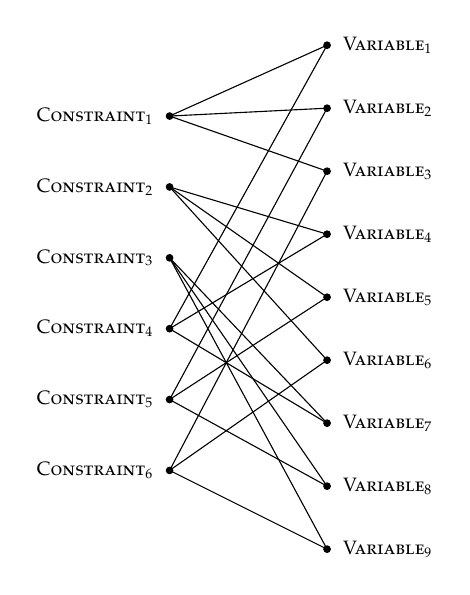
\begin{tikzpicture}[scale=.8]

    \tikzset{type/.style args={[#1]#2}{
        draw,circle,fill,scale=0.25,
        label={[font=\scriptsize, label distance=1pt]#1:#2}
      }}

    % Graph for MS

    \foreach \i in {1,...,6} \draw (0,8-9/8*\i)
    coordinate (Constraint-\i)
    node[type={[180]$\Constraint_\i$}] {};

    \foreach \i in {1,...,9} \draw (2.5,9-\i)
    coordinate (Variable-\i)
    node[type={[0]$\Variable_\i$}] {};

    \foreach \i in {1,...,3} \foreach \j in {1,...,3}
    \pgfmathsetmacro{\k}{(\i-1)*3+\j}
    \draw (Constraint-\i) -- (Variable-\k);

    \foreach \i in {4,...,6} \foreach \j in {1,...,3}
    \pgfmathsetmacro{\k}{\i-3+(\j-1)*3}
    \draw (Constraint-\i) -- (Variable-\k);
  \end{tikzpicture}
  \caption{Type graph $G^\ms$ for the Magic Square game.  }
  \label{fig:type-graph-ms}
\end{figure}

The following theorem records the self-testing (also known as \emph{rigidity})
properties of the Magic Square game.
Although we do not explicitly refer to the theorem, its self-testing properties
are crucial to the Pauli basis test.
In particular, it is used to enforce anticommutation relations between certain
pairs of operators.

\begin{theorem}[Rigidity of the Magic Square game]
  \label{thm:ms-rigidity}
	Let $\strategy = (\ket{\psi}, M)$ be the partial strategy where $\ket{\psi} =
  \ket{\EPR_2}^{\otimes 2}$ and for all $b \in \{0, 1\}$,
  \begin{equation*}
		M^{\Variable_1}_{\, b} = \sigma^{X}_b \otimes I \qquad \text{and}
    \qquad M^{\Variable_5}_{\, b} = \sigma^{Z}_b \otimes I\;,
  \end{equation*}
	where $\sigma^X_b, \sigma^Z_b$ are the $X$ and
  $Z$ Pauli projectors over qubits.
  Then $\game_\MS$ is a self-test for
  $\strategy$ with robustness $O(\sqrt{\eps})$.
\end{theorem}
\begin{proof}
  See~\cite{wu2016device}.
\end{proof}

We will need the following theorem,
which shows that any pair of anticommuting observables 
can be used to form a value-$1$ strategy for the Magic Square game.

\begin{theorem}
  \label{thm:ms-from-ac}
  Let $A = \{A_b\}_{b \in \F_2}$ and $B = \{B_b\}_{b \in \F_2}$ be two-outcome
  projective measurements acting on $(\C^q)^{\otimes n}$ which are consistent on
  $\ket{\EPR_q}^{\otimes n}$, and let $\mathcal{O}_A = A_0 - A_1$ and
  $\mathcal{O}_B = B_0 - B_1$ be the corresponding observables.
  Suppose that $\mathcal{O}_A \mathcal{O}_B = -\mathcal{O}_B \mathcal{O}_A$.
  Then there exists a symmetric strategy $\strategy = (\psi, M)$ for the Magic
  Square game with the following properties.
  \begin{enumerate}
  \item $\strategy$ is an SPCC strategy of value $1$.
  \item The state $\ket{\psi}$ has the form $\ket{\psi} = \ket{\EPR_q}^{\otimes
      n} \otimes \ket{\EPR_2}$.
  \item For $b \in \{0,1\}$, we have $M^{\Variable_1}_b = A_b \otimes I$ and
    $M^{\Variable_5}_b = B_b \otimes I$.\label{item:embeds}
  \end{enumerate}
\end{theorem}

\begin{proof}
  The strategy~$\strategy$
  is based on the canonical two-qubit strategy for the Magic Square game as
  described in, for example,~\cite{aravind2002simple}.
  The state is $\ket{\psi} = \ket{\EPR_q}^{\otimes n} \otimes \ket{\EPR_2}$.
  We specify the measurements of~$\strategy$
  in Figure~\ref{fig:ms-operator-soln} as an \emph{operator solution} for the Magic Square game,
  meant to be read as follows:
  each cell contains a two-outcome projective measurement $\{E_0, E_1\}$ on $(\C^q)^{\otimes n} \otimes \C^2$
  written as its \emph{$\pm 1$-valued observable} $E_0 - E_1$.
  When Player~$\alice$ or~$\bob$ receives the question $\Variable_j$ for $j \in \{1, \ldots, 9\}$,
  they measure their share of~$\ket{\psi}$
  using the measurement specified by the cell corresponding to~$\Variable_j$ and receive a single-bit measurement.
  When they receive the question $\Constraint_i$ for $i \in \{1,2,\ldots,6\}$, they
  simultaneously perform the three measurements in the corresponding row or
  column on $\ket{\psi}$ to obtain three bits.
  For example, if Player~$\alice$ receives question~$\Variable_1$,
  they measure~$\ket{\psi}$ using the measurement $\{A_0 \otimes I, A_1 \otimes I\}$
  corresponding to the observable $\cal{O}_A \otimes I$ (where the
  first operator acts on $\ket{\EPR_q}^{\otimes n}$ and the second acts on
  $\ket{\EPR_2}$).
  Similarly, on question~$\Variable_5$,
  they use the measurement $\{B_0 \otimes I, B_1 \otimes I\}$.
  This establishes Item~\ref{item:embeds} of the theorem.
  \begin{figure}[ht!]
    \begin{center}
      \renewcommand{\arraystretch}{2.4}
      \begin{tabularx}{.6\textwidth}{| X | X | X |}
        \hline
        $ \phantom{I\;\;O}\cal{O}_A\, \otimes \; \;I$
        & $ \phantom{\cal{O}_BO} I\;\;\, \otimes \; \sigma^X$
        & $ \phantom{\cal{O}_B\;}\cal{O}_A\, \otimes \; \sigma^X$ \\
        \hline
        $ \phantom{\cal{O}_AO} I\;\;\, \otimes \; \sigma^Z$
        & $ \phantom{I\;\;O}\cal{O}_B\, \otimes \; \;I$
        & $ \phantom{\cal{O}_A\;}\cal{O}_B\, \otimes \; \sigma^Z$ \\
        \hline
        $ \phantom{I\;\;O}\cal{O}_A \, \otimes \; \sigma^Z$
        & $ \phantom{I\;\;O}\cal{O}_B \, \otimes \; \sigma^X$
        & $ \; \cal{O}_A \cal{O}_B \, \otimes \; \sigma^Z \sigma^X$ \\
        \hline
      \end{tabularx}
      \caption{Observables for Magic Square strategy}
      \label{fig:ms-operator-soln}
		\end{center}
  \end{figure}
  
  First, we show that this gives a well-defined strategy.
  The $\Variable_j$ measurements are well-defined because each cell contains a $\pm 1$-valued observable.
  This is obvious for all $j \neq 9$;  when $j = 9$, the bottom-right cell contains $\cal{O}_A \cal{O}_B \otimes \sigma^Z \sigma^X$.
  Because~$\cal{O}_A$ and~$\cal{O}_B$ anti-commute,
  \begin{equation}\label{eq:am-i-hermitian}
  \cal{O}_A \cal{O}_B \otimes \sigma^Z \sigma^X
  = - \cal{O}_A \cal{O}_B \otimes \sigma^X \sigma^Z
  = \cal{O}_B \cal{O}_A \otimes \sigma^X \sigma^Z
  = (\cal{O}_A \cal{O}_B \otimes \sigma^Z \sigma^X)^\dagger.
  \end{equation}
  As a result, this matrix is Hermitian. In addition, 
  \begin{equation*}
  (\cal{O}_A \cal{O}_B \otimes \sigma^Z \sigma^X)^2
  = (\cal{O}_A \cal{O}_B \otimes \sigma^Z \sigma^X) \cdot (\cal{O}_B \cal{O}_A \otimes \sigma^X \sigma^Z)
  = (\cal{O}_A \cal{O}_B \cdot \cal{O}_B \cal{O}_A) \otimes (\sigma^Z \sigma^X \cdot \sigma^X \sigma^Z)
  = I,
  \end{equation*}
  where the first step uses Equation~\eqref{eq:am-i-hermitian}
  and the final step uses the fact that $\cal{O}_A, \cal{O}_B, \sigma^X, \sigma^Z$ are $\pm 1$-valued observables
  and hence square to the identity.
  As a result, this matrix
  is Hermitian and squares to the identity. Therefore, it is a $\pm 1$-valued observable.
  
  As for the $\Constraint_i$ measurements,
  we must show that the three measurements in each row and column are simultaneously measurable.
  This is equivalent to the three $\pm 1$-valued observables being simultaneously diagonalizable,
  which is equivalent to them being pairwise commuting. This can be easily verified for the cases of $i = 1, 2, 4, 5$
  (i.e.\ the first two rows and columns).
  In the case of $i = 3$, commutativity of $\cal{O}_A \otimes \sigma^Z$ and $\cal{O}_B \otimes \sigma^X$ 
  follows from Equation~\eqref{eq:am-i-hermitian}.
  Since these two matrices commute, they also commute with their product 
  $(\cal{O}_A \otimes \sigma^Z)(\cal{O}_B \otimes \sigma^X) = \cal{O}_A \cal{O}_B \otimes \sigma^Z \sigma^X$.
  The case of $i = 6$ is similar.
  
  By construction, $\strategy$ is symmetric, and we have already shown that it is projective.
  It remains to show that it is commuting, consistent, and value~$1$.
  To show that it is commuting,
  it suffices to show that the measurement for each cell
  is simultaneously measurable with all three measurements in its row or column,
  which was already proved above.
  Now we show consistency.
  By linearity, because $A$ and $B$ are consistent on $\ket{\EPR_q}^{\otimes n}$,
  so too are $\cal{O}_A$ and $\cal{O}_B$.
  We claim that this implies the observable in each cell of Figure~\ref{fig:ms-operator-soln} is consistent on $\ket{\psi}$.
  To see why, consider the $j = 9$ case:
  \begin{align*}
  (\cal{O}_A \cal{O}_B \otimes \sigma^Z \sigma^X)_\alice \otimes I_\bob \cdot \ket{\EPR_q}^{\otimes n} \otimes \ket{\EPR_2}
  &= (\cal{O}_A \cal{O}_B \otimes \sigma^Z)_\alice \otimes (I \otimes \sigma^X)_\bob
  		\cdot \ket{\EPR_q}^{\otimes n} \otimes \ket{\EPR_2}\\
  &= (\cal{O}_A \cal{O}_B \otimes I)_\alice \otimes (I \otimes \sigma^X\sigma^Z)_\bob
  		\cdot \ket{\EPR_q}^{\otimes n} \otimes \ket{\EPR_2}\\
  &= (\cal{O}_A \otimes I)_\alice \otimes ( \cal{O}_B \otimes \sigma^X\sigma^Z)_\bob
  		\cdot \ket{\EPR_q}^{\otimes n} \otimes \ket{\EPR_2}\\
  &= I_\alice \otimes (\cal{O}_B \cal{O}_A \otimes \sigma^X\sigma^Z)_\bob
  		\cdot \ket{\EPR_q}^{\otimes n} \otimes \ket{\EPR_2}\\
  &= I_\alice \otimes (\cal{O}_A \cal{O}_B \otimes \sigma^Z \sigma^X)_\bob
  		\cdot \ket{\EPR_q}^{\otimes n} \otimes \ket{\EPR_2}.
  \end{align*}
  The first two steps use the consistency of $\sigma^X, \sigma^Z$ on $\ket{\mathrm{EPR}_2}$,
  the next two use the consistency of $\cal{O}_B, \cal{O}_A$ on $\ket{\mathrm{EPR}_q}^{\otimes n}$,
  and the last step is by Equation~\eqref{eq:am-i-hermitian}.
  The remaining cases of $j \in\{1, \ldots, 8\}$ are similar, and we omit them.
  
  Now, we show that the measurements in $\strategy$ are consistent.
  Let $E = \{E_0, E_1\}$ be any of the measurements in the cells of Figure~\ref{fig:ms-operator-soln}.
  We have shown that $\cal{O}_E = E_0- E_1$ is consistent on $\ket{\psi}$.
  But for each $b \in \{0, 1\}$, $E_b = (E_0 + E_1 + (-1)^b (E_0 - E_1))/2 = (I + (-1)^b \cal{O}_E)/2$, and so each~$E_b$ is consistent on~$\ket{\psi}$ by the following calculation
  \begin{multline*}
  E_b \otimes I_\bob \ket{\psi}
  = \tfrac{1}{2} (I + (-1)^b \cal{O}_E) \otimes I_\bob \ket{\psi}
  = \tfrac{1}{2} \ket{\psi} + \tfrac{1}{2} (-1)^b \cal{O}_E \otimes I_\bob \ket{\psi}\\
  = \tfrac{1}{2} \ket{\psi} + \tfrac{1}{2} (-1)^b I_\alice \otimes \cal{O}_E \ket{\psi}
  = \tfrac{1}{2} I_\alice \otimes (I + (-1)^b \cal{O}_E) \ket{\psi}
  = I_\alice \otimes E_b \ket{\psi},
  \end{multline*}
  where the third equality is by the consistency of~$\cal{O}_E$.
  As a result, the $\Variable_j$ measurements are consistent.
  As for the $\Constraint_i$ measurements,
  each such measurement $\{F_{a, b, c}\}_{a, b, c \in \{0, 1\}}$ is of the form $F_{a, b, c} = E^1_a \cdot E^2_b \cdot E^3_c$,
  where $E_1$, $E_2$, and $E_3$ are $\Variable$ measurements.
  But then consistency of~$F$ follows from the~$\Variable$ consistencies:
  \begin{multline*}
  F_{a, b, c} \otimes I_{\bob} \ket{\psi}
  = (E^1_a \cdot E^2_b \cdot E^3_c)_{\alice} \otimes I_{\bob} \ket{\psi}
  = (E^1_a \cdot E^2_b)_{\alice} \otimes (E^3_c)_{\bob} \ket{\psi}
    = (E^1_a)_{\alice} \otimes (E^3_c \cdot E^2_b)_{\bob} \ket{\psi}\\
        = I_{\alice} \otimes (E^3_c \cdot E^2_b \cdot E^1_a)_{\bob} \ket{\psi}
        = I_{\alice} \otimes (E^1_a \cdot E^2_b \cdot E^2_c)_{\bob} \ket{\psi}
                = I_{\alice} \otimes F_{a, b,c} \ket{\psi},
  \end{multline*}
  where the second-to-last step is because the $\Variable_j$ measurements in the same row or column commute.
  Hence, all measurements are consistent.
  
  Since all measurements are consistent, this
  implies that the answer bit of the player receiving a $\Variable$ question is
  always consistent with the corresponding answer bit of the player receiving
  the $\Constraint$ question.
  Similarly, the answers of the player receiving the $\Constraint$ question
  always satisfy the given constraint; observe that in all rows and the first
  two columns, the observables multiply to $I$, whereas the observables in the
  last column multiply to $-I$.
  This implies that the strategy is value-$1$, concluding the proof.
\end{proof}

\subsection{The Pauli basis test}
\label{sec:pauli-verifier}

We introduce the quantum low-degree test of~\cite{natarajan2018low} in the form
of a slight modification to it by~\cite{NW19} known as the \emph{Pauli basis
  test}.
Informally, the quantum low-degree test asks the players to measure a large
number of qubits and return a highly compressed version of the measurement
outcome.
The Pauli basis test simply asks that the players return their uncompressed
measurement outcomes, and it is designed by direct reduction to the quantum
low-degree test.
In Section~\ref{sec:qld-game} we describe the Pauli basis test as a nonlocal
game $\game^\pauli$, as we did with the classical low-degree test in
Section~\ref{sec:ld-verifier}.
In Section~\ref{sec:qld-cl-funcs}, we describe how to generate questions for the
Pauli basis test using CL functions.
In Section~\ref{sec:qld-complexity} we exhibit canonical parameters for the
Pauli basis test and give bounds on the time complexity of executing the test.

\subsubsection{The game}
\label{sec:qld-game}

We start by discussing parameter settings.
The game $\game^\pauli$ is parametrized by a tuple
\[\qldparams = (q,m,d,h,H,\Gamma,\pi)\;,\] where $q,m,d,h,\Gamma \in \N$ are integers, $H$ is a
subset of $\F_{q}$ of size $h$, and $\pi$ is a map from $\{1, 2, \ldots,
\Gamma\}$ to $H^m$.
We sometimes write $\game^\pauli_\qldparams$ to emphasize the dependence of the
Pauli basis test on the parameters.

Informally, the test is meant to certify that the players share a state of the
form $\ket{\EPR_q}^{\otimes \Gamma}$.
Its question set includes questions that are planes and points in $\F_q^m$,
which are meant to correspond to questions in a low-degree test, and questions
of the form $(\Pauli, W)$, for $W \in \{X, Z\}$.
Upon receipt of a question of the latter form, the players are expected to perform the POVM $\{\tau_u^W\}_{u \in \F_q^{\Gamma}}$ and report the outcome $u$ as
their answer.

\begin{definition}[Admissible parameters]\label{def:admissible}
  We say that the tuple $\qldparams=(q, m, d, h, H, \Gamma, \pi)$ is
  \emph{admissible} if $q$ is an admissible field size, $h \leq q$, and $\Gamma \leq h^m$.
\end{definition}


Similarly to the game $\game^\ld$, questions in the Pauli basis
game come with a ``question type'' part and a ``question content'' part. The question types are taken from the set
\begin{equation}
  \label{eq:pauli-type}
  \type^\pauli= \bigl( \{\Point, \Plane, \Pauli, \Pair \} \times \{X,Z\} \bigr)
  \cup \type^\ms \cup \{\Pair\}\;,
\end{equation}
where $\type^\ms$ is the question type set of the Magic Square game defined in
Section~\ref{sec:ms}.
The question content has a format that depends on the type.

\begin{figure}[!htbp]
  \centering
  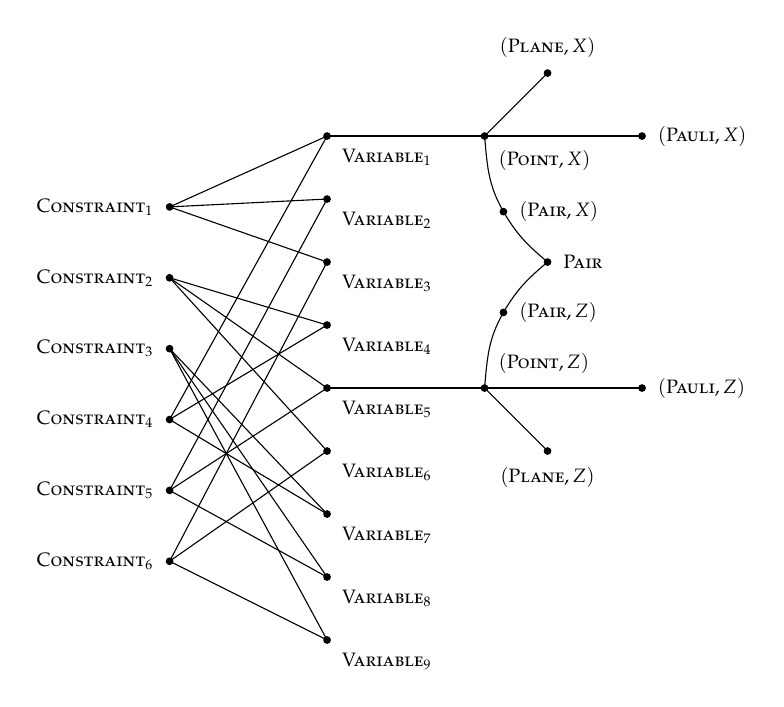
\begin{tikzpicture}[scale=.8]

    \tikzset{type/.style args={[#1]#2}{
        draw,circle,fill,scale=0.25,
        label={[font=\scriptsize, label distance=1pt]#1:#2}
      }}

    % Graph for MS

    \foreach \i in {1,...,6} \draw (0,8-9/8*\i)
    coordinate (Constraint-\i)
    node[type={[180]$\Constraint_\i$}] {};

    \foreach \i in {1,...,9} \draw (2.5,9-\i)
    coordinate (Variable-\i)
    node[type={[330]$\Variable_\i$}] {};

    \foreach \i in {1,...,3} \foreach \j in {1,...,3}
    \pgfmathsetmacro{\k}{(\i-1)*3+\j}
    \draw (Constraint-\i) -- (Variable-\k);

    \foreach \i in {4,...,6} \foreach \j in {1,...,3}
    \pgfmathsetmacro{\k}{\i-3+(\j-1)*3}
    \draw (Constraint-\i) -- (Variable-\k);

    % Types for QLD

    \draw (6,9) coordinate (Plane-X) node[type={[90]$(\Plane, X)$}] {};
    \draw (5,8) coordinate (Point-X) node[type={[315]$(\Point, X)$}] {};
    \draw (7.5,8) coordinate (Pauli-X) node[type={[0]$(\Pauli, X)$}] {};
    \draw (6,3) coordinate (Plane-Z) node[type={[270]$(\Plane, Z)$}] {};
    \draw (5,4) coordinate (Point-Z) node[type={[45]$(\Point, Z)$}] {};
    \draw (7.5,4) coordinate (Pauli-Z) node[type={[0]$(\Pauli, Z)$}] {};
    \draw (6,6) coordinate (Pair) node[type={[0]$\Pair$}] {};
    \draw (5.3,6.8) coordinate (Pair-X) node[type={[0]$(\Pair,X)$}] {};
    \draw (5.3,5.2) coordinate (Pair-Z) node[type={[0]$(\Pair,Z)$}] {};

    % Edges

    \foreach \from/\to in {Plane-X/Point-X, Point-X/Pauli-X,
      Plane-Z/Point-Z, Point-Z/Pauli-Z,
      Point-X/Variable-1, Point-Z/Variable-5}
    \draw (\from) -- (\to);

    \draw (Point-X) to [out=275,in=120] (Pair-X) to [out=300,in=140] (Pair);
    \draw (Point-Z) to [out=85,in=240] (Pair-Z) to [out=60,in=220] (Pair);

  \end{tikzpicture}
  \caption{Graph $G^\pauli$ for the Pauli basis test.
    Each vertex also has a self-loop which is not drawn on the figure for
    clarity.}
  \label{fig:type-graph-pauli}
\end{figure}

The distribution $\mu_\pauli$ over questions $((\tvar_\alice, x_\alice),
(\tvar_\bob, x_\bob))$ in $\game^\pauli$ is defined through the following
sampling procedure:
\begin{enumerate}
\item Sample a pair of types by sampling an edge $(\tvar_\alice, \tvar_\bob)$ of
  the graph $G^\pauli$ given in Figure~\ref{fig:type-graph-pauli} uniformly at
  random (including the self-loops).
\item Sample the following uniformly at random:
	\begin{enumerate}
	\item (\emph{Points}) $u_\xpt,u_\zpt \in \F_q^m$,
  \item (\emph{Directions}) $v_1, v_2 \in \F_q^m$,
  \item (\emph{Qubit basis for (anti-)commutation}) $r_\xpt,r_\zpt \in \F_q$.
	\end{enumerate}
\item For $w \in \AB$ and $W\in\{X,Z\}$,
	\begin{enumerate}
  \item If $\tvar_w = (\Point, W)$, then set $x_w = u_W$,
  \item If $\tvar_w = (\Plane, W)$, then set $x_w = (u,v_1,v_2)$, where $u =
    L^\plf_{v_1,\, v_2}(u_W)$,
  \item If $\tvar_w = \Constraint_i$ for some $i\in\{1,\ldots,6\}$, then set
    $x_w = (u_\xpt, u_\zpt, r_\xpt, r_\zpt)$,
  \item If $\tvar_w = \Variable_j$ for some $j\in\{1,\ldots,9\}$, then set $x_w
    = (u_\xpt, u_\zpt, r_\xpt, r_\zpt)$,
  \item If $\tvar_w = \Pair$, then set $x_w = (u_\xpt, u_\zpt, r_\xpt, r_\zpt)$,
  \item If $\tvar_w = (\Pair, W)$, then set $x_w = (u_\xpt, u_\zpt, r_\xpt, r_\zpt)$,
  \item If $\tvar_w = (\Pauli, W)$, then set $x_w = 0$.
	\end{enumerate}
\end{enumerate}
As with the game $\game^\ld$, the question content is a bit string that is
interpreted as a vector over $\F_q$ (as described in
Section~\ref{sec:ff-representations}).

\paragraph{Decision procedure.}
The decision procedure for $\game^\pauli$ is presented in
Figure~\ref{fig:decider_pauli}.
Similarly to Figure~\ref{fig:ld-decider}, we provide a table that summarizes a
parsing scheme for the questions and answers, depending on the type of question.
The answers are bit strings that are interpreted as more structured objects such
as elements over $\F_q$, vectors, or polynomials, depending on the question.
In the ``low-degree check'', the decision procedure $\decider^\pauli$ calls the
classical low-degree decision procedure $\decider^\ld$ parametrized by the tuple
$\ldparams = (q,m,d,1)$ (defined in Section~\ref{sec:ld-verifier}) as a
subroutine.

\begin{figure}[htbp!]
  \begin{gamespec}
    \vspace{9pt}
    \begin{center}
      \renewcommand\arraystretch{1.3}
      \begin{tabularx}{.92\textwidth}{ l X l }
        \toprule
        Type & Question Content & Answer Format \\
        \midrule
        (\Point, $W$) & $y \in  \F_q^m$ & Element of $\F_q$  \\
        (\Plane, $W$) & $v = (u_W, v_1, v_2) \in (\F_q^m)^3$
        & Polynomial $f: \pl(v) \to \F_q$\\
        \Pair & $(u_\xpt, u_\zpt, r_\xpt, r_\zpt) \in
        (\F_q^m)^2 \times \F_q^2 $ & $(\beta_\xpt,\beta_\zpt) \in \F_2^2$ \\
        (\Pair, $W$) & $(u_\xpt, u_\zpt, r_\xpt, r_\zpt) \in
        (\F_q^m)^2 \times \F_q^2 $ & Element of $\F_2$ \\
        $\Constraint_i$ & $(u_\xpt, u_\zpt, r_\xpt, r_\zpt) \in (\F_q^m)^2
        \times \F_q^2$ &
        $(\alpha_{v_1}, \alpha_{v_2}, \alpha_{v_3}) \in \F_2^3$ \\
        $\Variable_j$ & $(u_\xpt, u_\zpt, r_\xpt, r_\zpt) \in
        (\F_q^m)^2 \times \F_q^2$ & Element of $\F_2$ \\
        (\Pauli, $W$) & $0$ & Element of $\F_q^{\Gamma}$ \\
        \bottomrule \multicolumn{3}{c}{Table: Question and answer format of the
          Pauli basis game.}
      \end{tabularx}
    \end{center}
    \vspace{9pt}

    On input $(\tvar_\alice,x_\alice, \tvar_\bob, x_\bob, a_\alice, a_\bob)$,
    the decision procedure $\decider^\pauli$ performs the following checks for
    $w \in \AB$:
    \begin{enumerate}[itemsep=2pt,parsep=2pt]
    \item (\textbf{Consistency check}).
      \label{item:same-type}
      If $\tvar_\alice = \tvar_\bob$, accept iff $a_\alice = a_\bob$.

    \item (\textbf{Low-degree check}).
      \label{item:low-degree}
      If $\tvar_w = (\Point, W), \tvar_{\overline{w}} = (\Plane, W)$, accept if
      $\decider^\ld_{\ldparams}$ accepts $(\tvar_w, x_w, \tvar_{\overline{w}}, x_{\overline{w}}, a_w,
      a_{\overline{w}})$ 
%      \hnote{I think the arguments should be $(x_w,x_{\overline{w}},a_w,a_{\overline{w}})$, because passing $\pl(v)$ as an argument doesn't make sense.... $\pl(v)$ is a set of points (see the beginning of this section).}, 
with $\ldparams = (q,m,d,1)$.

    \item (\textbf{Consistency check}).
      \label{item:low-degree-consistency}
      If $\tvar_w = (\Point, W), \tvar_{\overline{w}} = (\Pauli, W)$, accept if
      $g_{a_{\overline{w}},\, \pi}(y) = a_w$, where $g_{a_{\overline{w}},\, \pi}$ is
      the low-degree encoding of $a_{\overline{w}} \in \F_q^\Gamma$ defined in
      Section~\ref{sec:ld-encoding}.
    \end{enumerate}
    In the remaining three cases, the decision procedure first computes the number
    \begin{equation}
      \label{eq:gamma-value}
      \gamma = \tr \bigl( (\ind_{H, m,\pi}(u_\xpt) r_\xpt) \cdot
      (\ind_{H,m, \pi}(u_\zpt) r_\zpt) \bigr)\;,
    \end{equation}
    where we recall the $\ind_{H, m, \pi}(\cdot)$ notation from Section~\ref{sec:ld-encoding}.
    \begin{enumerate}[itemsep=2pt,parsep=2pt]
      \setcounter{enumi}{3}
    \item (\textbf{Commutation check}).
      \label{item:commutation} If $\tvar_w = (\Pair, W), \tvar_{\overline{w}} =
      \Pair$, accept if $a_w = \beta_W$ or $\gamma \neq 0$.
    \item (\textbf{Consistency check}).
      \label{item:commutation-consistency} If $\tvar_w = (\Point,W), \tvar_{\overline{w}} =
      (\Pair,W)$, accept if $\tr (a_w r_W) = a_{\overline{w}}$ or $\gamma \neq 0$.
      
    \item (\textbf{Magic square check}).
      \label{item:magic-square} If $\tvar_w = \Constraint_i,
      \tvar_{\overline{w}} = \Variable_j$, accept if $\gamma = 0$, or $a_w$
      satisfies constraint $\Constraint_i$ and $ \alpha_j = a_{\overline{w}}$.

    \item (\textbf{Consistency check}).
      \label{item:magic-square-consistency}
      If $\tvar_w = (\Point,W), \tvar_{\overline{w}} = \Variable_j$, accept if
      $\gamma = 0$ or if $j = 1$, $W = X$, and $\tr(a_w r_\xpt) =
      a_{\overline{w}}$ or if $j = 5$, $W = Z$, and $\tr(a_w r_\zpt) =
      a_{\overline{w}}$.
    \end{enumerate}
  \end{gamespec}
  \caption{Specification of the decision procedure $\decider^\pauli_\qldparams$.}
  \label{fig:decider_pauli}
\end{figure}

We describe an honest, value-$1$ PCC strategy for the Pauli basis test.

\begin{definition}
  \label{def:honest-pauli-strategy}
  Let $\qldparams = (q,m,d,h,H,\Gamma,\pi)$ be a parameter tuple.
  Define the \emph{honest Pauli strategy corresponding to $\qldparams$} as a
  partial strategy $\strategy^\pauli$ that uses the state $\ket{\EPR_q}^{\otimes
    \Gamma}$ and uses the POVM $\{\tau^W_u\}_{u\in \F_q^{\Gamma}}$ for the
  question $(\Pauli, W)$ for $W\in \{X,Z\}$.
\end{definition}

\begin{lemma}\label{lem:pauli-completeness}
  The Pauli basis test $\game^\pauli_\qldparams$ has a value-$1$ SPCC strategy.
\end{lemma}

\begin{proof}
  We begin by specifying the value-$1$ strategy $\strategy = (\ket{\psi}, M)$.
  The state is
  \begin{equation*}
    \ket{\psi} = \ket{\EPR_q}^{\otimes \Gamma} \otimes \ket{\EPR_2}\;.
  \end{equation*}
  Now we specify the measurements.
  We start with measurements associated with questions of type $\Point$,
  $\Plane$, and $\Pauli$.
  Using notation introduced in Section~\ref{sec:ld-encoding}, for $W \in \{X,
  Z\}$,
  \begin{align*}
    M^{(\Point,W),\, y}_{\, a}
    & = \tau^W_{[g_{\cdot,\, \pi}(y) = a]} \otimes I\;,\\
    M^{(\Plane,W),\, \pl}_{\, f}
    & = \tau^W_{[(g_{\cdot,\, \pi})|_\pl = f]} \otimes I\;,\\
    M^{(\Pauli,W)}_{\, a}
    & = \tau^W_{a} \otimes I\;.
  \end{align*}
  We recall  Definition~\ref{def:plane-point} for the notation $\pl$ and Definition~\ref{def:bracket} for the bracket notation used to post-process measurement outcomes.
  For example, the measurement on question $(\Point,W)$
  corresponds to first performing the measurement $\{\tau^W_w\}_{w \in \F_q^\Gamma}$,
  receiving an outcome $w \in \F_q^\Gamma$,
  and then outputting the value $a = g_{w, \pi}(y)$.  
  Next we specify the POVMs associated with questions of type $\Constraint$,
  $\Variable$, and $\Pair$.
  Questions with these question types have a question content that is a tuple
  $\omega= (u_\xpt, u_\zpt, r_\xpt, r_\zpt)\in (\F_q^m)^2 \times \F_q^2$.
  Given such a tuple, consider the two $\F_2$-valued POVMs $A=\{A_b\}_{b \in
    \F_2}$ and $B=\{B_b\}_{b \in \F_2}$ defined as
  \begin{align}
    A_b & = \tau^X_{[\tr(g_{\cdot,\, \pi}(u_X)\, r_\xpt) = b]} \otimes I\;,\label{eq:gonna-expand-A}\\
    B_b & = \tau^Z_{[\tr(g_{\cdot,\, \pi}(u_Z)\, r_\zpt) = b]} \otimes I\;.\label{eq:gonna-expand-B}
  \end{align}
We would like to determine when 
  the two observables $\mathcal{O}_A = A_0 -
    A_1$ and $\mathcal{O}_B = B_0 - B_1$ commute or anti-commute.
  Towards this we derive alternative expressions for these observables from which their commutativity becomes plain from inspection.
  We begin by inspecting the first matrices on the right-hand sides of Equations~\eqref{eq:gonna-expand-A}
  and~\eqref{eq:gonna-expand-B}:
  \begin{align}
  \tau^W_{[\tr(g_{\cdot,\, \pi}(u_W)\, r_W) = b]}
  &= \sum_{w : \tr(g_{w,\, \pi}(u_W)\, r_W) = b} \tau^W_w\nonumber\\
  &= \sum_{w : \tr((w\, \cdot\, \ind_{H, m, \pi}(u_W)) \cdot r_W ) = b} \tau^W_w\;,\label{eq:expand-with-dot-product}
  \end{align}
  where~\eqref{eq:expand-with-dot-product}
  follows by  Definition~\ref{eq:low-degree-encoding-definition}.
  As a result,
  \begin{align}
  \tau^W_{[\tr(g_{\cdot,\, \pi}(u_W)\, r_W) = 0]}
  -   \tau^W_{[\tr(g_{\cdot,\, \pi}(u_W)\, r_W) = 1]}
  & = \sum_{w : \tr((w\, \cdot\, \ind_{H, m, \pi}(u_W)) \cdot r_W ) = 0} \tau^W_w
  	- \sum_{w : \tr((w\, \cdot\, \ind_{H, m, \pi}(u_W)) \cdot r_W ) = 1} \tau^W_w\nonumber\\
  & = \sum_{w} (-1)^{\tr((w\, \cdot\, \ind_{H, m, \pi}(u_W)) \cdot r_W )} \tau^W_w\nonumber\\
  & = \tau^W(\ind_{H, m, \pi}(u_W)r_W)\;,\label{eq:finally-got-an-observable}
  \end{align}
  where the last step uses~\eqref{eq:pauli-obs-proj}.
  As a result, Equation~\eqref{eq:finally-got-an-observable}
  and Equations~\eqref{eq:gonna-expand-A} and~\eqref{eq:gonna-expand-B} imply that
  \begin{equation*}
  \mathcal{O}_A = \tau^X(\ind_{H, m, \pi}(u_X)r_X) \otimes I,\quad
  \mathcal{O}_B = \tau^Z(\ind_{H, m, \pi}(u_Z)r_Z) \otimes I\;.
  \end{equation*}
  Now, let $\gamma = \tr((\ind_{H, m, \pi}(u_X)r_X) \cdot (\ind_{H, m, \pi}(u_Z)r_Z)) \in \F_2$,
  as in Equation~\eqref{eq:gamma-value}.
  Then by Equation~\eqref{eq:twisted-fq},
  \begin{equation*}
  \mathcal{O}_A \mathcal{O}_B = (-1)^{\gamma} \mathcal{O}_B \mathcal{O}_A\;.
  \end{equation*}
  As a result, $\gamma$ quantifies whether the observables $\mathcal{O}_A$ and $\mathcal{O}_B$ commute,
  and therefore whether the measurements~$A$ and~$B$ commute.
  If $\gamma = 0$, they commute. If $\gamma = 1$, they anti-commute.
  We now specify the  POVMs associated with questions of type $\Constraint$,
  $\Variable$, and $\Pair$, 
  considering separately the cases when $\gamma = 0$ or $\gamma = 1$.
  \begin{enumerate}
  \item If $\gamma = 0$, 
     for each $\beta_X, \beta_Z \in \F_2$ define
    \begin{equation}\label{eq:pair-definition}
      M^{\Pair,\, \omega}_{\beta_X,\, \beta_Z} = A_{\beta_X} \cdot B_{\beta_Z}\;,
    \end{equation}
    \begin{equation*}
      M^{(\Pair,X),\, \omega}_{a} = A_{a} \;,\qquad
      M^{(\Pair,Z),\, \omega}_{a} = B_{a}\;.
    \end{equation*}
    The POVM associated with questions of type $\Constraint$ and $\Variable$ are
    defined to be trivial.
    In particular, we define
    \begin{equation*}
      M^{\Constraint_i,\, \omega}_{\, 0,\, 0,\, 0}
      = M^{\Variable_j,\, \omega}_{\, 0} = I\;,
    \end{equation*}
    and the remaining POVM elements in these measurements are set to be zero.
  \item If $\gamma = 1$, then $\mathcal{O}_A$ and $\mathcal{O}_B$ anti-commute.
    In this case we define measurements $M^{\Constraint_i,\, \omega}$ and
    $M^{\Variable_j,\, \omega}$, for all $i\in\{1,\ldots,6\}$ and $j
    \in\{1,\ldots,9\}$ to be those guaranteed by Theorem~\ref{thm:ms-from-ac}.
    Measurements associated with inputs of type $\Pair$ are defined to be
    trivial.
    In particular, we define
    \begin{equation*}
      M^{\Pair,\, \omega}_{0,\, 0} = M^{(\Pair,X),\, \omega}_{0} = M^{(\Pair,Z),\, \omega}_{0} = I\;,
    \end{equation*}
    and the remaining matrices in these measurements are set to be zero.
  \end{enumerate}
  This completes the specification of the strategy.

  Now, we show that $\strategy$ is a value-$1$ SPCC strategy.
  It is clearly symmetric and projective. 
  To show that it is consistent, we note that all measurements are Pauli basis measurements, which are consistent,
  or measurements produced by Theorem~\ref{thm:ms-from-ac}, which are also consistent.
  The only exception is the $\Pair$ measurement in the $\gamma = 0$ case, which by Equation~\eqref{eq:pair-definition}
  is a product of two commuting, consistent measurements, and so it is therefore also consistent.
  To show that it is commuting,
  we note that for each $W \in \{X, Z\}$, all $(\Point, W)$, $(\Plane, W)$, and $(\Pauli, W)$ measurements commute
  as they are all measurements in the Pauli~$W$ basis.
  Next, if $\gamma = 0$ then the $\Constraint$ and $\Variable$ measurements commute trivially,
  and for $W \in \{X, Z\}$, the $(\Point, W)$ measurement commutes with the $(\Pair, W)$ measurement,
  as they are both $W$ basis measurements,
  and the measurement $M^{\Pair, \omega}_{\beta_X, \, \beta_Z} = A_{\beta_X}\cdot B_{\beta_Z}$ 
  commutes with $M^{(\Pair, W), \omega}_{a}$ because $A$ and~$B$ commute.
  On the other hand, if $\gamma = 0$, then the $\Pair$ measurements commute trivially,
  and the $\Constraint$ and $\Variable$ measurements commute by Theorem~\ref{thm:ms-from-ac}.
  Finally, the $(\Point, X)$ measurement commutes with $\Variable_1$ because both are $X$-basis measurements,
  and likewise both $(\Point, Z)$ and $\Variable_5$ are $Z$-basis measurements.
  
  It remains to show that $\strategy$ is value-$1$.
	Consider first the first three tests executed by the decision procedure in
  Figure~\ref{fig:decider_pauli}.
  The strategy passes the consistency checks with probability~$1$ because it is
  projective and consistent.
  It passes the low-degree checks because it answers those consistently with an
  honest strategy in the classical low-degree test.
		
  Next, consider the remaining four tests.
  Fix an $\omega= (u_\xpt, u_\zpt, r_\xpt, r_\zpt)$ and~$\gamma$ as
  in~\eqref{eq:gamma-value}.
  If $\gamma = 0$, then the strategy passes the commutation check with
  probability~$1$ by construction.
  As for the consistency check in Item~\ref{item:commutation-consistency},
  we can write the $(\Point, W)$ measurement as follows: 
  \begin{equation*}
  M^{(\Point,W),\, y}_{[\tr(\,\cdot\, r_W) = a_{\overline{w}}]}
  = \tau^W_{[\tr(g_{\cdot,\, \pi}(y)r_W) = a_{\overline{w}}]} \otimes I
  = M^{(\Pair, W), \omega}_{a_{\overline{w}}} \otimes I.
  \end{equation*}
  As a result, due to the consistency of the $(\Pair, W)$ measurement, the consistency check is passed with probability~$1$.
  On the other hand, if $\gamma \neq 0$,
  then the strategy passes the Magic Square check by Theorem~\ref{thm:ms-from-ac}.
  As for the consistency check in Item~\ref{item:magic-square-consistency},
  we can write the $(\Point, X)$ measurement as follows: 
  \begin{equation*}
  M^{(\Point,X),\, y}_{[\tr(\,\cdot\, r_X) = a_{\overline{w}}]}
  = \tau^X_{[\tr(g_{\cdot,\, \pi}(y)r_X) = a_{\overline{w}}]} \otimes I
  = M^{\Variable_1,\, \omega}_{a_{\overline{w}}} \otimes I,
  \end{equation*}
  where the last step is by Theorem~\ref{thm:ms-from-ac}.
  As these measurements are consistent, this test is passed with probability~$1$.
\end{proof}

As described in Definition~\ref{def:honest-pauli-strategy}, the strategy
$\strategy^\pauli$ is a strategy that uses qudit Pauli measurements and
maximally entangled states defined over qudits with dimension larger than $2$.
However, it is more convenient for our application of the Pauli basis test to
have a self-test for \emph{qubits}.
In particular, we use the Pauli basis test in the ``introspection game'' of
Section~\ref{sec:introspection}, where the players are commanded to sample
questions according to a sampler $\sampler$ of a normal form verifier.
By definition of normal form verifier, $\sampler$ is a sampler over $\F_2$, and
therefore it is natural to use a test for qubit Pauli observables.
This motivates the definition of a \emph{binary Pauli strategy}:

\begin{definition}
  \label{def:binary-pauli-strategy}
  Let $\qldparams = (q,m,d,h,H,\Gamma,\pi)$ be a parameter tuple.
  Define the \emph{honest binary Pauli strategy corresponding to $\qldparams$}
  as the partial strategy $\strategy^\bp$ that uses the state
  $\ket{\EPR_2}^{\otimes \Gamma \log q}$ and uses the POVM $\{\sigma^W_u\}_{u\in
    \F_2^{\Gamma \log q}}$ for the question $(\Pauli, W)$ for $W\in \{X,Z\}$.
  Here, $\sigma^W_u$ denotes the tensor product of qubit Pauli projectors
  $\bigotimes_i \sigma^W_{u_i}$.
\end{definition}

Since we use field sizes that are powers of $2$, Lemma~\ref{lem:pauli-binary}
shows that the strategy $\strategy^\pauli$ based on qudits is isomorphic
to the strategy $\strategy^\bp$ based on qubits.

% The next lemma shows that, since we restrict to using field sizes that are
% powers of $2$, the strategy $\strategy^\pauli$ is isomorphic to a strategy
% using qubits Pauli measurements and maximally entangled states over qubits.

\paragraph{Soundness of the Pauli basis test.} 
We now state the soundness properties of the Pauli basis test.
The following is an adaptation of the self-testing statement in~\cite[Theorem
6.4]{NW19}.

\begin{theorem}
  \label{thm:pauli}
	There exists a function $\delta(\eps,m,d,q) = a (\eps + md/q^c)^{b}$ for
  universal constants $a,b,c > 0$ such that the following holds.
  Let $\qldparams = (q,m,d,h,H,\Gamma,\pi)$ be an admissible parameter tuple and
  let $\strategy^\pauli$ be the honest Pauli strategy corresponding to
  $\qldparams$.
  The game $\game^\pauli_\qldparams$ is a self-test for the honest binary Pauli
  strategy $\strategy^\bp$ corresponding to $\qldparams$ with robustness
  $\delta(\eps,m,d,q)$.
\end{theorem}

\begin{proof}
	This follows from~\cite[Theorem 6.4]{NW19}, which states that the game
  $\game^\pauli_\qldparams$ is a self-test for the honest Pauli strategy
  $\strategy^\pauli$ corresponding to $\qldparams$ with robustness
  $\delta(\eps,m,d,q)$, and Lemma~\ref{lem:pauli-binary}, which states that
  $\strategy^\pauli$ is isomorphic to the honest {binary} Pauli strategy
  $\strategy^\bp$ corresponding to $\qldparams$.
\end{proof}

\subsubsection{Conditional linear functions for the Pauli basis test}
\label{sec:qld-cl-funcs}

We define CL functions that allow us to specify the distribution $\mu_\pauli$ of
the Pauli basis test as a (typed) CL distribution.
These CL functions will be used in the sampler for the introspective verifier in
Section~\ref{sec:introspection}.

Fix a parameter tuple $\qldparams = (q,m,d,h,H,\Gamma,\pi)$.
Let $V^\pauli$ denote the linear space $\F_q^s$ for $s = 4m + 2$.
The space $V^\pauli$ is decomposed into a direct sum of the following register
subspaces: $V_\xpt,V_\zpt,V_{\dir{1}},V_{\dir{2}}$ (which are $m$-dimensional),
and $V_{\rxpt},V_{\rzpt}$ (which are $1$-dimensional).
We define CL functions $L^\tvar: V^\pauli \to V^\pauli$ for every type $\tvar
\in \type^\pauli$:
\begin{enumerate}
\item If $\tvar = (\Point,W)$ for some $W \in \{X,Z\}$, then $L^{\Point,W}$ is
  the $1$-level CL function $L^\ptf$ (from Section~\ref{sec:ld-cl-funcs})
  parameterized by field size $q$, dimension $m$, and point register
  $V_W$.% and direction registers $V_{\dir{1}},V_{\dir{2}}$.

\item If $\tvar = (\Plane,W)$ for some $W \in \{X,Z\}$, then $L^{\Point,W}$ is
  the $2$-level CL function $L^\plf$ (from Section~\ref{sec:ld-cl-funcs})
  parameterized by field size $q$, dimension $m$, point register $V_W$, and
  direction registers $V_{\dir{1}},V_{\dir{2}}$.

\item If $\tvar = \Constraint_i$ for $i \in \{1, 2, \ldots, 6\}$, then the
  $1$-level CL function $L^{\Constraint_i}$ is the projector onto $V_\xpt \oplus
  V_\zpt \oplus V_{\rxpt} \oplus V_{\rzpt}$.
	
\item If $\tvar = \Variable_j$ for $j \in \{1,2,\ldots,9\}$, then the $1$-level
  CL function $L^{\Variable_j}$ is the projection onto $V_\xpt \oplus V_\zpt
  \oplus V_{\rxpt} \oplus V_{\rzpt}$.
	
\item If $\tvar = \Pair$, then the $1$-level CL function $L^{\Pair}$ is the
  projection onto $V_\xpt \oplus V_\zpt \oplus V_{\rxpt} \oplus V_{\rzpt}$.
  
 \item If $\tvar = (\Pair,W)$, then the $1$-level CL function $L^{\Pair,W}$ is the
  projection onto $V_\xpt \oplus V_\zpt \oplus V_{\rxpt} \oplus V_{\rzpt}$.

\item If $\tvar = (\Pauli,W)$ for some $W \in \{X,Z\}$, then the $0$-level CL
  function $L^{\Pauli,W}$ is identically $0$.
\end{enumerate}

Let $\nu$ denote the typed CL distribution on $\type^\pauli \times V^\pauli
\times \type^\pauli \times V^\pauli$ where
$(\tvar_\alice,x_\alice,\tvar_\bob,x_\bob)$ is sampled by first uniformly
sampling an edge $(\tvar_\alice,\tvar_\bob)$ from the graph $G^\pauli$ defined
in Figure~\ref{fig:type-graph-pauli}, sampling a uniformly random $z \in
V^\pauli$, and then setting $x_w = L^{\tvar_w}(z)$ for $w \in \AB$.

\begin{lemma}\label{lem:pauli-basis-sampler}
 The distribution $\nu$ is a
  $2$-level typed CL distribution.
  Furthermore, let $(\tvar_\alice,x_\alice,\tvar_\bob,x_\bob)$ be sampled from
  $\mu_\pauli$ described in Section~\ref{sec:qld-game}.
  For $w\in\{\alice,\bob\}$ let $\tilde{x}_w$ be the vector $x_w$, seen as an
  element of $V^\pauli$ (i.e.\ the vector is padded with zeroes whenever
  necessary).
  Then the distribution of
  $(\tvar_\alice,\tilde{x}_\alice,\tvar_\bob,\tilde{x}_\bob)$ is identical to
  the distribution $\nu$.
\end{lemma}

\begin{proof}
  That $\nu$ is $2$-level is immediate from the description.
  To see that the distributions are identical, the random vectors
  $u_\xpt,u_\zpt,v_1,v_2,r_\xpt,r_\zpt$ sampled in the description of
  $\mu_\pauli$ correspond, in the description of $\nu$, to the projection of the
  random vector $z \in V^\pauli$ to the register subspaces $V_\xpt$, $V_\zpt$,
  $V_{\dir{1}}$, $V_{\dir{2}}$, $V_{\rxpt}$, and $V_{\rzpt}$ respectively.
\end{proof}
	
\subsubsection{Canonical parameters and complexity of the Pauli basis test}
\label{sec:qld-complexity}

We specify a canonical setting of the parameter tuple $\qldparams$ as a function
of an integer $r$.
We then give bounds on the complexity of computing the decision procedure and CL
functions of the Pauli basis test corresponding to the parameter tuple
$\qldparams$, as a function of $r$.

\begin{definition}[Canonical parameters of the Pauli basis test]
  \label{def:introparams}
  Let $c_0$ denote the smallest of the universal constants $a,b,c$ specified in
  Theorem~\ref{thm:pauli}, and let $c_1 = \max\{c_0,2\}$.
  For all integers $r \in \N$, define the tuple $\introparams(r) =
  (q,m,d,h,H,\Gamma,\pi)$ where 
  \begin{gather*}
    k =  2 \lceil c_1  \log r  \rceil + 1, \qquad q=2^{k}, \qquad
    \Gamma = \lceil r/\log q \rceil + 1, \qquad
    m = \left \lceil \frac{2}{c_0} \cdot
      \frac{\log \Gamma}{\log r} \right \rceil,
  \end{gather*}
  and, using notation from Section~\ref{sec:canonical-injection}, define $H =
  \canH{m}{k}{\Gamma} \subseteq \F_q$, $h = \canlilh{m}{k}{\Gamma} = |H|$, $\pi:\{1, 2,\ldots, \Gamma\} \rightarrow H^m$
  as
  \begin{equation*}
  \pi(i) = \canin{m}{k}{\Gamma}(i-1)
  \end{equation*}
  for $i \in \{1, 2, \ldots, \Gamma\}$,
  where $\canin{m}{k}{\Gamma}:\{0, 1, \ldots, \Gamma-1\} \rightarrow H^m$, and $d =
  m(h-1)$.
\end{definition}

Intuitively, this choice of parameter settings is such that the Pauli basis test
certifies the presence of an $r$-qubit EPR state.

\begin{lemma}
  \label{lem:delta-bound}
  For all integers $r \in \N$, the parameter tuple $\introparams(r)$ is
  admissible (see Definition~\ref{def:admissible}), and furthermore there exist
  universal constants $a',b' > 0$ such that the function $\delta(\eps, m, d, q)$
  from Theorem~\ref{thm:pauli} is at most $a' (\eps + \frac{1}{r})^{b'}$.
\end{lemma}

\begin{proof}
  We verify the admissibility of $\introparams(r)$ first.
  The field size $q = 2^k$ is admissible because $k$ is odd.
  Fix $r \in \N$.
  From the definition of $\canlilh{m}{k}{\Gamma}$ in
  Section~\ref{sec:canonical-injection}, we get that
  \[
    h = \canlilh{m}{k}{\Gamma} = 2^{\lceil b(\Gamma)/m \rceil}
  \]
  where $b(\Gamma) = \lfloor \log (\Gamma - 1) + 1 \rfloor$.
  Therefore $h^m \geq 2^{b(\Gamma)} \geq \Gamma$ and
  \begin{equation}
    \label{eq:h-bound}
    \log h \leq \frac{b(\Gamma)}{m} \leq \frac{c_0}{2} \cdot
    \frac{1 + \log (\Gamma-1)}{\log \Gamma} \cdot
    \log r \leq c_0 \log r \leq \log q
  \end{equation}
  where in the last equality we used that $c_0 \leq c_1$.
  This proves admissibility of $\introparams(r)$.
  Next, we show that $md/q^{c_0}$ is at most an inverse polynomial function in
  $r$.
  We have
  \begin{equation}
    \label{eq:mdq}
    \frac{md}{q^{c_0}} \leq \frac{m^2 h}{q^{c_0}} \leq
    \frac{m^2 r^{c_0}}{q^{c_0}} \leq \frac{m^2 r^{c_0}}{r^{c_0 c_1}} =
    m^2 r^{-(c_1 - 1)c_0} \leq \lceil 2/c_0 \rceil^2 \cdot
    \lceil \log (r+2) \rceil^2 \cdot r^{-(c_1 - 1)c_0}
  \end{equation}
  where the first inequality follows from the definition of $d$, the second
  inequality follows from~\eqref{eq:h-bound}, the third inequality follows from
  the definition of $q$, and the fourth inequality follows from the definition
  of $m$ and $\log q=k \geq 1$.
  Since $c_1 \geq 2$ by definition, the right-hand side of~\eqref{eq:mdq} is at
  most $a_0 (1/r)^{b_0}$ for universal constants $a_0,b_0$.

  Thus from the definition of $\delta(\eps, m, d, q)$ from
  Theorem~\ref{thm:pauli} we get,
  \[
    \delta(\eps,m,d,q) \leq a\Big ( \eps + md/q^{c_0} \Big)^{b} \leq
    a \Big ( \eps + a_0 (1/r)^{b_0} \Big)^{b} \leq
    a' \Big ( \eps + \frac{1}{r} \Big)^{b'}
  \]
  for some universal constants $a', b' > 0$.
  This completes the proof of the lemma.
\end{proof}

\begin{lemma}
	\label{lem:introparams-complexity}
	Given an integer $r$, let $\introparams(r) = (q,m,d,h,H,\Gamma,\pi)$.
  The following can be computed in time $\polylog r$ given $r$, written in
  binary, as input:
	\begin{enumerate}
		\item The integers $q,m,d,h,\Gamma$.
		\item Given an additional input $x \in \F_q$, deciding if $x\in H$.
		\item Given an additional input $x \in \{0, 1,\ldots,\Gamma-1\}$, the value
      $\pi(x)$.
	\end{enumerate}
\end{lemma}
\begin{proof}
  The first item follows from the definitions of the parameters in
  Definition~\ref{def:introparams}; the second item follows from the fact that
  $H$ is defined to be the span of the first $\ell(\Gamma,m)$ elements of the
  canonical self-dual basis of $\F_q$ over $\F_2$ (as specified by
  Lemma~\ref{lem:efficient_basis}).
  The last item follows from Lemma~\ref{lem:canonical-injection-complexity}.
\end{proof}

\begin{lemma}
  \label{lem:qld-complexity}
  Let $r$ be an integer, and let $\introparams(r)$ denote the parameter tuple
  specified by Definition~\ref{def:introparams}.
  \begin{enumerate}
	\item The time complexity of the decision procedure $\decider^\pauli$
    parameterized by $\introparams(r)$ is $\poly(r)$.
	\item The time complexity of computing marginals of the CL functions $L^\tvar$
    as well as the associated factor spaces, for $\tvar \in \type^\pauli$, is
    $\polylog r$.
	\item The Turing machine description of the decision procedure
    $\decider^\pauli$ parameterized by $\introparams$ can be computed from the
    binary presentation of $r$ in $\polylog (r)$ time.
  \end{enumerate}
\end{lemma}

\begin{proof}
	Finite field arithmetic over $\F_q$ can be performed in time $\polylog q$, by
  Lemma~\ref{lem:efficient_arithmetic}.
  The parameters of $\introparams(r)$, which the decision procedure
  $\decider^\pauli$ implicitly computes given $r$, can be computed in time
  $\polylog(r)$, by Lemma~\ref{lem:introparams-complexity}.
  The most expensive step in $\decider^\pauli$ is to evaluate the low-degree
  encoding $g_{a,\, \pi}(y)$ where $a \in \F_q^\Gamma$ and $y \in \F_q^m$, which
  takes time $\poly(m,d,\Gamma,\log q) = \poly(r)$.
	
  The complexity of computing the CL functions $L^\tvar$ for types $\tvar \in
  \type^\pauli$ is dominated by the complexity of computing the CL functions
  $L^\plf$ and $L^\ptf$ from the classical low-degree test, which takes time
  $\poly(m, \log q) = \polylog(r)$.

  The factor spaces of $L^\tvar$ depend only on the question type $\tvar$ (of
  which there are only constantly many), and outputting the length-$m$ indicator
  vectors of the factor spaces takes $O(m) = \polylog (r)$ time.

  Finally, the time complexity of computing the description of $\decider^\pauli$
  from the binary representation of $r$ requires $\polylog r$ time, because the
  checks performed in the decision procedure $\decider^\pauli$ depend on
  $\introparams$ which ultimately depends on $r$; we assume that the decision
  procedure computes the parameter tuple $\introparams$ based on $r$.
  Thus the time complexity is dominated by the time to write $r$ in binary.
\end{proof}
%%%%%%%%%%%%%%%%%%%%%%%%%%%%%%%%%
%%%%%%%%%%
%%%%%%%%%%%%%%%%%%%%%%%%%%%%%%%%%

\section{Introspection Games}
\label{sec:introspection}

% local macros
% Shorthand notions 1. i: Id, a: Alice, b: Bob, 2. i: Intro, s: Sample, ...
% \newcommand{\ia}{\Id_\alice}
% \newcommand{\ib}{\Id_\bob}
\newcommand{\ai}[1][y,\, a]{A^\Intro_{#1}}
\newcommand{\bs}[1][z,\, a]{B^\Sample_{#1}}
\newcommand{\br}[1][y,y^\perp, a]{B^\Read_{#1}}
\newcommand{\ahk}[1][y_{<k}]{A^{\Hide{k}}_{#1}}
\newcommand{\ahp}[1][y_{\le k}]{A^{\Hide{k+1}}_{#1}}
\newcommand{\bhk}[1][y_{<k}]{B^{\Hide{k}}_{#1}}
\newcommand{\bhp}[1][y_{\le k}]{B^{\Hide{k+1}}_{#1}}
\newcommand{\z}[1][z]{\sigma^Z_{#1}}
\newcommand{\x}[1][x]{\sigma^X_{#1}}

\newcommand{\La}{[L(\cdot) = y]}
\newcommand{\Lk}[1][k]{[L_{#1,\, y_{<#1}}(\cdot) = y_{#1}]}
\newcommand{\Llk}[1][k]{[L_{<#1}(\cdot) = y_{<#1}]}
\newcommand{\Llek}[1][k]{[L_{\le #1}(\cdot) = y_{\le #1}]}
\newcommand{\Lperpk}[1][k]{[L_{#1,\, y_{<#1}}^\perp (\cdot) = y_{#1}^\perp]}

\newcommand{\aigek}[1][y_{\ge k},\, a]{A^{\Intro,\, y_{<k}}_{#1}}
\newcommand{\aigk}[1][y_{> k},\, a]{A^{\Intro,\, y_{\le k}}_{#1}}
\newcommand{\bsL}{\bs[\La,\, a]}
\newcommand{\zL}{\z[\La]}
\newcommand{\zLk}[1][k]{\sigma^{Z}_{\Lk[#1]}}
\newcommand{\zLlk}[1][k]{\z[{\Llk[#1]}]}
\newcommand{\zLlek}{\z[\Llek]}
\newcommand{\xLperpk}[1][k]{\sigma^{X}_{\Lperpk[#1]}}

\newcommand{\aizk}[1][y,\, a]{A^{\Intro,\, Z_{<k}}_{#1}}

\subsection{Overview}
\label{sec:intro-overview}

Consider a normal form verifier $\verifier = (\sampler, \decider)$ (see
Definition~\ref{def:normal-game}).
In this section we design a normal form verifier $\verifier^\intro =
(\sampler^\intro, \decider^\intro)$ (called the \emph{introspective verifier})
such that in the $n$-th game $\verifier^\intro_n$ (called the
\emph{introspection game}; see Definition~\ref{def:normal-game} for the
definition of the $n$-th game associated with a normal form verifier) the
verifier expects the players to sample for themselves questions $x$ and $y$
distributed as their questions in the game $\verifier_N$ for index $N =
2^n$---this is the ``introspection'' step.
Note the exponential separation of the indices of the introspection game versus
the original game!
Our construction of the introspection game generalizes the introspection
technique of~\cite{NW19}.

Recall the execution of the $N$-th game corresponding to the ``original''
verifier $\verifier$ (see Definition~\ref{def:normal-game}).
Let $n\geq 1$, $N=2^n$, and suppose that the CL functions of $\sampler$ on index
$N$ are $L^\alice,L^\bob$ acting on an ambient space $V$.
In the game $\verifier_N$, the verifier first samples $z \in V$ uniformly at
random and gives each player $w\in\AB$ the question $x_w = L^w(z)$.
In this context, the string $z$ is referred to as the ``seed''.
The players respond with answers $a_\alice$ and $a_\bob$, respectively, and the
verifier accepts or rejects according to the output of $\decider(N, x_\alice,
x_\bob, a_\alice, a_\bob)$.

In the introspection game, with some constant probability independent of $n$,
the verifier $\verifier^\intro_n$ sends the question pair $(\Introspect,\alice)$
to player $w$ and $(\Introspect,\bob)$ to the other player $\overline{w}$, where
$w \in \AB$ and recall that $\overline{w}=\bob$ if $w=\alice$ and
$\overline{w}=\alice$ otherwise.
The verifier expects player $w$ to measure their share of the state
$\ket{\EPR}_V$ using a coarse-grained $Z$-basis measurement whose outcomes range
over $L^\alice(V)$, and similarly player $\overline{w}$ measures the state
$\ket{\EPR}_V$ using a coarse-grained $Z$-basis measurement with outcomes that
range over $L^\bob(V)$.
If the players perform these measurements honestly, then the outcomes
$(x_\alice,x_\bob)$ are distributed exactly according to $\mu_{\sampler,\, N}$, the
question distribution of the game $\verifier_N$.
Players $w$ and $\overline{w}$ are then expected to respond with the question
$x_w$ and $x_{\ol{w}}$ that they each sampled, together with strings $a_w$ and
$a_{\overline{w}}$, respectively, which are intended to be the answers for the
question pair $(x_\alice,x_\bob)$ in the game $\verifier_N$.
In other words, the players introspectively sample the question pair
$(x_\alice,x_\bob)$ and then respond with the question itself and an answer for
it.

To facilitate comprehension, we call the players that interact with the
introspective verifier $\verifier^\intro$ the ``introspecting players'', and the
players that interact with the ``original'' verifier $\verifier$ the ``original
players''.

To ensure that the introspecting players follow the above procedure honestly,
the introspective verifier $\verifier^\intro_n$ first uses the (binary) Pauli
basis test described in Section~\ref{sec:pauli-verifier} to force the
introspecting players to share the state $\ket{\EPR}_{V}$.
The Pauli basis test also ensures that the players measure $\sigma^W$ and report
the outcome honestly when they receive questions $(\Pauli, W)$ for $W \in \{X,
Z\}$.
For $v\in\{\alice,\bob\}$ the verifier cross-checks the question pairs
$(\Introspect, \trole)$ and $(\Pauli, Z)$ to enforce that the honest measurement
is performed for question $(\Introspect, \trole)$.

The main difficulty in the soundness analysis is to ensure that the answer of
player $w$ who received question $(\Introspect, \trole)$ depends only on
$L^\trole(z)$ and not on any other information about the string $z$.
First assume for simplicity that $L^\trole$ is a linear function.
As shown below (based on Lemma~\ref{lem:why-didnt-i-think-of-this-before}),
$L^\trole(z)$ can be obtained by measuring a specific collection of~$\sigma^Z$
observables; namely, the set
\begin{equation}
  \label{eq:intro-overview-z}
  \{\sigma^Z(u) \mid u \in \ker(L^\trole)^\perp\}.
\end{equation}
To prevent the player from obtaining any additional information the verifier
needs to enforce that the player does \emph{not} additionally measure any
$\sigma^Z(u)$ for $u \notin \ker(L^\trole)^\perp$.
(We refer to any such $\sigma^Z$ as a ``prohibited'' $\sigma^Z$.)

The introspective verifier achieves this by sometimes sending ``hiding
questions'' $(\Read, \trole)$ and $(\Hide{k}, \trole)$ to the players.
When receiving the $\Read$ questions, the players are required to also measure
observables from the set
\begin{equation}
  \label{eq:intro-overview-x}
  \{\sigma^X(r) \mid r \in \ker(L^\trole)\},
\end{equation}
which (as shown in Lemma~\ref{lem:commute} below) commute with every $Z$-basis
measurement in~\eqref{eq:intro-overview-z}.
On the other hand, any prohibited $\sigma^Z(u)$ must anticommute with at least
one of the $\sigma^X(r)$, as otherwise $u$ would be in $\ker(L^\trole)^\perp$.
As a result, honestly measuring the~$\sigma^X$ observables
of~\eqref{eq:intro-overview-x} has the effect of preventing the player from
measuring any of the prohibited~$\sigma^Z$ observables, so that the answer $a$
can effectively only depend on the question $L^\trole(z)$.
(In the protocol, the verifier asks the player to measure the function
$(L^\trole)^\perp(z)$ in the $X$ basis, rather than all of the~$\sigma^X$
observables.
By Lemma~\ref{lem:why-didnt-i-think-of-this-before} the two are equivalent.)
Similarly to how questions $(\Pauli, Z)$ and $(\Introspect, \trole)$ are
cross-checked, the questions $(\Pauli, X)$, $(\Hide{k}, \trole)$ and $(\Read,
\trole)$ are cross-checked in order to ensure that the honest $X$-basis
measurements are performed for the hiding questions.

When the CL functions $L^\trole$ are $\ell$-level for $\ell > 1$, the
introspective verifier sends one of $O(\ell)$ different hiding questions to the
players, chosen at random; together these hiding checks ensure that each of the
constituent linear maps of $L^\trole$ are honestly measured.
Intuitively, these hiding questions ``interpolate'' between questions
$(\Pauli,Z)$, $(\Introspect,\trole)$ and $(\Pauli,X)$ in a way that, for all
pairs of questions asked by the verifier, the honest measurements commute.
(See Figure~\ref{fig:intro-honest} for an overview of the honest measurements.)

A key property of the introspection game is that the distribution of questions
(which include the Pauli basis test questions as well as the introspection
questions and the hiding questions) is also conditionally linear.
This means that the introspection game can be ultimately specified by a normal
form verifier $\verifier^\intro = (\sampler^\intro,\decider^\intro)$, which is
crucial for recursive compression of games.
Moreover, while the time complexity of the introspective verifier's decider
$\decider^\intro$ remains polynomially related to that of $\decider$ on index
$N$, the time complexity of the sampler $\sampler^\intro$ is $\polylog(N)$
(exponentially smaller), due to the efficiency of the Pauli basis test.
Finally, $\sampler^\intro$ only depends on $\verifier$ through the number of
levels $\ell$ of $\sampler$ and an upper bound on its randomness complexity, as
well as upper bounds on the time complexities of $\sampler$ and $\decider$.

\subsection{The introspective verifier}
\label{sec:intro-verifier}

Let $\lambda, \ell \in \N$.
Let $\verifier = (\sampler,\decider)$ be a normal form verifier, where
$\sampler$ is an $\ell$-level sampler.
We call $\verifier, \sampler$ and $\decider$ the ``original'' verifier, sampler,
and decider, respectively.
We assume that for all $N \in \N$, the original sampler and decider satisfy
\begin{equation}
  \label{eq:intro-complexity-assump}
  \max \big\{ \RAND_\sampler(N),\, \TIME_\sampler(N), \,\TIME_\decider(N) \big\}
  \leq (\lambda N)^\lambda\;.
\end{equation}

The \emph{introspective verifier corresponding to $\verifier$ and parameters
  $(\lambda,\ell)$} is a \emph{typed} normal form verifier $\verifier^\intro
=(\sampler^\intro, \decider^\intro)$, sketched in
Section~\ref{sec:intro-overview} and specified in detail in the present section
(see Section~\ref{sec:types} for the definition of typed normal form verifiers).
In the following descriptions of the sampler $\sampler^\intro$ and decider
$\decider^\intro$, all parameters are functions of the index $n$, the number of
levels $\ell$ of the sampler $\sampler$, and the parameter $\lambda$; we often
leave this dependence implicit.
We use $N = 2^n$ to denote the index of the verifier $\verifier$ that is
simulated by the introspective verifier $\verifier^\intro$ on index $n$.

Let $r = (\lambda N)^\lambda$, and let $\introparams(r) =
(q,m,d,h,H,\Gamma,\pi)$ denote the parameter tuple specified in
Section~\ref{sec:qld-complexity}.
Note that $\introparams$ is implicitly a function of $n$ (since $r$ is a
function of $n$).
By~\eqref{eq:intro-complexity-assump}, the integer $r$ is an upper bound on the
randomness complexity $\RAND_\sampler(N)$ of the sampler $\sampler$ on index
$N$.
The associated parameter tuple $\introparams$ is intended to parametrize a Pauli
basis test that certifies an $r$-qubit EPR state; intuitively, the $r$-qubit EPR
state is meant to serve as the source of randomness for the CL functions of the
original sampler $\sampler$.

Recall that the players in the introspection game are referred to as
``introspecting players'' and the players in the original game are referred to
as ``original players''.
We use the following notation in order to distinguish between questions and
answers meant for the introspecting players versus the original players.
The questions and answers of the introspecting players are denoted by hatted
variables (e.g., $\hat{x}$ and $\hat{a}$).
Similarly, the associated question types are denoted using hatted variables
$\hat{\tvar}$.
The questions and answers of the original players in the original game
$\verifier_N$ are denoted using non-hatted variables (e.g.\ $x$, $a$, and so
on).

\paragraph{Types and type graph.}
The type set $\type^\intro$ for the introspective verifier $\verifier^\intro$ is
\begin{gather*}
  \type^\intro = \type^\pauli \cup \Big( \Big(\big\{ \Introspect, \Sample,
  \Read \big\} \cup \Big(\, \bigcup_{k=1}^{\ell} \bigl\{ \Hide{k} \bigr\} \,
  \Big) \Big) \times \ab \Big) \;,
\end{gather*}
where $\type^\pauli$ is the type set of the Pauli basis test, defined in
Section~\ref{sec:pauli-verifier}.
The type graph $G^\intro$ is specified in Figure~\ref{fig:type-graph-intro}.

\begin{figure}[!htbp]
  \centering
  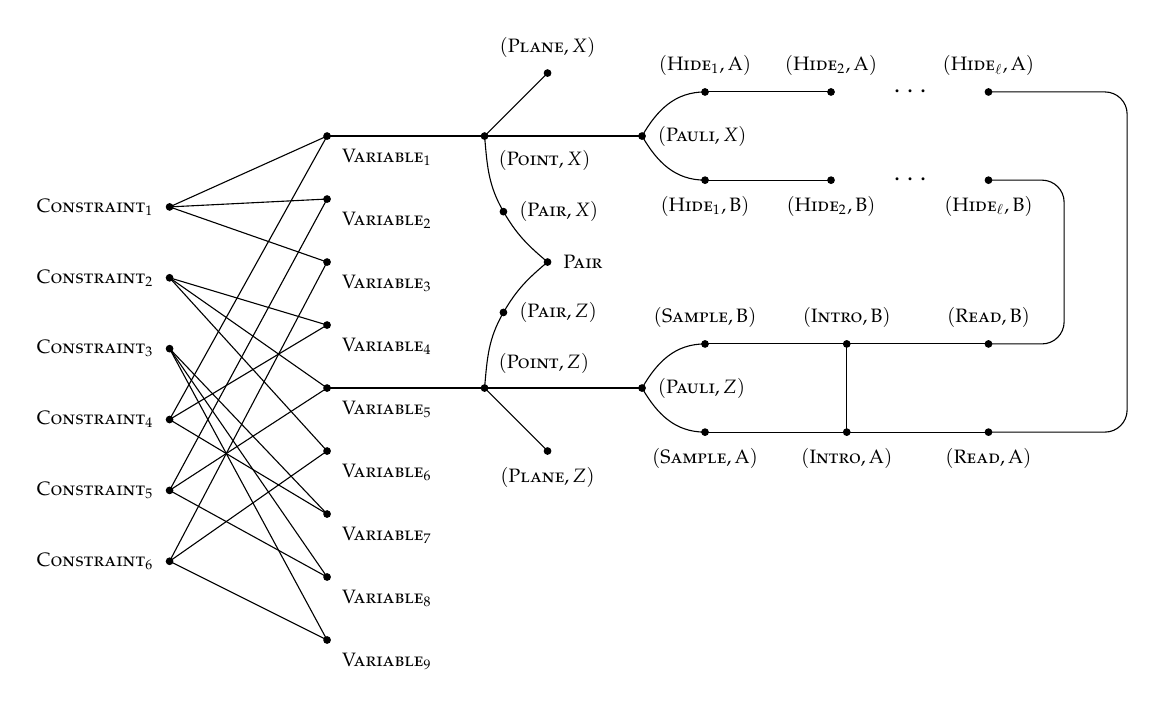
\begin{tikzpicture}[scale=.8]

    \tikzset{type/.style args={[#1]#2}{
        draw,circle,fill,scale=0.25,
        label={[font=\scriptsize, label distance=1pt]#1:#2}
      }}

    % Graph for MS

    \foreach \i in {1,...,6} \draw (0,8-9/8*\i)
    coordinate (Constraint-\i)
    node[type={[180]$\Constraint_\i$}] {};

    \foreach \i in {1,...,9} \draw (2.5,9-\i)
    coordinate (Variable-\i)
    node[type={[330]$\Variable_\i$}] {};

    \foreach \i in {1,...,3} \foreach \j in {1,...,3}
    \pgfmathsetmacro{\k}{(\i-1)*3+\j}
    \draw (Constraint-\i) -- (Variable-\k);

    \foreach \i in {4,...,6} \foreach \j in {1,...,3}
    \pgfmathsetmacro{\k}{\i-3+(\j-1)*3}
    \draw (Constraint-\i) -- (Variable-\k);

    % Types for QLD

    \draw (6,9) coordinate (Plane-X) node[type={[90]$(\Plane, X)$}] {};
    \draw (5,8) coordinate (Point-X) node[type={[315]$(\Point, X)$}] {};
    \draw (7.5,8) coordinate (Pauli-X) node[type={[0]$(\Pauli, X)$}] {};
    \draw (6,3) coordinate (Plane-Z) node[type={[270]$(\Plane, Z)$}] {};
    \draw (5,4) coordinate (Point-Z) node[type={[45]$(\Point, Z)$}] {};
    \draw (7.5,4) coordinate (Pauli-Z) node[type={[0]$(\Pauli, Z)$}] {};
    \draw (6,6) coordinate (Pair) node[type={[0]$\Pair$}] {};
    \draw (5.3,6.8) coordinate (Pair-X) node[type={[0]$(\Pair,X)$}] {};
    \draw (5.3,5.2) coordinate (Pair-Z) node[type={[0]$(\Pair,Z)$}] {};

    % Types for Intro

    \draw (8.5,8.7) coordinate (Hide-1-A) node[type={[90]$(\Hide{1}, \alice)$}] {};
    \draw (10.5,8.7) coordinate (Hide-2-A) node[type={[90]$(\Hide{2}, \alice)$}] {};
    \draw (11.8,8.7) node {$\cdots$};
    \draw (13,8.7) coordinate (Hide-l-A) node[type={[90]$(\Hide{\ell}, \alice)$}] {};

    \draw (8.5,7.3) coordinate (Hide-1-B) node[type={[270]$(\Hide{1}, \bob)$}] {};
    \draw (10.5,7.3) coordinate (Hide-2-B) node[type={[270]$(\Hide{2}, \bob)$}] {};
    \draw (11.8,7.3) node {$\cdots$};
    \draw (13,7.3) coordinate (Hide-l-B) node[type={[270]$(\Hide{\ell}, \bob)$}] {};

    \draw (8.5,3.3) coordinate (Sample-A) node[type={[270]$(\Sample, \alice)$}] {};
    \draw (10.75,3.3) coordinate (Intro-A) node[type={[270]$(\Introspect, \alice)$}] {};
    \draw (13,3.3) coordinate (Read-A) node[type={[270]$(\Read, \alice)$}] {};

    \draw (8.5,4.7) coordinate (Sample-B) node[type={[90]$(\Sample, \bob)$}] {};
    \draw (10.75,4.7) coordinate (Intro-B) node[type={[90]$(\Introspect, \bob)$}] {};
    \draw (13,4.7) coordinate (Read-B) node[type={[90]$(\Read, \bob)$}] {};

    % Edges

    \foreach \from/\to in {Plane-X/Point-X, Point-X/Pauli-X,
      Plane-Z/Point-Z, Point-Z/Pauli-Z,
      Point-X/Variable-1, Point-Z/Variable-5,
      Hide-2-A/Hide-1-A,
      Hide-2-B/Hide-1-B,
      Sample-A/Intro-A, Intro-A/Read-A,
      Sample-B/Intro-B, Intro-B/Read-B,
      Intro-A/Intro-B}
    \draw (\from) -- (\to);

    \draw (Pauli-X) to [out=60,in=180] (Hide-1-A);
    \draw (Pauli-X) to [out=300,in=180] (Hide-1-B);
    \draw (Pauli-Z) to [out=60,in=180] (Sample-B);
    \draw (Pauli-Z) to [out=300,in=180] (Sample-A);
    \draw [rounded corners=8] (Hide-l-A) to +(2.2,0) to +(2.2,-5.4) to (Read-A);
    \draw [rounded corners=8] (Hide-l-B) to +(1.2,0) to +(1.2,-2.6) to (Read-B);
    \draw (Point-X) to [out=275,in=120] (Pair-X) to [out=300,in=140] (Pair);
    \draw (Point-Z) to [out=85,in=240] (Pair-Z) to [out=60,in=220] (Pair);

  \end{tikzpicture}
  \caption{Type graph $G^\intro$ for the introspection game.
    Each vertex also has a self-loop which is not drawn in the figure for
    clarity.}
  \label{fig:type-graph-intro}
\end{figure}

\paragraph{Sampler.}
We first define a $2$-level $(\type^\intro,G^\intro)$-typed sampler
$\tilde{\sampler}^\intro$, which has field size $q(n)$ and dimension $4m(n) +
2$, where $q(n)$ and $m(n)$ are specified by $\introparams(r)$.
Note that the dimension is the same as that of the ambient space of the CL
functions of the Pauli basis test for $r$ qubits, specified in Section~\ref{sec:qld-cl-funcs}.

Fix $n \in \N$.
We specify the CL functions of $\tilde{\sampler}^\intro$ on index $n$.
Since the functions $L_{\hat{\tvar}}^{\alice,\, n}$ and
$L_{\hat{\tvar}}^{\bob,\, n}$ are identical for all $n$ and $\hat{\tvar}$, we
omit the superscripts $\alice$ and $\bob$.
For types $\hat{\tvar} \in \type^\pauli$, the CL functions $L_{\hat{\tvar}}^n$
are given by those specified in Section~\ref{sec:qld-cl-funcs}, parameterized by
$\introparams(r)$.
For types $\hat{\tvar} \in \type^\intro \setminus \type^\pauli$, the associated
CL functions are defined to be $0$-level CL functions (i.e., they are the $0$
map).
This means that for question types such as $\hat{\tvar}=(\Introspect, \trole)$
or $\hat{\tvar}=(\Sample, \trole)$ for $\trole\in\{\alice,\bob\}$ the associated question is solely comprised
of the question type label.

Finally, we define the typed sampler $\sampler^\intro$ to be
$\downsize(\tilde{\sampler}^\intro)$, the downsized sampler
(\cref{def:downsize-typed-sampler}) corresponding to $\tilde{\sampler}^\intro$.
By Lemma~\ref{lem:pauli-basis-sampler} the typed CL functions associated with
the Pauli basis test are $2$-level; using \cref{rk:higher-level,lem:cl-downsize}
it follows that $\sampler^\intro$ is a $2$-level typed sampler.

The following lemma establishes the complexity of the sampler $\sampler^\intro$
as well as the complexity of computing a {description} of it from the parameters
$(\lambda,\ell)$.
\begin{lemma}
  \label{lem:intro-sampler-complexity}
  There exists a $2$-input Turing machine $\ComputeIntroSampler$ that
  on input $(\lambda,\ell)$ outputs a description of the sampler
  $\sampler^\intro$ in time $\polylog(\lambda,\ell)$.
  Furthermore, 
  \begin{enumerate}
  \item $\TIME_{\sampler^\intro}(n) = \polylog((\lambda 2^n)^\lambda, \ell)$,
	\item $\RAND_{\sampler^\intro}(n) = \polylog((\lambda 2^n)^\lambda)$, and 
	\item $\sampler^\intro$  is a $2$-level typed sampler.
  \end{enumerate}
\end{lemma}

\begin{proof}
  Define the following $9$-input Turing machine
  $\hat{\cal{S}}^\intro$, that does not depend on any parameters (so that its description length is constant). 
  On input $(\lambda, \ell, n, x_1, \ldots, x_6)$, $\hat{\cal{S}}^\intro$
  computes the output of the typed sampler $\sampler^\intro$ (parameterized by
  $(\lambda, \ell)$) with input tapes set to $(n, x_1, \ldots, x_6)$.
  In more detail, the Turing machine $\hat{\cal{S}}^\intro$ first computes
  $\introparams(r)$ for $r=(\lambda N)^\lambda$ and $N=2^n$.
  Using \cref{lem:introparams-complexity}, this computation takes time
  $\poly\log(r)$.
  Next, depending on the contents of the last $7$ input tapes of
  $\hat{\cal{S}}^\intro$, the Turing machine evaluates the dimension of
  $\sampler^\intro$ (which can easily be computed from $\introparams(r)$), or
  one of the CL functions, or returns a representation of a factor space of
  $\sampler^\intro$.
  If the type passed as input is $\hat{\tvar} \in \type^\pauli$ then by
  Lemma~\ref{lem:qld-complexity} this takes time $\polylog(r)$.
  If $\hat{\tvar} \in \type^\intro\backslash\type^\pauli$ then this can be done
  in $O(\log \ell)$ time (to read the input type).
  Overall, $\hat{\cal{S}}^\intro$ runs in time $\poly\log(r,\ell)$.
  
  We now define the Turing machine $\ComputeIntroSampler$: on input
  $(\lambda,\ell)$, it outputs the description of $\hat{\cal{S}}^\intro$ with
  the first two input tapes hardwired to $\lambda$ and $\ell$, respectively,
  yielding the sampler $\sampler^\intro$ corresponding to parameters
  $(\lambda,\ell)$.
  Computing this description takes $O(\log \lambda + \log \ell)$ time.
  
  The time complexity of $\sampler^\intro$ follows from the time complexity of
  $\hat{\cal{S}}^\intro$, the randomness complexity follows from the dimension
  of the ambient space $4m(n) + 2 = \polylog(r)$, and the number of levels is by
  construction.
\end{proof}

\paragraph{Decider.}
The typed decider $\decider^\intro$ is specified in
Figure~\ref{fig:intro-decider}.
We explain how to interpret the figure, including the notation.
(It may also be helpful to review the description of the intended strategy for
the players in the game, described in Section~\ref{sec:comp-compl-intro}.)

\begin{figure}[!htbp]
  \begin{gamespec}
    \begin{table}[H]
      \centering
      \small
      \begin{tabularx}{.7\textwidth}{l X}
        \toprule
        Type \hspace{6em} & Answer format\\
        \midrule
        $(\Introspect, \trole)$ & $(y,a) \in V \times \{0,1\}^*$ \\
        $(\Sample, \trole)$ &  $(z,a) \in V \times \{0,1\}^*$ \\
        $(\Read, \trole)$ & $(y,y^{\perp},a) \in V \times V \times \{0,1\}^*$\\
        $(\Hide{k}, \trole)$ & $(y,y^{\perp},x) \in V \times V \times V$\\
        \bottomrule
      \end{tabularx}
    \end{table}
    In the following, whenever $\sampler$ or $\decider$ is called,
    $\decider^\intro$ aborts and rejects if the computation takes more than
    $(\lambda N)^\lambda$ time steps.
    On input $(n, \hat{\tvar}_\alice, \hat{x}_\alice, \hat{\tvar}_\bob,
    \hat{x}_\bob, \hat{a}_\alice, \hat{a}_\bob)$, the decider $\decider^\intro$
    first computes the dimension $s(N)$ of $V$ by calling the original sampler
    $\sampler$ on input $(N,\gamestyle{dimension})$.
    If $s(N) > (\lambda N)^\lambda$ the decider rejects.
    The decider then performs an answer length check: if
    \begin{equation}\label{eq:a-length-bound}
      \max \{ |\hat{a}_\alice|, |\hat{a}_\bob| \} \geq
      6s(N) + 2(\lambda N)^\lambda+3\;,
    \end{equation}
    then the decider rejects.
    Otherwise, it performs the following tests for all $w,\trole \in \AB$.
    (If no test applies, the decider accepts.) 
    
    \begin{enumerate}[itemsep=2pt, parsep=2pt]
    \item (\textbf{Pauli test}).
      \label{enu:pauli}
      If $\hat{\tvar}_\alice, \hat{\tvar}_\bob \in \type^\pauli$, accept if
      $\decider^\pauli_\introparams$ accepts the input $(\hat{\tvar}_\alice,
      \hat{x}_\alice, \hat{\tvar}_\bob, \hat{x}_\bob, \hat{a}_\alice,
      \hat{a}_\bob)$.
    \item (\textbf{Sampling tests}).
      \label{enu:sampling}
      \begin{enumerate}
      \item If $\hat{\tvar}_w = (\Pauli,Z)$ and $\hat{\tvar}_{\overline{w}} =
        (\Sample, \trole)$, accept if $\hat{a}_w^V = z_{\overline{w}}$.
        \label{enu:sampling-pauli}

      \item If $\hat{\tvar}_w = (\Introspect, \trole)$,
        $\hat{\tvar}_{\overline{w}} = (\Sample, \trole)$, accept if $y_{w} =
        L^\trole(z_{\overline{w}})$ and $a_w=a_{\overline{w}}$.
        \label{enu:sampling-intro}
      \end{enumerate}

    \item (\textbf{Hiding tests}).
      \label{enu:hiding}
      \begin{enumerate}

      \item If $\hat{\tvar}_w = (\Introspect, \trole)$,
        $\hat{\tvar}_{\overline{w}} = (\Read, \trole)$, accept if $y_{w} =
        y_{\overline{w}}$ and $a_w = a_{\overline{w}}$.
        \label{enu:hiding-intro}

      \item If $\hat{\tvar}_w = (\Hide{\ell}, \trole)$,
        $\hat{\tvar}_{\overline{w}} = (\Read, \trole)$, accept if $y_{w,\,
          <\ell} = y_{\overline{w},\, <\ell}$, and $y^{\perp}_w =
        y^{\perp}_{\overline{w}}$.
        \label{enu:hiding-read}
        
      \item \label{enu:hiding-same} If $\hat{\tvar}_w = (\Hide{k}, \trole)$,
        $\hat{\tvar}_{\overline{w}} = (\Hide{k+1}, \trole)$ for some $k \in \{ 1,
        2, \ldots, \ell-1 \}$, accept if
        \begin{equation*}
          y_{w,\, <k} = y_{\overline{w},\, <k}\;, \quad
          y^{\perp}_{w,\, \le k} = y^{\perp}_{\overline{w},\, \le k}\;, \quad
          x_{w,\, >k+1} = x_{\overline{w},\, >k+1}\;,
        \end{equation*}
        and $y^{\perp}_{\overline{w},\, k+1} = \big( L^{\trole}_{k+1,\, u} \big)^\perp
        (x_{w,\, k+1})$ where $u = y_{\overline{w},\, \le k}$.
      \item If $\hat{\tvar}_w = (\Pauli,X)$, $\hat{\tvar}_{\overline{w}} =
        (\Hide{1}, \trole)$, accept if $y^\perp_{\overline{w},\, 1} =
        \bigl( L^{\trole}_1 \bigr)^\perp (\hat{a}_w^{V_1})$ and $\hat{a}_w^{V_{> 1}} =
        x_{\overline{w},\, >1}$.
        \label{enu:hiding-pauli}
      \end{enumerate}

    \item (\textbf{Game test}).
      \label{enu:intro-game}
      If $\hat{\tvar}_w = (\Introspect, \alice)$ and $\hat{\tvar}_{\overline{w}}
      = (\Introspect, \bob)$, accept if $\decider$ accepts $(N, y_w,
      y_{\overline{w}}, a_w, a_{\overline{w}})$ for $N = 2^n$.

    \item (\textbf{Consistency test}).
      \label{enu:intro-consistency}
      If $\hat{\tvar}_\alice = \hat{\tvar}_\bob$, accept if and only if
      $\hat{a}_\alice = \hat{a}_\bob$.
    \end{enumerate}
  \end{gamespec}
  \caption{The typed decider $\decider^\intro$ for the introspective verifier,
    parameterized by integers $\lambda, \ell$, on index $n$.
    $N$ denotes $2^n$, $V$ is the ambient space for $\sampler$, and
    $\{L^\trole\}_{\trole\in\{\alice,\bob\}}$ the associated CL functions on
    index $N$.}
  \label{fig:intro-decider}
\end{figure}

\medskip
\emph{Question and answer format.}
The decider takes as input a tuple $(n, \hat{\tvar}_\alice, \hat{x}_\alice,
\hat{\tvar}_\bob, \hat{x}_\bob, \hat{a}_\alice, \hat{a}_\bob)$ where
$(\hat{\tvar}_w,\hat{x}_w)$ denotes the question for introspecting player $w \in
\AB$, and $\hat{a}_w$ denotes their answer.
As in the specification of the Pauli basis test, in
Figure~\ref{fig:intro-decider} we include an ``answer key'' indicating how the
players' answers are parsed, depending on the question type.
When the question type is from $\type^\pauli$, the question and answer format
are as described in Figure~\ref{fig:decider_pauli}.
When the question type is in $\type^\intro \setminus \type^\pauli$, the answer
format is described in the table at the top of
Figure~\ref{fig:intro-decider}.\footnote{There is no question format
  specification for the question types in $\type^\intro \setminus \type^\pauli$,
  because the question is solely comprised of the question type label.}
For each such question, there is an associated variable $\trole \in \AB$ that
indicates to the introspecting player which {original player} it is supposed to
impersonate in the introspection game.

In the figure, $V$ denotes the ambient space of the original sampler $\sampler$
on index $N = 2^n$.
Since $V$ is isomorphic to $\F_2^{s(N)}$, where $s(N)$ is the dimension of
$\sampler$, the space $V$ is identified in a canonical way as the register
subspace of $\F_2^r$ spanned by $e_1,\ldots,e_{s(N)}$ where $e_i$ is the $i$-th
elementary basis vector.
For example, if $\hat{\tvar}_w = (\Read,\trole)$, then syntactically the
player's answer is a triple $(y,y^\perp,a)$ in $\F_2^r \times \F_2^r
\times \{0,1\}^*$.
We assume that the decider $\decider$ computes the dimension $s(N)$ of the
subspace $V$ by calling $\sampler$ on input $(N,\gamestyle{dimension})$, and
 if $y,y^\perp$ are not presented as vectors in the subspace $V$,
then the decider rejects. Thus in the analysis we directly consider $y,y^\perp$ as vectors in $V$.
In \Cref{fig:intro-decider}, the components of the players' answers are
subscripted by the player index.
For example, if player $w$ receives question $(\Hide{k},\trole)$, then their
answers are denoted by $(y_w,y_w^\perp,x_w)$.

The notation used in the ``answer key'' is meant to give an indication of the
intended meaning of the players' answers.
We use $y$ to denote a vector that is supposed to be the result of measuring a
CL function $L^\trole$; $y^\perp$ is supposed to be the result of measuring
``dual'' linear maps $L^\perp$ (as used in Step~\ref{enu:hiding} in
Figure~\ref{fig:intro-decider}); $x$ is supposed to be the result of $\sigma^X$
measurements, and $z$ is supposed to be the result of $\sigma^Z$ measurements.
We use $a$ to denote the introspected answers meant for the original decider
$\decider$.

\medskip
\emph{CL functions and factor spaces.}
For $\trole \in \AB$, let $L^\trole = L^{\trole,\, N}$ denote the CL function
for original player $\trole$ specified by $\sampler$ on index $N = 2^n$.
For $z \in V$, the decider $\decider$ computes $L^\trole(z)$ by calling
$\sampler$ on input $(N, \trole, \gamestyle{marginal}, \ell, z)$.

For $y \in V$ and $k \in \{1,\ldots,\ell\}$ we define register subspaces
$V_{k}^\trole (y)$ by induction on $k$.
For $k=1$, $V_1^\trole(y)$ is the first factor space\footnote{See
  Lemma~\ref{lem:cl-kth} for the definitions of factor spaces of a CL function.}
of $L^\trole$ and is independent of $y$.
Suppose $V_j^\trole(y)$ has been defined for all $j < k$.
Then we define the marginal space $V_{< k}^\trole(y) = \bigoplus_{j=1}^{k-1}
V_k^\trole(y)$, and define $V_k^\trole(y)$ as the $k$-th factor space $V_{k,\,
  u}^\trole$ of $L^\trole$ with prefix $u = y^{V_{<k}^\trole(y)}$, the
projection of $y$ to $V_{<k}^\trole(y)$.
We also define $V^\trole_{\leq k}(y) = V^\trole_{< k+1}(y)$, and $V^\trole_{>
  k}(y)$ to be the complementary register subspace to $V^\trole_{\leq k}(y)$
within $V$.

The decider $\decider^\intro$ computes factor spaces $V_j^\trole(y)$ from $y \in
V$ in the following sequential manner: first, the indicator vector for the
factor space $V^\trole_1$ is computed by calling the original sampler $\sampler$
on input $(N,\trole,\gamestyle{factor},1,0)$.
Let $y_1$ denote the projection of $y$ to $V^\trole_1$.
Then, for $j \in \{2,\ldots,\ell\}$, the factor space $V^\trole_j(y)$ is
computed by calling $\sampler$ on input $(N,\trole,\gamestyle{factor},j,y_{\le
  j-1})$, where $y_{\le j-1}$ is the projection of $y$ to $V^\trole_{\le
  j-1}(y)$.

We give more details on the implementation of decider $\decider^\intro$
specified in Figure~\ref{fig:intro-decider}.

\begin{enumerate}
\item The decider $\decider^\intro$ first checks that the answers are not too
  long; the maximum length answer should be either a tuple $(y, y^\perp, a)$ where
  $y, y^\perp \in V$ and $a$ is an answer intended for the original decider
  $\decider$ on index $N$ (which we assume runs in time at most $(\lambda
  N)^\lambda$), or a tuple $(y,y^\perp,x) \in V \times V \times V$.
  This check is necessary in order to ensure that the decider $\decider^\intro$
  halts in time $\poly(N)$.
  The bound~\eqref{eq:a-length-bound} is explained by the encoding for
  tuples specified in Remark~\ref{rmk:tm-representations}.

\item If the question types for the players are both in $\type^\pauli$,
  $\decider^\intro$ executes the decision procedure $\decider^\pauli$ for the
  Pauli basis test parametrized by $\introparams$ (see
  Section~\ref{sec:qld-game} for the definition of $\decider^\pauli$).
  The Pauli basis test is intended to ensure that the players share an $r$-qubit
  EPR state, where $r = (\lambda N)^\lambda$.
  Since the EPR state is measured to introspectively sample questions according
  to the original sampler $\sampler$, it is necessary that $r$ is at least as
  large as the randomness complexity of $\sampler$, which is equal to the
  dimension of $\sampler$ (since for a normal form verifier the field size is
  taken to be $q(n) = 2$).
  This is satisfied under the assumption stated
  in~\eqref{eq:intro-complexity-assump}.

\item In Step~\ref{enu:sampling-pauli} of $\decider^\intro$, player
  $w\in\{\alice,\bob\}$ receives question $(\Pauli,Z)$ and player $\overline{w}$
  receives question $(\Sample,\trole)$, for some $v\in\{\alice,\bob\}$.
  According to the answer key, player $w$ is expected to return an answer
  $\hat{a}_w\in \F_2^r$ and player $\overline{w}$ is expected to respond with a
  pair $(y_{\overline{w}},a_{\overline{w}}) \in V \times \{0,1\}^*$.
  Thus, the dimension of answer $\hat{a}_w$ may be larger than that of
  $y_{\overline{w}}$; this is the reason that Step~\ref{enu:sampling-pauli}
  checks consistency between $y_{\overline{w}}$ and the projection of
  $\hat{a}_w$ to $V$.



\item In Step~\ref{enu:sampling-intro} of $\decider^\intro$, player $w \in \ab$
  receives question $(\Introspect,\trole)$ and player $\overline{w}$ receives
  question $(\Sample,\trole)$.
  As specified by the ``answer key'', player $w$ responds with $(y_w,a_w) \in V
  \times \{0,1\}^*$ and player $\overline{w}$ responds with
  $(z_{\overline{w}},a_{\overline{w}}) \in V \times \{0,1\}^*$.
  The decider $\decider^\intro$ checks that $a_w = a_{\overline{w}}$ and $y_w =
  L^\trole(z_{\overline{w}})$ where $L^\trole$ denotes the CL function for
  player $\trole$ specified by $\sampler$ for index $N = 2^n$.
  The CL function is computed by calling $\sampler$ on input
  $(N, \trole, \gamestyle{marginal}, \ell, z)$.

\item In Step~\ref{enu:hiding-read}, $\decider^\intro$ checks that the answer of
  player $w$ who received $(\Hide{\ell},\trole)$ is consistent with the answer
  of player $\overline{w}$ who received $(\Read,\trole)$. One of the checks is
  that $y_{w,< \ell} = y_{\overline{w},<\ell}$\;; these are, respectively, the
  projections of $y_w$ to $V^\trole_{< \ell}(y_w)$ and $y_{\overline{w}}$ to
  $V^\trole_{< \ell}(y_{\overline{w}})$.

\item\label{enu:decider-perp}
  \def\Lfunc{L^{\trole}_{k+1,\, y_{\overline{w},\, \le k}}}

  In Steps~\ref{enu:hiding-same}, the vectors $x_{w,\, >k+1}$ and
  $x_{\overline{w},\, >k+1}$ denote the projections of $x_w$ and
  $x_{\overline{w}}$ to $V^\trole_{> k+1}(y_w)$ and $V^\trole_{>
    k+1}(y_{\overline{w}})$, respectively.
  Similarly, $y_{\overline{w},\, k+1}^\perp$ denotes the projection of
  $y_{\overline{w}}^\perp$ to $V^\trole_{k+1} (y_{\overline{w}})$ and
  $x_{w,\, k+1}$ denotes the projection of $x_{w}$ to
  $V^\trole_{k+1}(y_{\overline{w}})$.
  Note that the factor spaces depend on $y_w$ and $y_{\overline{w}}$.

  The decider also has to compute $( \Lfunc )^\perp (x_{w,\, k+1})$.
  According to Definition~\ref{def:Lperp}, this requires specifying a basis for
  $\ker( \Lfunc )^\perp$.
  To compute the value, the decider performs the following steps:
	\begin{enumerate}
  \item Call $\sampler$ on input $(N, \trole, \gamestyle{factor}, k+1, y_{w,\, \le k})$ to
    obtain a subset $H = \{h_1,\ldots,h_m\}$ of the canonical basis for
    $\F_2^{s(N)}$ that is a basis of the register subspace $V^\trole_{k+1}(y_{\overline{w}})$.
  \item For $i \in \{1, 2, \ldots, m\}$ compute $c_i = \sampler(N, \trole,
    \gamestyle{linear}, k+1, y_{\overline{w},\, \le k}, h_i)$.
    Compute a matrix representation $M$ for $ \Lfunc $ in the basis
    $H$, whose columns are the vectors $c_1, \ldots, c_m$ as elements of
    $V^\trole_{k+1}(y_{\overline{w}})$.

  \item Using a canonical algorithm for Gaussian elimination, compute a basis
    $F$ for $\ker(M)$.

  \item Compute the canonical complement $S$ of $F$, as in
    Definition~\ref{def:canonical-complement}.
    $S$ is a basis for $\ker( \Lfunc )^\perp$.

  \item To compute $(\Lfunc)^\perp$ on input
    $x_{w,\, k+1}$, compute the canonical linear map with kernel basis
    $S$ (see Definition~\ref{def:cl-canonical}) on input $x_{w,\,
      k+1}$.
  \end{enumerate}

\item In Step~\ref{enu:hiding-pauli}, the player $w$ that receives $(\Pauli,X)$
  is expected to return an answer $\hat{a}_w$ in $\F_2^r$.
  Part of this step checks that the projection of $\hat{a}_w$ to $V_{>1}$ is
  equal to $x_{\overline{w},\, >1}$ (which is the projection to $V_{>1}$ of the
  third component of the answer triple of player $\overline{w}$ that receives
  question $(\Hide{1},\trole)$).

\end{enumerate}

The following lemma establishes the complexity of the decider $\decider^\intro$
as well as the complexity of computing a {description} of it from the parameters
$(\lambda,\ell)$ and the description of the original verifier $\verifier =
(\sampler,\decider)$.

\begin{lemma}
  \label{lem:intro-decider-complexity}
  There exists a $4$-input Turing machine $\ComputeIntroDecider$ that
  on input $(\verifier,\lambda,\ell)$ outputs a description of the decider
  $\decider^\intro$ in time $\poly(\abs{\verifier}, \log\lambda, \log\ell)$.
  Furthermore, the decider $\decider^\intro$ has time complexity
  $\TIME_{\decider^\intro}(n) = \poly((\lambda 2^n)^\lambda, \ell)$.
\end{lemma}

\begin{proof}
  Define the following $10$-input Turing machine $\hat{\cal{D}}^\intro$.
  The Turing machine does not depend on any parameters, so its size is constant.
  On input
  \begin{equation*}
    (\verifier, \lambda, \ell, n, x_1, x_2, \ldots, x_6),
  \end{equation*}
  $\hat{\cal{D}}^\intro$ computes the output of the decider $\decider^\intro$
  with input tapes set to $(n,x_1,\ldots,x_6)$.
  In more detail, the Turing machine $\hat{\cal{D}}^{\intro}$ first computes
  $\introparams(r)$ for $r=(\lambda N)^\lambda$ and $N=2^n$.
  Using Lemma~\ref{lem:introparams-complexity}, this computation takes time
  $\polylog(r)$.
  It then executes the tests described in Figure~\ref{fig:intro-decider}.
  Write $\verifier = (\sampler, \decider)$.
  The complexity of performing the entire procedure is subsumed by the
  complexity of the following steps:
	\begin{enumerate}
  \item Running the decider $\decider^\pauli$, which takes time $\poly(r)$ by
    Lemma~\ref{lem:qld-complexity};
  \item Running the original decider $\decider$ (on index $N = 2^n$) for at most
    $(\lambda N)^\lambda$ steps;
  \item Running the original sampler $\sampler$ (on index $N$) in order to
    compute the dimension $s(N)$ and the marginal and factor spaces, and the CL
    functions as described in Section~\ref{sec:intro-verifier}.
    $\sampler$ is called at most $\poly(s(N),\ell)$ times; due to the timeout,
    each call takes time at most $(\lambda N)^\lambda$.
  \item Computing $(L^\trole_{k,\, u})^\perp(x_{\overline{w},\, k})$ in
    Step~\ref{enu:hiding-same}.
    This only requires to perform Gaussian elimination and other simple finite
    field manipulations that can be implemented in $\poly(s(N), \log \abs{\F})$
    time.
	\end{enumerate}
  All other tests are elementary.
  Thus the time complexity of $\hat{\cal{D}}^\intro$ is $\poly(r,\ell)$.
  Note that the bound is independent of $\verifier$: due to the abort
  condition in the definition of $\decider^\intro$, the Turing machine
  $\hat{\decider}^\intro$ aborts if the runtime of $\sampler$ or $\decider$ is
  larger than $(\lambda N)^\lambda$.

  We now define the Turing machine $\ComputeIntroDecider$: on input
  $(\verifier,\lambda,\ell)$, it outputs the description of
  $\hat{\cal{D}}^\intro$ with the first three input tapes hardwired to
  $\verifier$, $\lambda$, and $\ell$, respectively, yielding the decider
  $\decider^\intro$ corresponding to original verifier $\verifier$ and
  parameters $(\lambda, \ell)$.
  Computing this description takes $\poly(\abs{\verifier}, \log\lambda, \log
  \ell)$ time.
  The time complexity of $\decider^\intro$ follows from the time complexity of
  $\hat{\cal{D}}^\intro$.
\end{proof}

\subsection{Completeness and complexity of the introspective verifier}

In this section we determine the complexity of the introspective verifier and
establish the completeness property of the introspection game: if for $N = 2^n$,
$\verifier_N$ has a PCC strategy (see Definition~\ref{def:spcc})  with value $1$,
then so does $\verifier^\intro_n$.
For this we describe the actions that are expected of the players in the
introspection game (i.e.\ the ``honest strategy'').
We first prove several preliminary lemmas that will be used in both the
completeness and soundness analysis.

\subsubsection{Preliminary lemmas}

The lemmas in this section are stated for general fields $\F$ and generalized
Pauli observables and projectors, although in the application to introspection
games we use $\F = \F_2$, $\omega = -1$, and qubit Pauli observables and
projectors.
Furthermore, the Pauli observables $\tau^W(v)$ and projectors $\tau^W_u$ act on
$\C^{\F^k}$ for some integer $k$ (in our application, we set $k=r$).

\begin{lemma}[Fact 3.2 of \cite{NW19}]
  \label{lem:cancellation}
  Let $V$ be a subspace of $\F^k$. For all $v \not\in V^\perp$, 
  \begin{equation*}
    \E_{u \sim V} \omega^{\tr(u \cdot v)} = 0\;,
  \end{equation*}
  where the expectation is over a uniformly random vector $u$ from $V$.
\end{lemma}


The next lemma generalizes Eq.~\eqref{eq:pauli-inversion-0}.

\begin{lemma}\label{lem:why-didnt-i-think-of-this-before}
Let $L: \F^k \to \F^k$ be a linear map, and let $W \in \{X, Z\}$.
For each $a$ in the range of $L$, let $u_a \in \F^k$ be such that $L(u_a) = a$. 
\begin{enumerate}
\item For each $v \in \ker(L)^\perp$, 
\begin{equation*}
\tau^W(v) = \sum_{a \in \F^k} \omega^{\tr(u_a \cdot v)} \tau^W_{[L(\cdot)=a]}\;.
\end{equation*}
\item For all $a$ in the range of $L$,
\begin{equation*}
\tau^W_{[L(\cdot)=a]} = \E_{v \sim \ker(L)^\perp} \omega^{-\tr(v \cdot u_a)} \tau^W(v)\;.
\end{equation*}
\end{enumerate}
\end{lemma}

\begin{proof}
  Let $V$ denote the image of $\F^k$ under $L$.
  Let $a\in V$, $v \in \ker(L)^\perp$.
  For all $u, u' \in L^{-1}(a)$, we have that $u-u'\in \ker(L)$ and thus $\tr(u
  \cdot v) = \tr(u' \cdot v)$.
  As a result, using~\eqref{eq:pauli-obs-proj}, for any $v\in\ker(L)^\perp$ it
  holds that
  \begin{equation*}
    \tau^W(v)
    = \sum_{u \in \F^k} \omega^{\tr(u \cdot v)} \tau^W_u
    = \sum_{a \in V} \sum_{u \in L^{-1}(a)} \omega^{\tr(u \cdot v)} \tau^W_u
    = \sum_{a \in V} \omega^{\tr(u_a \cdot v)} \tau^W_{[L(\cdot)=a]}
    = \sum_{a \in \F^k} \omega^{\tr(u_a \cdot v)} \tau^W_{[L(\cdot)=a]}\;,
  \end{equation*}
  where in the last equality we used that for $a \notin V$, the projector
  $\tau^W_{[L(\cdot)=a]}$ vanishes.
  This shows the first item.
  For the second item,
  \begin{align*}
    \tau^W_{[L(\cdot)=a]}
    & = \sum_{u  \in L^{-1}(a)} \tau^W_u\\
    & =  \sum_{u  \in L^{-1}(a)} \E_{v \sim \F^k} \Bigl(
      \omega^{-\tr(u \cdot v)} \tau^W(v) \Bigr) && \\
    & =  \sum_{u \in \ker(L)} \E_{v \sim \F^k} \Bigl(
      \omega^{-\tr((u_a + u) \cdot v)} \tau^W(v) \Bigr)\\
    & = \frac{|\ker(L)|}{|\F^k|} \sum_{v \in \F^k} \biggl( \Big(
      \E_{u \sim \ker(L)} \omega^{-\tr(u \cdot v)} \Big)\,
      \omega^{-\tr(u_a \cdot v)}  \tau^W(v) \biggr)\\
    & = \E_{v \in \ker(L)^\perp} \omega^{-\tr(v \cdot u_a)} \tau^W(v)\;,
\end{align*}
where the second equality follows from~\eqref{eq:pauli-inversion-0} and the last
uses the fact that $|\F^k|=|\ker(L)||\ker(L)^\perp|$, as shown in
Lemma~\ref{lem:perp_perp}, and Lemma~\ref{lem:cancellation} applied to the
expectation over~$u$.
\end{proof}


\begin{lemma}[Commuting~$X$ and~$Z$ measurements]
  \label{lem:commute} 
	For all linear maps $L,R: \F^k \to \F^k$ such that
  \begin{equation*}
    \ker (R)^\perp \subseteq \ker (L)\;,
  \end{equation*}
  the measurements
  $\big\{ \tau^Z_{[L(\cdot)=b]} \big\}_{b\in \F^k}$ and $\big\{ \tau^X_{[R(\cdot) = d]}
  \big\}_{d\in \F^k}$ commute.
\end{lemma}
\begin{proof}
  Let $b,d\in \F_k$.
  If either $b$ is not in the range of $L$, or $d$ is not in the range of $R$,
  then at least one of $\tau^Z_{[L(\cdot) = b]}$ or $\tau^X_{[R(\cdot) = d]}$ is
  $0$, and thus the operators trivially commute.
  Otherwise, both $b$ and $d$ are in the range of $L$ and $R$, respectively.
  Let $a_0 \in L^{-1}(b)$, $c_0 \in R^{-1}(d)$.
  By Lemma~\ref{lem:why-didnt-i-think-of-this-before},
  \begin{equation*}
    \tau^Z_{[L(\cdot)=b]} = \E_{u \in \ker(L)^\perp}
    \omega^{\tr(u \cdot a_0)} \tau^Z(u)\;,
  \end{equation*}
  \begin{equation*}
    \tau^X_{[R(\cdot)=d]} = \E_{v \in \ker(R)^\perp}
    \omega^{\tr(v \cdot c_0)} \tau^X(v)\;.
  \end{equation*}
  For any $v \in \ker(R)^\perp$, by assumption $v\in \ker(L)$, so for $u \in
  \ker(L)^\perp$ it holds that $u\cdot v=0$.
  Thus $\tau^Z(u)$ and $\tau^X(v)$ commute, and it follows that
  $\tau^Z_{[L(\cdot)=b]}$ and $\tau^X_{[R(\cdot)=d]}$ commute as well.
\end{proof}

\subsubsection{Complexity and completeness of the introspective verifier}
\label{sec:comp-compl-intro}

The following theorem formulates the complexity and completeness properties of
the introspective verifier.
Since $\verifier^\intro$ is a typed verifier, we use the detyping procedure
described in Section~\ref{sec:detype} to obtain an untyped normal form verifier.

\begin{theorem}[Complexity and completeness of the introspective verifier]
  \label{thm:intro-completeness}
  Let $\lambda,\ell \in \N$.
  Let $\verifier = (\sampler, \decider)$ be a normal form verifier such that
  $\sampler$ is an $\ell$-level sampler.
  Let $\verifier^\intro = (\sampler^\intro, \decider^\intro)$ be the typed
  introspective verifier corresponding to $\verifier$ and parameters
  $(\lambda,\ell)$.
  Let $\detype(\verifier^\intro) =
  (\detype(\sampler^\intro),\detype(\decider^\intro))$ denote the detyped
  verifier.

  \begin{enumerate}
  \item (\textbf{Completeness}) Suppose that $\verifier$ satisfies the
    assumption stated in~\eqref{eq:intro-complexity-assump}.
    Then for all $n \in \N$ and $N = 2^n$, if $\verifier_N$ has a projective,
    consistent, and commuting (PCC) strategy with value $1$ then
    $\detype(\verifier^\intro)_n$ also has a PCC strategy with value $1$.
  \item (\textbf{Sampler complexity}) The sampler $\sampler^\intro$ is a
    $(\type^\intro,G^\intro)$-type, $2$-level sampler.
    Moreover, the time and randomness complexities of $\detype(\sampler^\intro)$
    satisfy that for all $n\in \N$,
    \begin{gather*}
      \TIME_{\detype(\sampler^\intro)}(n) = \poly \big (\lambda\log (\lambda
      N),\ell \big)\;, \\
      \RAND_{\detype(\sampler^\intro)}(n) = \poly \big (\lambda\log (\lambda N)
      ,\ell\big)\;,
    \end{gather*}
    where $N = 2^n$.

  \item (\textbf{Decider complexity}) The time complexity of the decider
    $\decider^\intro$ satisfies that for all $n\in \N$,
    \[
      \TIME_{\detype(\decider^\intro)}(n) = \poly \big ((\lambda
      N)^\lambda,\ell\big)\;,
    \]
    where $N=2^n$.

  \item (\textbf{Efficient computability}) \label{enu:intro-computability} There
    is a Turing machine $\ComputeIntroVerifier$ which takes as input a tuple
    $(\verifier, \lambda, \ell)$ with $\lambda, \ell \in \N$ and returns
    the description of the detyped introspective verifier
    $\detype(\verifier^\intro) =
    (\detype(\sampler^\intro),\detype(\decider^\intro))$ corresponding to
    $\verifier$ and parameters $(\lambda,\ell)$ in time
    $\poly(\abs{\verifier}, \log \lambda, \log \ell)$.

  \end{enumerate}
\end{theorem}

\begin{proof} 
  We analyze the completeness and complexity properties of the \emph{typed}
  verifier $\verifier^\intro$; the corresponding properties of the
  \emph{detyped} verifier $\detype(\verifier^\intro)$ follow from
  Lemma~\ref{lem:detyping-verifiers}, and the fact that the type set
  $\type^\intro$ has size $O(\ell)$.

  \paragraph{Completeness.}
  We first show completeness.
  Let $n\geq 1$ be an index for $\verifier^\intro$ and $N = 2^n$ be the
  corresponding index for $\verifier$.
  The assumption on the time complexity of $\verifier$ ensures that
  $\decider^\intro$ never aborts due to a timeout.
	Let $L^\trole = L^{\trole,\, N}$ denote the CL function of the original
  sampler $\sampler$ on index $N$ corresponding to player $\trole \in \AB$.
  Let $r = (\lambda N)^\lambda$, and let $\introparams(r) =
  (q,m,d,h,H,\Gamma,\pi)$, as in Section~\ref{sec:intro-verifier}.
  Set $Q = \Gamma \log q$\,; this represents the number of qubits that are
  certified by the Pauli basis test parameterized by $\introparams(r)$.
  Let $\strategy = (\ket{\aux}, A, B)$ be a PCC strategy for $\verifier_N$ with
  value~$1$.
  We first construct a PCC strategy $\strategy^\intro_n$ for the typed verifier
  $\verifier^\intro_n$ with value $1$.
  We then conclude using Lemma~\ref{lem:detyping-verifiers}.

  \begin{figure}[htb!]
    \centering
    \begin{gamespec}
      \newcolumntype{M}{>{\arraybackslash $}X<{$}}
      \renewcommand{\arraystretch}{1.6}
      \begin{tabularx}{\textwidth}{*{6}M}
        \toprule
        & \phantom{I1} V^\trole_1
        & \phantom{I1} V^\trole_2 & \phantom{I1} V^\trole_3 & \aux \\
        \midrule
        (\Introspect, \trole) & \sigma^Z_{L_1} & \sigma^Z_{L_2} &
        \sigma^Z_{L_3} & A^x/B^x \\
        (\Sample, \trole) & \sigma^Z & \sigma^Z & \sigma^Z & A^x/B^x \\
        (\Read, \trole) & \sigma^Z_{L_1^{\phantom{\perp}}}\;
        \sigma^X_{L_1^\perp} &
        \sigma^Z_{L_2^{\phantom{\perp}}}\;
        \sigma^X_{L_2^\perp} &
        \sigma^Z_{L_3^{\phantom{\perp}}}\;
        \sigma^X_{L_3^\perp} & A^x/B^x \\
        \midrule
        (\Hide{3}, \trole) & \sigma^Z_{L_1^{\phantom{\perp}}}\;
        \sigma^X_{L_1^\perp} &
        \sigma^Z_{L_2^{\phantom{\perp}}}\;
        \sigma^X_{L_2^\perp} &
        \phantom{\sigma^Z_{L_3^{\phantom{\perp}}}\;}
        \sigma^X_{L_3^\perp} & I \\
        (\Hide{2}, \trole) & \sigma^Z_{L_1^{\phantom{\perp}}}\;
        \sigma^X_{L_1^\perp}
        & \phantom{\sigma^Z_{L_1^{\phantom{\perp}}}\;}
        \sigma^X_{L_2^\perp}
        & \sigma^X & I \\
        (\Hide{1}, \trole) & \phantom{\sigma^Z_{L_1^{\phantom{\perp}}}\;}
        \sigma^X_{L_1^\perp} & \sigma^X & \sigma^X & I \\
        \midrule
      \end{tabularx}
      The left-most column denotes the introspection/hiding questions that a
      player may receive.
      The top row denotes the registers corresponding to the factor spaces of a
      CL function $L^\trole$ (we note that the partition of the registers depends
      on the prefixes), as well as the register corresponding to the state
      $\ket{\aux}$ coming from the original PCC strategy $\strategy$.
      We use $\sigma^Z_{L_j}$ as shorthand for $\sigma^Z_{[ L^\trole_{j,\,
          x_{<j}} (\cdot) = x_j ]}$ and similarly $\sigma^X_{L^\perp_j}$ for $
      \sigma^X_{[ (L^\trole_{j,\, x_{<j}})^\perp (\cdot)=x_j^\perp]}$.
      A symbol $I$ means that the register is left unmeasured.
    \end{gamespec}
    \caption{Summary of the honest strategy $\strategy_n^\intro$ for
      $\verifier_n^\intro$ for a $3$-level sampler.}
    \label{fig:intro-honest}
  \end{figure}

  \begin{remark}
    \label{rk:downsizing}
    Note that by definition in $\verifier_n^\intro$ the players receive
    questions $(x,y)$ that are sampled according to the distribution
    $\mu_{\sampler^\intro,\, n}^{G^\intro}$ associated with the downsized typed
    sampler $\downsize(\tilde{\sampler}^\intro)$.
    Using the definition of the downsized typed sampler,
    Definition~\ref{def:downsize-typed-sampler}, and
    Lemma~\ref{lem:downsize-cl-dist} the distribution is identical to the
    distribution $\mu_{\tilde{\sampler}^\intro,\, n}^{G^\intro}$, up to the
    bijective mapping $\downsize$.
    This mapping can be computed by the players themselves.
    Therefore, we construct a strategy for players that receive questions from
    $\mu_{\tilde{\sampler}^\intro,\, n}^{G^\intro}$, and a strategy for
    questions from $\mu_{\sampler^\intro,\, n}^{G^\intro}$ follows immediately.
  \end{remark}

  The strategy $\strategy^\intro_n$ uses the state $\ket{\EPR_2}^{\otimes (Q+1)}
  \otimes \ket{\aux}$, where recall that $\ket{\EPR_2} =
  \frac{1}{\sqrt{2}}(\ket{00}+\ket{11})$.
  For all register subspaces $R \subseteq \F_2^{Q}$ (see
  Definition~\ref{def:cl-func} for the definition of register subspace),
  whenever we refer to ``register $R$'', we mean the qubits of
  $\ket{\EPR_2}^{\otimes Q}$ corresponding to $R$ (see
  Section~\ref{sec:lin-reg}).
  The most frequent register subspace we consider is~$V$, spanned by $e_1,
  \ldots, e_{s(N)}$.
  We write $\overline{V}$ for the complement of~$V$, i.e.
  the register subspace spanned by $e_{s(N)+1}, \ldots, e_{Q}$.
  (Note that $s(N) \leq r \leq Q$ by
  assumption~\eqref{eq:intro-complexity-assump} and the definition of $Q$.)
  Then $\ket{\EPR_2}^{\otimes Q} = \ket{\EPR}_V \otimes
  \ket{\EPR}_{\overline{V}}$.

  Let $\strategy^\bp_n$ be the honest binary Pauli strategy with respect to
  $\introparams$ defined in the proof of \cref{lem:pauli-completeness}.
  For a question of type in $\type^\pauli$ the player measures the shared state
  $\ket{\EPR_2}^{\otimes (Q+1)}$ using the measurements specified by
  $\strategy^\bp_n$, and reports the measurement outcomes.
  When a player receives questions of type $\hat{\tvar} \in \type^\intro
  \setminus \type^\pauli$, they perform measurements described as follows.
  (Below, whenever we write a Pauli operator $\sigma^W_a$ the register on which
  the operator acts should always be clear from context, and is implicit from
  the space in which the outcome $a$ ranges.)
  The reader may find it helpful to consult Figure~\ref{fig:intro-honest} to see
  a summary of the honest strategy $\strategy^\intro_n$ for the special case
  when $\ell = 3$.

  \begin{description}
  \item $(\Introspect, \trole)$: The player performs the measurement
    \begin{equation}
      \label{eq:main-measurement}
      \bigl\{ \sigma^Z_{[L^\trole(\cdot) = y]} \bigr\}
    \end{equation}
    to obtain an $y\in V$.
    Intuitively, the player has now introspectively sampled the question $y$ for
    original player $\trole$ in game~$\verifier_N$.
    The player then measures $\ket{\aux}$ using player $\alice$'s
    measurement~$\{A^y_a\}$ from $\strategy$ if $v = \alice$ and using player
    $\bob$'s measurement~$\{B^y_a\}$ if $\trole = \bob$ to obtain an answer~$a$.
    The player replies with $(y,a)$.
  \item $(\Sample, \trole)$: The player measures their share of $\ket{\EPR}_V$
    in the $Z$ basis to obtain $z \in V$.
    Using this, they compute the question $y = L^\trole(z)$.
    The player then uses player $v$'s strategy and question $y$ to measure
    $\ket{\aux}$ and obtain outcome $a$.
    The player replies with $(z, a)$.
  \item $(\Read, \trole)$: The player first performs all measurements as in the
    $(\Introspect, \trole)$ question for player $\trole$ and records the
    outcomes as $y\in L(V)$ and $a\in\{0,1\}^*$.
    For $j\in \{1, 2, \ldots, \ell\}$, the player measures the register
    $V^\trole_j(y)$ with the measurement
    \begin{equation}
      \label{eq:perp-measurement}
      \big\{\sigma^X_{[L_j^\perp (\cdot) = y_j^\perp]} \big\}_{y_j^\perp}
    \end{equation}
    to obtain $y^\perp = y_1^\perp + \cdots + y_\ell^\perp$.
    Here $L_j^\perp$ is shorthand for the function $(L^{\trole}_{j,\,
      y_{<j}})^\perp$ defined in Item~\ref{enu:decider-perp} of the decider
    description in Section~\ref{sec:intro-verifier}.
    (That this is simultaneously measurable with the measurement
    in~\eqref{eq:main-measurement} follows from Lemma~\ref{lem:commute} and the
    fact that $\ker(L^\perp_{j})^\perp = \ker(L_{j})$ by
    Lemma~\ref{lem:perp_perp} and the definition of $L^\perp_{j}$ in
    Section~\ref{sec:intro-verifier}.)
    The player measures $\ket{\aux}$ with player $\trole$'s measurement strategy
    in $\strategy$ for question $y$ to obtain $a$ and replies with
    $(y,y^\perp,a)$.

  \item $(\Hide{k}, \trole)$:
%\hnote{edited, please double check:}\tnote{seems ok to me, not sure what changed}
%  The player measures
%  \begin{equation*}
%   \Big \{ \sigma^Z_{[L^\trole_{<k}(\cdot) = y_{<k}]} \otimes \sigma^X_{x_{>k}}
%   \Big \}_{(y_{< k},\, x_{ > k})}
%  \end{equation*}
%  to obtain $y_{<k}$ and $x_{>k}$.
%  Here, recall that $L^\trole_{< k}$ denotes the $(k-1)$-st marginal function of
%  $L^\trole$.
%  Note that this measurement is best thought of as being performed sequentially:
    The player performs the following sequence of measurements: first measure
    $\{ \sigma^Z_{[L^\trole_{1}(\cdot) = y_{1}]} \}$ on register $V_1^v$ to
    obtain $y_1$.
    Then, use $y_1$ to specify the second linear function
    $L^\trole_{2,\, y_1}(\cdot)$ and measure register $V^\trole_{2,\,y_1}$ using
    $\{ \sigma^Z_{[L^\trole_{2,\, y_1}(\cdot) = y_{2}]} \}$ to obtain $y_2$.
    This process continues until the $(k-1)$-th linear map $L_{k-1,\, y_{<
        k-1}}^\trole(\cdot)$ has been measured to obtain $y_{k-1}$ in factor
    space $V_{k-1,\, y_{< k-1}}^\trole$.
    Let $y = y_1 + y_2 + \cdots + y_{k-1}$.
    Next, for $j \in \{1, 2, \ldots, k\}$ the player measures
    \begin{equation*}
      \Big \{ \sigma^X_{[L_{j}^\perp(\cdot) = y^\perp_{j}]} \Big \}_{y^\perp_j}\;,
    \end{equation*}
    where $L_j^\perp$ denotes the linear map $(L^\trole_{j,\, y_{<j}})^\perp$ as in
    the case $(\Read, \trole)$.
    Let $y^\perp = y_1^\perp + y_2^\perp + \cdots + y_k^\perp$, where each
    $y_j^\perp$ is a vector in the factor space $V^\trole_{j,\, y_{<j}}$.
    Finally, the player measures register $V_{> k}^\trole(y)$ using
    $\{\sigma^X_{x_{>k}}\}$ to obtain outcome $x_{> k}$.
    Let $x = x_{> k}$.
    The player replies with $(y,y^\perp,x)$.
\end{description}

By definition, when player $w$ performs the honest measurement for question
$(\Introspect, \alice)$ and player $\overline{w}$ performs the honest
measurement for question $(\Introspect, \bob)$, the joint outcome $(y, y')$ has
distribution $\mu_{\sampler,\, N}$.
In this case, the players play according to strategy~$\strategy$ and succeed
with probability~$1$.
In all other cases, it is straightforward to verify that the players succeed in all tests performed by $\decider^\intro$ (Figure~\ref{fig:intro-decider}) with probability~$1$.
As a result, the value of this strategy is~$1$. 

The strategy $\strategy^\intro$ is projective by construction.
It is also consistent because of the assumed consistency of the strategy
$\strategy$ as well as consistency of the honest Pauli strategy $\strategy^\bp$.
Furthermore, note that $\strategy^\intro$ only calls $\strategy$ for both
players on question pairs such that both types are in
$\{\Introspect,\Sample,\Read\}$.
In all these cases, $\strategy$ is called on a pair of questions $(y,y')$
distributed as $(L^\trole(z),L^{\trole'}(z))$ for
$\trole,\trole'\in\{\alice,\bob\}$ and $z$ uniform in $V$.
When $v \neq v'$, any such pair by definition has positive probability under
$\mu_{\sampler,\, n}$, and so by assumption the associated measurements from
$\strategy$ commute.
On the other hand, when $v = v'$, then the players apply the same measurements
from $\strategy$, and because $\strategy$ only uses projective measurements,
their measurements commute as well.
Examining all other cases, it follows by direct inspection that the strategy
commutes on all question pairs whose corresponding types appear as an edge in
the graph $G^\intro$.
Thus the strategy commutes with respect to the support of the distribution
$\mu_{\sampler^\intro,\, n}$.

\paragraph{Complexity.}
The complexity parameters of the typed sampler $\sampler^\intro$ and typed
decider $\decider^\intro$ follow from Lemmas~\ref{lem:intro-sampler-complexity}
and~\ref{lem:intro-decider-complexity}.
The complexity parameters of the detyped sampler and decider
$\detype(\sampler^\intro)$ and $\detype(\decider^\intro)$ then follow from
Lemma~\ref{lem:detyping-verifiers}.

\paragraph{Efficient computability.}
The Turing machine $\ComputeIntroVerifier$ does the following on input
$(\verifier, \ell)$: it first computes
\begin{align*}
  \sampler^\intro & = \ComputeIntroSampler(\lambda,\ell)\;,\\
  \decider^\intro & = \ComputeIntroDecider(\verifier, \lambda, \ell)\;,
\end{align*}
using \cref{lem:intro-sampler-complexity,lem:intro-decider-complexity}, runs
the detyping procedure from \cref{def:detyped-verifier}, and then outputs the
resulting detyped verifier.
This takes time $\poly(\abs{\verifier}, \log\lambda, \log\ell)$.
\end{proof}

\begin{remark}\label{rk:intro-normalform}
  For future reference, we note that on any input $(\verifier, \lambda, \ell)$,
  the Turing machine $\ComputeIntroVerifier$ \emph{always} returns a normal form
  verifier $\verifier^\intro = (\sampler^\intro,\decider^\intro)$.
  This is because for any two integer $\lambda,\ell$, by construction
  $\ComputeIntroSampler(\lambda,\ell)$ returns a sampler with field size $2$,
  and for any $\verifier, \lambda$ and $\ell$ the decider $\decider^\intro$
  specified in Figure~\ref{fig:intro-decider} takes $7$ inputs and always halts
  with a single-bit output, even if $\sampler$ or $\decider$ themselves do not
  halt.
\end{remark}

\subsection{Soundness of the introspective verifier}

The main result of this section is the following theorem which establishes the
soundness property of the introspective verifier.

\begin{theorem}[Soundness of the introspective verifier]
  \label{thm:intro-game}
  Let $\lambda,\ell \in \N$.
  Let $\verifier = (\sampler, \decider)$ be a normal form verifier such that
  $\sampler$ is an $\ell$-level sampler.
  Let $\verifier^\intro = (\sampler^\intro, \decider^\intro)$ be the
  introspective verifier corresponding to $\verifier$ and parameters
  $(\lambda,\ell)$, as defined in Section~\ref{sec:intro-verifier}.
  Let $\detype(\verifier^\intro)$ denote the associated detyped verifier.
  There exists a function $\delta(\eps,n) = \poly(\eps+1/(\lambda 2^n)^\lambda)$
  (where the implicit polynomial may depend arbitrarily on $\ell$) such that for
  all $n\geq 1$, $N=2^n$, and $\eps\geq 0$ the following hold.

  \begin{enumerate}
	\item If $\val^*(\detype(\verifier^\intro)_n) > 1 - \eps$, then
    $\val^*(\verifier_N) \geq 1 - \delta(\eps,n)$.
  \item Let $\Ent(\cdot)$ be as defined in Definition~\ref{def:ent}. Then 
    \begin{equation*}
      \Ent(\detype(\verifier^\intro)_n, 1 - \eps) \geq \max
      \left \{ \Ent(\verifier_{N}, 1 - \delta(\eps,n)),
        (1 - \delta(\eps,n))\, 2^{(\lambda N)^\lambda} \right \}\;.
    \end{equation*}
  \end{enumerate}
\end{theorem}

\subsubsection{The Pauli twirl}

A key tool in the proof of Theorem~\ref{thm:intro-game} is the \emph{Pauli
  twirl}.
In this section we introduce the Pauli twirl and establish several of its
properties.
The section closely follows Sections~$8$ and~$10$ of~\cite{NW19}. 

To begin, we define the twirl with respect to an arbitrary distribution over
unitaries.

\begin{definition}[Twirl]
  \label{def:mixing}
  Let $\mu$ be a probability distribution over a finite set of unitary matrices.
  Then for any matrix $A$, the \emph{twirl of~$A$ with respect to~$\mu$},
  denoted $\mathscr{T}_\mu(A)$, is defined as
  \begin{equation*}
    \mathscr{T}_\mu (A) = \E_{U \sim \mu} \bigl( U A U^\dagger \bigr)\;.
  \end{equation*}
\end{definition}

In the next two lemmas we consider the Pauli twirl, in which the distribution
$\mu$ is over subsets of Pauli observables.
First, we show how the Pauli twirl acts on Pauli matrices.
Then, using this, we derive an expression for the Pauli twirl applied to general
matrices.

\begin{lemma}[Pauli twirl of Pauli matrices]
  \label{lem:twirl-pauli}
  Let $V$ be a subspace of $\F^k$, let $W \in \{X, Z\}$, and let $\mu$ be the
  uniform distribution over~$\{\tau^W(w) : w \in V\}$.
  Let $W'\neq W$ and $u\in \F^k$.
  Then
  \begin{equation*}
    \mathscr{T}_\mu(\tau^{W'}(u)) =
    \begin{cases}
      \tau^{W'}(u)&\text{ if }u \in V^{\perp}\;,\\
      0 &\text{ if }u \notin V^{\perp}\;.
    \end{cases}
  \end{equation*}
\end{lemma}

\begin{proof}
  Let $u\in \F^k$.
  Let $c = 1$ if $W = Z$ and let $c = -1$ if $W = X$.
  Then
  \begin{align*}
    \mathscr{T}_\mu(\tau^{W'}(u))
    &= \E_{z \sim V} (\tau^W(z)  \tau^{W'}(u) \tau^W(z)^\dagger)\\
    &= \E_{z \sim V} (\omega^{c\cdot \tr(u \cdot z)} \tau^{W'}(u) \tau^W(z)
      \tau^W(z)^\dagger)\\
    &= \Big(\E_{z \sim V} \omega^{c\cdot \tr(u \cdot z)}\Big) \tau^{W'}(u)\;.
  \end{align*}
  The lemma now follows from Lemma~\ref{lem:cancellation}
  and the fact that $c \cdot u \in V^\perp$ if and only if~$u\in V^\perp$.
\end{proof}

\begin{lemma}[Pauli twirl of general matrices]
  \label{lem:mixing-L}
  Let $V= \F^k$, and let $L : V \rightarrow V$ be a linear map.
  Let $\zeta$ be the uniform distribution over $\{\tau^Z(z) \mid z \in V\}$ and
  $\chi$ the uniform distribution over $\{\tau^X(x) \mid x \in \ker(L)\}$.
  Let~$M$ be a matrix acting on $\C^V \otimes \mH_\alice$, where $\mH_\alice$ is
  a finite dimensional Hilbert space.
  Then there exist matrices $\{M^y\}_{y\in L(V)}$ acting on $\mH_\alice$ such
  that the twirl of~$M$ with respect to~$\zeta$ and~$\chi$ is given by
  \begin{equation}
    \label{eq:mixing-L-0}
    (\mathscr{T}_{\chi} \circ \mathscr{T}_{\zeta} \otimes \Id_A)(M) = \sum_{y\in
      V} \tau^Z_{[L(\cdot)= y]} \otimes M^y\;.
  \end{equation}
	Moreover, if we apply~\eqref{eq:mixing-L-0} to each element of a POVM
  measurement $\{M_a\}$, then for each $y \in V$, the set $\{M^y_a\}$ also forms
  a POVM measurement.
\end{lemma}

\begin{proof}
  The collection $\{\tau^X(x)\tau^Z(z)\}_{x, z \in V}$ forms a basis for the complex linear space   of matrices acting on $\C^V$.
  As a result, we can write
  \begin{equation*}
    M = \sum_{x, z \in V} \tau^X(x) \tau^Z(z) \otimes M_{x, z}\;,
  \end{equation*}
  for matrices $M_{x,z}$ on $\mH_\alice$.
  We now use Lemma~\ref{lem:twirl-pauli} to compute the twirl first with respect
  to $\zeta$ and then with respect to $\zeta$ and $\chi$:
  \begin{align*}
    (\mathscr{T}_{\zeta} \otimes \Id_{A})(M)
    &= \sum_{x, z \in V} \mathscr{T}_{\zeta}(\tau^X(x)) \tau^Z(z) \otimes M_{x, z}
      = \sum_{z \in V} \tau^Z(z) \otimes M_{0, z}\;,\\
    (\mathscr{T}_{\chi} \circ \mathscr{T}_{\zeta} \otimes \Id_{A})(M)
    &= \sum_{z \in V} \mathscr{T}_{\chi}(\tau^Z(z)) \otimes M_{0, z}
      =  \sum_{z \in \ker(L)^\perp} \tau^Z(z) \otimes M_{0, z}\;.
  \end{align*}
  For all $y \in V$, let $u_y$ denote an arbitrary element of $L^{-1}(y)$ if $y$
  is in the image of $L$; otherwise, set $u_y = 0$.
  Expanding $\tau^Z(z)$ using the first part of
  Lemma~\ref{lem:why-didnt-i-think-of-this-before},
  \begin{align}
    \label{eq:post-twirl-matrix}
    \sum_{z \in \ker(L)^\perp} \tau^Z(z) \otimes M_{0, z}
    & = \sum_{z \in \ker(L)^\perp} \,\, \sum_{y} \omega^{\tr(u_y \cdot z)}
      \tau^Z_{[L(\cdot)=y]} \otimes M_{0, z} \notag \\
    & =  \sum_{y} \tau^Z_{[L(\cdot)=y]} \otimes \Big(\sum_{z \in \ker(L)^\perp}
      \omega^{\tr(u_y \cdot z)}  M_{0, z}\Big)\;.
  \end{align}
  Equation~\eqref{eq:mixing-L-0} follows by setting $M^y = \sum_{z \in
    \ker(L)^\perp} \omega^{\tr(u_y \cdot z)} M_{0, z}$.

  For the ``moreover'' part, note first that whenever $M \geq 0$ it holds that
  any twirl satisfies $0 \leq \mathscr{T}_{\mu}(M)$.
  As a result, each matrix $M^y$ must be positive semi-definite due to
  Equation~\eqref{eq:post-twirl-matrix} and the fact that the
  $\{\tau^Z_{[L(\cdot)=y]}\}_y$ matrices are orthogonal projections.
  Next, suppose $\{M_a\}$ is a POVM measurement, and write $N = \sum_a M_a$ for
  the identity matrix.
  Then by linearity, for each $y \in V$, $\sum_a M_a^y = N^y$.
  In addition, $N_{0, 0} = \Id$, and $N_{x, z} = 0$ otherwise.
  As a result, $N^y = N_{0, 0} = \Id$, and so $\{M_a^y\}$ also forms a POVM.
\end{proof}

In the next few lemmas we derive a sufficient condition for a measurement to be
close to its own Pauli twirl, namely that it satisfies certain commutation
relations with the Pauli basis measurements.

\begin{lemma}[Commuting with Pauli basis implies commuting with Pauli observables]
  \label{lem:W} 
  Let~$\cal{X},\cal{A}$ be finite sets and~$D$ be a distribution over $\cal{X}$.
  For each~$x \in \cal{X}$, let $V_x$ be a register subspace of $V = \F^k$, and
  let $L_x:V_x \to V_x$ be a linear map.

  Consider a state $\ket{\psi} = \ket{\EPR}_V \otimes \ket{\aux}$, where
  $\ket{\EPR}_{V} \in \mH_\alice \otimes \mH_\bob$, for $\mH_\alice,\mH_\bob
  \cong \C^{V}$, is defined in Definition~\ref{def:EPR} and $\ket{\aux}\in
  \mH_{\alice'} \otimes \mH_{\bob'}$ is arbitrary.
  For each~$x \in \cal{X}$, let $\{M^{x}_a\}_{a \in \cal{A}}$ be a measurement
  on $\mH_{\alice} \otimes \mH_{\alice'}$.
  Let $W\in\{X,Z\}$.
  Then the following are equivalent on state $\ket{\psi}$:
	\begin{itemize}
	\item On average over $x\sim D$, 
    \begin{equation*}
      \big[ M^x_a \,,\, \big(\tau^W_{[L_x(\cdot)=y]} \otimes \Id_{\overline{V_x}}
      \otimes \Id_{\alice'}\big) \big]  \otimes \Id_\bob \approx_\eps 0\;.
    \end{equation*}
  \item On average over $x \sim D$ and $v$ drawn uniformly from $\ker
    (L_x)^\perp$,
    \begin{equation*}
      \big[ M^x_a \,,\, \big( \tau^W(v) \otimes \Id_{\overline{V_x}} \otimes
      \Id_{\alice'} \big) \big]  \otimes \Id_\bob \approx_\eps 0\;.
    \end{equation*}
	\end{itemize}
\end{lemma}

\begin{proof}
  For $x\in \cal{X}$, $a\in \cal{A}$, $y$ in the range of $L_x$, and $v\in \F^k$
  define
  \begin{equation*}
    \Delta^x_{a,y} = \big[ M^x_a \,,\, \big(\tau^W_{[L_x(\cdot)=y]} \otimes
    \Id_{\overline{V_x}} \otimes \Id_{\alice'}\big) \big]\otimes \Id_\bob\:,
  \end{equation*}
  \begin{equation*}
    \Delta^x_a(v) = \big[ M^x_a \,,\, \big( \tau^W(v) \otimes
    \Id_{\overline{V_x}} \otimes \Id_{\alice'} \big) \big]  \otimes \Id_\bob\:.
  \end{equation*}
  By the second item of Lemma~\ref{lem:why-didnt-i-think-of-this-before}, for
  each $v \in \ker(L_x)^\perp$,
  \begin{equation*}
    \Delta^x_a(v) = \sum_{y \in V_x} \omega^{\tr(u_y \cdot v)} \Delta^x_{a,y}\;,
  \end{equation*}
	where for every $y$ in the range of $L_x$, $u_y$ is a fixed element in
  $L_x^{-1}(y)$.
  The expression for the closeness of $\Delta^x_a$ to $0$ on average over $x
  \sim D$ and $v \sim \ker(L_x)^\perp$ (i.e.\ the second quantity of the Lemma
  statement), is equal to
  \begin{equation*}
    \E_{x\sim D} \E_{v \sim \ker(L_x)^\perp} \sum_a\, \bigl \| \Delta^x_a (v)
  \ket{\psi}\bigr \|^2,
  \end{equation*}
  and can be expanded as
  \begin{equation}\label{eq:lemW-1}
    \E_{x\sim D} \E_{v \sim \ker(L_x)^\perp} \sum_a\, \bra{\psi} \sum_{y,y'}
    \omega^{\tr ((u_y'-u_y) \cdot v)} \bigl( \Delta^x_{a,y} \bigr)^\dagger
    \Delta^x_{a,y'} \ket{\psi}\;.
  \end{equation}
  If $y \neq y'$, then by definition $L_x(u_y) \neq L_x(u_{y'})$, and so $u_y' -
  u_y$ is not in $\ker(L_x)$.
  Lemma~\ref{lem:cancellation} (with $V = \ker(L_x)^\perp$) thus implies
  that~\eqref{eq:lemW-1} equals
  \begin{equation*}
    \E_{x\sim D} \sum_a\, \bra{\psi} \sum_{y} \bigl( \bigl( \Delta^x_{a,y}
    \bigr)^\dagger \Delta^x_{a,y} \bigr) \ket{\psi} = \E_{x\sim D} \sum_{a, y}
    \, \bigl \|\Delta^x_{a,y} \ket{\psi} \bigr \|^2
  \end{equation*}
  which is the closeness of $\Delta^x_{a,y}$ to $0$ on average over $x \sim D$.
  Thus, $\Delta^x_a(v) \approx_\eps 0$ on average over $x$ and $v$ if and only
  if $\Delta^x_{a,y} \approx_\eps 0$ on average over $x$.
\end{proof}

\begin{lemma}[Commuting implies twirl]
  \label{lem:mixing-U}
	Let $\cal{X}$ be a finite set and $D$ a distribution on $\cal{X}$. 
  For each~$x\in \cal{X}$, let $\{ M^x_a \}$ be a POVM on $\mH_\alice$, and let
  $\mu_x$ be a distribution over unitary matrices acting on $\mH_\alice$.
  Suppose that on average over $x \sim D$ and $U \sim \mu_x$ it holds that
  \begin{equation*}
    \bigl[ M^x_a , U^\dagger \bigr] \otimes \Id_\bob \approx_{\eps} 0\;,
  \end{equation*}
  where the commutator is evaluated on a state $\ket{\psi} \in \mH_\alice
  \otimes \mH_\bob$.
  Then on average over $x\sim D$,
  \begin{equation*}
    M^x_a \otimes \Id_\bob \approx_\eps \mathscr{T}_{\mu_x} ( M^x_a ) \otimes
    \Id_\bob \;.
  \end{equation*}
\end{lemma}

\begin{proof}
  Observe that
  \begin{equation}
    \E_{x\sim D} \sum_a \, \bigl\| \bigl( \mathscr{T}_{\mu_x} (M^x_a) - M^x_a
    \bigr) \otimes \Id_\bob \ket{\psi} \bigr\|^2 =
    \E_{x\sim D} \sum_a \, \bigl\| \E_{U\sim \mu_x} \bigl( U \big[ M^x_a, U^\dagger
    \bigr] \bigr) \otimes \Id_\bob \ket{\psi} \bigr\|^2.
    \label{eq:twirl2}
  \end{equation}
	Applying Jensen's inequality, the right-hand side of~\eqref{eq:twirl2} is at
  most
  \begin{equation*}
    \E_{x\sim D} \E_{U\sim \mu_x} \sum_a \, \bigl\| \bigl( U \big[ M^x_a, U^\dagger
    \bigr] \bigr) \otimes \Id_\bob \ket{\psi} \bigr\|^2
    = \E_{x\sim D} \E_{U\sim \mu_x} \sum_a \, \bigl\| \big[ M^x_a, U^\dagger
    \bigr]  \otimes \Id_\bob \ket{\psi} \bigr\|^2,
  \end{equation*}
  using the unitary invariance of the Euclidean norm.
  This last quantity is $O(\eps)$, by assumption.
\end{proof}

\begin{lemma}[Commuting with each implies commuting with both]
  \label{lem:commute-with-both}
  Let $\cal{X}$ be a finite set and $D$ a distribution on $\cal{X}$.
  For each~$x\in \cal{X}$, let $\{ M^x_a \}$ be a POVM on $\mH_\alice$ and let
  $\mu_{x,1}, \mu_{x,2}$ be two distributions over unitary matrices acting on
  $\mH_\alice$.
  Suppose that for each $i \in \{1, 2\}$, on average over $x \sim D$ and $U_i
  \sim \mu_{x,i}$,
  \begin{equation}\label{eq:to-be-tagged}
    \bigl[ M^x_a , U_i^\dagger \bigr] \otimes \Id_\bob \approx_{\eps} 0,
  \end{equation}
  where the expression is evaluated on some state $\ket{\psi} \in
  \mH_\alice\otimes\mH_\bob$, where $\mH_\bob \cong \mH_\alice$.
  Suppose further that on average over $x \sim D$ and $U_2 \sim \mu_{x, 2}$,
  \begin{equation}\label{eq:to-be-tagged-dos}
    U_2^\dagger \otimes \Id_\bob \approx_{\eps} \Id_A \otimes U_2\;.
  \end{equation}
  (The corresponding statement for $i = 1$ is not needed.)
  Then on average over $x \sim D$, $U_1 \sim \mu_{x, 1}$, and $U_2 \sim \mu_{x,
    2}$,
  \begin{equation*}
    \bigl[ M^x_a , U_1^\dagger U_2^\dagger \bigr] \otimes \Id_\bob
    \approx_{\eps} 0\;.
  \end{equation*} 
\end{lemma}

\begin{proof}
  The claim follows from the following sequence of approximations:
  \begin{align*}
    M^x_a U_1^\dagger U_2^\dagger \otimes \Id_\bob
    & \approx_{\eps} M^x_a U_1^\dagger \otimes U_2
      \tag{by~\eqref{eq:to-be-tagged-dos}}\\
    & \approx_{\eps} U_1^\dagger M^x_a  \otimes U_2
      \tag{by~\eqref{eq:to-be-tagged} for $i = 1$}\\
    & \approx_{\eps} U_1^\dagger M^x_a U_2^\dagger \otimes \Id_\bob
      \tag{by~\eqref{eq:to-be-tagged-dos}}\\
    & \approx_{\eps} U_1^\dagger U_2^\dagger M^x_a \otimes \Id_\bob
      \tag{by~\eqref{eq:to-be-tagged} for $i = 2$}\;,
  \end{align*}
  where each step also uses Fact~\ref{fact:add-a-proj}.
  This is equivalent to $\bigl[ M^x_a , U_1^\dagger U_2^\dagger \bigr] \otimes
  \Id_\bob \approx_{\eps} 0$, completing the proof.
\end{proof}

The following is a slight generalization of~\cite[Fact~4.25]{NW19},
and we give a similar proof.

\begin{lemma}[Close to sub-measurement implies close to measurement]
  \label{lem:replace-with-measurement}
  Let $\cal{X},\cal{A}$ be finite sets and $D$ be a distribution on $\cal{X}$.
  Suppose that for each $x\in \cal{X}$, $\{A^x_a\}_{a\in \cal{A}}$ is a
  projective measurement and $\{B^x_a\}_{a\in \cal{A}}$ is a set of matrices
  such that each~$B^x_a$ is positive semidefinite and $\sum_{a}B^x_a \leq \Id$.
  Suppose $\{C^x_a\}_{a \in \cal{A}}$ is a POVM such that $C^x_a \geq B^x_a$ for
  all~$x$ and~$a$.
  Then if, on average over $x\sim D$, $A^x_a \approx_{\eps} B^x_a$, then, on
  average over $x\sim D$, $A^x_a \approx_{\eps^{1/2}} C^x_a$.
\end{lemma}

\begin{proof}
  By the triangle inequality,
  \begin{equation*}
    \E_{x} \sum_a \Vert (A^{x}_a - C^{x}_a) \ket{\psi} \Vert^2
    \leq 2\E_{x} \sum_a \Vert (A^{x}_a - B^{x}_a) \ket{\psi} \Vert^2
    + 2 \E_{x}\ \sum_a \Vert (C^x_a - B^x_a) \ket{\psi}\Vert^2.
\end{equation*}
The first term on the right-hand side is $O(\eps)$ by assumption.
For the second,
\begin{multline*}
  \E_{x}\ \sum_a \Vert (C^x_a - B^x_a) \ket{\psi}\Vert^2
  = \E_{x}\ \sum_a \bra{\psi} (C^x_a - B^x_a)^2 \ket{\psi}
  \leq \E_{x}\ \sum_a \bra{\psi} (C^x_a - B^x_a) \ket{\psi}\\
  = 1- \E_{x} \sum_a\bra{\psi}  B^{x}_a \ket{\psi}
  \leq1- \E_{x} \sum_a\bra{\psi}  (B^{x}_a)^2 \ket{\psi}\;,
\end{multline*}
where the middle inequality uses $0\leq C^x_a-B^x_a\leq \Id$ for all $x,a$. 
Write $1 = \E_{x} \sum_a \bra{\psi} (A^{x}_a)^2 \ket{\psi}$, which holds
because~$A$ is a projective measurement.
Then
\begin{multline*}
  \E_{x} \sum_a \bra{\psi} ((A^{x}_a)^2  - (B^{x}_a)^2)\ket{\psi}
  = \Re\Big(\E_{x} \sum_a \bra{\psi} (A^{x}_a  + B^{x}_a)(A^{x}_a - B^{x}_a)
  \ket{\psi}\Big)\\
  \leq \E_{x} \sqrt{\sum_a \Vert (A^{x}_a + B^{x}_a) \ket{\psi}\Vert^2}
	\cdot \sqrt{\sum_a \Vert (A^{x}_a - B^{x}_a)\ket{\psi} \Vert^2}
\end{multline*}
where the first equality follows from the fact that $A^x_a$ and $B^x_a$ are
Hermitian.
For each~$x\in X$ the first square root is $O(1)$.
This allows us to move the expectation into the second square root by Jensen's
inequality.
The result is $O(\eps^{1/2})$ by assumption. 
\end{proof}

Now we put everything together to show the main result of this section. 

\begin{lemma}
  \label{lem:mixing}
  Let~$\cal{X},\cal{A}$ be a finite sets and~$D$ be a distribution over
  $\cal{X}$.
  For each~$x \in \cal{X}$, let $V_x$ be a register subspace of $V = \F^k$, let
  $U_x$ be a register subspace of~$V_x$, and let $L_x:U_x \to U_x$ be a linear
  map.

  Consider a state $\ket{\psi} = \ket{\EPR}_V \otimes \ket{\aux}$, where
  $\ket{\EPR}_{V} \in \mH_\alice \otimes \mH_\bob$, for $\mH_\alice,\mH_\bob
  \cong \C^{V}$, is defined in Definition~\ref{def:EPR} and $\ket{\aux}\in
  \mH_{\alice'} \otimes \mH_{\bob'}$ is arbitrary.
  For each~$x \in \cal{X}$, let $\{M^{x}_{y,a}\}_{y \in U_x,\, a\in \cal{A}}$ be
  a projective measurement on $\mH_{V_x} \otimes \mH_{\alice'}$.
  Suppose that on average over~$x \sim D$ the following conditions hold.
  \begin{alignat*}{2}
    \text{(Consistency):} && \quad
    \bigl( M^{x}_{y} \otimes \Id_{\overline{V_x}} - \tau^Z_{[L_x(\cdot) = y]}
    \otimes \Id_{\overline{U_x}} \otimes \Id_{\alice'}\bigr) \otimes \Id_\bob
    \approx_\eps 0\;, &\\
    \text{(Commutation):} && \quad
      \bigl[ M^{x}_{y,\, a} \otimes \Id_{\overline{V_x}}\,,\, \tau^Z_{z} \otimes
      \Id_{\overline{U_x}}   \otimes \Id_{\alice'} \bigr] \otimes
      \Id_\bob\approx_\eps 0\;, &\\
      && \quad
      \bigl[ M^{x}_{y,\, a}\otimes \Id_{\overline{V_x}}\,,\,
      \tau^X_{[L_x^\perp(\cdot) = y^\perp]}  \otimes \Id_{\overline{U_x}}
      \otimes \Id_{\alice'} \bigr]  \otimes \Id_\bob  \approx_\eps 0\;.&
  \end{alignat*}
  Here, the projector $\tau^Z_{[L_x(\cdot) = y]}$ acts on the register subspace
  $\mH_{U_x}$, and $\overline{U_x}$ and $\overline{V_x}$ denote the
  complementary register subspace of $U_x$ and $V_x$, respectively, within $V$.
  Then for each $x\in \cal{X}$ and $y \in U_x$, there exists a POVM measurement
  $\bigl\{ M^{x,\, y}_a \bigr\}_{a \in \cal{A}} $ on $\mH_{V_x \setminus
    U_x}\otimes \mH_{\alice'}$ such that on average over $x \sim D$,
  \begin{equation*}
    (M^{x}_{y,\, a} \otimes \Id_{\overline{V_x}}) \otimes \Id_{B}
    \approx_{\eps^{1/2}} \Bigl(\tau^Z_{[L_x(\cdot) = y]} \otimes M^{x,\, y}_a
    \otimes \Id_{\overline{V_x}}\Bigr) \otimes \Id_\bob\;.
  \end{equation*}
\end{lemma}

\begin{proof}
  For each~$x \in X$, let $\zeta_{x}$ be the uniform distribution over $U_x$ and
  $\chi_{x}$ be the uniform distribution over $\ker(L_x)$.
  We apply Lemma~\ref{lem:W} to each of the two commutation assumptions and
  use the fact that $\ker(L_x^\perp)^\perp = \ker(L_x)$ from
  Lemma~\ref{lem:L_perp_perp}.
  Lemma~\ref{lem:W} implies that on average over $x \sim \cal{X}$ and $v \sim \zeta_{x}$ if
  $W=Z$ or~$v \sim \chi_{x}$ if $W=X$,
  \begin{equation*}
    \bigl[ M^{x}_{y,\, a} \otimes \Id_{\overline{V_x}} \,,\, \tau^W(v) \otimes
    \Id_{\overline{U_x}} \otimes \Id_{\alice'} \bigr]  \otimes \Id_\bob
    \approx_\eps 0\;.
  \end{equation*}
  By Lemma~\ref{lem:commute-with-both}, this implies that on average over $x
  \sim D$, $u \sim \zeta_{x}$, and~$v \sim \chi_{x}$,
  \begin{equation*}
    \bigl[ M^{x}_{y,\, a} \otimes \Id_{\overline{V_x}} \,,\, \tau^Z(u) \tau^X(v)
    \otimes \Id_{\overline{U_x}} \otimes \Id_{\alice'} \bigr] \otimes \Id_\bob
    \approx_\eps 0\;.
  \end{equation*}
  By Lemma~\ref{lem:mixing-U} and Lemma~\ref{lem:mixing-L},
  this implies that on average over $x\sim D$,
  \begin{align}
    M^{x}_{y,\, a} \otimes \Id_{\overline{V_x}} \otimes \Id_\bob
    & \approx_\eps \bigl( \mathscr{T}_{\chi_{x}} \circ \mathscr{T}_{\zeta_{x}} (
      M^{x}_{y,\, a}) \bigr) \otimes \Id_{\overline{V_x}} \otimes
      \Id_\bob\notag\\
    & = \Big(\sum_{y' \in V_x} \tau^Z_{[L_x(\cdot) = y']} \otimes  M^{x,\,
      y'}_{y,\, a} \Big) \otimes \Id_{\overline{V_x}} \otimes
      \Id_\bob\;,\label{eq:mixing-eq-1}
  \end{align}
	for some POVM measurement $\{M^{x,\, y'}_{y,\, a} \}$ on $\mH_{V_x \setminus
    U_x} \otimes \mH_{\alice'}$.
	
	In the following sequence of equations, whenever an operator does not act on a
  subsystem it should be assumed that it is appropriately tensored with the
  identity.
  For clarity, we explicitly indicate using a subscript $\alice$ or $\bob$
  whether a Pauli operator acts on $\mH_\alice$ or $\mH_\bob$.
  Then on average over $x\sim D$ we have
  \begin{align*}
    M^{x}_{y, \, a}
    & =  M^{x}_{y, \, a} \cdot M^{x}_y  \tag{$M^x$ is projective}\\
    & \approx_\eps  M^{x}_{y, \, a} \cdot \big(
      \tau^Z_{[L_x(\cdot)=y]}\big)_\alice
      \tag{Consistency assumption}\\
    & \approx_0 M^x_{y, \, a} \otimes \big(\tau^Z_{[L_x(\cdot)=y]}\big)_\bob
      \tag{Paulis are self-consistent}\\
    & \approx_\eps \Big( \sum_{y'} \big(\tau^Z_{[L_x(\cdot) = y']}\big)_\alice
      \otimes  M^{x,\, y'}_{y,\, a} \Big) \otimes \big(\tau^Z_{[L_x(\cdot)=y]}
      \big)_\bob \tag{Equation~\eqref{eq:mixing-eq-1}}\\
    & \approx_0 \sum_{y'} \big(\tau^Z_{[L_x(\cdot) =
      y']}\tau^Z_{[L_x(\cdot)=y]}\big)_\alice \otimes  M^{x,\, y'}_{y,\, a}
      \tag{Paulis are self-consistent} \\
    & = \big( \tau^Z_{[L_x(\cdot) = y]} \big)_\alice
      \otimes M^{x,\, y}_{y,\, a} \;,
  \end{align*}
  where $\approx_0$ indicates equality with respect to the state $\ket{\EPR}_{V}
  \otimes \ket{\aux}$, and we have repeatedly used Fact~\ref{fact:add-a-proj}.
  This is essentially the statement promised by the lemma, except that
  $\{M^{x,\, y}_{y,\, a}\}_a$ does not necessarily sum to identity (since we
  only sum over~$a$).
  To remedy this, define $M^{x,\, y}_a = \sum_{y'} M^{x,\, y}_{y',\, a}$ and note
  that $M^{x,\, y}_{a} \geq M^{x,\, y}_{y,\, a}$, so
  by~Lemma~\ref{lem:replace-with-measurement} and the fact that~$M^x$ is
  projective,
  \begin{equation}\label{eq:mixing-eq-2}
    (M^{x}_{y,\, a} \otimes \Id_{\overline{V_x}}) \otimes \Id_{B} \approx_{\eps^{1/2}}
    \Bigl(\tau^Z_{[L_x(\cdot) = y]} \otimes M^{x,\, y}_a \otimes \Id_{\overline{V_x}}\Bigr)
    \otimes \Id_\bob\;.
  \end{equation}
  $\{M^{x\,y}_a\}$ is the POVM measurement guaranteed in the lemma statement,
  which concludes the proof.
\end{proof}


\subsubsection{Preliminary lemmas}

We show a few simple lemmas that allow us to argue about measurements that
have a decomposition across a tensor product of two Hilbert spaces, within the
space of a single player.

\def\ha{\mH_{\alice}}
\def\hb{\mH_{\bob}}
\def\haq{\mH_{\alice,\, a}}
\def\haa{\mH_{\alice',\, a}}
\def\hbq{\mH_{\bob,\, a}}
\def\hba{\mH_{\bob',\, a}}
\def\sq{\ket{\psi_{\textsc{que},\, a}}}
\def\sa{\ket{\psi_{\textsc{ans},\, a}}}

\begin{lemma}
  \label{lem:conditional}
	Let $\cal{A}, \cal{B}$ be finite sets.
	Let $\ket{\psi} \in \ha \otimes \hb$ be a state.
  Consider the following: for all $a \in \cal{A}$,
  \begin{enumerate}
  \item Let $\haq$, $\hbq$, $\haa$, and $\hba$ be Hilbert spaces such that
    \begin{equation*}
  		\ha = \haq \otimes \haa\quad
      \text{and}\quad
      \hb = \hbq \otimes \hba\;,
		\end{equation*}
    and let $\sq \in \haq \otimes \hbq$ be a ``question state'' and $\sa \in
    \haa \otimes \hba$ be an ``answer state'' such that $\ket{\psi} = \sq
    \otimes \sa$.
  \item Let $Q_a$ be projectors on $\haq$ such that $\{Q_a \otimes
    \Id_{\haa}\}$ forms a projective measurement on $\ha$ and let
    $\{A^{a}_b\}_{b \in \cal{B}}$ and $\{B^{a}_b\}_{b \in \cal{B}}$ be matrices
    acting on $\haa$.
  \item Let $D$ be the distribution on~$\cal{A}$ obtained by measuring
    $\ket{\psi}$ using $\{ Q_a \otimes I_{\haa}\}_{a \in \cal{A}}$.
  \end{enumerate}
  Then the following are equivalent:
	\begin{itemize}
	\item On average over $a\sim D$ and with respect to state $\ket{\psi}$,
    \begin{equation*}
      (\Id_{\haq} \otimes A^{a}_b) \otimes \Id_\bob \approx_\eps
      (\Id_{\hbq} \otimes B^{a}_b) \otimes \Id_\bob\;.
    \end{equation*}
  \item $\bigl( Q_a \otimes A^{a}_b \bigr) \otimes \Id_{\bob} \approx_\eps
    \bigl( Q_a \otimes B^{a}_b \bigr) \otimes \Id_{\bob}$ on state $\ket{\psi}$.
	\end{itemize}
\end{lemma}

\begin{proof}
 Expand
  \begin{align*}
    & \sum_{a,b} \norm{ (Q_a \otimes A^a_b - Q_a \otimes B^a_b) \otimes
      \Id_{\bob} \cdot \sq \otimes \sa }^2\\
    = & \sum_{a,b} \norm{ Q_a \otimes (A^a_b -  B^a_b) \otimes
        \Id_{\bob} \cdot \sq \otimes \sa}^2\\
    = & \sum_{a, b} \norm{ Q_a \otimes I_{\hbq} \sq}^2 \cdot
        \norm{  (A^a_b -  B^a_b) \otimes \Id_{\hba} \sa }^2\\
	= & \sum_{a, b} \norm{ Q_a \otimes \Id_{\bob} \ket{\psi}}^2 \cdot
      \norm{  (A^a_b -  B^a_b) \otimes \Id_{\hba} \sa }^2\\
    = & \E_{a \sim D} \sum_{b}
        \norm{  (A^a_b -  B^a_b) \otimes \Id_{\hba} \sa }^2\\
    = & \E_{a \sim D} \sum_{b}
      \norm{  \Id_{\haq} \otimes (A^a_b -  B^a_b) \otimes
        \Id_{\bob} \cdot \sq \otimes \sa }^2\;.
  \end{align*}
  In going from the third to the fourth line we used the fact that
  \[
    \norm{ Q_a \otimes I_{\hbq} \sq }^2 =
    \norm{ Q_a \otimes \Id_{\haa} \otimes I_{\bob} \sq \otimes \sa }^2
    = \norm{ Q_a \otimes \Id_{\haa} \otimes \Id_{\bob} \ket{\psi} }^2\;.
  \]
  Hence, the first line is $O(\eps)$ if and only if the last one is.
\end{proof}

\begin{lemma}\label{lem:commutation-simplification}
  Let $\mA,\mB,\mC$ be finite sets.
  Let $\ket{\psi} \in \ha \otimes \hb$ be a state, and let $\{A_{a,\, b}\}_{a
    \in \mA, b \in \cal{B}}$ and $\{B_{a,\, c}\}_{a \in \mA, c \in \cal{C}}$ be
  POVMs acting on $\ha$.
  Suppose further that:
  \begin{enumerate}
  \item The measurements approximately commute,
    i.e.\, \label{item:almost-compute}
    \begin{equation*}
      \bigl[ A_{a,\, b}, B_{a,\, c} \bigr] \otimes \Id_\bob \approx_\delta 0\;,
    \end{equation*}
    where the approximation holds with respect to the state $\ket{\psi}$. 
  \item For all $a \in \cal{A}$, there exist Hilbert spaces $\haq$, $\haa$,
    $\hbq$, $\hba$, and states $\sq \in \haq \otimes
    \hbq$, $\sa \in \haa \otimes \hba$ such that
    \begin{align*}
      \ha & = \haq \otimes \haa\;,\\
      \hb & = \hbq \otimes \hba\;,\\
      \ket{\psi} & = \sa \otimes \sq\;.
    \end{align*}
  \item \label{item:weird-decomposition} For all $a \in \cal{A}$, there exist
    projectors $Q_a$ on $\haa$ and matrices $\{A^{a}_b\}_{b \in
      \cal{B}}$, $\{B^{a}_c\}_{c \in \cal{C}}$ acting on $\haa$
    such that $\{Q_a \otimes \Id_{\haa}\}$ is a projective
    measurement on $\ha$ and
    \begin{equation*}
      A_{a, \, b} = Q_a \otimes A^a_b\;, \quad
      B_{a, \, c} = Q_a \otimes B^a_c\;.
    \end{equation*}
  \end{enumerate}
  Then
  \begin{equation*}
    \bigl[ \Id_{\haq} \otimes A^{a}_b \,,\, \Id_{\haq}
    \otimes B^{a}_c \bigr] \otimes \Id_\bob \approx_\delta 0\;,
  \end{equation*}
  on average over $a \sim D$ where $D$ is the distribution on~$\cal{A}$ obtained
  by measuring $\ket{\psi}$ using $\{ Q_a \otimes I_{\haa} \}_{a \in \cal{A}}$.
\end{lemma}
 
\begin{proof}
  The assumptions of the lemma imply that
  \begin{align*}
    (Q_a \otimes A^a_b B^a_c) \otimes \Id_\bob
    & = (Q_a \otimes A^a_b \cdot Q_a \otimes B^a_c) \otimes \Id_\bob
      \tag{$Q_a$ is a projector}\\
    & = (A_{a, b} \cdot B_{a, c}) \otimes \Id_\bob
      \tag{Item~\ref{item:weird-decomposition}}\\
    & \approx_\delta (B_{a, c} \cdot A_{a, b}) \otimes \Id_\bob
      \tag{Item~\ref{item:almost-compute}}\\
    & = (Q_a \otimes B^a_c \cdot Q_a \otimes A^a_b) \otimes \Id_\bob
      \tag{Item~\ref{item:weird-decomposition}}\\
    & = (Q_a \otimes B^a_c A^a_b) \otimes \Id_\bob\;.
      \tag{$Q_a$ is a projector}
  \end{align*}
  We apply Lemma~\ref{lem:conditional} as follows.
  The set ``$\mA$'' in Lemma~\ref{lem:conditional} is the same as $\cal{A}$
  here, and the set ``$\mB$'' is the product set $\mB \times \mC$ here.
  The matrices ``$\{A^a_b\}$'' are $\{A^a_{b}B^a_c\}$ here and ``$\{B^{a}_b\}$''
  are $\{B^a_c A^a_{b}\}$ here.
  We then obtain, on average over $a \sim
  D$,
  \begin{equation*}
    (\Id_{\mH_{\alice, a}}\otimes A^{a}_b B^a_c) \otimes \Id_\bob
    \approx_\delta (\Id_{\mH_{\alice, a}} \otimes B^{a}_c A^a_b) \otimes \Id_\bob\;.
  \end{equation*}
  This implies the conclusion of the lemma.
\end{proof}

\begin{lemma}
  \label{lem:conditional-consistency}
	Let $ \cal{Y}$ be a finite set and for all $y\in \cal{Y}$ let $\{A^y_{x,\, z}\}$ be a POVM on $\mH_\alice$. Let 
  $\{B_{x,\, y,\, z}\}$ be a projective measurement on $\mH_\bob$.
  Suppose that
  \begin{equation}\label{eq:cc-1}
    \sum_{x,\, y,\, z} \bra{\psi} A^y_{x,\, z} \otimes B_{x,\, y,\, z}
    \ket{\psi} \ge 1 - \delta\;.
  \end{equation}
  Then with respect to state $\ket{\psi}$,
  \begin{equation*}
    \ia \otimes B_{x,\, y,\, z} \approx_\delta A^y_{x,\, z} \otimes B_{x,\,
      y}\;.
  \end{equation*}
\end{lemma}

\begin{proof}
  Using the fact that $\{B_{x,\, y,\, z}\}$ is projective, we have $B_{x,\, y,\, z} =
  B_{x,\, y} B_z$ for all $x,y,z$, so that~\eqref{eq:cc-1} implies
  \begin{equation*}
    \sum_{x,\, y,\, z} \bra{\psi} A^y_{x,\, z} \otimes B_{x,\, y} B_{z}
    \ket{\psi} \ge 1 - \delta\;.
  \end{equation*}
  Define $\hat{A}_z = \sum_{x,\, y} A^y_{x,\, z} \otimes B_{x,\, y}$ and
  $\hat{B}_z = \ia \otimes B_z$.
  The above equation simplifies to
  \begin{equation*}
    \sum_{y,\, z} \bra{\psi} \hat{A}_z \hat{B}_z \ket{\psi} \ge 1 - \delta\;.
  \end{equation*}
  This implies that $\hat{A}_z \approx_\delta \hat{B}_z$ as
  \begin{equation*}
    \sum_z \norm{(\hat{A}_z - \hat{B}_z) \ket{\psi}}^2 = \sum_z \bra{\psi}
    \hat{A}_z^2 + \hat{B}_z^2 \ket{\psi} - 2 \bra{\psi} \hat{A}_z \hat{B}_z
    \ket{\psi} \le 2 \delta\;,
  \end{equation*}
  where the equality uses the fact that $\hat{A}_z$ and $\hat{B}_z$ commute.
  To conclude the proof, we have
  \begin{equation*}
    \ia \otimes B_{x,\, y,\, z} = \ia \otimes B_{x,\, y} B_z \approx_\delta (\ia
    \otimes B_{x,\, y}) \sum_{x',\, y'} A^{y'}_{x',\, z} \otimes B_{x',\, y'} =
    A^y_{x,\, z} \otimes B_{x,\, y},
  \end{equation*}
  where the approximation follows from $\hat{A}_z \approx_\delta \hat{B}_z$ and
  \cref{fact:add-a-proj}.

\end{proof}

\subsubsection{Proof of~Theorem~\ref{thm:intro-game}}

We analyze the soundness of the introspective verifier.

\begin{proof}[Proof of Theorem~\ref{thm:intro-game}]
  Let $\verifier=(\sampler, \decider)$ be a normal form verifier such that
  $\sampler$ is an $\ell$-level sampler.
  Recall the definition of the introspective verifier $\verifier^\intro =
  (\sampler^\intro, \decider^\intro)$ corresponding to $\verifier$ from
  Section~\ref{sec:intro-verifier}.
  Fix an index $n\geq 1$ and let $N = 2^n$.
  Let $r = (\lambda N)^\lambda$ and $\introparams(r) = (q,m,d,h,H,\Gamma,\pi)$,
  as in Section~\ref{sec:intro-verifier}.
 
  As in the proof of Theorem~\ref{thm:intro-completeness}, we make the following
  simplifications.
  First, we analyze the soundness of the typed introspective verifier
  $\verifier^\intro$; the soundness of the detyped verifier
  $\detype(\verifier^\intro)$ follows from Lemma~\ref{lem:detyping-verifiers}
  and the fact that the type set $\type^\intro$ has size $O(\ell)$.
  Second, analogously to Remark~\ref{rk:downsizing} without loss of generality
  for notational simplicity we consider strategies for questions sampled from
  $\tilde{\sampler}^\intro$ rather than the downsized sampler
  ${\sampler}^\intro$.

  Suppose that $\val^*(\verifier_n^\intro) > 1-\eps$ for some $0 < \eps < 1$,
  and let $\strategy = (\psi, \hat{A}, \hat{B})$ be a strategy for
  $\verifier^\intro_n$ with value at least~$1-\eps$.
  Since $\strategy$ has success probability that is strictly positive, the
  decider $\decider^\intro$ does not automatically reject, which means that
	\begin{equation}\label{eq:intro-sound-lambda}
	s(N) \,\leq\, (\lambda N)^\lambda\;.
	\end{equation}
	We analyze each of the tests performed by $\decider^\intro$ (see
  Figure~\ref{fig:intro-decider}) in sequence, and state consequences of each
  test.
  We start with Item~\ref{enu:pauli}, the Pauli test.
	
  \begin{lemma}\label{lem:intro-pauli-strat}
    There is a $\delta_1 = \poly(\eps+1/r)$ such that the following holds.
    Let $Q = \Gamma \log q$.
    There is a projective strategy $\strategy'=(\ket{\psi},A,B)$ for
    $\verifier^\intro_n$ that succeeds with probability at least $1-\delta_1$
    and furthermore
    \begin{equation}
      \label{eq:intro-state-a}
      \ket{\psi}_{\alice\bob} =  \ket{\EPR_2}_{\alice'\bob'}^{\otimes Q} \otimes
      \ket{\aux}_{\alice''\bob''}
    \end{equation}
    for some  bipartite state $\ket{\aux}$, and for all $W\in\{X,Z\}$,
    \begin{equation}\label{eq:intro-sound-paulia}
      A^{\Pauli,W}_x = \sigma^W_x \;,\qquad B^{\Pauli,W}_x = \sigma^W_x \;,
    \end{equation}
    where $\sigma^W_x$ acts on the first $s(N)$ qubits of player $\alice$'s
    share (resp.
    $\bob$'s share) of $\ket{\EPR_2}^{\otimes Q}$.
  \end{lemma}
	
  \begin{proof}
    Given the definition of the type graph $G^\intro$, for
    $((\hat{t}_\alice,\hat{x}_\alice),(\hat{t}_\bob,\hat{x}_\bob))$ sampled
    according to $\mu_{\sampler^\intro,n}$ it holds that
    $(\hat{t}_\alice,\hat{t}_\bob) \in \type^\pauli \times \type^\pauli$ with
    constant probability.
    Therefore, conditioned on the Pauli test, Item~\ref{enu:pauli}, being
    executed, $\strategy$ must succeed in the test with probability $1-O(\eps)$.

    Observe that conditioned on the test being executed, the distribution of
    $((\hat{t}_\alice,\hat{x}_\alice),(\hat{t}_\bob,\hat{x}_\bob))$ is, by
    definition, exactly the distribution of questions in the Pauli basis game
    with parameters $\qldparams$, as described in Section~\ref{sec:qld-game}.
    By Theorem~\ref{thm:pauli} it follows that there exists a local isometry
    $\phi = \phi_\alice \otimes \phi_\bob$ and a state $\ket{\aux}\in
    \mH_{\alice''}\otimes \mH_{\bob''}$ such that
    \begin{equation}\label{eq:intro-sound-0}
      \Vert \phi (\ket{\psi}) - \ket{\EPR_2}^{\otimes Q} \otimes
      \ket{\aux} \Vert^2 \leq \delta'(\eps,\ell,r)\;,
    \end{equation}
    where $\delta'(\eps,\ell,r)$ is an upper bound on $\delta(O(\eps),q,m,d)$
    that only depends on $\eps$ and $r$, as stated in
    Lemma~\ref{lem:delta-bound}.
    In addition, defining $A^{\hat{x}}_{\hat{a}} = \phi_\alice(
    \hat{A}^{\hat{x}}_{\hat{a}} )$ for all questions $\hat{x}$ and answers
    $\hat{a}$, for $W \in \{X, Z\}$ it holds that
    \begin{equation}
      \label{eq:intro-sound-pauli}
      A^{\Pauli,W}_x \otimes \Id_\bob \approx_{\delta'(\eps,\ell,r)}
      \sigma^W_x \otimes \Id_\bob\;,
    \end{equation}
    and a similar set of equations hold for operators associated with the second
    player.
    Using Naimark's theorem as formulated in~\cite[Theorem 4.2]{NW19}, at the
    cost of extending the state $\ket{\aux}$ we may assume that the measurements
    are projective without loss of generality.
    Define the strategy $\strategy'$ which uses the state $\ket{\EPR_2}^{\otimes
      Q} \otimes \ket{\aux}$ and measurement operators $\{ A^{\hat{x}}_{\hat{a}}
    \}$ and $\{ B^{\hat{x}}_{\hat{a}} \}$ for all questions $\hat{x}$, except
    for $(\Pauli,W)$-type questions where instead the Pauli measurements
    $\sigma^W_{\hat{a}}$ are used.
    Using~\eqref{eq:intro-sound-0} and~\eqref{eq:intro-sound-pauli} the strategy
    $\strategy'$ succeeds in $\verifier^\intro_n$ with probability at least
    $1-\delta'(\eps,\ell,r)$.
	
    The claimed bound on $\delta_1$ follows from the bound given in
    Lemma~\ref{lem:delta-bound}.
  \end{proof}
	
  In the remainder of the proof we analyze the strategy $\strategy'$ from
  Lemma~\ref{lem:intro-pauli-strat}.
  We use the following notation conventions:
  \begin{enumerate}
  \item %In~\eqref{eq:intro-state-a} %and for the remainder of the proof
    We use indices $\alice$ and $\bob$ to label each player's Hilbert space
    after application of the isometry $\phi$ from
    Lemma~\ref{lem:intro-pauli-strat}.

  \item We write~$V$ for the register subspace of $\F_2^{Q}$ spanned by $e_1,
    \ldots, e_{s(N)}$ and $\overline{V}$ for its complement.
    (Note that by definition of $\introparams$ in
    Section~\ref{sec:qld-complexity} it holds that $s(N)\leq r \leq Q$, where
    the first inequality follows from~\eqref{eq:intro-sound-lambda}.)

  \item Whenever we write a Pauli operator $\sigma^W_a$ the register on which
    the operator acts should always be clear from context, and is implicit from
    the space in which the outcome $a$ ranges.
  
  \item For measurement operators in the introspection game, the variables for
    the measurement outcomes follow the specification of the ``answer key'' in
    Figure~\ref{fig:decider_pauli} (for $\type^\Pauli$-type questions) and
    Figure~\ref{fig:intro-decider} (for all other question types).
    For example, the measurement operators $\{A_x^{\Pauli,W} \}$ corresponding
    to question type $(\Pauli,W)$ are indexed by vectors $x \in \F_q^Q$ where $Q
    = \Gamma \log q$.
    The measurement operators corresponding to question type $(\Intro,\trole)$
    for $\trole \in \AB$ are indexed by pairs $(y,a) \in V \times \{0,1\}^{\leq
      9r}$.\footnote{Technically the answer $a$ may be a binary string of any
      length; however, if $a$ is too long the decider rejects due to the answer
      length check.
      Thus we assume without loss of generality that the answer $a$ is a binary
      string of length at most $6s(N) + 2r + 3 \leq 9r$.}
    We often refer to marginalized measurement operators, e.g., the operator
    $A^{\Intro,\trole}_{y}$ denotes marginalizing $A^{\Intro,\trole}_{y,\, a}$ over
    all $a$.
    In these cases, the part of the answer that is marginalized over will be
    clear from context.
		
  \item We use the notation $\delta$ to denote a function which is polynomial in
    $\delta_1$, although the exact expression may differ from occurrence to
    occurrence.
    The polynomial itself may depend on $\ell$, but we leave this dependence
    implicit; due to the use of inductive steps that involve taking the square
    root of the error $\ell$ times in sequence (e.g.
    Lemma~\ref{lem:intro-sound-induction}) the exponent generally depends on
    $\ell$.
  \end{enumerate}

  The next two lemma derive conditions implied by Items~\ref{enu:sampling}
  and~\ref{enu:hiding} of the checks performed by the decider $\decider^\intro$
  described in Figure~\ref{fig:intro-decider}.
  As these two parts are performed independently for the two possible values of
  $\trole\in\{\alice,\bob\}$, we only discuss the case where $\trole = \alice$.
  For notational simplicity, whenever possible we omit $v$ when referring to the
  measurement operators.
  For example $L$, $\ai$ and $\bs$ are used as shorthand notation
  for $L^\alice$, $A^{\Intro,\, \alice}_{y,\, a}$, and $B^{\Sample,\,
    \alice}_{z,\, a}$ respectively.

  \begin{lemma}[Sampling test, Item~\ref{enu:sampling} of
    Figure~\ref{fig:intro-decider}]
    \label{lem:intro-sound-1}
    For each $k\in\{ 1, 2, \ldots, \ell\}$,
    \begin{align}
      \ia \otimes \bs[z]
      & \simeq_\delta \sigma^Z_z \otimes \ib\;,
        \label{eq:intro-sound-1} \\
      \ai[y_{\leq k},\, a] \otimes \ib
      & \simeq_\delta \ia \otimes \bs[\Llek,\, a]\;,
        \label{eq:intro-sound-3b}
    \end{align}
    where $z$ ranges over $V$ and $y_{\leq k}$ ranges over $L_{\leq k}(V)$.
    Moreover, analogous equations hold with operators acting on the other side
    of the tensor product.
  \end{lemma}
	
  \begin{proof}
    When $((\hat{t}_\alice,\hat{x}_\alice),(\hat{t}_\bob,\hat{x}_\bob))$ is
    sampled according to $\mu_{\sampler^\intro,n}$, each check in
    Item~\ref{enu:sampling} of Figure~\ref{fig:intro-decider} is executed with
    probability $\Omega(1/\ell)$ (this is due to the number of types in
    $\type^\intro$ and the structure of the type graph $G^\intro$).
    Therefore, in each of the checks specified by Items~\ref{enu:sampling-pauli}
    and~\ref{enu:sampling-intro}, the strategy $\strategy'$ succeeds with
    probability at least $1 - O(\ell \delta)$, conditioned on the test being
    executed.
    Item~\ref{enu:sampling-pauli} for $w=\alice$ combined
    with~\eqref{eq:intro-sound-paulia} implies~\eqref{eq:intro-sound-1}.
    Item~\ref{enu:sampling-intro} for $w=\alice$, combined with
    Fact~\ref{fact:data-processing}, implies~\eqref{eq:intro-sound-3b}.
    The lemma follows from repeating the same argument with the tensor factors
    interchanged.
  \end{proof}

  \begin{lemma}[Hiding test, Item~\ref{enu:hiding} of
    Figure~\ref{fig:intro-decider}]\label{lem:intro-sound-2}
    For each $k \in \{1, \ldots, \ell+1\}$,
    \begin{equation}\label{eq:intro-sound-4letter-before-a}
      \ai[y_{< k},\, a] \abc \br[y_{< k},\, a]\;,
    \end{equation}
    and if $k\leq \ell$,
    \begin{equation}\label{eq:intro-sound-4a-2}
      \ia \otimes \bhk  \approx_\delta \zLlk \otimes \ib\;.
    \end{equation}
    Furthermore, for all $j,k \in \{1,\ldots,\ell -1 \}$ such that $j \leq k$,
    we have
    \begin{equation}
      \label{eq:hide-chain}
      \ahk[y_{<j},\, y_{\leq j}^\perp] \otimes \ib \approx_\delta
      \ahp[y_{<j},\, y_{\leq j}^\perp] \otimes \ib\;.
    \end{equation}
    Analogous equations
    to~\eqref{eq:intro-sound-4letter-before-a},~\eqref{eq:intro-sound-4a-2},
    and~\eqref{eq:hide-chain} hold with operators acting on the other side of
    the tensor product.
  \end{lemma}
	
  \begin{proof}
    When $((\hat{t}_\alice,\hat{x}_\alice),(\hat{t}_\bob,\hat{x}_\bob))$ is
    sampled according to $\mu_{\sampler^\intro,n}$, each check in
    Item~\ref{enu:hiding} of Figure~\ref{fig:intro-decider} is executed with
    probability $\Omega(1/\ell)$.
    Therefore, in each of the checks specified by
    Items~\ref{enu:hiding-intro},~\ref{enu:hiding-read}, and~\ref{enu:hiding-same}
    (conditioned on the right types) the strategy
    $\strategy'$ succeeds with probability at least $1 - O(\ell \delta)$.

    Item~\ref{enu:hiding-intro} for $w=\alice$ combined with
    Fact~\ref{fact:data-processing}
    implies~\eqref{eq:intro-sound-4letter-before-a}.
    Combining \cref{eq:intro-sound-1,eq:intro-sound-3b} with
    \eqref{eq:intro-sound-4letter-before-a} yields
    \begin{equation}
      \label{eq:intro-sound-4a}
      \ia \otimes \br[y_{< k}] \approx_\delta \zLlk \otimes \ib\;.
    \end{equation}
    The fact that $\strategy'$ is projective and succeeds in
    Items~\ref{enu:hiding-read} and~\ref{enu:hiding-same} of
    Figure~\ref{fig:intro-decider} with probability $1 - O(\ell \delta)$,
    along with Item~\ref{item:consistency-implies-approx} of
    \Cref{fact:agreement}, imply~\eqref{eq:intro-sound-4a-2}.
  
    We now establish the ``Furthermore'' part of the lemma statement.
    Let $1 \leq j \leq k \leq \ell-1$.
    Item~\ref{enu:hiding-same}, \Cref{item:consistency-implies-approx} of
    \Cref{fact:agreement}, and \Cref{fact:data-processing} imply that
    \begin{equation}
      \ahk[y_{<j},\, y_{\leq j}^\perp] \otimes \ib \approx_\delta
      \ia \otimes \bhp[y_{<j},\, y_{\leq j}^\perp].
    \end{equation}
    Item~\ref{enu:intro-consistency} and \Cref{fact:data-processing} imply
    \begin{equation}
      \ahp[y_{<j},\, y_{\leq j}^\perp] \otimes \ib \simeq_\delta
      \ia \otimes \bhp[y_{<j},\, y_{\leq j}^\perp]\;.
    \end{equation}
    This proves~\eqref{eq:hide-chain}.

    The lemma follows from repeating the same arguments with the tensor factors
    interchanged.
	\end{proof}
	
	We exploit the tests performed in Item~\ref{enu:hiding} further to show the
  following lemma.

  \begin{lemma}
    \label{lem:hide-rigidity}
    For all $k \in \{1, 2, \ldots, \ell\}$,
    \begin{equation*}
      \ia \otimes \bhk[y_{<k},\, y^\perp_k,\, x_{>k}] \approx_\delta
      \bigl( \zLlk \otimes \xLperpk \otimes \x[x_{>k}] \bigr) \otimes \ib\;,
    \end{equation*}
    and an analogous equation holds with operators acting on the other side of
    the tensor product.
  \end{lemma}

  \begin{proof}
    The proof is by induction on $k$. We first show the case $k=1$.
    Under the distribution $\mu_{\sampler^\intro,n}$, the check in
    \cref{enu:hiding-pauli} of \cref{fig:intro-decider} is executed with
    probablity $\Omega(1/\ell)$. That part of the check for $w=\alice$ together
    with \cref{eq:intro-sound-paulia} implies that
    \begin{equation}
      \label{eq:base-case-hide}
      \ia \otimes B^{\Hide{1}}_{y_1^\perp,\, x_{>1}} \approx_\delta \bigl(
      \xLperpk[1] \otimes \x[x_{>1}] \bigr) \otimes \ib\;.
    \end{equation}
    This proves the case for $k=1$.
    Next we perform the induction step.
    Assume that the lemma holds for some $k \in \{1, 2, \ldots, \ell-1\}$.
    The check of \cref{enu:hiding-same} is executed with probablity
    $\Omega(1/\ell)$; using that $\strategy'$ succeeds in \cref{enu:hiding-same}
    (conditioned on the right types having been sampled) with probablity at least $1 - O(\ell
    \delta)$, we have
    \begin{equation*}
      \sum_{y_{\le k},\, y^\perp_{k+1},\, x_{>k+1}}
      \bra{\psi} \ahk[{y_{<k},\, [L^\perp_{k+1,\, y_{\le k}}
      (\cdot ) = y^\perp_{k+1}],\, x_{>k+1}}] \otimes \bhp[y_{\le k},\,
      y^\perp_{k+1},\, x_{>k+1}] \ket{\psi} \ge 1 - O(\ell \delta)\;.
    \end{equation*}

    We now apply \cref{lem:conditional-consistency}, choosing the measurements
    $A$, $B$ and outcomes $x$, $y$, $z$ in the lemma as follows:
    \begin{gather*}
      \text{``$A$''}: \ahk[{y_{<k},\, [L^\perp_{k+1,\, y_{\le k}}(\cdot) =
          y^\perp_{k+1}],\, x_{>k+1}}]\;, \quad
      \text{``$B$''}: \bhp[y_{\le k},\, y^\perp_{k+1},\, x_{>k+1}]\;, \\
      \text{``$x$''}: y_{<k}\;, \quad
      \text{``$y$''}: y_k\;, \quad
      \text{``$z$''}: (y^\perp_{k+1},\, x_{>k+1})\;.
    \end{gather*}
		Note that here $A$ does not depend on $y$, so we use the same $A$ for all values of $y$. 
    \Cref{lem:conditional-consistency} with the above choices of parameters
    implies that
    \begin{equation*}
      \begin{split}
        \ia \otimes \bhp[y_{\le k},\, y^\perp_{k+1},\, x_{>k+1}]
        & \approx_\delta \ahk[{y_{<k},\, [L^\perp_{k+1,\, y_{\le k}}(\cdot) =
          y^\perp_{k+1}],\, x_{>k+1}}] \otimes \bhp[y_{\le k}]\\
        & \approx_\delta  \bigl( \zLlk \otimes \xLperpk[k+1] \otimes \x[x_{>k+1}]
        \bigr) \otimes \bhp[y_{\le k}]\\
        & \approx_\delta \bigl( \zLlk \zLlek \otimes \xLperpk[k+1] \otimes \x[x_{>k+1}]
        \bigr) \otimes \ib,\\
        & \approx_0 \bigl( \zLlk[k+1] \otimes \xLperpk[k+1] \otimes \x[x_{>k+1}]
        \bigr) \otimes \ib,
      \end{split}
    \end{equation*}
    where the input to $L^\perp_{k+1,\, y_{<k+1}}(\cdot)$ is $x_{k+1}$.
    The second approximation uses the induction hypothesis,
    \cref{fact:data-processing}, \cref{fact:agreement}, and
    \cref{fact:add-a-proj}.
    The third approximation follows from \cref{eq:intro-sound-4a-2} and
    \cref{fact:add-a-proj}.
    The fourth approximation follows from the definition of CL functions.
    This completes the induction.
  \end{proof}

  \begin{lemma}
    For all $k \in \{1, \ldots, \ell\}$,
	  \begin{equation}
      \label{eq:intro-sound-4}
      \ia \otimes \br[y_{<k},\, y_k^\perp] \approx_\delta
      \bigl( \zLlk \otimes \xLperpk \bigr) \otimes \ib \;.
    \end{equation}
    Moreover, analogous equations hold with operators acting on the other side
    of the tensor product.
  \end{lemma}

  \begin{proof}
    \Cref{lem:hide-rigidity,fact:data-processing} imply that
    \begin{equation}\label{eq:intro-sound-3d}
      \ahk[y_{<k},\, y^\perp_k] \otimes \ib \approx_\delta
      \Bigl( \zLlk \otimes \xLperpk \Bigr) \otimes \ib\:.
    \end{equation}
    Since the strategy $\strategy'$ succeeds in Item~\ref{enu:hiding-read} with
    probability at least $1 - O(\ell \delta)$ it follows from
    \Cref{fact:data-processing} that
    \begin{equation}\label{eq:intro-sound-3e}
      A^{\Hide{\ell}}_{y_{<\ell},\, y^\perp_{\leq \ell}} \otimes \ib
      \approx_\delta \ia \otimes \br[y_{<\ell},\, y^\perp_{\leq
          \ell}].
    \end{equation}
    An inductive argument applied to~\eqref{eq:hide-chain} of
    Lemma~\ref{lem:intro-sound-2}, combined with \Cref{fact:data-processing},
    implies that for all $1 \leq k \leq \ell$ we have
    \begin{equation}\label{eq:intro-sound-3f}
      A^{\Hide{k}}_{y_{<k},\, y^\perp_{k}} \otimes \ib \approx_\delta A^{\Hide{
          \ell}}_{y_{<k},\, y^\perp_{k}} \otimes \ib.
    \end{equation}
    Equations~\eqref{eq:intro-sound-3d},~\eqref{eq:intro-sound-3e},
    and~\eqref{eq:intro-sound-3f}, combined with \Cref{fact:data-processing},
    then establishes the lemma statement.
  \end{proof}

  \begin{lemma}
    \label{lem:intro-sound-induction}
    For each $k\in \{1, 2, \ldots, \ell+1\}$, there exists a product state
    $\ket{\ancilla_k} = \ket{\ancilla_{k,\alice}} \otimes
    \ket{\ancilla_{k,\bob}} \in \mH_{\alice'_k} \otimes \mH_{\bob'_k}$ and, for
    each $y_{<k} \in L_{<k}(V)$, a projective measurement $\bigl\{\aigek
    \bigr\}$ that acts on $\mH_{\alice} \otimes \mH_{\alice'_k}$ such that the
    following holds.
		First, for all $y \in V$, the operator $\aigek$ acts as identity on the
    register subspace spanned by basis vectors for the subspace $V_{<
      k}(y_{<k})$, and as a consequence the operator
    \begin{equation}\label{eq:intro-sound-4aa}
      \aizk = \zLlk \otimes \aigek\;
    \end{equation}
    is well-defined.
    Second, let $\strategy''_k$ be the strategy defined as follows.
    The state is $\ket{\EPR_2}^{\otimes Q} \otimes \ket{\aux} \otimes
    \ket{\ancilla_k}$.
    The measurements are identical to those in $\strategy'$ defined in
    Lemma~\ref{lem:intro-pauli-strat}, except that $\bigl\{ \ai \bigr\}$ is
    replaced with $\bigl\{ \aizk \bigr\}$.
    Then $\strategy''_k$ succeeds with probability at least $1-\delta$ in the
    game $\verifier_n^\intro$.
  \end{lemma}
  
  \begin{proof}

    The proof is by induction on $k$ from $1$ to $\ell+1$.
    The case $k=1$ is trivial by setting $A_{y_{\geq 1},\, a}^{\Intro,\, y_{<1}}
    = \ai[y,\, a]$ for all $y,a$.
    Assume that for some $k \in \{1, 2, \ldots, \ell\}$ there exists projective
    measurements $\bigl\{\aigek \bigr\}$ for every $y_{< k}$ and a strategy
    $\strategy''_k$ satisfying the conditions of the lemma statement.
    We show the statement of the lemma for $k+1$.

    \paragraph{Commutation with $Z$-basis measurements.}
    We first prove that on average over $y_{< k}$, the measurement operator
    $\aigek$, which comes from the inductive assumption, commutes with the
    projective measurement $\{\sigma^Z_{z_k}\}$ where the outcomes $z_k$ range
    over the factor space $V_k(y_{<k})$.

    To do so, we first apply Lemma~\ref{lem:commutation-analysis} where we we
    choose the measurements ``$A$'', ``$B$'', and~``$C$'' and outcomes ``$a$'',
    ``$b$'', and~``$c$'' in the lemma as follows:
    \begin{gather*}
      \text{``$A$''}: \{\aizk\}\;,\quad
      \text{``$B$''}: \{\bs[z, \, a]\}\;,\quad
      \text{``$C$''}: \{\z  \}\;, \\
      \text{``$a$''}: y_{< k} \;, \quad
      \text{``$b$''}: (y_{\geq k},a) \;, \quad
      \text{``$c$''}: z \;.
    \end{gather*}
    To make sense of how the ``$B$'' POVM is indexed by ``$a$'', ``$b$'', and
    ``$c$'' as described above, we use the following relabelling: for all
    $(z,a)$, identify $\bs[z,\, a]$ with $\bs[y,\, a,\, z]$ where $y =
    L(z)$.
    Similarly, for the ``$C$'' POVM, we identify $\sigma^Z_z$ with the operator
    $\sigma^Z_{y_{<k},\, z}$ where $y_{<k} = L_{<k}(z)$.
    By applying Lemma~\ref{lem:intro-sound-1} to $\strategy_k''$ (the strategy
    given by the inductive hypothesis) with ``$k$'' in
    Lemma~\ref{lem:intro-sound-1} set to $\ell$, we have that
    \begin{equation}
      \label{eq:intro-sound-bsL2}
      \aizk \otimes \ib \approx_\delta \ia \otimes \bs[y,\, a]\;
    \end{equation}
    where $\bs[y,\, a] = \sum_{z: L(z) = y} \bs[z,\, a]$.
    Equations~\eqref{eq:intro-sound-1} and~\eqref{eq:intro-sound-bsL2} imply that the
    conditions of Lemma~\ref{lem:commutation-analysis} are satisfied, and thus
    we obtain
    \begin{equation}\label{eq:commute-with-Z}
      \bigl[\aizk \,,\, \z \bigr] \otimes \ib \approx_\delta 0\;
    \end{equation}
    where in the answer summation, $y$ is a deterministic function of $z$.
    We now apply Lemma~\ref{lem:commutation-simplification}, choosing the
    measurements ``$A$'', ``$B$'', ``$Q$'' and outcomes ``$a$'', ``$b$'',
    ``$c$'' in the lemma as follows:
    \begin{gather*}
      \text{``$A$''}: \{\aizk\}\;,\quad
      \text{``$B$''}: \{\z[\Llk] \otimes \z[z_k] \}\;, \quad
      \text{``$Q$''}: \{\z[\Llk] \}\;, \\
      \text{``$a$''}: y_{< k} \;, \quad
      \text{``$b$''}: (y_{\geq k}, a) \;, \quad
      \text{``$c$''}: z_k \;.
    \end{gather*}
    We choose the Hilbert spaces ``$\mH_{\alice,a}$'' and ``$\mH_{\bob,a}$'' as
    the register subspace $ V_{<k}(y_{<k})$, and ``$\mH_{\alice',a}$'' and
    ``$\mH_{\bob',a}$'' as the register subspace $V_{\geq k}(y_{<k})$ tensored
    with $\mH_{\alice''} \otimes \mH_{\bob''}$, the Hilbert space of the state
    $\ket{\aux}$.
    Thus for every $y_{<k}$, the state $\ket{\EPR}^{\otimes Q} \otimes
    \ket{\aux}$ of the strategy $\strategy_k''$ can be decomposed into a tensor
    product of a ``question state'' and an ``answer state'' as follows:
    \[
      \Big ( \ket{\EPR_2}_{V_{<k}(y_{<k})} \Big)_{\mH_{\alice,a} \mH_{\bob,a}}
      \otimes \Big ( \ket{\EPR_2}_{V_{\geq k}(y_{<k})} \otimes \ket{\aux}
      \Big)_{\mH_{\alice',a} \mH_{\bob',a}}\;.
    \]

    Let $\mu_{L_{<k}}$ denote the distribution over outcomes $y_{< k}$ generated
    by performing the ``$Q$'' measurement on the state $\ket{\EPR}^{\otimes Q}$,
    which is equivalent to the distribution generated by the following
    procedure: (1) sample a uniformly random $z \in V$; (2) compute $y = L(z)$;
    (3) return $y_{<k}$.
    Then, since Equation~\eqref{eq:commute-with-Z} and the inductive hypothesis
    about the structure of $A^{\Intro\,,Z_{<k}}_{y_{\leq k},\,a}$ satisfy the
    conditions of Lemma~\ref{lem:commutation-simplification}, we obtain on
    average over $y_{< k} \sim \mu_{L_{< k}}$
    \begin{equation}
      \label{eq:intro-sound-5}
      \bigl[ \aigek \,,\, \z[z_k] \bigr] \otimes \ib \approx_\delta 0 \;.
    \end{equation}
    Here, the measurement outcomes $z_k$ range over $V_k(y_{<k})$.

    \paragraph{Commutation with $X$-basis measurements.}
    Next, we first prove that on average over $y_{< k}$, the measurement
    operator $\aigek$ commutes with the projective measurement
    $\bigl\{ \xLperpk \bigr\}$ where the
    outcomes $y_k^\perp$ are elements of the factor space $V_k(y_{<k})$.
  
    We again apply Lemma~\ref{lem:commutation-analysis}, choosing the
    measurements and outcomes in the lemma as follows:
    \begin{gather*}
      \text{``$A$''}: \{\aizk\}\;,\quad
      \text{``$B$''}: \{ \br[y,\, y^\perp_k,\, a] \}\;,\quad
      \text{``$C$''}: \{ \z[\Llk] \otimes \xLperpk \}\;, \\
      \text{``$a$''}: y_{< k} \;, \quad
      \text{``$b$''}: (y_{\geq k},a) \;, \quad
      \text{``$c$''}: y_k^\perp \;.
    \end{gather*}
    Equations~\eqref{eq:intro-sound-4letter-before-a} (with ``$k$'' in
    Lemma~\ref{lem:intro-sound-2} chosen to be $\ell+1$)
    and~\eqref{eq:intro-sound-4} imply the conditions of
    Lemma~\ref{lem:commutation-analysis}, so we obtain
    \begin{equation}\label{eq:commute-with-some-X}
      \Bigl[ \aizk \,,\,  \zLlk \otimes \xLperpk \Bigr] \otimes
      \ib \approx_\delta 0\;.
    \end{equation}
    We then apply Lemma~\ref{lem:commutation-simplification} with the following
    choice of measurements and outcomes:
    \begin{gather*}
      \text{``$A$''}: \{\aizk\}\;,\quad
      \text{``$B$''}: \{\zLlk \otimes \xLperpk \}\;, \quad
      \text{``$Q$''}: \{\zLlk \}\;, \\
      \text{``$a$''}: y_{< k} \;, \quad
      \text{``$b$''}: (y_{\geq k},a) \;, \quad
      \text{``$c$''}: y_k^\perp \;.
    \end{gather*}
    The Hilbert space and state decomposition are the same as in the previous
    invocation of Lemma~\ref{lem:commutation-simplification}.
    Equation~\eqref{eq:commute-with-some-X} and the inductive hypothesis satisfy
    the conditions of Lemma~\ref{lem:commutation-simplification}, and we
    similarly obtain that on average over $y_{< k} \sim \mu_{L_{<k}}$,
    \begin{equation}
      \label{eq:intro-sound-6}
      \bigl[ \aigek \,,\, \xLperpk \bigr] \otimes \ib
      \approx_\delta 0\;,
    \end{equation}

    \paragraph{Applying the Pauli twirl.}
    The last step is to apply the Pauli twirl to decompose the family of
    measurements $\{\aigek \}$ into a tensor product measurement, with the first
    part of the tensor product measuring the $k$-th linear map of $L$.

    Again applying Lemma~\ref{lem:intro-sound-1} to $\strategy_k''$, and using
    Facts~\ref{fact:data-processing} and~\ref{fact:agreement}, we obtain that
    \begin{equation*}
      \aizk[y_{\le k}] \otimes \ib \approx_\delta \zLlek \otimes \ib\;
    \end{equation*}
    which is equivalent to, by the inductive hypothesis,
    \begin{equation}\label{eq:intro-sound-8}
      \zLlk \otimes \aigek[y_k] \otimes \ib \approx_\delta \zLlk \otimes \zLk
      \otimes \ib\;.
    \end{equation}
    Applying Lemma~\ref{lem:conditional} to Equation~\eqref{eq:intro-sound-8},
    we conclude that
    \begin{equation}\label{eq:consistency-equation}
      \aigek[y_k] \otimes \ib \approx_\delta
      \zLlk \otimes \ib\;,
    \end{equation}
    on average over $y_{<k} \sim \mu_{L_{<k}}$.
  
    Now we apply Lemma~\ref{lem:mixing} with the following identification:
    \begin{gather*}
      \text{``$x$''}: y_{< k} \;, \quad
      \text{``$y$''}: y_{k} \;, \quad
      \text{``$a$''}: (y_{> k}, a) \;, \quad
      \text{``$L_x$''}: L_{k,\, y_{<k}} \;,\\
      \text{``$U_x$''}: V_k(y_{< k}) \;, \quad
      \text{``$M^{x}_{y,\, a}$''}: \aigek \;, \quad
      \text{``$M^{x,\, y}_a$''}: \aigk \;.
    \end{gather*}
    The ``Consistency'' condition is implied by
    Equation~\eqref{eq:consistency-equation} and the ``Commutation'' conditions
    are implied by Equations~\eqref{eq:intro-sound-5}
    and~\eqref{eq:intro-sound-6}.
    We obtain that for all $y_{\leq k}$ there exists POVM measurements $\bigl\{
    \aigk \bigr\}$ that act as identity on the register subspace spanned by
    basis vectors for the subspace $V_{< k}(y_{<k})$ and, on average over
    $y_{<k} \sim \mu_{L_{<k}}$, we have
    \begin{equation}\label{eq:intro-sound-7}
      \aigek \otimes \ib
      \approx_\delta \Bigl( \zLk \otimes \aigk  \Bigr)
      \otimes \ib\;.
    \end{equation}
    Using the inductive assumption on the structure of $A^{\intro,\,
      Z_{<k}}_{y,\, a} $ from~\eqref{eq:intro-sound-4aa}, we get
    \begin{align}
      \aizk \otimes \ib
      & = \Bigl( \zLlk \otimes \aigek \Bigr) \otimes \ib \\
      & \approx_\delta \bigl( \zLlek \otimes \aigk \bigr) \otimes \ib\;.
        \label{eq:whatever}
    \end{align}
    where the second line follows from~\eqref{eq:intro-sound-7} and
    Lemma~\ref{lem:conditional}.
    By~\eqref{eq:whatever}, replacing the projective measurement $\bigl\{\aizk
    \bigr\}$ with the POVM
    \begin{equation*}
      \bigl\{\zLlek \otimes \aigk \bigr\}
    \end{equation*}
    in the strategy $\strategy''_k$ results in a strategy that succeeds with
    probability at least $1 - \delta$.
    To show that $\{\aigk\}$ can furthermore be turned into a projective
    measurement we use Naimark's theorem as formulated in~\cite[Theorem
    4.2]{NW19}.
    By inspecting the proof of Naimark's theorem, one can see that the state
    $\ket{\ancilla'}$ it produces is a product state with no entanglement.
    This yields a strategy $\strategy_{k+1}''$ with ancilla state
    $\ket{\ancilla_{k+1}} = \ket{\ancilla_k}\ket{\ancilla'}$, which establishes
    the induction hypothesis for $k+1$.
    This completes the proof of Lemma~\ref{lem:intro-sound-induction}.
  \end{proof}

  Taking $k = \ell+1$ in Lemma~\ref{lem:intro-sound-induction} we obtain a
  strategy $\strategy''=\strategy''_{\ell+1}$ with value~$1-\delta$ in which,
  given question $(\Introspect, \alice)$, player~$\alice$ performs the
  measurement
  \begin{equation}
    \label{eq:intro-sound-final}
    \bigl\{ \z[{[L^\alice(\cdot)=y]}] \otimes A^{\Intro,\, y}_a \bigr\} \;,
  \end{equation}
  for a family of measurements $\bigl\{ A^{\Intro,\, y}_a \bigr\}$ acting on the
  state $\ket{\EPR}_{\overline{V}} \otimes \ket{\aux} \otimes \ket{\ancilla}$
  % \tnote{Shouldn't this be $\ket{\EPR}_{\overline{V}}$? Also few more
  % occurrences of the same below},
  where $\ket{\ancilla}=\ket{\ancilla_{\ell+1}}$ is unentangled.
  An analogous argument for Player~$\bob$'s measurements shows that we may
  additionally assume Player~$\bob$ responds to the question~$(\Introspect,
  \bob)$ using the measurement
  \begin{equation}
    \label{eq:intro-sound-final-bob}
    \bigl\{\sigma^Z_{[L^\bob(\cdot)=y]} \otimes
    B^{\Intro,\, y}_a\bigr\}\;,  
  \end{equation}
  for a family of measurements $\bigl\{ B^{\Intro,\, y}_a \bigr\}$ acting on the
  state $\ket{\EPR}_{\overline{V}} \otimes\ket{\aux} \otimes \ket{\ancilla'}$,
  where $\ket{\ancilla'}$ is unentangled.
  Summarizing, the strategy $\strategy''$ uses the state
  \begin{equation*}
    \ket{\theta} = \ket{\EPR}^{\otimes Q} \otimes \ket{\aux} \otimes
    \ket{\ancilla} \otimes \ket{\ancilla'}\;,
  \end{equation*}
  and the measurements given by Equations~\eqref{eq:intro-sound-final}
  and~\eqref{eq:intro-sound-final-bob}.
  
	To conclude the proof of the soundness part of the theorem we analyze
  Item~\ref{enu:intro-game} in Figure~\ref{fig:intro-decider}.
  The test in Item~\ref{enu:intro-game} is executed with probability
  $\Omega(1/\ell)$, so the strategy $\strategy''$ succeeds with probability at
  least $1 - \delta$ in that test, conditioned on the right types (here we
  absorb factors of $O(\ell)$ into $\delta$).
  Using~\eqref{eq:intro-sound-final} and~\eqref{eq:intro-sound-final-bob},
  conditioned on the test being executed the distribution of the
  part~$(y_\alice, y_\bob)$ of the players' answers in the test is exactly the
  distribution $\mu_{\sampler, N}$ associated with game~$\verifier_N$.
  As a result, the strategy which uses the state $\ket{\EPR}_{\overline{V}} \otimes
  \ket{\aux} \otimes \ket{\ancilla} \otimes \ket{\ancilla'}$ and measurements $
  \{ A^{\Intro,\, y}_a \},\{ B^{\Intro,\, y}_a \}$ succeeds with probability at
  least~$1- \delta$ in the game~$\verifier_N$.
  Thus, $\val^*(\verifier_N) \geq 1- \delta$, establishing the first item in the
  theorem.

  To show the second item, we observe that local isometries do not change the
  Schmidt rank of a state.
  Define $\ket{\psi'} = \phi(\ket{\psi}) \otimes \ket{\ancilla} \otimes
  \ket{\ancilla'}$.
  Since the strategy $(\ket{\psi'}, \{ A^{\Intro,\, y}_a \},\{ B^{\Intro, y}_a
  \})$ is $\delta$-close to $(\ket{\theta}, \{ A^{\Intro,\, y}_a \},\{
  B^{\Intro,\, y}_a \})$ which has value $1 - \delta$, the strategy
  $(\ket{\psi'}, \{ A^{\Intro,\, x}_a \},\{ B^{\Intro,\, y}_a \})$ has value at
  least $1 - 2\delta$ in the game $\verifier_N$, and therefore the Schmidt rank
  of $\phi(\ket{\psi})$ (and thus of $\ket{\psi}$) must be at least
  $\Ent(\verifier_N,1 - 2\delta)$.
  Here, we use the fact that ancilla states are product states and therefore
  have Schmidt rank~$1$.
  
  Moreover, recall that $\phi(\ket{\psi})$ is $\delta$-close to
  $\ket{\EPR_2}^{\otimes Q} \otimes \ket{\aux}$ whose Schmidt coefficients are
  all at most $2^{-Q/2}$.
  For any bipartite state $\ket{a}$ with Schmidt rank at most $r$ and $\ket{b}$
  whose Schmidt coefficients are all at most $\beta$, it follows from the
  Cauchy-Schwarz inequality that $|\langle a | b \rangle|^2 \leq r \beta^2$.
  Therefore the Schmidt rank of $\phi(\ket{\psi})$ (and thus of $\ket{\psi}$) is
  at least
  \[
  	\left (1 - \delta \right)^2 \cdot 2^{Q} \geq \left
      (1 - \delta \right)^2 \cdot 2^{(\lambda N)^\lambda}\;,
  \]
  where we used that $Q = \Gamma \log q \geq r$ (using the canonical parameter
  settings of Definition~\ref{def:introparams}) and $\delta \geq \|
  \phi(\ket{\psi}) - \ket{\theta} \|^2 = 2 - 2\Re \bra{\theta}
  \phi(\ket{\psi})$.
  Combining the two lower bounds on the Schmidt rank of $\ket{\psi}$ shows the
  desired lower bound on $\Ent(\verifier^\intro_n,1 - \eps)$.
\end{proof}

%%%%%%%%%%%%%%%%%%%%%%%%%%%%%%%%%
%%%%%%%%%%
%%%%%%%%%%%%%%%%%%%%%%%%%%%%%%%%%

\section{Oracularization}
\label{sec:oracle}

\subsection{Overview}

In this section we introduce the \emph{oracularization} transformation.
At a high level, the oracularization $\game^\ora$ of a nonlocal game $\game$ is
intended to implement the following: one player (called the \emph{oracle
  player}) is supposed to receive questions $(x,y)$ meant for both players in
the original game $\game$, and the other player (called the \emph{isolated
  player}) only receives either $x$ or $y$ (but not both), along with a label
indicating which player in the original game the question is associated with (we
refer to such players as the \emph{original} players, e.g.\ ``original $\alice$
player'' and ``original $\bob$ player'').
The oracle player is supposed to respond with an answer pair $(a,b)$, and the
other player is supposed to respond with an answer $c$.
The oracle and isolated player win the oracularized game if $(x,y,a,b)$
satisfies the predicate of the original game $\game$ and the isolated player's
answer is consistent with the oracle player's answer.

The oracularization step is needed in preparation to the next section, in which
we perform answer reduction on the introspection game.
To implement answer reduction we need at least one player to be able to compute
a proof, in the form of a PCP, that the decider of the original game would have
accepted the questions $(x,y)$ and answers $(a,b)$.
This requires the player to have access to both questions, and be able to
compute both answers.

\subsection{Oracularizing normal form verifiers}
\label{sec:orac-def}

Let $\verifier = (\sampler,\decider)$ be a normal form verifier such that
$\sampler$ is an $\ell$-level sampler for some $\ell \geq 0$.
We first specify the \emph{typed oracularized verifier} $\verifier^\ora =
(\sampler^\ora,\decider^\ora)$ associated with $\verifier$ as follows.

\paragraph{Sampler.}
Define the type set $\type^\ora = \{\oracle,\alice,\bob\}$.
(In the remainder of this section we refer to the types in $\type^\ora$ as
\emph{roles}.)
Define the type graph $G^\ora$ that is the complete graph on vertex set
$\type^\ora$ (including self-loops on all vertices).
Define the $\type^\ora$-type sampler $\sampler^\ora$ as follows.
For a fixed index $n \in \N$, let $V$ be the ambient space of $\sampler$ and
$L^w$ for $w \in \ab $ be the pair of CL functions of $\sampler$ on index $n$.

Define two $\type^\ora$-typed families of CL functions $\{ L^{w}_\tvar: V \to V
\}$, for $w \in \{\alice,\bob\}$ and $\tvar \in \type^\ora$, as follows:
\begin{equation*}
	L^{w}_\tvar =
  \begin{cases}
		L^\tvar & \text { if $\tvar \in \{\alice,\bob\}$ }, \\
		\mathrm{Id} & \text { if $\tvar = \oracle$ }.
	\end{cases}
\end{equation*}
In other words, if a player gets the type $\tvar \in \{\alice,\bob\}$, then they
get the question that original player $\tvar$ would have received in the game
played by $\verifier_n$.
If they get type $\tvar = \oracle$, then they get the entire seed $z$ that is
used by the sampler $\sampler$, from which they can compute both $L^\alice(z)$
and $L^\bob(z)$, the pair of questions sampled for the players in game
$\verifier_n$.


By definition, the sampler distribution $\mu_{\sampler^\ora,\, n}$ has the
following properties.
\begin{enumerate}
\item Conditioned on both players receiving the $\oracle$ role, both players
  receive $z$ for a uniformly random $z \in V$.
		
\item Conditioned on both players receiving the isolated player role, the
  player(s) with role $\alice$ (respectively,~$\bob$) receives $L^\alice(z)$
  (respectively, $L^\bob(z)$) for a uniformly random $z \in V$.
		
\item Conditioned on player $w\in\{\alice,\bob\}$ receiving the $\oracle$ role
  and player $\overline{w}$ receiving the isolated player role, their question
  tuple is distributed according to $\bigl( (\oracle,z), (v,L^v(z)) \bigr)$ if
  $w=\alice$ and $\bigl( (v, L^v(z)), (\oracle,z) \bigr)$ if $w=\bob$, where $z
  \in V$ is uniformly random and $v$ indicates the role of player
  $\overline{w}$.
\end{enumerate}

\paragraph{Decider.}
The typed decider $\decider^\ora$ is specified in Figure~\ref{fig:oracle-decider}.

\begin{figure}[!htb]
  \centering
  \begin{gamespec}
    Input to decider $\decider^\ora$: $(n, \tvar_\alice, x_\alice , \tvar_\bob,
    x_\bob ,a_\alice, a_\bob)$.
    For $w \in \{\alice,\bob\}$, if $\tvar_w = \oracle$, then parse $a_w$ as a
    pair $(a_{w, \alice}, a_{w, \bob})$.
    Perform the following steps sequentially.

    \begin{enumerate}
    \item (\textbf{Game check}).
      \label{enu:oracle-game}
      For all $w \in \{\alice,\bob\}$, if $\tvar_w = \oracle$, then compute
      $x_{w,v} = L^v(x_w)$ for $v \in \{\alice,\bob\}$.
      If $\decider$ rejects $(n,
      x_{w,\alice},x_{w,\bob},a_{w,\alice},a_{w,\bob})$, then reject.

    \item (\textbf{Consistency checks}).
      \label{enu:oracle-full-consistency}
      \begin{enumerate}[nosep]
      \item \label{enu:check-same} If $\tvar_\alice = \tvar_\bob$ and $a_\alice
        \neq a_\bob$, then reject.
      \item \label{enu:oracle-versus-player} If for some $w \in
        \{\alice,\bob\}$, $\tvar_w = \oracle$, $\tvar_{\overline{w}} \in
        \{\alice,\bob\}$, and $a_{w,\, \tvar_{\overline{w}}} \neq
        a_{\overline{w}}$, then reject.
      \end{enumerate}
    \item \label{enu:oracle-acc} Accept if none of the preceding steps rejects.
    \end{enumerate}
  \end{gamespec}
  \caption{Specification of the typed decider $\decider^\ora$.}
  \label{fig:oracle-decider}
\end{figure}


\subsection{Completeness and complexity of the oracularized verifier}

We determine the complexity of the oracularized verifier and
establish the completeness property.

\begin{theorem}[Completeness and complexity of the oracularized verifier]
  \label{thm:oracle-completeness}
  Let $\verifier = (\sampler, \decider)$ be a normal form verifier.
  Let $\verifier^\ora = (\sampler^\ora,\decider^\ora)$ be the corresponding
  typed oracularized verifier.
  Then the following hold.
  \begin{itemize}
  \item (\textbf{Completeness}) For all $n \in \N$, if $\verifier_n$ has a PCC
    strategy of value $1$, then $\verifier^\ora_n$ has a symmetric
    PCC strategy of value $1$.
  
  \item (\textbf{Sampler complexity}) The sampler $\sampler^\ora$
    depends only on $\sampler$ (and not on $\decider$).
    Moreover, the time and randomness complexities of $\sampler^\ora$
    satisfy
    \begin{equation*}
      \begin{split}
        \TIME_{\sampler^\ora}(n) & = O \left (\TIME_{\sampler}(n)
        \right),\\
        \RAND_{\sampler^\ora}(n) & = O \left (\RAND_{\sampler}(n)
        \right).
      \end{split}
    \end{equation*}
    Furthermore, if $\sampler$ is an $\ell$-level sampler, then
    $\sampler^\ora$ is a $\max\{\ell,1\}$-level typed sampler.

  \item (\textbf{Decider complexity}) The time complexity of $\decider^\ora$
    satisfies
    \begin{equation*}
      \TIME_{\decider^\ora}(n) = \poly \left (\TIME_{\decider}(n),
        \RAND_\sampler(n) \right)\;.
    \end{equation*}

	\item (\textbf{Efficient computability}) There is a Turing machine
    $\ComputeOracleVerifier$ which takes as input $\verifier =
    (\sampler,\decider)$ and returns $\verifier^\ora = ( \sampler^\ora,
    \decider^\ora)$ in time $\poly(\abs{\verifier})$.
  \end{itemize}
\end{theorem}

\begin{proof}
  We analyze the completeness and complexity properties of the typed verifier
  $\verifier^\ora$.

  \paragraph{Completeness.}
  For $n \in \N$, let $\strategy = (\ket{\psi},A,B)$ be a PCC strategy for
  $\verifier_n$ with value $1$.
  Consider the following symmetric strategy $\strategy^\ora = (\ket{\psi}, M)$
  for $\verifier^\ora_n$.
  Depending on the role received, each player performs the following:
  \begin{enumerate}
	\item Suppose the player receives role $v \in \{\alice,\bob\}$ and question
    $x$.
    Then the player performs the measurement that player $v$ would on question
    $x$ according to strategy $\strategy$ to obtain outcome $a$ (either
    $\{A^{x}_a\}$ or $\{B^x_a\}$, depending on $v$).
    The player replies with $a$.
		\label{enu:oracle-honest-isolated}
		
	\item Suppose the player receives role $v = \oracle$ and question $x$.
    The player first computes $y_w = L^w(x)$ for $w \in \{\alice,\bob\}$ where
    for $w\in \ab$, $L^w$ is the CL functions of $\sampler$ corresponding to
    player $w$.
    Then, the player measures using the POVM $\{ M^{\Oracle,\, x}_{a_\alice,\,
      a_\bob}\}$ where
    \begin{equation}
      \label{eq:oracle-honest}
      M^{\oracle,\, x}_{a_\alice,\, a_\bob} = B^{y_\bob}_{a_\bob}\,
      A^{y_\alice}_{a_\alice}\;.
    \end{equation}
    The projectors $A^{y_\alice}_{a_\alice}$ and $B^{y_\bob}_{a_\bob}$
    commute because $(y_\alice, y_\bob)$ is distributed according to
    $\mu_{\sampler,\, n}$ (over the choice of $x$) and $\strategy$ is a
    commuting strategy for $\verifier_n$.
    Thus $M^{\oracle,\, x}_{a_\alice,\, a_\bob}$ is a projector.
    The player replies with $(a_\alice, a_\bob)$.
		\label{enu:oracle-honest-oracle}
  \end{enumerate}

  The strategy $\strategy^\ora$ is symmetric and projective by construction, and
  consistency follows from the consistency of $\strategy$.
  We now argue that the strategy is commuting and has value $1$ in the game
  $\verifier^\ora_n$.
  We consider all possible pairs of roles.

  \begin{enumerate}
  \item ({Oracle, isolated}) Suppose without loss of generality that player
    $w=\alice$ gets the $\oracle$ role and player $\overline{w}=\bob$ gets the
    isolated player $\bob$ role.
    Then player $w$ gets question $x$ and player $\overline{w}$ gets question
    $L^\bob(x)$, where $x$ is uniformly sampled from $V$.
    The oracle player computes $y_v = L^v(x)$ for all $v \in \ab$.
    Notice that $(y_\alice, y_\bob)$ is distributed according to
    $\mu_{\sampler,\, n}$.
    The two players return $\bigl( (a_\alice, a_\bob), a'_\bob \bigr)$ with
    probability
    \begin{align*}
      \bra{\psi} M^{\oracle,\, x}_{a_\alice,\, a_\bob} \otimes
      B^{y_\bob}_{a'_\bob} \ket{\psi}
      & = \bra{\psi} B^{y_\bob}_{a_\bob} A^{y_\alice}_{a_\alice} \otimes
        B^{y_\bob}_{a'_\bob} \ket{\psi}\\
      & = \bra{\psi}  A^{y_\alice}_{a_\alice} \otimes
        B^{y_\bob}_{a_\bob} B^{y_\bob}_{a'_\bob} \ket{\psi}\\
      & = \delta_{a_\bob,\, a'_\bob}\, \bra{\psi} A^{y_\alice}_{a_\alice} \otimes
        B^{y_\bob}_{a_\bob} \ket{\psi}\;,
    \end{align*}
    where the first equality uses the definition of $M^{\oracle,\,
      x}_{a_\alice,\, a_\bob}$ from Eq.~\eqref{eq:oracle-honest}, the second
    equality uses the consistency of $\strategy$, and the third equality uses
    the projectivity of $\strategy$.
    Notice that when $a_\bob = a'_\bob$, this is exactly the probability of
    obtaining answers $(a_\alice,a_\bob)$ when player $\alice$ and player $\bob$
    get question pair $(y_\alice,y_\bob)$ in the game $\verifier_n$.
    Since $\strategy$ is value-$1$, the answers satisfy the decision procedure
    of $\verifier_n$ with probability $1$.
    Thus the oracle's answers pass the ``Game check'' of the oracularized
    decider with certainty, and furthermore the oracle's answers are consistent
    with the isolated player's answers and thus pass the ``Consistency check''
    with certainty as well.
	
    Commutativity of $M^{\Oracle,\, x}_{a_\alice,\, a_\bob}$ and
    $B^{y_\bob}_{a_\bob}$ follows from the commutativity of $\strategy$ for the
    game $\verifier_n$.

  \item ({Both oracle}) If both players get the $\oracle$ role, then both
    players receive the same question $x \in V$.
    Using a similar analysis as for the previous item, the players return the
    same answer pair (thus passing the ``Consistency check'') and pass the
    ``Game check''.
    Both players' measurements commute because they are identical.

  \item ({Both isolated}) Suppose that both players receive the same isolated
    player role (e.g., they both receive the isolated player role $\alice$).
    They then perform the same measurements, which produce the same outcomes due
    to the consistency of the strategy $\strategy$, and thus they pass the
    ``Consistency check''.
    Otherwise, suppose that one player receives the $\alice$ role and the other
    player receives the $\bob$ role.
    Then the decider $\decider^\ora$ automatically accepts.
    Furthermore, their measurements commute because their questions are
    distributed according to $\mu_{\sampler,\, n}$, and $\strategy$ is a
    commuting strategy with respect to $\mu_{\sampler,\, n}$.
  \end{enumerate}

  \paragraph{Complexity.}
  It is clear from the definition that $\sampler^\ora$ depends only on
  $\sampler$.
  The time and randomness complexities of the sampler $\sampler^\ora$ are
  dominated by those of the sampler $\sampler$.
  The complexity of $\decider^\ora$ is dominated by the complexity of $\decider$
  and performing consistency checks.
  The sampler $\sampler^\ora$ is a $\max\{\ell,1\}$-level sampler because
  $\sampler$ is an $\ell$-level sampler and the new CL functions for
  $\tvar=\oracle$ are $1$-level.

  \paragraph{Efficient computability.}
  The description of $\sampler^\ora$ can be computed, in polynomial time, from
  the description of $\sampler$ alone.
  The description of $\decider^\ora$ can be computed in polynomial time from the
  descriptions of $\sampler$ and $\decider$.
  Moreover, in each case the computation amounts to copying the description of
  $\sampler$ and $\decider$ respectively, and adding constant-sized additional
  instructions.

\end{proof}

\subsection{Soundness of the oracularized verifier}

\begin{theorem}[Soundness of the oracularized verifier]
  \label{thm:oracle-soundness}
  Let $\verifier = (\sampler, \decider)$ be a normal form verifier and
  $\verifier^\ora = (\sampler^\ora,\decider^\ora)$ be the corresponding typed
  oracularized verifier.
  Then there exists a function $\delta(\eps) = \poly(\eps)$ such that for all $n
  \in \N$ the following hold.
  \begin{enumerate}
  \item If $\val^*(\verifier^\ora_n) > 1 - \eps$, then $\val^*(\verifier_n) \geq
    1 - \delta(\eps)$.
	\item For all $\eps > 0$, we have that
    \begin{equation*}
      \Ent \bigl( \verifier^\ora_n, 1 - \eps \bigr) \geq
      \Ent(\verifier_{n}, 1 - \delta(\eps))
    \end{equation*}
    where $\Ent(\cdot)$ is as in \cref{def:ent}.
  \end{enumerate}
\end{theorem}

\begin{proof}
	Fix $n \in \N$.
  Let $\strategy^\ora = \bigl( \ket{\psi}, A, B \bigr)$ be a projective strategy
  for $\verifier^\ora_n$ with value $1 - \eps$ for some $0 < \eps \leq 1$.
  Let $(\tvar,x) \in \type^\ora \times V$ be a question to player $w=\alice$.
  In the event that $\tvar = \oracle$ (which occurs with probability $1/3$), let
  $y_v = L^v(x)$ for each $v \in \{\alice,\bob\}$.
  From the consistency check performed by $\decider^\ora$ and
  item~\ref{item:consistency-implies-approx} of Fact~\ref{fact:agreement}, we
  have that for all $v \in \{\alice,\bob\}$ and on average over $x$ sampled by
  $\sampler^\ora$,
  \begin{equation}
    \label{eq:oracle-1}
    A^{\oracle,\, x}_{a_v} \otimes \Id_\bob  \approx_\eps
    \Id_\alice \otimes B^{v,\, y_v}_{a_v}\;.
  \end{equation}     
  Here, we used that with probability $1/9$ player $w=\alice$ gets the $\oracle$
  role and player $\overline{w}=\bob$ gets the isolated player $v$ role;
  conditioned on this, player $\bob$ gets question $y_v$.
  
  Using the fact that the POVM elements $\{A^{\oracle,\, x}_{a_\alice,\,
    a_\bob}\}$ are projective and Fact~\ref{fact:add-a-proj}, we get
  \begin{equation}
    \label{eq:oracle-2}
    \begin{split}
      A^{\oracle,\, x}_{a_\alice,\, a_\bob} \otimes \Id_\bob
      & \approx_{\eps} A^{\oracle,\, x}_{a_\alice,\, a_\bob}  \otimes
      B^{\bob,\, y_\bob}_{a_\bob} \\
      &\approx_{\eps} A^{\oracle,\, x}_{a_\alice} \otimes
      B^{\bob,\, y_\bob}_{a_\bob} \\
      & \approx_\eps \Id_\alice \otimes
      B^{\bob,\, y_\bob}_{a_\bob} B^{\alice,\, y_\alice}_{a_\alice} \\
      & \approx_\eps \Id_\alice \otimes
      B^{\alice,\, y_\alice}_{a_\alice} B^{\bob,\, y_\bob}_{a_\bob}\;.
    \end{split}
  \end{equation}
  Using \cref{enu:check-same} of the consistency check, we have that on
  average over a random $y = L^\alice(x) \in V$,
  \begin{equation}
    \label{eq:oracle-3}
    A^{\alice,\, y}_{a} \otimes I_\bob \approx_\eps
    \Id_\alice \otimes B^{\alice,\, y}_{a}\;.
  \end{equation}
  Define, for all $x \in L^\alice(V)$, measurement operators $\{C^x_a\}_a$ where
  $C^x_a = A^{\alice,\, x}_a$.
  Similarly, define $D^x_a = B^{\bob,\, x}_a$.
  This defines a strategy $\strategy = (\ket{\psi},C,D)$ for the game
  $\verifier_n$ that we now argue succeeds with high probability.
    
  Let $x \in V$ be uniformly random.
  Let $y_\alice = L^\alice(x)$ and $y_\bob =L^\bob(x)$.
  \begin{align*}
    A^{\oracle,\, x}_{a_\alice,\, a_\bob} \otimes \Id_\bob
    & \approx_\eps \Id_\alice \otimes
      B^{\bob,\, y_\bob}_{a_\bob} B^{\alice,\, y_\alice}_{a_\alice} \\
    & \approx_{\eps} A^{\alice,\, y_\alice}_{a_\alice} \otimes
      B^{\bob,\, y_\bob}_{a_\bob} \\
    & = C^{y_\alice}_{a_\alice} \otimes D^{y_\bob}_{a_\bob}\;.
  \end{align*}
	The first approximation follows from Equation~\eqref{eq:oracle-2}.
  The second approximation follows from Equation~\eqref{eq:oracle-3} and
  Fact~\ref{fact:add-a-proj} (where we let $C^y_b$ in Fact~\ref{fact:add-a-proj}
  represent $B^{\bob,\, y_\bob}_{a_\bob}$).
  The last equality follows from definition of $C^{y_\alice}_{a_\alice}$ and
  $D^{y_\bob}_{a_\bob}$.
  The pair of questions $(y_\alice, y_\bob) \in V \times V$ is distributed
  according to $\mu_{\sampler,\, n}$.

  The game check part of $\decider^\ora$ succeeds with probability $1 -
  O(\eps)$, which implies that the answer pair $(a_\alice, a_\bob)$ that arises
  from the measurement $A^{\oracle,\, x}_{a_\alice,\, a_\bob} \otimes \Id_\bob$
  is accepted by the decider $\decider$ on question pair $(y_\alice,y_\bob)$
  with probability $1 - O(\eps)$.
  This in turn implies that the strategy $\strategy = (\ket{\psi},C,D)$ succeeds
  with probability $1 - O(\sqrt{\eps})$ in the game $\verifier_n$.
  As an additional consequence, the Schmidt rank of $\ket{\psi}$ must be at
  least $\Ent(\verifier_n, 1 - O(\sqrt{\eps}))$.
\end{proof}
%%%%%%%%%%%%%%%%%%%%%%%%%%%%%%%%%
%%%%%%%%%%
%%%%%%%%%%%%%%%%%%%%%%%%%%%%%%%%%

\section{Answer Reduction}
\label{sec:ans}

In this section we show how to transform a normal form verifier $\verifier =
(\sampler, \decider)$ into an ``answer reduced'' normal form verifier
$\verifier^\ar = (\sampler^\ar, \decider^\ar)$ such that the values of the
associated nonlocal games are directly related, yet the answer-reduced
verifier's decision runtime is only polylogarithmic in the answer length of the
original verifier (the answer-reduced verifier's sampling runtime remains
polynomially related to the sampling runtime of $\sampler$).
The polylogarithmic dependence is achieved by composing a probabilistically
checkable proof (PCP) with the oracularized verifier given in \Cref{sec:oracle}.
This step generalizes the answer reduction technique of~\cite[Part V]{NW19}.

Given index~$n \in \N$, the answer reduced verifier $\verifier^\ar$ simulates
the oracularization~$\verifier^\ora$ of $\verifier$ on index $n$.
To do so, it first samples questions~$x$ and~$y$ using the oracularized sampler
$\sampler^\ora$ and distributes them to the players, who compute answers~$a$
and~$b$.
Let us suppose that the first player is assigned the $\oracle$ role, and parse
their question and answer as pairs $x = (x_\alice, x_\bob)$ and $a = (a_\alice,
a_\bob)$, while the second player is an ``isolated'' player receiving the
question $x_\alice$ and responding with answer $b$.
Instead of executing the decider $\decider^\ora$ on the answers $(a, b)$, the
verifier $\verifier^\ar$ asks the first player to compute a PCP $\Pi$ of
$\decider(n, x_\alice, x_\bob, a_\alice, a_\bob) = 1$, and the second player to
compute an encoding $g_b$ of answer $b$.
$\verifier^\ar$ then requests randomly chosen locations of the proof $\Pi$ and
the encoding $g_b$, and executes the PCP verifier on the players' answers.
By the soundness of the PCP, $\verifier^\ar$ accepts with high probability only
if the player's answers satisfy $\decider(n, x_\alice, x_\bob, a_\alice, a_\bob)
= 1$ and $b = a_\alice$.

There are several challenges that arise when implementing answer reduction.
One challenge, already encountered in~\cite{NW19}, is that we need to ensure the
PCP $\Pi$ computed by the first player can be cross-tested against the encoding
$g_b$ computed by the second player (who doesn't know the entire structure of
the PCP $\Pi$).
This was handled in~\cite{NW19} by using a special type of PCP called a
\emph{probabilistically checkable proof of proximity (PCPP)}, which allows one
to efficiently check that a \emph{specific} string $x$ is a satisfying
assignment to a Boolean formula $\varphi$, as opposed to simply checking that
$\varphi$ is satisfiable.
In a PCPP, an encoding of the specific string $x$ is provided separately from
the proof of satisfiability.
The answer reduction scheme of~\cite{NW19} was able to use an ``off-the-shelf''
PCPP in a relatively black-box fashion to handle this.

In our answer reduction scheme, however, there is a further requirement: we need
the question distribution of the answer reduced verifier to be conditionally
linear.
This is necessary to maintain the invariant that the verifier after each step of
the compression procedure (introspection, answer reduction, parallel repetition)
is a normal form verifier.
Unfortunately, simulating the question distributions of off-the-shelf PCPPs with
conditionally linear distributions can be quite cumbersome.
Instead, we design a bespoke PCP verifier for the protocol whose question
distribution is more easily seen to be conditionally linear.

This section is organized as follows.
We start with some preliminaries on formulas and encodings in
Section~\ref{sec:ar-tms}.
In Section~\ref{sec:cook-levin} we show how to use the Cook-Levin reduction to
reduce the Bounded Halting problem for deciders to a succinct satisfiability
problem called Succinct-3SAT.
Following this, in Section~\ref{sec:succinct-deciders}, we reduce the
Succinct-3SAT instance to an instance of a related problem called Succinct
Decoupled 5SAT, which is easier to use in our answer reduction step.
Then in Section~\ref{sec:pcp-cktval-new} we introduce a PCP for Succinct
Decoupled 5SAT.
The verifier for the PCP expects a proof consisting of the evaluation tables of
low-degree polynomials, including the low-degree encodings of the players'
answers $a$ and $b$.
In Section~\ref{sec:ld-compiler} we provide the definition of a normal-form
verifier $\verifier^\ar$ that executes the composition of $\verifier^\ora$ with
the PCP verifier from Section~\ref{sec:pcp-cktval-new}.
In Section~\ref{sec:ar-completeness} we show completeness of the construction
and analyze its complexity.
In Section~\ref{sec:ar-soundness} we prove soundness.

\subsection{Circuit preliminaries}
\label{sec:ar-tms}

Recall the definitions pertaining to Turing machines from Section~\ref{sec:tms}. 

\begin{remark}[Plugging integers into circuits]\label{rem:plugging-in-integers}
  Let $\circuit$ be a circuit with a single input of length~$n$.
  Inputs to~$\circuit$ are strings $x \in \{0, 1\}^n$.
  In this section, we will also allow~$\circuit$ to receive inputs $a \in \{0,
  1, \ldots, 2^n-1\}$.
  In doing so, we use the convention that a number~$a$ between~$0$ and~$2^{n}-1$
  is interpreted as its $n$-digit binary encoding $\binary{n}(a)$ (recall
  Definition~\ref{def:binary-representation}) when provided as input to a set of
  $n$ single-bit wires.
  In other words, $\circuit(a) = \circuit(x)$, where $x = \binary{n}(a)$.

  More generally, if the circuit $\circuit$ has~$k$ different inputs of length
  $n_1, \ldots, n_k$, then we can evaluate it on inputs $a_1 \in \{0, 1, \ldots,
  2^{n_1}-1\}, \ldots, a_k \in \{0, 1, \ldots, 2^{n_k}-1\}$ as follows:
  \begin{equation*}
    \circuit(a_1, \ldots, a_k) = \circuit(x_1, \ldots, x_k)\;,
  \end{equation*}
  where $x_1 = \binary{n_1}(a_1), \ldots, x_k = \binary{n_k}(a_k)$.
\end{remark}

A 3SAT formula is a Boolean formula in conjunctive normal form in which at most
three literals appear in each clause.
More precisely, $\varphi$ is a 3SAT formula on $N$ variables $x_1, x_2, \ldots,
x_N$ if it has the form $\bigwedge_{j=1}^m C_j$ and each clause $C_j$ is the
disjunction of at most three literals, where a literal is either a variable
$x_i$ or its negation $\neg x_i$.
We use $x_i^o$ to denote the literal $x_i$ if $o = 1$ and $\neg x_i$ if $o = 0$.

\begin{definition}[Succinct description of 3SAT formulas]
  \label{def:succinct-formulas}
  Let $N = 2^n$, and let $\varphi$ be a 3SAT formula on~$N$ variables named
  $x_0, \ldots, x_{N-1}$.
  Let $\circuit$ be a Boolean circuit with 3 inputs of length~$n$ and three
  single-bit inputs.
  Then $\circuit$ is a \emph{succinct description of $\varphi$} if for each
  $i_1, i_2, i_3 \in \{0, 1, \ldots, N-1\}$ and $o_1, o_2, o_3 \in \{0, 1\}$,
  \begin{equation}\label{eq:circuit-val-is-one}
    \circuit(i_1, i_2, i_3, o_1, o_2, o_3) = 1
  \end{equation}
  if and only if $x_{i_1}^{o_1} \lor x_{i_2}^{o_2} \lor x_{i_3}^{o_3}$ is a
  clause in $\varphi$.
  In Equation~\eqref{eq:circuit-val-is-one}, we use the notation from
  Remark~\ref{rem:plugging-in-integers}.
\end{definition}
  
\begin{definition}[Succinct-3SAT problem]
  The \emph{Succinct-3SAT} problem is the language containing encodings of
  circuits~$\circuit$ in which $\circuit$ is a succinct description of a
  satisfiable 3SAT formula~$\varphi$.
\end{definition}

% \begin{proposition}[Circuits for inequalities]\label{prop:ineq-circuit}
%   There is an algorithm $\mathcal{A}_{\mathrm{ineq}}$ which given an
%   integer~$n$ and a number $t \in \{0, \ldots, 2^n-1\}$, outputs an $n$-input
%   circuit~$\circuit_{n,t}$ such that for any integer $i \in \{0, \ldots,
%   2^n-1\}$,
%   \begin{equation*}
%     \circuit_{n,t}(i) = 1 \iff i < t\;.
%   \end{equation*}
%   Furthermore, $\mathcal{A}_{\mathrm{ineq}}(n, t)$ runs in time $\poly(n)$ and
%   $\circuit_{n, t}$ has size $\poly(n)$.
% \end{proposition}
% \begin{proof}
%   Let $x = \binary{n}(i)$ and $z =\binary{n}(t)$.
%   Let $i_{\mathrm{suff}} = \num{n-1}(x_2, \ldots, x_n)$ and $t_{\mathrm{suff}}
%   = \num{n-1}(z_2, \ldots, z_n)$.
%   Then
%   \begin{equation*}
%     i = x_1 \cdot 2^{n-1} + i_{\mathrm{suff}}\;,
%     \qquad
%     t = z_1 \cdot 2^{n-1} + t_{\mathrm{suff}}\;.
%   \end{equation*}
%   As a result, $i < t$ if and only if $x_1 < z_1$ or if $x_1 = z_1$ and
%   $i_{\mathrm{suff}} < t_{\mathrm{suff}}$.
%
%   The algorithm $\mathcal{A}_{\mathrm{ineq}}(n, t)$ runs by recursively
%   calling $\mathcal{A}_{\mathrm{ineq}}(n-1, t_{\mathrm{suff}})$ to produce the
%   circuit $\circuit_{n-1, t_{\mathrm{suff}}}$.
%   It then outputs the circuit computed by
%   \begin{equation*}
%     \circuit_{n, t}(i) = (x_1 < z_1) \lor (x_1 = z_1 \land \circuit_{n-1,
%     t_{\mathrm{suff}}}(i_{\mathrm{suff}}))\;.
%   \end{equation*}
%   By the argument from the previous paragraph, this computes the correct
%   function.
%   In addition, it clearly has $O(n)$ gates and takes time $\poly(n)$ to
%   compute.
% \end{proof}

\subsection{A Cook-Levin theorem for bounded deciders}
\label{sec:cook-levin}

%\begin{definition}[Succinct description of 3SAT formulas]
%  \label{def:succinct-formulas}
%  Let $N > 0$ be an integer and let $\varphi$ be a 3SAT formula on $N$
%  variables.
%  A Turing machine $\cal{M}$ is a \emph{$T$-succinct description of $\varphi$}
%  if it runs in time $T$ and on input $(i_0, i_1, i_2, o_0, o_1, o_2)$ for $i_0,
%  i_1, i_2 \in \{0, 1, \ldots, N-1\}$ and $o_0, o_1, o_2 \in \{ 0, 1 \}$,
%  outputs $1$ if $(x_{i_0}^{o_0}, x_{i_1}^{o_1}, x_{i_2}^{o_2})$ is a clause in
%  $\varphi$ and $0$ otherwise.
%  (We sometimes omit explicit mention of the parameter $T$ and write
%  \emph{succinct description of $\varphi$} for simplicity.)
%\end{definition}

%\begin{definition}[Succinct-3SAT problem]
%  The \emph{Succinct-3SAT} problem is the language containing the set of pairs
%  $(\alpha, N, T)$ where $\cal{M}_\alpha$ is a $T$-succinct description of a
%  satisfiable 3SAT formula $\varphi$ on $N$ variables.
%\end{definition}
%\subsection{A succinct description for bounded deciders}
%\label{sec:succinct-deciders}

\begin{definition}[Bounded Halting problem]
	The \emph{$k$-input Bounded Halting} problem is the language
  $\BoundedHalting_k$ containing the set of tuples $(\alpha, T, z_1,\ldots,z_k)$
  where $\alpha$ is the description of a $k$-input Turing machine, $T \in \N$,
  $z_1, \ldots, z_k \in \{0,1\}^*$, and $\cal{M}_\alpha$ accepts input $(z_1,
  \ldots, z_k)$ in at most $T$ time steps.
\end{definition}

We begin by defining natural encodings of a decider's tape alphabet and set of
states.

\begin{definition}[Decider encodings]
  Let~$\decider$ be a decider with tape alphabet $\Gamma = \{0, 1, \sqcup\}$ and
  set of states~$K$.
  We will write $\mathrm{enc}_{\Gamma}: \Gamma \cup \{\square\} \rightarrow \{0,
  1\}^2$ for the function which encodes the elements of~$\Gamma$, and a special
  ``$\square$'' symbol described below, as length-two binary strings in the
  following manner:
  \begin{alignat*}{2}
    & \mathrm{enc}_{\Gamma}(0) = 00\;,\quad
    && \mathrm{enc}_{\Gamma}(1) = 01\;,\\
    & \mathrm{enc}_{\Gamma}(\sqcup) = 10\;,\quad
    && \mathrm{enc}_{\Gamma}(\square) = 11\;.
  \end{alignat*}
  In addition, we write $\mathrm{enc}_K : K \rightarrow \{0, 1\}^\kappa$ for
  some arbitrary fixed $\kappa$-bit encoding of the elements of~$K$, where
  $\kappa = \lceil \log(|K|) \rceil$.
\end{definition}

Now, we give the main result of this section.
It states that any decider~$\decider$ can be converted into a circuit~$\circuit$
which succinctly represents a 3SAT formula~$\varphi_{\mathrm{3SAT}}$ that
carries out the time~$T$ computation of~$\decider$.
In addition, $\circuit$ is extremely small---size $\poly \log(T)$ rather than
$\poly(T)$.

\begin{proposition}[Succinct representation of deciders]
  \label{prop:standard-succinct-sat}
  There is an algorithm with the following properties.
  Let $\decider$ be a decider, let $n$, $T$,~$\qlen$, and $\lambda$ be integers
  with $\qlen \leq T$ and $|\decider| \leq \lambda$, and let~$x$ and~$y$ be
  strings of length at most~$\qlen$.
  Then on input $(\decider, n, T, \qlen, \lambda, x, y)$, the algorithm outputs
  a circuit~$\circuit$ on $3m + 3$ inputs which succinctly describes a 3SAT
  formula $\varphi_{\mathrm{3SAT}}$ on $M = 2^m$ variables.
  Furthermore, $\varphi_{\mathrm{3SAT}}$ has the following property:
  \begin{itemize}
  \item For all $a, b \in \{0, 1\}^{2T}$, there exists a $c \in \{0, 1\}^{M-4T}$
    such that $w = (a, b, c)$ satisfies $\varphi_{\mathrm{3SAT}}$ if and only if
    there exist $a_{\mathrm{prefix}}, b_{\mathrm{prefix}} \in \{0, 1\}^*$ of
    lengths~$\ell_a, \ell_b \leq T$, respectively, such that
    \begin{equation*}
      a = \mathrm{enc}_\Gamma(a_{\mathrm{prefix}}, \sqcup^{T - \ell_a})
      \quad
      \text{and}
      \quad
      b = \mathrm{enc}_\Gamma(b_{\mathrm{prefix}}, \sqcup^{T - \ell_b})
    \end{equation*}
    and $\decider$ accepts $(n, x, y, a_{\mathrm{prefix}}, b_{\mathrm{prefix}})$
    in time~$T$.
  \end{itemize}
  Finally, the following statements hold:
  \begin{enumerate}
  \item The parameter $m$ controlling the number of inputs to the circuit
    depends only on $T$ and $\lambda$, and $m(T,\lambda) = O(\log(T) +
    \log(\lambda))$,
  \item $\circuit$ has at most $s(n,T,\qlen,\lambda)=\poly(\log(n), \log(T),
    \qlen, \lambda)$ gates,
  \item The algorithm runs in time $\poly(\log(n), \log(T), \qlen,\lambda)$,
  \item Furthermore, explicit values for $m(T, \lambda)$ and
    $s(n, T, \qlen, \lambda)$ can be computed in time polynomial in
    $n,\log(T),\qlen,\lambda$.
  \end{enumerate}
\end{proposition}

Proposition~\ref{prop:standard-succinct-sat} is essentially the standard fact
that Succinct-3SAT is an $\mathsf{NEXP}$-complete language, i.e.\ that every
nondeterministic computation which takes time~$2^n$ can be represented as a
Succinct-3SAT instance of size only~$\poly(n)$.
However, it has several peculiarities which requires us to prove it from scratch
rather than simply appealing to the $\mathsf{NEXP}$-completeness of
Succinct-3SAT.
First, we require that the coordinates of~$a$ and~$b$ embed into~$w$ not
randomly but as its lexicographically first coordinates (for reasons that are
explained below in Section~\ref{sec:succinct-deciders}).
Second, we need explicit bounds on how quantities such as the size of~$\circuit$
relate to quantities such as $\lambda$, an upper bound on the description length
of $\decider$ in bits.


To prove Proposition~\ref{prop:standard-succinct-sat}, we follow the standard
proof that Succinct-3SAT is $\mathsf{NEXP}$-complete as presented
in~\cite{Pap94}.
This proof observes that the Cook-Levin reduction, which is used to show that
3SAT is $\mathsf{NP}$-complete, produces a 3SAT instance whose clauses follow
such a simple pattern that they can be described succinctly using an
exponentially-smaller circuit.
One key difference in our proof is that we will apply the Cook-Levin reduction
directly to the $5$-input Turing machine~$\decider$, which by \
Section~\ref{sec:tms} has~$7$ tapes; traditional proofs such as the one
in~\cite{Pap94} would first convert~$\decider$ to a single-tape Turing
machine~$\decider_{\mathrm{single}}$, and then apply the Cook-Levin reduction
for single-tape Turing machines to~$\decider_{\mathrm{single}}$.
Though this adds notational overhead to our proof, it allows us to more easily
track of which variables in $\varphi_{\mathrm{3SAT}}$ correspond to the
strings~$a$ and~$b$ (see Proposition~\ref{prop:standard-succinct-sat} to see
what these refer to).

\begin{proof}[Proof of Proposition~\ref{prop:standard-succinct-sat}]
  The Cook-Levin reduction considers the \emph{execution tableau} of~$\decider$
  when run for time~$T$.
  The execution tableau contains, for each time $t \in \{1, \ldots, T\}$,
  variables describing the state of~$\decider$ and the contents of each of its
  tape cells at time~$t$.
  More formally, it consists of the following three sets of variables.
  \begin{enumerate}
  \item \label{item:cell-variables} For each time $t \in \{1, \ldots, T\}$, tape
    $i \in \{1, \ldots, 7\}$, and tape position $j \in \{0, 1,\ldots, T+1\}$,
    the tableau contains two Boolean-valued variables
    \begin{equation*}
      c_{t, i, j} = (c_{t, i, j, 1}, c_{t, i, j, 2}) \in \{0, 1\}^2
    \end{equation*}
    which are supposed to correspond to the contents of the $j$-th tape cell on
    tape~$i$ at time~$t$ according to $\mathrm{enc}_{\Gamma}(\cdot)$.
    The variables with $j \in \{0, T+1\}$ do not correspond to any cell on the
    tape; rather, the $j=0$ variables correspond to the left-boundary of the
    tape, and the $j=T+1$ variables correspond to the right-boundary of the
    first~$T$ cells on the tape.
    These are expected to always contain the special boundary symbol
    ``$\square$'', i.e.\ $c_{t, i, j}$ should be equal to
    $\mathrm{enc}_{\Gamma}(\square)$ whenever $j \in \{0, T+1\}$.
    As we will see below, it is convenient to define these so that for each~$t
    \in \{1, \ldots, T\}$, $i\in \{1, \ldots, 7\}$, and $j \in \{1, \ldots,
    T\}$, the variable $c_{t, i, j}$ also has a variable to its left $c_{t, i,
      j-1}$ and to its right $c_{t, i, j+1}$.
  \item \label{item:head-variables} For each time $t \in \{1, \ldots, T\}$, tape
    $i \in \{1, \ldots, 7\}$, and tape position $j \in \{0, 1,\ldots, T+1\}$,
    the tableau contains Boolean-valued variables $h_{t, i, j} \in \{0, 1\}$
    which are supposed to indicate whether the $i$-th tape head is in cell~$j$
    at time~$t$.
    For the boundary cells $j \in \{0, T+1\}$, we expect that $h_{t, i, j} = 0$
    for all $t \in \{1, \ldots, T\}$ and $i \in \{1, \ldots, 7\}$.
  \item For each time $t\in \{1, \ldots, T\}$, the tableau contains $\kappa$
    Boolean-valued variables
    \begin{equation*}
      s_t = (s_{t, 1}, \ldots, s_{t, \kappa}) \in \{0, 1\}^\kappa
    \end{equation*}
    which are supposed to correspond to the state of $\decider$ at time~$t$
    according to $\mathrm{enc}_K(\cdot)$.
  \end{enumerate}
  Finally, we let $\mathcal{V}$ denote the set of all of these variables.
  In other words,
  \begin{equation*}
    \mathcal{V} = \{c_{t, i, j, k}\}_{t, i, j, k} \cup \{h_{t, i, j}\}_{t, i, j}
    \cup \{s_{t, k}\}_{t, k}.
  \end{equation*}
  In total, the number of variables in the execution tableau is given by
  \begin{equation}\label{eq:tableau-variable-count}
    |\mathcal{V}|
    = O\big(T^2 + T \cdot \log(|K|)\big)
    = O\big(T^2 + T \cdot \log(|\decider|)\big)\;.
  \end{equation}
  The first term in Equation~\eqref{eq:tableau-variable-count}
  corresponds to the tape cell encodings~$c_{t, i, j}$ and $h_{t, i, j}$,
  and the second term corresponds to the Turing machine state encodings~$s_t$.
  The second equality uses the fact that $|K| \leq |\decider|$.

  As stated above, we expect the variables in~$\mathcal{V}$ to correspond to
  some time-$T$ execution of the decider~$\decider$.
  However, in general these are just arbitrary $\{0, 1\}$-valued variables.
  We now describe a set of constraints placed on these variables which, if
  satisfied, ensure they \emph{do} indeed correspond to some time-$T$ execution
  of~$\decider$.
  These constraints will be split into two categories: (i) the constraints
  corresponding to the boundary, which ensure that the $t=1$ variables are
  initialized to a valid starting configuration and the $j \in \{0, T+1\}$
  variables are set according to Items~\ref{item:cell-variables}
  and~\ref{item:head-variables}, and (ii) the constraints corresponding to the
  execution of~$\decider$, which ensure that the variables at each time~$(t+1)$
  follow from the variables at time~$t$ according to the computation
  of~$\decider$.
  We start with the boundary constraints, which are simple enough to be
  described with a 3SAT formula.

  \begin{definition}
    The \emph{boundary formula} $\varphi_{\mathrm{Boundary}}$ is the 3SAT
    formula on the variables $\mathcal{V}$ described as follows.
    Let $o = \mathrm{enc}_K({\mathsf{start}}) \in \{0, 1\}^\kappa$, where
    ${\mathsf{start}} \in K$ is the start state of~$\decider$.
    For the $t= 1$ boundary, $\varphi_{\mathrm{Boundary}}$ contains the
    following set of clauses.
    \begin{alignat}{2}
      & \text{Indices} & \qquad & \text{Clauses}\nonumber\\
      & i \in \{1, \ldots, 7\} && h_{1, i, 1}
      \label{eq:tape-heads-start}\\
      & i \in \{1, \ldots, 7\},~ j \neq 1 && \neg h_{1, i, j}
      \label{eq:no-more-tape-heads}\\
      & k \in \{1, \ldots, \kappa\} && s_{1, k}^{o_k}
      \label{eq:start-state}\\
      & i \in \{1, \ldots, 7\},~ j \in \{1, \ldots, T\} &&
      \neg c_{1, i, j, 1} \lor \neg c_{1, i, j, 2}
      \label{eq:not-square}\\
      & i \in \{1, \ldots, 5\},~ j < j' \in \{1, \ldots, T\} &&
      \neg c_{1, i, j, 1} \lor c_{1, i, j', 1}
      \label{eq:trailing-empty}\\
      & i \in \{6, 7\},~ j \in \{1, \ldots, T\}
      && c_{1, i, j, 1} \text{ and } \neg c_{1, i, j, 2}
      \label{eq:all-empty}
    \end{alignat}
    This is meant to be read as follows: for each row, the ``Indices'' column
    specifies the range of the indices that the clauses in the ``Clauses'' column
    are quantified over.
    For example, row~\eqref{eq:tape-heads-start} specifies that for all $i \in
    \{1, \ldots, 7\}$, $\varphi_{\mathrm{Boundary}}$ contains the clause $h_{1,
      i, 1}$.
    For the $j \in \{0, T+1\}$ boundary, $\varphi_{\mathrm{Boundary}}$ contains
    the following set of clauses.
    \begin{alignat}{2}
      & \text{Indices} & \qquad & \text{Clauses}\nonumber\\
      & t \in \{1, \ldots, T\},~i \in \{1, \ldots, 7\},
      j \in \{0, T+1\},~k \in \{1, 2\}
      && c_{t, i, j, k} \label{eq:square}
    \end{alignat}
  \end{definition}

  Rows~\eqref{eq:tape-heads-start} and~\eqref{eq:no-more-tape-heads} ensure that
  at time~$t = 1$, each tape has exactly one tape head, and it is located on
  cell $j = 1$.
  Row~\eqref{eq:start-state} ensures that at time~$t=1$, the state is given by
  the start state $\mathsf{start}$.
  (Recall the notation $x_i^o$ to denote the literal $x_i$ if $o = 1$ and $\neg
  x_i$ if $o = 0$.)
  For the remaining rows, we recall that under the encoding of the tape
  alphabet, $\mathrm{enc}_\Gamma(\sqcup) = 10$ and $\mathrm{enc}_\Gamma(\square)
  = 11$.
  As a result, (i) row~\eqref{eq:square} ensures that for all times and tapes,
  the cells $j \in \{0, T+1\}$ contain the~$\square$ symbol, (ii)
  row~\eqref{eq:not-square} ensures that for time~$t=1$, no cell $j \notin \{0,
  T+1\}$ contains the~$\square$ symbol, and (iii) row~\eqref{eq:all-empty}
  ensures that for time~$t=1$ and tapes~$6$ and~$7$, all cells $j \in \{1,
  \ldots, T\}$ contain the $\sqcup$ symbol.
  Finally, row~\eqref{eq:trailing-empty} says that for tapes $i \in \{1, \ldots,
  5\}$, if cell~$j$ contains~$\sqcup$, then every cell $j' > j$ must
  contain~$\sqcup$ as well.
  This means that the five strings encoded by $c_{1, 1}, \ldots, c_{1,5}$ each
  consist of a string of $0$'s and $1$s followed by a string of $\sqcup$'s.
  In short, suppose we write $n$, $x$, $y$, $a$, and~$b$ for the prefixes of
  these strings with no $\sqcup$'s.
  If $\varphi_{\mathrm{Boundary}}$ is satisfied, then the execution tableau
  correctly encodes that the tapes of $\decider$ contain inputs $n$, $x$, $y$,
  $a$, and~$b$ at time~$t=1$.

  Next, we describe the execution constraints.
  These are more complicated than the boundary constraints, and so we will begin
  by describing them in terms of a general Boolean circuit known as the
  \emph{local check circuit}.
  For any time~$t\in \{1, \ldots, T-1\}$ and tape positions $j_1, \ldots, j_7
  \in \{1, \ldots, T\}$, the local check circuit can check that the execution
  tableau properly encodes these tape positions at time~$t+1$ by looking only at
  the encodings of these tape positions and their neighbors (i.e.\ the tape
  positions $j_i \pm 1$ for each~$i \in \{1, \ldots, 7\}$) at time~$t$.

  \begin{definition}\label{def:local-check-circuit}
    In this definition, we will define the \emph{local check circuit}
    $\circuit_{\mathrm{Check}}$.
    It has the following inputs.
    \begin{itemize}
    \item For each $i \in \{1, \ldots, 7\}$, it has the eight inputs
      \begin{equation}
        \label{eq:local-check-inputs}
        \begin{matrix}
          c_{\mathrm{Check}, 0, i, -1} & c_{\mathrm{Check}, 0, i, 0} &
          c_{\mathrm{Check}, 0, i, 1} & \qquad\qquad &
          h_{\mathrm{Check}, 0, i, -1} & h_{\mathrm{Check}, 0, i, 0} &
          h_{\mathrm{Check}, 0, i, 1} \\
          & c_{\mathrm{Check}, 1, i, 0} & & & &
          h_{\mathrm{Check}, 1, i, 0} &
        \end{matrix}
      \end{equation}
      where the $c$-inputs are in $\{0, 1\}^2$ and the $h$-inputs are in $\{0,
      1\}$.
    \item It has two inputs $s_{\mathrm{Check}, 0}, s_{\mathrm{Check}, 1} \in \{0, 1\}^\kappa$.
    \end{itemize}
    In addition, for each time $t \in \{1, \ldots, T-1\}$ and tape positions
    $j_1, \ldots, j_7 \in \{1, \ldots, T\}$, we will define a circuit
    $\circuit_{\mathrm{Check}, t, j_1, \ldots, j_7}$ by associating the inputs
    of $\circuit_{\mathrm{Check}}$ with certain variables in~$\mathcal{V}$.
    We do this by associating the following eight inputs from~$\mathcal{V}$ with
    the corresponding variables in Equation~\eqref{eq:local-check-inputs}:
    \begin{equation*}
      \begin{matrix}
        c_{t, i, j_i-1} & c_{t, i, j_i} & c_{t, i, j_i+1} & \qquad\qquad &
        h_{t, i, j_i-1} & h_{t, i, j_i} & h_{t, i, j_i+1} \\
        & c_{t+1, i, j_i} & & & & h_{t+1, i, j_i} &
      \end{matrix}
    \end{equation*}
    as well as by associating $s_t$ and $s_{t+1}$ from~$\mathcal{V}$ with
    $s_{\mathrm{Check}, 0}$ and $s_{\mathrm{Check},1}$, respectively.

    To define the behavior of~$\circuit_{\mathrm{Check}}$, it will be more
    convenient to define the behavior of the circuits $\circuit_{\mathrm{Check},
      t, j_1, \ldots, j_7}$ for all values of $t, j_1, \ldots, j_7$.
    However, it will be clear that each of these is in fact the same circuit
    applied to different inputs, and hence this will
    define~$\circuit_{\mathrm{Check}}$ as well.
    Now, the circuit~$\circuit_{\mathrm{Check}, t, j_1, \ldots, j_7}$ acts as
    follows.
    \begin{itemize}
    \item Suppose for each $i \in \{1, \ldots, 7\}$, exactly one of the tape
      positions $j_i-1$, $j_i$, and $j_i+1$ at time~$t$ contains a tape head.
      First, $\circuit_{\mathrm{Check}, t, j_1, \ldots, j_7}$ computes the
      transition function of the Turing machine applied to the contents of
      these~$7$ tape positions and the state of~$\decider$ at time~$t$, which
      produces the state of~$\decider$ and contents of these tape positions at
      time~$t+1$, as well as directions to move the~$7$ tape heads in.
      Then $\circuit_{\mathrm{Check}, t, j_1, \ldots, j_7}$ checks that the
      variables for the tape positions $j_1, \ldots, j_7$ and the state
      of~$\decider$ at time~$t+1$ match what they should be.
      In addition, if a tape head is marked as moving into a tape cell
      containing a~$\square$ symbol, that tape head remains in place instead.
    \item Suppose for each $i \in \{1, \ldots, 7\}$, none of the tape positions
      $j_i -1$, $j_i$, or $j_i+1$ contain a tape head at time~$t$.
      Then $\circuit_{\mathrm{Check}, t, j_1, \ldots, j_7}$ checks that the
      variables for the tape positions $j_1, \ldots, j_7$ at time~$t+1$ match
      the variables at time $t$.
    \item Otherwise, $\circuit_{\mathrm{Check}, t, j_1, \ldots, j_7}$ accepts.
    \end{itemize}
    This defines $\circuit_{\mathrm{Check}, t, j_1, \ldots, j_7}$, and therefore
    $\circuit_{\mathrm{Check}}$.
  \end{definition}

  Definition~\ref{def:local-check-circuit} shows the utility of introducing the
  boundary variables $c_{t, i, 0}$ and $c_{t, i, T+1}$.
  The circuit $\circuit_{\mathrm{Check}}$ checks the contents of a cell $c_{t,
    i, j}$ at time $t+1$ by looking at the cell and its neighbors $c_{t, i,
    j-1}, c_{t, i, j+1}$ at time $t$.
  However, those cells with $j \in \{1, T\}$ only have either a left neighbor or
  a right neighbor, and so without the boundary variables we'd have to introduce
  two other local check circuits designed just for these boundary cases.
  The boundary variables then allow us to use the same local check circuit for
  all cells.

  \begin{proposition}\label{prop:check-size}
    The circuit~$\circuit_{\mathrm{Check}}$ has size at most~$\poly(|\decider|)$
    and can be computed in time~$\poly(|\decider|)$.
  \end{proposition}
  \begin{proof}
    The circuit has $7 \cdot 12 + 2\cdot \kappa = 84 + 2\kappa$ total Boolean
    inputs, giving a total of $2^{84} \cdot 4^\kappa = O(|K|^2)$ possible input
    strings.
    For each possible fixed input string, $\circuit_{\mathrm{Check}}$ will check
    if the actual input is equal to the fixed input, which takes $O(\kappa)$
    gates, and then it will accept if the fixed input should be accepting.
    This takes $O(|K|^2 \cdot \kappa)$ gates.
    Computing $\circuit_{\mathrm{Check}}$ requires looping over all possible
    input strings and checking which ones are accepting or rejecting.
    This requires computing the transition function of~$\decider$, a task which
    takes time $\poly(|\decider|)$.
    The proposition follows by noting that $|K| \leq |\decider|$.
\end{proof}

\begin{proposition}\label{prop:correct-tableau}
  Suppose that the execution tableau satisfies $\varphi_{\mathrm{Boundary}}$ and
  the circuit $\circuit_{\mathrm{Check}, t, j_1, \ldots, j_7}$, for each $t \in
  \{1, \ldots, T-1\}$ and $j_1, \ldots, j_7 \in \{1, \ldots, T\}$.
  Then the execution tableau correctly encodes the execution of $\decider$ on
  input $(n, x,y, a, b)$ when run for time~$T$.
\end{proposition}
\begin{proof}
  To show this, we will show for each time $t \in \{1, \ldots T\}$ that the
  variables in the execution tableau corresponding to time~$t$ correctly encode
  the state of~$\decider$ and the contents of the seven tapes at time~$t$.
  The proof is by induction on~$t$.
  The base case of~$t=1$ follows from the tableau satisfying
  $\varphi_{\mathrm{Boundary}}$.

  Next we perform the induction step.
  Assuming the statement holds for time $t \in \{1, \ldots, T-1\}$, we will show
  it holds for time~$t+1$ as well.
  Let $i^* \in \{1, \ldots, 7\}$ be a tape, and consider a tape position
  $j_{i^*} \in \{1, \ldots, T\}$.
  We will show that the variables correctly encode the contents of this tape
  position at time $t+1$.
  Suppose one of the tape positions $j_{i^*}-1$, $j_{i^*}$, or $j_{i^*}+1$ at
  time $t$ has a tape head.
  For each of the other tapes $i \neq i^*$, we select a tape position $j_{i}$
  such that either $j_{i}-1$, $j_{i}$, or $j_{i}+1$ has a tape head at time $t$.
  (These positions are guaranteed to exist since each tape has exactly one tape
  head.)
  
  By the induction hypothesis, for each tape $i \in \{1, \ldots, 7\}$ the
  variables corresponding to tape cells $j_i-1$, $j_i$, and $j_i+1$ correctly
  encode the contents of these cells at time~$t$.
  By assumption, $\circuit_{\mathrm{Check}, t, j_1, \ldots, j_7}$ evaluates
  to~$1$.
  In this case, it calculates the transition function of~$\decider$ to compute
  the contents of the tape cells $j_1, \ldots, j_7$ at time~$t+1$ and checks
  that the corresponding variables encode these contents.
  As a result, the tape position $j_{i^*}$ on tape~$i^*$ is correctly encoded.
  In addition, it computes the state of~$\decider$ at time~$t+1$ and checks that
  the corresponding variables encode this state.
  This completes the induction step.
  The case when none of the tape positions $j_{i^*}-1$, $j_{i^*}$, and
  $j_{i^*}+1$ at time $t$ contain a tape head follows similarly.
  Finally, the variables for all tape positions $j \in \{0, T+1\}$ are correctly
  encoded due to $\varphi_{\mathrm{Boundary}}$ being satisfied.
\end{proof}
  
Proposition~\ref{prop:correct-tableau} gives a set of constraints that ensure
the execution tableau properly encodes the execution of~$\decider$.
Our next step will be to convert these constraints into a single 3SAT formula.
This entails transforming each circuit $\circuit_{\mathrm{Check}, t, i_1,
  \ldots, i_7}$ into a 3SAT formula.
We do so using the following reduction.

\begin{proposition}[Circuit-to-3SAT]\label{prop:circuit-to-sat-reduction}
  There is an algorithm which, on input a size-$r$ circuit~$\circuit$ on
  variables $x \in \{0, 1\}^n$, runs in time $\poly(r)$ and outputs a 3SAT
  formula $\varphi$ on variables $x \in \{0, 1\}^n$ and $y \in \{0, 1\}^r$ with
  $O(r)$ clauses such that for all $x$, $\circuit(x) = 1$ if and only if there
  exists a $y$ such that $x$ and~$y$ satisfy $\varphi$.
\end{proposition}
\begin{proof}
  This is the textbook circuit-to-3SAT reduction.
  For each gate $i \in \{1, \ldots, r\}$, the algorithm introduces a variable
  $y_i \in \{0, 1\}$, so that the total collection of variables is
  $\mathcal{V}_{\mathrm{total}} = \{x_i\}_{i \in \{1, \ldots, n\}} \cup
  \{y_i\}_{i \in \{1, \ldots, r\}}$.
  Consider gate~$i \in \{1, \ldots, r\}$, and let $z_1, z_2 \in
  \mathcal{V}_{\mathrm{total}}$ be the pair of variables feeding into it.
  If gate~$i$ is an AND gate, then~$\varphi$ includes the constraints
  \begin{equation}\label{eq:AND-gate}
    (\neg z_1 \lor \neg z_2 \lor y_i)\;,
    \quad
    (z_1 \lor  z_2 \lor \neg y_i)\;,
    \quad
    (z_1 \lor  \neg z_2 \lor \neg y_i)\;,
    \quad
    (\neg z_1 \lor  z_2 \lor \neg y_i)\;.
  \end{equation}
  These constraints are satisfied if and only if $y_i = z_1 \land z_2$.
  The case of gate~$i$ being an OR gate follows similarly.
  Finally, $\varphi$ includes the constraint $(y_{i^*})$, where $i^* \in \{1,
  \ldots, r\}$ is the output gate.
  It follows that $x, y$ satisfy $\varphi$ if and only if $\circuit(x) = 1$ and
  for each $i \in \{1, \ldots, r\}$, $y_i$ is the value computed by gate~$i$ in
  circuit~$\circuit$ on input~$x$.
  In total, $\varphi$ has $4r+1$ clauses and is computable in time $\poly(r)$.
\end{proof}

We now apply the algorithm from Proposition~\ref{prop:circuit-to-sat-reduction}
to $\circuit_{\mathrm{Check}}$, which by Proposition~\ref{prop:check-size} has
size $r \leq \poly(|\decider|)$.
This produces a 3SAT formula $\varphi_{\mathrm{Check}}$ on the variables in
$\circuit_{\mathrm{Check}}$ plus auxiliary variables $a_k$ for $k \in \{1,
\ldots, r\}$ added by the reduction.
Now, for each $t \in \{1, \ldots, T-1\}$ and $j_1, \ldots, j_7 \in \{1, \ldots,
T\}$, we define a 3SAT formula $\varphi_{\mathrm{Check}, t, j_1, \ldots, j_7}$
analogously to $\circuit_{\mathrm{Check}, t, j_1, \ldots, j_7}$.
We begin by associating those variables in $\varphi_{\mathrm{Check}}$ which come
from $\circuit_{\mathrm{Check}}$'s inputs with the variables in~$\mathcal{V}$ as
in Definition~\ref{def:local-check-circuit}.
Next, for each $k \in \{1, \ldots, r\}$, we introduce a new variable $a_{t, j_1,
  \ldots, j_7, k} \in \{0, 1\}$ and associate it with the variable $a_k$.
This defines $\varphi_{\mathrm{Check}, t, j_1, \ldots, j_7}$.
In summary, the final 3SAT instance produced by the Cook-Levin reduction is
\begin{equation}\label{eq:cook-levin-3sat}
  \varphi:= \varphi_{\mathrm{Boundary}} \land \big(\bigwedge_{t, j_1, \ldots, j_7}
  \varphi_{\mathrm{Check}, t, j_1, \ldots, j_7}\big)\;.
\end{equation}
By Proposition~\ref{prop:circuit-to-sat-reduction}, the execution tableau
properly encodes the execution of~$\decider$ if and only if there exists a
setting to the auxiliary variables satisfying the 3SAT formula $\varphi$.
In total, $\varphi$ contains
\begin{equation}\label{eq:variable-count}
|V| + O(T^8) \cdot r
\leq O\big(T^2 + T \cdot \log(|\decider|)
    + T^8\cdot \poly(|\decider|)\big)
 = \poly(T, |\decider|)
\end{equation}
variables.
The second term on the left-hand side of Equation~\eqref{eq:variable-count}
corresponds to the auxiliary variables in each of the $O(T^8)$ copies of
$\varphi_{\mathrm{Check}}$.
The inequality follows by Equation~\eqref{eq:tableau-variable-count} and the
fact that $r \leq \poly(|\decider|)$.
  
Our next is to represent the 3SAT formula~$\varphi$ succinctly.
To do this, we will provide a circuit~$\circuit$ which succinctly describes a
3SAT formula~$\varphi_{\mathrm{3SAT}}$ which, while not literally equal
to~$\varphi$, will be isomorphic to it.
This means that, for example, $\varphi_{\mathrm{3SAT}}$ may not even have the
same number of variables as~$\varphi$, but any variable in~$\varphi$ will
correspond in a clear and direct manner to a variable
in~$\varphi_{\mathrm{3SAT}}$, and any remaining variables
in~$\varphi_{\mathrm{3SAT}}$ do not appear in any clauses.
This circuit is constructed as follows.

\begin{definition}
  In this definition we construct the circuit~$\circuit$.
  It has three inputs~$z_1, z_2, z_3$ of length~$m$, which we specify below in
  Equation~\eqref{eq:length-of-m}, and three inputs~$o_1, o_2, o_3 \in \{0,
  1\}$.
	For each~$\nu \in \{1, 2, 3\}$, each $z_\nu$ is supposed to specify a variable
  in $\varphi$ according to a format we will now specify.
	If~$z_\nu$ is not properly formatted, then it does not correspond to a
  variable in~$\varphi$; if any of~$z_1, z_2, z_3$ is not properly formatted,
  then~$\circuit$ automatically outputs~$0$.
	Below, we will often write substrings of the $z_\nu$'s as though they are
  integers from some specified range, i.e.\ $a \in \{b, \ldots, c\}$.
	This means that $a$ is represented as a binary string of length $\lceil
  \log(c+1) \rceil$, which is to be interpreted as the binary encoding of an
  integer between~$b$ and~$c$.
	
  The input $z_\nu$ is formatted as a string $(\omega, \alpha, \beta_1, \beta_2,
  \beta_3, \beta_4)$.
	The first substring $\omega$ has length $m - (|\alpha| + |\beta_1| + \cdots +
  |\beta_4|)$ bits and is formatted to be the all-zeroes string.
	Its purpose is to pad the inputs to have the length~$m$ we specify below.
	Next, $\alpha$ is formatted as an integer $\alpha \in \{1,2, 3, 4\}$.
	The variable encoded by~$z_\nu$ is specified by $\beta_\alpha$, and the other
  three $\beta$'s should be the all-zeros string.
	We now specify the encoding of $\beta_\alpha$, conditioned on the value
  of~$\alpha$.
	\begin{enumerate}
	\item $\beta_1$ is formatted as $(t, i, j, k)$, where\label{item:a=1}
		\begin{equation*}
      t \in \{1, \ldots, T\}, \quad i \in \{1, \ldots, 7\},
      \quad j \in \{0, 1, \ldots, T+1\}, \quad k \in \{1, 2\}.
		\end{equation*}
		This corresponds to the variable $c_{t, i, j, k}$.
	\item $\beta_2$ is formatted as $(t, i, j)$, where\label{item:a=2}
		\begin{equation*}
      t \in \{1, \ldots, T\}, \quad i \in \{1, \ldots, 7\},
      \quad j \in \{0, 1, \ldots, T+1\}.
		\end{equation*}
		This corresponds to the variable $h_{t, i, j}$.
	\item $\beta_3$ is formatted as $(t, k)$, where\label{item:a=3}
		\begin{equation*}
      t \in \{1, \ldots, T\}, \quad k \in \{1, \ldots, \kappa\}.
		\end{equation*}
		This corresponds to the variable $s_{t, k}$.
	\item $\beta_4$ is formatted as $(t, j_1, \ldots, j_7, k)$, where\label{item:a=4}
		\begin{equation*}
      t \in \{1, \ldots, T-1\}, \quad j_1, \ldots, j_7 \in \{1, 2, \ldots, T\},
      \quad k \in \{1, \ldots, r\}.
		\end{equation*}
		This corresponds to the variable $a_{t, j_1, \ldots, j_7, k}$.
	\end{enumerate}
	In total, the length of these substrings is
	\begin{equation*}
    |\alpha| + |\beta_1| + \cdots + |\beta_4| = O(\log(T) + \log(\kappa) +
    \log(r)) = O(\log(T) + \log(|\decider|))\;.
	\end{equation*}
	As a result, because $|\decider| \leq \lambda$, the length of the
  ``padding''~$\omega$ can be chosen so that each~$z_i$ has length
	\begin{equation}\label{eq:length-of-m}
    m = O(\log(T) + \log(\lambda))\;.
	\end{equation}
	Checking that each $z_\nu$ is properly formatted can be done by checking that
  certain substrings of $z_1$, $z_2$, and $z_3$ encode integers which fall
  within specified ranges.
	This can be done using $O(m)$ gates.

  Having specified the inputs, we can now specify the execution of the circuit,
  and we may assume that $z_1, z_2, z_3$ are properly formatted.
  Implementing the clauses from $\varphi_{\mathrm{Boundary}}$ is simple; we
  specify how to implement the clause from Equation~\eqref{eq:tape-heads-start}.
  \begin{itemize}
  \item Suppose for input $z_1$, $\alpha = 2$.
    Then $\beta_2$ can be parsed as $(t, i, j)$.
    The circuit accepts if $j = 1$ and $o_1 = 1$, regardless of~$z_1$ and~$z_2$.
    This ensures that $\varphi_{\mathrm{3SAT}}$ includes $x_{z_1} \lor
    x_{z_2}^{o_2} \lor x_{z_3}^{o_3}$ for any $z_2, z_3, o_2, o_3$, which is
    equivalent to including the arity-one clause $x_{z_1}$.
  \end{itemize}
  This can be implemented with $O(m)$ gates.
  Similar arguments can be used to implement the clauses from
  Equations~\eqref{eq:no-more-tape-heads}-\eqref{eq:square} using $O(m)$ gates
  apiece.

  Implementing the clauses from the formulas $\varphi_{\mathrm{Check}, t, j_1,
    \ldots, j_7}$ is more challenging.
  From Equation~\eqref{eq:AND-gate}, we can see that any constraint in this
  formula always involves a variable of the form $a_{t, j_1, \ldots, j_7, k}$
  for some $k \in \{1, \ldots, r\}$.
  \begin{enumerate}
  \item First check if one of its inputs $z_1, z_2, z_3$ corresponds to such a
    variable.
    This can be done with $O(1)$ gates simply by checking if for any of the
    $z_i$'s, $a = 4$.
    If so, this specifies the values of $t, j_1, \ldots, j_7$.
  \item Each variable in $\varphi_{\mathrm{Check}, t, j_1, \ldots, j_7}$ is
    associated with a variable in $\varphi_{\mathrm{Check}}$.
    The circuit checks if all the $z_i$'s are contained in
    $\varphi_{\mathrm{Check}, t, j_1, \ldots, j_7}$ and then it computes which
    variable in $\varphi_{\mathrm{Check}}$ they are associated with.
    We include below the example of checking whether~$z_1$ is associated with
    the variable $c_{\mathrm{Check},1, 1, 0, 0}$.
    \begin{itemize}
    \item The circuit~$\circuit$ first computes $t+1$, which takes $O(m)$ gates.
      It then looks at~$z_1$ and checks if~$\alpha=1$.
      If so, then $\beta_1 = (t', i', j', k')$, and so it tests the equalities
      $t' = t+1$, $i' = 1$, $j' = j_1$, and $k' = 0$, each of which takes $O(m)$
      gates to test.
      If so, then~$z_1$ is associated with $c_{\mathrm{Check},1, 1, 0, 0}$.
    \end{itemize}
    There are $\poly(|\decider|)$ variables in $\varphi_{\mathrm{Check}}$ and,
    for each variable $z_i$, it takes $O(m)$ gates to determine whether $z_i$ is
    associated with this variable.
    As a result, because $|\decider| \leq \lambda$, this takes $\poly(\lambda,
    \log(T))$ gates to compute.
  \item Whether $z_1$, $z_2$, and $z_3$ share a clause in
    $\varphi_{\mathrm{Check}, t, j_1, \ldots, j_7}$ depends only on which
    variables in $\varphi_{\mathrm{Check}}$ they are associated with.
    As a result, after having computed these variables, the algorithm can
    hard-code whether the circuit~$\circuit$ should accept.
  \end{enumerate}
  This completes the description of~$\circuit$.
  In total, it contains $\poly(\lambda, \log(T))$ gates.
  Computing $\circuit$ first requires computing $\varphi_{\mathrm{Check}}$,
  which takes time $\poly(|\decider|) \leq \poly(\lambda)$ by
  Propositions~\ref{prop:check-size} and~\ref{prop:circuit-to-sat-reduction}.
  After that, the steps outlined above for construction~$\circuit$ take
  time~$\poly(\lambda, \log(T))$.
\end{definition}

The circuit~$\circuit$ succinctly describes~$\varphi$ in the loose sense
described above.
Recall that~$\varphi$ accepts if and only if it encodes the execution
of~$\decider$ up to time~$T$.
We now modify~$\circuit$ to (i) hard code~$n$, $x$, and~$y$ onto~$\decider$'s
input tapes, and (ii) ensure that~$\decider$ accepts.
We demonstrate how to do so by hard coding~$n$ as an example.
\begin{itemize}
\item The input~$n$ is described by some string $\nu$ of length~$\ell =
  O(\log(n))$.
	We would like to hard-code the string $(\nu, \sqcup^{T - \ell})$ into the
  first tape of~$\decider$.
	To do this, we first check if~$z_1$ corresponds to the variable $c_{t, i, j,
    k}$ for some values of~$t, i, j, k$.
	Then, we check if $t = 1$, the time where the inputs appear on the tapes, and
  $i = 1$, corresponding to the first tape.
	If so, we branch on whether $j \leq \ell$.
	If it is, then if $k = 1$ the circuit accepts if $o_1 = 0$, and if $k = 2$ the
  circuit accepts if $o_1 = \nu_j$.
	Otherwise, if $j > \ell$, then if $k = 1$ the circuit accepts if $o_1 = 1$,
  and if $k = 2$ the circuit accepts if $o_1 = 0$.
	This can be done with $\poly(\log(n), \log(T))$ gates.
\end{itemize}
This modifies~$\varphi$ so that it only accepts if~$n$ is written on its first
tape at input.
We can similarly hard-code~$x$ and~$y$ onto the second and third input tapes and
hard-code the accepting state as the final state of~$\decider$.
In total, this takes $\poly(\log(n), |x|, |y|, \log(T), \lambda)$, which is
$\poly(\log(n), Q, \log(T), \lambda)$ because~$x$ and~$y$ have length at
most~$Q$.

It remains to ensure that the variables corresponding to the~$4$th and~$5$th at
time~$t = 1$ are the lexicographically-first named variables in~$\varphi$.
However, this is simple and can be done using $\poly(\log(n), Q, \log(T),
\lambda)$ gates.
This concludes the construction.
\end{proof}

\subsection{A succinct 5SAT description for deciders}
\label{sec:succinct-deciders}

Proposition~\ref{prop:standard-succinct-sat} allows us to convert any decider
$\decider$ and inputs $n, x, y$ into a 3SAT formula $\varphi_{\mathrm{3SAT}}$,
succinctly described by a circuit~$\circuit$, which represents it.
However, there are two undesirable properties of this construction, which we
describe below.
\begin{enumerate}
\item First, evaluating any clause $(w_{i_1}^{o_{i_1}} \lor
  w_{i_2}^{o_{i_2}}\lor w_{i_3}^{o_{i_3}})$ of $\varphi_{\mathrm{3SAT}}$
  requires evaluating the \emph{same} assignment~$w$ at three separate points.
	While this is fine when the assignment~$w$ is provided in full to the
  verifier, it can be a problem when the verifier is only able to query the
  points in~$w$ by interacting with a prover.
	In this case, the verifier might send the prover the values $i_1, i_2, i_3$,
  who responds with three bits $b_1, b_2, b_3 \in \{0, 1\}$, purported to be the
  values $w_{i_1}, w_{i_2}, w_{i_3}$ for some assignment $w \in \{0, 1\}^M$.
	As it will turn out, in the answer reduced protocol below, the verifier will
  actually be able to force the prover to reply using \emph{three} different
  assignments.
	In other words, the prover will have three assignments $w_1, w_2, w_3 \in \{0,
  1\}^M$ such that, for any $i_1, i_2, i_3$ provided to it by the verifier, it
  will respond with $b_1 = w_{1, i_1}, b_2 = w_{2, i_2}, b_3 = w_{3, i_3}$.
	However, even given this there is no guarantee that the three assignments are
  the \emph{same} assignments (i.e.\ that $w_1 = w_2 = w_3$).
	In the work of~\cite{NW19}, this was accomplished by an additional subroutine
  called the \emph{intersecting lines test}, which would enforce consistency
  between $w_1$, $w_2$, and $w_3$.
	In this work, on the hand, we would like to relax the assumption that $w_1$,
  $w_2$, and $w_3$ must be the same.
	This will allow us to not use the intersecting lines test, simplifying the
  answer reduction protocol.
	(In fact, the answer reduced verifier will not be querying the assignments
  directly, but rather low-degree encodings of these assignments; see
  Section~\ref{sec:oracle} for details.)
\item Second, we are guaranteed that $w = (a, b, c)$ satisfies
  $\varphi_{\mathrm{3SAT}}$ if and only if $\decider$ accepts $(n, x, y, a, b)$.
	However, it is inconvenient that~$a$ and~$b$ are contained as substrings
  of~$w$.
	To see why, recall from Section~\ref{sec:oracle} that the oracularized
  verifier sometimes gives one prover a pair of questions $(x, y)$ and another
  prover just one of the questions---say, $x$.
	The answer reduced verifier will sample its questions similarly; as for its
  answers, it might expect the first prover to respond with a string $w = (a, b,
  c)$ that satisfies $\varphi_{\mathrm{3SAT}}$ and the second prover to respond
  with a string $a'$ such that $a = a'$.
	Verifying that $a = a'$ requires the verifier to sample a uniformly random
  point from~$w$, restricted to the coordinates in~$a$.
	As it turns out, generating a uniform point from a substring is extremely
  cumbersome, though not impossible, to do when the verifier's questions are
  expected to be sampled from conditional linear functions.
	To remove this complication, though, we would instead prefer if the provers'
  answers were formatted in a way that gave the verifier direct access to the
  strings~$a$ and~$b$.
\end{enumerate}
  
In the remainder of this section, we will show how to modify the Succinct-3SAT
circuits produced by Proposition~\ref{prop:standard-succinct-sat} in order to
ameliorate these two difficulties.
Doing so entails modifying the $\varphi_{\mathrm{3SAT}}$ formula from
Proposition~\ref{prop:standard-succinct-sat} to produce a \emph{5SAT formula}
$\varphi_{\mathrm{5SAT}}$.
The clauses of $\varphi_{\mathrm{5SAT}}$ will be of the form
\begin{equation*}
  a_{i_1}^{o_1} \lor b_{i_2}^{o_2} \lor w_{1, i_3}^{o_3}
  \lor w_{2, i_4}^{o_4} \lor w_{3, i_5}^{o_5}\;,
\end{equation*}
where $a$, $b$, $w_1$, $w_2$, and $w_3$ are five separate assignments which are
not assumed to be equal.
The guarantee is that $(a, b, w_1, w_2, w_3)$ satisfies
$\varphi_{\mathrm{5SAT}}$ if and only if $\decider$ accepts $(n, x, y, a, b)$.
This addresses the two concerns from above: each clause is totally
\emph{decoupled}, meaning it samples~$5$ variables from~$5$ different
assignments, and so no consistency check must be performed between the
assignments.
In addition, the first two strings exactly correspond to~$a$ and~$b$, addressing
the second item.

We now formally define decoupled 5SAT instances and how they succinctly
represent bounded deciders.
Following that, we show how the succinct 3SAT instance $\varphi_{\mathrm{3SAT}}$
produced by Proposition~\ref{prop:standard-succinct-sat} can be modified to
produce a succinct 5SAT instance $\varphi_{\mathrm{5SAT}}$ which represents
$\decider$.

\begin{definition}[Decoupled 5SAT and its succinct descriptions]
  A \emph{block} of variables~$x_i$ is a tuple $x_i = (x_{i,0}, \ldots, x_{i,
    N_i-1})$.
  A formula $\varphi$ on~$5$ blocks $x_1, x_2, \ldots, x_5$ of variables is
  called a \emph{decoupled 5SAT formula} if every clause is of the form
  \begin{equation}\label{eq:5sat}
    x_{1,\, i_1}^{o_1}
    \lor x_{2,\, i_2}^{o_2}
    \lor x_{3,\, i_3}^{o_3}
    \lor x_{4,\, i_4}^{o_4}
    \lor x_{5,\, i_5}^{o_5}\;,
  \end{equation}
  for $i_j \in \{0, 1, \ldots, N_j-1\}$ and $o_1, \ldots, o_5 \in \{0, 1\}$.
  (Recall from Definition~\ref{def:succinct-formulas} that the notation $x^{o}$
  means $x$ if $o = 1$ and $\neg x$ if $o = 0$.)

  For each $i\in\{1, 2, \ldots, 5\}$, suppose each $N_i$ is a power of two, and write
  it as $N_i = 2^{n_i}$.
  Let $\circuit$ be a circuit with five inputs of length $n_1, n_2, \ldots, n_5$ and
  five single-bit inputs.
  Then $\circuit$ \emph{succinctly describes decoupled $\varphi$} if, for all
  $i_j \in \{0, 1, \ldots, N_j-1\}$ and $o_1, o_2, \ldots, o_5 \in \{0, 1\}$,
  \begin{equation}\label{eq:put-in-numbers}
    \circuit(i_1, i_2, \ldots, i_5,
    o_1, o_2, \ldots, o_5) = 1
  \end{equation}
  if and only if the clause in~\eqref{eq:5sat} is included in~$\varphi$.
  As in Definition~\ref{def:succinct-formulas}, we slightly abuse notation and
  use the convention that a number~$a$ between~$0$ and~$2^{n_i}-1$ is
  interpreted as its binary encoding $\binary{n_i}(a)$ when provided as input to
  a set of $n_i$ single-bit wires.
\end{definition}

\begin{definition}[Succinct descriptions for bounded deciders]
  Let $\decider$ be a decider.
  Fix an index $n \in \N$ and a time $T \in \N$.
  Let $L = 2^\ell$ be the smallest power of two at least as large as~$2T$.
  Let~$x$ and~$y$ be strings, $r\in\N$ and $R=2^r$.

  Consider a circuit~$\circuit$ with two inputs of length~$\ell$, three inputs
  of length~$r$, and $5$ single-bit inputs.
  Let $\varphi_C$ be the decoupled 5SAT instance with two blocks of variables of
  size~$L$ and three blocks of size~$M$ which~$\circuit$ succinctly describes.
  Then we say that $\circuit$ \emph{succinctly describes $\decider$ (on
    inputs~$n$, $x$, and~$y$ and time~$T$)} if, for all $a, b \in \{0, 1\}^{L}$,
  there exists $w_1, w_2, w_3 \in \{0, 1\}^{R}$ such that $a, b, w_1, w_2, w_3$
  satisfy $\varphi_{\circuit}$ if and only if there exist $a_{\mathrm{prefix}},
  b_{\mathrm{prefix}} \in \{0, 1\}^*$ of lengths~$\ell_a, \ell_b \leq T$,
  respectively, such that
  \begin{equation*}
    a = \mathrm{enc}_\Gamma(a_{\mathrm{prefix}}\,,\, \sqcup^{L/2 - \ell_a})
  \quad
  \text{and}
  \quad
  b = \mathrm{enc}_\Gamma(b_{\mathrm{prefix}}\,,\, \sqcup^{L/2 - \ell_b})
  \end{equation*}
  and $\decider$ accepts $(n, x, y, a_{\mathrm{prefix}}, b_{\mathrm{prefix}})$
  in time~$T$.
\end{definition}

In this definition of succinct descriptions, the answers~$a$ and~$b$ are
isolated, in that the first input of~$\circuit$ of length~$\ell$ indexes
into~$a$ and the second input of length~$\ell$ indexes into~$b$.
The next proposition shows how to construct such descriptions.

\begin{proposition}[Explicit succinct descriptions]
  \label{prop:explicit-succinct-deciders}
  There is a Turing machine $\succinctdecider$ with the following properties.
  Let $\decider$ be a decider, let $n$, $T$,~$\qlen$, and $\lambda$ be integers
  with $\qlen \leq T$ and $|\decider| \leq \lambda$, and let~$x$ and~$y$ be
  strings of length at most~$\qlen$.
  Then on input $(\decider, n, T, \qlen, \lambda, x, y)$, $\succinctdecider$
  outputs a circuit~$\circuit$ with two inputs of length~$\ell_0(T)$, three of
  length $r_0(T, \lambda)$, and five single-bit inputs which succinctly
  describes $\decider$ on inputs~$n$, $x$, and~$y$ and time~$T$.
  Moreover, the following hold.
  \begin{enumerate}
  \item $\ell_0(T) = \lceil \log(2T) \rceil$.
  \item $r_0(T,\lambda) = O(\log(T)+\log(\lambda))$,
  \item $\circuit$ has at most $s_0(n,T,\qlen,\lambda) = \poly(\log(T), \log(n),
    \qlen,\lambda)$ gates,
  \item $\succinctdecider$ runs in time $\poly(\log(T), \log(n),
    \qlen,\lambda)$, and the parameters $\ell_0, r_0, s_0$ can be computed
    from $n, T, \qlen,\lambda$ in time $\poly(\log(T), \log(n),
    \log(\qlen),\lambda)$.
  \end{enumerate}
\end{proposition}

\begin{proof}
  The Turing machine $\succinctdecider$ begins by running the algorithm in
  Proposition~\ref{prop:standard-succinct-sat} on input
  $(\decider,n,T,\qlen,\lambda, x,y)$ to produce a
  circuit~$\circuit_{\mathrm{3SAT}}$ on~$3r_0+3$ inputs, where $r_0 =
  O(\log(T)+\log(\lambda))$ is the parameter $m$ from the proposition.
  Set $\ell_0 = \lceil \log(2T) \rceil$, $L = 2^{\ell_0}$ and $R = 2^{r_0}$.
  Given this, $\succinctdecider$ returns the circuit~$\circuit$ with inputs
  $i_1, i_2 \in \{0, 1, \ldots, L-1\}$, $i_3, i_4, i_5 \in \{0, 1, \ldots,
  R-1\}$, $o_1, o_2, \ldots, o_5 \in \{0, 1\}$, and
  \[
    \circuit(i_1, i_2, \ldots, i_5, o_1, o_2, \ldots, o_5) = 1,
  \]
  if one of the following conditions hold.
  \begin{align*}
    & \circuit_{\mathrm{3SAT}}(i_3, i_4, i_5, o_3, o_4, o_5) = 1\;,\\
    & (i_1 < 2T) \land (i_1 = i_3) \land (o_1 \neq o_3)\;,\\
    & (i_2 < 2T)\land (i_2 = i_3 - 2T) \land (o_2 \neq o_3)\;,\\
    & (i_1 \geq 2T) \land (\text{$i_1$ is odd}) \land (o_1 = 1)\;,\\
    & (i_1 \geq 2T) \land (\text{$i_1$ is even}) \land (o_1 = 0)\;,\\
    & (i_2 \geq 2T) \land (\text{$i_2$ is odd}) \land (o_2 = 1)\;,\\
    & (i_2 \geq 2T) \land (\text{$i_2$ is even}) \land (o_2 = 0)\;,\\
    & (i_3 = i_4) \land (o_3 \neq o_4)\;,\\
    & (i_4 = i_5) \land (o_4 \neq o_5)\;.
  \end{align*}
  It is not hard to verify that testing ``$(i_1 < 2T)$'' can be done with
  $O(\ell_0)$ AND and OR gates, and testing $(i_2 = i_3 - 2T)$ can be done with
  $O(m)$ AND and OR gates.
  Using similar estimates for the remaining sub-circuits, we compute
  \begin{equation*}
    \begin{split}
      \mathrm{size}(\circuit) = \mathrm{size}(\circuit_{\mathrm{3SAT}}) +
      O(r_0 + \ell_0) & = \mathrm{size}(\circuit_{\mathrm{3SAT}}) + O(r_0) \\
      & \leq \poly(\log(T), \log(n), \qlen,\lambda) + O(\log(T) + \log(\lambda))\;.
    \end{split}
  \end{equation*}
  In addition, due to the simplicity of these modifications, we conclude that
  the runtime of $\succinctdecider$ is dominated by the runtime of the algorithm
  from Proposition~\ref{prop:standard-succinct-sat}, which is $\poly(\log(T),
  \log(n), \qlen,\lambda)$.

  Now we show that $\circuit$ succinctly describes $\decider$ on inputs~$n$,
  $x$, and~$y$ and time~$T$.
  To begin, we describe the decoupled 5SAT formula $\varphi_{\circuit}$.
  Let us first consider the constraints in $\varphi_{\circuit}$ which are
  implied by the final constraint, i.e.\ those of the form
  \begin{equation*}
    a_{i_1}^{o_1} \lor b_{i_2}^{o_2} \lor (w_1)_{i_3}^{o_3} \lor (w_2)_{i_4}^{o_4}
    \lor (w_3)_{i_5}^{o_5}
  \end{equation*}
  whenever $i_4 = i_5$ and $o_4 \neq o_5$.
  For any fixed $i_1, i_2, i_3$, the negations $o_1, o_2, o_3$ can take any
  values, and as a result, the first three bits in the constraint vary over all
  assignments in $\{0, 1\}^3$.
  This means that these constraints are satisfied if and only if
  $(w_2)_{i_4}^{o_4} \lor (w_3)_{i_5}^{o_5}$ is satisfied whenever $i_4 = i_5$
  and $o_4 \neq o_5$.
  This, in turn, is equivalent to the constraint $w_3 = w_4$.
  Carrying out similar arguments for the entire circuit, we can express the
  formula~$\varphi_{\circuit}$ as follows.
  \begin{multline*}
    \varphi_{\circuit}(a, b, w_1, w_2, w_3)
    =
    \varphi_{\mathrm{3SAT}}(w_1, w_2, w_3)
    \land (w_{1, 1} = a_1) \land (w_{1, 2} = b_1)\\
    \land (a_2= (10)^{L/2 -T}) \land (b_2 = (10)^{L/2-T})
    \land (w_1 = w_2)
    \land (w_2 = w_3).
  \end{multline*}
  Here, we write $\varphi_{\mathrm{3SAT}}(w_1, w_2, w_3)$ for the formula in
  which, for each constraint in $\varphi_{\mathrm{3SAT}}$, the first variable is
  taken from $w_1$, the second from $w_2$, and the third from $w_3$.
  In addition, we write $a = (a_1, a_2)$, where $a_1$ is the first~$2T$ bits
  in~$a$ and $a_2$ is the remaining $L-2T$ bits, and similarly for~$b = (b_1,
  b_2)$.
  We also write $w_1 = (w_{1,1}, w_{1,2}, w_{1,3})$, where $w_{1, 1}$ contains
  the first~$2T$ bits in~$w_1$, $w_{1,2}$ contains the second~$2T$ bits,
  and~$w_{1,3}$ contains the remaining $R-4T$ bits.
  As a result, $\varphi_{\circuit}$ is satisfied only if $w_1 = w_2 = w_3 =
  (a_1, b_1, c)$ for some string $c \in \{0, 1\}^{R-4T}$.
  In this case, calling $w = (a_1, b_1, c)$, $\varphi_{\circuit}$ is satisfied
  only if $\varphi_{\mathrm{3SAT}}(w)$ is.
  By Proposition~\ref{prop:standard-succinct-sat}, this implies that there exists
  string~$a_{\mathrm{prefix}}$ of length $\ell_a \leq T$ such that $ a_1 =
  \mathrm{enc}_\Gamma(a_{\mathrm{prefix}},\,\sqcup^{T-\ell_a})$.
  This, in turn, implies that
  \begin{equation*}
    a = (a_1, a_2) = (\mathrm{enc}_\Gamma(a_{\mathrm{prefix}},\,
    \sqcup^{T-\ell_a}), (10)^{L-2T})
    = \mathrm{enc}_\Gamma(a_{\mathrm{prefix}},\,\sqcup^{L/2-\ell_a})\;,
  \end{equation*}
  using the fact that $\mathrm{enc}_\Gamma(\sqcup) = 10$, and similarly for~$b$.
  Finally, Proposition~\ref{prop:standard-succinct-sat} implies that $\decider$
  accepts $(n, x, y, a_{\mathrm{prefix}}, b_{\mathrm{prefix}})$ in time~$T$.
  This completes the proof.
\end{proof}

As stated above, moving from 3SAT to 5SAT allows us to devote the first two
inputs to~$a$ and~$b$.
In addition, we have added extra constraints into $\varphi_{\circuit}$ which
enforce that $w_1 = w_2 = w_3$, which means that we can relax this assumption on
these assignments.

We now show a simple transformation that takes in a succinct circuit~$\circuit$
and outputs another succinct circuit~$\circuit'$ whose~$5$ inputs are ``padded''
to contain more input bits.
This will be helpful in the PCP proof below, where we sometimes expect the input
lengths~$\ell$ and~$r$ to be divisible by another integer~$m$.

\begin{proposition}[Padding]\label{prop:exciting-padding-prop}
  Let $\circuit$ be a circuit of size~$s$ with two inputs of length~$\ell$,
  three inputs of length~$r$, and~$5$ single-bit inputs.
  Suppose $\circuit$ succinctly describes $\decider$ on inputs $n$, $x$, and $y$
  and time~$T$.
  Then there is an algorithm which takes as input $(\circuit, \ell, r, \ell',
  r')$, with $\ell' \geq \ell$ and $r' \geq r$, and in time~$\poly(s, \ell',
  r')$ outputs a circuit~$\circuit'$ with the following properties.
  First, $\circuit'$ has two inputs of length~$\ell'$, three inputs of
  length~$r'$, and~$5$ single-bit inputs, and its size is $s + \poly(\ell',
  r')$.
  Second, it succinctly describes $\decider$ on inputs~$n$, $x$, and~$y$ and
  time~$T$.
\end{proposition}
\begin{proof}
  Write $L = 2^\ell, R = 2^r$ and $L' = 2^{\ell'}, R' = 2^{r'}$.
  The algorithm constructs the circuit~$\circuit'$ which on inputs $i_1, i_2 \in
  \{0, \ldots, L'-1\}$, $i_3, i_4, i_5 \in \{0, \ldots, R'-1\}$, and $o_1,
  \ldots, o_5 \in \{0, 1\}$, outputs~$1$ if and only if one of the following
  conditions hold:
  \begin{align*}
    & (i_1, i_2 < L) \land (i_3, i_4, i_5 < R) \land
      \circuit(i_1, i_2, i_3, i_4, i_5, o_1, o_2, o_3, o_4, o_5) = 1\;,\\
    & (i_1 \geq L) \land (\text{$i_1$ is odd}) \land (o_1 = 1)\;,\\
    & (i_1 \geq L) \land (\text{$i_1$ is even}) \land (o_1 = 0)\;,\\
    & (i_2 \geq L) \land (\text{$i_2$ is odd}) \land (o_2 = 1)\;,\\
    & (i_2 \geq L) \land (\text{$i_2$ is even}) \land (o_2 = 0)\;.
  \end{align*}
  Now we show that $\circuit'$ succinctly describes $\decider$ on inputs~$n$,
  $x$, and~$y$ and time~$T$.
  To begin, we describe the decoupled 5SAT formula $\varphi_{\circuit'}$.
  The second and third constraints imply that for each $i_1 \geq L$,
  $\varphi_{\circuit'}$ contains the constraint $(a_{i_1})$ if $i_1$ is odd and
  $(\neg a_{i_1})$ if $i_1$ is even.
  Likewise, the fourth and fifth constraints imply that for each $i_2 \geq L$,
  $\varphi_{\circuit'}$ contains the constraint $(b_{i_2})$ if $i_2$ is odd and
  $(\neg a_{i_2})$ if $i_2$ is even.
  Thus, we can express the formula $\varphi_{\circuit'}$ as follows.
  \begin{equation}\label{eq:write-formula}
    \varphi_{\circuit'}(a, b, w_1, w_2, w_3)
    = \varphi_{\circuit}(a_1, b_1, w_{1, 1}, w_{2, 1} ,w_{3, 1})
  	\land (a_2 = (10)^{(L'-L)/2}) \land (b_2 = (10)^{(L'-L)/2}).
  \end{equation}
  Here, we write $a = (a_1, a_2)$ and $b = (b_1, b_2)$, where $a_1, b_1$ have
  length $L$ and $a_2, b_2$ have length $L' - L$, and for each $i \in \{1, 2,
  3\}$, we write $w_i = (w_{i, 1}, w_{i, 2})$, where $w_{i, 1}$ has length~$R$
  and $w_{i, 2}$ has length~$R'-R$.
  
  Now, suppose there exist $w_1, w_2, w_3$ such that $a, b, w_1, w_2, w_3$
  satisfy $\varphi_{\circuit'}$.
  Then because $\circuit$ succinctly represents~$\decider$, there exists
  $a_{\mathrm{prefix}}, b_{\mathrm{prefix}}$ of lengths $\ell_a, \ell_b \leq T$
  such that $\decider$ accepts $(n, x, y, a_{\mathrm{prefix}},
  b_{\mathrm{prefix}})$.
  In addition,
  \begin{equation*}
    a_1 = \mathrm{enc}_\Gamma(a_{\mathrm{prefix}}, \sqcup^{L/2-\ell_a}),
  \end{equation*}
  and likewise for~$b_1$.
  Equation~\eqref{eq:write-formula} then implies that
  \begin{align*}
    a = (a_1, a_2)
    &= (\mathrm{enc}_\Gamma(a_{\mathrm{prefix}}, \sqcup^{L/2-\ell_a}),
      (10)^{(L' - L)/2})\\
    &= (\mathrm{enc}_\Gamma(a_{\mathrm{prefix}}, \sqcup^{L/2-\ell_a}),
      \mathrm{enc}_\Gamma(\sqcup)^{(L' - L)/2})\\
    &= \mathrm{enc}_\Gamma(a_{\mathrm{prefix}}, \sqcup^{L'/2-\ell_a}),
  \end{align*}
  where the third step used the fact that $\mathrm{enc}_\Gamma(\sqcup) = 10$.
  As a similar statement holds for~$b$, this establishes that $\circuit'$
  succinctly describes $\decider$ on inputs~$n$, $x$, and~$y$ and time~$T$.
\end{proof}

\subsection{A PCP for normal form deciders}
\label{sec:pcp-cktval-new}

We give a probabilistically checkable proof (PCP) for the Bounded Halting
problem specialized to the case of normal form deciders.
Our PCP will use standard techniques from the algebraic, low-degree-code-based
PCP literature.
In particular, we slightly modify the PCP for Succinct-3SAT described
in~\cite[Section 11]{NW19} (which itself is based on the proof of the PCP
theorem in~\cite{harsha2004robust}) to apply it to the decoupled Succinct-5SAT
instances described in Section~\ref{sec:succinct-deciders}.
We follow their treatment closely.
As the PCPs constructed in this section are only an intermediate object towards
the normal form verifier introduced in the next section we do not include
standard definitions on PCPs, and refer to these references (in
particular~\cite{harsha2004robust}) for background.
We begin with some preliminaries.

\subsubsection{Preliminaries}

A key part of the PCP will be to design a function $f:\F^n \rightarrow \F$ which
is zero on a subcube $H_{\mathrm{subcube}} = H_1 \times \cdots \times H_n$,
where each $H_i$ is some subset of $\F$.
Our next proposition shows that given such a function~$f$, there is a way of
writing it so that the fact that it is zero on $H_{\mathrm{subcube}}$ is
self-evidently true.
Doing so involves showing that $f$ can be written in a simple basis of
polynomials which are constructed to be zero on the subcube.
This fact is standard in the literature (see, for example,
\cite[Proposition~$5.3.5$]{harsha2004robust}), and we include its proof for
completeness.

 \begin{proposition}[Polynomial basis of zero functions]\label{prop:zero-basis}
   Let $\F$ be a field.
   For each $i \in \{1, \ldots, n\}$, let $H_i$ be a subset of~$\F$ of size
   $h_i$, and let $\mathrm{zero}_i : \F \rightarrow \F$ be the function defined
   as $\mathrm{zero}_i(x) = \prod_{y \in H_{i}}(x-y)$.
   Define $H_{\mathrm{subcube}} = H_1 \times \cdots \times H_n$.
   Suppose $f:\F^n \rightarrow \F$ is a degree-$d$ polynomial such that $f(x) =
   0$ for all $x \in H_{\mathrm{subcube}}$.
   Then there exist polynomials $c_1, \ldots, c_n:\F^n \rightarrow \F$ such that
   for all $x \in \F^n$,
  \begin{equation*}
  f(x) = \sum_{i=1}^n c_i(x) \cdot \mathrm{zero}_i(x_i)\;.
  \end{equation*}
  In addition, for each $i \in \{1, \ldots, n\}$, $c_i$ is degree-$(d-h_i)$ if
  $d \geq h_i$, and otherwise it is equal to the zero polynomial.
  \end{proposition}
  \begin{proof}
    To prove this, we first prove the following statement for each $k \in \{0,
    1, \ldots, n\}$: there exists a degree-$d$ polynomial $r_k:\F^{n}
    \rightarrow \F$ and polynomials $c_1, \ldots, c_k:\F^n \rightarrow \F$ such
    that
  \begin{equation}\label{eq:k-levels-of-division}
  f(x) = \sum_{i=1}^k c_i(x) \cdot \mathrm{zero}_i(x_i) + r_k(x)\;.
  \end{equation}
  In addition, for each $i \in \{1, \ldots, k\}$, $c_i$ is degree-$(d-h_i)$ if
  $d \geq h_i$, and otherwise it is equal to the zero polynomial.
  Furthermore, for each $i \in \{1, \ldots, k\}$, $r_k$ is degree at most $h_i -
  1$ in~$x_i$.
  
  The proof is by induction on~$k$, the base case of $k = 0$ being trivial.
  Now, we perform the induction step.
  Assuming that Equation~\eqref{eq:k-levels-of-division} holds for $k$, we will
  show that it holds for~$k+1$ as well.
  Let~$r_k$ be the polynomial guaranteed by the inductive hypothesis.
  We now divide~$r_k$ by $\mathrm{zero}_{k+1}(x_{k+1})$ using polynomial
  division.
  This guarantees a polynomial $c_{k+1}$ and a degree-$d$
  polynomial~$r_{k+1}(x)$ such that
  \begin{equation*}
  r_k(x) = c_{k+1}(x) \cdot \mathrm{zero}_{k+1}(x_{k+1}) + r_{k+1}(x)
  \end{equation*}
  In addition, $c_{k+1}$ is degree-$(d-h_{k+1})$ if $d \geq h_{k+1}$, and
  otherwise it is equal to the zero polynomial.
  Furthermore, for each $i \in \{1, \ldots, k+1\}$, $r_{k+1}$ is degree at most
  $h_i - 1$ in~$x_i$.
  Plugging this into Equation~\eqref{eq:k-levels-of-division}, we see that
  \begin{equation}\label{eq:almost-there}
  f(x) = \sum_{i=1}^{k+1} c_i(x) \cdot \mathrm{zero}_i(x_i) + r_{k+1}(x)\;.  
  \end{equation}
  This completes the induction.
  
  Applying the $k = n$ case of Equation~\eqref{eq:k-levels-of-division}, we see
  that
  \begin{equation}\label{eq:case-n-of-induction}
  f(x) = \sum_{i=1}^n c_i(x) \cdot \mathrm{zero}_i(x_i) + r(x)\;,
  \end{equation}
  where, for each $i \in \{1, \ldots, n\}$, $r$ is degree-$(h_i-1)$ in $x_i$.
  For each $x \in H_{\mathrm{subcube}}$, because $f(x)$ and the summation on the
  left-hand side of Equation~\eqref{eq:case-n-of-induction} are zero on~$x$,
  this implies that $r(x) = 0$ as well.
  We claim that~$r$ must therefore be the zero polynomial.
  We prove this by showing the following statement for every integer $k \in \{1,
  \ldots, n\}$: let $s(x_1, \ldots, x_k)$ be a polynomial which is zero on $H_1
  \times \cdots \times H_k$.
  Furthermore, suppose that for each $i \in \{1, \ldots, k\}$, $s$ is
  degree-$(h_i-1)$ in $x_i$.
  Then $s$ is the zero polynomial.
  
  The proof is by induction on~$k$.
  Consider the base case $k = 1$.
  Then $s$ is a univariate polynomial of degree at most $h_1 - 1$, but is zero
  on $h_1$ points.
  Thus $s$ must be the zero polynomial.
  Now we perform the induction step.
  Assuming the proposition holds for some $k \geq 1$, we will show that it holds
  for~$k+1$ as well.
  Assume for contradiction that~$s$ is \emph{not} the zero polynomial.
  Let~$d$ be the minimum integer such that~$s$ is degree~$d$ in variable
  $x_{k+1}$.
  By assumption, $d \leq h_{k+1} - 1$.
  Write
  \begin{equation*}
    s(x_1, \ldots, x_{k+1}) = \sum_{j=0}^d x_{k+1}^{j} \cdot g_{j}(x_{1},
    \ldots, x_k),
  \end{equation*}
  where for each $j \in \{0, \ldots, d\}$, the polynomial $g_j$ has degree at
  most $h_i-1$ in the variable $x_i$ for $i \in \{1,\ldots,k\}$.
  Because~$s$ is nonzero and~$d$ was selected to be minimal, $g_d$ cannot be the
  zero polynomial.
  In this case, our induction hypothesis states that $g_d(y) \neq 0$ for some $y
  \in H_1 \times \cdots \times H_k$.
  Then $s(y, x_{k+1})$ is a degree-$d$ nonzero univariate polynomial in~$x_{k+1}$.
  Furthermore, for each $x_{k+1} \in H_{k+1}$, $s(y, x_{k+1}) = 0$, by
  assumption.
  But this is a contradiction, as any univariate polynomial of degree at most
  $h_{k+1}-1$ which is zero on every point in $H_{i+1}$ must be the zero
  polynomial.
  As a result,~$s$ must be zero on $H_1 \times \cdots \times H_{k+1}$.
  
  Thus, $r$ is the zero polynomial.
  Applying this fact to Equation~\eqref{eq:case-n-of-induction},
  we arrive at the statement in the proposition.
  \end{proof}

\subsubsection{The PCP}
\label{sec:ar-pcp}

\paragraph{The problem.}
The input to the PCP verifier is a tuple $(\decider, n, T, \qlen, \lambda, x,
y)$.
Here, $\decider$ is a decider, $n$, $T$, $\qlen$, and $\lambda$ are integers
with $\qlen \leq T$ and $|\decider| \leq \lambda$, and~$x$ and~$y$ are a pair of
strings of length at most~$\qlen$ each.
The goal of the verifier is to check whether there exists two
strings~$a_{\mathrm{prefix}}$ and~$b_{\mathrm{prefix}}$ of length at most~$T$
such that $\decider$ halts on input
$(n,x,y,a_{\mathrm{prefix}},b_{\mathrm{prefix}})$ in time at most~$T$.
To do that the verifier makes random queries to a specially encoded \emph{PCP
  proof} $\Pi$, and decides whether to accept or reject based on the parts of
$\Pi$ that it reads.
% The goal of the PCP proof is to convince the verifier that two strings~$a$
% and~$b$ cause $\decider$ to halt on input $(n, x, y, a, b)$ in time at
% most~$T$, without the verifier reading either~$a$ or~$b$ in their entirety.
% Instead, the PCP verifier will make random queries to a specially encoded
% \emph{PCP proof} $\Pi$, and decide whether to accept or reject based on the
% parts of $\Pi$ that it reads.
We first set the parameters used in the PCP construction.
% To begin, we set
% \begin{equation*}
% m = \lceil \log(R)/\log\log(R)\rceil = \lceil r / \log(r)\rceil.
% \end{equation*}
% Next, we pad~$\circuit$ with enough wires so that~$r$ and~$\ell$ are multiples
% of~$m$.
% (If these parameters are less than~$m$, doing so increases them by~$m$;
% otherwise this at most doubles them.)
% Having done so, we note that~$m$ is still $\Theta(r/ \log(r))$\tnote{This is
% confusing because $m$ did not change.
% Also, if you really were to increase $r$ to $m$ then $m=\Theta(m/\log m)$ is
% false.
% That's not the case due to definition of $m$, but it could be made more
% clear}.
% \jnote{The fact that we need $r$ and~$\ell$ to be multiples of~$m$ makes this
% part pretty awkward.
% Any suggestions?}
% \jnote{OK, I'll make it better :).
% I'll also add a bit more stuff explaining how padding works.}
% Finally, set $k$ to be an odd integer such that $q:=2^k$ is a sufficiently
% large function of the form $\poly(\log(T), \log(n), |x|, |y|)$.

\begin{definition}[Parameters for the PCP]\label{def:pcpparams}
  For all integers $n, T, \qlen, \lambda \in \N$ such that $\qlen \leq T$ and
  $|\decider|\leq \lambda$ define the tuple $\pcpparams(n,T,\qlen,\lambda) =
  (\ell, r, s, m, d, m',q)$ as follows.
  Let $r_0=r_0(T,\lambda)$, $\ell_0=\ell_0(T)$ and $s_0=s_0(n,t,Q,\lambda)$ be
  as in~\Cref{prop:explicit-succinct-deciders}.
  \begin{enumerate}
  \item Let $m = \lceil r_0 / \log(r_0)\rceil$.
  \item Let $r, \ell$ be the smallest integers such that $r \geq r_0$ and $\ell
    \geq \ell_0$ and such that $r, \ell$ are
    multiples of $m$.
    Note that $r < r_0 + m$ and $\ell < \ell_0+m$.
  \item Let $s = s_0$.
  \item Let $d = 8s \cdot (2^{r/m} - 1) = 8s \cdot \poly(r)$.
  \item Let $m' = 5m + 5 + s$.
	\item Let $q$ be the smallest field size such that: $q=2^k$ for some odd
    integer $k$; $q^{m} \geq 2^r$; and $d(m+m')/q^c \leq
    \frac{1}{n}$, where $c$ is the smallest of the
    two universal constants in Lemma~\ref{lem:ld-soundness} and
    Theorem~\ref{thm:pauli}.
  \end{enumerate}
  Given $n, T, \qlen,\lambda$, $\pcpparams(n, T, \qlen, \lambda)$ can be
  computed in time $\poly(\log(n), \log(T), \log(\qlen), \lambda)$.
\end{definition}

Next, we define the format of a valid PCP proof, which for our construction
consists of evaluation tables of low-degree polynomials.

\begin{definition}\label{def:pcp-proof}
  Given $n, T, \qlen, \lambda \in \N$ and $(\ell, r, s, m, d, m', q)=
  \pcpparams(n, T, \qlen, \lambda)$, a \emph{low-degree PCP proof} is a tuple
  $\Pi$ of evaluation tables of polynomials $g_1, \dots, g_5: \F_q^{m} \to \F_q$
  and $c_0, \dots, c_{m'}: \F_q^{m'} \to \F_q$ with all polynomials having
  degree at most $d$.
  We divide the $m'$ input variables of $c_0, \dots, c_{m'}$ into blocks as
  follows:
  \[
    \F_q^{m'} \ni z = (\underbrace{x_1}_{\F_q^m}, \dots,
    \underbrace{x_5}_{\F_q^m}, \underbrace{o}_{\F_q^5},
    \underbrace{w}_{\F_q^s})\;.
  \]
\end{definition}

\begin{definition}\label{def:pcp-eval}
  Given a low-degree PCP proof $\Pi$ and a point $z = (x_1, \dots, x_5, o, w)
  \in \F_q^{m'}$, where $x_1, \dots, x_5 \in \F_q^{m}$, $o \in \F_q^{5}$, and $w
  \in \F_q^{s}$, the \emph{evaluation} of $\Pi$ at $z$ is given by
  \[
    \ev_z(\Pi) = (\alpha_1, \dots, \alpha_5, \beta_0, \dots, \beta_{m'}) \in
    \F_{q}^{6 + m'}\;,
  \]
  where $\alpha_i = g_i(x_i)$ and $\beta_j = c_j(z)$.
\end{definition}

\begin{theorem}\label{thm:pcp-decider}
  There exists a Turing machine $\pcpverifier$ with the following properties.
  \begin{enumerate}
  \item \emph{(Input format)} The input to $\pcpverifier$ consists of two parts:
    a ``decider specification'' and a ``PCP view.''
    \begin{enumerate}
    \item \emph{(Decider specification)} Let $\decider$ be a decider, $n$, $T$,
      $\qlen$, and $\lambda$ be integers with $\qlen \leq T$ and $|\decider|
      \leq \lambda$, and let~$x$ and~$y$ be strings of length at most~$\qlen$.
      Let $(\ell, r, s, m, d, m',q) = \pcpparams(n, T, \qlen,\lambda)$ be as in
      \Cref{def:pcpparams}.
      Then the decider specification is the tuple $(\decider, n, T, \qlen,
      \lambda, q, x, y)$.
    \item \emph{(PCP view)} Let $z \in \F_{q}^{m'}$ and let $\pcpeval \in
      \F_q^{6 + m'}$.
      Then the PCP view is the pair $(z, \pcpeval)$.
    \end{enumerate}
    The Turing machine $\pcpverifier$ returns either $1$ (accept) or $0$
    (reject).
  \end{enumerate}
  For the remaining items, assume a decider specification has been fixed, so we
  think of $\pcpverifier$ as a function of the PCP view input only.

  \begin{enumerate}
  \item[2.]
    \emph{(Completeness):} Suppose $a_{\mathrm{prefix}}, b_{\mathrm{prefix}} \in
    \{0, 1\}^*$ are two strings of length $\ell_a, \ell_b$, respectively, such
    that $\decider$ halts in time~$T$ on input $(n, x, y, a_{\mathrm{prefix}},
    b_{\mathrm{prefix}})$.
    Setting $L = 2^\ell$, write
    \begin{equation*}
      a = \mathrm{enc}_\Gamma(a_{\mathrm{prefix}}\,,\, \sqcup^{L/2 - \ell_a})
      \quad
      \text{and}
      \quad
      b = \mathrm{enc}_\Gamma(b_{\mathrm{prefix}}\,,\, \sqcup^{L/2 - \ell_b})\;.
    \end{equation*}
    Then there exists a low-degree PCP proof (Definition~\ref{def:pcp-proof})
    $\Pi = (g_1, \ldots, g_5, c_0, \ldots, c_{m'})$ with $g_1 = g_a$ and $g_2 =
    g_b$, the canonical low-degree encodings of $a$ and $b$ with parameters
    $m,q$ respectively (see Definition~\ref{def:ld-encoding}), which causes
    $\pcpverifier$ to accept with probability~$1$ over the choice of a point $z$
    uniformly at random:
    \[ \Pr_{z \in \F_q^{m'}}\big(\pcpverifier(z, \ev_{z}(\Pi)) = 1\big) = 1\;. \]
  \item[3.]
    \emph{(Soundness):} Let $\Pi = (g_1, \ldots, g_5, c_0, \ldots, c_{m'})$ be a
    low-degree PCP proof such that $\pcpverifier$ at a uniformly random $z$
    accepts with probability larger than $p_{\soundness} = 0.9$:
    \[ \Pr_{z \in \F_q^{m'}}\big( \pcpverifier(z, \ev_{z}(\Pi)) = 1\big) >
      p_{\soundness}\;. \] Then there exist degree-$d$ polynomials $f_1, f_2 :
    \F_q^m \rightarrow \F_q$ and strings $a, b \in \{0, 1\}^{L}$ with the
    following properties.
    \begin{enumerate}
    \item There exist strings $a_{\mathrm{prefix}}, b_{\mathrm{prefix}} \in \{0,
      1\}^*$ of length $\ell_a, \ell_b$, respectively, such that
      \begin{equation*}
        a = \mathrm{enc}_\Gamma(a_{\mathrm{prefix}}\,,\, \sqcup^{L/2 - \ell_a})
        \quad
        \text{and}
        \quad
        b = \mathrm{enc}_\Gamma(b_{\mathrm{prefix}}\,,\, \sqcup^{L/2 - \ell_b})\;.
      \end{equation*}
    \item $\decider$ halts in time~$T$ on input $(n, x, y, a_{\mathrm{prefix}},
      b_{\mathrm{prefix}})$.
    \item For every $i \in \{1, \dots, 2^{\ell}\}$, $f_1(\pi_L(i)) = a_i$ and
      $f_2(\pi_L(i)) = b_i$, where $\pi_L$ is the canonical injection map given
      in \Cref{def:canonical-injection}, where $n=2^\ell$ and $k,m$ are as here.

    \item On a random~$x \in \F_q^m$, the probability that $f_1(x) \neq g_1(x)$
      is at most $0.2$, and likewise for~$f_2$ and~$g_2$.
    \end{enumerate}
  \item[4.]
    \emph{(Efficiency):} $\pcpverifier$ runs in time $\poly(s, m', 2^{r/m},
    \log(q),|\decider|)$.
    Recalling the setting of parameters in \Cref{def:pcpparams}, this means that
    $\pcpverifier$ runs in time at most~$\poly(\log(T), \log(n), \qlen,
    \log(q),|\decider|)$.
  \end{enumerate}
\end{theorem}

\begin{proof}[Proof of \cref{thm:pcp-decider}]
  We first give the construction of $\pcpverifier$ and then show that it
  satisfies the properties claimed in the theorem.
  The Turing machine $\pcpverifier$ begins by computing
  \[
    \circuit_0 = \succinctdecider(\decider, n, T, \qlen, \lambda, x, y),
  \]
  (see Proposition~\ref{prop:explicit-succinct-deciders}) which succinctly
  describes the decoupled 5SAT formula~$\varphi_{\circuit_0}$.
  The circuit $\circuit_0$ has two $\ell_0$-bit inputs, three $r_0 = O(\log(T) +
  \log(\lambda))$-bit inputs, and five single-bit inputs, and contains at
  most~$s_0 = \poly(\log(T), \log(n), \qlen,\lambda)$ AND and OR gates.
  (We note that $\circuit_0$ also has NOT gates.
  However, it will not be necessary for us to keep track of the number of these gates.)

  Let $\circuit$ be the circuit obtained from
  Proposition~\ref{prop:exciting-padding-prop} by padding the input wires of
  $\circuit_0$ so that the variable-length inputs of $\circuit$ are two inputs
  of length $\ell$ and three of length $r$.
  Henceforth we work with this padded circuit.
  The circuit $\circuit$ is a succinct description of $\decider$; we recall what
  this means here.
  Write $L:= 2^{\ell}$ and $R := 2^{r}$.
  Then for all $a, b\in \{0, 1\}^L$, there exist $u_1, u_2, u_3 \in \{0, 1\}^R$
  such that $a, b, u_1, u_2, u_3$ satisfy $\varphi_{\circuit}$ if and only if
  there exist $a_{\mathrm{prefix}}, b_{\mathrm{prefiix}} \in \{0, 1\}^*$ of
  lengths~$\ell_a, \ell_b \leq T$, respectively, such that
  \begin{equation*}
    a = \mathrm{enc}_\Gamma(a_{\mathrm{prefix}}, \sqcup^{T - \ell_a})
    \quad
    \text{and}
    \quad
    b = \mathrm{enc}_\Gamma(b_{\mathrm{prefix}}, \sqcup^{T - \ell_b})
  \end{equation*}
  and $\decider$ accepts $(n, x, y, a_{\mathrm{prefix}}, b_{\mathrm{prefix}})$
  in time~$T$.
  We refer to the five strings $a, b, u_1, u_2, u_3$ as the \emph{witness
  strings}.
  By Propositions~\ref{prop:explicit-succinct-deciders}
  and~\ref{prop:exciting-padding-prop}, computing $\circuit$ from $(\decider, n,
  T, \qlen, \lambda, x, y)$ can be done in time $\poly(\log(T), \log(n),
  \log(\qlen),\lambda)$.

  \paragraph{Encoding the proof.}
  Recall from Definition~\ref{def:canonical-injection} the canonical subspaces
  $H_L= \canH{m}{k}{L}$ and $H_R = \canH{m}{k}{R}$ (where we see $H_L$ as a
  subset of $H_R$ in a natural way), their sizes $h_L:= \canlilh{m}{k}{L} =
  2^{\ell/m}$ and $h_R := \canlilh{m}{k}{R} = 2^{r/m}$, and the following two
  canonical injections:
  \begin{align*}
    \pi_L=\canin{m}{k}{L} & :\{ 0, 1, \ldots, L-1 \} \rightarrow H_L^m\;,\\
    \pi_R=\canin{m}{k}{R} & :\{ 0, 1, \ldots, R-1 \} \rightarrow H_R^m\;.
  \end{align*}
  By Definition~\ref{def:canonical-injection}
  and the setting of parameters in \Cref{def:pcpparams}, these are both bijections,
  and $h_L$ and $h_R$ are both at most $2^{r/m} = \poly(r)$.

  The PCP proof contains five functions $g_1, \ldots, g_5: \F_q^m \rightarrow
  \F_q$.
  $\pcpverifier$ expects these to be the low-degree encodings $g_{a, \pi_L},
  g_{b, \pi_L}, g_{u_1, \pi_R}, g_{u_2, \pi_R}, g_{u_3, \pi_R}$ of five witness
  strings, the first two with respect to~$\pi_L$ and the last three with respect
  to~$\pi_R$ (see Equation~\eqref{eq:low-degree-encoding-definition} on
  page~\pageref{eq:low-degree-encoding-definition} for the definition of
  low-degree encodings).
  In this case, the first two have degree $m(h_L-1)=\poly(r)$, and the last
  three degree $m(h_R-1) = \poly(r)$.
  In addition, for all $i_1, i_2 \in \{0, 1, \ldots, L-1\}$
  \begin{equation*}
    g_1(\pi_L(i_1)) = a_{i_1}\;, \quad
    g_2(\pi_L(i_2)) = b_{i_2}\;,
  \end{equation*}
  and for all $j\in \{3, 4, 5\}$ and $i_j \in \{0, 1, \ldots, R-1\}$\;,
  \begin{equation}
    \label{eq:im-an-encoding}
    g_j(\pi_R(i_j)) = u_{j-2,\, i_j}\;.
  \end{equation}
  We also recall the following maps from Definition~\ref{def:semi-inverse}:
  \begin{align*}
    \nu_L=\nu_{\mathrm{canon},m,k,L} &:\F_q^m \rightarrow \F_q^\ell\;,\\
    \nu_R=\nu_{\mathrm{canon},m,k,R} &:\F_q^m \rightarrow \F_q^r\;.
  \end{align*}
  By Proposition~\ref{prop:true-canonical-inverse-stories}, these are
  degree~$h_L-1$ and $h_R-1$, respectively, can be computed in~$\poly(m, h_R,
  k)$ time, and have the property that for each $i \in \{0, 1, \ldots, L-1\}$,
  \begin{equation}
    \label{eq:is-an-inverse}
    \nu_L(\pi_L(i)) = \bin_\ell(i)\;,
  \end{equation}
  and likewise for~$\nu_R$.

  \paragraph{Encoding the formula.}
  Next, $\pcpverifier$ modifies~$\circuit$ to make it compatible with low-degree
  encodings.
  To begin, it applies the Tseitin transformation (see
  \cite[Section~$3.8$]{NW19}) to $\circuit$.
  This produces a Boolean formula~$\formula$ with $s' \leq 8s$ AND and OR gates
  (where we recall that $s$ is an upper bound on the number of AND and OR gates
  in $\circuit$) such that for all $i_1, i_2 \in \{0, 1, \ldots, L-1\}$, $i_3, i_4,
  i_5 \in \{0, 1, \ldots, R-1\}$, and $o \in \{0, 1\}^5$,
  \begin{equation*}
    \circuit(i_1, i_2, \ldots, i_5, o) = 1
  \end{equation*}
  if and only if there exists a~$w \in \{0, 1\}^s$ such that
  \begin{equation*}
    \formula(i_1, i_2, \ldots, i_5, o, w) = 1\;.
  \end{equation*}
  Next, $\pcpverifier$ arithmetizes the formula as in \cite[Definition~$3.28$]{NW19}
  by setting $\formula_{\mathrm{arith}}:= \mathrm{arith}_q(\formula)$.
  This is a function $\formula_{\mathrm{arith}}:\F_q^{2\ell + 3r + 5 + s}\rightarrow \F_q$
  such that
  \begin{equation}
    \label{eq:farith}
    \forall x \in \{0, 1\}^{2\ell + 3r+5+s}\;,
    \quad \formula_{\mathrm{arith}}(x) = \formula(x)\;.
  \end{equation}
  By \cite[Proposition~$3.29$]{NW19}, $\formula_{\mathrm{arith}}$ is a
  degree-$s'$ polynomial.
  Computing $\formula_{\mathrm{arith}}$ involves performing $O(s') = O(s)$ field
  operations (addition, subtraction, and multiplication), a time $\poly(s, \log
  q)$ task.
  Let $m' = 5m+5+s$, and define the function $g_\varphi:\F_q^{m'} \rightarrow
  \F_q$ by
  \begin{equation}
    g_\varphi(x_1, x_2, \ldots, x_5, o, w)
    = \formula_{\mathrm{arith}}(\nu_L(x_1), \nu_L(x_2), \nu_R(x_3),
    \nu_R(x_4), \nu_R(x_5), o, w)\;. \label{eq:gphi-def}
  \end{equation}
  By~\eqref{eq:is-an-inverse} and~\eqref{eq:farith}, for all $i_1, i_2 \in \{0,
  1, \ldots, L-1\}$, $i_3, i_4, i_5 \in \{0, 1, \ldots, R-1\}$, $o \in \{0,
  1\}^5$, and $w \in \{0, 1\}^s$,
  \begin{equation}
    \label{eq:inverse-reverse}
    g_\varphi(\pi_L(i_1), \pi_L(i_2), \pi_R(i_3), \pi_R(i_4), \pi_R(i_5), o, w)
    = \formula(i_1, i_2, \ldots, i_5, o,w)\;.
  \end{equation}
  By construction, $g_\varphi$ has degree at most $s' \cdot h_R$ and can be
  computed in time~$\poly(s, m, h_R, \log(q))$.

  \paragraph{Zero on subcube.}
  Define the function $c_0:\F_q^{m'} \rightarrow \F_q$ as
  \begin{equation*}
    c_0(x, o, w) = g_\varphi(x, o, w)
    \cdot (g_1(x_1) - o_1) \cdots (g_5(x_5)- o_5)\;.
  \end{equation*}
  If the $g_i$ are low-degree encodings of witness strings, then $c_0$ is a 
  degree $d:= s'\cdot h_R + 2 mh_L + 3mh_R = O(s \cdot \poly(r))$ polynomial.
  Next, define the subcube
  \begin{equation*}
    H_{\mathrm{subcube}} := H_{\mathrm{subcube},\, 1} \times
    \cdots \times H_{\mathrm{subcube},\, 5m + 5 + s}
    = H_L^{2m} \times H_R^{3m} \times \{0, 1\}^{5+s}\;.
  \end{equation*}
  Here, the first $2m$ $H_{\mathrm{subcube},\,i}$ are $H_L$, the next $3m$ are
  $H_R$, and the remaining are $\{0, 1\}$.
  We would like to evaluate $c_0$ on the subcube $H_{\mathrm{subcube}}$ in the
  case that the $g_i$ are low-degree encodings of the witness strings.
  Let $(x, o, w) \in H_{\mathrm{subcube}}$.
  Then because $\pi_L, \pi_R$ are bijections, there exist $i_1, i_2 \in \{0, 1,
  \ldots, L-1\}$ and $i_3, i_4, i_5 \in \{0, 1, \ldots, R-1\}$ such that $x =
  (\pi_L(i_1), \pi_L(i_2), \pi_R(i_3), \pi_R(i_4), \pi_R(i_5))$.
  As a result, by Eqs.~\eqref{eq:im-an-encoding} and~\eqref{eq:inverse-reverse},
  \begin{equation}\label{eq:restricted-to-subcube}
    c_0(x, o, w) = \formula(i_1, i_2, \ldots, i_5, o, w) \cdot (a_{i_1} - o_1)
    (b_{i_2} - o_2)(u_{1,\, i_3} - o_3)(u_{2,\, i_4} - o_4)(u_{3,\, i_5} - o_5)\;.
  \end{equation}
  Suppose $\formula(i_1, i_2, \ldots,i_5, o, w) \neq 0$.
  Then $\circuit(i_1, i_2, \ldots, i_5, o) = 1$, and so
  $a_{i_1}^{o_1} \lor b_{i_2}^{o_2} \lor u_{1, i_3}^{o_3} \lor u_{2,
    i_4}^{o_4} \lor u_{3, i_5}^{o_5}$ is a clause in~$\varphi_\circuit$.
  But $a, b, u_1, u_2, u_3$ satisfy $\varphi_\circuit$, and so one of the
  terms in Equation~\eqref{eq:restricted-to-subcube} must evaluate to~$0$.
  In conclusion, $c_0$ is zero on the subcube $H_{\mathrm{subcube}}$.

  For each~$i$, let $\mathrm{zero}_i : \F_q \rightarrow \F_q$ be the function
  defined as $\mathrm{zero}_i(x) = \prod_{y \in H_{\mathrm{subcube},\, i}}(x-y)$.
  If $c_0$ evaluates to zero on the subcube $H_{\mathrm{subcube}}$, then by
  Proposition~\ref{prop:zero-basis}
  there exist degree-$d$ polynomials $c_1, \ldots, c_{m'}:\F_q^{m'}\rightarrow
  \F_q$ such that for all $z = (x, o, w) \in \F_q^{m'}$,
  \begin{equation*}
    c_0(z) = \sum_{i=1}^{m'} c_i(z)\cdot \mathrm{zero}_i(z_i)\;.
  \end{equation*}
  The PCP proof will include these $c_i$'s to certify that $c_0$ is zero on the
  subcube.
  From the preceding discussion, this, in turn, certifies that~$a, b, u_1, u_2,
  u_3$ are witness strings that satisfy $\varphi_\circuit$.

  \paragraph{The honest PCP proof.}
  The PCP for $(\decider, n, T, \qlen,\lambda, q, x, y)$ is given by a tuple
  $\Pi$ consisting of truth tables of functions $g_1, \dots, g_5:\F_q^m\to\F_q$
  and $c_0,\ldots,c_{m'}:\F_q^{m'}\to \F_q$, together with associated planes
  tables.
  In the ``honest'' PCP proof, the functions are expected to satisfy the
  following:
  \begin{itemize}
  \item $g_1, \ldots, g_5$ are the low-degree encodings of $a, b \in \{0, 1\}^L$
    and $u_1, u_2, u_3 \in \{0, 1\}^R$;
  \item For every $(x,o, w)\in \F_q^{m'}$,
    \begin{equation}
      \label{eq:formula-def}
      c_0(x,o, w)\,=\,g_\varphi(x,o,w) (g_1(x_1) - o_1) (g_2(x_2) - o_2)
      \cdots (g_5(x_5)-o_5)\;;
    \end{equation}
  \item $c_0,\ldots,c_{m'}$ are such that
    \begin{equation}\label{eq:zero-test}
      \forall z=(x,o, w)\in \F_q^{m'}\;,\quad
      \sum_{i=1}^{m'} c_i(z)\mathrm{zero}_i(z_i) = c_0(z)\;.
    \end{equation}
  \end{itemize}

  \paragraph{The PCP view.}
  We describe how $\pcpverifier$ decides whether to accept or reject given a
  view $(z, \pcpeval)$ of a purported PCP proof.
  Recall that the input $\pcpeval \in \F_q^{6 + m'}$ is intended to be equal to
  the evaluation $\ev_{z}(\Pi)$ of a low-degree PCP proof $\Pi = (g_1, \ldots,
  g_5,c_0,\ldots,c_{m'})$ at the point $z = (x, o, w) \in \F_q^{m'}$.
  We denote the elements of $\pcpeval$ by $\pcpeval = (\alpha_1, \dots,
  \alpha_5, \beta_0, \dots, \beta_{m'})$.
  Given a decider specification and a PCP view $(z, \pcpeval)$, $\pcpverifier$
  decides to accept or reject by performing the following steps sequentially.
  \begin{enumerate}
  \item (Zero test) Verify that Eq.~\eqref{eq:zero-test} holds
    at $z = (x,o,w)$, i.e. reject if
    $\sum_{i=1}^{m'} \beta_i \,\zero_i(z_i)\neq \beta_0$. \label{enu:ar-zero-test}
  \item (Formula test)
    \label{enu:ar-formula-test}
    Verify Eq.~\eqref{eq:formula-def} at $z = (x,o, w)\in
    \F_q^{m'}$: compute the value $g_\varphi(z)$ of the
    polynomial $g_\varphi$ obtained from $(\decider, n, T, x,
    y)$. As noted below Eq.~\eqref{eq:inverse-reverse}, this value can be
    computed in time $\poly(s, m, h_R, \log(q))$. Reject if
    \[ \beta_0 \neq g_\varphi(z) (\alpha_1' - o_1)\cdots
      (\alpha_5' - o_5)\;. \]
  \item Otherwise, accept.
  \end{enumerate}

  This completes the description of the Turing machine $\pcpverifier$.
  It remains to show the properties claimed in the theorem.
  Completeness follows by inspection of $\pcpverifier$ and the form of the
  honest PCP proof.
  Soundness follows from~\cite[Proposition~11.8]{NW19}.
  We now evaluate the running time of $\pcpverifier$.
  The zero test involves computing $m'$ different $\mathrm{zero}_i(z_i)$ values,
  each of which is a product of at most $h_R$ different terms.
  This takes time $\poly(m', h_R, \log(q))$.
  The formula test involves computing $g_\varphi(z)$.
  As discussed below Eq.~\eqref{eq:inverse-reverse}, given the decider
  specification $(\decider, n, T, \qlen, q, x, y)$ and the point $z \in
  \F_q^{m'}$, $g_\varphi(z)$ can be computed in time $\poly(s, m, h_R,
  \log(q))$.
  Taken together, these bounds imply the claimed runtime.
\end{proof}

\subsection{A normal form verifier for the PCP}
\label{sec:ld-compiler}

In this section we show how to convert the PCP from \cref{sec:pcp-cktval-new}
into a normal form verifier.
This results in an ``answer reduction'' scheme: a way to map a verifier
$\verifier$ into a new verifier $\verifier^\ar$ with a smaller answer size.
	
Let $\verifier = (\sampler, \decider)$ be a normal form verifier and
$(\lambda,\mu,\sigma)$ a tuple of integers.
In the rest of this section we define the answer-reduced verifier $\verifier^\ar
= (\sampler^\ar, \decider^\ar)$ associated with $\verifier$ and $(\lambda,\mu,\sigma)$.
Completeness, complexity and soundness of the construction are shown in the
following sections.

\subsubsection{Parameters and notation}\label{sec:ar-params}

First, we recall the parameters set by the PCP construction from
\cref{sec:pcp-cktval-new}. Let $n$ be an index for $\verifier$. Let
\begin{equation}
  \label{eq:ar-params-1}
  T=(\mu 2^n)^\mu\quad\text{and}\quad \qlen = (\sigma n)^{\sigma}\;.
\end{equation} 
Even though these are fixed as functions of $n$ and $(\mu,\sigma)$, for clarity
we generally keep $T$ and $\qlen$ as free parameters in the analysis.
The answer reduction procedure, when applied to a normal form verifier
$\verifier=(\sampler,\decider)$ and parameters $(\mu,\sigma)$, assumes the
following bounds on the complexities of the verifier $\verifier$:
\begin{equation}
  \label{eq:ar-time-assumption}
  |\decider|\leq\lambda\;,\qquad  \forall\, n\geq 1\;,
  \quad\TIME_\decider(n) \leq T(n)\quad
  \text{and}\quad \TIME_\sampler(n)\,,\;\RAND_\sampler(n)\leq Q(n)\;.
\end{equation}
Let $(\ell, r, s, m ,d, m',q) = \pcpparams(n, T, \qlen,\lambda)$ be as in
\Cref{def:pcpparams}.
We note that with the choice of $T$ and $\qlen$ in~\eqref{eq:ar-params-1}, each
of these parameters is $\poly(\log T,Q,\lambda)$.

Let $(\decider,n,T,\qlen,\lambda, q,x,y)$ be a decider specification to be input
to the PCP verifier $\pcpverifier$ specified in Theorem~\ref{thm:pcp-decider}.
Recall from \Cref{def:pcp-proof} that a low-degree PCP proof consists of $6 +
m'$ polynomials $g_1, \dots, g_5: \F_q^{m} \to \F_q$ and $c_0, \dots, c_{m'}:
\F_q^{m'} \to \F_q$, where the variables of $c_0, \dots, c_{m'}$ are divided
into blocks $z = (x_1, \dots, x_5, o, w)$.
We frequently view the polynomial $g_i$ not as a function with domain $\F_q^{m}$
but rather as a function with domain $\F_q^{m'}$ that only depends on the $i$-th
block of $m$ variables, $x_i$ (recall that $m'=5m+5+s$).
This allows us to consider all the polynomials as functions over the same domain
$\F_{q}^{m'}$.
In the ``honest'' case, the polynomials $g_1, g_2$ are expected to be low-degree
encodings with parameters $m,q$ (see Definition~\ref{def:ld-encoding}) of
answers $a, b \in \F_2^L$ respectively, where $L=2^\ell$.

Next, we recall the parameters of the typed sampler $\sampler^\ora$ introduced in
Section~\ref{sec:orac-def}.
The sampler uses ambient space $V^\ora$ over $\F_2$ with dimension $\hat{s}(n)$
that is identical to the dimension of $\sampler$.
Recall from Definition~\ref{def:sampler-sample} the notation $\mu_{\sampler}$
denoting the distribution over pairs of questions $(x_\alice,x_\bob)$ generated by
$\sampler$.
We use $\mu_{\sampler, \alice}$ to indicate the marginal distribution of
$\mu_\sampler$ on the first question $x_\alice$, and $\supp(\mu_{\sampler})$ to
indicate the set of question pairs that have nonzero probability under
$\mu_\sampler$.

\begin{remark}\label{rk:ab-01}
  In this section, for convenience we often identify the label $\alice$ with $1$
  and $\bob$ with $2$.
\end{remark}

\subsubsection{The answer-reduced verifier}

Let $\verifier = (\sampler, \decider)$ be a normal form verifier and
$(\lambda,\mu,\sigma)$ integers.
All other required parameters and notation are introduced in
Section~\ref{sec:ar-params}.

\paragraph{Sampler.}
The sampler is $\sampler^\ar = \sampler^\ora \times \sampler^\pcp$, where
$\sampler^\ora$ is the typed sampler obtained by oracularizing $\sampler$, as
defined in Section~\ref{sec:orac-def}, and the sampler $\sampler^\pcp$ is an
additional typed sampler associated with the PCP that is defined below.
As a typed sampler, $\sampler^\ar$ uses type set $\type^\ora
\times \type^\pcp$ and type graph $G^\ar = G^\ora \times G^\pcp$ with edge set
\begin{equation*}
  E^\ar = \bigl\{\{(\lvar,\rvar),(\lvar',\rvar')\}:\,
  \{\lvar, \lvar'\} \in E^\ora \land \{\rvar, \rvar'\} \in
  E^\pcp \bigr\}\;.
\end{equation*}
We first define the sampler $\hat{\sampler}^\pcp$ with field size function
$q(n)$.
The sampler $\sampler^\pcp$ is taken to be $\downsize(\hat{\sampler}^\pcp)$ (see
Definition~\ref{def:downsize_sampler} for the definition of downsized samplers).
The typed sampler $\hat{\sampler}^\pcp$ is a $2$-level $\type^\pcp$-typed
sampler, where 
\begin{equation*}
  \type^\pcp = \{ \Point_1, \ldots,\Point_6\} \cup \{\Plane_1,
  \dots, \Plane_6\}\;,
\end{equation*}
and the type graph $G^\pcp=(\type^\pcp,E^\pcp)$ uses $E^\pcp = \type^\pcp \times
\type^\pcp$.
The ambient vector space for the sampler is
\begin{equation}
  \label{eq:V-pcp}
  V^\pcp = \Bigl( \bigoplus_{i=1}^{5} V_{i, \xpt} \oplus V_{i, \dir{1}} \oplus
  V_{i, \dir{2}} \Bigr) \oplus V_{\aux, \xpt} \oplus V_{\aux, \dir{1}} \oplus
  V_{\aux, \dir{2}}\;,
\end{equation}
where each space $V_{i,\xpt}, V_{i, \dir{1}}, V_{i, \dir{2}}$ is isomorphic to
$\F_{q}^{m}$, and $V_{\aux, \xpt}, V_{\aux, \dir{1}}, V_{\aux, \dir{2}}$ are
isomorphic to $\F_q^{5 + s}$.
In addition, define the following direct sums:
\begin{align*}
  V_{6, \xpt} & = \Big( \bigoplus_{i=1}^{5} V_{i, \xpt} \Big) \oplus V_{\aux, \xpt}\;,\\
  V_{6, \dir{1}} & = \Big( \bigoplus_{i=1}^{5} V_{i, \dir{1}} \Big) \oplus
                   V_{\aux, \dir{1}}\;,\\
  V_{6, \dir{2}} & = \Big( \bigoplus_{i=1}^{5} V_{i, \dir{2}} \Big) \oplus
                   V_{\aux, \dir{2}}\;.
\end{align*}
The conditionally linear function associated to type $\tvar \in \type^\pcp$ is a
CL function on $V^\pcp$ defined as follows.
\begin{itemize}
\item For the types $\tvar = \Point_i$ for $i \in \{1, \dots, 6\}$, the
  $1$-level CL function $L^{\ptf_i}$ is identical to the CL function $L^\ptf$
  defined in Figure~\ref{fig:plane-point}, with the 1st factor subspace replaced
  with $V_{i, \xpt}$ here.
\item For the types $\tvar = \Plane_i$ for $i \in \{ 1, \dots, 6\}$, the
    $2$-level CL function $L^{\plf_i}$ is identical to the CL function $L^\plf$
  defined in Figure~\ref{fig:plane-point}, with the 1st factor subspace replaced
  by $V_{i, \dir{1}} \oplus V_{i, \dir{2}}$ and the 2nd factor subspace by
  $V_{i, \xpt}$.
\end{itemize}

\paragraph{Decider.}
The decider $\decider^\ar$ is described in \cref{fig:decider-pcp}.

\begin{figure}[!htb]
  \begin{gamespec}
    \begin{table}[H]
      \centering
      \begin{tabularx}{\textwidth}{ l l X }
        \toprule
        Type & Question Format & Answer Format \\
        \midrule
        $\Point_i$ for $i=1, \ldots, 5$ & $y_i \in \F_q^m$ &
        $\alpha_i \in \F_q$ \\
        $\Plane_i$ for $i=1, \ldots, 5$ & $v_i \in (\F_q^m)^3$ &
        $h_i: \pl(v_i) \to \F_q$ \\
        $\Point_6$ & $z = (y, o, w) \in \F_q^{m'}$ & $(\alpha'_1, \ldots,
        \alpha'_5, \beta_0, \ldots, \beta_{m'}) \in \F_q^{m'+6}$\\
        $\Plane_6$ & $v \in (\F_q^{m'})^3$ & $(h'_1, \dots,
        h'_5, f_0, \dots, f_{m'}): \pl(v) \to \F_q^{m' + 6}$ \\
        \bottomrule
      \end{tabularx}
      \caption{Question and answer formats for types in $\type^\pcp$.}
    \end{table}

    On input $(n, \tvar_\alice, x_\alice, \tvar_\bob, x_\bob, a_\alice,
    a_\bob)$, the decider $\decider^\ar$ parses $\tvar_\alice$, $\tvar_\bob$ as
    $(\tvar_{Q,\alice}, \tvar_{\Pi, \alice})$, and $(\tvar_{Q,\bob},
    \tvar_{\Pi,\bob})$ respectively in $ \type^\ora \times \type^\pcp$, parses
    $x_\alice$ and $x_\bob$ as $(x_{Q,\alice}, x_{\Pi,\alice})$ and
    $(x_{Q,\bob}, x_{\Pi,\bob})$ respectively.
    The decider performs the following steps sequentially, for all
    $w\in\{\alice,\bob\}$:
    \begin{enumerate}
    \item (\textbf{Global consistency check}): If $\tvar_{\alice} =
      \tvar_{\bob}$, reject if $a_\alice\neq a_\bob$.
      \label{enu:ar-global-consistency}

    \item (\textbf{Input consistency check}): If $\tvar_{Q,w} = \oracle$ and
      $\tvar_{Q, \ol{w}} = v \in \{\alice,\bob\}$, and if $(\tvar_{\Pi,w},
      \tvar_{\Pi, \ol{w}}) = (\Point_6, \Point_{v})$, reject if $\alpha_{v} \neq
      \alpha'_{v}$ (where $\alice \leftrightarrow 1$ and $\bob \leftrightarrow
      2$, as per Remark~\ref{rk:ab-01}).
      \label{enu:ar-input-consistency}

    \item (\textbf{Input low degree test}) If $\tvar_{Q,w} = \tvar_{Q,\ol{w}} =
      v \in \{\alice,\bob\}$, and if $(\tvar_{\Pi,w}, \tvar_{\Pi, \ol{w}}) =
      (\Point_{v}, \Plane_{v})$, execute $\decider^\ld_\ldparams$ on input
      $(\Point, x_{\Pi,w} ,\Plane,x_{\Pi,\overline{w}}, a_w,a_{\ol{w}})$, where
      $\ldparams = (q,m,d,1)$.
      Reject if $\decider^\ld_{\ldparams}$ rejects.
      \label{enu:ar-input-ld}

    \item (\textbf{Proof encoding checks}): If $\tvar_{Q,w} = \tvar_{Q,\ol{w}} =
      \oracle$,
      \begin{enumerate}
			\item (Consistency test) If $(\tvar_{\Pi,w}, \tvar_{\Pi, \ol{w}}) =
        (\Point_i, \Point_6)$ for some $i \in \{3, \dots, 5\}$, reject if
        $\alpha_i \neq \alpha'_i$.
        \label{enu:ar-proof-cons-ld}

      \item (Individual low degree test) If $(\tvar_{\Pi,w}, \tvar_{\Pi,
          \ol{w}}) = (\Point_i, \Plane_i)$ for some $i \in \{3, \dots, 5\}$,
        execute $\decider^\ld_{\ldparams}$ on input $(\Point, x_{\Pi,w}
        ,\Plane,x_{\Pi,\overline{w}}, a_w,a_{\ol{w}})$.
        Reject if $\decider^\ld_{\ldparams}$ rejects.
        \label{enu:ar-proof-id-ld}

      \item (Simultaneous low degree test) If $(\tvar_{\Pi, w}, \tvar_{\Pi,
          \ol{w}}) = (\Point_6,\Plane_6)$, execute $\decider^\ld_{\ldparams'}$
        on input $(\Point, x_{\Pi,w} ,\Plane,x_{\Pi,\overline{w}},
        a_w,a_{\ol{w}})$, where $\ldparams'=(q,m',d,m'+6)$.
        Reject if $\decider^\ld_{\ldparams'}$ rejects.
        \label{enu:ar-proof-sim-ld}
      \end{enumerate}
      \label{enu:ar-proof-encoding}

    \item (\textbf{Game check}): If $\tvar_{Q,w} = \oracle$, then for $v \in
      \{\alice,\bob\}$, compute $x_{w,v} = L^{v}(x_{Q,w})$.
      If $\tvar_{\Pi,w} = \Point_6$, reject if $\pcpverifier((\decider, n , T,
      \qlen, q, x_{w,\alice}, x_{w,\bob}), (z, a_{w} ))$ rejects.
      Otherwise, accept. 
      \label{enu:ar-game}
    \end{enumerate}
  \end{gamespec}
  \caption{The decision procedure $\decider^\ar$.
    Parameters $T,Q,q,m,m',d$ are defined in
    Section~\ref{sec:ar-params}.}
  \label{fig:decider-pcp}
\end{figure}

\subsection{Completeness and complexity of the answer-reduced verifier}
\label{sec:ar-completeness}

The following theorem formulates the complexity and completeness properties of
the answer-reduced verifier.
Since $\verifier^\ar$ is defined as a typed verifier, we use the detyping
procedure described in Section~\ref{sec:detype} to obtain an untyped
normal form verifier.

\begin{theorem}\label{thm:answer-red-completeness}
  Let $\lambda,\mu, \sigma \in \N$.
  Let $\verifier = (\sampler, \decider)$ be a normal form verifier such that
  $\sampler$ is an $\ell$-level sampler.
  Let $\verifier^\ar = (\sampler^\ar, \decider ^\ar)$ be the answer-reduced
  verifier corresponding to $\verifier$ and parameters $(\lambda,\mu, \sigma)$.
  Let $\detype(\verifier^\ar) = (\detype(\sampler^\ar), \detype(\decider^\ar))$
  denote the detyped verifier.
  Then $\detype(\verifier^\ar)$ is a normal form verifier such that the
  following hold.
  Let $T(n)$ and $Q(n)$ satisfy~\eqref{eq:ar-params-1}.

  \begin{enumerate}
  \item (\textbf{Completeness}) Assume that $\verifier$ satisfies
    assumption~\eqref{eq:ar-time-assumption}.
    Then for all $n \in \N$, if $\verifier_n$ has a projective, consistent, and
    commuting (PCC) strategy of value $1$, then $\detype(\verifier^\ar)_n$ has a
    symmetric PCC strategy with value $1$.
    \label{enu:ar-completeness}
  \item \label{enu:ar-sampler-complexity} (\textbf{Sampler complexity})
    $\detype(\sampler^\ar)$ is a $\max\{\ell+4,5\}$-level sampler that depends
    on $(\mu,\sigma)$ and $\sampler$ only (not on $\decider$).
    Moreover, the time and randomness complexities of $\detype(\sampler^\ar)$
    satisfy
    \begin{align*}
      \timecomplexity_{\detype(\sampler^\ar)}(n)
      & = O(\timecomplexity_{\sampler^\ora}(n)) + \poly\log(T(n))\,=\,
        \poly(\mu n,(\sigma n)^\sigma)\;,\\
      \randcomplexity_{\detype(\sampler^\ar)}
      & = \RAND_{\sampler^{\ora}}(n) + \poly\log(T(n))\,=\,
        \poly(\mu n,(\sigma n)^\sigma)\;.
    \end{align*}
  \item \label{enu:ar-decider-complexity} (\textbf{Decider complexity}) The time
    complexity of the decider $\decider^\ar$ satisfies
    \begin{equation*}
      \timecomplexity_{\detype(\decider^\ar)}(n) =
      \poly(\log(T(n)),Q(n),|\decider|) =
      \poly(\mu n,(\sigma n)^\sigma,|\decider|) \;.
    \end{equation*}
  \item (\textbf{Efficient computability}) \label{enu:ar-computability} There is
    a Turing machine $\ComputeAnsVerifier$ which takes as input a tuple
    $(\verifier, \lambda, \mu, \sigma)$, with $\lambda, \mu, \sigma \in \N$, and
    returns descriptions of $\detype(\sampler^\ar), \detype(\decider^\ar)$
    corresponding to $\verifier=(\sampler, \decider)$.
    Moreover $\ComputeAnsVerifier$ given such an input runs in time
    \begin{equation*}
      \poly(\abs{\verifier}, \log(\lambda), \log(\mu), \log(\sigma)).
    \end{equation*}
  \end{enumerate}
\end{theorem}

\begin{proof}
  We show each of the claimed properties in turn.

  \paragraph{Completeness.}
  We first show completeness.
  Let $n\geq 1$ be an index for $\verifier^\ar$.
  Let $\strategy$ be a PCC strategy for $\verifier_n$ with value $1$.
  By Theorem~\ref{thm:oracle-completeness} it follows that there exists a
  symmetric PCC strategy $\strategy' = (\ket{\psi}, M)$ with value $1$ for
  $\verifier^\ora_n$.
  We define a strategy $\strategy''$ for the typed verifier $\verifier_n^\ar$ as
  follows.
  The shared state is $\ket{\psi}$.
  Given the index $n$ and $(\lambda,\mu,\sigma)$, each player can compute
  $(\ell, r, s, m ,d, m',q) = \pcpparams(n, T, \qlen,\lambda)$
  (see~\Cref{def:pcpparams}), where $T=T(n)$ and $Q=Q(n)$ are as
  in~\eqref{eq:ar-params-1}.

  \begin{enumerate}
  \item On receipt of a question $((\tvar_Q,\tvar_\Pi),(x_Q, x_\Pi))$ a player
    first measures their share of $\ket{\psi}$ using the projective measurement
    for $\strategy^\ora$ for the typed question $(\tvar_Q,x_Q)$ to obtain an
    outcome $a_Q$.
    The player then computes an answer, depending on $\tvar_Q, a_Q$ and
    $\tvar_\Pi,x_\Pi$, as follows:
    \begin{enumerate}
    \item Suppose $\tvar_Q = v \in \{\alice,\bob\}$ and $\tvar_\Pi \in
      \{\Point_v, \Plane_v \}$.
      Let $a_Q' = a_Q$ if $a_Q$ has length at most~$T$, and let $a_Q'$ be the
      truncation of~$a_Q$ to its first~$T$ symbols otherwise.
      Let $\ell_a \leq T$ be the length of~$a_Q'$, and set
      \begin{equation*}
      a_Q'' = \mathrm{enc}_\Gamma(a_Q', \sqcup^{L/2 - \ell_a}).
      \end{equation*}
      Next, the player computes the canonical low-degree encoding $g_{a_Q''}$ of
      $a_Q''$ using the canonical low-degree encoding from
      Definition~\ref{def:canonical-injection}, in the same way as described in
      Section~\ref{sec:ar-pcp}.
      The player then returns the restriction of $g_{a_Q''}$ to the subspace
      specified by $x_\Pi$.
      % If $\tvar_Q = v \in \{\alice,\bob\}$ and $\tvar_\Pi \in \{\Point_v,
      % \Plane_v \}$, compute the canonical low-degree encoding $g_{a_Q}$ of
      % $a_Q$.
      % To do this, the player first truncates or pads the string $a_Q$ so that
      % it has length exactly $L=2^\ell$, and uses the canonical low-degree
      % encoding from Definition~\ref{def:canonical-injection}, in the same way
      % as described in Section~\ref{sec:ar-pcp}.
      % The player then returns the restriction of $g_{a_Q}$ to the subspace
      % specified by $x_\Pi$.
    \item
      % If $\tvar_Q=\oracle$, for $v \in \{\alice, \bob\}$ the player computes
      % questions $x_v = L^{v}(x_Q)$, as in \Cref{enu:oracle-game} of
      % $\decider^\ora$.
      % The player parses $a_Q$ as a pair $(a_\alice, a_\bob)$, and truncates or
      % pads each of the two answer strings so that it has length exactly
      % $L=2^\ell$.
      % It computes a PCP proof $\Pi=(g_1, \dots, g_5, c_0, \dots, c_{m'})$ as
      % described in the completeness case of \Cref{thm:pcp-decider} for the
      % tuple $(\decider, n, T, x_\alice, x_\bob)$, where the polynomials $g_1,
      % g_2$ are low-degree encodings of $a_\alice$ and $a_\bob$, respectively.
      If $\tvar_Q=\oracle$, for $v \in \{\alice, \bob\}$ the player computes
      questions $x_v = L^{v}(x_Q)$, as in \Cref{enu:oracle-game} of
      $\decider^\ora$.
      The player parses $a_Q$ as a pair $(a_\alice, a_\bob)$.
      Let $a_\alice' = a_\alice$ if $a_\alice$ has length at most~$T$, and let
      $a_\alice'$ be the truncation of~$a_\alice$ to its first~$T$ symbols
      otherwise.
      Let $\ell_{\alice} \leq T$ be the length of~$a_\alice'$, and set
      \begin{equation*}
        a_\alice'' = \mathrm{enc}_\Gamma(a_\alice', \sqcup^{L/2 - \ell_{\alice}}).
      \end{equation*}
      Define $a_\bob''$ similarly.
      The player computes a PCP proof $\Pi=(g_1, \dots, g_5, c_0, \dots, c_{m'})$ as
      described in the completeness case of \Cref{thm:pcp-decider} for the tuple
      $(\decider, n, T, x_\alice, x_\bob)$, where the polynomials $g_1, g_2$ are
      low-degree encodings of $a_\alice''$ and $a_\bob''$, respectively.
      \begin{enumerate}
      \item If $\tvar_\Pi \in \{\Point_i, \Plane_i\}$ for $i \in \{1, \dots,
        5\}$, the player returns the restriction of $g_i$ to the subspace of
        $\F_q^{m}$ specified by $x_\Pi$.
      \item If $\tvar_\Pi \in \{\Point_6, \Plane_6\}$, the player returns the
        restriction of all the polynomials $g_1, \dots, g_5,$ $c_0, \dots,
        c_{m'}$ to the subspace of $\F_q^{m'}$ specified by $x_\Pi$.
      \end{enumerate}
    \item In all other cases the player returns $0$.
    \end{enumerate}
  \end{enumerate}
  The strategy $\strategy''$ is projective and consistent because $\strategy'$
  is.
  To show that it has value $1$, we first observe that by definition it
  satisfies all consistency checks.
  Moreover, the strategy passes all low-degree tests with certainty because it
  always returns restrictions of consistent polynomials.
  Finally, it also passes the game check with probability $1$.
  This follows from the completeness statement of the PCP made in
  Theorem~\ref{thm:pcp-decider} and the fact that, if $\decider$ accepts the
  input $(n, x_\alice,x_\bob, a_\alice,a_\bob)$ in time at most $T$ then it also
  accepts $(n, x_\alice,x_\bob, a'_\alice,a'_\bob)$ in time at most $T$, where
  $a'_\alice$ and $a'_\bob$ are obtained from $a_\alice$ and $a_\bob$ by
  truncating them to strings of length~$T$ if their lengths exceed~$T$.

	To show that $\strategy''$ is commuting, note that using the product structure
  of $\sampler^\ar$ every typed question pair with positive probability consists
  of a pair of questions $((\tvar_{Q,\alice},x_{Q, \alice}),(\tvar_{Q,\bob},
  x_{Q,\bob})) $ with positive probability for $\sampler^\ora$, together with an
  arbitrary pair $((\tvar_{\Pi,\alice},x_{\Pi, \alice}),
  (\tvar_{\Pi,\bob}, x_{\Pi,\bob}))$.
  Using that $\strategy^\ora$ is commuting and that the additional operations
  associated with $((\tvar_{\Pi,\alice},x_{\Pi, \alice}),
  (\tvar_{\Pi,\bob}, x_{\Pi,\bob}))$ amount to classical post-processing it
  follows that $\strategy''$ is commuting.

  This establishes the existence of a symmetric PCC strategy for
  $\verifier^\ar_n$ with value $1$.
	By Lemma~\ref{lem:detyping-verifiers} it follows that there exists a symmetric
  PCC strategy for $\detype(\verifier^\ar)_n$ with value $1$.

  \paragraph{Sampler complexity.}
  The sampler $\sampler^\ar$ depends only on $\sampler^\ora$, which itself
  depends only on $\sampler$ (see Theorem~\ref{thm:oracle-completeness}).
  Using Theorem~\ref{thm:oracle-completeness}, $\sampler^\ora$ is a
  $\max\{\ell,1\}$-level typed sampler.
  Using Lemma~\ref{lem:detyping-verifiers} for the detyping it follows that
  $\sampler^\ora$ is a $\max\{\ell+2,3\}$-level typed sampler.
  Using Lemma~\ref{lem:detyping-verifiers} again, $\detype(\sampler^\ar)$ is a
  $\max\{\ell+4,5\}$-level sampler.
	

In addition to the space $V^\ora$ used by $\sampler^\ora$, $\sampler^\ar$ uses
  space $V^\pcp$ of dimension $O(m+s)$ over $\F_q$ defined in \cref{eq:V-pcp},
  and the claim on the randomness complexity follows.
  Time complexity is clear as well.
  The complexity of $\detype(\sampler^\ar)$ follows by
  Lemma~\ref{lem:detyping-verifiers}.

  \paragraph{Decider complexity.}
  The decider $\decider^\ar$ executes subroutines $\decider^\ld$ and
  $\pcpverifier$.
  The runtime of $\decider^\ld$ is $\poly(m, d, m', \log q)$ by
  Lemma~\ref{lem:ld-complexity}, which for our choice of parameters is
  $\poly(\mu n)$.
  The runtime of $\pcpverifier$ is given in Theorem~\ref{thm:pcp-decider}; for
  $T$ and $Q$ as in~\eqref{eq:ar-params-1} it is $\poly(\mu n, (\sigma
  n)^\sigma,|\decider|)$.
  In addition to the subroutines, $\decider^\ar$ performs only simple field
  manipulations in $\F_q$, which by Lemma~\ref{lem:efficient_arithmetic} can
  also be implemented in $\poly(\mu n)$ time since $q$ is polynomial.
  The complexity of $\detype(\decider^\ar)$ follows by
  Lemma~\ref{lem:detyping-verifiers}.
 
  \paragraph{Efficient computability.}
  The description of $\sampler^\ar$ can be computed, in polynomial time, from
  the description of $\sampler$ alone.
  The description of $\decider^\ar$ can be computed in polynomial time from the
  descriptions of $\sampler$, $\decider$, as well as $\decider^\ld$; the latter
  can be computed in polynomial time by Lemma~\ref{lem:ld-complexity}.
  The complexity of computing descriptions of the detyped sampler and decider
  follows by Lemma~\ref{lem:detyping-verifiers}.\qedhere

  % The Turing machine $\ComputeAnsVerifier$ on input $(\sampler^\ora,
  % \decider^\ora, \mu, \sigma)$ performs the following.
  % \begin{enumerate}
  % \item It compute descriptions of Turing machines
  %   $\machine_{T}$ and $\machine_{\qlen}$ that on input $n$ output
  %   $T(n) = (\mu 2^n)^\mu$ and $\qlen(n) = (\sigma n)^\sigma$,
  %   respectively. These Turing machines have description length $\log
  %   \mu$ and $\log \sigma$, and can be computed in $\poly\log\mu$ and
  %   $\poly\log\sigma$ time respectively.
  % \item It computes the sampler $\sampler^\ar = \sampler^\ora
  %   \times \sampler^\pcp$.
  % \item Decider.
  % \end{enumerate}
\end{proof}

\subsection{Soundness of the answer-reduced verifier}
\label{sec:ar-soundness}

\begin{theorem}[Soundness of the answer-reduced verifier]
  \label{thm:answer-red-soundness}
  Let $\mu,\sigma\in\N$.
  Let $\verifier = (\sampler,\decider)$ be a normal form verifier satisfying
  assumption~\eqref{eq:ar-time-assumption}.
  Let $\verifier^\ar = (\sampler^\ar,\decider ^\ar)$ be the answer-reduced
  verifier corresponding to $\verifier$ and parameters $(\lambda,\mu,\sigma)$,
  as described in Section~\ref{sec:ld-compiler}.
  Let $\detype(\verifier^\ar)$ denote the detyped verifier, as in
  Definition~\ref{def:detyped-verifier}.
  There exists a $\delta(\eps,n) = \poly(\eps+1/n)$ such that the following
  hold.
  For all $n\geq 1$,
  \begin{enumerate}
	\item If $\val^*(\detype(\verifier^\ar)_n) > 1 - \eps$ for some $\eps > 0$
    then $\val^*(\verifier_n) \geq 1 - \delta(\eps,n)$.\label{enu:ar-soundness}
  \item Let $\Ent(\cdot)$ be as defined in Definition~\ref{def:ent}.
    Then for all $\eps\geq 0$,
    \begin{equation*}
      \Ent(\detype(\verifier^\ar)_n, 1 - \eps) \geq
      \Ent(\verifier_{n}, 1 - \delta(\eps,n))\;.
    \end{equation*}
  \end{enumerate}
\end{theorem}

\begin{proof}
  We first show the first item, soundness, for the typed verifier
  $\verifier^\ar$.
  Soundness for the detyped verifier $\detype(\verifier^\ar)$ follows from
  Lemma~\ref{lem:detyping-verifiers}, with a constant-factor loss using that the
  type set $\type^\ar$ for $\verifier^\ar$ has constant size.
	
  We proceed in two steps.
  Fix an index $n\geq 1$ and suppose that $\val^*(\verifier_n^\ar) > 1-\eps$ for
  some $\eps > 0$.
  Observe that $\sampler^\ora$ and $\sampler^\pcp$ both sample distributions that
  are invariant under permutation of the two players; therefore, the same holds
  for $\sampler^\ar$.
  Moreover, the decider $\decider^\ar$ treats both players symmetrically.
  Therefore, the game played by $\verifier_n^\ar$ is a symmetric game.
  Applying Lemma~\ref{lem:symmetric-strat} it follows that there exists a
  symmetric projective strategy $\strategy = (\ket{\psi},M)$ for
  $\verifier^\ar_n$ with value $1 - \eps$.
	
  We use the following shorthand notation.
  A pair of questions to the players is
  $((\tvar_\alice,x'_\alice),(\tvar_\bob,x'_\bob))$ where for
  $w\in\{\alice,\bob\}$, $\tvar_w=(\tvar_{Q,w},\tvar_{\Pi,w})$ and
  $x'_w=(x'_{Q,w}, x'_{\Pi,w})$.
  When $w$ is clear from context we omit it from the subscript.
  Fixing a $w$, whenever $\tvar_Q = \oracle$ we introduce $x_\alice =
  L^\alice(x_Q)$ and $x_\bob =L^\bob(x'_Q)$ and often write directly the player's
  question as $x_Q = (x_\alice,x_\bob)$.
  Whenever $\tvar_Q=v \in \{\alice,\bob\}$ we slightly abuse notation and write
  the question as $x_Q = (x_{v},v)$, explicitly including the type to clarify
  which player it points to.
	
  We denote the measurements used by both players in strategy $\strategy$ by
  $\{M({x}_Q)^{ {x}_{\Pi}}_{a}\}$, where for the sake of clarity we have
  notationally separated the two parts ${x}_Q$ and $x_\Pi$ of the question and
  omitted explicit mention of the associated types $\tvar_Q$ and $\tvar_\Pi$ (we
  include the type and write $M({x}_Q)^{\tvar_\Pi, {x}_{\Pi}}_{a}$ when it is
  needed for clarity).
  First we show that the strategy $\strategy$ is close to a strategy
  $\strategy'$ that performs ``low-degree'' measurements: upon receipt of a
  typed question $(\tvar,x)=((\tvar_Q,\tvar_\Pi),({x}_Q,x_\Pi))$ a player first
  performs a measurement depending on ${x}_Q$ to obtain a tuple of low-degree
  polynomials, and then returns evaluations of those polynomials on the
  subspaces specified by $x_\Pi$.
  This step of the argument uses the quantum soundness of the low-degree test
  performed in items~\ref{enu:ar-input-ld}.
  and~\ref{enu:ar-proof-encoding} of Figure~\ref{fig:decider-pcp}.
  Next, we ``decode'' this strategy to produce a strategy $\strategy''$ for
  $\verifier^\ora$ with a high value.
  This step makes use of the classical soundness of the underlying PCP shown in
  \Cref{sec:pcp-cktval-new}.
  The conclusion of the theorem then follows from the soundness of
  $\verifier^\ora$ (\Cref{thm:oracle-soundness}).
  We proceed with the details.

	We start by showing a sequence of claims that establish approximations implied
  by the assumption that $\strategy^\ar$ succeeds with probability at least
  $1-\eps$ in the decision procedure implemented by the decider in
  Figure~\ref{fig:decider-pcp}.
  % We explicitly write out the consequences for the case when $w=\alice$, but
  % using the symmetry in $\decider^\ar$ analogous relations always hold for
  % $w=\bob$.

  \begin{claim}[Global consistency check, Item~\ref{enu:ar-global-consistency}]
    \label{claim:ar-1}
    On average over questions
    $(\tvar_\alice,x_\alice)=((\tvar_Q,\tvar_\Pi),({x}_Q, x_{\Pi}))$ sampled
    from the marginal distribution of $ \mu_{\sampler^\ar}$ on the first player
    it holds that
    \begin{equation}
      \label{eq:global-consistency}
      M({x}_Q)^{x_{\Pi}}_a \ot I \simeq_{\eps} I \ot M({x}_Q)^{x_{\Pi}}_a\;.
    \end{equation}
  \end{claim}

  \begin{proof}
    First we observe that the condition $\tvar_\alice = \tvar_\bob$ for the
    global consistency check, item~\ref{enu:ar-global-consistency} in
    Figure~\ref{fig:decider-pcp}, holds with constant probability over the
    choice of a pair of questions $(\tvar_\alice,x_\alice),(\tvar_\bob,x_\bob)$
    sampled according to $\mu_{\sampler^\ar}$.
    Thus $\strategy$ must succeed in this test with probability $1-O(\eps)$,
    conditioned on the test being executed: this is because each of
    $\sampler^\ora$ and $\sampler^\pcp$ have a constant probability of returning
    a pair of questions of the same type.

    Moreover, observe that conditioned on $\tvar_\alice = \tvar_\bob$ a pair of
    questions $((\tvar_\alice,x_\alice),(\tvar_\alice,x_\bob))\sim
    \mu_{\sampler^\ar}$ is such that $x_\alice = x_\bob = L^{\tvar_\alice}(z)$,
    where $z$ is the sampler seed and $L^{\tvar_\alice}$ the CL function of type
    $\tvar_\alice$ associated with $\sampler^\ar$.
    The claim then follows directly from the test and the definition of
    approximate consistency (Definition~\ref{def:consistency}).
  \end{proof}

  \begin{claim}[Input consistency check,~\Cref{enu:ar-input-consistency}]
    \label{claim:ar-2}
    For all $v \in \{\alice,\bob\}$, on average over question pairs
    $({x}_\alice, {x}_\bob) \sim \mu_{\sampler}$ and $z=(y_1,\ldots,y_5,o,w)\in
    \F_q^{m'}$ sampled uniformly at random,
    \begin{equation}
      M({x}_\alice, {x}_\bob)^{\Point_6, z}_{\alpha_v} \ot I \simeq_{\eps} I \ot
      M(x_v,v)^{ \Point_v, y_v}_{\alpha_v}\;, \label{eq:input-consistency}
    \end{equation}
    where as in Remark~\ref{rk:ab-01} we made the identification
    $1\leftrightarrow \alice$ and $2\leftrightarrow \bob$.
    Moreover, an analogous relation holds for operators acting on opposite sides
    of the tensor product.
  \end{claim}

	\begin{proof}
    For $w=\alice$ and fixed $v\in\{\alice,\bob\}$ there is a constant
    probability that $\tvar_{Q,w} = \oracle$, $\tvar_{Q,\ol{w}}=v$, and
    $(\tvar_{\Pi,w},\tvar_{\Pi, \ol{w}}) = (\Point_6, \Point_{v})$.
    Therefore, the input consistency check in~\Cref{enu:ar-input-consistency} is
    executed with constant probability, and $\strategy$ must pass it with
    probability $1-O(\eps)$, conditioned on the test being executed.

    Moreover, conditioned on $\tvar_{Q,w} = \oracle$, $\tvar_{Q,\ol{w}}=v$, and
    $(\tvar_{\Pi,w},\tvar_{\Pi, \ol{w}}) = (\Point_6, \Point_{v})$, the
    distribution of $(x_{Q,w},x_{Q,\overline{w}})$ is $((x_\alice,x_\bob),x_v)$
    for $(x_\alice,x_\bob)\sim \mu_\sampler$ and the distribution of
    $(x_{\Pi,w},x_{\Pi,\overline{w}})$ is $(z,y_v)$ for a uniformly random $z
    \in \F_q^{m'}$.
    Eq.~\eqref{eq:input-consistency} then follows directly from the
    specification of the test and the definition of approximate consistency.
    The ``moreover'' part follows from the case $w=\bob$.
  \end{proof}
	
	\begin{claim}[Input low degree test,~\Cref{enu:ar-input-ld}]\label{claim:ar-3}
    For each $v \in \{\alice,\bob\}$ and for each $x$ in the support of the
    marginal of $\mu_S$ on player $v$ there exists a measurement
    $\{G^{{x},v}_{g}\} \in \polymeas{m}{d}{q}$ such that the following hold for
    some $\delta_1 = O(\delta_{\ld}(O({\eps}), q, m, d, 1))$, where
    $\delta_{\ld}$ is defined in Lemma~\ref{lem:ld-soundness}.
    For all $v\in\{\alice,\bob\}$, on average over ${x}$ chosen from the
    marginal of $\mu_{\sampler}$ on player $v$ and $y_v\in \F_q^m$ sampled
    uniformly at random,
    \begin{align}
      M({x}, v)^{\Point_v,y_v}_{\alpha}\ot I
      & \simeq_{\delta_1} I \ot G^{{x}, v}_{[\eval_{y_v}(\cdot) =
        \alpha]}\;, \label{eq:ld-single-input} \\
      I\ot  M({x}, v)^{\Point_v,y_v}_{\alpha}
      & \simeq_{\delta_1}  G^{{x}, v}_{[\eval_{y_v}(\cdot) =
        \alpha]} \ot I\;, \label{eq:ld-single-input-b} \\
      G^{{x}, v}_{g} \ot I
      & \simeq_{\delta_1} I \ot G^{{x},
        v}_{g}\;,\label{eq:ld-self-input}
    \end{align}
    where we used the notation $\eval_{y_v}(g)=g(y_v)$ for the evaluation map.
	\end{claim}
	
	\begin{proof}
    Fix $v\in\{\alice,\bob\}$.
    For any $w\in\{\alice,\bob\}$ there is a constant probability that
    $\tvar_{Q,w} = \tvar_{Q,\ol{w}} = v$ and $(\tvar_{\Pi,w}, \tvar_{\Pi,
      \ol{w}}) = (\Point_{v}, \Plane_{v})$.
    Therefore, the input low degree test in~\Cref{enu:ar-input-ld} is executed
    with constant probability, and $\strategy$ must pass it with probability
    $1-O(\eps)$, conditioned on the test being executed.
			
    Observe that by definition the distribution of
    $(x_{\Pi,\alice},x_{\Pi,\bob})$ conditioned on $\tvar_{Q,w} =
    \tvar_{Q,\ol{w}} = v$, uniformly random $x_Q = (x_v,v)$, and
    $(\tvar_{\Pi,w}, \tvar_{\Pi, \ol{w}}) = (\Point_{v}, \Plane_{v})$, where
    $w\in\{\alice,\bob\}$ is uniformly random, is exactly the distribution of
    questions in the game $\game^\ld$ described in Section~\ref{sec:ld-game},
    parametrized by $\ldparams = (q, m, d, 1)$.
			
    For every $v\in\{\alice,\bob\}$ and question $x=L^v(z)$ in the support of
    the marginal distribution of $\mu_\sampler$ on player $v$ let $\eps_{x,v}$
    be the probability that $\strategy$ is accepted in~\Cref{enu:ar-input-ld},
    conditioned on the test being executed and on average over
    $w\in\{\alice,\bob\}$.
    Then $\E[\eps_{x,v}] = O(\eps)$, where the expectation is taken over a
    uniformly random $v\in\{\alice,\bob\}$ and $x=L^v(z)$ for uniformly random
    $z$.

    By definition it follows that the strategy $\sampler^\ar$ conditioned on the
    first part of the players' questions being $\tvar_{Q,w} = \tvar_{Q,\ol{w}} =
    v$ and $x_{Q,\alice}=x_{Q,\bob}=x$ is a projective strategy that succeeds
    with probability $1-\eps_{x,v}$ in the low-degree test
    $\decider^\ld_\ldparams$ executed in Item~\ref{enu:ar-input-ld}.
	
    We may thus apply Lemma~\ref{lem:ld-soundness} to obtain $\{G^{{x},v}_{g}\}
    \in \polymeas{m}{d}{q}$ such
    that~\eqref{eq:ld-single-input},~\eqref{eq:ld-single-input-b}
    and~\eqref{eq:ld-self-input} each hold with approximation error
    $O(\delta_{\ld}(\eps_{x,v},q,m,d,1))$.
    Using that for fixed $q,m,d$ the function
    $\eps\mapsto\delta_{\ld}(\eps,q,m,d,1)$ is concave, the claim follows from
    Jensen's inequality.
  \end{proof}

  \begin{claim}[Proof encoding checks,~\Cref{enu:ar-proof-encoding}]
    \label{claim:ar-4}
    For each $x_Q=(x_\alice,x_\bob)$ in the support of $\mu_\sampler$ there
    exist measurements $\{G^{(x_\alice,x_\bob),i}_{g}\} \in \polymeas{m}{d}{q}$
    for each $i\in\{3,4,5\}$ and
    \begin{equation*}\{J^{({x}_\alice, {x}_\bob)}_{f_1, \dots, f_5, c_0,
      \dots, c_{m'}}\} \in \simulpolymeas{m'}{d}{q}{m'+6}
      \end{equation*}
      such that
    the following hold for some
    \begin{equation*}
      \delta_2 = O\big(\delta_{\ld}(O({\eps}), q, m, d, 1)+
      \delta_{\ld}(O({\eps}), q, m', d, m'+6)\big)\;.
    \end{equation*}
    First, for all $i\in \{3,4,5\}$, on average over $({x}_\alice, {x}_\bob)
    \sim \mu_{\sampler}$ and $z=(y_1,\ldots,y_5,o,w)$ of type $\Point_6$ sampled
    uniformly at random,
    \begin{equation}
      I \ot M({x}_\alice, {x}_\bob)^{ \Point_i, y_i}_{\alpha_i} \simeq_{\eps}
      M({x}_\alice, {x}_\bob)^{\Point_6, z}_{\alpha_i} \ot I\;.
      \label{eq:ld-cons-pf}
    \end{equation}
    Second, for all $i\in \{3,4,5\}$ and on average over $({x}_\alice, {x}_\bob)
    \sim \mu_{\sampler}$ and $y_i\in\F_q^m$ sampled uniformly at random,
    \begin{align}
      M({x}_\alice, {x}_\bob)^{\Point_i,  y_i}_{\alpha}\ot I
      &\simeq_{\delta_2} I \ot G^{({x}_\alice, {x}_\bob), i}_{[\eval_{y_i}(\cdot) =
        \alpha]}\;, \label{eq:ld-single-pf} \\
      G^{({x}_\alice, {x}_\bob), i}_{g} \ot I
      &\simeq_{\delta_2} I \ot G^{({x}_\alice, {x}_\bob),
        i}_{g}\;. \label{eq:ld-self-pf}
    \end{align}
    Third, for all $i\in\{1,\ldots,5\}$ and $j\in\{0,\ldots,m'\}$, on average
    over $({x}_\alice, {x}_\bob) \sim \mu_{\sampler}$ and $z\in\F_q^{m'}$
    sampled uniformly at random,
    \begin{align}
      M({x}_\alice, {x}_\bob)^{\Point_6,  z}_{\alpha_1, \ldots, \alpha_5,
      \beta_0, \ldots, \beta_{m'}} \ot I
      & \simeq_{\delta_2} I \ot J^{({x}_\alice, {x}_\bob) }_{[\eval_{z}(\cdot) =
        (\alpha_1,\ldots,\alpha_5,\beta_0,\ldots,\beta_{m'})]}\;,
        \label{eq:ld-simul-a}\\
      J^{({x}_\alice,{x}_\bob)}_{f_1, \dots, f_5, c_0, \dots, c_{m'}} \ot I
      &\simeq_{\delta_2} I \ot J^{({x}_\alice, {x}_\bob)}_{f_1, \dots, f_5,
        c_0, \dots, c_{m'}}\;.\label{eq:ld-self-simul}
    \end{align}
    Moreover, analogous equations
    to~\eqref{eq:ld-cons-pf},~\eqref{eq:ld-single-pf} and~\eqref{eq:ld-simul-a}
    hold with operators acting on opposite sides of the tensor product.
  \end{claim}
	
	\begin{proof} 
    The proof of the first item is similar to the proof of
    Claim~\ref{claim:ar-2}, and we omit it.

    The proof of the second and third items is similar to the proof of
    Claim~\ref{claim:ar-3}, and we include more details.
    Fix an $i\in\{3,4,5\}$.
    For any $w\in\{\alice,\bob\}$ there is a constant probability that
    $\tvar_{Q,w} = \tvar_{Q,\ol{w}} = \oracle$ and $(\tvar_{\Pi,w}, \tvar_{\Pi,
      \ol{w}}) = (\Point_i, \Plane_i)$, in which case the individual low-degree
    test in~\Cref{enu:ar-proof-id-ld} is executed.
    Therefore, $\strategy$ must succeed in that part of the test with
    probability $1-O(\eps)$ conditioned on the test being executed.
					
    Furthermore, for fixed $i\in \{3,4,5\}$ and uniformly random
    $w\in\{\alice,\bob\}$, conditioned on the test being executed for that $i$
    and $w$ the distribution of $(x_{\Pi,\alice},x_{\Pi,\bob})$ is exactly the
    distribution of questions in the game $\game^\ld$ described in
    Section~\ref{sec:ld-game}, parametrized by $\ldparams = (q, m, d, 1)$.
			
    For every $i\in\{3,4,5\}$ and $x=(x_\alice,x_\bob)$ in the support of
    $\mu_\sampler$ let $\eps_{x,i}$ be the probability that $\strategy$ is
    accepted in~\Cref{enu:ar-proof-id-ld}, conditioned on the test being
    executed for that $i$ and on average over $w\in\{\alice,\bob\}$.
    Then for each $i$, $\E[\eps_{x,i}] = O(\eps)$, where the expectation is
    taken over a uniformly random $x\sim \mu_\sampler$.

    By definition of the individual low-degree test it follows
    from~\Cref{lem:ld-soundness} that for every $x=(x_\alice,x_\bob)$ in the
    support of $\mu_\sampler$ and $i\in\{3,4,5\}$ there is a measurement
    $\{G^{({x}_\alice, {x}_\bob), i}_{g}\} \in \polymeas{m}{d}{q}$ such that on
    average over $y_i\in \F_q^{m'}$ of type $\Point_i$ sampled uniformly at
    random, Eq.~\eqref{eq:ld-single-pf} and~\eqref{eq:ld-self-pf} both hold with
    approximation error $O(\delta_{\ld}(\eps_{x,i},q,m,d,1))$.
    Eq~\eqref{eq:ld-single-pf} and~\eqref{eq:ld-self-pf} follow using the concavity
    of $\delta_{\ld}$ as a function of $\eps$.

    Finally we consider the simultaneous low-degree
    test,~\Cref{enu:ar-proof-sim-ld}.
    Here as well, using that there is a constant probability that $\tvar_{Q,w} =
    \tvar_{Q,\ol{w}} = \oracle$ and $(\tvar_{\Pi,w}, \tvar_{\Pi, \ol{w}}) =
    (\Point_6, \Plane_6)$ it follows that $\strategy^\ar$ must succeed in that
    part of the test with probability $1-O(\eps)$.
    Using a similar argument as before it follows from~\Cref{lem:ld-soundness}
    (this time for parameters $(q,m',d,m'+6)$) that for every
    $(x_\alice,x_\bob)$ there is a family of measurements $\{J^{({x}_\alice,
      {x}_\bob)}_{f_1, \dots, f_5, c_0, \dots, c_{m'}}\} \in
    \simulpolymeas{m'}{d}{q}{m'+6}$ such that on average over $z\in \F_q^{m'}$ sampled
    uniformly at random, Eq.~\eqref{eq:ld-simul-a} and~\eqref{eq:ld-self-simul}
    both hold with approximation error $O(\delta_{\ld}(O({\eps}), q, m', d,
    m'+6))$.
  \end{proof}

  The families of measurements $\{G^{x_Q,i}_g\}$ and
  $\{J^{x_Q}_{f_1,\ldots,f_5,c_0,\ldots,c_{m'}}\}$, for $x_Q$ in the support of
  $\mu_\sampler$ and $i\in\{1,\ldots,5\}$, whose existence follows from
  Claim~\ref{claim:ar-3} and Claim~\ref{claim:ar-4} have outcomes that are
  low-degree polynomials: for the first family, degree $d$ polynomials
  $g:\F_q^m\to \F_q$, and for the second, tuples of degree $d$ polynomials
  $f_i,c_j:\F_q^{m'} \to \F_q$.
  Recall that $m' = 5m + 5 +s$ and that an element $z\in \F_q^{m'}$ is written
  as a triple $(y,o,w)$ with $x=(y_1,\ldots,y_5)\in \F_q^{5m}$, $o\in\F_q^5$ and
  $w\in\F_q^s$.
  The following claim, whose proof is based on~\Cref{lem:ld-sandwich}, shows
  that we can reduce to a situation where the polynomials $f_1,\ldots,f_5$
  returned by $J$ are such that for each $i\in \{1,\ldots,5\}$, $f_i$ only
  depends on the $y_i$, and not on the entire variable $z$.
	
	\begin{claim}\label{claim:ar-5}
    For all $(x_\alice,x_\bob)$ in the support of $\mu_S$ and degree $d$
    polynomials $g_1,\ldots,g_5:\F_q^m\to \F_q$ and $c_0,\ldots,c_{m'}:\F_q^{m'}
    \to \F_q$ define
    \begin{equation}
      \Lambda^{{x}_\alice, {x}_\bob}_{ g_1, \dots, g_5, c_0, \dots, c_{m'}} =
      G^{{x}_\alice, 1}_{g_1} G^{{x}_\bob, 2}_{g_2} G^{({x}_\alice, {x}_\bob),
        3}_{g_3} \cdots G^{({x}_\alice, {x}_\bob),5}_{g_5} J^{({x}_\alice, {x}_\bob)}_{c_0,
        \dots, c_{m'}} G^{({x}_\alice, {x}_\bob), 5}_{g_5}
      \cdots
      G^{({x}_\alice, {x}_\bob), 3}_{g_3} G^{x_\bob,2}_{g_2} G^{{x}_\alice,1}_{g_1}\;,
      \label{eq:lambda-giant-sandwich}
    \end{equation}
    where the outcomes $(f_1,\ldots,f_5)$ of the $J$ operator in the middle have
    been marginalized over.
    Then there is a
    \[\delta_3 = O\Big(\Big(\delta_{\ld}({\eps}, q, m', d,
      m'+6)+ \frac{d}{q}\Big)^{1/2}\Big)\]
    such that
    \[ \delta_3 \,\geq\, \max\big\{ \eps, \,\delta_1,\,\delta_2\big\}\]
    and on average over $({x}_\alice, {x}_\bob) \sim
    \mu_{\sampler}$ and $z\in \F_q^{m'}$ sampled uniformly at random,
    \begin{equation}
      \Lambda^{{x}_\alice, {x}_\bob}_{[\eval_{z}(\cdot) = ( \alpha, \beta)]} \ot I
      \simeq_{\delta_3} I \ot J^{{x}_\alice, {x}_\bob}_{[\eval_{z}(\cdot)
        = ( \alpha, \beta)]}\;.
    \label{eq:lambda-consistent}
  \end{equation}
	Moreover, a similar equation holds with the operators acting on opposite sides
  of the tensor product.

\end{claim}
	\begin{proof}
    We apply~\Cref{lem:ld-sandwich} with the following setting of parameters.
    The number of sets of functions $k$ is set to $6$.
    The question set $\mathcal{X}$ is set to the support of $\mu_\sampler$, and
    the distribution $\mu$ on it is the distribution $\mu_\sampler$.
    The sets $\mathcal{G}_i$ for $i \in \{1, \dots, 5\}$ consist of degree $d$
    polynomials over $\F_q^{m'}$ that depend only on the $i$-th block of $m$
    variables.
    The set $\mathcal{G}_6$ consists of $(m' + 1)$-tuples of degree $d$
    polynomials over $\F_q^{m'}$.

    We first verify the assumption on the sets of functions.
    Since all polynomials have degree at most $d$, by~\Cref{lem:schwartz-zippel}
    the parameter $\eps$ in Lemma~\ref{lem:ld-sandwich} can be set to $d/q$.

    The family of measurements $\{A^x_{g_1,\ldots,g_6}\}$ in
    Lemma~\ref{lem:ld-sandwich} is the family of measurements
    $\{J^{(x_\alice,x_\bob)}_{f_1,\ldots,f_5,c_0,\ldots,c_{m'}}\}$ here, where
    we set $g_i = f_i$ for $i\in \{1,\ldots,5\}$ and $g_6 =
    (c_0,\ldots,c_{m'})$.
    The measurements $\{G^{i,x}_g\}$ in Lemma~\ref{lem:ld-sandwich} are
    $\{G^{x_\alice,i}_{g}\}$ for $i\in \{1,2\}$,
    $\{G^{(x_\alice,x_\bob),i}_{g}\}$ for $i\in \{3,4,5\}$, and
    $\{J^{(x_\alice,x_\bob)}_g\}$ for $i=6$.
    To ensure that all polynomials are defined over the same range, we treat
    $g:\F_q^m \to \F_q$ that is an outcome of some $\{G^{i,x}_g\}$ as a
    polynomial $g':\F_q^{m'} \to \F_q$, where the role of the $m$ variables of
    $g$ is taken by the $i$-th block of $m$ variables of $g'$.

    We verify assumption~\eqref{eq:ld-sandwich-1} in the lemma.
    For $i\in\{1,2\}$ the assumption follows by
    combining~\eqref{eq:input-consistency} and~\eqref{eq:ld-single-input-b}
    with~\eqref{eq:ld-simul-a} and Fact~\ref{fact:data-processing}.
    For $i\in \{3,4,5\}$ we use~\eqref{eq:ld-cons-pf} instead
    of~\eqref{eq:input-consistency} and~\eqref{eq:ld-single-pf} instead of
    ~\eqref{eq:ld-single-input-b}.
    Finally, for $i=6$ we use~\eqref{eq:ld-self-simul} and
    Fact~\ref{fact:data-processing}.
    In these derivations,
    we use Fact~\ref{fact:triangle-for-simeq}, the triangle inequality for ``$\simeq$".

    The conclusion follows from~\Cref{lem:ld-sandwich}, using also that
    $\eps,\delta_1,\delta_2 = O(\delta_{\ld}(\eps,q,m',d,m'+6))$, as can be
    verified from the definition of $\delta_{\ld}$ given in
    Lemma~\ref{lem:ld-soundness}.

\end{proof}

At this point, we have constructed measurements $G$ and $\Lambda$ that return
low-degree polynomials in a similar way as is expected from the honest strategy
in $\verifier_n^\ar$, as described in the proof of
Theorem~\ref{thm:answer-red-completeness}.
These measurements can be used to specify a new strategy $\strategy'$ for the
game $\verifier^\ar_n$ as follows.
The shared state remains the state $\ket{\psi}$ used in $\strategy$.
For $w\in \{\alice,\bob\}$, upon reception of a question $(\tvar_w,x_w)$ player
$w$ performs the following.
If $\tvar_w = (\tvar_{Q,w},\tvar_{\Pi,w})$ is such that $\tvar_{Q,w} = \oracle$,
the player measures their share of $\ket{\psi}$ using the measurement
$\Lambda^{x_{Q,w}}$ defined in Claim~\ref{claim:ar-5} to obtain a tuple
$(g_1,\ldots,g_5,c_0,\ldots,c_{m'})$ of polynomials.
The player then answers exactly as in the strategy described in the
``completeness'' part of the proof of Theorem~\ref{thm:answer-red-completeness}.
Similarly, if $\tvar_{Q,w} = v \in \{\alice,\bob\}$ the player first measures
their share of $\ket{\psi}$ using the measurement $G^{x_{Q,w},v}$ from
Lemma~\ref{claim:ar-3} to obtain a polynomial $g$ as outcome; the player then
answers according to the same honest strategy.
	
\begin{lemma}\label{lem:ar-ar}
	The strategy $\strategy'$ succeeds with probability $1-O(\delta_3)$ in the
  game $\verifier^\ar_n$.
\end{lemma}

\begin{proof}
  First we establish useful consistency relations.
  By combining \Cref{eq:lambda-consistent} and \Cref{eq:ld-simul-a} and applying
  Fact~\ref{fact:data-processing} we obtain that for all $i\in \{1,\ldots,5\}$,
  on average over $({x}_\alice, {x}_\bob) \sim \mu_{\sampler}$ and $z\in
  \F_q^{m'}$ sampled uniformly at random,
  \begin{equation}
    \label{eq:m-lambda-con}
    M({x}_\alice, {x}_\bob)^{\Point_6, z}_{\alpha_i} \ot I
    \simeq_{\delta_3} I \ot  \Lambda^{({x}_\alice, {x}_\bob)}_{[\eval_z(\cdot)_i =
      \alpha_i]}\;,
  \end{equation}
	and a similar equation holds with the operators acting on opposite sides of
  the tensor product.
  Next, combining~\eqref{eq:m-lambda-con} together with
  \Cref{eq:input-consistency} and \Cref{eq:ld-single-input} it follows that for
  each $v \in \{\alice,\bob\}$, on average over $({x}_\alice, {x}_\bob) \sim
  \mu_{\sampler}$ and $z=(y_1,\ldots,y_5,o,w) \in \F_q^{m'}$ sampled uniformly
  at random,
  \begin{equation}\label{eq:m-lambda-con-b}
    G^{{x}_v, v}_{[\eval_{y_v}(\cdot) = \alpha_v]} \ot I \simeq_{\delta_3} I \ot
    \Lambda^{({x}_\alice, {x}_\bob)}_{[\eval_z(\cdot)_v = \alpha_v]}\;.
  \end{equation}
  From the Schwartz-Zippel lemma (\Cref{lem:schwartz-zippel}) it follows that
  the probability that any two distinct degree $d$ polynomials $g_v$ (an outcome
  of $G^{{x}_v, v}$) and $g'_v$ (an outcome of $\Lambda^{({x}_\alice,
    {x}_\bob)}$) agree at a uniformly random point $y_v\in \F_q^m$ is at most
  $d/q$.
  It thus follows from~\eqref{eq:m-lambda-con-b} that for all
  $v\in\{\alice,\bob\}$, on average over $({x}_\alice, {x}_\bob) \sim
  \mu_{\sampler}$ and $y_v \in\F_q^M$ sampled uniformly at random,
  \begin{equation}
    \label{eq:ld-strat-con-def}
    G^{{x}_v, v}_{g_v} \ot I \simeq_{\delta_3+d/q} I \ot \Lambda^{({x}_\alice,
      x_\bob)}_{g_v}\;.
  \end{equation}
  We now show that $\strategy'$ that is accepted by $\verifier_n^\ar$ with high
  probability.
  We bound the probability of succeeding in each subtest.

  First note that the strategy is accepted in item 1.
  For the $G$ measurements, consistency follows from~\eqref{eq:ld-self-input}.
  For the $\Lambda$ measurements, note first that
  by~\eqref{eq:lambda-consistent} and~\eqref{eq:ld-self-simul} it follows that
  on average over $(x_\alice,x_\bob)\sim \mu_\sampler$,
  \begin{equation}
    \Lambda^{{x}_\alice, {x}_\bob}_{[\eval_{z}(\cdot) = ( \alpha, \beta)]} \ot I
    \simeq_{\delta_3} I \ot \Lambda^{{x}_\alice, {x}_\bob}_{[\eval_{z}(\cdot)
      = ( \alpha, \beta)]} \;.
    \label{eq:lambda-consistent-b}
  \end{equation}
	Using that all outcomes of $\Lambda^{{x}_\alice, {x}_\bob}$ are degree $d$
  polynomials and the Schwartz-Zippel lemma (\Cref{lem:schwartz-zippel}) it
  follows that whenever a measurement of $\Lambda^{{x}_\alice, {x}_\bob}\ot
  \Lambda^{{x}_\alice, {x}_\bob}$ returns distinct outcomes, the outcomes take a
  different value at a uniformly random $z$ with probability at least $1-d/q$.
  It then follows from~\eqref{eq:lambda-consistent-b} and the fact that
  $\delta_3 \geq d/q$ by definition that the strategy $\strategy'$ is accepted
  in item 1 with probability $O(\delta_3)$.

  Next, the strategy is also accepted in the consistency check performed in item
  2 due to \eqref{eq:ld-strat-con-def}, and the consistency check in item 4(a)
  for the same reasons as for item 1.
  Finally, for the low-degree tests performed in item 3 and items 4(b) and 4(c),
  the strategy succeeds due to consistency and the fact that, as long as both
  players obtain the same polynomial outcomes, they pass the low-degree tests
  with probability 1.

  It remains to analyze the strategy's success probability
  in~\Cref{enu:ar-game}, the game check.
  Note that by assumption the original strategy $\strategy$ succeeds with
  probability $1-O(\eps)$ in that test.
  Using~\eqref{eq:lambda-consistent} and~\eqref{eq:ld-simul-a} together with the
  consistency relations established at the start of the proof, it follows that
  $\strategy$ and $\strategy'$ generate outcomes $a_w$ in~\Cref{enu:ar-game}
  that are within total variation distance $O(\delta_3)$.
  The lemma fellows.
\end{proof}

We now complete the proof by a reduction to the game $\verifier_n^\ora$: from
the strategy $\strategy'$ we construct a symmetric strategy $\strategy'' =
(\ket{\psi}, A)$ for $\verifier^\ora$ by ``decoding'' the low-degree
measurements $G$ and $\Lambda$.
The state $\ket{\psi}$ in $\strategy''$ is identical to the state used in
$\strategy'$ (which is identical to the state used in $\strategy$).
To begin, we define a decoding map $\coded(\cdot)$, which takes in a polynomial
$g:\F_q^m \to \F_q$ and outputs a string in $\F_q^*$.
This map is computed as follows:
\begin{itemize}
\item First, compute $a = \coded_\pi(g) \in \F_2^L$, where $\coded_\pi$ is the
  low-degree decoding of the low-degree code defined in \Cref{sec:ld-encoding}
  (with $S=L=2^\ell$, $\ell$ specified by $\pcpparams(n,T,\qlen,\lambda)$, and
  $\pi = \pi_L$ is the canonical map from
  Definition~\ref{def:canonical-injection}).
\item If there exists an $a_{\mathrm{prefix}} \in \{0, 1\}^*$ of length $\ell_a$
  such that $a = \mathrm{enc}_\Gamma(a_{\mathrm{prefix}}, \sqcup^{L - \ell_a})$,
  then $\coded(g) = a_{\mathrm{prefix}}$.
  Otherwise, $\coded(g)$ is allowed to be arbitrary.
\end{itemize}
We can now define the ``decoded'' measurements $\{A^{{x}_v,v}\}$ and
$\{{A}^{{x}_\alice,{x}_\bob}\}$ as follows:
\begin{equation}
  \label{eq:decoded-meas}
  A^{{x}_v,v}_a  = G^{{x}_v, v}_{[\coded(\cdot)=a]} \;,\quad
  A^{{x}_\alice,{x}_\bob}_{a_\alice, a_\bob}  =
  \Lambda^{{x}_\alice,{x}_\bob}_{[\coded(\cdot)_{\alice,\bob}=(a_\alice,a_\bob)]}\;.
\end{equation}
  
% We now complete the proof by a reduction to the game $\verifier_n^\ora$: from
% the strategy $\strategy'$ we construct a symmetric strategy $\strategy'' =
% (\ket{\psi}, A)$ for $\verifier^\ora$ by ``decoding'' the low-degree
% measurements $G$ and $\Lambda$.
% The state $\ket{\psi}$ in $\strategy''$ is identical to the state used in
% $\strategy'$ (which is identical to the state used in $\strategy$).
% The ``decoded'' measurements $\{A^{{x}_v,v}\}$ and
% $\{{A}^{{x}_\alice,{x}_\bob}\}$ are defined as follows:
% \begin{equation}
%   \label{eq:decoded-meas}
%   A^{{x}_v,v}_a  = G^{{x}_v, v}_{[\coded(\cdot)=a]} \;,\quad
%   A^{{x}_\alice,{x}_\bob}_{a_\alice, a_\bob}  =
%   \Lambda^{{x}_\alice,{x}_\bob}_{[\coded(\cdot)_{\alice,\bob}=(a_\alice,a_\bob)]}\;,
% \end{equation}
% where $\coded(\cdot)$ is the decoding map of the low-degree code defined in
% \Cref{sec:ld-encoding} (with $S=L=2^\ell$, $\ell$ specified by
% $\pcpparams(n,T,\qlen,\lambda)$, and $\pi = \pi_L$, the canonical map from
% Definition~\ref{def:canonical-injection}), which maps a polynomial
% $g:\F_q^m\to\F_q$ to a string $a \in \F_2^L$.
	
\begin{lemma}\label{lem:ar-ora}
  The strategy $\strategy''$ succeeds with probability $1-O(\delta_3)$ in the
  game $\verifier^\ora_n$.
\end{lemma}
	
\begin{proof}
  We consider the different subtests executed by $\decider^\ora$ (see
  Figure~\ref{fig:oracle-decider}).
  We start with item~\ref{enu:oracle-full-consistency}, the consistency checks.
  Success in the first check, item~\ref{enu:check-same}, follows from the success of
  $\strategy'$ in the global consistency check,
  item~\ref{enu:ar-global-consistency} of $\decider^\ar$, the
  definition~\eqref{eq:decoded-meas}, and the fact that conditioned on
  $\tvar_{Q,\alice}=\tvar_{Q,\bob}=\oracle$, the distribution of
  $(x_{Q,\alice},x_{Q,\bob})$ in $\verifier^\ar_n$ is the same as the
  distribution of $(x_{\alice},x_{\bob})$ in $\verifier_n^\ora$, conditioned on
  $\tvar_\alice = \tvar_\bob = \oracle$.
  Similarly, success in the second check, item~\ref{enu:oracle-versus-player},
  follows from success of $\strategy'$ in the input consistency check,
  item~\ref{enu:ar-input-consistency} of $\decider^\ar$.

  Next we consider the game check of $\decider^\ora$,
  item~\ref{enu:oracle-game}.
  To analyze the success probability of $\strategy''$ we use that $\strategy'$
  succeeds in the game check of $\decider^\ar$, item~\ref{enu:ar-game}, and the
  soundness of the PCP, as shown in Theorem~\ref{thm:pcp-decider}.
  Let $p_{\soundness}$ be as in Theorem~\ref{thm:pcp-decider}.

  Let $w\in\{\alice,\bob\}$, $(x_\alice,x_\bob)$ be in the support of
  $\mu_\sampler$, and $\Pi = (g_1,\ldots,g_5,c_0,\ldots,c_{m'})$ an outcome of
  $\Lambda^{x_\alice,x_\bob}$ such that conditioned on that outcome being
  obtained by player $w$ in the game check of $\decider^\ar$, $\pcpverifier$
  accepts the pair of inputs $(\decider, n , T, \qlen, q, x_{\alice}, x_{\bob})$
  and $(z, a_{w} )$ with probability at least $p_{\soundness}$ over the choice of
  a uniformly random $z\in \F_q^{m'}$ and $a_w = \eval_z(\Pi)$.
			
  For any such $\Pi$, the soundness statement of Theorem~\ref{thm:pcp-decider}
  states that there exist $a_\alice, a_\bob \in \{0,1\}^*$ such that
  $\decider(n, {x}_\alice, {x}_\bob, a_\alice, a_\bob) = 1$ and degree $d$
  polynomials $f_\alice, f_\bob: \F_q^m\to \F_q$ such that for $v \in
  \{\alice,\bob\}$, $\coded(f_v) = a_v$ and $f_v$ agrees with $g_v$ on at least
  $0.8$ fraction of points $z\in\F_q^m$.
  Since moreover $g_v$ is also a degree $d$ polynomial, it follows from the
  Schwartz-Zippel lemma (\Cref{lem:schwartz-zippel}) that $f_v = g_v$.
  (Since $\delta_3 \geq d/q$ by definition, we may assume without loss of
  generality that $d/q<0.2$; otherwise, the statement of the lemma is trivial.)
	
  It follows that for any proof $\Pi$ returned by
  $\{\Lambda^{{x}_\alice,{x}_\bob}_\Pi\}$ which is accepted with probability
  greater than $p_{\soundness}$ in the game check of $\decider^\ar$ it holds
  that $\decider(n, {x}_\alice, {x}_\bob, \coded(g_\alice), \coded(g_\bob)) =
  1$.
  Using this observation we evaluate the probability $q_g''$ that the strategy
  $\strategy''$ succeeds in the game check of $\verifier^\ora$.
  Let $q_g'$ be the probability that $\strategy'$ succeeds in the game check of
  $\decider^\ar$.
  \begin{align*}
    q_g'' &= \Es{({x}_\alice,{x}_\bob) \sim \mu_{\sampler}} \sum_{a_\alice,
            a_\bob: \decider(n,{x}_\alice,{x}_\bob, a_\alice, a_\bob) = 1}
            \bra{\psi} A^{({x}_\alice,{x}_\bob)}_{a_\alice, a_\bob} \ot I
            \ket{\psi}    \\
          &= \Es{({x}_\alice,{x}_\bob) \sim \mu_{\sampler}} \sum_{\Pi
            : \decider(n,{x}_\alice,{x}_\bob, \coded(g_1), \coded(g_2)) = 1}
            \bra{\psi} \Lambda^{({x}_\alice,{x}_\bob)}_{\Pi} \ot I
            \ket{\psi} \\
          &\geq \Es{({x}_\alice,{x}_\bob) \sim \mu_{\sampler}} \sum_{\Pi
            : \decider(n,{x}_\alice,{x}_\bob, \coded(g_1), \coded(g_2)) = 1}
            \bra{\psi} \Lambda^{({x}_\alice,{x}_\bob)}_{\Pi} \ot I
            \ket{\psi} \cdot \Pr_{z \sim \F_q^{m'}} [
            V(\eval_z(\Pi)) = 1]\\
          &= q_g' -  \Es{({x}_\alice,{x}_\bob) \sim \mu_{\sampler}} \sum_{\Pi
            : \decider(n,{x}_\alice,{x}_\bob, \coded(g_1), \coded(g_2)) = 0}
            \bra{\psi} \Lambda^{({x}_\alice,{x}_\bob)}_{\Pi} \ot I
            \ket{\psi} \cdot \Pr_{z \sim \F_q^{m'}} [
            V(\eval_z(\Pi)) = 1] \\
          &\geq q_g' - ( 1- q_g'')\cdot
            p_{\soundness} \;.
  \end{align*}
  Rearranging terms,
  \begin{equation}
    q_g'' \geq \frac{q_g' - p_{\soundness}}{1 - p_{\soundness}} 
    = 1 - \frac{1-q_g'}{1 - p_{\soundness}}\;. \label{eq:pgameora}
  \end{equation}
  Altogether, using Lemma~\ref{lem:ar-ar} we have shown that $\strategy''$ is
  accepted in each subtest performed by $\decider^\ora$ with probability at
  least $1 - O(\delta_3)$.
  Since every subtest occurs with constant probability, the lemma follows.
  \end{proof}
	
	To conclude the proof of the first part of the theorem we appeal to the
  soundness statement for $\verifier^\ora$, given in
  Theorem~\ref{thm:oracle-soundness}.
  To obtain the bound stated in the theorem, observe that by the choice of $q$
  in Definition~\ref{def:pcpparams} it holds that $\delta_3 = \poly(\eps+1/n)$.

  To show the second part, the bound on entanglement, we observe that the
  strategy $\strategy''$ for $\verifier^\ora$ constructed above uses the same
  entangled state $\ket{\psi}$ as the strategy $\strategy$ for $\verifier^\ar$
  that we started with; the claimed bound follows.
\end{proof}



%%%%%%%%%%%%%%%%%%%%%%%%%%%%%%%%%
%%%%%%%%%%
%%%%%%%%%%%%%%%%%%%%%%%%%%%%%%%%%

\section{Parallel Repetition}
\label{sec:parrep}

In each of the transformations on verifiers presented so far (introspection,
oracularization, and answer reduction), the \emph{soundness gap} of the
resulting verifier is slightly degraded: while the completeness property, i.e.\
the property of having a PCC strategy with success probability $1$, is
preserved, if the starting game $\verifier_n$ has value at most $1 - \eps$, the
resulting game $\verifier_n'$ has value at most $1 - C\eps^c$ for some universal
$c,C \geq 1$.
In order to apply the compression procedure recursively we need a way to restore
the soundness gap after a sequence of transformations.
We accomplish this using (a modification of) the technique of \emph{parallel
  repetition}.
Informally, this amounts to transforming a two-player game $\game$ into another
two-player game $\game^k$ in which the verifier plays $k$ simultaneous copies of
$\game$ with the players, and accepts if and only if the players' answers
correspond to valid answers in each copy.

Intuitively, if the value of $\game$ is $v < 1$, then one would expect the value
of $\game^k$ to decay exponentially with the number of repetitions $k$.
It is not true in general that the value of $\game^k$ is $v^k$, but exponential
decay bounds on the (tensor product) value of parallel-repeated games are known
for specific classes of
games~\cite{jain2014parallel,dinur2015parallel,bavarian2017hardness}.
In particular, it was shown in~\cite{bavarian2017hardness} that the class of
\emph{anchored games} satisfies exponential-decay parallel repetition, and
furthermore every game can be efficiently transformed into an equivalent
anchored game.
Put together, this gives a general soundness amplification procedure called
``anchored parallel repetition,'' which we use in our compression procedure to
reset the soundness gap to a fixed constant.

The parallel repetition theorems of~\cite{dinur2015parallel,yuen2016parallel}
are also applicable for the purpose of soundness amplification, but are not
sufficient for us.
The crucial point here is that the anchored parallel repetition result
of~\cite{bavarian2017hardness} allows us to relate the amount of entanglement
needed to play the repeated game $\game^k$ to the entanglement needed to play
the original anchored game $\game$: roughly
speaking,~\cite{bavarian2017hardness} show that for $v\geq \exp(-c\eps^8 \cdot
k/A))$, where $c$ is a universal constant and $A$ an upper bound on the length
of answers from the players in $\game$, we have $\Ent(\game^k,v) \geq
\Ent(\game,1 - \eps)$.
On the other hand, the parallel repetition theorems
of~\cite{dinur2015parallel,yuen2016parallel} only imply that $\Ent(\game^k,v)
\geq \log \Ent(\game,1 - \eps)$,\footnote{The reason is due to the use of the
  ``quantum correlated sampling lemma'' of~\cite{dinur2015parallel}.}
which is not sufficient for our purposes.

\subsection{The anchoring transformation} 
\label{sec:anchoring}

Let $\verifier = (\sampler,\decider)$ be a normal form verifier.
We present a transformation on the verifier $\verifier$, called
\emph{anchoring}, that produces another normal form verifier $\verifier^{\anch}
= (\sampler^{\anch},\decider^{\anch})$.

We define the anchoring $\verifier^\anch$ of $\verifier$ by first defining a
typed verifier $\tilde{\verifier}^\anch = (\tilde{\sampler}^\anch,
\tilde{\decider}^\anch)$, and then detyping $\tilde{\verifier}^\anch$ using
Lemma~\ref{lem:detyping-verifiers} to obtain $\verifier^\anch$.
Define the type set $\type^\anch = \{\Game, \Anchor\}$ and type graph
$\Game^\anch$ the complete graph over $\type^\anch$ along with self-loops at
each vertex.

The sampler $\tilde{\sampler}^\anch$ is a $\type^\anch$-typed sampler, with
field size $q(n) = 2$ and the same dimension $s(n)$ as that of the sampler
$\sampler$.
Fix an integer $n \in \N$.
Let $V = \F_2^{s(n)}$ denote the ambient space of $\sampler$ on index $n$.
Let $L^\alice,L^\bob: V \to V$ denote the CL functions of $\sampler$ on index
$n$.
For $w\in\{\alice,\bob\}$ the associated CL functions $\{ L^{\anch,\, w}_\tvar
\}$ of $\tilde{\sampler}^\anch$ are
\[
	L^{\anch,\, w}_\tvar = \begin{cases}
		 L^w & \qquad \text{ if $\tvar = \Game$} \\
		 0 & \qquad \text{ if $\tvar = \Anchor$}\;.
	\end{cases}
\]

Intuitively, when the type $\tvar$ sampled for player $w$ is $\Game$, then they
receive a question $L^w(z)$ as they would according to $\sampler$.
Otherwise if $\tvar = \Anchor$, then their question is the zero string.
Thus if $L^w$ is an $\ell$-level CL function, then $L^{\anch,\, w}_\Game$ is
also an $\ell$-level CL function, and $L^{\anch,\, w}_\Anchor$ is a $0$-level CL
function.

The decider $\tilde{\decider}^\anch$ performs the following: on input
$(n,\tvar_\alice,x_\alice,\tvar_\bob,x_\bob,a_\alice,a_\bob)$, if either
$\tvar_\alice$ or $\tvar_\bob$ is equal to the type $\Anchor$, then the decider
accepts.
Otherwise, it accepts only if $\decider(n,x_\alice,x_\bob,a_\alice,a_\bob)$
accepts.

We define the anchoring of $\verifier$ to be the detyped verifier
$\verifier^\anch = \detype(\tilde{\verifier}^\anch)$.

\begin{proposition}
  \label{prop:anchoring}
  Let $\verifier = (\sampler,\decider)$ be a normal form verifier where
  $\sampler$ is an $\ell$-level sampler.
  Let $\verifier^\anch = (\sampler^\anch,\decider^\anch)$ be the anchoring of
  $\verifier$.
  Then the verifier $\verifier^\anch$ is a normal form verifier that satisfies
  the following properties: for all $n \in \N$,
  \begin{enumerate}
  \item \label{enu:anch-completeness} (\textbf{Completeness}) If there is a
    value-$1$ PCC strategy for $\verifier_n$, then there is a value-$1$ PCC
    strategy for $\verifier^\anch_n$.
  \item \label{enu:anch-soundness} (\textbf{Soundness}) For all $\eps > 0$, if
    $\val^*(\verifier^\anch_n) \geq 1 - \eps$, then $\val^*(\verifier_n) \geq 1
    - (4 \cdot 16^2) \eps$.
    Furthermore,
    \[
      \Ent(\verifier^\anch_n,1 - \eps) \geq \Ent \left (\verifier_n, 1 - (4
        \cdot 16^2) \eps \right).
    \]
  \item \label{enu:anch-sampler-complexity} (\textbf{Sampler complexity}) The
    time and randomness complexities of the sampler $\sampler^\anch$ satisfy
    \[
      \TIME_{\sampler^\anch}(n) = \poly(\TIME_\sampler(n))\;, \qquad
      \RAND_{\sampler^\anch}(n) = \RAND_\sampler(n) + O(1)\;.
    \]
    Furthermore the number of levels of $\sampler^\anch$ is $\ell + 2$.
  \item \label{enu:anch-decider-complexity} (\textbf{Decider complexity}) The
    time complexity of the decider $\decider^\anch$ satisfies
    \[
      \TIME_{\decider^\anch}(n) = \poly(\TIME_\decider(n))\;.
    \]
  \item \label{enu:anch-efficient-computability} (\textbf{Efficient
      computability}) The descriptions of $\sampler^\anch$ and $\decider^\anch$
    can be computed in polynomial time from the descriptions of $\sampler$ and
    $\decider$, respectively.
    In particular, the sampler $\sampler^\anch$ only depends on the sampler
    $\sampler$.
  \end{enumerate}
\end{proposition}

\begin{proof}
  We analyze the completeness, soundness, and complexity properties of the typed
  verifier $\tilde{\verifier}^\anch$; the corresponding properties of the
  detyped verifier $\verifier^\anch$ follow from
  Lemma~\ref{lem:detyping-verifiers} and the fact that the type set
  $\type^\anch$ has size $2$.


  Fix an index $n \in \N$.
  For the completeness property, let $\strategy$ be a value-$1$ PCC strategy for
  $\verifier_n$.
  We define a value-$1$ PCC strategy $\strategy^\anch$ for
  $\tilde{\verifier}^\anch_n$: whenever a player receives the $\Anchor$ type as
  a question type, they perform the trivial measurement (i.e.\ measure the
  identity operator).
  Otherwise, the player performs the same measurement as in $\strategy$.
  This is clearly value-$1$ and PCC.
  Item~\ref{enu:anch-completeness} follows from this and
  Lemma~\ref{lem:detyping-verifiers}.

  For the soundness property, we observe that if a strategy $\strategy^\anch$
  has value $1 - \eps$ in $\tilde{\verifier}^\anch_n$, then
  \[
    1 - \eps = 1 - \gamma + \gamma p
  \]
  where $p$ is the value of $\strategy^\anch$ in the game $\verifier_n$, and
  $\gamma = 1/4$ is the probability that neither player receives the question
  type $\Anchor$; this follows from the distribution associated with the typed
  sampler $\tilde{\sampler}^\anch$.
  Thus $\strategy^\anch$ has value $1 - \eps/\gamma$ in $\verifier_n$, and thus
  $\val^*(\verifier_n) \geq 1 - 4\eps$.
  Item~\ref{enu:anch-soundness} follows from this and
  Lemma~\ref{lem:detyping-verifiers}.

  Items~\ref{enu:anch-sampler-complexity},~\ref{enu:anch-decider-complexity},
  and~\ref{enu:anch-efficient-computability} are straightforward and also follow
  from Lemma~\ref{lem:detyping-verifiers}.
\end{proof}

\subsection{Parallel repetition of anchored games} 
\label{sec:anchored-repetition}

We present a second transformation on normal form verifiers that amounts to
performing parallel repetition.
Fix a function $k:\N \to \N$, and let $\verifier = (\sampler,\decider)$ be a
normal form verifier where $\sampler$ is an $\ell$-level sampler with dimension
$s(n)$.
Let $\cal{K}$ denote a $1$-input Turing machine that computes a function $k: \N
\to \N$ (i.e.\ the inputs and outputs are interpreted as positive integers).
The \emph{$\cal{K}$-fold parallel repeated verifier} $\verifier^\rep =
(\sampler^\rep,\decider^\rep)$ is defined as follows.

\paragraph{Sampler.}
The sampler $\sampler^\rep$ is an $\ell$-level sampler.
On index $n$, it has field size $q(n) = 2$ and dimension $s^\rep(n) = k(n)
s(n)$.
We treat the ambient space $V^\rep$ of $\sampler^\rep$ on index $n$ as the
$k(n)$-fold direct sum of the ambient space $V$ of $\sampler$ on index $n$.
For all integers $n \in \N$, $w \in \AB$, we define the CL functions $L^{\rep,\,
  w}: V^\rep \to V^\rep$ as follows:
\[
	L^{\rep,\, w} = \bigoplus_{i = 1}^{k(n)} L^w\;,
\]
where $L^\alice,L^\bob:V \to V$ are the CL functions of the sampler $\sampler$
on index $n$. The CL functions $L^{\rep,\, w}$ are $\ell$-level; the $j$-th
factor spaces $V^{\rep,\, w}_{j,\, u}$ of $L^{\rep,\, w}$ are defined as
\[
	V^{\rep,\, w}_{j,\, u} = \bigoplus_{i = 1}^{k(n)} V^w_{j,\, u_i}
\]
for all $u = (u_1,\ldots,u_{k(n)})$ where $V^w_{j,\, u_i}$ is the $j$-th factor
space of $L^w$ with prefix $u_i \in V$.
In other words, the sampler $\sampler^\rep$ is a $k(n)$-fold product of the
sampler $\sampler$.%
\paragraph{Decider.}
The decider $\decider^\rep$ is defined as follows: on input
$(n,{x},{y},{a},{b})$ where ${x}, {y}, {a}, {b}$ are $k(n)$-tuples of questions
and answers, respectively, accept if and only if $\decider(n,x_i,y_i,a_i,b_i)$
accepts for all $i \in \{ 1,\ldots,k(n) \}$.

\begin{theorem}[Anchored parallel repetition~\cite{bavarian2017hardness}]
  \label{thm:anchored_parrep}
  There exists a universal constant $c > 0$ such that the following holds.
  Let $\verifier = (\sampler,\decider)$ be a normal form verifier where
  $\sampler$ is an $\ell$-level sampler.
  Let $\hat{\verifier} = (\hat{\sampler},\hat{\decider})$ denote the anchoring
  of $\verifier$.
  Let $k: \N \to \N$ be a function computed by a Turing machine $\mK$.
  Then the $\cal{K}$-fold repeated verifier $\hat{\verifier}^\rep$ (called the
  \emph{$\cal{K}$-fold anchored repetition of $\verifier$}) is a normal form
  verifier that satisfies the following properties: for all $n \in \N$,
  \begin{enumerate}
	\item \label{enu:pr-completeness} (\textbf{Completeness}) If $\verifier_n$ has
    a value-$1$ PCC strategy, then $\hat{\verifier}^{\rep}$ has a value-$1$ PCC
    strategy.

  \item \label{enu:pr-soundness} (\textbf{Soundness}) For all $\eps > 0$, for
    all
    \[
      v > \exp \left ( - \frac{c \, \eps^8 \, k(n)}{\TIME_\decider(n)} \right)\;,
    \]
    if $\val^*(\hat{\verifier}^\rep_n) > v$ then $\val^*(\verifier_n) \geq 1 -
    \eps$ and furthermore
    \[
      \Ent(\hat{\verifier}^\rep_n,v) \geq \Ent(\verifier_n,1 - \eps)\;.
    \]

  \item\label{enu:pr-sampler-complexity} (\textbf{Sampler complexity}) The time
    and randomness complexities of $\hat{\sampler}^\rep$ satisfy
    \begin{align*}
      \TIME_{\hat{\sampler}^\rep}(n) & = O(\TIME_{\mK}(n) + k(n) \cdot
      \TIME_\sampler(n))\;, \\
      \RAND_{\hat{\sampler}^\rep}(n) & = O(k(n) \cdot \RAND_\sampler(n))\;.
    \end{align*}
    Furthermore, the number of levels of sampler $\hat{\sampler}^\rep$ is
    $\ell+2$.
  \item \label{enu:pr-decider-complexity} (\textbf{Decider complexity}) The time
    complexity of $\hat{\decider}^\rep$ satisfies
    \[
      \TIME_{\hat{\decider}^\rep}(n) = O(\TIME_{\mK}(n) + k(n) \cdot
      \TIME_\decider(n))\;.
    \]

  \item\label{enu:pr-computability} (\textbf{Efficient computability}) There
    exists a $2$-input Turing machine $\ComputeParrepVerifier$ that on input
    $(\verifier, \cal{K})$, where $\verifier = (\sampler,\decider)$ is a normal
    form verifier and $\cal{K}$ is a Turing machine, outputs a normal form
    verifier $\hat{\verifier}^\rep = (\hat{\sampler}^\rep,\hat{\decider}^\rep)$
    that is the $\mK$-fold anchored repetition of $\verifier$.
    The time complexity of $\ComputeParrepVerifier$ is $\poly(\abs{\verifier},
    |\cal{K}|)$.
    Furthermore, the description of the sampler $\hat{\sampler}^\rep$ only
    depends on the sampler $\sampler$ and $\cal{K}$.
  \end{enumerate}
\end{theorem}

\begin{proof}
	\Cref{enu:pr-completeness} follows from the following straightforward
  observation: if $\strategy = (\psi,A,B)$ is a value-$1$ PCC strategy for
  $\verifier_n$, then the strategy where the players share $k(n)$ copies of
  $\ket{\psi}$, and for the $i$-th instance of the game $\hat{\verifier}_n$, the
  players use strategy $\strategy$ on the $i$-th copy of $\ket{\psi}$ (and
  performing the identity measurement whenever they receive the $\Anchor$ type).
  It is straightforward to check that this strategy has value $1$ and is PCC.

	To show \Cref{enu:pr-soundness} we apply~\cite[Theorem
  17]{bavarian2017hardness}.
  The exponential decay bound on the value of $\hat{\verifier}^k_n$ presented
  in~\cite{bavarian2017hardness} depends on the answer length of the players in
  the original game $\verifier_n$.
  By Definition~\ref{def:normal-game}, this answer length is restricted to
  $\{0,1\}^{\TIME_\decider(n)}$, so the claimed bound follows.
	
	\Cref{enu:pr-sampler-complexity} follows from the fact that computing the
  direct sum of $k(n)$ CL functions and factor spaces of the ``single-copy''
  sampler $\hat{\sampler}$ requires $k(n)$ times the complexity of the
  ``single-copy'' sampler, and the complexity of $\hat{\sampler}$ follows from
  Proposition~\ref{prop:anchoring}.
  The dependence on the complexity of $\cal{K}$ comes from the sampler
  $\hat{\sampler}^\rep$ having to compute the function $k(n)$.
  Since the CL functions of the sampler $\hat{\sampler}$ are $(\ell+2)$-level
  (by Proposition~\ref{prop:anchoring}), and taking the direct sum of CL
  functions does not increase the number of levels (by
  Lemma~\ref{lem:cl-func-prod}), the CL functions $L^{\rep,\, w}$ are
  $(\ell+2)$-level.
	
	\Cref{enu:pr-decider-complexity} follows from the repeated decider having to
  run $k(n)$ instances of the decider $\decider^\anch$, and the complexity of
  $\decider^\anch$ follows from
  Proposition~\ref{prop:anchoring}.
  which in turn runs an instance of the original decider $\decider$.
	
  \Cref{enu:pr-computability} follows from the fact that (a) the description of
  the repeated sampler only depends on the the description of the sampler
  $\sampler$ and the description of the Turing machine $\cal{K}$, and (b) the
  description of the repeated decider only depends on $\decider$ and $\cal{K}$.
\end{proof}


%%%%%%%%%%%%%%%%%%%%%%%%%%%%%%%%%%%%


\section{Gap-preserving Compression}
\label{sec:compression}

We combine the transformations from the previous sections (the introspection
games, oracularization, answer reduction, and parallel repetition) to obtain our
main technical result, a \emph{gap-preserving compression theorem} for normal
form verifiers.

We give a high level explanation of the compression theorem.
\tnote{was:The input to the theorem; theorems don't take inputs? (My formulation is not great either; no better idea)}The theorem is parametrized by an integer $\lambda$ which controls upper bounds on
the following quantities: the randomness and time complexities of the verifier
$\verifier$ to be compressed (i.e.\ the ``input verifier'') and the description
length of the verifier $\verifier$.
The upper bounds specified by $\lambda$ are encapsulated in the following
definition.

\begin{definition} 
  \label{def:lambda-bounded}
  Let $\lambda$ be an integer, and let $\verifier = (\sampler,\decider)$ be a
  normal form verifier.
  We say that the verifier $\verifier$ is \emph{$\lambda$-bounded} if
 \begin{itemize}
 \item The number of levels of $\sampler$ is at most $8$,
 \item The description length of $\verifier$, denoted by $\abs{\verifier}$ and
   equal to the sum of the description lengths of $\sampler$ and $\decider$,
   is at most $\lambda$, and
 \item For all $n \in \N$, $\RAND_\sampler(n)$, $\TIME_\sampler(n)$ and
   $\TIME_\decider(n)$ are all at most $(\lambda n)^\lambda$.
 \end{itemize}
\end{definition}

\tnote{Reformulated the paragraph}
The compression theorem states the existence of an efficient ``compression procedure'' $\Compress$ that achieves the following.  
 Given as input a
$\lambda$-bounded verifier $\verifier$, the procedure returns a ``compressed verifier'' $\verifier^\compr$ such that the $n$-th game
$\verifier^\compr_n$ simulates the $N$-th game $\verifier_N$ for $N = 2^n$, and
furthermore the time and randomness complexities of $\verifier^\compr_n$ are
exponentially smaller than that of $\verifier_N$.

\begin{theorem}[Gap-preserving compression of normal form verifiers]
  \label{thm:compression}
	There is a universal constant $\gamma$ such that the following holds.
  For all $\lambda \in \N$ there exist
	\begin{itemize}
  \item A Turing machine $\Compress$ that, when given a normal form verifier
    $\verifier$ as input, has time complexity $\poly(\abs{\verifier}, \log
    \lambda)$.
    Furthermore, the description of $\Compress$ is computable from the binary
    representation of $\lambda$ in time $\polylog (\lambda)$.
  \item A $8$-level sampler $\sampler^\compr$ with randomness complexity
    $\RAND_{\sampler^\compr}(n) = \poly (n,\lambda)$, time complexity
    $\TIME_{\sampler^\compr}(n) = \poly \left (n, \lambda \right )$, and
    description length $|\sampler^\compr| = \polylog(\lambda)$.
		Furthermore, the description of $\sampler^\compr$ is computable from the
    binary representation of $\lambda$ in time $\polylog (\lambda)$.
  \end{itemize}
	For normal form verifiers $\verifier$, the Turing machine $\Compress$ on input
  $\verifier$ always returns the description of a normal form verifier
  $\verifier^\compr = (\sampler^\compr, \decider^\compr)$ such that the decider
  $\decider^\compr$ has description length $|\decider^\compr| =
  \poly(\abs{\verifier},\, \log \lambda)$ and time complexity
  $\TIME_{\decider^\compr}(n) = \poly (n, \abs{\verifier}, \lambda)$.
  Furthermore, supposing that $\verifier$ is a $\lambda$-bounded normal form
  verifier, then for all $n \geq \gamma$ and $N = 2^n$,
  the verifier $\verifier^\compr$ satisfies the following.
	\begin{enumerate}
  \item \label{enu:compr-completeness} (\textbf{Completeness}) If $\verifier_N$
    has a value-$1$ PCC strategy, then $\verifier^\compr_n$ has a value-$1$ PCC
    strategy.
  \item \label{enu:compr-soundness} (\textbf{Soundness}) If
    $\val^*(\verifier_{N}) \leq \frac{1}{2}$, then $\val^*(\verifier_{n}^\compr)
    \leq \frac{1}{2}$.
  \item \label{enu:compr-entanglement} (\textbf{Entanglement lower bound})
    $\Ent(\verifier_{n}^\compr,\frac{1}{2}) \geq \max \left \{
      \Ent(\verifier_{N}, \frac{1}{2}), \frac{1}{2} \cdot \, 2^{(\lambda
        N)^\lambda} \right \}$.
  \end{enumerate}
\end{theorem}

\subsection{Proof of Theorem~\ref{thm:compression}}

Recall the following Turing machines. 
\begin{enumerate}
\item $\ComputeIntroVerifier$ takes as input a tuple $(\verifier, \lambda,
  \ell)$ and returns a description of the (detyped) introspective verifier
  $\verifier^\intro$ corresponding to the verifier $\verifier$ and parameters
  $(\lambda, \ell)$ (see \cref{enu:intro-computability} of
  \cref{thm:intro-completeness}).

\item $\ComputeAnsVerifier$ takes input $(\verifier^\intro, \lambda, \mu,
  \sigma)$ and returns a description of the answer reduced verifier
  $\verifier^\ar$ corresponding to $\verifier^\intro$ and parameters
  $(\lambda, \mu, \sigma)$ (see \cref{enu:ar-computability} of
  \cref{thm:answer-red-completeness}).

\item $\ComputeParrepVerifier$ takes input $(\verifier, \cal{K})$ and returns the
  $\cal{K}$-fold repeated verifier $\hat{\verifier}^\rep$ corresponding to
  $\verifier$, where $\mK$ is a $1$-input Turing machine computing a function
  $k(n)$ (see \cref{enu:pr-computability} of Theorem~\ref{thm:anchored_parrep}).
\end{enumerate}

We specify the Turing machine $\Compress$ in Figure~\ref{fig:compress}.
The Turing machine depends on the parameter $\lambda$ as well as universal
constants $c_\intro$ and $c_\rep$ which are specified in the proof of
Theorem~\ref{thm:compression}.

\begin{figure}[H]
  \centering
  \begin{gamespec}
  	Input: the description of a normal form verifier $\verifier$.
    \begin{enumerate}
		\item \label{enu:compress-intro} Compute $\verifier^{(1)} =
      \ComputeIntroVerifier(\verifier, \lambda, \ell)$ where $\ell = 8$.

		\item \label{enu:compress-ans} Compute $\verifier^{(2)} =
      \ComputeAnsVerifier(\verifier^{(1)}, \lambda_\intro, \mu,\sigma)$ where
      $\mu = \sigma = \lambda_\intro = c_\intro\, \lambda^{\, c_\intro}$.
%      $\lambda_\ar = (c_\ar \cdot \lambda)^{c_\ar}$ and $\mu = \sigma =
%      c_\intro \cdot \lambda$.

		\item \label{enu:compress-rep2} Compute $\verifier^{(3)} =
      \ComputeParrepVerifier(\verifier^{(2)}, \cal{K})$ where $\cal{K}$ is a
      $1$-input Turing machine computing the function $k(n) = c_\rep\, ( \lambda
      \cdot n)^{c_\rep}$.

		\item Return $\verifier^\compr = \verifier^{(3)}$.
	\end{enumerate}
  \end{gamespec}
  \caption{The Turing machine $\Compress$, parameterized by integer $\lambda$.}
  \label{fig:compress}
\end{figure}

\begin{lemma}
  \label{lem:compress-complexity}
  The time complexity of the Turing machine $\Compress$ parameterized by
  $\lambda$ on input $\verifier$ is $\poly(\abs{\verifier}, \log \lambda)$.
  The description of $\Compress$ is computable from the binary description of
  $\lambda$ in time $\polylog(\lambda)$.
  In particular, the description length of $\Compress$ is $\polylog (\lambda)$.
\end{lemma}

\begin{proof}
  By Theorem~\ref{thm:intro-completeness},
  Theorem~\ref{thm:answer-red-completeness} and
  Theorem~\ref{thm:anchored_parrep} respectively it follows that the time
  complexity of each of the three steps of Figure~\ref{fig:compress} is
  $\poly(\abs{\verifier}, \log \lambda)$.
  For the first step, this uses that $\ell=8$ is a constant, and for the third
  step, that the Turing machine $\cal{K}$ can be specified using
  $\poly\log(\lambda)$ bits.

  The description of the Turing machine $\Compress$ consists of the descriptions
  of the Turing machines $\ComputeIntroVerifier$, $\ComputeAnsVerifier$,
  $\ComputeParrepVerifier$, and $\cal{K}$, along with the computation of the
  parameters $\mu,\sigma$, and the simulation of these Turing machines.
  The first three Turing machines are fixed, universal objects, while the Turing
  machine $\cal{K}$ and the parameters $\mu$, $\sigma$ depend on the binary
  representation of $\lambda$.
  In particular, one can take $\cal{K}$ to be a Turing machine that performs
  repeated squaring and multiplication of its input $n$ to compute $k(n)$; the
  complexity of this is $\polylog(n,\lambda)$.
  Aside from the binary description of $\lambda$, the Turing machine $\cal{K}$
  is some fixed Turing machine that doesn't depend on any other parameters.
  Thus $|\cal{K}| \leq \polylog \lambda$.
	
  Therefore the description of $\Compress$ can be computed efficiently in
  polynomial time from the binary description of $\lambda$.
  The bound on the description length follows.
\end{proof}

\begin{lemma}
  \label{lem:compress-independent-samplers}
  Let $\lambda\in \N$, and let $\Compress$ be the Turing machine parameterized
  by $\lambda$ specified in Figure~\ref{fig:compress}.
  For all verifier $\verifier$, the output of $\Compress(\verifier)$ is a normal
  form verifier $\verifier^\compr = (\sampler^\compr, \decider^\compr)$ such
  that $\sampler^\compr$ does not depend on $\verifier$ but only on the
  parameter $\lambda$.
\end{lemma}

\begin{proof}
  The verifier $\verifier^\compr = \verifier^{(3)}$ is a normal form verifier
  because $\ComputeIntroVerifier$ always returns a normal form verifier (even if
  the input verifier is not; See Remark~\ref{rk:intro-normalform}), and by
  Theorem~\ref{thm:answer-red-completeness} and
  Theorem~\ref{thm:anchored_parrep} the remaining two steps preserve normal
  form.
  The introspected verifier computed in Step~\ref{enu:compress-intro} of
  Figure~\ref{fig:compress} has a sampler $\sampler^\intro$ that only depends on
  the parameter $\lambda$, as implied by
  Lemma~\ref{lem:intro-sampler-complexity}.
  The samplers of the subsequent verifiers (the answer reduced verifier from
  Step~\ref{enu:compress-ans} and the repeated verifier from
  Step~\ref{enu:compress-rep2}) only depend on $\sampler^\intro$ and $\lambda$;
  for $\sampler^\ar$ this is stated in \cref{enu:ar-sampler-complexity} of
  \cref{thm:answer-red-completeness}, and for $\sampler^\rep$ it is stated in
  \cref{enu:pr-computability} of Theorem~\ref{thm:anchored_parrep}.
\end{proof}

\begin{proof}[Proof of Theorem~\ref{thm:compression}]
  Fix an integer $\lambda \in \N$ and let $\Compress$ be the Turing machine
  specified in Figure~\ref{fig:compress} parametrized by $\lambda$.
  We evaluate the parameters of the verifiers generated in each step of the
  $\Compress$ procedure.

  \paragraph{Input verifier.}
  Let $\verifier = (\sampler,\decider)$ denote the ``input verifier'' to be
  compressed.
  We specify its properties in terms of the index $N$ (which should be thought
  of as $N = 2^n$).

  \begin{figure}[H]
    \begin{center}
      \renewcommand{\arraystretch}{1.2}
      \begin{tabularx}{0.7\textwidth}{l X}
        \toprule
        \multirow{2}{*}{Description lengths} & $|\sampler|$ \\
        & $|\decider|$ \\
        $\TIME_\sampler(N)$ & $(\lambda N)^\lambda$\\
        $\RAND_\sampler(N)$ & $(\lambda N)^\lambda$ \\
        $\TIME_\decider(N)$ & $(\lambda N)^\lambda$ \\
        Sampler levels &  $\ell\leq 8$ \\
        Completeness & $\verifier_N$ has a value-$1$ PCC strategy\\
        Soundness & $\val^*(\verifier_N) \leq \frac{1}{2}$ \\
        Entanglement & $\Ent(\verifier_N,\frac{1}{2})$ \\
        \bottomrule
      \end{tabularx}
      \caption{Parameters and properties of the input verifier $\verifier$.}
      \label{tab:input}
    \end{center}
  \end{figure}

  All bounds in the table in Figure~\ref{tab:input} (except for the description
  length bounds) follow from the assumptions on the input verifier in
  Theorem~\ref{thm:compression}.
  Specifically, the bounds on $\TIME_\sampler(N)$, $\RAND_\sampler(N)$,
  $\TIME_\decider(N)$, and the number of sampler levels express the assumption
  that $\verifier$ is $\lambda$-bounded.
  The ``Completeness'' entry indicates that in the ``Completeness'' analysis of
  the compressed verifier $\verifier^\compr$, we assume the game $\verifier_N$
  has a value-$1$ PCC strategy.
  The ``Soundness'' entry of the table indicates that in the ``Soundness'
  analysis of the compressed verifier, we assume the value of $\verifier_N$ is
  at most $1/2$.
  The ``Entanglement'' entry of the table indicates the assumed lower bound on
  the Schmidt rank of the entangled state used by any strategy that succeeds
  with probability greater than $\frac{1}{2}$ in the game $\verifier_N$.

  \paragraph{Introspection.}
  The verifier $\verifier^{(1)} = (\sampler^{(1)},\decider^{(1)})$ is the
  introspective verifier corresponding to $\verifier$.
  We state its parameters and properties in Figure~\ref{tab:intro} in terms of
  an index $n \in \N$.

  \begin{figure}[H]
    \begin{center}
      \renewcommand{\arraystretch}{1.2}
      \begin{tabularx}{0.8\textwidth}{l X}
        \toprule \multirow{2}{*}{Description lengths}
        & $|\sampler^{(1)}| \leq \poly(\log\lambda)$ \\
        & $|\decider^{(1)}| \leq \poly(\abs{\verifier}, \log \lambda)$ \\
        $\TIME_{\sampler^{(1)}}(n)$
        & $\polylog \left ( (\lambda N)^\lambda \right)$ \\
        $\RAND_{\sampler^{(1)}}(n)$
        & $\polylog \left ((\lambda N)^\lambda \right)$ \\
        $\TIME_{\decider^{(1)}}(n)$
        & $\poly \left ((\lambda N)^\lambda\right)$  \\
        Sampler levels & $4$ \\
        Completeness & $\verifier_N$ has value-$1$ PCC strategy $\Rightarrow$
        $\verifier^{(1)}_n$ has value-$1$ PCC strategy \\
        Soundness & $\val^*(\verifier^{(1)}_n) > 1 - \eps_1 \Rightarrow
        \val^*(\verifier_N) \geq 1 - \delta_1(\eps_1,n)$ \\
        Entanglement & $\Ent(\verifier_n^{(1)},1 - \eps_1) \geq \max \left \{
          \Ent(\verifier_N,1 - \delta_1), (1 - \delta_1)
          2^{(\lambda N)^\lambda} \right \}$
        for $\delta_1 = \delta_1(\eps_1,n)$ \\
        \bottomrule
      \end{tabularx}
      \caption{Parameters and properties of the introspective verifier
        $\verifier^{(1)}$.}
      \label{tab:intro}
    \end{center}
  \end{figure}

  The bounds on description length come from the following: by
  Lemma~\ref{lem:intro-sampler-complexity} since here $\ell=8$ the sampler
  $\sampler^{(1)}$ only depends on the parameter $\lambda$ and has description
  length $\poly\log(\lambda)$.
  The decider $\decider^{(1)}$ depends on the binary representation of
  $\lambda$, as well as the descriptions of the sampler $\sampler$ and decider
  $\decider$.
  The description length $\decider^{(1)}$ follows from
  \cref{enu:intro-computability} in Theorem~\ref{thm:intro-completeness}.
  The number of levels, time and randomness complexities of the sampler and
  decider are specified by Theorem~\ref{thm:intro-completeness} as well.
  As expressed in the statement of Theorem~\ref{thm:compression}, these bounds
  do \emph{not} depend on any assumption about the input verifier $\verifier$;
  instead, they only depend on the index $n$ and the parameter $\lambda$.

  The statements in the remaining rows of the table assume that the input
  verifier $\verifier$ is $\lambda$-bounded.
  The statement in the ``Completeness'' entry follows from
  Theorem~\ref{thm:intro-completeness}; the ``Soundness'' and ``Entanglement''
  entries follow from Theorem~\ref{thm:intro-game}, from which it follows that
  it suffices to choose a function $\delta_1(\eps_1,n) = a_1 \left(\eps_1 +
    \frac{1}{(\lambda 2^n)^\lambda} \right)^{b_1} $ for some $a_1,b_1 > 0$ that
  depend on the number of levels of the input sampler $\sampler$, which by the
  $\lambda$-bounded assumption is at most $8$.

  We now specify the universal constant $c_\intro>0$. Let it be such that the
  following inequalities hold for all $n, \lambda \in \N$, under the assumption
  that $\verifier$ is $\lambda$-bounded: letting $\lambda_\intro = c_\intro
  \cdot \lambda^{\, c_\intro}$,
  \begin{align*}
    \max \big\{ \TIME_{\sampler^{(1)}}(n),\; \RAND_{\sampler^{(1)}}(n) \big\}
    & \,\leq\, \big(\lambda_\intro\, n\big)^{\lambda_\intro}\;, \\
    \TIME_{\decider^{(1)}}(n)
    & \,\leq\, \big(\lambda_\intro\, N)^{\lambda_\intro}\;, \\
    |\decider^{(1)}| & \,\leq\, \lambda_\intro\;.
  \end{align*}

  \paragraph{Answer reduction.}
  Let $\verifier^{(2)} = (\sampler^{(2)},\decider^{(2)})$ denote the answer
  reduced verifier corresponding to $\verifier^{(1)}$ and parameters $\lambda =
  \lambda_\intro$ and $\sigma = \mu = \lambda_\intro$.
  The table in Figure~\ref{tab:ar} gives the properties of $\verifier^{(2)}$.

  \begin{figure}[H]
    \begin{center}
      \renewcommand{\arraystretch}{1.2}
      \begin{tabularx}{0.9\textwidth}{l X}
        \toprule \multirow{2}{*}{Description lengths}
        & $|\sampler^{(2)}| \leq \polylog(\lambda)$ \\
        & $|\decider^{(2)}| \leq \poly(\abs{\verifier}, \log \lambda)$ \\
        $\TIME_{\sampler^{(2)}}(n)$
        & $\polylog \left ((\lambda N)^\lambda \right)$ \\
        $\RAND_{\sampler^{(2)}}(n)$
        & $\polylog \left ( (\lambda N)^\lambda \right)$  \\
        $\TIME_{\decider^{(2)}}(n)$ & $\poly \left (\log \left ((\lambda
            N)^\lambda \right),
          |\decider| \right)$  \\
        Sampler levels &  $6$   \\
        Completeness & $\verifier_n^{(1)}$ has value-$1$ PCC strategy
        $\Rightarrow$
        $\verifier^{(2)}_n$ has value-$1$ PCC strategy \\
        Soundness & $\val^*(\verifier^{(2)}_n) > 1 - \eps_2 \Rightarrow
        \val^*(\verifier_n^{(1)}) \geq 1 - \delta_2(\eps_2,n)$ \\
        Entanglement & $\Ent(\verifier_n^{(2)},1 - \eps_2) \geq
        \Ent(\verifier_n^{(1)},1 - \delta_2(\eps_2,n))$ \\
        \bottomrule
      \end{tabularx}
      \caption{Parameters and properties of the answer reduced verifier
        $\verifier^{(2)}$.}
      \label{tab:ar}
    \end{center}
  \end{figure}
  The statements and bounds in Figure~\ref{tab:ar} only depend on the bounds
  stated for verifier $\verifier^{(1)}$ in Figure~\ref{tab:intro} but not on the
  $\lambda$-bounded property of the input verifier $\verifier$.
  Note that by the choice of $c_\intro$ made above the complexity bounds on
  $\verifier^{(1)}$ satisfy assumption~\eqref{eq:ar-time-assumption}.
  The bounds on the description lengths then follow from
  \cref{enu:ar-computability} in \cref{thm:answer-red-completeness}, together
  with \cref{enu:ar-sampler-complexity} to justify that $\sampler^{(2)}$ only
  depends on $\lambda$ and $\sampler^{(1)}$ but not on $\decider^{(1)}$ (and
  hence not on $\decider$).
	
  The bounds on the number of sampler levels and the time and randomness
  complexities follow from Items~\ref{enu:ar-sampler-complexity}
  and~\ref{enu:ar-decider-complexity} of \cref{thm:answer-red-completeness}.

  The statement in the ``Completeness'' entry follows from
  Theorem~\ref{thm:answer-red-completeness} and
  assumption~\eqref{eq:ar-time-assumption}.
  The ``Soundness'' and ``Entanglement'' entries follow from
  Theorem~\ref{thm:answer-red-soundness} and
  assumption~\eqref{eq:ar-time-assumption}.
  It follows from Theorem~\ref{thm:answer-red-soundness} that one can choose
  $\delta_2(\eps_2,n) = a_2 \left(\eps_2 + \frac{1}{n} \right)^{b_2}$ for some
  universal constants $a_2, b_2 > 0$.

  \paragraph{Parallel repetition.}
  Let $\verifier^{(3)} = (\sampler^{(3)},\decider^{(3)})$ denote the
  $\cal{K}$-fold anchored repetition (see Section~\ref{sec:anchored-repetition})
  of $\verifier^{(2)}$, where $\cal{K}$ is a $1$-input Turing machine computing
  the function $k(n) = c_\rep \, (\lambda \cdot n)^{c_\rep}$.
  As already argued in the proof of Lemma~\ref{lem:compress-complexity}, there
  is an explicit choice for $\cal{K}$ such that $|\cal{K}| \leq \polylog
  \lambda$.

  We state the parameters and properties of $\verifier^{(3)}$ in
  Figure~\ref{tab:pr}.

  \begin{figure}[H]
    \begin{center}
      \renewcommand{\arraystretch}{1.2}
      \begin{tabularx}{0.9\textwidth}{l X}
        \toprule
        \multirow{2}{*}{Description lengths}
        & $|\sampler^{(3)}| \leq \polylog(\lambda)$ \\
        & $|\decider^{(3)}| \leq \poly(\abs{\verifier}, \log \lambda)$ \\
        $\TIME_{\sampler^{(3)}}(n)$
        & $\poly \left(k(n), \log \left ((\lambda N)^\lambda \right) \right)$ \\
        $\RAND_{\sampler^{(3)}}(n)$
        & $\poly \left (k(n), \log \left ((\lambda N)^\lambda \right) \right) $ \\
        $\TIME_{\decider^{(3)}}(n)$
        & $\poly \left (k(n),\log \left ((\lambda N)^\lambda \right),
          |\decider|  \right)$ \\
        Sampler levels & $8$ \\
        Completeness & $\verifier_n^{(2)}$ has value-$1$ PCC strategy
        $\Rightarrow$ $\verifier^{(3)}_n$ has value-$1$ PCC strategy \\
        Soundness & $\val^*(\verifier^{(3)}_n) > 1 - \eps_3 \Rightarrow
        \val^*(\verifier_n^{(2)}) \geq 1 - \delta_3(\eps_3)$ \\
        Entanglement & $\Ent(\verifier_n^{(3)},1 - \eps_3) \geq
        \Ent(\verifier_n^{(2)}, 1 - \delta_3(\eps_3))$ \\
        \bottomrule
      \end{tabularx}
      \caption{Parameters and properties of the parallel repeated verifier
        $\verifier^{(3)}$.}
      \label{tab:pr}
    \end{center}
  \end{figure}

  The statements and bounds in Figure~\ref{tab:pr} only depend on the bounds
  stated for verifier $\verifier^{(2)}$ in Figure~\ref{tab:ar}, and again do not
  depend on whether the input verifier $\verifier$ is $\lambda$-bounded.

  The bounds on description length follow from \cref{enu:pr-computability} of
  Theorem~\ref{thm:anchored_parrep}, the description length bounds of
  $\verifier^{(2)}$ stated in Figure~\ref{tab:ar}, and the aforementioned bound
  on the description length of $\cal{K}$.
  The time and randomness complexities of $\sampler^{(3)}$ and $\decider^{(3)}$
  follow from \cref{enu:pr-sampler-complexity,enu:pr-decider-complexity} of
  Theorem~\ref{thm:anchored_parrep} and the complexity upper bounds on
  $\sampler^{(2)}$ and $\decider^{(2)}$ specified in Figure~\ref{tab:ar}.
  The statement in the ``completeness'' entry follows from
  \cref{enu:pr-completeness} of Theorem~\ref{thm:anchored_parrep}.
  The ``soundness'' and ``entanglement'' entries follow from
  \cref{enu:pr-soundness} of Theorem~\ref{thm:anchored_parrep} for some
  \begin{equation}
    \label{eq:compr-delta-3}
    \delta_3(\eps_3) = \left (\frac{a_3 \TIME_{\decider^{(2)}}(n)
        \log \frac{1}{1 - \eps_3}}{k(n)} \right)^{1/8}\;,
  \end{equation}
  for some universal constant $a_3 > 0$.

  \paragraph{Putting everything together.}
  The verifier $\verifier^\compr$ is $\verifier^{(3)}$.
  We now put together the bounds and parameters from
  Figures~\ref{tab:input},~\ref{tab:intro},~\ref{tab:ar}, and~\ref{tab:pr} to
  obtain the stated conclusions of Theorem~\ref{thm:compression}.

  The universal constants $c_\rep$ and $\gamma$ are specified
  in~\eqref{eq:c_rep} and~\eqref{eq:gamma-recursive} respectively.
  The claimed time complexity and computability of the Turing machine
  $\Compress$ follow from Lemma~\ref{lem:compress-complexity}.
  The claimed number of levels, time and randomness complexity of the sampler
  $\sampler^\compr$ follows from the complexity bounds in
  Figures~\ref{tab:intro},~\ref{tab:ar}, and~\ref{tab:pr}, which in turn only
  depend on the parameter $\lambda$.
  The description length of $\sampler^\compr$ follows from the description
  length bound on $\sampler^{(3)}$.
  In particular the sampler $\sampler^\compr$ is {independent} of the input
  verifier $\verifier$, as shown in
  Lemma~\ref{lem:compress-independent-samplers}.
  Finally, the claimed time complexity to compute the description of
  $\sampler^\compr$ follows from the fact that we can simply run $\Compress$ on
  the verifier defined by two fixed Turing machines~$\sampler'$ and~$\decider'$
  (e.g., these could be trivial Turing machines that halt immediately), and
  again by the independence property described in
  Lemma~\ref{lem:compress-independent-samplers}, the first Turing machine it
  outputs will be $\sampler^\compr$.
  By Lemma~\ref{lem:compress-complexity}, this takes time $\polylog(\lambda)$.

  The claimed time complexity of $\decider^\compr$ in the theorem statement
  follows from our setting of $k(n) = c_\rep (\lambda n)^{c_\rep}$ into the
  bound on $\TIME_{\decider^{(3)}}(n)$.
  The description length of $\decider^\compr$ follows from the description
  length bound on $\decider^{(3)}$.

  We now establish the completeness, soundness, and entanglement properties of
  $\verifier^\compr$.
  Assume that the input verifier $\verifier$ is $\lambda$-bounded and fix an
  index $n \in \N$.
  The completeness property (\cref{enu:compr-completeness} in
  Theorem~\ref{thm:compression}) follows from chaining together the completeness
  properties of $\verifier^{(3)}_n$, $\verifier^{(2)}_n$, $\verifier^{(1)}_n$,
  and the assumption that $\verifier_N$ has a value-$1$ PCC strategy.

  We now establish the soundness property (\cref{enu:compr-soundness} in
  Theorem~\ref{thm:compression}).
  Assume for now that we have set the universal constants $\gamma$ and $c_\rep$
  so that for all integers $\lambda,n$ such that $n \geq \gamma$ the following
  inequality holds:
  \begin{equation}
    \label{eq:delta-cascade}
    \delta_1 \Bigl(\, 2 \delta_2 \Bigl(\, 2 \delta_3 \Bigl( \frac{1}{2} \Bigr),\,
    n \Bigr),\, n \Bigr) < \frac{1}{2}\;.
  \end{equation}
  Suppose for contradiction that $n \geq \gamma$, the
  verifier $\verifier$ is $\lambda$-bounded, and $\val^*(\verifier_N) \leq
  \frac{1}{2}$, but $\val^*(\verifier^{(3)}_n) > \frac{1}{2}$.
  By chaining together the soundness guarantees of the three verifiers
  $\verifier^{(3)}_n$, $\verifier^{(2)}_n$, and $\verifier^{(1)}_n$, we obtain
  \[
    \val^*(\verifier_N) \geq 1 -
    \delta_1 \Bigl(\, 2 \delta_2 \Bigl(\, 2 \delta_3 \Bigl( \frac{1}{2} \Bigr),\,
    n \Bigr),\, n \Bigr) > \frac{1}{2}\;,
  \]
  a contradiction.\footnote{Due to the strict inequality vs.
    non-strict inequality distinction in the soundness statements, in order to
    do the chaining, we need that $\delta_j(\eps) < 2\delta_j(\eps)$ for
    non-zero $\eps$ and $j \in \{1,2,3\}$, which holds in our case.}

  It remains to show that there is a suitable choice for the constants $\gamma$
  and $c_\rep$.
  We work backwards and first identify a number $\beta_1$ such that
  $\delta_1(\beta_1,n) = a_1(\beta_1 + \frac{1}{(\lambda 2^n)^\lambda})^{b_1} <
  \frac{1}{2}$.
  Setting $\beta_1 = \frac{1}{2}\big( \frac{1}{4a_1} \big)^{1/b_1}$, we get that
  for all $n \geq \beta_1^{-1}$
  \begin{align*}
    \delta_1(\beta_1,n) = a_1 \Big(\beta_1 + \frac{1}{(\lambda 2^n)^\lambda}
    \Big)^{b_1} \leq a_1 (\beta_1 + \frac{1}{n} )^{b_1} \leq a_1(2\beta_1)^{b_1}
    < \frac{1}{2} \;,
  \end{align*}
  where we used that $\lambda \geq 1$ in the first inequality.
  Similarly, by setting
  \[
    \beta_2 = \frac{1}{2} \big (\frac{\beta_1}{4 a_2} \big )^{1/b_2}
  \]
  we get that $2\delta_2(\beta_2,n) < \beta_1$ for all $n \geq
  \beta_2^{-1}$.
  Let $c_4 > 0$ be a universal constant such that
  \begin{equation}
    \label{eq:decider-2-const}
    \TIME_{\decider^{(2)}}(n) \leq c_4\, \bigl( \log (\lambda N)^\lambda
    \cdot |\decider| \bigr)^{c_4}.
  \end{equation}
  The existence of $c_4$ follows from the upper bound on
  $\TIME_{\decider^{(2)}}(n)$ shown earlier in the proof.
  Using moreover that $\verifier$ is $\lambda$-bounded, and thus that
  $|\decider| \leq \lambda$, the right-hand side of~\eqref{eq:decider-2-const}
  is at most $c_4\, (\lambda^2 \cdot \left (n+ \log \lambda \right))^{c_4}$.
  We specify the constant $c_\rep$ used in the description of the Turing machine
  $\Compress$ in Figure~\ref{fig:compress}.
  Let $c_\rep$ be the minimum integer such that for all $n,\lambda \in \N$,
  \begin{align}
    \label{eq:c_rep}
    (\beta_2/2)^{-8} \cdot a_3 \cdot c_4 \cdot (\lambda^2 \cdot
    (n + \log \lambda))^{c_4} \leq c_\rep (\lambda \cdot n)^{c_\rep}\;.
  \end{align}
  For this choice of $c_\rep$, using that $k(n)$ is defined as $c_\rep ( \lambda
  \cdot n)^{c_\rep}$ we have that the function $\delta_3$ defined
  in~\eqref{eq:compr-delta-3} satisfies $2\delta_3(\frac{1}{2}) < \beta_2$.
  Let 
  \begin{equation}
  \label{eq:gamma-recursive}
  	\gamma = \max \{ \beta_1^{-1}, \beta_2^{-1} \} \;.
  \end{equation}
  For this choice of $\gamma$, the inequality in~\eqref{eq:delta-cascade} holds
  for all $n \geq \gamma$. 
  This establishes \cref{enu:compr-soundness}.

  Finally we show the entanglement lower bound.
  For all $n \geq \gamma$,
  \begin{align*}
    \Ent(\verifier^{(3)}_n, 1/2)
    & \geq \Ent \left (\verifier^{(2)}_n, 1 - \beta_2 \right) \\
    & \geq \Ent \Big (\verifier^{(1)}_n, 1 - \beta_1 \Big ) \\
    & \geq \max \Big \{ \Ent(\verifier_N, \frac{1}{2}),\frac{1}{2} \cdot
      2^{(\lambda N)^\lambda} \Big \}\;.
  \end{align*}
  This establishes \cref{enu:compr-entanglement} in
  Theorem~\ref{thm:compression}, and concludes the proof of the theorem.
\end{proof}

\subsection{The Kleene-Rogers fixed point theorem}
\label{sec:kleene}

A fundamental result in computability theory is the Kleene-Rogers fixed point
theorem, which states that for every Turing machine $\cal{F}$ that halts on
every input, there exists a Turing machine $\cal{M}$ that is a \emph{fixed
  point} of $\cal{F}$ in the sense that given some description of $\cal{M}$, the
Turing machine $\cal{F}$ computes another Turing machine that computes the same
function as $\cal{M}$.
Surprisingly, such a fixed point can be efficiently computed from the
description of $\cal{F}$ itself!
This Theorem is attributed to Rogers~\cite{Rogers1987}, who proved a simpler
version of a recursion theorem due to Kleene~\cite{Kleene1954}.

In computability theory, the Kleene-Rogers fixed point theorem is commonly used
to argue that a Turing machine $\cal{M}$ that can call other Turing machines
$\cal{N}$ on an input that is a description of $\cal{M}$ is a well-defined
notion.
In other words, the Turing machine $\cal{M}$ can ``print its own source code.''
We use the Kleene-Rogers fixed point theorem in Section~\ref{sec:halt} to show
the existence of a decider $\decider$ that calls the compression procedure
$\Compress$ on itself.

Since the theorem statement and its proof involve Turing machines acting on
descriptions of Turing machines and then outputting a description of yet another
Turing machine, to aid comprehension we use the following notation (used only in
this subsection) to distinguish between Turing machines and their descriptions.
We use calligraphic letters such as $\cal{M}$ to denote a Turing machine, which
is formally a tuple of parameters that specify the Turing machine's alphabet,
transition rules, and so on.
We use the notation $\overline{\cal{M}}$ to denote a binary string that encodes
some Turing machine $\cal{M}$.
We assume an encoding where the states, the transition rules, and the number of
input tapes of $\cal{M}$ can be efficiently computed given the description
$\overline{\cal{M}}$.
Conversely, for every $k \geq 1$, every binary string $x \in \{0,1\}^*$ can be
interpreted as the description of a $k$-input Turing machine, and we use $[x]_k$
to denote this Turing machine.
If $\cal{M}$ is a $k$-input Turing machine, we have $[\ol{\cal{M}}]_k=\cal{M}$. 

\begin{theorem}[Kleene's recursion theorem/Roger's fixed-point theorem]
  \label{thm:kleene}
  For all $k \in \N$, for all $1$-input Turing machines $\cal{F}$ computing a
  total function, there exists a $k$-input Turing machine $\cal{M}$ (called a
  \emph{fixed point of $\cal{F}$}) that computes the same (partial) function as
  computed by the $k$-input Turing machine described by
  $\cal{F}(\overline{\cal{M}})$.
	
  Furthermore, there exists a $1$-input Turing machine $\ComputeFixedPoint_k$
  that given input a description $\overline{\cal{F}}$, outputs a description
  $\overline{\cal{M}}$ of a fixed point $\cal{M}$ in time
  $\poly(|\overline{\cal{F}}|)$ where $|\overline{\cal{F}}|$ denotes the length
  of $\overline{\cal{F}}$.
  The time complexity of the fixed point $\cal{M}$ on input $x =
  (x_1,\ldots,x_k)$ is at most
  \begin{equation*}
    \poly(|\ol{\cal{F}}|, \TIME_{\cal{F},\overline{\cal{M}}},
    \TIME_{[\cal{F}(\overline{\cal{M}})]_k,x})\;,
  \end{equation*}
	where we recall the $\TIME$ notation from Section~\ref{sec:tms}.
\end{theorem}

We include an elementary proof of this theorem. 

\begin{proof}
	
	Consider the description $\overline{\cal{S}}$ of a $1$-input Turing machine
  $\cal{S}$ given in Figure~\ref{fig:halt_s}.

  \begin{figure}[!htb]
    \centering
    \begin{gamespec}
      Input: description $\overline{\cal{C}}$ of a $1$-input Turing machine.
      \\[9pt]
      Output: the description of a $k$-input Turing machine
      $\cal{D}_{\overline{\cal{C}}}$ that, on input $x$, does the following:
      \begin{enumerate}
      \item Run $\cal{C}$ with input tape initialized to $\overline{\cal{C}}$. 
        Let $\overline{\cal{E}}$ denote its output (if it halts). 
		
      \item Run $\cal{F}$ on input $\overline{\cal{E}}$, and let
        $\overline{\cal{E}'}$ denote its output.
      \item Run $\cal{E}'$ on input $x$ and return the output (if it halts).
      \end{enumerate}
    \end{gamespec}
  \caption{The Turing machine $\cal{S}$.}
  \label{fig:halt_s}
\end{figure}

We mention some important properties of $\cal{S}$.
First, $\cal{S}$ never actually runs $\cal{C}$ or $\cal{F}$; it only performs a
computation based on the descriptions $\overline{\cal{C}}$ and
$\overline{\cal{F}}$.
Next, the description $\overline{\cal{S}}$ is computable from the description
$\overline{\cal{F}}$, and the length of the description $\overline{\cal{S}}$ is
$\poly(|\overline{\cal{F}}|)$.
Finally, the running time of $\cal{S}$ on input $\overline{\cal{C}}$ is
$\poly(|\overline{\cal{C}}|,|\overline{\cal{F}}|)$.
This is the time it takes to construct the description of the Turing machine
$\cal{D}_{\overline{\cal{C}}}$.

Thus, for all Turing machines $\cal{C}$, $\cal{S}(\overline{\cal{C}})$ is the
description of a Turing machine $\cal{D}_{\overline{C}}$ such that for all
inputs $x$,
\[
  \cal{D}_{\overline{C}}(x) =
  \left [ \cal{F}(\cal{C}(\overline{\cal{C}})) \right ]_k(x)\;,
\]
provided that $\cal{C}$ halts when given $\overline{\cal{C}}$ as input.
Here, we use the fact that $\cal{F}$ is a total function, so the Turing machine
$\left [ \cal{F}(\cal{C}(\overline{\cal{C}})) \right ]_k$ is well defined.
	
\begin{figure}[H]
  \centering
  \begin{gamespec}
  	Input: description $\overline{\cal{F}}$ of a $1$-input Turing machine.
    \\[9pt]
    Output:
    \begin{enumerate}
		\item Compute the description $\overline{\cal{S}}$ from
      $\overline{\cal{F}}$.
		\item Output $\cal{S}(\overline{\cal{S}})$.
    \end{enumerate}
  \end{gamespec}
  \caption{The Turing machine $\ComputeFixedPoint_k$.}
  \label{fig:halt_k}
\end{figure}

Next, consider the Turing machine $\ComputeFixedPoint_k$ defined in
Figure~\ref{fig:halt_k}.
Let $\overline{\cal{M}}$ denote the output of $\ComputeFixedPoint_k$ on input
$\overline{\cal{F}}$.
Note that $\cal{M} = \cal{D}_{\overline{\cal{S}}}$, and is a $k$-input Turing
machine by construction.
By definition, $\cal{S}$ halts
on every input as well, hence it halts when given $\overline{\cal{S}}$ as input.
Thus for all inputs $x$,
\begin{equation*}
  \cal{M}(x) = \cal{D}_{\overline{\cal{S}}}(x)
  = \left [
    \cal{F}(\cal{S}(\overline{\cal{S}})) \right ]_k(x)
  = \left [
    \cal{F}(\overline{\cal{M}}) \right ]_k(x)\;
\end{equation*}
where again the Turing machines in brackets are well-defined because $\cal{F}$
is a total function.

This demonstrates that a fixed point $\cal{M}$ of $\cal{F}$ can be computed from
$\overline{\cal{F}}$.
The time complexity of $\ComputeFixedPoint_k$ on input $\ol{\cal{F}}$ is
$\poly(|\ol{\cal{F}}|)$, based on the description and time complexity of
$\cal{S}$.
The time complexity of $\cal{M}$ (equivalently, $\cal{D}_{\overline{\cal{S}}}$)
on input $x$ is equal to some polynomial function of
\begin{enumerate}
\item The time complexity of running $\cal{S}$ on input $\overline{\cal{S}}$.
\item The time complexity of running $\cal{F}$ on input $\overline{\cal{M}}$.
\item The time complexity of running $[\cal{F}(\overline{\cal{M}})]_k$ on input
  $x$.\qedhere
\end{enumerate}
\end{proof}

\subsection{An $\mathsf{MIP}^*$ protocol for the Halting problem}
\label{sec:halt}

We use the Kleene-Rogers fixed point theorem to construct, for every Turing
machine $\cal{M}$, a verifier for a game that decides whether $\cal{M}$ halts or
not.

First, for every Turing machine $\cal{M}$ and integers $\Delta, \lambda \in \N$
in Figure~\ref{fig:halt_f} we define a Turing machine $\cal{F}$.

\begin{figure}[H]
  \centering
  \begin{gamespec}
  	Input: description $\decider$ of a $5$-input Turing machine.
    \\[9pt]
    Output: the description $\decider'$ of a $5$-input Turing machine that
    performs the following on input $(n,x,y,a,b)$: run the following steps for
    at most $(\Delta n)^\Delta$ time steps (if it has not halted by that time,
    then reject):
    \begin{enumerate}
    \item Run $\machine$ on the empty tape for $n$ steps.
      If $\machine$ halts, then accept.
      Otherwise, if $\machine$ hasn't halted yet, then proceed to the next step.
    \item Compute $\verifier^\compr = \Compress(\verifier)$, where $\verifier =
      (\sampler^\compr, \decider)$ and $\Compress$ given in
      \cref{thm:compression} depends on the parameter $\lambda$.
      Let $\verifier^\compr = (\sampler^\compr, \decider^\compr)$.
    \item Accept iff $\decider^\compr(n,x,y,a,b)$ accepts.
    \end{enumerate}
  \end{gamespec}
  \caption{The Turing machine $\cal{F}$, parameterized by integers
    $\lambda,\Delta$ and the Turing machine $\cal{M}$.}
  \label{fig:halt_f}
\end{figure}

\begin{lemma}
  \label{lem:F-computability}
  For all Turing machines $\cal{M}$, integers $\Delta, \lambda \in \N$, the
  corresponding Turing machine $\cal{F}$ satisfies the following properties:
  \begin{itemize}
  \item $\cal{F}$ computes a total function.
	\item The description of $\cal{F}$ can be computed in polynomial time given
    the description of $\cal{M}$ and the binary representation of $\Delta,
    \lambda$.
  \end{itemize}
\end{lemma}
\begin{proof}
	The first item follows by inspection (the Turing machine $\cal{F}$ halts on
  every input).
  The second item follows because the description of $\cal{F}$ depends on
  descriptions of Turing machines $\cal{M}$, $\Compress$, and~$\sampler^\compr$
  (the last two of which depend on the parameter $\lambda$), and the integer
  $\Delta$.
  The descriptions of $\Compress$ and~$\sampler^\compr$ can be computed in
  polynomial time from the binary representation of $\lambda$, as shown in
  Lemma~\ref{lem:compress-complexity}.
\end{proof}

Since $\cal{F}$ computes a total function, by applying the Kleene-Rogers fixed
point theorem (Theorem~\ref{thm:kleene}) with $k = 5$, there exists a $5$-input
Turing machine $\decider^\halt$ computing the same function as
$\cal{F}(\decider^\halt)$, and the description of $\decider^\halt$ is
polynomial-time computable from the description of $\cal{F}$.

Let $\verifier^\halt = (\sampler^\halt,\decider^\halt)$, where $\sampler^\halt$
is defined to be the sampler $\sampler^\compr$ from
Theorem~\ref{thm:compression} corresponding to parameter $\lambda$.
Since $\cal{F}$ and $\sampler^\halt$ are polynomial-time computable from
$\cal{M}$, $\lambda$, and $\Delta$, the description of the verifier
$\verifier^\halt$ is also computable from these parameters.

From the definition of $\decider^\halt$ as a fixed point of $\cal{F}$, we get
the following properties.

\begin{lemma}\label{lem:dhalt-values}
  Let $\cal{M}$ be a Turing machine and $\lambda,\Delta$ integer.
  Then the verifier $\verifier^\halt$ has the following properties.
  \begin{enumerate}
  \item For any integer $n$, if $\cal{M}$ halts in $n$ steps then
    $\val^*(\verifier^\halt_n)=1$.
    Furthermore, there is a value-$1$ PCC strategy for the game
    $\verifier^\halt_n$.
  \item For any integer $n$, if $\cal{M}$ does not halt in $n$ steps then
    $\verifier^\halt_n$ has a value-$1$ PCC strategy if and only if
    $(\verifier^\halt)^{\compr}_n$ does.
    Furthermore, under the same assumption it holds that for any $\alpha \in
    [0,1]$,
    \begin{equation*}
      \Ent\big(\verifier^\halt_n,\alpha\big) \,=\,
      \Ent\big((\verifier^\halt)^{\compr}_n,\alpha\big)\;.
    \end{equation*}
  \end{enumerate}
\end{lemma}
		
\begin{proof}
  By definition, $\decider^\halt$ computes the same function as
  $\cal{F}(\decider^\halt)$.
  Suppose $\cal{M}$ halts in $n$ steps.
  Then from the definition of $\cal{F}$, it follows that
  $\cal{F}(\decider^{\halt})$ accepts on input $(n, x, y, a, b)$ for all
  $x,y,a,b$, and hence $\val^*(\verifier^\halt_n) = 1$.
  If $\cal{M}$ does not halt in $n$ steps, then again from the definition of
  $\cal{F}$, it follows that $\cal{F}(\decider^{\halt})$ accepts on input $(n,
  x, y, a,b)$ if and only if $(\decider^{\halt})^{\compr}$ accepts on $(n, x, y,
  a,b)$.
\end{proof}
		
We now argue that the parameters $\lambda, \Delta$ can be chosen so that
$\verifier^\halt$ is $\lambda$-bounded, thus satisfying the conditions of
Theorem~\ref{thm:compression}.

\begin{lemma}
  \label{lem:halt-complexity-ub}
  For all Turing machines $\cal{M}$ and integers $\Delta, \lambda \in \N$, the
  description of the corresponding verifier $\verifier^\halt$ can be computed in
  polynomial time from the description of $\cal{M}$ and the binary
  representation of $\Delta, \lambda$.
  Furthermore, $\verifier^\halt$ is a normal form verifier satisfying
  \begin{enumerate}
	\item $|\sampler^\halt|,|\decider^\halt| \leq \poly(\log \Delta,|\cal{M}|,\log
    \lambda)$
	\item $\RAND_{\sampler^\halt}(n) \leq \poly (n,\lambda)$
	\item $\TIME_{\sampler^\halt}(n) \leq \poly (n,\lambda)$
	\item $\TIME_{\decider^\halt}(n) \leq \poly((\Delta n)^\Delta, \log
    \lambda,|\cal{M}|)$
  \end{enumerate}
\end{lemma}

\begin{proof}
  Lemma~\ref{lem:F-computability} implies that $\cal{F}$ can be computed in
  polynomial time from $(\cal{M},\lambda,\Delta)$; Theorem~\ref{thm:kleene} then
  implies that $\decider^\halt$ can be computed in polynomial time from
  $(\cal{M},\lambda,\Delta)$.
  Second, combining Lemmas~\ref{lem:compress-complexity}
  and~\ref{lem:compress-independent-samplers} shows that $\sampler^\halt =
  \sampler^\compr$ (corresponding to parameter $\lambda$) can be computed in
  polynomial time from the binary representation of $\lambda$.

  We now establish the complexity bounds on $\verifier^\halt$.
  Since $\sampler^\halt = \sampler^\compr$, the description length, randomness
  and time complexities of $\sampler^\halt$ are determined by
  Theorem~\ref{thm:compression}.
  To analyze the time complexity of the decider $\decider^\halt$, we observe
  that
  \begin{itemize}
	\item The description length $|\cal{F}| = \poly(\log \Delta,|\cal{M}|,\log
    \lambda)$, because $\Delta$ is written in binary in the description of
    $\cal{F}$, and the dependence on the parameter $\lambda$ come from the
    description length of the compression procedure $\Compress$.
    All other steps have constant-size descriptions.
  \item By Theorem~\ref{thm:kleene}, the description length $|\decider^\halt|$
    is bounded by $\poly(|\cal{F}|)$.
	\item The time complexity of $\cal{F}$ on input $\decider^\halt$ is at most
    $\poly(\log \Delta,|\cal{M}|,|\decider^\halt|,\log \lambda)$, because it
    simply writes out the description of the Turing machine $\cal{D}'$ described
    in Figure~\ref{fig:halt_f}.
	\item The time complexity of the Turing machine described by
    $\cal{F}(\decider^\halt)$ on any input $(n,x,y,a,b)$ is, by construction, at
    most $(\Delta n)^\Delta$.
  \end{itemize}
  Putting everything together, Theorem~\ref{thm:kleene} implies that the time
  complexity of $\decider^\halt$ on inputs $(n,x,y,a,b)$ is at most
  $\poly((\Delta n)^\Delta,\log \lambda, |\cal{M}|)$.
\end{proof}

\begin{lemma}[Self-consistent compression parameters]
  \label{lem:good_compression_params}
	For all Turing machines $\cal{M}$, there exist integers $\lambda, \Delta \in
  \N$ and corresponding Turing machines $\cal{F}$, $\decider^\halt$ such that
  the corresponding verifier $\verifier^\halt = (\sampler^\halt,\decider^\halt)$
  is $\lambda$-bounded (see Definition~\ref{def:lambda-bounded}), and the Turing
  machine $\cal{F}(\decider^\halt)$ on input $(n,x,y,a,b)$ does not reject due
  to exceeding the time limit $\Delta n^\Delta$.
  Furthermore, integers $\lambda, \Delta$ satisfying these conditions are
  polynomial-time computable from the description of $\cal{M}$.
\end{lemma}

\begin{proof}
  The time complexity of the three steps of the Turing machine described by
  $\cal{F}(\decider^\halt)$ on input $(n,x,y,a,b)$ is bounded by
  \begin{equation}
    \label{eq:d_halt_time}
    \underbrace{\poly(n,|\cal{M}|)}_{\text{Step $1$}} +
    \underbrace{\poly(|\sampler^\halt|,|\decider^\halt|,
      \log \lambda )}_{\text{Step $2$}} +
    \underbrace{\poly(n,\lambda , |\sampler^\halt|,
      |\decider^\halt|)}_{\text{Step $3$}}\;.
  \end{equation}
  Step $1$ comes from simulating the Turing machine $\cal{M}$, Step $2$ comes
  from the complexity of running the $\Compress$ procedure, and Step $3$ is the
  complexity of the decider that is output by the $\Compress$ procedure, given
  by Theorem~\ref{thm:compression}.
  Note that we obtain the bound for Step $3$ \emph{without} assuming that the
  verifier $\verifier^\halt$ is $\lambda$-bounded---this is precisely the
  statement we are trying to prove!
  Substituting upper bounds on the description lengths of $\sampler^\halt$ and
  $\decider^\halt$(as given by Theorem~\ref{thm:compression} and
  Lemma~\ref{lem:halt-complexity-ub}), we get that~\eqref{eq:d_halt_time} is at
  most $\poly(n,\lambda,\log \Delta,|\cal{M}|)$.

  Let $C \in \N$ be a universal constant such that the polynomials on the right
  hand side of Items 1 through 4 of Lemma~\ref{lem:halt-complexity-ub} as well
  as the polynomial upper bound on ~\eqref{eq:d_halt_time} all satisfy
  $\poly(a_1,\ldots,a_k) \leq C (a_1 \cdots a_k)^C$ for all integers
  $a_1,\ldots,a_k \in \N$, where $a_1,\ldots,a_k$ represent possible values for
  the argument of each polynomial (e.g.\ $n,\lambda$, etc.).
  To prove the lemma it suffices to identify integers $\Delta, \lambda$
  such that for all $n\in \N$,
  \begin{enumerate}
	\item $C (\log \Delta \cdot \log \lambda \cdot |\cal{M}|)^C \leq \lambda$
	\item $C (n \cdot \lambda)^C \leq (\lambda n)^\lambda$ 
	\item $C ( (\Delta n)^\Delta \cdot \log \lambda \cdot |\cal{M}|)^C
    \leq (\lambda n)^\lambda$
	\item $C (n \cdot \lambda \cdot \log \Delta \cdot |\cal{M}|)^C
    \leq (\Delta n)^\Delta$
\end{enumerate}
The first three items are to establish the $\lambda$-bounded property of
$\verifier^\halt$ (the first is so that the description length of
$|\decider^\halt|$ is at most $\lambda$, and the next two are to bound the time
and randomness complexities of $\sampler^\halt,\decider^\halt$).
The fourth item is used to argue that $\decider^\halt$ does not reject due to
exceeding the ``time-out'' limit of $(\Delta n)^\Delta$.

We choose $\Delta = 128 \cdot C^2 \cdot |\cal{M}|$ and $\lambda = \Delta^{2C}$.
To see that these satisfy the inequalities, we note that the power~$n$ is raised
to on the left-hand sides of the inequalities is always less than the power it's
raised to on the right-hand sides.
As a result, it is sufficient to check that these satisfy satisfying the
inequalities for $n = 1$, which they do.
These integers are clearly computable in polynomial-time from the description of
$\cal{M}$.
\end{proof}

Putting things together we obtain the following result. 

\begin{theorem}
  \label{thm:halting}
	For all Turing machines $\machine$, there exists a game $\game$ such that
	\begin{enumerate}
  \item If $\machine$ halts on the empty tape, then $\val^*(\game) = 1$.
  \item If $\machine$ does not halt on the empty tape, then $\val^*(\game) \leq
    \frac{1}{2}$.
	\end{enumerate}
	Furthermore, the game $\game$ is polynomial-time computable from the
  description of $\machine$.
\end{theorem}

\begin{proof}
	Fix $\alpha = \frac{1}{2}$.
  Fix a Turing machine $\machine$.
  Let $\Delta, \lambda$, $\cal{F}$, and $\decider^\halt$ be as promised by
  Lemma~\ref{lem:good_compression_params} for this choice of $\machine$.
  In particular, the parameters $\Delta, \lambda$ are polynomial-time computable
  from the description of $\cal{M}$, and therefore by
  Lemma~\ref{lem:halt-complexity-ub} $\verifier^\halt$ is polynomial-time
  computable from $\cal{M}$.
  Furthermore, Lemma~\ref{lem:good_compression_params} ensures that
  $\verifier^\halt$ is $\lambda$-bounded.

  Let $n_0 = \gamma$, where $\gamma$ is the universal
  constant specified in Theorem~\ref{thm:compression}.
  For all $n \geq n_0$, let $\game_n$ denote the game corresponding to the
  verifier $\verifier^\halt_n$, and let $\game^\compr_n$ denote the game
  corresponding to the compressed verifier $\verifier'_n$ where $\verifier' =
  \Compress(\verifier^\halt)$, where the $\Compress$ procedure
  depends on the parameter $\lambda$.
  Finally, let $\game = \game_{n_0}$.
		
  Suppose that $\machine$ halts on the empty tape; let $T$ be the minimum number
  of time steps required for $\machine$ to halt on the empty tape.
  Observe that for all $n \geq T$, by Lemma~\ref{lem:dhalt-values} it holds that
  $\game_n$ has a value-$1$ PCC strategy.
  We will use this to show inductively that $\game_n$ also has a value-$1$ PCC
  strategy, for all $ n_0 \leq n < T$.

  \begin{claim}
    Let $ n_0 \leq n < T$. Suppose that $\game_{m}$ has a value $1$ PCC
    strategy for all
    $m > n$. Then $\game_n$ also has a value $1$ PCC strategy.
    \label{claim:induction-game}
  \end{claim}
  \begin{proof}
    Since by assumption $\cal{M}$ does not halt in $n$ steps, by
    Lemma~\ref{lem:dhalt-values} it holds that $\game_n$ has a value $1$ PCC
    strategy if $\game^{\compr}_n$ does.
    Since $\verifier^\halt$ is $\lambda$-bounded and $n \geq n_0$, by
    \cref{thm:compression} it follows that $\game^{\compr}_n$ has a value 1 PCC
    strategy if $\game_{2^n}$ does.
    Since $2^n > n$, this is true by the hypothesis of the claim.
    Thus, $\game_n$ has a value 1 PCC strategy as claimed.
  \end{proof}
  By \cref{claim:induction-game} and downwards induction on $n$ (with the base
  case $n = T$), we have that $\game_n$ has a value-$1$ PCC strategy for all $n
  \geq n_0$.
  In particular, we have $\val^*(\game) = \val^*(\game_{n_0}) = 1$.
  This shows the first item in the theorem statement.

	Now suppose that $\machine$ does not halt on the empty tape.
  We have that for all $n \in \N$:
	\[
		\Ent(\game_n,\alpha) = \Ent(\game^\compr_n,\alpha) \geq
    \Ent(\game_{N},\alpha)\;,
	\]
	where the equality follows from Lemma~\ref{lem:dhalt-values} and the
  inequality follows from Theorem~\ref{thm:compression} (again using the
  $\lambda$-bounded property of $\verifier^\halt$).
  By induction, we get that for all $k \in \N$,
	\[
		\Ent(\game,\alpha) = \Ent(\game_{n_0}, \alpha) \geq
    \Ent(\game_{g^{(k)}(n_0)},\alpha) =
    \Ent(\game^\compr_{g^{(k)}(n_0)},\alpha) \geq
    \alpha 2^{\lambda (g^{(k)}(n_0))^\lambda }\;,
	\]
	where $g^{(k)}(\cdot)$ is the $k$-fold composition of the function $g(n) =
  2^{n}$ and the second inequality follows from Theorem~\ref{thm:compression}
  again.
  Since $g(\cdot)$ is a monotonically increasing function and by definition
  $\alpha > 0$, this implies that there is no finite upper bound on
  $\Ent(\game,\alpha)$, and therefore every finite dimensional strategy for the
  game $\game$ must have success probability at most $\alpha = \frac{1}{2}$.
\end{proof}

Recall the definition of the complexity class $\mathsf{RE}$, which stands for
the set of \emph{recursively enumerable} languages (also called
\emph{Turing-recognizable} languages).
Precisely, a language $L \subseteq \{0,1\}^*$ is in $\RE$ if and only if there
exists a Turing machine $\cal{M}$ such that if $x \in L$, then $\cal{M}(x)$
halts and outputs $1$, and if $x \notin L$, then either $\cal{M}(x)$ outputs~$0$
or it does not halt.
The Halting Problem is the language that contains descriptions of Turing
machines that halt on the empty input tape.
The following well-known lemma shows that the Halting Problem is complete for
$\RE$.
We include the simple proof for convenience. 

\begin{lemma}
  The Halting Problem is complete for $\RE$.
\end{lemma}

\begin{proof}
  To see that the Halting Problem is in $\RE$, define $\cal{M}$ to take as input
  an $x$ that represents a Turing machine $\cal{N} = [x]$, and runs the
  universal Turing machine to simulate $\cal{N}$ on the empty tape; if $\cal{N}$
  halts with a $1$ then so does $\cal{M}$.

  To show that the Halting problem is complete for $\RE$, let $L\in \RE$ and
  $\cal{M}$ a Turing machine such that if $x \in L$, then $\cal{M}(x)$ halts and
  outputs $1$.
  For an input $x$, let $\cal{N}_x$ be the following Turing machine.
  $\cal{N}_x$ first runs $\cal{M}$ on input $x$.
  If $\cal{M}$ accepts, then $\cal{N}_x$ accepts.
  On all other outcomes, $\cal{N}_x$ goes into an infinite loop.
  Thus $\cal{N}_x$ halts if and only if $x \in L$. 
\end{proof}

\begin{corollary}\label{cor:mip-re}
	$\mathsf{MIP}^* = \mathsf{RE}$.
\end{corollary}
\begin{proof}
	Since the Halting Problem is complete for $\mathsf{RE}$, and by
  Theorem~\ref{thm:halting} is contained in $\mathsf{MIP}^*$, we have the
  inclusion $\mathsf{RE} \subseteq \mathsf{MIP}^*$.
  The reverse inclusion $\mathsf{MIP}^* \subseteq \mathsf{RE}$ follows from the
  following observation.
  Let $L \in \mathsf{MIP}^*$ .
  From the definition of $\MIP^*$ (see e.g.~\cite[Section
  6.1]{vidick2016quantum}, from which we borrow the notation used here) it
  follows that there exists a polynomial-time Turing machine $\cal{R}$ such that
  for all $x \in \{0,1\}^*$, $\cal{R}(x)$ is the description of an $m$-turn
  verifier $V_x$ interacting with $k$ provers, where $m$ and $k$ are both
  polynomial functions of $|x|$ and such that
	\begin{gather*}
		\val^*(V_x) \geq 2/3 \qquad \text{ if $x \in L$ } \\
		\val^*(V_x)	\leq 1/3 \qquad \text{ if $x \notin L$ }
	\end{gather*}
	Consider the following Turing machine $\cal{A}$: on input $x$, it computes
  $V_x = \cal{R}(x)$, and then exhaustively searches over tensor-product
  strategies of increasing dimension and increasing accuracy to evaluate a lower
  bound on $\val^*(V_x)$.
  If $\val^*(V_x) \geq 2/3$, then for arbitrarily small $\delta$ there exists a
  finite dimensional tensor-product strategy for the players that achieves value
  $2/3 - \delta > 1/3$.
  When the Turing machine $\cal{A}$ identifies such a strategy it terminates,
  outputting $1$.
  If there is no such strategy, then $\cal{A}$ never halts.
  This implies that $L \in \mathsf{RE}$.
\end{proof}
	
\subsection{An explicit separation}
\label{sec:separation}

As discussed in Section~\ref{sec:consequences}, Theorem~\ref{thm:halting}
implies that $C_{qa}$, the set of approximately finite-dimensional correlations,
is a strict subset of $C_{qc}$, the set of commuting-operator correlations.
This is because if $C_{qa} = C_{qc}$, then there exists an algorithm to
approximate the entangled value of a given nonlocal game $\game$ to arbitrary
accuracy.
On the other hand, Theorem~\ref{thm:halting} shows that deciding whether a game
has entangled value $1$ or at most $1/2$, promised that one is the case, is
undecidable.
Therefore the correlation sets must be different. 

In fact, Theorem~\ref{thm:halting} implies that there is an infinite family
$\mathscr{M}$ of Turing machines that do not halt on an empty input tape such
that for all $\cal{M} \in \mathscr{M}$, the corresponding game $\game_\machine$
has $\val^*(\game_\machine) < \valco(\game_\machine)$, where recall that
$\valco(\game_\machine)$ denotes the \emph{commuting-operator value} of
$\game_\machine$, which is supremum of success probabilities over all
commuting-operator strategies for $\game_\machine$.\footnote{To see why this
  holds, observe that if it were the case that $\val^*(\game_\machine) =
  \valco(\game_\machine)$ for all but finitely many non-halting $\machine$
  then we could construct an algorithm $\cal{A}$ to decide the Halting problem
  as follows.
  On input $\cal{M}$, $\cal{A}$ first checks if $\cal{M}$ is one of the finitely
  many Turing machines for which $\val^*(\game_\machine) <
  \valco(\game_\machine)$; if so, then it outputs a hard-coded answer for
  whether $\cal{M}$ halts on the empty tape or not.
  Otherwise, $\cal{A}$ computes the nonlocal game $\game_\machine$ and executes
  the aforementioned algorithm for approximating the entangled value of games
  assuming that $C_{qa} = C_{qc}$.
}
However, it is not immediately clear, given a \emph{specific} non-halting Turing
machine $\cal{M}$, whether the associated game $\game_\machine$ separates the
commuting-operator model from the tensor product model of strategies.
While Theorem~\ref{thm:halting} implies that $\val^*(\game_\machine) \leq
\frac{1}{2}$, it could also be the case that $\valco(\game_\machine) =
\val^*(\game_\machine)$ in that particular instance.
We conjecture that $\valco(\game_\machine) = 1$ for \emph{all} non-halting
Turing machines $\cal{M}$, but it appears to be difficult to identify an
explicit value-$1$ commuting operator strategy that demonstrates this.

In this section we identify an explicit game $\game$ that separates the tensor
product model from the commuting-operator model; we show that $\val^*(\game)
\leq \frac{1}{2}$ but $\valco(\game) = 1$.
Interestingly, the proof does not exhibit an explicit value-$1$
commuting-operator strategy for $\game$.

We construct the separating game in a similar manner to the games constructed in
Section~\ref{sec:halt}.
Let $\cal{A}$ denote the following $1$-input Turing machine: it takes as input a
description of a nonlocal game $\game$ and runs the semidefinite programming
hierarchy of~\cite{navascues2008convergent,doherty2008quantum} to compute a
non-increasing sequence $\alpha_1,\alpha_2,\ldots$ of upper bounds on
$\valco(\game)$ such that $\lim_{n \to \infty} \alpha_n = \valco(\game)$.
The Turing machine $\cal{A}$ halts if it obtains a bound $\alpha_n < 1$.
Thus this algorithm eventually halts whenever $\valco(\game) < 1$, and
otherwise it runs forever.

Consider the Turing machine $\cal{R}$ in Figure~\ref{fig:separation},
parameterized by integers $\lambda, \Delta$.
The only difference between the Turing machine described in
Figure~\ref{fig:separation} and the one described in Figure~\ref{fig:halt_f} is
that the decider $\decider'$ returned by $\cal{R}(\decider)$ runs the algorithm
$\cal{A}$ on some fixed nonlocal game corresponding to the verifier $\verifier =
(\sampler^\compr,\decider)$.

\newcommand{\sep}{\gamestyle{Sep}}

\begin{figure}[H]
  \centering
  \begin{gamespec}
  	Input: description $\decider$ of a $5$-input Turing machine.
    \\[9pt]
    Output: the description $\decider'$ of a $5$-input Turing machine: on input
    $(n,x,y,a,b)$, $\decider'$ runs the following steps for at most $(\Delta
    n)^\Delta$ time steps (if it has not halted by that time, then reject).
    \begin{enumerate}
    \item Let $\verifier = (\sampler^\compr,\decider)$.
      Compute an explicit description of the nonlocal game $\game =
      \verifier_{n_0}$, where $n_0 = \gamma$ and $\gamma$ is the universal constant from
      Theorem~\ref{thm:compression}.
    \item Run $\cal{A}$ on input $\game$ for $n$ steps.
      If $\cal{A}$ halts, then accept.
      Otherwise, if $\cal{A}$ hasn't halted yet, then proceed to the next step.
    \item Compute $\verifier^\compr = \Compress(\verifier)$, where $\verifier =
      (\sampler^\compr, \decider)$ and $\Compress$ is given by
      \cref{thm:compression} which depends on the parameter $\lambda$.
      Let $\decider^\compr$ be the decider of $\verifier^\compr$.
    \item Accept iff $\decider^\compr(n,x,y,a,b)$ accepts.
    \end{enumerate}
  \end{gamespec}
  \caption{The Turing machine $\cal{R}$, parameterized by integers
    $\lambda,\Delta$.}
  \label{fig:separation}
\end{figure}

We follow the same steps as in Section~\ref{sec:halt}.
By applying the Kleene-Rogers fixed point theorem to $\cal{R}$, we obtain a
decider $\decider^\sep$ that is a fixed point of $\cal{R}$.
Let $\verifier^\sep = (\sampler^\sep,\decider^\sep)$ where $\sampler^\sep =
\sampler^\compr$.
A similar argument to that of Lemmas~\ref{lem:halt-complexity-ub}
and~\ref{lem:good_compression_params} shows that there exist choices of
$\lambda, \Delta$ (computable from the description of $\cal{A}$) such that
$\verifier^\sep$ is $\lambda$-bounded.
Fix such parameters $\lambda, \Delta$ and let $\verifier^\sep$ be the verifier
corresponding to these parameters.
Define the game $\game^\sep = \verifier^\sep_{n_0}$ for $n_0 =\gamma$, where
$\gamma$ is the universal constant from Theorem~\ref{thm:compression}.
Note that since $\decider^\sep$ computes the same function as
$\cal{R}(\decider^\sep)$ and the description of the game $\game$ computed by the
decider $\decider^\sep$ in Step 1 of Figure~\ref{fig:separation} only depends on
the predicate computed by $\decider$ (rather than the details of how the
predicate is computed), it follows that $\game$ is identical to $\game^\sep$.

\begin{theorem}
  \label{thm:separation}
  For the game $\game^\sep = \verifier^\sep_{n_0}$ it holds that
  $\val^*(\game^\sep) \leq \frac{1}{2}$ and $\valco(\game^\sep) = 1$.
\end{theorem}
\begin{proof}
  Suppose that $\valco(\game^\sep) = 1$.
  The invocation of the Turing machine $\cal{A}$ on input $\game^\sep$ never
  halts, and therefore the decider $\decider^\sep$ never accepts in Step 2 of
  Figure~\ref{fig:separation}.
  Applying Theorem~\ref{thm:compression}, we get that
  $\Ent(\verifier^\sep_{n},\frac{1}{2}) \geq
  \Ent(\verifier^\sep_{2^n},\frac{1}{2})$ and
  \[
    \Ent(\verifier^\sep_n,\frac{1}{2}) \geq \frac{1}{2}\,
    2^{\lambda (2^n)^\lambda}
  \]
  for all $n \geq n_0$.
  An inductive argument implies that there is no finite upper bound on
  $\Ent(\verifier^\sep_{n},\frac{1}{2})$, and thus $\val^*(\game^\sep) =
  \val^*(\verifier^\sep_{n_0}) \leq \frac{1}{2}$, which implies the theorem.

  On the other hand, suppose that $\valco(\game^\sep) < 1$.
  Then there exists some $m \geq n_0$ such that $\cal{A}$ halts on input
  $\game^\sep$ after $m$ steps, so $\verifier^\sep_n$ has a value-$1$ PCC
  strategy for all $n \geq m$ (i.e.
  the players do not respond with any answers).
  Thus by the completeness statement of Theorem~\ref{thm:compression} and an
  induction argument, we have that $\verifier^\sep_n$ has a value-$1$ PCC
  strategy for all $n \geq n_0$, which implies that $\val^*(\game^\sep) = 1$, a
  contradiction because of $\val^*(\game^\sep) \leq \valco(\game^\sep)$.
  This completes the theorem.
\end{proof}



		
\bibliography{compression}

\notesendofpaper

\end{document}
